%FIXME: requires PTBR and ES revision (dbmussi)
\part{\RU{Образцы кода}\EN{Code patterns}\PTBR{Padrões de código}\ES{Patrones de código}}

\RU{\epigraph{Всё познается в сравнении}{Автор неизвестен}}
\EN{\epigraph{Everything is comprehended in comparison}{Author unknown}}
\PTBR{\epigraph{Tudo é relativo}{Autor desconhecido}}
\ES{\epigraph{Todo es relativo}{Autor desconocido}}
% FIXME: english sentence added. (dbmussi) 
% not sure it's correct. (yurichev)
% this is popular Russian proverb and is close to "everything is comprehended in comparison", but the source is lost, however, 
% it's traditionally attributed to all sorts of philosophers..
% I don't know exact analgoue in English language, but OK, let it be so.

\RU{Когда автор этой книги учил Си, а затем \Cpp, он просто писал небольшие фрагменты кода, компилировал и смотрел, что 
получилось на ассемблере. Так было намного проще понять%
\footnote{Честно говоря, он и до сих пор так делаю, когда не понимают, как работает некий код.}.
Он делал это такое количество раз, что связь между кодом на \CCpp и тем, что генерирует компилятор, вбилась в его подсознание достаточно глубоко.
После этого не трудно, глядя на код на ассемблере, сразу в общих чертах понимать, что там было написано на Си. 
Возможно это поможет кому-то ещё.}
\EN{When the author of this book first started learning C and, later, \Cpp, he used to write small pieces of code, compile them, 
and then look at the assembly language output. This made it very easy for him to understand what was going on in the code that he had written.
\footnote{In fact, he still does it when he can't understand what a particular bit of code does.}. 
He did it so many times that the relationship between the \CCpp code and what the compiler produced was imprinted deeply in his mind. 
It's easy to imagine instantly a rough outline of C code's appearance and function. 
Perhaps this technique could be helpful for others.}
\PTBR{Quando o autor deste livro começou a aprender C e, mais tarde, \Cpp, ele costumava escrever pequenos pedaços de código, compilá-los, 
e então olhar a saída em linguagem assembly. Isso tornou muito fácil para ele entender o que estava acontecendo no código que ele tinha escrito.
\footnote{Na verdade, ele ainda faz isso quando não consegue entender o que faz um determinado pedaço de código.}. 
Ele fez isso tantas vezes que o relacionamento entre o código \CCpp code e o que o compilador produzia ficou registrado profundamente em sua mente. 
É fácil imaginar de imediato um esboço da aparência e função do código C. 
Talvez essa técnica poderia ser útil para mais alguém.}
\ES{Cuando el autor de este libro comenzó a aprender C y, más tarde, \Cpp, él solía escribir pequeños trozos de código, compilarlos, 
y luego ver los resultados en lenguaje assembly. Esto lo hizo muy fácil para él entender lo que estaba pasando en el código que había escrito.
\footnote{De hecho, todavia lo hace cuando no puede entender lo que hace una determinada pieza de código.}. 
Él lo hizo tantas veces que la relación entre el código \CCpp y lo que el compilador producido se imprimió profundamente en su mente. 
És fácil imaginar al instante un esbozo de la aparencia y función del código C. 
Quizás esta técnica podría ser útil para otra persona.}

%
%\RU{Здесь много примеров и для x86/x64 и для ARM}\EN{There are a lot of examples for both x86/x64 
%and ARM}.\PTBR{Há uma série de exemplos para ambos x86/x64 e ARM}.\ES{Hay una serie de ejemplos, tanto para x86/x64 y ARM} 
%\RU{Те, кто уже хорошо знаком с одной из архитектур, могут легко пролистывать страницы}
%\EN{Those who already familiar with one of architectures, may freely skim over pages}.
%\PTBR{Aqueles já familiarizados com alguma das arquiteturas, pode ler superficialmente as próximas páginas}.
%\ES{Los que ya están familiarizados con alguna de las arquitecturas, pueden leer superficialmente las páginas siguientes}.

\RU{Иногда здесь используются достаточно древние компиляторы, чтобы получить самый короткий (или простой) фрагмент кода.}%
\EN{Sometimes ancient compilers are used here, in order to get the shortest (or simplest) possible code snippet.}
\PTBR{Em determinadas partes foram usados aqui compiladores muito antigos, para se obter o menor (ou mais simples) snippet possível.}
\ES{En ciertas partes, se han empleado aquí compiladores muy antiguas, con el fin de obtener lo mas corta (o simple) posible snippet.}
\

\ifdefined\IncludeExercises
\section*{\Exercises}

\RU{Когда автор этой книги учил ассемблер, он также часто компилировал короткие функции на Си и затем постепенно 
переписывал их на ассемблер, с целью получить как можно более короткий код.}%
\EN{When the author of this book studied assembly language, he also often compiled small C-functions and then rewrote
them gradually to assembly, trying to make their code as short as possible.}
\PTBR{Quando o autor deste livro estudou a linguagem assembly, ele também frequentemente compilava pequenas funções em C e então as reescrevia gradualmente em assembly, tentando fazer seu código o menor possível.}
\ES{Cuando el autor de este libro estudió la lenguaje assembly, también con frecuencia compilaba pequeñas funciones en C, y reescribia gradualmente en assembly, tratando de hacer el código lo más pequeño posible}
\RU{Наверное, этим не стоит заниматься в наше время на практике (потому что конкурировать с современными
компиляторами в плане эффективности очень трудно), но это очень хороший способ разобраться в ассемблере
лучше.}%
\EN{This probably is not worth doing in real-world scenarios today, 
because it's hard to compete with modern compilers in terms of efficiency. It is, however, a very good way to gain a better understanding of assembly.}
\PTBR{Provavelmente não vale mais à pena fazer isso em cenários reais atualmente, 
porque é difícil competir com os compiladores modernos em termos de eficiência. É, no entanto, uma forma muito boa de obter um melhor entendimento de assembly.}
\ES{Probablemente no vale la pena hacer esto en escenarios reales actualmente, 
porque es dificil competir con los compiladores modernos en términos de eficiencia. Es, sin embargo, una muy buena manera de obtener una mejor compreensión de la assembly}

\RU{Так что вы можете взять любой фрагмент кода на ассемблере в этой книге и постараться сделать его короче.}%
\EN{Feel free, therefore, to take any assembly code from this book and try to make it shorter.}
\PTBR{Sinta-se livre, portanto, para pegar qualquer código assembly deste livro e tentar torná-lo menor.}
\ES{Siéntase libre, por lo tanto, para tomar cualquier código de este libro y tratar de hacerlo más pequeño.}
\RU{Но не забывайте о тестировании своих результатов.}%
\EN{However, don't forget to test what you have written.}
\PTBR{No entanto, não esqueça de testar o que você tiver escrito.}
\ES{Sin embargo, no se olvide de probar lo que has escrito.}
\fi

% rewrote to show that debug\release and optimisations levels are orthogonal concepts.
\section*{\RU{Уровни оптимизации и отладочная информация}\EN{Optimization levels and debug information}\PTBR{Níveis de otimização e informação de depuração}\ES{Níveles de optimización y la información de depuración}}

\RU{Исходный код можно компилировать различными компиляторами с различными уровнями оптимизации.
В типичном компиляторе этих уровней около трёх, где нулевой уровень~--- отключить оптимизацию.
Различают также направления оптимизации кода по размеру и по скорости.}
\EN{Source code can be compiled by different compilers with various optimization levels.
A typical compiler has about three such levels, where level zero means disable optimization.
Optimization can also be targeted towards code size or code speed.}
\PTBR{O código-fonte pode ser compilado por diferentes compiladores com vários níveis de otimização.
Um compilador típico tem cerca de três destes níveis, onde o nível zero significa desativar a otimização.
A otimização também pode ser direcionada para o tamanho do código ou para a velocidade do código.}
\ES{El código fuente puede ser compilado por diferentes compiladores com varios niveles de optimización.
Un compilador típico tiene alredor de tres de esos niveles, donde el nivel cero significa desactivar la optimización.
La optimización también puede dirigirse hacia el tamaño del código o la velocidad de código.}

\RU{Неоптимизирующий компилятор работает быстрее, генерирует более понятный (хотя и более объемный) код.
Оптимизирующий компилятор работает медленнее и старается сгенерировать более быстрый (хотя и не обязательно краткий) код.}
\EN{A non-optimizing compiler is faster and produces more understandable (albeit verbose) code,
whereas an optimizing compiler is slower and tries to produce code that runs faster (but is not necessarily more compact).}
\PTBR{Um compilador sem otimização é mais rápido e produz código mais inteligível (embora maior),
enquanto que um compilador com otimização é mais lento e tenta produzir um código que execute mais rápido (mas não é necessariamente mais compacto).}
\ES{Un compilador sin optimización es más rápido y produce código más inteligible (aunque más grande), 
mientras un compilador con optimización es más lento y trata de producir un código que corre más rápido (pero no necesariamente más compacto).}

\RU{Наряду с уровнями и направлениями оптимизации компилятор может включать в конечный файл отладочную информацию,
производя таким образом код, который легче отлаживать.}
\EN{In addition to optimization levels and direction, a compiler can include in the resulting file some debug information,
thus producing code for easy debugging.}
\PTBR{Além dos níveis e direcionamento da otimização, o compilador pode incluir no arquivo resultante algumas informações de depuração, produzindo assim código para fácil depuração.}
\ES{Además de los niveles y dirección de la otimización, el compilador puede incluir informaciones de depuración en el archivo resultante, produciendo así código para fácil depuración.}

\RU{Одна очень важная черта отладочного кода в том, что он может содержать
связи между каждой строкой в исходном коде и адресом в машинном коде.}
\EN{One of the important features of the ´debug' code is that it might contain links
between each line of the source code and the respective machine code addresses.}
\PTBR{Uma das características importantes do código de ´debug' é que ele pode conter 
ligações entre cada linha do código-fonte e os respectivos endereços de código de máquina.}
\ES{Una de los características importantes del código de ´debug' és que puede contener enlaces entre
cada línea del código fuente y las direcciones de código de máquina respectivos.}
\RU{Оптимизирующие компиляторы обычно генерируют код, где целые строки из исходного кода
могут быть оптимизированы и не присутствовать в итоговом машинном коде.}
\EN{Optimizing compilers, on the other hand, tend to produce output where entire lines of source code
can be optimized away and thus not even be present in the resulting machine code.}
\PTBR{Compiladores com otimização, por outro lado, tendem a produzir uma saída onde linhas inteiras de código-fonte podem ser otimizadas a ponto de serem removidas e portanto não estarem presentes no código de máquina resultante.}
\ES{Compiladores con optimización, por otro lado, tienden a producir una salida donde líneas enteras de código fuente pueden ser optimizados al punto de ser eliminados y por consiguiente no estar presentes en el código de máquina resultante.}

\RU{Практикующий reverse engineer обычно сталкивается с обоими версиями, потому что некоторые разработчики
включают оптимизацию, некоторые другие\EMDASH{}нет. Вот почему мы постараемся поработать с примерами для обоих версий.}
\EN{Reverse engineers can encounter either version, simply because some developers turn on the compiler's optimization flags and others do not. 
Because of this, we'll try to work on examples of both debug and release versions of the code featured in this book, where possible.}
\PTBR{Engenheiros Reversos podem encontrar ambas as versões, simplesmente porque alguns desenvolvedores ativam as flags de otimização do compilador e outros não ativam. 
Por causa disso, nós tentaremos trabalhar em exemplos de ambas as versões de debug e release do código destacado neste livro, onde possível.}
\ES{Ingenieros Inversos pueden encontrar ambas versiones, simplesmente porque alguns desarrolladores activan los flags de optimización del compilador, y otros no activan. 
Debido a esto, vamos a tratar de trabajar con ejemplos de ambas versiones de debug y release del código resaltado en este libro, cuando sea posible.}

\chapter{\RU{Краткое введение в CPU}\EN{A short introduction to the CPU}\PTBR{Uma breve introdução à CPU}\ES{Una breve introducción a la CPU}}

\EN{The}\PTBR{A}\ES{La} \ac{CPU} \RU{это устройство исполняющее все программы}\EN{is the device that executes the machine code a program consists of}\PTBR{é o dispositivo que executa o código de máquina que consiste num programa}\ES{es el dispositivo que ejecuta el código de máquina que constituye un programa}.

\textbf{\RU{Немного терминологии}\EN{A short glossary}\PTBR{Um pequeno glossário}\ES{Un breve glosario}:}

\begin{description}
\item[\RU{Инструкция}\EN{Instruction}\PTBR{Instrução}\ES{Instrucción}]: \RU{примитивная команда}\EN{A primitive}\PTBR{Um primitivo}\ES{Una primitiva}
	\ac{CPU}\RU{.} \EN{command.}\PTBR{comando.}\ES{comando.}
\RU{Простейшие примеры: перемещение между регистрами, работа с памятью, примитивные арифметические операции}%
\EN{The simplest examples include: moving data between registers, working with memory, primitive arithmetic operations}
\PTBR{Os exemplos mais simples incluem: mover dados entre registradores, trabalhar com a memória, operações aritiméticas primitivas}
\ES{Los ejemplos más simples incluyen: mover datos entre registros, trabajar con la memoria, operaciones aritméticas primitivas}.
\RU{Как правило, каждый}\EN{As a rule, each}\PTBR{Como regra geral, cada}\ES{Como regla general, cada} \ac{CPU} \RU{имеет свой набор инструкций}\EN{has its own instruction set architecture}\PTBR{tem seu próprio conjunto de instruções}\ES{tiene su proprio conjunto de instrucciones} 
(\ac{ISA}).

\item[\RU{Машинный код}\EN{Machine code}]: \RU{код понимаемый}\EN{Code that the}\PTBR{Código que a}\ES{Código que la} \ac{CPU}\EN{ directly processes}\PTBR{ processa diretamente}\ES{ procesa directamente}. 
\RU{Каждая инструкция обычно кодируется несколькими байтами}\EN{Each instruction is usually encoded by several bytes}\PTBR{Cada instrução é normalmente codificada em vários bytes}\ES{Cada instrucción generalmente se codifica por vários bytes}.

\item[\RU{Язык ассемблера}\EN{Assembly language}\PTBR{Linguagem assembly}\ES{Lenguaje assembly}]: 
\RU{машинный код плюс некоторые расширения, призванные облегчить труд программиста: макросы, имена, \etc.}
\EN{Mnemonic code and some extensions like macros that are intended to make a programmer's life easier.}
\PTBR{Código mnemônico e algumas extensões como macros que têm a finalidade de facilitar a vida do programamdor.}
\ES{Código mnemónico y algunas extensiones como macros que destinados a hacer la vida del programador más fácil.}

\item[\RU{Регистр CPU}\EN{CPU register}\PTBR{Registradores da CPU}\ES{Registros de la CPU}]: 
\RU{Каждый}\EN{Each}\PTBR{Cada}\ES{Cada} \ac{CPU} \RU{имеет некоторый фиксированный набор регистров общего назначения}\EN{has a fixed set of general purpose registers}\PTBR{tem um conjunto fixo de registradores de propósito geral}\ES{tiene un conjunto fijo de registros de propósito general} (\ac{GPR}).
$\approx 8$ \InENRU x86, $\approx 16$ \InENRU x86-64, $\approx 16$ \InENRU ARM.
\RU{Проще всего понимать регистр как временную переменную без типа}%
\EN{The easiest way to understand a register is to think of it as an untyped temporary variable}
\PTBR{A forma mais fácil de entender um registrador é pensar nele como uma variável temporária não tipada}
\ES{La forma más fácil de entender un registro es pensar en ello como una variable temporal sin tipo}.
\RU{Можно представить, что вы пишете на \ac{PL} высокого уровня и у вас только 8 переменных шириной 32 (или 64) бита}%
\EN{Imagine if you were working with a high-level \ac{PL} and could only use eight 32-bit (or 64-bit) variables}
\PTBR{Imagine que você estivesse trabalhando com uma \ac{PL} de alto nível e pudesse usar apenas oito variáveis de 32-bit (ou de 64-bit)}
\ES{Imagine si estuviera trabajando con una \ac{PL} de alto nivel y sólo podría utilizar ocho variables de 32-bit (o de 64-bit)}.
\RU{Можно сделать очень много используя только их}\EN{Yet a lot can be done using just these}\PTBR{No entanto, muito ainda pode ser feito usando apenas eles}\ES{Sin embargo mucho se puede hacer usando sólo estos}!
\end{description}

\RU{Откуда взялась разница между машинным кодом и \ac{PL} высокого уровня?
Ответ в том, что люди и \ac{CPU}-ы отличаются друг от друга\EMDASH{}}
\EN{One might wonder why there needs to be a difference between machine code and a \ac{PL}.
The answer lies in the fact that humans and \ac{CPU}s are not alike\EMDASH{}}
\PTBR{Alguém poderia perguntar por que é preciso haver diferença entre código de máquina e uma \ac{PL} de alto nível.
A resposta reside no fato de que humanos e \ac{CPU}s não são iguais\EMDASH{}}
\ES{Uno podría perguntarse por qué es necessário que haya diferencia entre el código de la máquina y una lenguaje de programación de alto nivel.
La respuesta está en el hecho de que los seres humanos y CPUs no son iguales\EMDASH{}}.
\RU{Человеку проще писать на \ac{PL} высокого уровня вроде \CCpp, Java, Python, 
а \ac{CPU} проще работать с абстракциями куда более низкого уровня}%
\EN{It is much easier for humans to use a high-level \ac{PL} like \CCpp, Java, Python, etc., 
but it is easier for a \ac{CPU} to use a much lower level of abstraction}
\PTBR{É muito mais fácil para os humanos usar uma \ac{PL} de alto nível como \CCpp, Java, Python, etc.,
mas é muito mais fácil para a \ac{CPU} usar um nível de abstração muito menor}
\ES{És mucho más fácil para los humanos utilizar un \ac{PL} de alto nivel como \CCpp, Java, Python, etc., 
pero és más fácil para una \ac{CPU} utilizar un nivel mucho más bajo de abstración}.
\RU{Возможно, можно было бы придумать \ac{CPU} исполняющий код \ac{PL} высокого уровня, но он был бы значительно сложнее, чем те, что мы имеем сегодня}
\EN{Perhaps it would be possible to invent a \ac{CPU} that can execute high-level \ac{PL} code, but it would be many times more complex than the \ac{CPU}s we know of today}
\PTBR{talvez fosse possível inventar uma \ac{CPU} que pudesse executar código feito em \ac{PL} alto nível, mas seria inúmeras vezes mais complexa do que as \ac{CPU}s que conhecemos hoje}
\ES{Tal vez sería posible inventar una \ac{CPU} que podría ejecutar código de \ac{PL} de alto nivel, pero sería muchas veces más compleja que las \ac{CPU}s que conocemos hoy}.
% A note on the experiments in this area (like the LISP machines http://en.wikipedia.org/wiki/Lisp_machine
% might be useful
\RU{И наоборот, человеку очень неудобно писать на ассемблере из-за его низкоуровневости,
к тому же, крайне трудно обойтись без мелких ошибок.}
\EN{In a similar fashion, it is very inconvenient for humans to write in assembly language,
due to it being so low-level and difficult to write in without making a huge number of annoying mistakes.}
\PTBR{De forma semelhante, é muito inconveninente para os seres humanos escrever em linguagem assembly, 
devido ao fato dela ser tão baixo nível e difícil de escrever sem comenter uma enorme quantidade de erros irritantes.}
\ES{En uma manera similar, es muy incómodo para los seres humanos escribir en lenguaje assembly, 
debido a que es tan bajo nivel y difícil escribir sin hacer una gran cantidade de errores molestos.}
\RU{Программа, переводящая код из \ac{PL} высокого уровня в ассемблер называется \IT{компилятором}%
\footnote{
	\RU{В более старой русскоязычной литературе также часто встречается термин \q{транслятор}.}
	\EN{Old-school Russian literature also use term \q{translator}.}
	\ESph{}
	\PTBRph{}\PLph{}
}.}
\EN{The program that converts the high-level \ac{PL} code into assembly is called a \IT{compiler}.}
\PTBR{O programa que converte o código de \ac{PL} de alto nível em assembly é chamado \IT{compiler}.}
\ES{El programa que convierte el código de \ac{PL} de alto nivel en assembly se llama \IT{compiler}.}
% TODO1 add about linker: "компоновщик" и "редактор связей" в русскоязычной лит-ре

\ifx\LITE\undefined
\section{\RU{Несколько слов о разнице между \ac{ISA}}\EN{A couple of words about different \ac{ISA}s}\PTBR{Algumas palavras a respeito de diferentes \ac{ISA}s}\ES{Algunas palabras sobre diferentes \ac{ISA}s}}

\RU{x86 всегда был архитектурой с опкодами переменной длины, так что когда пришла 64-битная эра,
расширения x64 не очень сильно повлияли на \ac{ISA}.}
\RU{В x86 до сих пор есть масса инструкций, появившихся в 16-битном 8086 и присутствующих в самых последних
процессорах.}
\EN{The x86 \ac{ISA} has always been one with variable-length opcodes, so when the 64-bit era came, 
the x64 extensions did not impact the \ac{ISA} very significantly. In fact, the x86 \ac{ISA} still contains a lot of instructions that first appeared in 16-bit 8086 CPU, yet are still found in the CPUs of today.}
\PTBR{O \ac{ISA} x86 sempre possuiu opcodes de tamanho variável, então com a chegada da era do 64-bit, 
as extensões x64 não impactaram a \ac{ISA} de forma muito significante. De fato, o \ac{ISA} x86 ainda contém uma série de instrucões que surgiram inicialmente na CPU 8086 16-bit, mas ainda são encontradas nas CPUs de hoje em dia.}
\ES{El \ac{ISA} x86 siempre ha tenido opcodes de tamaño variable, de modo que cuanco llegó la era de 64-bit, 
las extensiones x64 no impactan el \ac{ISA} de manera muy significativa. De hecho, el \ac{ISA} x86 aún contiene una gran cantidade de instrucciones que primero aparecieron en CPU 8086 16-bit, pero aún se encuentran en las CPUs de hoy.}
\PLph{}\\
\\
\index{ARM!\ARMMode}%
\index{ARM!\ThumbMode}%
\index{ARM!\ThumbTwoMode}%

\RU{ARM это \ac{RISC}-процессор разработанный с учетом опкодов одинаковой длины, что было некоторым преимуществом в прошлом.}
\EN{ARM is a \ac{RISC} \ac{CPU} designed with constant-length opcode in mind, which had some advantages in the past.}
\PTBR{ARM é uma \ac{CPU} \ac{RISC} desenvolvido com a idéia de opcodes com tamanho constante, o que trouxe algumas vantagens no passado.}
\ES{ARM és una \ac{CPU} \ac{RISC} diseñado con la idea de opcodes con tamaño constante, que tenía algunas ventajas en el pasado.}
\RU{Так что в самом начале все инструкции ARM кодировались 4-мя байтами}%
\EN{In the very beginning, all ARM instructions were encoded in 4 bytes}%
\PTBR{Bem no início, todas as instruções ARM foram codificadas em 4 bytes}%
\ES{En el principio, todas las instrucciones ARM fueron codificados en 4 bytes}%
\ifx\LITE\undefined
\footnote{\RU{Кстати,
инструкции фиксированного размера удобны тем, что всегда можно легко узнать адрес 
следующей (или предыдущей) инструкции. Эта особенность будет рассмотрена в секции об операторе 
switch()~(\myref{sec:SwitchARMLot}).}
\EN{By the way, fixed-length instructions are handy because one can calculate the next (or previous) 
instruction address without effort. This feature will be discussed in the switch() operator~(\myref{sec:SwitchARMLot}) section.}
\PTBR{A propósito, instruções de tamanho fixo são úteis porque se pode calcular o endereço da próxima instrução (ou da anterior) sem esforço. Esta característica será discutida na seção do operador switch() ~(\myref{sec:SwitchARMLot}).}
\ES{Dicho sea de paso, las instrucciones de longitud fija son muy útiles porque se puede calcular la dirección de instrucción siguiente (o anterior) sin esfuerzo. Esta característica se discutirá en la sección de el operador switch() ~(\myref{sec:SwitchARMLot}).}
}%
\fi
.
\RU{Это то, что сейчас называется \q{режим ARM}}\EN{This is now referred to as \q{ARM mode}}\PTBR{Este é atualmente referenciado como \q{ARM mode}}\ES{Esto actualmente se conoce como \q{ARM mode}}.

\RU{Потом они подумали, что это не очень экономично}\EN{Then they thought it wasn't as frugal as they first imagined}\PTBR{Então concluiu-se que não era tão econômico quanto se imaginou a princípio.}\ES{Entonces se llegó a la conclusión que no era tan económico como se imaginó al princípio}.
\RU{На самом деле, самые используемые инструкции\footnote{А это MOV/PUSH/CALL/Jcc} процессора на практике могут быть закодированы
c использованием меньшего количества информации.}
\EN{In fact, most used \ac{CPU} instructions\footnote{These are MOV/PUSH/CALL/Jcc} in real world applications can be encoded using less information.}
\PTBR{Na verdade, as instruções de \ac{CPU} mais utilizadas \footnote{São estas MOV/PUSH/CALL/Jcc} em aplicações do mundo real podem ser codificadas usando menos informação.}
\ES{En realidad, la mayoría de las instrucciones de \ac{CPU} utilizados \footnote{Son estos MOV/PUSH/CALL/Jcc} en aplicaciones del mundo real pueden ser codificados utilizando menos información.}
\RU{Так что они добавили другую \ac{ISA} с названием Thumb, где каждая инструкция кодируется всего лишь
2-мя байтами.}
\EN{They therefore added another \ac{ISA}, called Thumb, where each instruction was encoded in just 2 bytes.}
\PTBR{Foi adicionado então outro \ac{ISA}, chamado Thumb, onde cada instrução era codificada em apenas 2 bytes.}
\ES{Por lo tanto añadieron otra \ac{ISA}, llamado Thumb, donde cada instrucción fue codificada en sólo 2 bytes.}
\RU{Теперь это называется \q{режим Thumb}}\EN{This is now referred as \q{Thumb mode}}\PTBR{Este é conhecido como \q{Thumb mode}}\ES{Esto se conoce como \q{Thumb mode}}.
\RU{Но не все инструкции ARM могут быть закодированы в двух байтах, так что набор инструкций Thumb ограниченный.}
\EN{However, not \IT{all} ARM instructions can be encoded in just 2 bytes, so the Thumb instruction set is somewhat limited.}
\PTBR{No entanto, nem \IT{all} instruções ARM podem ser codificadas em apenas 2 bytes, então o conjunto de instruções Thumb é de certa forma limitado.}
\ES{No obstante, no todas las instrucciones ARM pueden ser codificadas en apenas 2 bytes, entonces el conjunto de instrucciones Thumb es algo limitada.}
\RU{Код, скомпилированный для режима ARM и Thumb может сосуществовать в одной программе.}
\EN{It is worth noting that code compiled for ARM mode and Thumb mode may of course coexist within one single program.}
\PTBR{É interessante notar que códigos compilados para os modos ARM e Thumb podem, conforme esperado, coexistir num mesmo programa.}
\ES{Es importante destacar que el código compilado para el modo ARM y para el modo Thumb pueden, por supuesto, coexistir dentro de un solo programa.}

\RU{Затем создатели ARM решили, что Thumb можно расширить: так появился Thumb-2 (в ARMv7).}
\EN{The ARM creators thought Thumb could be extended, giving rise to Thumb-2, which appeared in ARMv7.}
\PTBR{Os criadores do ARM concluíram que o Thumb poderia ser extendido, dando origem ao Thumb-2, que apareceu no ARMv7.}
\ES{Los creadores de ARM concluyeron que se podría extender el Thumb, dando origem al Thumb-2, que apareció en el ARMv7.}
\RU{Thumb-2 это всё ещё двухбайтные инструкции, но некоторые новые инструкции имеют длину 4 байта.}
\EN{Thumb-2 still uses 2-byte instructions, but has some new instructions which have the size of 4 bytes.}
\PTBR{Thumb-2 ainda usa instruções de 2 bytes, mas possui algumas novas instruções com 4 bytes de tamanho.}
\ES{Thumb-2 sigue utilizando instrucciones de 2 bytes, pero tiene algunas nuevas instrucciones que tienen el tamaño de 4 bytes.}
\RU{Распространено заблуждение, что Thumb-2\EMDASH{}это смесь ARM и Thumb. Это не верно. Режим Thumb-2 был дополнен до
более полной поддержки возможностей процессора и теперь может легко конкурировать с режимом ARM.
Основное количество приложений для \idevices скомпилировано для набора инструкций Thumb-2, потому что Xcode
делает так по умолчанию.}
\EN{There is a common misconception that Thumb-2 is a mix of ARM and Thumb. This is incorrect. 
Rather, Thumb-2 was extended to fully support all processor features so it could
compete with ARM mode\EMDASH{}a goal that was clearly achieved, as the majority of applications for \idevices are compiled for the Thumb-2 instruction set (admittedly, largely due to the fact that Xcode does this by default).}
\PTBR{Há um equívoco comum que Thumb-2 é uma mistura de ARM e Thumb. Isso é incorreto.
Em vez disso, Thumb-2 foi extendido para suportar completamente todos os recursos de processador de forma que ele pudesse competir com o modo ARM\EMDASH{}um objetivo que foi claramente alcançado, uma vez que a maioria das aplicações para \idevices são compiladas para o conjunto de instruções do Thumb-2 (admitidamente, principalmente devido ao fato que o Xcode faz isso por padrão).}
\ES{Hay una idea errónea de que Thumb-2 es una mezcla de ARM y Thumb. Esto es incorrecto. 
Más bien, se extendió Thumb-2 para apoyar plenamente todas las características de processador por lo que podría 
competir con el modo ARM\EMDASH{}un objetivo que se logró con claridad, ya que la mayoria de aplicacciones para \idevices son compmilados para el conjunto de instrucciones del Thumb-2 (la verdade es, en gran parte debido al hecho de que Xcode hace esto por defecto).}
\RU{Потом появился 64-битный ARM. Это \ac{ISA} снова с 4-байтными опкодами, без дополнительного режима Thumb.}
\EN{Later the 64-bit ARM came out. This \ac{ISA} has 4-byte opcodes, and lacked the need of any additional Thumb mode.}
\PTBR{Posteriormente o ARM 64-bit foi lançado. Este \ac{ISA} tem opcodes de 4 bytes, e descarta a necessidade de qualquer modo Thumb adicional.}
\ES{Más tarde, el ARM 64-bit salió. Este \ac{ISA} tiene opcodes de 4 bytes, y descarta la necesidade de cualquier modo Thumb adicional.}
\RU{Но 64-битные требования повлияли на \ac{ISA}, так что теперь у нас 3 набора инструкций ARM:
режим ARM, режим Thumb (включая Thumb-2) и ARM64.}
\EN{However, the 64-bit requirements affected the \ac{ISA}, resulting in us now having three ARM instruction sets: ARM mode, Thumb mode (including Thumb-2) and ARM64.}
\PTBR{No entanto, os requisitos de 64-bit afetaram o \ac{ISA}, resultando em termos atualmente três conjuntos de instruções ARM: ARM mode, Thumb mode (incluindo Thumb-2) e ARM64.}
\ES{Pero, los requisitos de 64-bit afectaron la \ac{ISA}, resultando en ahora tenermos tres conjuntos de instrucciones ARM: ARM mode, Thumb mode (incluyendo Thumb-2) y ARM64.}
\RU{Эти наборы инструкций частично пересекаются, но можно сказать, это скорее разные наборы, нежели вариации одного.}%
\EN{These \ac{ISA}s intersect partially, but it can be said that they are different \ac{ISA}s, rather than variations of the same one.}
\PTBR{Estes \ac{ISA}s se intersecionam parcialmente, porém podemos dizer que são \ac{ISA}s diferentes, ao invés de variações do mesmo.}
\ES{Estos \ac{ISA}s se intersectan parcialmente, pero puede ser más bien decir que son \ac{ISA}s diferentes, en lugar de variaciones de lo mismo.}
\RU{Следовательно, в этой книге постараемся добавлять фрагменты кода на всех трех ARM \ac{ISA}.}
\EN{Therefore, we would try to add fragments of code in all three ARM \ac{ISA}s in this book.}
\PTBR{Portanto, gostaríamos de tentar adicionar pedaços de código dos três \ac{ISA}s do ARM neste livro.}
\ES{Por lo tanto, nos gustaría intentar añadir fragmentos de código de los tres \ac{ISA}s del ARM en este libro.}

\index{PowerPC}%
\index{MIPS}%
\index{Alpha AXP}%

\RU{Существует ещё много \ac{RISC} \ac{ISA} с опкодами фиксированной 32-битной длины~--- это как минимум}
\EN{There are, by the way, many other \ac{RISC} \ac{ISA}s with fixed length 32-bit opcodes, such as}
\PTBR{Existem, a propósito, muitos outros \ac{RISC} \ac{ISA}s com opcodes de tamanho fixo de 32-bit, como}
\ES{Hay, por cierto, muchos otros \ac{RISC} \ac{ISA}s con opcodes de tamaño fijo de 32-bit, tales como}
MIPS, PowerPC \AndENRU Alpha AXP.
\fi

% chapters
\chapter{%
\RU{Простейшая функция}%
\EN{The simplest Function}%
\ES{Spanish text here}%
\PTBR{Brazilian portuguese text here}%
}

\RU{Наверное, простейшая из возможных функций это та что возвращает некоторую константу:}%
\EN{The simplest possible function is arguably one that simply returns a constant value:}

\RU{Вот, например}\EN{Here it is}:

\lstinputlisting[caption=\EN{\CCpp Code}\RU{Код на \CCpp}]{patterns/00_ret/1.c}

\RU{Скомпилируем её!}
\EN{Lets compile it!}

\section{x86}

\RU{И вот что делает оптимизирующий GCC}\EN{Here's what both the optimizing GCC and MSVC compilers produce on the x86 platform}:

\lstinputlisting[caption=\Optimizing GCC/MSVC (\assemblyOutput)]{patterns/00_ret/1.s}

\index{x86!\Instructions!RET}
\RU{Здесь только две инструкции. Первая помещает значение 123 в регистр \EAX, который используется
для передачи возвращаемых значений. Вторая это \RET, которая возвращает управление в вызывающую функцию.}
\EN{There are just two instructions: the first places the value 123 into the \EAX register, which is used by convention for storing the return
value and the second one is \RET, which returns execution to the \gls{caller}.}
\RU{Вызывающая функция возьмет результат из регистра \EAX.}
\EN{The caller will take the result from the \EAX register.}

\ifdefined\IncludeARM
\section{ARM}

\RU{А что насчет ARM?}\EN{There are a few differences on the ARM platform:}

\lstinputlisting[caption=\OptimizingKeilVI (\ARMMode) ASM Output]{patterns/00_ret/1_Keil_ARM_O3.s}

\RU{ARM использует регистр \Reg{0} для возврата значений, так что здесь 123 помещается в \Reg{0}.}
\EN{ARM uses the register \Reg{0} for returning the results of functions, so 123 is copied into \Reg{0}.}

\RU{Адрес возврата (\ac{RA}) в ARM не сохраняется в локальном стеке, а в регистре \ac{LR}.
Так что инструкция \TT{BX LR} делает переход по этому адресу, и это то же самое что и вернуть управление
в вызывающую ф-цию.}
%Maybe explain what a link register is, or if it is just a normal register, say so?
\EN{The return address is not saved on the local stack in the ARM \ac{ISA}, but rather in the link register, 
so the \TT{BX LR} instruction causes execution to jump to that address\EMDASH{}effectively returning execution to the \gls{caller}.}
\fi

\index{ARM!\Instructions!MOV}
\index{x86!\Instructions!MOV}
\RU{Нужно отметить, что название инструкции \MOV в x86 и ARM сбивает с толку.}
\EN{It is worth noting that \MOV is a misleading name for the instruction in both x86 and ARM \ac{ISA}s. }
\RU{На самом деле, данные не \IT{перемещаются}, а скорее \IT{копируются}.}
\EN{The data is not in fact \IT{moved}, but \IT{copied}.}

\ifdefined\IncludeMIPS
\section{MIPS}

\label{MIPS_leaf_function_ex1}
\RU{Есть два способа называть регистры в мире MIPS.}
\EN{There are two naming conventions used in the world of MIPS when naming registers:}
\RU{По номеру (от \$0 до \$31) или по псевдоимени (\$V0, \$A0, \etc{}.).}
\EN{by number (from \$0 to \$31) or by pseudoname (\$V0, \$A0, \etc{}).}
\RU{Вывод на ассемблере в GCC показывает регистры по номерам:}
\EN{The GCC assembly output below lists registers by number:}

\lstinputlisting[caption=\Optimizing GCC 4.4.5 (\assemblyOutput)]{patterns/00_ret/MIPS.s}

\dots \RU{а \IDA\EMDASH{}по псевдоименам}\EN{while \IDA does it\EMDASH{}by their pseudonames}:

\lstinputlisting[caption=\Optimizing GCC 4.4.5 (IDA)]{patterns/00_ret/MIPS_IDA.lst}

\RU{Так что регистр \$2 (или \$V0) используется для возврата значений.}
\EN{The \$2 (or \$V0) register is used to store the function's return value.}
\index{MIPS!\Pseudoinstructions!LI}
LI \RU{это}\EN{stands for} ``Load Immediate'' \EN{and is the MIPS equivalent to MOV}.

\index{MIPS!\Instructions!J}
\RU{Другая инструкция это инструкция перехода (J или JR), которая возвращает управление в 
\glslink{caller}{вызывающую ф-цию}, переходя по адресу в регистре \$31 (или \$RA).}
\EN{The other instruction is the jump instruction (J or JR) which returns the execution flow to the \gls{caller},
jumping to the address in the \$31 (or \$RA) register.}
\RU{Это аналог регистра \ac{LR} в ARM.}
\EN{This is the register analogous to \ac{LR} in ARM.}

\RU{Но почему инструкция загрузки (LI) и инструкция перехода (J или JR) поменены местами?}
\index{MIPS!Branch delay slot}
\RU{Это артефакт \ac{RISC} и называется он}
\EN{You might be wondering why positions of the the load instruction (LI) and the jump instruction (J or JR) are swapped. This is due to a \ac{RISC} feature called} ``branch delay slot''.
\RU{На самом деле, нам не нужно вникать в эти детали.}
\RU{Нужно просто запомнить: в MIPS инструкция после инструкции перехода исполняется \IT{перед} 
инструкцией перехода.}
\EN{The reason this happens is a quirk in the architecture of some RISC \ac{ISA}s and isn't important for our purposes - we just need to remember that in MIPS, the instruction following a jump or branch instruction
is executed \IT{before} the jump/brunch instruction itself.}
\RU{Таким образом, инструкция перехода всегда поменена местами с той, которая должна быть исполнена перед ней.}
\EN{As a consequence, branch instructions always swap places with the instruction which must be executed beforehand.}
% A footnote/link to http://en.wikipedia.org/wiki/Delay_slot#Branch_delay_slots or
% something similar might be useful for the people more interested in it.

\subsection{\RU{Еще кое-что об именах инструкций и регистров в MIPS}\EN{A note about MIPS instruction/register names}}

\RU{Имена регистров и инструкций в мире MIPS традиционно пишутся в нижнем регистре.}
\EN{Register and instruction names in the world of MIPS are traditionally written in lowercase.}
\RU{Но мы будем использовать верхний регистр, потому что имена инструкций и регистров других \ac{ISA} в этой книге так же в верхнем регистре.}
\EN{However, for the sake of consistency, we'll stick to using uppercase letters, as it is the convention followed by all other \ac{ISA}s featured this book.}

\fi

\chapter{\HelloWorldSectionName}
\label{sec:helloworld}

\RU{Продолжим, используя знаменитый пример из книги}
\EN{Let's use the famous example from the book}
``The C programming Language''\cite{Kernighan:1988:CPL:576122}:

\lstinputlisting{patterns/01_helloworld/hw.c}

\section{x86}

\subsection{MSVC}

\RU{Компилируем в}\EN{Let's compile it in} MSVC 2010:

\begin{lstlisting}
cl 1.cpp /Fa1.asm
\end{lstlisting}

\RU{(Ключ /Fa означает сгенерировать листинг на ассемблере)}
\EN{(/Fa option instructs the compiler to generate assembly listing file)}

\begin{lstlisting}[caption=MSVC 2010]
CONST	SEGMENT
$SG3830	DB	'hello, world', 0AH, 00H
CONST	ENDS
PUBLIC	_main
EXTRN	_printf:PROC
; Function compile flags: /Odtp
_TEXT	SEGMENT
_main	PROC
	push	ebp
	mov	ebp, esp
	push	OFFSET $SG3830
	call	_printf
	add	esp, 4
	xor	eax, eax
	pop	ebp
	ret	0
_main	ENDP
_TEXT	ENDS
\end{lstlisting}

\ifx\LITE\undefined
\RU{MSVC выдает листинги в синтаксисе Intel.}\EN{MSVC produces assembly listings in Intel-syntax.} 
\RU{Разница между синтаксисом Intel и AT\&T будет рассмотрена немного позже:}
\EN{The difference between Intel-syntax and AT\&T-syntax will be discussed in} \myref{ATT_syntax}.
\fi

\RU{Компилятор сгенерировал файл \TT{1.obj}, который впоследствии будет слинкован линкером в \TT{1.exe}.}
\EN{The compiler generated the file, \TT{1.obj}, which is to be linked into \TT{1.exe}.}
\RU{В нашем случае этот файл состоит из двух сегментов: \TT{CONST} (для данных-констант) и \TT{\_TEXT} (для кода).}
\EN{In our case, the file contains two segments: \TT{CONST} (for data constants) and \TT{\_TEXT} (for code).}

\index{\CLanguageElements!const}
\label{string_is_const_char}
\RU{Строка \TT{hello, world} в \CCpp имеет тип \TT{const char[]} \cite[p176, 7.3.2]{TCPPPL}, 
однако не имеет имени.}
\EN{The string \TT{hello, world} in \CCpp has type \TT{const char[]} \cite[p176, 7.3.2]{TCPPPL},
but it does not have its own name.}
\RU{Но компилятору нужно как-то с ней работать, поэтому он дает ей внутреннее имя \TT{\$SG3830}.}%
\EN{The compiler needs to deal with the string somehow so it defines the internal name \TT{\$SG3830} for it.}%

\RU{Поэтому пример можно было бы переписать вот так}\EN{That is why the example may be rewritten as follows}:

\lstinputlisting{patterns/01_helloworld/hw_2.c}

\RU{Вернемся к листингу на ассемблере. Как видно, строка заканчивается нулевым байтом~--- 
это требования стандарта \CCpp для строк}%
\EN{Let's go back to the assembly listing. 
As we can see, the string is terminated by a zero byte, which is standard for \CCpp strings}.
\RU{Больше о строках в Си}\EN{More about C strings}: \myref{C_strings}.

\RU{В сегменте кода \TT{\_TEXT} находится пока только одна функция}%
\EN{In the code segment, \TT{\_TEXT}, there is only one function so far}: \main.
\RU{Функция \main, как и практически все функции, начинается с пролога и заканчивается эпилогом}%
\EN{The function \main starts with prologue code and ends with epilogue code (like almost any function)}%
\footnote{\RU{Об этом смотрите подробнее в разделе о прологе и эпилоге функции}%
\EN{You can read more about it in the section about function prologues and epilogues}%
~(\myref{sec:prologepilog}).}.

\index{x86!\Instructions!CALL}
\RU{Далее следует вызов функции \printf}
\EN{After the function prologue we see the call to the \printf function}: \TT{CALL \_printf}. 
\index{x86!\Instructions!PUSH}
\RU{Перед этим вызовом адрес строки (или указатель на неё) с нашим приветствием при помощи инструкции \PUSH помещается в стек.}
\EN{Before the call the string address (or a pointer to it) containing our greeting is placed on the stack with the help of the \PUSH instruction.}

\RU{После того, как функция \printf возвращает управление в функцию \main, адрес строки (или указатель на неё) всё ещё лежит в стеке.}
\EN{When the \printf function returns the control to the \main function, the string address (or a pointer to it) is still on the stack.}
\RU{Так как он больше не нужен, то \glslink{stack pointer}{указатель стека} (регистр \ESP) корректируется.} 
\EN{Since we do not need it anymore, the \gls{stack pointer} (the \ESP register) needs to be corrected.}

\index{x86!\Instructions!ADD}
\TT{ADD ESP, 4} \RU{означает прибавить 4 к значению в регистре \ESP.}
\EN{means add 4 to the \ESP register value.}
\RU{Почему 4? Так как это 32-битный код, для передачи адреса нужно 4 байта. В x64-коде это 8 байт.}
\EN{Why 4? Since this is a 32-bit program, we need exactly 4 bytes for address passing through the stack. 
If it was x64 code we would need 8 bytes.}
\TT{ADD ESP, 4} \RU{эквивалентно \TT{POP регистр}, но без использования какого-либо регистра\footnote{Флаги
процессора, впрочем, модифицируются}.}
\EN{is effectively equivalent to \TT{POP register} but without using any register\footnote{CPU flags, however, are modified}.}

\index{Intel C++}
\index{\oracle}
\index{x86!\Instructions!POP}

\RU{Некоторые компиляторы, например, Intel C++ Compiler, в этой же ситуации могут вместо 
\ADD сгенерировать \TT{POP ECX} (подобное можно встретить, например, в коде \oracle{}, им скомпилированном),
что почти то же самое, только портится значение в регистре \ECX.}
\EN{For the same purpose, some compilers (like the Intel C++ Compiler) may emit \TT{POP ECX} 
instead of \ADD (e.g., such a pattern can be observed in the \oracle{} code as it is compiled with the Intel C++ compiler).
This instruction has almost the same effect but the \ECX register contents will be overwritten.}
\RU{Возможно, компилятор применяет \TT{POP ECX}, потому что эта инструкция короче (1 байт у \TT{POP} против 3 у \TT{ADD}).}
\EN{The Intel C++ compiler probably uses \TT{POP ECX} since this instruction's opcode is shorter than 
\TT{ADD ESP, x} (1 byte for \TT{POP} against 3 for \TT{ADD}).}

\RU{Вот пример использования \TT{POP} вместо \TT{ADD} из \oracle}\EN{Here is an example of using \TT{POP} instead of \TT{ADD} from \oracle}:

\begin{lstlisting}[caption=\oracle 10.2 Linux (\RU{файл }app.o\EN{ file})]
.text:0800029A                 push    ebx
.text:0800029B                 call    qksfroChild
.text:080002A0                 pop     ecx
\end{lstlisting}

%\RU{О стеке можно прочитать в соответствующем разделе}
%\EN{Read more about the stack in section}~(\myref{sec:stack}).
\index{\CLanguageElements!return}
\RU{После вызова \printf в оригинальном коде на \CCpp указано \TT{return 0}~--- вернуть 0 
в качестве результата функции \main.} 
\EN{After calling \printf, the original \CCpp code contains the statement \TT{return 0}~---return 0 as the result of the \main function.}
\index{x86!\Instructions!XOR}
\RU{В сгенерированном коде это обеспечивается инструкцией}
\EN{In the generated code this is implemented by the instruction} \TT{XOR EAX, EAX}.
\index{x86!\Instructions!MOV}
\RU{\XOR, как легко догадаться~--- \q{исключающее ИЛИ}}%
\EN{\XOR is in fact just \q{eXclusive OR}}%
\footnote{\href{http://go.yurichev.com/17118}{wikipedia}}
\RU{, но компиляторы часто используют его вместо простого}
\EN{but the compilers often use it instead of}
\TT{MOV EAX, 0}\EMDASH{}\RU{снова потому, что опкод короче (2 байта у \TT{XOR} против 5 у \TT{MOV}).}
\EN{again because it is a slightly shorter opcode (2 bytes for \TT{XOR} against 5 for \TT{MOV}).}

\index{x86!\Instructions!SUB}
\RU{Некоторые компиляторы генерируют}\EN{Some compilers emit}
\INS{SUB EAX, EAX},
\RU{что значит \IT{отнять значение в} \EAX \IT{от значения в }\EAX,
что в любом случае даст 0 в результате.}
\EN{which means \IT{SUBtract the value in the} \EAX \IT{from the value in} \EAX,
which, in any case, results in zero.}

\index{x86!\Instructions!RET}
\RU{Самая последняя инструкция \RET возвращает управление в вызывающую функцию.
Обычно это код \CCpp \ac{CRT}, который, в свою очередь, 
вернёт управление операционной системе.}
\EN{The last instruction \RET returns the control to the \gls{caller}.
Usually, this is \CCpp \ac{CRT} code, which, in turn, returns control to the \ac{OS}.}

\ifdefined\IncludeGCC
\subsection{GCC}

\RU{Теперь скомпилируем то же самое компилятором GCC 4.4.1 в Linux}%
\EN{Now let's try to compile the same \CCpp code in the GCC 4.4.1 compiler in Linux}: \TT{gcc 1.c -o 1}
\RU{Затем при помощи \IDA посмотрим как скомпилировалась функция \main.}
\EN{Next, with the assistance of the \IDA disassembler, let's see how the \main function was created.} 
\IDA, \RU{как и MSVC, показывает код в синтаксисе Intel}\EN{like MSVC, uses Intel-syntax}%
\footnote{\RU{Мы также можем заставить GCC генерировать листинги в этом формате при помощи ключей}
\EN{We could also have GCC produce assembly listings in Intel-syntax by applying the options} 
\TT{-S -masm=intel}.}.

\begin{lstlisting}[caption=\RU{код в}\EN{code in} \IDA]
main            proc near

var_10          = dword ptr -10h

                push    ebp
                mov     ebp, esp
                and     esp, 0FFFFFFF0h
                sub     esp, 10h
                mov     eax, offset aHelloWorld ; "hello, world\n"
                mov     [esp+10h+var_10], eax
                call    _printf
                mov     eax, 0
                leave
                retn
main            endp
\end{lstlisting}

\index{Function prologue}
\index{x86!\Instructions!AND}
\RU{Почти то же самое. 
Адрес строки \TT{hello, world}, лежащей в сегменте данных, вначале сохраняется в \EAX, затем записывается в стек.
А ещё в прологе функции мы видим \TT{AND ESP, 0FFFFFFF0h}~--- 
эта инструкция выравнивает значение в \ESP по 16-байтной границе, делая все значения 
в стеке также выровненными по этой границе (процессор более эффективно работает с переменными, расположенными
в памяти по адресам кратным 4 или 16)\footnote{\URLWPDA}.}
\EN{The result is almost the same.
The address of the \TT{hello, world} string (stored in the data segment) is loaded in the \EAX register first and then it is saved onto the stack.
In addition, the function prologue contains \TT{AND ESP, 0FFFFFFF0h}~---this 
instruction aligns the \ESP register value on a 16-byte boundary.
This results in all values in the stack being aligned the same way (The CPU performs better if the values it is dealing with are located in memory at addresses aligned 
on a 4-byte or 16-byte boundary)\footnote{\URLWPDA}.}

\index{x86!\Instructions!SUB}
\TT{SUB ESP, 10h} \RU{выделяет в стеке 16 байт. Хотя, как будет видно далее, здесь достаточно только 4.}
\EN{allocates 16 bytes on the stack. Although, as we can see hereafter, only 4 are necessary here.} 

\RU{Это происходит потому, что количество выделяемого места в локальном стеке тоже выровнено по 
16-байтной границе.}
\EN{This is because the size of the allocated stack is also aligned on a 16-byte boundary.}

% TODO1: rewrite.
\index{x86!\Instructions!PUSH}
\RU{Адрес строки (или указатель на строку) затем записывается прямо в стек без помощи инструкции \PUSH.
\IT{var\_10} одновременно и локальная переменная и аргумент для \printf{}. Подробнее об этом будет ниже.}
\EN{The string address (or a pointer to the string) is then stored directly onto the stack without using the \PUSH instruction.
\IT{var\_10}~---is a local variable and is also an argument for \printf{}.
Read about it below.}

\RU{Затем вызывается \printf.}\EN{Then the \printf function is called.}

\RU{В отличие от MSVC, GCC в компиляции без включенной оптимизации генерирует \TT{MOV EAX, 0} вместо 
более короткого опкода.}\EN{Unlike MSVC, when GCC is compiling without optimization turned on,
it emits \TT{MOV EAX, 0} instead of a shorter opcode.}

\index{x86!\Instructions!LEAVE}
\RU{Последняя инструкция \LEAVE~--- это аналог команд \TT{MOV ESP, EBP} и \TT{POP EBP}~--- 
то есть возврат \glslink{stack pointer}{указателя стека} и регистра \EBP в первоначальное состояние.} 
\EN{The last instruction, \LEAVE~---is the equivalent of the \TT{MOV ESP, EBP} and \TT{POP EBP} instruction 
pair~---in other words, this instruction sets the \gls{stack pointer} (\ESP) back and restores 
the \EBP register to its initial state.}
\RU{Это необходимо, т.к. в начале функции мы модифицировали регистры \ESP и \EBP (при помощи}
\EN{This is necessary since we modified these register values (\ESP and \EBP) at the 
beginning of the function (by executing}
\TT{\MOV EBP, ESP} / \TT{AND ESP, \ldots}).

\subsection{GCC: \ATTSyntax}
\label{ATT_syntax}

\RU{Попробуем посмотреть, как выглядит то же самое в синтаксисе AT\&T языка ассемблера.}
\EN{Let's see how this can be represented in assembly language AT\&T syntax.}
\RU{Этот синтаксис больше распространен в UNIX-мире.}
\EN{This syntax is much more popular in the UNIX-world.}

\begin{lstlisting}[caption=\RU{компилируем в}\EN{let's compile in} GCC 4.7.3]
gcc -S 1_1.c
\end{lstlisting}

\RU{Получим такой файл:}\EN{We get this:}

\lstinputlisting[caption=GCC 4.7.3]{patterns/01_helloworld/GCC.s}

\RU{Здесь много макросов (начинающихся с точки). Они нам пока не интересны.}
\EN{The listing contains many macros (beginning with dot). These are not interesting for us at the moment.}
\RU{Пока что, ради упрощения, мы можем
их игнорировать (кроме макроса \IT{.string}, при помощи которого кодируется последовательность символов, 
оканчивающихся нулем~--- такие же строки как в Си). И тогда получится следующее}%
\EN{For now, for the sake of simplification, we can ignore them (except the \IT{.string} macro which
encodes a null-terminated character sequence just like a C-string). Then we'll see this}%
%
% TODO: I would suggest moving this particular footnote to the main text. IMHO this will improve the readability.
\footnote{\RU{Кстати, для уменьшения генерации \q{лишних} макросов, можно использовать такой ключ GCC}%
\EN{This GCC option can be used to eliminate \q{unnecessary} macros}: 
\IT{-fno-asynchronous-unwind-tables}}:

\lstinputlisting[caption=GCC 4.7.3]{patterns/01_helloworld/GCC_refined.s}

\index{\ATTSyntax}
\index{\IntelSyntax}
\RU{Основные отличия синтаксиса Intel и AT\&T следующие:}
\EN{Some of the major differences between Intel and AT\&T syntax are:}

\begin{itemize}

\item
\RU{Операнды записываются наоборот.}\EN{Source and destination operands are written in opposite order.}

\RU{В Intel-синтаксисе: <инструкция> <операнд назначения> <операнд-источник>.}
\EN{In Intel-syntax: <instruction> <destination operand> <source operand>.}

\RU{В AT\&T-синтаксисе: <инструкция> <операнд-источник> <операнд назначения>.}
\EN{In AT\&T syntax: <instruction> <source operand> <destination operand>.}

\RU{Чтобы легче понимать разницу, можно запомнить следующее}%
\EN{Here is an easy way to memorise the difference}: \RU{когда вы работаете с синтаксисом Intel~--- можете в уме ставить знак равенства ($=$) между операндами,}
\EN{when you deal with Intel-syntax, you can imagine that there is an equality sign ($=$) between operands}
\RU{а когда с синтаксисом AT\&T~--- мысленно ставьте стрелку направо}
\EN{and when you deal with AT\&T-syntax imagine there is a right arrow} 
($\rightarrow$)
\footnote{
\index{\CStandardLibrary!memcpy()}
\index{\CStandardLibrary!strcpy()}
\RU{Кстати, в некоторых стандартных функциях библиотеки Си (например, memcpy(), strcpy()) также применяется 
расстановка аргументов как в синтаксисе Intel: вначале указатель в памяти на блок назначения, 
затем указатель на блок-источник.}\EN{By the way, in some C standard functions (e.g., memcpy(), strcpy()) the arguments
are listed in the same way as in Intel-syntax: first the pointer to the destination memory block, and then
the pointer to the source memory block.}}.

\item
AT\&T: \RU{Перед именами регистров ставится знак процента (\%), а перед числами знак доллара (\$).}
\EN{Before register names, a percent sign must be written (\%) and before numbers a dollar sign (\$).}
\RU{Вместо квадратных скобок применяются круглые.}\EN{Parentheses are used instead of brackets.}

\item
AT\&T: \RU{К каждой инструкции добавляется специальный символ, определяющий тип данных:}
\EN{A suffix is added to instructions to define the operand size:}

\begin{itemize}
\item q --- quad (64 \RU{бита}\EN{bits})
\item l --- long (32 \RU{бита}\EN{bits})
\item w --- word (16 \RU{бит}\EN{bits})
\item b --- byte (8 \RU{бит}\EN{bits})
\end{itemize}

% TODO1 simple example may be? \RU{Например mov\textbf{l}, movb, movw представляют различые версии инсструкция mov} \EN {For example: movl, movb, movw are variations of the mov instruciton}

\end{itemize}

\RU{Возвращаясь к результату компиляции: он идентичен тому, который мы посмотрели в \IDA.}
\EN{Let's go back to the compiled result: it is identical to what we saw in \IDA.}
\RU{Одна мелочь}\EN{With one subtle difference}: \TT{0FFFFFFF0h} \RU{записывается как}\EN{is presented as} \TT{\$-16}.
\RU{Это то же самое}\EN{It is the same thing}: \TT{16} \RU{в десятичной системе это}\EN{in the decimal system is} \TT{0x10} 
\RU{в шестнадцатеричной}\EN{in hexadecimal}. 
\TT{-0x10} \RU{будет как раз}\EN{is equal to} \TT{0xFFFFFFF0} 
(\RU{в рамках 32-битных чисел}\EN{for a 32-bit data type}).

\index{x86!\Instructions!MOV}
\RU{Возвращаемый результат устанавливается в 0 обычной инструкцией \MOV, а не \XOR}%
\EN{One more thing: the return value is to be set to 0 by using the usual \MOV, not \XOR}.
\MOV \RU{просто загружает значение в регистр}\EN{just loads a value to a register}. 
\RU{Её название не очень удачное (данные не перемещаются, а копируются). 
В других архитектурах подобная инструкция обычно носит название 
\q{LOAD} или \q{STORE} или что-то в этом роде.}
\EN{Its name is a misnomer (data is not moved but rather copied).
In other architectures, this instruction is named \q{LOAD} or \q{STORE} or something similar.}

\fi

\section{x86-64}
\subsection{MSVC\EMDASH{}x86-64}

\index{x86-64}
\RU{Попробуем также 64-битный MSVC}\EN{Let's also try 64-bit MSVC}:

\lstinputlisting[caption=MSVC 2012 x64]{patterns/01_helloworld/MSVC_x64.asm}

\RU{В x86-64 все регистры были расширены до 64-х бит и теперь имеют префикс \TT{R-}}%
\EN{In x86-64, all registers were extended to 64-bit and now their names have an \TT{R-} prefix}.
\index{fastcall}
\RU{Чтобы поменьше задействовать стек (иными словами, поменьше обращаться кэшу и внешней памяти), уже давно имелся
довольно популярный метод передачи аргументов функции через регистры}
\EN{In order to use the stack less often (in other words, to access external memory/cache less often), there exists
a popular way to pass function arguments via registers} 
(fastcall%
\ifx\LITE\undefined%
: \myref{fastcall}%
\fi
).
\RU{Т.е. часть аргументов функции передается через регистры и часть}\EN{I.e., a part
of the function arguments is passed in registers, the rest}\EMDASH{}\RU{через стек}\EN{via the stack}.
\RU{В Win64 первые 4 аргумента функции передаются через регистры}\EN{In Win64, 4 function arguments
are passed in the} \RCX, \RDX, \Reg{8}, \Reg{9}\EN{ registers}.
\RU{Это мы здесь и видим: указатель на строку в \printf теперь передается не через стек, а через регистр \RCX}%
\EN{That is what we see here: a pointer to the string for \printf is now passed not in the stack, but in the \RCX register}.

\RU{Указатели теперь 64-битные, так что они передаются через 64-битные части регистров (имеющие префикс \TT{R-})}%
\EN{The pointers are 64-bit now, so they are passed in the 64-bit registers (which have the \TT{R-} prefix)}.
\RU{Но для обратной совместимости можно обращаться и к нижним 32 битам регистров используя префикс \TT{E-}}%
\EN{However, for backward compatibility, it is still possible to access the 32-bit parts, using the \TT{E-} prefix}.

\RU{Вот как выглядит регистр}\EN{This is how the} \RAX/\EAX/\AX/\AL \RU{в}\EN{register looks like in} x86-64:

\RegTableOne{RAX}{EAX}{AX}{AH}{AL}

\RU{Функция \main возвращает значение типа \Tint, который в \CCpp, вероятно для лучшей совместимости и переносимости,
оставили 32-битным. Вот почему в конце функции \main обнуляется не \RAX, а \EAX, т.е. 32-битная часть регистра.}
\EN{The \main function returns an \Tint{}-typed value, which is, in \CCpp, for better backward compatibility
and portability, still 32-bit, so that is why the \EAX register is cleared at the function end (i.e., the 32-bit
part of the register) instead of \RAX{}.}

\RU{Также видно, что 40 байт выделяются в локальном стеке}\EN{There are also 40 bytes allocated in the local stack}.
\RU{Это}\EN{This is called the} \q{shadow space}, 
\RU{которое мы будем рассматривать позже}%
\EN{about which we are going to talk later}: \myref{shadow_space}.

\ifdefined\IncludeGCC
\subsection{GCC\EMDASH{}x86-64}

\index{x86-64}
\RU{Попробуем GCC в 64-битном Linux}\EN{Let's also try GCC in 64-bit Linux}:

\lstinputlisting[caption=GCC 4.4.6 x64]{patterns/01_helloworld/GCC_x64.s.\LANG}

\RU{В Linux, *BSD и \MacOSX для x86-64 также принят способ передачи аргументов функции через регистры}
\EN{A method to pass function arguments in registers is also used in Linux, *BSD and \MacOSX}\cite{SysVABI}.
\RU{6 первых аргументов передаются через регистры}\EN{The first 6 arguments are passed in the}
\RDI, \RSI, \RDX, \RCX, \Reg{8}, \Reg{9}\RU{, а остальные}\EN{ registers, and the rest}\EMDASH{}\RU{через стек}\EN{via
the stack}.

\RU{Так что указатель на строку передается через \EDI (32-битную часть регистра)}\EN{So the pointer to the
string is passed in \EDI (the 32-bit part of the register)}.
\RU{Но почему не через 64-битную часть}\EN{But why not use the 64-bit part}, \RDI?

\RU{Важно запомнить что в 64-битном режиме все инструкции \MOV, записывающие что-либо в 
младшую 32-битную часть регистра,
обнуляют старшие 32-бита}\EN{It is important to keep in mind that all \MOV instructions in 64-bit mode
that write something into the lower 32-bit register part also clear the higher 32-bits}\cite{Intel}.
\RU{То есть, инструкция}\EN{I.e., the} \TT{MOV EAX, 011223344h} \RU{корректно запишет это значение в \RAX, 
старшие биты сбросятся в ноль}\EN{writes a value into \RAX correctly, since the higher bits will be cleared}.

\RU{Если посмотреть в \IDA скомпилированный объектный файл (.o), увидим также опкоды всех инструкций}%
\EN{If we open the compiled object file (.o), we can also see all the instructions' opcodes}%
\footnote{\RU{Это нужно задать в}\EN{This must be enabled in} 
Options $\rightarrow$ Disassembly $\rightarrow$ Number of opcode bytes}:

\lstinputlisting[caption=GCC 4.4.6 x64]{patterns/01_helloworld/GCC_x64.lst}

\label{hw_EDI_instead_of_RDI}
\RU{Как видно, инструкция, записывающая в \EDI по адресу \TT{0x4004D4}, занимает 5 байт}%
\EN{As we can see, the instruction that writes into \EDI at \TT{0x4004D4} occupies 5 bytes}.
\RU{Та же инструкция, записывающая 64-битное значение в \RDI, занимает 7 байт.}
\EN{The same instruction writing a 64-bit value into \RDI occupies 7 bytes.}
\RU{Возможно, GCC решил немного сэкономить}%
\EN{Apparently, GCC is trying to save some space}. 
\RU{К тому же, вероятно, он уверен, что сегмент данных, где хранится строка,
никогда не будет расположен в адресах выше 4\gls{GiB}.}
\EN{Besides, it can be sure that the data segment containing
the string will not be allocated at the addresses higher than 4\gls{GiB}.}

\label{SysVABI_input_EAX}
\RU{Здесь мы также видим обнуление регистра \EAX перед вызовом \printf.
Это делается потому что по стандарту передачи аргументов в *NIX для x86-64 в \EAX передается количество задействованных векторных регистров
(\cite{SysVABI}).}
\EN{We also see that the \EAX register was cleared before the \printf function call.
This is done because the number of used vector registers is passed in \EAX in *NIX systems on x86-64 
(\cite{SysVABI}).}


\fi

\ifdefined\IncludeGCC
\section{GCC\EMDASH{}\EN{one more thing}\RU{ещё кое-что}}
\label{use_parts_of_C_strings}

\RU{Тот факт, что \IT{анонимная} Си-строка имеет тип}\EN{The fact that an \IT{anonymous} C-string has} 
\IT{const}\EN{ type} (\myref{string_is_const_char}), 
\RU{и тот факт, что выделенные в сегменте констант Си-строки гаратировано неизменяемые (immutable), 
ведет к интересному следствию}\EN{and
that C-strings allocated in constants segment are guaranteed to be immutable, has an interesting consequence}:
\RU{компилятор может использовать определенную часть строки}\EN{the compiler may use a specific part of the string}.

\RU{Вот простой пример}\EN{Let's try this example}:

\begin{lstlisting}
#include <stdio.h>

int f1()
{
	printf ("world\n");
}

int f2()
{
	printf ("hello world\n");
}

int main()
{
	f1();
	f2();
}
\end{lstlisting}

\RU{Среднестатистический компилятор с \CCpp (включая MSVC) выделит место для двух строк, 
но вот что делает GCC 4.8.1}%
\EN{Common \CCpp{}-compilers (including MSVC) allocate two strings, 
but let's see what GCC 4.8.1 does}:

\begin{lstlisting}[caption=GCC 4.8.1 + \RU{листинг в }IDA\EN{ listing}]
f1              proc near

s               = dword ptr -1Ch

                sub     esp, 1Ch
                mov     [esp+1Ch+s], offset s ; "world\n"
                call    _puts
                add     esp, 1Ch
                retn
f1              endp

f2              proc near

s               = dword ptr -1Ch

                sub     esp, 1Ch
                mov     [esp+1Ch+s], offset aHello ; "hello "
                call    _puts
                add     esp, 1Ch
                retn
f2              endp

aHello          db 'hello '
s               db 'world',0xa,0
\end{lstlisting}

\RU{Действительно, когда мы выводим строку}\EN{Indeed: when we print the \q{hello world} string}, 
\RU{эти два слова расположены в памяти впритык друг к другу и \puts, вызываясь из функции f2(), вообще не знает,
что эти строки разделены}\EN{these two words are positioned in memory adjacently and \puts called from f2() 
function is not aware that this string is divided}. \RU{Они и не разделены на самом деле, они разделены
только \q{виртуально}, в нашем листинге}\EN{In fact, it's not divided; it's divided only \q{virtually}, in this
listing}.

\RU{Когда}\EN{When} \puts \RU{вызывается из f1(), он использует строку}\EN{is called from f1(), it uses the} 
\q{world} \RU{плюс нулевой байт}\EN{string plus a zero byte}. \puts \RU{не знает, что там ещё есть какая-то строка
перед этой}\EN{is not aware that there is something before this string}!

\RU{Этот трюк часто используется (по крайней мере в GCC) и может сэкономить немного памяти.}
\EN{This clever trick is often used by at least GCC and can save some memory.}

\fi
\ifdefined\IncludeARM
\section{ARM}
\label{sec:hw_ARM}

\index{\idevices}
\index{Raspberry Pi}
\index{Xcode}
\index{LLVM}
\index{Keil}
\RU{Для экспериментов с процессором ARM несколько компиляторов было использовано:}%
\EN{For my experiments with ARM processors, several compilers were used:} 

\begin{itemize}
\item \RU{Популярный в embedded-среде}\EN{Popular in the embedded area:} Keil Release 6/2013.

\item Apple Xcode 4.6.3 \EN{IDE} (\RU{с компилятором}\EN{with the} LLVM-GCC 4.2\EN{ compiler}%
\footnote{\EN{It is indeed so: Apple Xcode 4.6.3 uses open-source GCC as front-end compiler and LLVM 
code generator}\RU{Это действительно так: Apple Xcode 4.6.3 использует опен-сорсный GCC как компилятор
переднего плана и кодогенератор LLVM}}).

%\item GCC 4.8.1 (Linaro) (\RU{для}\EN{for} ARM64).
%
\item GCC 4.9 (Linaro) (\RU{для}\EN{for} ARM64), 
\RU{доступный в виде исполняемого файла для win32 на}\EN{available as win32-executables at} 
\url{http://go.yurichev.com/17325}.

\end{itemize}

\RU{Везде в этой книге, если не указано иное, идет речь о 32-битном ARM (включая режимы Thumb и Thumb-2).}
\EN{32-bit ARM code is used (including Thumb and Thumb-2 modes) in all cases in this book, if not mentioned otherwise.}
\RU{Когда речь идет о 64-битном ARM, он называется здесь ARM64.}
\EN{When we talk about 64-bit ARM here, we call it ARM64.}

% subsections
\subsection{\NonOptimizingKeilVI (\ARMMode)}

\RU{Для начала скомпилируем наш пример в Keil}\EN{Let's start by compiling our example in Keil}:

\begin{lstlisting}
armcc.exe --arm --c90 -O0 1.c 
\end{lstlisting}

\index{\IntelSyntax}
\RU{Компилятор \IT{armcc} генерирует листинг на ассемблере в формате Intel.}
\EN{The \IT{armcc} compiler produces assembly listings in Intel-syntax} 
\RU{Этот листинг содержит некоторые высокоуровневые макросы, связанные с ARM}%
\EN{but it has high-level ARM-processor related macros}\footnote{
\RU{например, он показывает инструкции \PUSH/\POP, отсутствующие в режиме ARM}
\EN{e.g. ARM mode lacks \PUSH/\POP instructions}}, 
\RU{а нам важнее увидеть инструкции \q{как есть}, так что посмотрим скомпилированный результат в \IDA.}
\EN{but it is more important for us to see the instructions \q{as is} so let's see the compiled result in \IDA.}

\begin{lstlisting}[caption=\NonOptimizingKeilVI (\ARMMode) \IDA]
.text:00000000             main
.text:00000000 10 40 2D E9    STMFD   SP!, {R4,LR}
.text:00000004 1E 0E 8F E2    ADR     R0, aHelloWorld ; "hello, world"
.text:00000008 15 19 00 EB    BL      __2printf
.text:0000000C 00 00 A0 E3    MOV     R0, #0
.text:00000010 10 80 BD E8    LDMFD   SP!, {R4,PC}

.text:000001EC 68 65 6C 6C+aHelloWorld  DCB "hello, world",0    ; DATA XREF: main+4
\end{lstlisting}

\RU{В вышеприведённом примере можно легко увидеть, что каждая инструкция имеет размер 4 байта.}
\EN{In the example, we can easily see each instruction has a size of 4 bytes.}
\RU{Действительно, ведь мы же компилировали наш код для режима ARM, а не Thumb.}
\EN{Indeed, we compiled our code for ARM mode, not for Thumb.}

\index{ARM!\Instructions!STMFD}
\index{ARM!\Instructions!POP}
\RU{Самая первая инструкция}\EN{The very first instruction}, \TT{STMFD SP!, \{R4,LR\}}\footnote{\ac{STMFD}}, 
\RU{работает как инструкция}\EN{works as an x86} \PUSH \RU{в x86}\EN{instruction},
\RU{записывая значения двух регистров}\EN{writing the values of two registers}
(\Reg{4} \AndENRU \ac{LR}) \RU{в стек}\EN{into the stack}.
\RU{Действительно, в выдаваемом листинге на ассемблере компилятор \IT{armcc} для упрощения указывает здесь инструкцию}
\EN{Indeed, in the output listing from the \IT{armcc} compiler, for the sake of simplification, 
actually shows the} \TT{PUSH \{r4,lr\}}\EN{ instruction}.
\RU{Но это не совсем точно, инструкция \PUSH доступна только в режиме Thumb, поэтому,
во избежание путаницы, я предложил работать в \IDA}%
\EN{But that is not quite precise. The \PUSH instruction is only available in Thumb mode.
So, to make things less confusing, we're doing this in \IDA}.

\RU{Итак, эта инструкция уменьшает \ac{SP}, чтобы он указывал на место в стеке, свободное для записи
новых значений, затем записывает значения регистров \Reg{4} и \ac{LR} 
по адресу в памяти, на который указывает измененный регистр \ac{SP}}%
\EN{This instruction first \glspl{decrement} the \ac{SP} so it points to the place in the stack
that is free for new entries, then it saves the values of the \Reg{4} and \ac{LR} registers at the address
stored in the modified \ac{SP}}.

\RU{Эта инструкция, как и инструкция \PUSH в режиме Thumb, может сохранить в стеке одновременно несколько значений регистров, что может быть очень удобно}%
\EN{This instruction (like the \PUSH instruction in Thumb mode) is able to save several register values at once which can be very useful}. 
\RU{Кстати, такого в x86 нет}\EN{By the way, this has no equivalent in x86}.
\RU{Также следует заметить, что \TT{STMFD}~--- генерализация инструкции \PUSH (то есть расширяет её возможности), потому что может работать с любым регистром, а не только с \ac{SP}.}
\EN{It can also be noted that the \TT{STMFD} instruction is a generalization 
of the \PUSH instruction (extending its features), since it can work with any register, not just with \ac{SP}.}
\RU{Другими словами, \TT{STMFD} можно использовать для записи набора регистров в указанном месте памяти.}
\EN{In other words, \TT{STMFD} may be used for storing a set of registers at the specified memory address.}

\index{\PICcode}
\index{ARM!\Instructions!ADR}
\RU{Инструкция}\EN{The} \TT{ADR R0, aHelloWorld}
\RU{прибавляет или отнимает значение регистра \ac{PC} к смещению, где хранится строка}
\EN{instruction adds or subtracts the value in the \ac{PC} register to the offset where the}
\TT{hello, world}\EN{ string is located}.
\RU{Причем здесь \ac{PC}, можно спросить}\EN{How is the \TT{PC} register used here, one might ask}?
\RU{Притом, что это так называемый \q{\PICcode}}\EN{This is called \q{\PICcode}.}
\footnote{
	\RU{Читайте больше об этом в соответствующем разделе}
	\EN{Read more about it in relevant section}~(\myref{sec:PIC})
	}
\RU{он предназначен для исполнения будучи не привязанным к каким-либо адресам в памяти}%
\EN{Such code can be be executed at a non-fixed address in memory}.
\EN{In other words, this is \ac{PC}-relative addressing.}
\RU{Другими словами, это относительная от \ac{PC} адресация.}
\RU{В опкоде инструкции \TT{ADR} указывается разница между адресом этой инструкции и местом, где хранится строка}%
\EN{The \TT{ADR} instruction takes into account the difference between the address of this instruction and the address where the string is located}.
\RU{Эта разница всегда будет постоянной, вне зависимости от того, куда был загружен \ac{OS} наш код}%
\EN{This difference (offset) is always to be the same, no matter at what address our code is loaded by the \ac{OS}}.
\RU{Поэтому всё, что нужно~--- это прибавить адрес текущей инструкции (из \ac{PC}), чтобы получить текущий абсолютный адрес нашей Си-строки}%
\EN{That's why all we need is to add the address of the current instruction (from \ac{PC}) in order to get the absolute memory address of our C-string}.

\index{ARM!\Registers!Link Register}
\index{ARM!\Instructions!BL}
\RU{Инструкция} \TT{BL \_\_2printf}\footnote{Branch with Link}
\RU{вызывает функцию \printf}\EN{instruction calls the \printf function}. 
\RU{Работа этой инструкции состоит из двух фаз}%
\EN{Here's how this instruction works}: 
\begin{itemize}
\item
\RU{записать адрес после инструкции \TT{BL} (\TT{0xC}) в регистр \ac{LR}}%
\EN{store the address following the \TT{BL} instruction (\TT{0xC}) into the \ac{LR}};
\item
\RU{передать управление в \printf, записав адрес этой функции в регистр \ac{PC}}%
\EN{then pass the control to \printf by writing its address into the \ac{PC} register}.
\end{itemize}

\RU{Ведь когда функция \printf закончит работу, нужно знать, куда вернуть управление, поэтому закончив работу, всякая функция передает управление по адресу, записанному в регистре \ac{LR}}%
\EN{When \printf finishes its execution it must have information about where it needs to return the control to.
That's why each function passes control to the address stored in the \ac{LR} register}.

\RU{В этом разница между \q{чистыми} \ac{RISC}-процессорами вроде ARM и \ac{CISC}-процессорами как x86,
где адрес возврата обычно записывается в стек}%
\EN{That is a difference between \q{pure} \ac{RISC}-processors like ARM and \ac{CISC}-processors like x86,
where the return address is usually stored on the stack}\footnote{\RU{Подробнее об этом будет описано в следующей главе}\EN{Read more about this in next section}~(\myref{sec:stack})}.

\RU{Кстати, 32-битный абсолютный адрес (либо смещение) невозможно закодировать в 32-битной инструкции \TT{BL}, в ней есть место только для 24-х бит}%
\EN{By the way, an absolute 32-bit address or offset cannot be encoded in the 32-bit \TT{BL} instruction because
it only has space for 24 bits}.
\RU{Поскольку все инструкции в режиме ARM имеют длину 4 байта (32 бита) и инструкции могут находится только по адресам кратным 4, то последние 2 бита (всегда нулевых) можно не кодировать.}
\EN{As we may remember, all ARM-mode instructions have a size of 4 bytes (32 bits).
Hence, they can only be located on 4-byte boundary addresses.
This implies that the last 2 bits of the instruction address (which are always zero bits) may be omitted.}
\RU{В итоге имеем 26 бит, при помощи которых можно закодировать}
\EN{In summary, we have 26 bits for offset encoding. This is enough to encode} $current\_PC \pm{} \approx{}32M$.

\index{ARM!\Instructions!MOV}
\RU{Следующая инструкция}\EN{Next, the} \TT{MOV R0, \#0}\footnote{MOVe}
\RU{просто записывает 0 в регистр \Reg{0}}\EN{instruction just writes 0 into the \Reg{0} register}.
\RU{Ведь наша Си-функция возвращает 0, а возвращаемое значение всякая функция оставляет в \Reg{0}}%
\EN{That's because our C-function returns 0 and the return value is to be placed in the \Reg{0} register}.

\index{ARM!\Registers!Link Register}
\index{ARM!\Instructions!LDMFD}
\index{ARM!\Instructions!POP}
\RU{Последняя инструкция}\EN{The last instruction} \TT{LDMFD SP!, {R4,PC}}\footnote{\ac{LDMFD}}\RU{~--- это инструкция, обратная}\EN{ is an inverse instruction of} \TT{STMFD}. 
\RU{Она загружает из стека (или любого другого места в памяти) значения для сохранения их в \Reg{4} и \ac{PC}, увеличивая \glslink{stack pointer}{указатель стека} \ac{SP}.}
\EN{It loads values from the stack (or any other memory place) in order to save them into \Reg{4} and \ac{PC}, and \glslink{increment}{increments} the \gls{stack pointer} \ac{SP}.}
\RU{Здесь она работает как аналог \POP}\EN{It works like \POP here}.\\
N.B. \RU{Самая первая инструкция \TT{STMFD} сохранила в стеке \Reg{4} и \ac{LR}, а \IT{восстанавливаются} во время исполнения \TT{LDMFD} регистры \Reg{4} и \ac{PC}}%
\EN{The very first instruction \TT{STMFD} saved the \Reg{4} and \ac{LR} registers pair on the stack, but \Reg{4} and \ac{PC} are \IT{restored} during the \TT{LDMFD} execution}.

\RU{Как мы уже знаем, в регистре \ac{LR} обычно сохраняется адрес места, куда нужно всякой функции вернуть управление}%
\EN{As we already know, the address of the place where each function must return control to is usually saved in the \ac{LR} register}.
\RU{Самая первая инструкция сохраняет это значение в стеке, потому что наша функция \main позже будет сама пользоваться этим регистром в момент вызова \printf}%
\EN{The very first instruction saves its value in the stack because the same register will be used by our
\main function when calling \printf}.
\RU{А затем, в конце функции, это значение можно сразу записать прямо в \ac{PC}, таким образом, передав управление туда, откуда была вызвана наша функция}%
\EN{In the function's end, this value can be written directly to the \ac{PC} register, thus passing control to where our function was called}.

\RU{Так как функция \main обычно самая главная в \CCpp, управление будет возвращено в загрузчик \ac{OS}, либо куда-то в \ac{CRT} 
или что-то в этом роде.}
\EN{Since \main is usually the primary function in \CCpp,
the control will be returned to the \ac{OS} loader or to a point in a \ac{CRT},
or something like that.}

\EN{All that allows omitting the \TT{BX LR} instruction at the end of the function.}
\RU{Всё это позволяет избавиться от инструкции \TT{BX LR} в самом конце функции.}

\index{ARM!DCB}
\TT{DCB}\RU{~--- директива ассемблера, описывающая массивы байт или ASCII-строк, аналог директивы DB в 
x86-ассемблере}%
\EN{~is an assembly language directive defining an array of bytes or ASCII strings, akin to the DB directive 
in the x86-assembly language}.


\subsection{\NonOptimizingKeilVI (\ThumbMode)}

\RU{Скомпилируем тот же пример в Keil для режима Thumb}\EN{Let's compile the same example using Keil in Thumb mode}:

\begin{lstlisting}
armcc.exe --thumb --c90 -O0 1.c 
\end{lstlisting}

\RU{Получим (в \IDA)}\EN{We are getting (in \IDA)}:

\begin{lstlisting}[caption=\NonOptimizingKeilVI (\ThumbMode) + \IDA]
.text:00000000             main
.text:00000000 10 B5          PUSH    {R4,LR}
.text:00000002 C0 A0          ADR     R0, aHelloWorld ; "hello, world"
.text:00000004 06 F0 2E F9    BL      __2printf
.text:00000008 00 20          MOVS    R0, #0
.text:0000000A 10 BD          POP     {R4,PC}

.text:00000304 68 65 6C 6C+aHelloWorld  DCB "hello, world",0    ; DATA XREF: main+2
\end{lstlisting}

\RU{Сразу бросаются в глаза двухбайтные (16-битные) опкоды\EMDASH{}это, как уже было отмечено, Thumb.}%
\EN{We can easily spot the 2-byte (16-bit) opcodes. This is, as was already noted, Thumb.}
\index{ARM!\Instructions!BL}
\RU{Кроме инструкции \TT{BL}.}\EN{The \TT{BL} instruction, however, }
\RU{Но на самом деле она состоит из двух 16-битных инструкций}%
\EN{consists of two 16-bit instructions}.
\RU{Это потому что в одном 16-битном опкоде слишком мало места для задания смещения, по которому находится функция \printf}%
\EN{This is because it is impossible to load an offset for the \printf function while using the small space in one 16-bit opcode}.
\RU{Так что первая 16-битная инструкция загружает старшие 10 бит смещения, а вторая~--- младшие 11 бит смещения}%
\EN{Therefore, the first 16-bit instruction loads the higher 10 bits of the offset and the second instruction loads 
the lower 11 bits of the offset}.
% TODO:
% BL has space for 11 bits, so if we don't encode the lowest bit,
% then we should get 11 bits for the upper half, and 12 bits for the lower half.
% And the highest bit encodes the sign, so the destination has to be within
% \pm 4M of current_PC.
% This may be less if adding the lower half does not carry over,
% but I'm not sure --all my programs have 0 for the upper half,
% and don't carry over for the lower half.
% It would be interesting to check where __2printf is located relative to 0x8
% (I think the program counter is the next instruction on a multiple of 4
% for THUMB).
% The lower 11 bytes of the BL instructions and the even bit are
% 000 0000 0110 | 001 0010 1110 0 = 000 0000 0110 0010 0101 1100 = 0x00625c,
% so __2printf should be at 0x006264.
% But if we only have 10 and 11 bits, then the offset would be:
% 00 0000 0110 | 01 0010 1110 0 = 0 0000 0011 0010 0101 1100 = 0x00325c,
% so __2printf should be at 0x003264.
% In this case, though, the new program counter can only be 1M away,
% because of the highest bit is used for the sign.
\RU{Как уже было упомянуто, все инструкции в Thumb-режиме имеют длину 2 байта (или 16 бит)}%
\EN{As was noted, all instructions in Thumb mode have a size of 2 bytes (or 16 bits)}.
\RU{Поэтому невозможна такая ситуация, когда Thumb-инструкция начинается по нечетному адресу.}
\EN{This implies it is impossible for a Thumb-instruction to be at an odd address whatsoever.}
\RU{Учитывая сказанное, последний бит адреса можно не кодировать}%
\EN{Given the above, the last address bit may be omitted while encoding instructions}.
\RU{Таким образом, в Thumb-инструкции \TT{BL} можно закодировать адрес}
\EN{In summary, the \TT{BL} Thumb-instruction can encode an address in} $current\_PC \pm{}\approx{}2M$.

\index{ARM!\Instructions!PUSH}
\index{ARM!\Instructions!POP}
\RU{Остальные инструкции в функции (\PUSH и \POP) здесь работают почти так же, как и описанные \TT{STMFD}/\TT{LDMFD}, только регистр \ac{SP} здесь не указывается явно}%
\EN{As for the other instructions in the function: \PUSH and \POP work here just like the described \TT{STMFD}/\TT{LDMFD} only the \ac{SP} register is not mentioned explicitly here}.
\TT{ADR} \RU{работает так же, как и в предыдущем примере}\EN{works just like in the previous example}.
\TT{MOVS} \RU{записывает 0 в регистр \Reg{0} для возврата нуля}%
\EN{writes 0 into the \Reg{0} register in order to return zero}.

\subsection{\OptimizingXcodeIV (\ARMMode)}

Xcode 4.6.3 \RU{без включенной оптимизации выдает слишком много лишнего кода, поэтому включим оптимизацию компилятора (ключ \Othree), потому что там меньше инструкций.}
\EN{without optimization turned on produces a lot of redundant code so we'll study optimized output, where the instruction count is as small as possible, setting the compiler switch \Othree.}

\begin{lstlisting}[caption=\OptimizingXcodeIV (\ARMMode)]
__text:000028C4             _hello_world
__text:000028C4 80 40 2D E9   STMFD           SP!, {R7,LR}
__text:000028C8 86 06 01 E3   MOV             R0, #0x1686
__text:000028CC 0D 70 A0 E1   MOV             R7, SP
__text:000028D0 00 00 40 E3   MOVT            R0, #0
__text:000028D4 00 00 8F E0   ADD             R0, PC, R0
__text:000028D8 C3 05 00 EB   BL              _puts
__text:000028DC 00 00 A0 E3   MOV             R0, #0
__text:000028E0 80 80 BD E8   LDMFD           SP!, {R7,PC}

__cstring:00003F62 48 65 6C 6C+aHelloWorld_0  DCB "Hello world!",0
\end{lstlisting}

\RU{Инструкции}\EN{The instructions} \TT{STMFD} \AndENRU \TT{LDMFD} \RU{нам уже знакомы}\EN{are already familiar to us}.

\index{ARM!\Instructions!MOV}
\RU{Инструкция \MOV просто записывает число \TT{0x1686} в регистр \Reg{0}~--- это смещение, указывающее на строку \q{Hello world!}}%
\EN{The \MOV instruction just writes the number \TT{0x1686} into the \Reg{0} register.
This is the offset pointing to the \q{Hello world!} string}.

\RU{Регистр \TT{R7} (по стандарту, принятому в \cite{IOSABI}) это frame pointer, о нем будет рассказано позже.}
\EN{The \TT{R7} register (as it is standardized in \cite{IOSABI}) is a frame pointer. More on that below.}

\index{ARM!\Instructions!MOVT}
\RU{Инструкция}\EN{The} \TT{MOVT R0, \#0} (MOVe Top) \RU{записывает 0 в старшие 16 бит регистра}%
\EN{instruction writes 0 into higher 16 bits of the register}.
\RU{Дело в том, что обычная инструкция \MOV в режиме ARM может записывать какое-либо значение только в младшие 16 бит регистра, ведь в ней нельзя закодировать больше}%
\EN{The issue here is that the generic \MOV instruction in ARM mode may write only the lower 16 bits of the register}.
\RU{Помните, что в режиме ARM опкоды всех инструкций ограничены длиной в 32 бита. Конечно, это ограничение не касается перемещений данных между регистрами.}
\EN{Remember, all instruction opcodes in ARM mode are limited in size to 32 bits. Of course, this limitation is not related to moving data between registers.}
\RU{Поэтому для записи в старшие биты (с 16-го по 31-й включительно) существует дополнительная команда \TT{MOVT}}%
\EN{That's why an additional instruction \TT{MOVT} exists for writing into the higher bits (from 16 to 31 inclusive)}.
\RU{Впрочем, здесь её использование избыточно, потому что инструкция \TT{MOV R0, \#0x1686} выше и так обнулила старшую часть регистра}%
\EN{Its usage here, however, is redundant because the \TT{MOV R0, \#0x1686} instruction above cleared the higher part of the register}.
\RU{Возможно, это недочет компилятора}\EN{This is probably a shortcoming of the compiler}.
% TODO:
% I think, more specifically, the string is not put in the text section,
% ie. the compiler is actually not using position-independent code,
% as mentioned in the next paragraph.
% MOVT is used because the assembly code is generated before the relocation,
% so the location of the string is not yet known,
% and the high bits may still be needed.

\index{ARM!\Instructions!ADD}
\RU{Инструкция}\EN{The} \TT{ADD R0, PC, R0} \RU{прибавляет \ac{PC} к \Reg{0} для вычисления действительного адреса строки \q{Hello world!}. Как нам уже известно, это \q{\PICcode}, поэтому такая корректива необходима}%
\EN{instruction adds the value in the \ac{PC} to the value in the \Reg{0}, to calculate the absolute address of the \q{Hello world!} string. 
As we already know, it is \q{\PICcode} so this correction is essential here}.

\RU{Инструкция \TT{BL} вызывает \puts вместо \printf}%
\EN{The \TT{BL} instruction calls the \puts function instead of \printf}.

\label{puts}
\index{\CStandardLibrary!puts()}
\index{puts() \RU{вместо}\EN{instead of} printf()}
\RU{Компилятор заменил вызов \printf на \puts. 
Действительно, \printf с одним аргументом это почти аналог \puts.}
\EN{GCC replaced the first \printf call with \puts.
Indeed: \printf with a sole argument is almost analogous to \puts.} 
\RU{\IT{Почти}, если принять условие, что в строке не будет управляющих символов \printf, 
начинающихся со знака процента. Тогда эффект от работы этих двух функций будет разным}%
\EN{\IT{Almost}, because the two functions are producing the same result only in case the 
string does not contain printf format identifiers starting with \IT{\%}. 
In case it does, the effect of these two functions would be different}%
\footnote{
\RU{Также нужно заметить, что \puts не требует символа перевода строки `\textbackslash{}n' в конце строки,
поэтому его здесь нет.}
\EN{It has also to be noted the \puts does not require a `\textbackslash{}n' new line symbol 
at the end of a string, so we do not see it here.}}.

\RU{Зачем компилятор заменил один вызов на другой? Наверное потому что \puts работает быстрее}%
\EN{Why did the compiler replace the \printf with \puts? Probably because \puts is faster}%
\footnote{\href{http://go.yurichev.com/17063}{ciselant.de/projects/gcc\_printf/gcc\_printf.html}}. 
\RU{Видимо потому что \puts проталкивает символы в \gls{stdout} не сравнивая каждый со знаком процента.}
\EN{Because it just passes characters to \gls{stdout} without comparing every one of them with the \IT{\%} symbol.}

\RU{Далее уже знакомая инструкция}\EN{Next, we see the familiar} 
\TT{MOV R0, \#0}\RU{, служащая для установки в 0 возвращаемого значения функции}%
\EN{instruction intended to set the \Reg{0} register to 0}.

\subsection{\OptimizingXcodeIV (\ThumbTwoMode)}

\RU{По умолчанию}\EN{By default} Xcode 4.6.3 
\RU{генерирует код для режима Thumb-2 примерно в такой манере}%
\EN{generates code for Thumb-2 in this manner}:

\begin{lstlisting}[caption=\OptimizingXcodeIV (\ThumbTwoMode)]
__text:00002B6C                   _hello_world
__text:00002B6C 80 B5          PUSH            {R7,LR}
__text:00002B6E 41 F2 D8 30    MOVW            R0, #0x13D8
__text:00002B72 6F 46          MOV             R7, SP
__text:00002B74 C0 F2 00 00    MOVT.W          R0, #0
__text:00002B78 78 44          ADD             R0, PC
__text:00002B7A 01 F0 38 EA    BLX             _puts
__text:00002B7E 00 20          MOVS            R0, #0
__text:00002B80 80 BD          POP             {R7,PC}

...

__cstring:00003E70 48 65 6C 6C 6F 20+aHelloWorld  DCB "Hello world!",0xA,0
\end{lstlisting}

% Q: If you subtract 0x13D8 from 0x3E70,
% you actually get a location that is not in this function, or in _puts.
% How is PC-relative addressing done in THUMB2?
% A: it's not Thumb-related. there are just mess with two different segments. TODO: rework this listing.

\index{\ThumbTwoMode}
\index{ARM!\Instructions!BL}
\index{ARM!\Instructions!BLX}
\RU{Инструкции \TT{BL} и \TT{BLX} в Thumb, как мы помним, кодируются как пара 16-битных инструкций, 
а в Thumb-2 эти \IT{суррогатные} опкоды расширены так, что новые инструкции кодируются здесь как 
32-битные инструкции}%
\EN{The \TT{BL} and \TT{BLX} instructions in Thumb mode, as we recall, are encoded as a pair
of 16-bit instructions.
In Thumb-2 these \IT{surrogate} opcodes are extended in such a way so that new instructions
may be encoded here as 32-bit instructions}.
\RU{Это можно заметить по тому что опкоды Thumb-2 инструкций всегда начинаются с \TT{0xFx} либо с \TT{0xEx}}%
\EN{That is obvious considering that the opcodes of the Thumb-2 instructions always begin with \TT{0xFx} or \TT{0xEx}}.
\RU{Но в листинге \IDA байты опкода переставлены местами.
Это из-за того, что в процессоре ARM инструкции кодируются так:
в начале последний байт, потом первый (для Thumb и Thumb-2 режима), либо, 
(для инструкций в режиме ARM) в начале четвертый байт, затем третий, второй и первый 
(т.е. другой \gls{endianness})}%
\EN{But in the \IDA listing
the opcode bytes are swapped because for ARM processor the instructions are encoded as follows: 
last byte comes first and after that comes the first one (for Thumb and Thumb-2 modes) 
or for instructions in ARM mode the fourth byte comes first, then the third,
then the second and finally the first (due to different \gls{endianness})}.

\RU{Вот так байты следуют в листингах IDA:}
\EN{So that is how bytes are located in IDA listings:}
\begin{itemize}
\item \RU{для режимов ARM и ARM64}\EN{for ARM and ARM64 modes}: 4-3-2-1;
\item \RU{для режима Thumb}\EN{for Thumb mode}: 2-1;
\item \RU{для пары 16-битных инструкций в режиме Thumb-2}\EN{for 16-bit instructions pair in Thumb-2 mode}: 2-1-4-3.
\end{itemize}

\index{ARM!\Instructions!MOVW}
\index{ARM!\Instructions!MOVT.W}
\index{ARM!\Instructions!BLX}
\RU{Так что мы видим здесь что инструкции \TT{MOVW}, \TT{MOVT.W} и \TT{BLX} начинаются с}
\EN{So as we can see, the \TT{MOVW}, \TT{MOVT.W} and \TT{BLX} instructions begin with} \TT{0xFx}.

\RU{Одна из Thumb-2 инструкций это}\EN{One of the Thumb-2 instructions is}
\TT{MOVW R0, \#0x13D8}\RU{~--- она записывает 16-битное число в младшую часть регистра \Reg{0}, очищая старшие биты.}
\EN{~---it stores a 16-bit value into the lower part of the \Reg{0} register, clearing the higher bits.}

\RU{Ещё}\EN{Also,} \TT{MOVT.W R0, \#0}\RU{~--- эта инструкция работает так же, как и}
\EN{~works just like} 
\TT{MOVT} \RU{из предыдущего примера, но она работает в}\EN{from the previous example only it works in} Thumb-2.

\index{ARM!\RU{переключение режимов}\EN{mode switching}}
\index{ARM!\Instructions!BLX}
\RU{Помимо прочих отличий, здесь используется инструкция}
\EN{Among the other differences, the} \TT{BLX} 
\RU{вместо}\EN{instruction is used in this case instead of the} \TT{BL}.
\RU{Отличие в том, что помимо сохранения адреса возврата в регистре \ac{LR} и передаче управления 
в функцию \puts, происходит смена режима процессора с Thumb/Thumb-2 на режим ARM (либо назад).}
\EN{The difference is that, besides saving the \ac{RA} in the \ac{LR} register and passing control 
to the \puts function, the processor is also switching from Thumb/Thumb-2 mode to ARM mode (or back).}
\RU{Здесь это нужно потому, что инструкция, куда ведет переход, выглядит так (она закодирована в режиме ARM)}%
\EN{This instruction is placed here since the instruction to which control is passed looks like (it is encoded in ARM mode)}:

\begin{lstlisting}
__symbolstub1:00003FEC _puts           ; CODE XREF: _hello_world+E
__symbolstub1:00003FEC 44 F0 9F E5     LDR  PC, =__imp__puts
\end{lstlisting}

\EN{This is essentially a jump to the place where the address of \puts is written in the imports' section.}
\RU{Это просто переход на место, где записан адрес \puts в секции импортов.}

\RU{Итак, внимательный читатель может задать справедливый вопрос: почему бы не вызывать \puts сразу в 
том же месте кода, где он нужен?}
\EN{So, the observant reader may ask: why not call \puts right at the point in the code where it is needed?}

\RU{Но это не очень выгодно из-за экономии места и вот почему}%
\EN{Because it is not very space-efficient}.

\index{\RU{Динамически подгружаемые библиотеки}\EN{Dynamically loaded libraries}}
\RU{Практически любая программа использует внешние динамические библиотеки (будь то DLL в Windows, .so в *NIX 
либо .dylib в \MacOSX)}\EN{Almost any program uses external dynamic libraries (like DLL in Windows, .so in *NIX or .dylib in \MacOSX)}.
\RU{В динамических библиотеках находятся часто используемые библиотечные функции, в том числе стандартная функция Си \puts}%
\EN{The dynamic libraries contain frequently used library functions, including the standard C-function \puts}.

\index{Relocation}
\RU{В исполняемом бинарном файле}\EN{In an executable binary file} 
(Windows PE .exe, ELF \RU{либо}\EN{or} Mach-O) \RU{имеется секция импортов, список символов (функций либо глобальных переменных) импортируемых из внешних модулей, а также названия самих модулей}%
\EN{an import section is present.
This is a list of symbols (functions or global variables) imported from external modules along with the names of the modules themselves}.

\RU{Загрузчик \ac{OS} загружает необходимые модули и, перебирая импортируемые символы в основном модуле, проставляет правильные адреса каждого символа}%
\EN{The \ac{OS} loader loads all modules it needs and, while enumerating import symbols in the primary module, determines the correct addresses of each symbol}.

\RU{В нашем случае,}\EN{In our case,} \IT{\_\_imp\_\_puts} 
\RU{это 32-битная переменная, куда загрузчик \ac{OS} запишет правильный адрес этой же функции во внешней библиотеке}%
\EN{is a 32-bit variable used by the \ac{OS} loader to store the correct address of the function in an external library}. 
\RU{Так что инструкция \TT{LDR} просто берет 32-битное значение из этой переменной, и, записывая его в регистр \ac{PC}, просто передает туда управление}%
\EN{Then the \TT{LDR} instruction just reads the 32-bit value from this variable and writes it into the \ac{PC} register, passing control to it}.

\RU{Чтобы уменьшить время работы загрузчика \ac{OS}, 
нужно чтобы ему пришлось записать адрес каждого символа только один раз, 
в соответствующее, выделенное для них, место.}
\EN{So, in order to reduce the time the \ac{OS} loader needs for completing this procedure, 
it is good idea to write the address of each symbol only once, to a dedicated place.}

\index{thunk-\RU{функции}\EN{functions}}
\RU{К тому же, как мы уже убедились, нельзя одной инструкцией загрузить в регистр 32-битное число без обращений к памяти}%
\EN{Besides, as we have already figured out, it is impossible to load a 32-bit value into a register 
while using only one instruction without a memory access}.
\RU{Так что наиболее оптимально выделить отдельную функцию, работающую в режиме ARM, 
чья единственная цель~--- передавать управление дальше, в динамическую библиотеку.}
\EN{Therefore, the optimal solution is to allocate a separate function working in ARM mode with the sole 
goal of passing control to the dynamic library}
\RU{И затем ссылаться на эту короткую функцию из одной инструкции (так называемую \glslink{thunk function}{thunk-функцию}) из Thumb-кода}%
\EN{and then to jump to this short one-instruction function (the so-called \gls{thunk function}) from the Thumb-code}.

\index{ARM!\Instructions!BL}
\RU{Кстати, в предыдущем примере (скомпилированном для режима ARM), переход при помощи инструкции \TT{BL} ведет 
на такую же \glslink{thunk function}{thunk-функцию}, однако режим процессора не переключается (отсюда отсутствие \q{X} в мнемонике инструкции)}%
\EN{By the way, in the previous example (compiled for ARM mode) the control is passed by the \TT{BL} to the 
same \gls{thunk function}.
The processor mode, however, is not being switched (hence the absence of an \q{X} in the instruction mnemonic)}.

\subsubsection{\EN{More about thunk-functions}\RU{Еще о thunk-функциях}}
\index{thunk-\RU{функции}\EN{functions}}

\RU{Thunk-функции трудновато понять, вероятно, из-за путаницы в терминах.}
\EN{Thunk-functions are hard to understand, apparently, because of a misnomer.}

\RU{Проще всего представлять их как адаптеры-переходники из одного типа разъемов в другой.}
\EN{The simplest way to understand it as adaptors or convertors of one type of jack to another.}
\RU{Например, адаптер позволяющее вставить в американскую розетку британскую вилку, или наоборот.}
\EN{For example, an adaptor allowing the insertion of a British power plug into an American wall socket, or vice-versa.} 

\EN{Thunk functions are also sometimes called \IT{wrappers}.}
\RU{Thunk-функции также иногда называются \IT{wrapper-ами}. \IT{Wrap} в английском языке это \IT{обертывать}, \IT{завертывать}.}

\RU{Вот еще несколько описаний этих функций:}
\EN{Here are a couple more descriptions of these functions:}

\begin{framed}
\begin{quotation}
“A piece of coding which provides an address:”, according to P. Z. Ingerman, 
who invented thunks in 1961 as a way of binding actual parameters to their formal 
definitions in Algol-60 procedure calls. If a procedure is called with an expression 
in the place of a formal parameter, the compiler generates a thunk which computes 
the expression and leaves the address of the result in some standard location.

\dots

Microsoft and IBM have both defined, in their Intel-based systems, a “16-bit environment” 
(with bletcherous segment registers and 64K address limits) and a “32-bit environment” 
(with flat addressing and semi-real memory management). The two environments can both be 
running on the same computer and OS (thanks to what is called, in the Microsoft world, 
WOW which stands for Windows On Windows). MS and IBM have both decided that the process 
of getting from 16- to 32-bit and vice versa is called a “thunk”; for Windows 95, 
there is even a tool, THUNK.EXE, called a “thunk compiler”.
\end{quotation}
\end{framed}
% TODO FIXME move to bibliography and quote properly above the quote
( \href{http://go.yurichev.com/17362}{The Jargon File} )

\subsection{ARM64}

\subsubsection{GCC}

\RU{Компилируем пример в}\EN{Let's compile the example using} GCC 4.8.1 \InENRU ARM64:

\lstinputlisting[numbers=left,label=hw_ARM64_GCC,caption=\NonOptimizing GCC 4.8.1 + objdump]
{patterns/01_helloworld/ARM/hw.lst}

\RU{В ARM64 нет режима Thumb и Thumb-2, только ARM, так что тут только 32-битные инструкции.}
\EN{There are no Thumb and Thumb-2 modes in ARM64, only ARM, so there are 32-bit instructions only.}
\RU{Регистров тут в 2 раза больше}\EN{The Register count is doubled}: \myref{ARM64_GPRs}.
\RU{64-битные регистры теперь имеют префикс}\EN{64-bit registers have} 
\TT{X-}\EN{ prefixes, while its 32-bit parts}\RU{, а их 32-битные части}\EMDASH{}\TT{W-}.

\index{ARM!\Instructions!STP}
\EN{The }\RU{Инструкция }\TT{STP}\EN{ instruction} (\IT{Store Pair}) 
\RU{сохраняет в стеке сразу два регистра}\EN{saves two registers in the stack simultaneously}: \RegX{29} \InENRU \RegX{30}.
\RU{Конечно, эта инструкция может сохранять эту пару где угодно в памяти, но здесь указан регистр \ac{SP}, так что
пара сохраняется именно в стеке.}
\EN{Of course, this instruction is able to save this pair at an arbitrary place in memory, 
but the \ac{SP} register is specified here, so the pair is saved in the stack.}
\RU{Регистры в ARM64 64-битные, каждый имеет длину в 8 байт, так что для хранения двух регистров нужно именно 16 байт.}
\EN{ARM64 registers are 64-bit ones, each has a size of 8 bytes, so one needs 16 bytes for saving two registers.}

\RU{Восклицательный знак после операнда означает, что сначала от \ac{SP} будет отнято 16 и только затем
значения из пары регистров будут записаны в стек.}
\EN{The exclamation mark after the operand means that 16 is to be subtracted from \ac{SP} first, and only then
are values from register pair to be written into the stack.}
\RU{Это называется}\EN{This is also called} \IT{pre-index}.
\RU{Больше о разнице между}\EN{About the difference between} \IT{post-index} \AndENRU \IT{pre-index} 
\RU{описано здесь}\EN{read here}: \myref{ARM_postindex_vs_preindex}.

\RU{Таким образом, в терминах более знакомого всем процессора x86, первая инструкция~--- это просто аналог 
пары инструкций}
\EN{Hence, in terms of the more familiar x86, the first instruction is just an analogue to a pair of}
\TT{PUSH X29} \AndENRU \TT{PUSH X30}.
\RegX{29} \EN{is used as \ac{FP} in ARM64}\RU{в ARM64 используется как \ac{FP}}, \EN{and}\RU{а} \RegX{30} 
\EN{as}\RU{как} \ac{LR}, \RU{поэтому они сохраняются в прологе функции и
восстанавливаются в эпилоге}\EN{so that's why they are saved in the function prologue and restored in the function epilogue}.

\EN{The second instruction copies}\RU{Вторая инструкция копирует} \ac{SP} \InENRU \RegX{29} (\OrENRU \ac{FP}).
\RU{Это нужно для установки стекового фрейма функции}\EN{This is done to set up the function stack frame}.

\label{pointers_ADRP_and_ADD}
\index{ARM!\Instructions!ADRP/ADD pair}
\RU{Инструкции }\TT{ADRP} \AndENRU \ADD \EN{instructions are used to fill the 
address of the string}\RU{нужны для формирования адреса строки} \q{Hello!} \EN{into the \RegX{0} register}\RU{в регистре \RegX{0}}, 
\RU{ведь первый аргумент функции передается через этот регистр}\EN{because the first function argument is passed
in this register}.
\RU{Но в ARM нет инструкций, при помощи которых можно записать в регистр длинное число}\EN{There are
no instructions, whatsoever, in ARM that can store a large number into a register} 
(\RU{потому что сама длина инструкции ограничена 4-я байтами. Больше об этом здесь}\EN{because the instruction
length is limited to 4 bytes, read more about it here}: \myref{ARM_big_constants_loading}).
\RU{Так что нужно использовать несколько инструкций}\EN{So several instructions must be utilised}.
\RU{Первая инструкция}\EN{The first instruction} (\TT{ADRP}) \EN{writes the address of the 4KiB page, where the string is
located, into \RegX{0}}\RU{записывает в \RegX{0} адрес 4-килобайтной страницы где находится строка}, 
\EN{and the second one}\RU{а вторая} (\ADD) \RU{просто прибавляет к этому адресу остаток}\EN{just adds
the remainder to the address}.
\EN{More about that in}\RU{Читайте больше об этом}: \myref{ARM64_relocs}.

\TT{0x400000 + 0x648 = 0x400648}, \EN{and we see our \q{Hello!} C-string in the \TT{.rodata} data segment at this
address}\RU{и мы видим, что в секции данных \TT{.rodata} по этому адресу как раз находится наша
Си-строка \q{Hello!}}.

\index{ARM!\Instructions!BL}
\RU{Затем при помощи инструкции \TT{BL} вызывается \puts. Это уже рассматривалось ранее: \myref{puts}.}
\EN{\puts is called afterwards using the \TT{BL} instruction. This was already discussed: \myref{puts}.}

\RU{Инструкция }\MOV \EN{writes 0 into}\RU{записывает 0 в} \RegW{0}. 
\RegW{0} \RU{это младшие 32 бита 64-битного регистра}\EN{is the lower 32 bits of the 64-bit} \RegX{0}\EN{ register}:

\input{ARM_X0_register}

\RU{А результат функции возвращается через \RegX{0}, и \main возвращает 0, 
так что вот так готовится возвращаемый результат.}
\EN{The function result is returned via \RegX{0} and \main returns 0, so that's how the return
result is prepared.}
\RU{Почему именно 32-битная часть}\EN{But why use the 32-bit part}?
\RU{Потому в ARM64, как и в x86-64, тип \Tint оставили 32-битным, для лучшей совместимости.}
\EN{Because the \Tint data type in ARM64, just like in x86-64, is still 32-bit, for better compatibility.}
\RU{Следовательно, раз уж функция возвращает 32-битный \Tint, то нужно заполнить только 32 младших бита 
регистра \RegX{0}.}
\EN{So if a function returns a 32-bit \Tint, only the lower 32 bits of \RegX{0} register have to be filled.}

\RU{Для того, чтобы удостовериться в этом, немного отредактируем этот пример и перекомпилируем его.}%
\EN{In order to verify this, let's change this example slightly and recompile it.}
\RU{Теперь \main возвращает 64-битное значение:}%
\EN{Now \main returns a 64-bit value:}

\begin{lstlisting}[caption=\main \RU{возвращающая значение типа}\EN{returning a value of} \TT{uint64\_t}\EN{ type}]
#include <stdio.h>
#include <stdint.h>

uint64_t main()
{
        printf ("Hello!\n");
        return 0;
}
\end{lstlisting}

\RU{Результат точно такой же, только \MOV в той строке теперь выглядит так:}
\EN{The result is the same, but that's how \MOV at that line looks like now:}

\begin{lstlisting}[caption=\NonOptimizing GCC 4.8.1 + objdump]
  4005a4:       d2800000        mov     x0, #0x0                        // #0
\end{lstlisting}

\index{ARM!\Instructions!LDP}
\RU{Далее при помощи инструкции \TT{LDP} (\IT{Load Pair}) восстанавливаются регистры \RegX{29} и \RegX{30}.}
\EN{\TT{LDP} (\IT{Load Pair}) then restores the \RegX{29} and \RegX{30} registers.}
\RU{Восклицательного знака после инструкции нет. Это означает, что сначала значения достаются из стека,
и только потом \ac{SP} увеличивается на 16.}
\EN{There is no exclamation mark after the instruction: this implies that the value is first loaded from the stack,
and only then is \ac{SP} increased by 16.}
\RU{Это называется}\EN{This is called} \IT{post-index}.

\index{ARM!\Instructions!RET}
\RU{В ARM64 есть новая инструкция}\EN{A new instruction appeared in ARM64}: \RET. 
\RU{Она работает так же как и}\EN{It works just as} \TT{BX LR}, \RU{но там добавлен специальный бит,
подсказывающий процессору, что это именно выход из функции, а не просто переход, чтобы процессор
мог более оптимально исполнять эту инструкцию}\EN{only a special \IT{hint} bit is added, informing the \ac{CPU}
that this is a return from a function, not just another jump instruction, so it can execute it more optimally}.

\RU{Из-за простоты этой функции оптимизирующий GCC генерирует точно такой же код.}
\EN{Due to the simplicity of the function, optimizing GCC generates the very same code.}


\fi
\ifdefined\IncludeMIPS
\section{MIPS}

\subsection{\RU{О \q{глобальном указателе} (\q{global pointer})}\EN{A word about the \q{global pointer}}}
\label{MIPS_GP}

\index{MIPS!\GlobalPointer}
\RU{\q{Глобальный указатель} (\q{global pointer})~--- это важная концепция в MIPS.}
\EN{One important MIPS concept is the \q{global pointer}.}
\RU{Как мы уже возможно знаем, каждая инструкция в MIPS имеет размер 32 бита, поэтому невозможно
закодировать 32-битный адрес внутри одной инструкции. Вместо этого нужно использовать пару инструкций
(как это сделал GCC для загрузки адреса текстовой строки в нашем примере).}
\EN{As we may already know, each MIPS instruction has a size of 32 bits, so it's impossible to embed a 32-bit
address into one instruction: a pair has to be used for this 
(like GCC did in our example for the text string address loading).}

\RU{С другой стороны, используя только одну инструкцию, 
возможно загружать данные по адресам в пределах $register-32768...register+32767$, потому что 16 бит
знакового смещения можно закодировать в одной инструкции).}
\EN{It's possible, however, to load data from the address in the range of $register-32768...register+32767$ using one
single instruction (because 16 bits of signed offset could be encoded in a single instruction).}
\RU{Так мы можем выделить какой-то регистр для этих целей и ещё выделить буфер в 64KiB для самых 
частоиспользуемых данных.}
\EN{So we can allocate some register for this purpose and also allocate a 64KiB area of most used data.}
\RU{Выделенный регистр называется \q{глобальный указатель} (\q{global pointer}) и он указывает на середину
области 64KiB.}
\EN{This allocated register is called a \q{global pointer} and it points to the middle of the 64KiB area.}
\RU{Эта область обычно содержит глобальные переменные и адреса импортированных функций вроде \printf,
потому что разработчики GCC решили, что получение адреса функции должно быть как можно более быстрой операцией,
исполняющейся за одну инструкцию вместо двух.}
\EN{This area usually contains global variables and addresses of imported functions like \printf, 
because the GCC developers decided that getting the address of some function must be as fast as a single instruction
execution instead of two.}
\RU{В ELF-файле эта 64KiB-область находится частично в секции .sbss (\q{small \ac{BSS}}) для неинициализированных
данных и в секции .sdata (\q{small data}) для инициализированных данных.}
\EN{In an ELF file this 64KiB area is located partly in sections .sbss (\q{small \ac{BSS}}) for uninitialized data and 
.sdata (\q{small data}) for initialized data.}

\RU{Это значит что программист может выбирать, к чему нужен как можно более быстрый доступ, и затем расположить
это в секциях .sdata/.sbss.}
\EN{This implies that the programmer may choose what data he/she wants to be accessed fast and place it into 
.sdata/.sbss.}

\RU{Некоторые программисты \q{старой школы} могут вспомнить модель памяти в MS-DOS \myref{8086_memory_model} 
или в менеджерах памяти вроде XMS/EMS, где вся память делилась на блоки по 64KiB.}
\EN{Some old-school programmers may recall the MS-DOS memory model \myref{8086_memory_model} 
or the MS-DOS memory managers like XMS/EMS where all memory was divided in 64KiB blocks.}

\index{PowerPC}
\RU{Эта концепция применяется не только в MIPS. По крайней мере PowerPC также использует эту технику.}
\EN{This concept is not unique to MIPS. At least PowerPC uses this technique as well.}

\subsection{\Optimizing GCC}

\EN{Lets consider the following example, which illustrates the \q{global pointer} concept.}
\RU{Рассмотрим следующий пример, иллюстрирующий концепцию \q{глобального указателя}.}

\lstinputlisting[caption=\Optimizing GCC 4.4.5 (\assemblyOutput),numbers=left]{patterns/01_helloworld/MIPS/hw_O3.s.\LANG}

\RU{Как видно, регистр \$GP в прологе функции выставляется в середину этой области.}
\EN{As we see, the \$GP register is set in the function prologue to point to the middle of this area.}
\RU{Регистр \ac{RA} сохраняется в локальном стеке.}
\EN{The \ac{RA} register is also saved in the local stack.}
\RU{Здесь также используется \puts вместо \printf.}
\EN{\puts is also used here instead of \printf.}
\index{MIPS!\Instructions!LW}
\RU{Адрес функции \puts загружается в \$25 инструкцией LW (\q{Load Word}).}
\EN{The address of the \puts function is loaded into \$25 using LW the instruction (\q{Load Word}).}
\index{MIPS!\Instructions!LUI}
\index{MIPS!\Instructions!ADDIU}
\RU{Затем адрес текстовой строки загружается в \$4 парой инструкций LUI (\q{Load Upper Immediate}) и
ADDIU (\q{Add Immediate Unsigned Word}).}
\EN{Then the address of the text string is loaded to \$4 using LUI (\q{Load Upper Immediate}) and 
ADDIU (\q{Add Immediate Unsigned Word}) instruction pair.}
\RU{LUI устанавливает старшие 16 бит регистра (поэтому в имени инструкции присутствует \q{upper}) и ADDIU
прибавляет младшие 16 бит к адресу.}
\EN{LUI sets the high 16 bits of the register (hence \q{upper} word in instruction name) and ADDIU adds
the lower 16 bits of the address.}
\RU{ADDIU следует за JALR (помните о \IT{branch delay slots}?).}
\EN{ADDIU follows JALR (remember \IT{branch delay slots}?).}
\RU{Регистр \$4 также называется \$A0, который используется для передачи первого аргумента функции}%
\EN{The register \$4 is also called \$A0, which is used for passing the first function argument}%
\footnote{\RU{Таблица регистров в MIPS доступна в приложении}\EN{The MIPS registers table %
is available in appendix} \myref{MIPS_registers_ref}}.

\index{MIPS!\Instructions!JALR}
\RU{JALR (\q{Jump and Link Register}) делает переход по адресу в регистре \$25 (там адрес \puts) 
при этом сохраняя адрес следующей инструкции (LW) в \ac{RA}.}
\EN{JALR (\q{Jump and Link Register}) jumps to the address stored in the \$25 register (address of \puts) 
while saving the address of the next instruction (LW) in \ac{RA}.}
\RU{Это так же как и в ARM}\EN{This is very similar to ARM}.
\RU{И ещё одна важная вещь: адрес сохраняемый в \ac{RA} это адрес не следующей инструкции (потому что
это \IT{delay slot} и исполняется перед инструкцией перехода),
а инструкции после неё (после \IT{delay slot}).}
\EN{Oh, and one important thing is that the address saved in \ac{RA} is not the address of the next instruction (because
it's in a \IT{delay slot} and is executed before the jump instruction),
but the address of the instruction after the next one (after the \IT{delay slot}).}
\RU{Таким образом во время исполнения \TT{JALR} в \ac{RA} записывается $PC + 8$. В нашем случае это адрес
инструкции LW следующей после ADDIU.}
\EN{Hence, $PC + 8$ is written to \ac{RA} during the execution of \TT{JALR}, in our case, this is the address of the LW
instruction next to ADDIU.}

\RU{LW (\q{Load Word}) в строке 20 восстанавливает \ac{RA} из локального стека 
(эта инструкция скорее часть эпилога функции).}
\EN{LW (\q{Load Word}) at line 20 restores \ac{RA} from the local stack 
(this instruction is actually part of the function epilogue).}

\index{MIPS!\Pseudoinstructions!MOVE}
\RU{MOVE в строке 22 копирует значение из регистра \$0 (\$ZERO) в \$2 (\$V0).}
\EN{MOVE at line 22 copies the value from the \$0 (\$ZERO) register to \$2 (\$V0).}
\label{MIPS_zero_register}
\RU{В MIPS есть \IT{константный} регистр, всегда содержащий ноль.}
\EN{MIPS has a \IT{constant} register, which always holds zero.}
\RU{Должно быть, разработчики MIPS решили что 0 это самая востребованная константа в программировании,
так что пусть будет использоваться регистр \$0, всякий раз, когда будет нужен 0.}
\EN{Apparently, the MIPS developers came up with the idea that zero is in fact the busiest constant in the computer programming,
so let's just use the \$0 register every time zero is needed.}
\RU{Другой интересный факт: в MIPS нет инструкции, копирующей значения из регистра в регистр.}
\EN{Another interesting fact is that MIPS lacks an instruction that transfers data between registers.}
\RU{На самом деле}\EN{In fact}, \TT{MOVE DST, SRC} \RU{это}\EN{is} \TT{ADD DST, SRC, \$ZERO} ($DST=SRC+0$), 
\RU{которая делает тоже самое}\EN{which does the same}.
\RU{Очевидно, разработчики MIPS хотели сделать как можно более компактную таблицу опкодов.}
\EN{Apparently, the MIPS developers wanted to have a compact opcode table.}
\RU{Это не значит, что сложение происходит во время каждой инструкции MOVE.}
\EN{This does not mean an actual addition happens at each MOVE instruction.}
\RU{Скорее всего, эти псевдоинструкции оптимизируются в \ac{CPU} и \ac{ALU} никогда не используется.}
\EN{Most likely, the \ac{CPU} optimizes these pseudoinstructions and the \ac{ALU} is never used.}

\index{MIPS!\Instructions!J}
\RU{J в строке 24 делает переход по адресу в \ac{RA}, и это работает как выход из функции.}
\EN{J at line 24 jumps to the address in \ac{RA}, which is effectively performing a return from the function.}
\RU{ADDIU после J на самом деле исполняется перед J (помните о \IT{branch delay slots}?) 
и это часть эпилога функции.}
\EN{ADDIU after J is in fact executed before J (remember \IT{branch delay slots}?) 
and is part of the function epilogue.}

\RU{Вот листинг сгенерированный \IDA. Каждый регистр имеет свой псевдоним:}
\EN{Here is also a listing generated by \IDA. Each register here has its own pseudoname:}

\lstinputlisting[caption=\Optimizing GCC 4.4.5 (\IDA),numbers=left]{patterns/01_helloworld/MIPS/hw_O3_IDA.lst.\LANG}

\RU{Инструкция в строке 15 сохраняет GP в локальном стеке. Эта инструкция мистическим образом отсутствует
в листинге от GCC, может быть из-за ошибки в самом GCC\footnote{Очевидно, функция вывода листингов не так критична
для пользователей GCC, поэтому там вполне могут быть неисправленные ошибки.}.}
\EN{The instruction at line 15 saves the GP value into the local stack, and this instruction is missing mysteriously from the GCC output listing, maybe by a GCC error\footnote{Apparently, functions generating listings 
are not so critical to GCC users, so some unfixed errors may still exist.}.}
\RU{Значение GP должно быть сохранено, потому что всякая функция может работать со своим собственным окном данных
размером 64KiB.}
\EN{The GP value has to be saved indeed, because each function can use its own 64KiB data window.}

\RU{Регистр, содержащий адрес функции \puts называется \$T9, потому что регистры с префиксом T- называются
\q{temporaries} и их содержимое можно не сохранять.}
\EN{The register containing the \puts address is called \$T9, because registers prefixed with T- are called
\q{temporaries} and their contents may not be preserved.}

\subsection{\NonOptimizing GCC}

\NonOptimizing GCC \RU{более многословный}\EN{is more verbose}.

\lstinputlisting[caption=\NonOptimizing GCC 4.4.5 (\assemblyOutput),numbers=left]{patterns/01_helloworld/MIPS/hw_O0.s.\LANG}

\RU{Мы видим, что регистр FP используется как указатель на фрейм стека.}
\EN{We see here that register FP is used as a pointer to the stack frame.}
\RU{Мы также видим 3 \ac{NOP}-а.}\EN{We also see 3 \ac{NOP}s.}
\RU{Второй и третий следуют за инструкциями перехода.}
\EN{The second and third of which follow the branch instructions.}

\RU{Вероятно, компилятор GCC всегда добавляет \ac{NOP}-ы (из-за \IT{branch delay slots})
после инструкций переходов и затем, если включена оптимизация, от них может избавляться.}%
\EN{Perhaps, the GCC compiler always adds \ac{NOP}s (because of \IT{branch delay slots}) after branch
instructions and then, if optimization is turned on, maybe eliminates them.}
\RU{Так что они остались здесь}\EN{So in this case they are left here}.

\RU{Вот также листинг от \IDA:}
\EN{Here is also \IDA listing:}

\lstinputlisting[caption=\NonOptimizing GCC 4.4.5 (\IDA),numbers=left]{patterns/01_helloworld/MIPS/hw_O0_IDA.lst.\LANG}

\index{MIPS!\Pseudoinstructions!LA}
\RU{Интересно что \IDA распознала пару инструкций LUI/ADDIU и собрала их в одну псевдоинструкцию 
LA (\q{Load Address}) в строке 15.}
\EN{Interestingly, \IDA recognized the LUI/ADDIU instructions pair and coalesced them into one 
LA (\q{Load Address}) pseudoinstruction at line 15.}
\RU{Мы также видим, что размер этой псевдоинструкции 8 байт!}
\EN{We may also see that this pseudoinstruction has a size of 8 bytes!}
\RU{Это псевдоинструкция (или \IT{макрос}), потому что это не настоящая инструкция MIPS, а скорее
просто удобное имя для пары инструкций.}
\EN{This is a pseudoinstruction (or \IT{macro}) because it's not a real MIPS instruction, but rather
a handy name for an instruction pair.}

\index{MIPS!\Pseudoinstructions!NOP}
\index{MIPS!\Instructions!OR}
\RU{Ещё кое что: \IDA не распознала \ac{NOP}-инструкции в строках 22, 26 и 41.}
\EN{Another thing is that \IDA doesn't recognize \ac{NOP} instructions, so here they are at lines 22, 26 and 41.}
\RU{Это}\EN{It is} \TT{OR \$AT, \$ZERO}.
\RU{По своей сути это инструкция, применяющая операцию ИЛИ к содержимому регистра \$AT с нулем, что,
конечно же, холостая операция.}
\EN{Essentially, this instruction applies the OR operation to the contents of the \$AT register
with zero, which is, of course, an idle instruction.}
\RU{MIPS, как и многие другие \ac{ISA}, не имеет отдельной \ac{NOP}-инструкции.}
\EN{MIPS, like many other \ac{ISA}s, doesn't have a separate \ac{NOP} instruction.}

\subsection{\RU{Роль стекового фрейма в этом примере}\EN{Role of the stack frame in this example}}

\RU{Адрес текстовой строки передается в регистре.}
\EN{The address of the text string is passed in the register.}
\RU{Так зачем устанавливать локальный стек?}\EN{Why setup a local stack anyway?}
\RU{Причина в том, что значения регистров \ac{RA} и GP должны быть сохранены где-то
(потому что вызывается \printf) и для этого используется локальный стек.}
\EN{The reason for this lies in the fact that the values of registers \ac{RA} and GP have to be saved somewhere 
(because \printf is called), and the local stack is used for this purpose.}
\RU{Если бы это была \gls{leaf function}, тогда можно было бы избавиться от пролога и эпилога функции. Например:}
\EN{If this was a \gls{leaf function}, it would have been possible to get rid of the function prologue and epilogue,
for example:} \myref{MIPS_leaf_function_ex1}.

\subsection{\Optimizing GCC: \RU{загрузим в}\EN{load it into} GDB}

\index{GDB}
\lstinputlisting[caption=\RU{пример сессии в GDB}\EN{sample GDB session}]{patterns/01_helloworld/MIPS/O3_GDB.txt}

\fi

\section{\Conclusion{}}

\RU{Основная разница между кодом x86/ARM и x64/ARM64 в том, что указатель на строку теперь 64-битный.}
\EN{The main difference between x86/ARM and x64/ARM64 code is that the pointer to the string is now 64-bits in length.}
\RU{Действительно, ведь для того современные \ac{CPU} и стали 64-битными, потому что подешевела память,
её теперь можно поставить в компьютер намного больше, и чтобы её адресовать, 32-х бит уже
недостаточно.}
\EN{Indeed, modern \ac{CPU}s are now 64-bit due to both the reduced cost of memory and the greater demand for it by modern applications. 
We can add much more memory to our computers than 32-bit pointers are able to address.}
\RU{Поэтому все указатели теперь 64-битные.}\EN{As such, all pointers are now 64-bit.}

% sections
\ifdefined\IncludeExercises
\section{\Exercises}

\subsection{\Exercise \#1}
\label{exercise_hw_1}

\begin{lstlisting}
main:
    push 0xFFFFFFFF
    call MessageBeep
    xor  eax,eax
    retn
\end{lstlisting}

\RU{Что делает эта win32-функция}\EN{What does this win32-function do}?

\Answer{}: \myref{exercise_solutions_hw_1}.

\subsection{\Exercise \#2}
\label{exercise_hw_2}

\begin{lstlisting}
main:
        pushq   %rbp
        movq    %rsp, %rbp
        movl    $2, %edi
        call    sleep
        popq    %rbp
        ret
\end{lstlisting}

\RU{Что делает эта Linux-функция}\EN{What does this Linux-function do}?
\EN{AT\&T assembly language syntax is used here.}
\RU{Здесь используется AT\&T-синтаксис ассемблера.}

\Answer{}: \myref{exercise_solutions_hw_2}.

\fi

\chapter{\RU{Пролог и эпилог функций}\EN{Function prologue and epilogue}}
\label{sec:prologepilog}
\index{Function epilogue}
\index{Function prologue}

\RU{Пролог функции это инструкции в самом начале функции. Как правило это что-то вроде такого
фрагмента кода:}
\EN{A function prologue is a sequence of instructions at the start of a function. It often looks something like the following
code fragment:}

\begin{lstlisting}
    push    ebp
    mov     ebp, esp
    sub     esp, X
\end{lstlisting}

\RU{Эти инструкции делают следующее: сохраняют значение регистра \EBP на будущее, выставляют \EBP равным \ESP, 
затем подготавливают место в стеке для хранения локальных переменных.}
\EN{What these instruction do: save the value in the \EBP register,
set the value of the \EBP register to the value of the \ESP and then allocate space on the stack 
for local variables.}

\RU{\EBP сохраняет свое значение на протяжении всей функции, он будет использоваться здесь для доступа 
к локальным переменным и аргументам. Можно было бы использовать и \ESP, но он постоянно меняется и 
это не очень удобно.}
\EN{The value in the \EBP stays the same over the period of the function execution and is to be used for local variables and 
arguments access. 
For the same purpose one can use \ESP, but since it changes over time this approach is not too convenient.}

\RU{Эпилог функции аннулирует выделенное место в стеке, восстанавливает значение \EBP на старое и возвращает 
управление в вызывающую функцию:}
\EN{The function epilogue frees the allocated space in the stack, returns the value in the \EBP register back to its initial state 
and returns the control flow to the \gls{callee}:}

\begin{lstlisting}
    mov    esp, ebp
    pop    ebp
    ret    0
\end{lstlisting}

% what about calling convention?
\RU{Пролог и эпилог функции обычно находятся в дизассемблерах для отделения функций друг от друга.}
\EN{Function prologues and epilogues are usually detected in disassemblers for function delimitation.}

\section{\Recursion}

\index{\Recursion}
\RU{Наличие эпилога и пролога может несколько ухудшить эффективность рекурсии.}
\EN{Epilogues and prologues can negatively affect the recursion performance.}

\EN{More about recursion in this book}\RU{Больше о рекурсии в этой книге}: 
\myref{Recursion_and_tail_call}.

\chapter{\Stack}
\label{sec:stack}
\index{\Stack}

\RU{Стек в информатике~--- это одна из наиболее фундаментальных структур данных}%
\EN{The stack is one of the most fundamental data structures in computer science}%
\footnote{\href{http://go.yurichev.com/17119}{wikipedia.org/wiki/Call\_stack}}.

\RU{Технически это просто блок памяти в памяти процесса + регистр \ESP в x86 или \RSP в x64, либо \ac{SP} в ARM, который указывает где-то в пределах этого блока.}
\EN{Technically, it is just a block of memory in process memory along with the \ESP or \RSP register in x86 or x64, or the \ac{SP} register in ARM, as a pointer within that block.}

\index{ARM!\Instructions!PUSH}
\index{ARM!\Instructions!POP}
\index{x86!\Instructions!PUSH}
\index{x86!\Instructions!POP}
\RU{Часто используемые инструкции для работы со стеком~--- это \PUSH и \POP (в x86 и Thumb-режиме ARM). 
\PUSH уменьшает \ESP/\RSP/\ac{SP} на 4 в 32-битном режиме (или на 8 в 64-битном),
затем записывает по адресу, на который указывает \ESP/\RSP/\ac{SP}, содержимое своего единственного операнда.}
\EN{The most frequently used stack access instructions are \PUSH and \POP (in both x86 and ARM Thumb-mode). 
\PUSH subtracts from \ESP/\RSP/\ac{SP} 4 in 32-bit mode (or 8 in 64-bit mode) and then writes the contents of its sole operand to the memory address pointed by \ESP/\RSP/\ac{SP}.} 

\RU{\POP это обратная операция~--- сначала достает из \glslink{stack pointer}{указателя стека} значение и помещает его в операнд 
(который очень часто является регистром) и затем увеличивает указатель стека на 4 (или 8).}
\EN{\POP is the reverse operation: retrieve the data from the memory location that \ac{SP} points to, 
load it into the instruction operand (often a register) and then add 4 (or 8) to the \gls{stack pointer}.}

\RU{В самом начале \glslink{stack pointer}{регистр-указатель} указывает на конец стека.}
\EN{After stack allocation, the \gls{stack pointer} points at the bottom of the stack.}
\RU{\PUSH уменьшает \glslink{stack pointer}{регистр-указатель}, а \POP~--- увеличивает.}
\EN{\PUSH decreases the \gls{stack pointer} and \POP increases it.}
\RU{Конец стека находится в начале блока памяти, выделенного под стек. Это странно, но это так.}
\EN{The bottom of the stack is actually at the beginning of the memory allocated for the stack block. 
It seems strange, but that's the way it is.}

\ifdefined\IncludeARM
\RU{В процессоре ARM, тем не менее, есть поддержка стеков, растущих как в сторону уменьшения, так и в
сторону увеличения.}
\EN{ARM supports both descending and ascending stacks.}
\index{ARM!\Instructions!STMFD}
\index{ARM!\Instructions!LDMFD}
\index{ARM!\Instructions!STMED}
\index{ARM!\Instructions!LDMED}
\index{ARM!\Instructions!STMFA}
\index{ARM!\Instructions!LDMFA}
\index{ARM!\Instructions!STMEA}
\index{ARM!\Instructions!LDMEA}

\RU{Например, инструкции}\EN{For example the} 
\ac{STMFD}/\ac{LDMFD}, \ac{STMED}/\ac{LDMED} 
\RU{предназначены для descending-стека 
(растет назад, начиная с высоких адресов в сторону низких).}
\EN{instructions are intended to deal with a descending stack 
(grows downwards, starting with a high address and progressing to a lower one).}
\RU{Инструкции}\EN{The}
\ac{STMFA}/\ac{LDMFA}, \ac{STMEA}/\ac{LDMEA} 
\RU{предназначены для ascending-стека 
(растет вперед, начиная с низких адресов в сторону высоких).}
\EN{instructions are intended to deal with an ascending stack 
(grows upwards, starting from a low address and progressing to a higher one).}
\fi

% It might be worth mentioning that STMED and STMEA write first,
% and then move the pointer,
% and that LDMED and LDMEA move the pointer first, and then read.
% In other words, ARM not only lets the stack grow in a non-standard direction,
% but also in a non-standard order.
% Maybe this can be in the glossary, which would explain why E stands for "empty".

\section{\RU{Почему стек растет в обратную сторону?}\EN{Why does the stack grow backwards?}}

\RU{Интуитивно мы можем подумать, что, как и любая другая структура данных, стек мог бы расти вперед, 
т.е. в сторону увеличения адресов}\EN{Intuitively, we might think that the stack grows upwards, i.e. towards
higher addresses, like any other data structure}.

\RU{Причина, почему стек растет назад, вероятно, историческая}%
\EN{The reason that the stack grows backward is probably historical}.
\RU{Когда компьютеры были большие и занимали целую комнату, было очень легко разделить сегмент на две части:
для \glslink{heap}{кучи} и для стека}\EN{When the computers were big and occupied a whole room, 
it was easy to divide memory into two parts, one for the \gls{heap} and one for the stack}.
\RU{Заранее было неизвестно, насколько большой может быть \glslink{heap}{куча} или стек, 
так что это решение было самым простым}\EN{Of course, 
it was unknown how big the \gls{heap} and the stack would be during program execution, 
so this solution was the simplest possible}.

\begin{center}
	\begin{tikzpicture}
	\tikzstyle{every path}=[thick]

	\node [rectangle,draw,minimum width=6cm, minimum height=2cm] (memory) {};
	\node [] [right=0.2cm of memory.west] (heap) {Heap};
	\node [] [left=0.2cm of memory.east] (stack) {Stack};

	\node [] (center1) [right=2cm of memory.west] {};
	\node [] (center2) [left=2cm of memory.east] {};

	\draw [->] (heap) -- (center1);
	\draw [->] (stack) -- (center2);

	\node [] [above left=1.1cm and 0.2cm of heap] (t1) {\RU{Начало кучи}\EN{Start of heap}};
	\node [] [above right=1.1cm and 0.2cm of stack] (t2) {\RU{Вершина стека}\EN{Start of stack}};

	\draw [->] (t1) -- (memory.west);
	\draw [->] (t2) -- (memory.east);

	\end{tikzpicture}
\end{center}

\RU{В}\EN{In} \cite{Ritchie74} \RU{можно прочитать}\EN{we can read}:

\begin{framed}
\begin{quotation}
The user-core part of an image is divided into three logical segments. The program text segment begins at location 0 in the virtual address space. During execution, this segment is write-protected and a single copy of it is shared among all processes executing the same program. At the first 8K byte boundary above the program text segment in the virtual address space begins a nonshared, writable data segment, the size of which may be extended by a system call. Starting at the highest address in the virtual address space is a stack segment, which automatically grows downward as the hardware's stack pointer fluctuates.
\end{quotation}
\end{framed}

\RU{Это немного напоминает как некоторые студенты
пишут два конспекта в одной тетрадке:
первый конспект начинается обычным образом, второй пишется с конца, перевернув тетрадку.
Конспекты могут встретиться где-то посредине, в случае недостатка свободного места.}
\EN{This reminds us how some students write two lecture notes using only one notebook:
notes for the first lecture are written as usual, 
and notes for the second one are written from the end of notebook, by flipping it.
Notes may meet each other somewhere in between, in case of lack of free space.}
% I think if we want to expand on this analogy,
% one might remember that the line number increases as as you go down a page.
% So when you decrease the address when pushing to the stack, visually,
% the stack does grow upwards.
% Of course, the problem is that in most human languages,
% just as with computers,
% we write downwards, so this direction is what makes buffer overflows so messy.

\section{\RU{Для чего используется стек?}\EN{What is the stack used for?}}

% subsections
\subsection{\RU{Сохранение адреса возврата управления}
\EN{Save the function's return address}}

\subsubsection{x86}

\index{x86!\Instructions!CALL}
\RU{При вызове другой функции через \CALL сначала в стек записывается адрес, указывающий на место после 
инструкции \CALL, затем делается безусловный переход (почти как \TT{JMP}) на адрес, указанный в операнде.} 
\EN{When calling another function with a \CALL instruction, the address of the point exactly after the \CALL instruction is saved 
to the stack and then an unconditional jump to the address in the CALL operand is executed.} 

\index{x86!\Instructions!PUSH}
\index{x86!\Instructions!JMP}
\RU{\CALL~--- это аналог пары инструкций \TT{PUSH address\_after\_call / JMP}.}
\EN{The \CALL instruction is equivalent to a \TT{PUSH address\_after\_call / JMP operand} instruction pair.}

\index{x86!\Instructions!RET}
\index{x86!\Instructions!POP}
\RU{\RET вытаскивает из стека значение и передает управление по этому адресу~--- 
это аналог пары инструкций \TT{POP tmp / JMP tmp}.}
\EN{\RET fetches a value from the stack and jumps to it~---that is equivalent to a \TT{POP tmp / JMP tmp} instruction pair.}

\index{\Stack!\RU{Переполнение стека}\EN{Stack overflow}}
\index{\Recursion}
\RU{Крайне легко устроить переполнение стека, запустив бесконечную рекурсию:}
\EN{Overflowing the stack is straightforward. Just run eternal recursion:}

\begin{lstlisting}
void f()
{
	f();
};
\end{lstlisting}

\RU{MSVC 2008 предупреждает о проблеме:}\EN{MSVC 2008 reports the problem:}

\begin{lstlisting}
c:\tmp6>cl ss.cpp /Fass.asm
Microsoft (R) 32-bit C/C++ Optimizing Compiler Version 15.00.21022.08 for 80x86
Copyright (C) Microsoft Corporation.  All rights reserved.

ss.cpp
c:\tmp6\ss.cpp(4) : warning C4717: 'f' : recursive on all control paths, function will cause runtime stack overflow
\end{lstlisting}

\dots \RU{но, тем не менее, создает нужный код}\EN{but generates the right code anyway}:

\begin{lstlisting}
?f@@YAXXZ PROC						; f
; File c:\tmp6\ss.cpp
; Line 2
	push	ebp
	mov	ebp, esp
; Line 3
	call	?f@@YAXXZ				; f
; Line 4
	pop	ebp
	ret	0
?f@@YAXXZ ENDP						; f
\end{lstlisting}

\dots \RU{причем, если включить оптимизацию (\Ox), то будет даже интереснее, без переполнения стека, 
но работать будет \IT{корректно}\footnote{здесь ирония}:}
\EN{Also if we turn on the compiler optimization (\Ox option) the optimized code will not overflow the stack 
and will work \IT{correctly}\footnote{irony here} instead:}

\begin{lstlisting}
?f@@YAXXZ PROC						; f
; File c:\tmp6\ss.cpp
; Line 2
$LL3@f:
; Line 3
	jmp	SHORT $LL3@f
?f@@YAXXZ ENDP						; f
\end{lstlisting}

\ifdefined\IncludeGCC
\RU{GCC 4.4.1 генерирует точно такой же код в обоих случаях, хотя и не предупреждает о проблеме.}
\EN{GCC 4.4.1 generates similar code in both cases without, however,  issuing any warning about the problem.}
\fi

\ifdefined\IncludeARM
\subsubsection{ARM}

\index{ARM!\Registers!Link Register}
\RU{Программы для ARM также используют стек для сохранения \ac{RA}, куда нужно вернуться, но несколько иначе}\EN{ARM
programs also use the stack for saving return addresses, but differently}.
\RU{Как уже упоминалось в секции}\EN{As mentioned in} \q{\HelloWorldSectionName}~(\myref{sec:hw_ARM}),
\RU{\ac{RA} записывается в регистр}\EN{the \ac{RA} is saved to the} \ac{LR} (\gls{link register}).
\RU{Но если есть необходимость вызывать какую-то другую функцию и использовать регистр \ac{LR} ещё
раз, его значение желательно сохранить}%
\EN{If one needs, however, to call another function and use the \ac{LR} register
one more time, its value has to be saved}.
\index{Function prologue}
\RU{Обычно это происходит в прологе функции, часто мы видим там инструкцию вроде}
\EN{Usually it is saved in the function prologue. Often, we see instructions like}
\index{ARM!\Instructions!PUSH}
\index{ARM!\Instructions!POP}
\TT{PUSH {R4-R7,LR}} \RU{, а в эпилоге}\EN{along with this instruction in epilogue}
\TT{POP {R4-R7,PC}}\RU{~--- так сохраняются регистры, которые будут использоваться в текущей функции, в том числе}
\EN{---thus register values
to be used in the function are saved in the stack, including} \ac{LR}.

\index{ARM!Leaf function}
\RU{Тем не менее, если некая функция не вызывает никаких более функций, в терминологии \ac{RISC} она называется}
\EN{Nevertheless, if a function never calls any other function, in \ac{RISC} terminology it is called a}
\IT{\gls{leaf function}}\footnote{\href{http://go.yurichev.com/17064}{infocenter.arm.com/help/index.jsp?topic=/com.arm.doc.faqs/ka13785.html}}. 
\RU{Как следствие, \q{leaf}-функция не сохраняет регистр \ac{LR} (потому что не изменяет его).}
\EN{As a consequence, leaf functions do not save the \ac{LR} register (because they don't modify it).}
\RU{А если эта функция небольшая, использует мало регистров, она может не использовать стек вообще}%
\EN{If such function is small and uses a small number of registers, it may not use the stack at all}.
\RU{Таким образом, в ARM возможен вызов небольших leaf-функций не используя стек.}
\EN{Thus, it is possible to call leaf functions without using the stack,}
\RU{Это может быть быстрее чем в старых x86, ведь внешняя память для стека не используется}%
\EN{which can be faster than on older x86 machines because external RAM is not used for the stack}%
\footnote{\RU{Когда-то, очень давно, на PDP-11 и VAX на инструкцию CALL (вызов других функций) могло тратиться
вплоть до 50\% времени (возможно из-за работы с памятью),
поэтому считалось, что много небольших функций это \glslink{anti-pattern}{анти-паттерн}}%
\EN{Some time ago, on PDP-11 and VAX, the CALL instruction (calling other functions) was expensive; up to 50\%
of execution time might be spent on it, so it was considered that having a big number of small functions is an \gls{anti-pattern}} \cite[Chapter 4, Part II]{Raymond:2003:AUP:829549}.}.
\RU{Либо это может быть полезным для тех ситуаций, когда память для стека ещё не выделена, либо недоступна}%
\EN{This can be also useful for situations when memory for the stack is not yet allocated or not available}.

\EN{Some examples of leaf functions:}\RU{Некоторые примеры таких функций:}
\myref{ARM_leaf_example1}, \myref{ARM_leaf_example2}, 
\myref{ARM_leaf_example3}, \myref{ARM_leaf_example4}, \myref{ARM_leaf_example5},
\myref{ARM_leaf_example6}, \myref{ARM_leaf_example7}, \myref{ARM_leaf_example10}.
\fi

\subsection{\RU{Передача параметров функции}\EN{Passing function arguments}}

\RU{Самый распространенный способ передачи параметров в x86 называется}
\EN{The most popular way to pass parameters in x86 is called} \q{cdecl}:

\begin{lstlisting}
push arg3
push arg2
push arg1
call f
add esp, 12 ; 4*3=12
\end{lstlisting}

\RU{Вызываемая функция получает свои параметры также через указатель стека.}
\EN{\Gls{callee} functions get their arguments via the stack pointer.}

\RU{Следовательно, так расположены значения в стеке перед исполнением самой первой инструкции
функции \ttf{}:}
\EN{Therefore, this is how the argument values are located in the stack before the execution
of the \ttf{} function's very first instruction:}

\begin{center}
\begin{tabular}{ | l | l | }
\hline
ESP & \RU{адрес возврата}\EN{return address} \\
\hline
ESP+4 & \argument \#1, \MarkedInIDAAs{} \TT{arg\_0} \\
\hline
ESP+8 & \argument \#2, \MarkedInIDAAs{} \TT{arg\_4} \\
\hline
ESP+0xC & \argument \#3, \MarkedInIDAAs{} \TT{arg\_8} \\
\hline
\dots & \dots \\
\hline
\end{tabular}
\end{center}

\ifx\LITE\undefined
\RU{См. также в соответствующем разделе о других способах передачи аргументов через стек}
\EN{For more information on other calling conventions see also section}~(\myref{sec:callingconventions}).
\fi
\RU{Важно отметить, что, в общем, никто не заставляет программистов передавать параметры именно через стек,
это не является требованием к исполняемому коду.}
\EN{It is worth noting that nothing obliges programmers to pass arguments through the stack. It is not a requirement.}
\RU{Вы можете делать это совершенно иначе, не используя стек вообще.}
\EN{One could implement any other method without using the stack at all.}

\RU{К примеру, можно выделять в \glslink{heap}{куче} место для аргументов, 
заполнять их и передавать в функцию указатель на это место через \EAX. И это вполне будет работать}%
\EN{For example, it is possible to allocate a space for arguments in the \gls{heap}, fill it and pass it to a function 
via a pointer to this block in the \EAX register. This will work}%
\footnote{\RU{Например, в книге Дональда Кнута \q{Искусство программирования}, в разделе 1.4.1 
посвященном подпрограммам \cite[раздел 1.4.1]{Knuth:1998:ACP:521463}, 
мы можем прочитать о возможности располагать параметры для вызываемой подпрограммы после инструкции \JMP,
передающей управление подпрограмме. Кнут описывает, что это было особенно удобно для компьютеров IBM System/360.}%
\EN{For example, in the \q{The Art of Computer Programming} book by Donald Knuth, 
in section 1.4.1 dedicated to subroutines \cite[section 1.4.1]{Knuth:1998:ACP:521463},
we could read that one way to supply arguments to a subroutine is simply to list them after the \JMP instruction
passing control to subroutine. Knuth explains that this method was particularly convenient on IBM System/360.}}.
\RU{Однако традиционно сложилось, что в x86 и ARM передача аргументов происходит именно через стек.}
% I am unsure about what this comment means.
% My guess is that the arguments are put in the memory position after
% the jump instruction, so you could say:
% "one way to supply arguments to a subroutine is simply to list them in memory
% after the \JMP instruction that passes control to the subroutine."
% Right now, "after" also sounds like it refers to the time after
% the jump happens, which I think is too late.
\EN{However, it is a convenient custom in x86 and ARM to use the stack for this purpose.} \\
\\
\RU{Кстати, вызываемая функция не имеет информации о количестве переданных ей аргументов.}
\EN{By the way, the \gls{callee} function does not have any information about how many arguments were passed.}
\RU{Функции Си с переменным количеством аргументов (как \printf) определяют их количество по 
спецификаторам строки формата (начинающиеся со знака \%).}
\EN{C functions with a variable number of arguments (like \printf) determine their number using format string  specifiers (which begin with the \% symbol).}
\RU{Если написать что-то вроде}\EN{If we write something like} 

\begin{lstlisting}
printf("%d %d %d", 1234);
\end{lstlisting}

\printf \RU{выведет 1234, затем ещё два случайных числа, которые волею случая оказались в стеке рядом.}
\EN{will print 1234, and then two random numbers, which were lying next to it in the stack.}\\
\\
\RU{Вот почему не так уж и важно, как объявлять функцию \main}
\EN{That's why it is not very important how we declare the \main function}: \RU{как}\EN{as} \main, 
\TT{main(int argc, char *argv[])} 
\RU{либо}\EN{or} \TT{main(int argc, char *argv[], char *envp[])}.

\RU{В реальности, \ac{CRT}-код вызывает \main примерно так:}
\EN{In fact, the \ac{CRT}-code is calling \main roughly as:}

\begin{lstlisting}
push envp
push argv
push argc
call main
...
\end{lstlisting}

\RU{Если вы объявляете \main без аргументов, они, тем не менее, присутствуют в стеке, но не используются.}
\EN{If you declare \main as \main without arguments, they are, nevertheless, still present in the stack, but
are not used.}
\RU{Если вы объявите \main как}\EN{If you declare \main as} \TT{main(int argc, char *argv[])}, 
\RU{вы можете использовать два первых аргумента, а третий останется для вашей функции \q{невидимым}.}
\EN{you will be able to use first two arguments, and the third will remain \q{invisible} for your function.}
\RU{Более того, можно даже объявить}\EN{Even more, it is possible to declare} \TT{main(int argc)}, 
\RU{и это будет работать}\EN{and it will work}.


\subsection{\RU{Хранение локальных переменных}\EN{Local variable storage}}

\RU{Функция может выделить для себя некоторое место в стеке для локальных переменных, просто отодвинув 
\glslink{stack pointer}{указатель стека} глубже к концу стека.}
\EN{A function could allocate space in the stack for its local variables just by decreasing 
the \gls{stack pointer} towards the stack bottom.}
% I think here, "stack bottom" means the lowest address in the stack space,
% but the reader might also think it means towards the top of the stack space,
% like in a pop, so you might change "towards the stack bottom" to
% "towards the lowest address of the stack", or just take it out,
% since "decreasing" also suggests that.
\RU{Это очень быстро вне зависимости от количества локальных переменных.}
\EN{Hence, it's very fast, no matter how many local variables are defined.}

\RU{Хранить локальные переменные в стеке не является необходимым требованием. 
Вы можете хранить локальные переменные где угодно. 
Но по традиции всё сложилось так.}
\EN{It is also not a requirement to store local variables in the stack.
You could store local variables wherever you like, 
but traditionally this is how it's done.}

\subsection{x86: \RU{Функция alloca()}\EN{alloca() function}}
\label{alloca}
\index{\CStandardLibrary!alloca()}
\RU{Интересен случай с функцией \TT{alloca()}}%
\EN{It is worth noting the \TT{alloca()} function}\footnote{
\RU{В MSVC, реализацию функции можно посмотреть в файлах}%
\EN{In MSVC, the function implementation can be found in} 
  \TT{alloca16.asm} 
  \AndENRU 
  \TT{chkstk.asm} 
  \InENRU 
  \TT{C:\textbackslash{}Program Files (x86)\textbackslash{}Microsoft Visual Studio 10.0\textbackslash{}VC\textbackslash{}crt\textbackslash{}src\textbackslash{}intel}}. 

\RU{Эта функция работает как \TT{malloc()}, но выделяет память прямо в стеке.} 
\EN{This function works like \TT{malloc()}, but allocates memory directly on the stack.}

\RU{Память освобождать через \TT{free()} не нужно, так как эпилог функции~(\myref{sec:prologepilog})
вернет \ESP в изначальное состояние и выделенная память просто \IT{выкидывается}.}
\EN{The allocated memory chunk does not need to be freed via a \TT{free()} function call, since the 
function epilogue~(\myref{sec:prologepilog}) returns \ESP back to its initial state and 
the allocated memory is just \IT{dropped}.}

\RU{Интересна реализация функции \TT{alloca()}.}
\EN{It is worth noting how \TT{alloca()} is implemented.}

\RU{Эта функция, если упрощенно, просто сдвигает \ESP вглубь стека 
на столько байт, сколько вам нужно и возвращает \ESP в качестве указателя на выделенный блок.}
\EN{In simple terms, this function just shifts \ESP downwards toward the stack bottom by the number of bytes you need and sets \ESP as a pointer to the \IT{allocated} block.}
\RU{Попробуем:}\EN{Let's try:}

\lstinputlisting{patterns/02_stack/04_alloca/2_1.c}

\RU{Функция \TT{\_snprintf()} работает так же, как и \printf, только вместо выдачи результата в \gls{stdout} (т.е. на терминал или в консоль),
записывает его в буфер \TT{buf}. Функция \puts выдает содержимое буфера \TT{buf} в \gls{stdout}. Конечно, можно было бы
заменить оба этих вызова на один \printf, но здесь нужно проиллюстрировать использование небольшого буфера.}%
\EN{\TT{\_snprintf()} function works just like \printf, but instead of dumping the result into \gls{stdout} (e.g., to terminal or 
console), it writes it to the \TT{buf} buffer. Function \puts copies the contents of \TT{buf} to \gls{stdout}. Of course, these two
function calls might be replaced by one \printf call, but we have to illustrate small buffer usage.}

\subsubsection{MSVC}

\RU{Компилируем}\EN{Let's compile} (MSVC 2010):

\lstinputlisting[caption=MSVC 2010]{patterns/02_stack/04_alloca/2_2_msvc.asm}

\index{Compiler intrinsic}
\RU {Единственный параметр в \TT{alloca()} передается через \EAX, а не как обычно через стек}%
\EN{The sole \TT{alloca()} argument is passed via \EAX (instead of pushing it into the stack)}%
\footnote{
\RU{Это потому, что alloca()~--- это не сколько функция, сколько т.н. \IT{compiler intrinsic}%
\ifx\LITE\undefined
(\myref{sec:compiler_intrinsic})
\fi
}%
\EN{It is because alloca() is rather a compiler intrinsic 
\ifx\LITE\undefined
(\myref{sec:compiler_intrinsic}) 
\fi
than a normal function}.

\RU{Одна из причин, почему здесь нужна именно функция, а не несколько инструкций прямо в коде в том, что в реализации 
функции alloca() от \ac{MSVC}
есть также код, читающий из только что выделенной памяти, чтобы \ac{OS} подключила физическую память к этому региону \ac{VM}.}
\EN{One of the reasons we need a separate function instead of just a couple of instructions in the code,
is because the \ac{MSVC} alloca() implementation also has code which reads from the memory just allocated, in order to let the \ac{OS} map
physical memory to this \ac{VM} region.}
}.
\RU{После вызова \TT{alloca()} \ESP указывает на блок в 600 байт, который 
мы можем использовать под \TT{buf}.}
\EN{After the \TT{alloca()} call, \ESP points to the block of 600 bytes and we can 
use it as memory for the \TT{buf} array.}

\ifdefined\IncludeGCC
\subsubsection{GCC + \IntelSyntax}

\RU{А GCC 4.4.1 обходится без вызова других функций:}
\EN{GCC 4.4.1 does the same without calling external functions:}

\lstinputlisting[caption=GCC 4.7.3]{patterns/02_stack/04_alloca/2_1_gcc_intel_O3.asm.\LANG}

\subsubsection{GCC + \ATTSyntax}

\RU{Посмотрим на тот же код, только в синтаксисе AT\&T}\EN{Let's see the same code, but in AT\&T syntax}:

\lstinputlisting[caption=GCC 4.7.3]{patterns/02_stack/04_alloca/2_1_gcc_ATT_O3.s}

\index{\ATTSyntax}
\RU{Всё то же самое, что и в прошлом листинге.}\EN{The code is the same as in the previous listing.}

\RU{Кстати}\EN{By the way}, \TT{movl \$3, 20(\%esp)}%
\RU{~--- это аналог}\EN{corresponds to} \TT{mov DWORD PTR [esp+20], 3}
\RU{в синтаксисе Intel.}\EN{ in Intel-syntax.}
\RU{Адресация памяти в виде \IT{регистр+смещение} записывается в синтаксисе AT\&T как \TT{смещение(\%{регистр})}.}
\EN{In the AT\&T syntax, the register+offset format of addressing memory looks like \TT{offset(\%{register})}.}
\fi

\subsection{(Windows) SEH}
\index{Windows!Structured Exception Handling}

\RU{В стеке хранятся записи \ac{SEH} для функции (если они присутствуют)}%
\EN{\ac{SEH} records are also stored on the stack (if they are present).}.

\ifx\LITE\undefined
\RU{Читайте больше о нем здесь}\EN{Read more about it}: (\myref{sec:SEH}).
\fi

\subsection{\RU{Защита от переполнений буфера}\EN{Buffer overflow protection}}

\RU{Здесь больше об этом}\EN{More about it here}~(\myref{subsec:bufferoverflow}).


\subsection{\EN{Automatic deallocation of data in stack}\RU{Автоматическое освобождение данных в стеке}}

\RU{Возможно, причина хранения локальных переменных и SEH-записей в стеке в том, что после выхода из функции, всё эти данные освобождаются автоматически,
используя только одну инструкцию корректирования указателя стека (часто это ADD).}
\EN{Perhaps, the reason for storing local variables and SEH records in the stack is that they are freed automatically upon function exit,
using just one instruction to correct the stack pointer (it is often ADD).}
\RU{Аргументы функций, можно сказать, тоже освобождаются автоматически в конце функции.}
\EN{Function arguments, as we could say, are also deallocated automatically at the end of function.}
\RU{А всё что хранится в куче (\IT{heap}) нужно освобождать явно.}
\EN{In contrast, everything stored in the \IT{heap} must be deallocated explicitly.}

% sections
\section{\RU{Разметка типичного стека}\EN{A typical stack layout}}

\RU{Разметка типичного стека в 32-битной среде
перед исполнением самой первой инструкции функции выглядит так:}
\EN{A typical stack layout in a 32-bit environment at the start of a function, 
before the first instruction execution looks like this:}

\begin{center}
\begin{tabular}{ | l | l | }
\hline
\dots & \dots \\
\hline
ESP-0xC & \RU{локальная переменная}\EN{local variable} \#2, \MarkedInIDAAs{} \TT{var\_8} \\
\hline
ESP-8 & \RU{локальная переменная}\EN{local variable} \#1, \MarkedInIDAAs{} \TT{var\_4} \\
\hline
ESP-4 & \RU{сохраненное значение}\EN{saved value of} \EBP \\
\hline
ESP & \RU{адрес возврата}\EN{return address} \\
\hline
ESP+4 & \argument \#1, \MarkedInIDAAs{} \TT{arg\_0} \\
\hline
ESP+8 & \argument \#2, \MarkedInIDAAs{} \TT{arg\_4} \\
\hline
ESP+0xC & \argument \#3, \MarkedInIDAAs{} \TT{arg\_8} \\
\hline
\dots & \dots \\
\hline
\end{tabular}
\end{center}
% I think this only applies to RISC architectures
% that don't have a POP instruction that only lets you read one value
% (ie. ARM and MIPS).
% In x86, the return address is saved before entering the function,
% and the function does not have the chance to save the frame pointer.
% Also, you should mention that this is how the stack looks like
% right after the function prologue,
% which some readers might think is the first instruction,
% but is needed to save the frame pointer.

\ifx\LITE\undefined
\section{\RU{Мусор в стеке}\EN{Noise in stack}}

\RU{Часто в этой книге говорится о \q{шуме} или \q{мусоре} в стеке или памяти.}
\EN{Often in this book \q{noise} or \q{garbage} values in the stack or memory are mentioned.}
\RU{Откуда он берется}\EN{Where do they come from}?
\RU{Это то, что осталось там после исполнения предыдущих функций.}
\EN{These are what was left in there after other functions' executions.}
\RU{Короткий пример}\EN{Short example}:

\lstinputlisting{patterns/02_stack/08_noise/st.c}

\RU{Компилируем}\EN{Compiling}\dots

\lstinputlisting[caption=\NonOptimizing MSVC 2010]{patterns/02_stack/08_noise/st.asm}

\RU{Компилятор поворчит немного}\EN{The compiler will grumble a little bit}\dots

\begin{lstlisting}
c:\Polygon\c>cl st.c /Fast.asm /MD
Microsoft (R) 32-bit C/C++ Optimizing Compiler Version 16.00.40219.01 for 80x86
Copyright (C) Microsoft Corporation.  All rights reserved.

st.c
c:\polygon\c\st.c(11) : warning C4700: uninitialized local variable 'c' used
c:\polygon\c\st.c(11) : warning C4700: uninitialized local variable 'b' used
c:\polygon\c\st.c(11) : warning C4700: uninitialized local variable 'a' used
Microsoft (R) Incremental Linker Version 10.00.40219.01
Copyright (C) Microsoft Corporation.  All rights reserved.

/out:st.exe
st.obj
\end{lstlisting}

\RU{Но когда мы запускаем}\EN{But when we run the compiled program}\dots

\begin{lstlisting}
c:\Polygon\c>st
1, 2, 3
\end{lstlisting}

\RU{Ох. Вот это странно. Мы ведь не устанавливали значения никаких переменных в}\EN{Oh, 
what a weird thing! We did not set any variables in} \TT{f2()}. 
\RU{Эти значения --- это \q{привидения}, которые всё ещё в стеке.}
\EN{These are \q{ghosts} values, which are still in the stack.}

\clearpage
\RU{Загрузим пример в}\EN{Let's load the example into} \olly:

\begin{figure}[H]
\centering
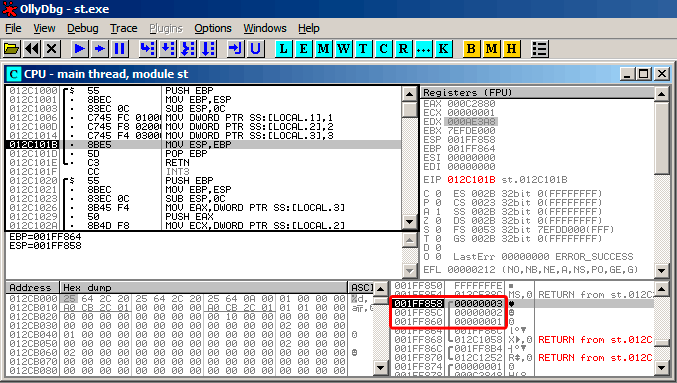
\includegraphics[scale=\FigScale]{patterns/02_stack/08_noise/olly1.png}
\caption{\olly: \TT{f1()}}
\label{fig:stack_noise_olly1}
\end{figure}

\RU{Когда}\EN{When} \TT{f1()} \RU{заполняет переменные}\EN{assigns the variables} $a$, $b$ \AndENRU $c$ 
\RU{они сохраняются по адресу}\EN{, their values are stored at the address} \TT{0x1FF860} 
\RU{\etc{}.}\EN{and so on.}

\clearpage
\RU{А когда исполняется}\EN{And when} \TT{f2()}\EN{ executes}:

\begin{figure}[H]
\centering
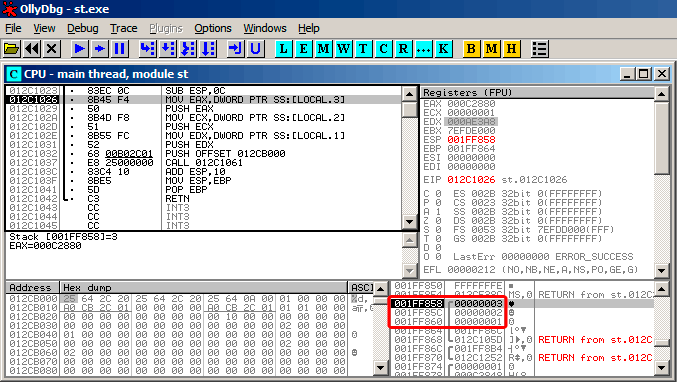
\includegraphics[scale=\FigScale]{patterns/02_stack/08_noise/olly2.png}
\caption{\olly: \TT{f2()}}
\label{fig:stack_noise_olly2}
\end{figure}

... $a$, $b$ \AndENRU $c$ \RU{в функции}\EN{of} \TT{f2()} \RU{находятся по тем же адресам!}
\EN{are located at the same addresses!}
\RU{Пока никто не перезаписал их, так что они здесь в нетронутом виде.}
\EN{No one has overwritten the values yet, so at that point they are still untouched.}

\RU{Для создания такой странной ситуации несколько функций должны исполняться друг за другом
и \ac{SP} должен быть одинаковым при входе в функции, т.е. у функций должно быть равное количество
аргументов). Тогда локальные переменные будут расположены в том же месте стека.}
\EN{So, for this weird situation to occur, several functions have to be called one after another and
\ac{SP} has to be the same at each function entry (i.e., they have the same number
of arguments). Then the local variables will be located at the same positions in the stack.}

\RU{Подводя итоги, все значения в стеке (да и памяти вообще) это значения оставшиеся от 
исполнения предыдущих функций.}
\EN{Summarizing, all values in the stack (and memory cells in general) 
have values left there from previous function executions.}
\RU{Строго говоря, они не случайны, они скорее непредсказуемы.}
\EN{They are not random in the strict sense, but rather have unpredictable values.}

\RU{А как иначе}\EN{Is there another option}?
\RU{Можно было бы очищать части стека перед исполнением каждой функции,
но это слишком много лишней (и ненужной) работы.}
\EN{It probably would be possible to clear portions of the stack before each function execution,
but that's too much extra (and unnecessary) work.}

\fi
\ifdefined\IncludeExercises
\section{\Exercises}

\subsection{\Exercise \#1}
\label{exercise_stack_1}

\RU{Если это скомпилировать в MSVC и запустить, появится три числа. Откуда они берутся? 
Откуда они берутся если скомпилировать в MSVC с оптимизациями (\Ox)?}
\EN{If we compile this piece of code in MSVC and run it, three numbers are printed.
Where do they come from?
Where do they come from if you compile it in MSVC with optimization (\Ox)?}
\RU{Почему в GCC ситуация совсем иная}\EN{Why is the situation completely different if we compile with GCC}?

\begin{lstlisting}
#include <stdio.h>

int main()
{
	printf ("%d, %d, %d\n");

	return 0;
};
\end{lstlisting}

\Answer{}: \myref{exercise_solutions_stack_1}.

\subsection{\Exercise \#2}
\label{exercise_stack_2}

\WhatThisCodeDoes\

\begin{lstlisting}[caption=\Optimizing MSVC 2010]
$SG3103	DB	'%d', 0aH, 00H

_main	PROC
	push	0
	call	DWORD PTR __imp___time64
	push	edx
	push	eax
	push	OFFSET $SG3103 ; '%d'
	call	DWORD PTR __imp__printf
	add	esp, 16
	xor	eax, eax
	ret	0
_main	ENDP
\end{lstlisting}

\begin{lstlisting}[caption=\OptimizingKeilVI (\ARMMode)]
main PROC
        PUSH     {r4,lr}
        MOV      r0,#0
        BL       time
        MOV      r1,r0
        ADR      r0,|L0.32|
        BL       __2printf
        MOV      r0,#0
        POP      {r4,pc}
        ENDP

|L0.32|
        DCB      "%d\n",0
\end{lstlisting}

\begin{lstlisting}[caption=\OptimizingKeilVI (\ThumbMode)]
main PROC
        PUSH     {r4,lr}
        MOVS     r0,#0
        BL       time
        MOVS     r1,r0
        ADR      r0,|L0.20|
        BL       __2printf
        MOVS     r0,#0
        POP      {r4,pc}
        ENDP

|L0.20|
        DCB      "%d\n",0
\end{lstlisting}

\begin{lstlisting}[caption=\Optimizing GCC 4.9 (ARM64)]
main:
	stp	x29, x30, [sp, -16]!
	mov	x0, 0
	add	x29, sp, 0
	bl	time
	mov	x1, x0
	ldp	x29, x30, [sp], 16
	adrp	x0, .LC0
	add	x0, x0, :lo12:.LC0
	b	printf
.LC0:
	.string	"%d\n"
\end{lstlisting}

\lstinputlisting[caption=\Optimizing GCC 4.4.5 (MIPS) (IDA)]{patterns/02_stack/ex_MIPS_O3_IDA.lst}

\Answer{}: \myref{exercise_solutions_stack_2}.

\fi

\chapter{\PrintfSeveralArgumentsSectionName}

\RU{Попробуем теперь немного расширить пример \IT{\HelloWorldSectionName}~(\myref{sec:helloworld}),
написав в теле функции \main:}
\EN{Now let's extend the \IT{\HelloWorldSectionName}~(\myref{sec:helloworld}) example, replacing \printf in
the \main function body with this:}

\lstinputlisting[label=hw_c]{patterns/03_printf/1.c}

% sections
\section{x86}

% subsections:
\subsection{x86: \RU{3 аргумента}\EN{3 arguments}}

\subsubsection{MSVC}

\RU{Компилируем при помощи MSVC 2010 Express, и в итоге получим:}
\EN{When we compile it with MSVC 2010 Express we get:}

\begin{lstlisting}
$SG3830	DB	'a=%d; b=%d; c=%d', 00H

...

	push	3
	push	2
	push	1
	push	OFFSET $SG3830
	call	_printf
	add	esp, 16					; 00000010H
\end{lstlisting}

\RU{Всё почти то же, за исключением того, что теперь видно, что аргументы для \printf заталкиваются в стек в обратном порядке: самый первый аргумент заталкивается последним.}
\EN{Almost the same, but now we can see the \printf arguments are pushed onto the stack in reverse order. The first argument is pushed last.}

\RU{Кстати, вспомним, что переменные типа \Tint в 32-битной системе, как известно, имеет ширину 32 бита, это 4 байта}
\EN{By the way, variables of \Tint type in 32-bit environment have 32-bit width, that is 4 bytes}.

\RU{Итак, у нас всего 4 аргумента. $4*4 = 16$~--- именно 16 байт занимают в стеке указатель на строку плюс ещё 3 числа типа \Tint.}
\EN{So, we have 4 arguments here. $4*4 = 16$~---they occupy exactly 16 bytes in the stack: a 32-bit pointer to a string and 3 numbers of type \Tint.}

\index{x86!\Instructions!ADD}
\index{x86!\Registers!ESP}
\index{cdecl}
\RU{Когда при помощи инструкции \TT{ADD ESP, X} корректируется \glslink{stack pointer}{указатель стека} \ESP 
после вызова какой-либо функции, зачастую можно сделать вывод о том, сколько аргументов 
у вызываемой функции было, разделив X на 4.}
\EN{When the \gls{stack pointer} (\ESP register) has changed back by the \TT{ADD ESP, X}
instruction after a function 
call, often, the number of function arguments could be deduced by simply dividing X by 4.}

\RU{Конечно, это относится только к cdecl-методу передачи аргументов через стек, 
и только для 32-битной среды.}
\EN{Of course, this is specific to the \IT{cdecl} calling convention, 
and only for 32-bit environment.}

\ifx\LITE\undefined
\RU{См. также в соответствующем разделе о способах передачи аргументов через стек}
\EN{See also the calling conventions section}~(\myref{sec:callingconventions}).
\fi

\RU{Иногда бывает так, что подряд идут несколько вызовов разных функций, 
но стек корректируется только один раз, после последнего вызова:}
\EN{In certain cases where several functions return right after one another, the compiler could merge multiple \TT{\q{ADD ESP, X}} instructions into one, after the last call:}

\begin{lstlisting}
push a1
push a2
call ...
...
push a1
call ...
...
push a1
push a2
push a3
call ...
add esp, 24
\end{lstlisting}

\RU{Вот пример из реальной жизни:}
\EN{Here is a real-world example:}

\lstinputlisting[caption=x86]{patterns/03_printf/x86/add_example.lst.\LANG}

\ifdefined\IncludeOlly
\clearpage
\subsubsection{MSVC \AndENRU \olly}
\index{\olly}

\RU{Попробуем этот же пример в}\EN{Now let's try to load this example in} \olly.
\RU{Это один из наиболее популярных win32-отладчиков пользовательского режима}\EN{It is one of the most 
popular user-land win32 debuggers}.
\RU{Мы можем компилировать наш пример в}\EN{We can compile our example in} MSVC 2012 
\RU{с опцией}\EN{with} \TT{/MD} \RU{что означает линковать с библиотекой}\EN{option, which means to link 
with} \TT{MSVCR*.DLL},
\RU{чтобы импортируемые функции были хорошо видны в отладчике.}
\EN{so we can see the imported functions clearly in the debugger.}

\RU{Затем загружаем исполняемый файл в}\EN{Then load the executable in} \olly.
\RU{Самая первая точка останова в}\EN{The very first breakpoint is in} \TT{ntdll.dll}, \RU{нажмите}\EN{press} 
F9 (\RU{запустить}\EN{run}).
\RU{Вторая точка останова в}\EN{The second breakpoint is in} \ac{CRT}-\RU{коде}\EN{code}.
\RU{Теперь мы должны найти функцию}\EN{Now we have to find the} \main\EN{ function}.

\RU{Найдите этот код, прокрутив окно кода до самого верха (MSVC располагает функцию \main в самом начале секции кода)}%
\EN{Find this code by scrolling the code to the very top (MSVC allocates the \main function at the very beginning of the code section)}: 

\begin{figure}[H]
\centering
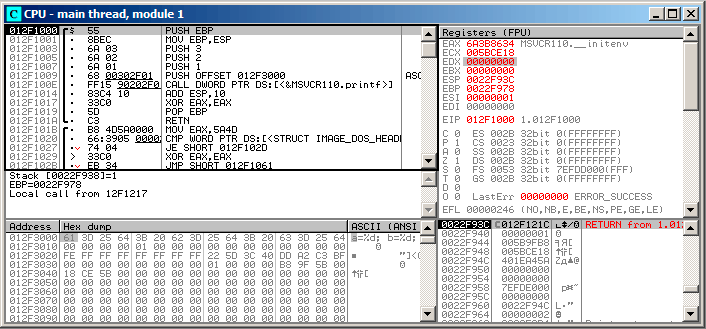
\includegraphics[scale=\FigScale]{patterns/03_printf/x86/olly3_1.png}
\caption{\olly: \RU{самое начало функции}\EN{the very start of the} \main\EN{ function}}
\label{fig:printf3_olly_1}
\end{figure}

\RU{Кликните на инструкции}\EN{Click on the} \TT{PUSH EBP}\RU{, нажмите}\EN{ instruction, press} F2 
(\RU{установка точки останова}\EN{set breakpoint}) \RU{и нажмите}\EN{and press} F9 (\RU{запустить}\EN{run}).
\RU{Нам нужно произвести все эти манипуляции, чтобы пропустить \ac{CRT}-код, потому что нам он пока
не интересен}\EN{We need to perform these actions in order to skip \ac{CRT}-code, because we aren't really
interested in it yet}.

\clearpage
\RU{Нажмите}\EN{Press} F8 (\stepover) 6 \RU{раз, т.е. пропустить
6 инструкций}\EN{times, i.e. skip 6 instructions}:

\begin{figure}[H]
\centering
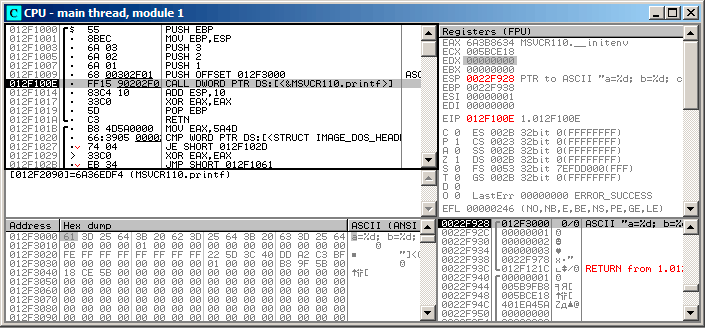
\includegraphics[scale=\FigScale]{patterns/03_printf/x86/olly3_2.png}
\caption{\olly: \RU{перед исполнением}\EN{before} \printf\EN{ execution}}
\label{fig:printf3_olly_2}
\end{figure}

\RU{Теперь}\EN{Now the} \ac{PC} \RU{указывает на инструкцию}\EN{points to the}
\TT{CALL printf}\EN{ instruction}.
\olly, \RU{как и другие отладчики, подсвечивает регистры со значениями, которые изменились.}
\EN{like other debuggers, highlights the value of the registers which were changed.}
\RU{Поэтому каждый раз когда мы нажимаем}\EN{So each time you press} F8, \EIP 
\RU{изменяется и его значение подсвечивается красным}\EN{ changes and its value is displayed in red}.
\ESP \RU{также меняется, потому что значения заталкиваются в стек}\EN{changes as well, 
because the arguments values are pushed into the stack}.\\
\\
\RU{Где находятся эти значения в стеке}\EN{Where are the values in the stack}?
\RU{Посмотрите на правое нижнее окно в отладчике}\EN{Take a look at the right bottom debugger window}:

\begin{figure}[H]
\centering
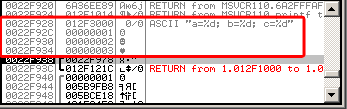
\includegraphics[scale=\NormalScale]{patterns/03_printf/x86/olly3_stack.png}
\caption{\olly: \RU{стек с сохраненными значениями}\EN{stack after the argument values have been pushed}
(\RU{красная рамка добавлена в графическом редакторе}\EN{The red rectangular border was added by me in a graphics editor})}
\end{figure}

\RU{Здесь видно 3 столбца: адрес в стеке, значение в стеке и ещё дополнительный комментарий
от \olly}\EN{We can see 3 columns there: address in the stack, 
value in the stack and some additional \olly comments}. 
\olly \RU{понимает}\EN{understands} \printf\RU{-строки}\EN{-like strings}, 
\RU{так что он показывает здесь и строку и 3 значения \IT{привязанных} к ней}\EN{so it reports the 
string here and the 3 values \IT{attached} to it}.

\RU{Можно кликнуть правой кнопкой мыши на строке формата, кликнуть на \q{Follow in dump}
и строка формата появится в окне слева внизу, где всегда виден какой-либо участок памяти}%
\EN{It is possible to right-click on the format string, click on \q{Follow in dump},
and the format string will appear in the debugger left-bottom window, which always displays some part of the memory}.
\RU{Эти значения в памяти можно редактировать}\EN{These memory values can be edited}.
\RU{Можно изменить саму строку формата, и тогда результат работы нашего примера будет другой}%
\EN{It is possible to change the format string, in which case the result of our example would be different}.
\RU{В данном случае пользы от этого немного, но для упражнения это полезно,
чтобы начать чувствовать как тут всё работает}\EN{It is not very useful in this particular case, but it could be good as an exercise so you start building a feel of how everything works here}.

\clearpage
\RU{Нажмите}\EN{Press} F8 (\stepover).

\RU{В консоли мы видим вывод}\EN{We see the following output in the console}:

\begin{figure}[H]
\centering
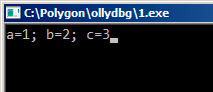
\includegraphics[scale=\NormalScale]{patterns/03_printf/x86/olly3_console.png}
\caption{\RU{Функция }\printf \RU{исполнилась}\EN{function executed}}
\end{figure}

\RU{Посмотрим как изменились регистры и состояние стека}\EN{Let's see how the registers and stack state 
have changed}: 

\begin{figure}[H]
\centering
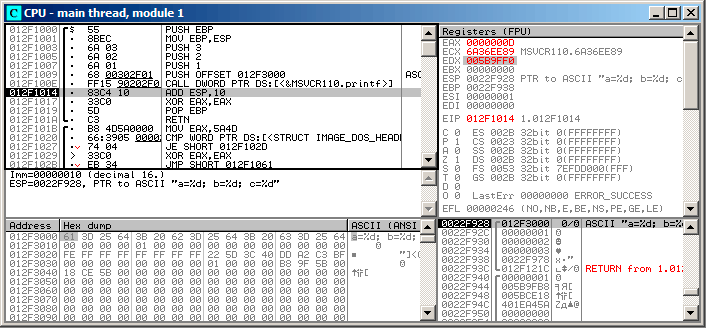
\includegraphics[scale=\FigScale]{patterns/03_printf/x86/olly3_3.png}
\caption{\olly \RU{после исполнения}\EN{after} \printf\EN{ execution}}
\label{fig:printf3_olly_3}
\end{figure}

\RU{Регистр }\EN{Register }\EAX \RU{теперь содержит}\EN{now contains} \TT{0xD} (13).
\RU{Всё верно: \printf возвращает количество выведенных символов.
Значение \EIP изменилось. Действительно, теперь здесь адрес инструкции после 
\TT{CALL printf}.}
\EN{That is correct, since \printf returns the number of characters printed. 
The value of \EIP has changed: indeed, now it contains the address of the instruction coming after 
\TT{CALL printf}.}
\RU{Значения регистров }\ECX \AndENRU \EDX \RU{также изменились}\EN{values have changed as well}.
\RU{Очевидно, внутренности функции \printf используют их для каких-то своих нужд}\EN{Apparently, the 
\printf function's hidden machinery used them for its own needs}.

\RU{Очень важно то, что значение \ESP не изменилось. И аргументы-значения в стеке также!}
\EN{A very important fact is that neither the \ESP value, nor the stack state have been changed!}
\RU{Мы ясно видим здесь и строку формата и соответствующие ей 3 значения, они всё ещё здесь.}
\EN{We clearly see that the format string and corresponding 3 values are still there.}
\RU{Действительно, по соглашению вызовов \IT{cdecl}, вызываемая функция не возвращает \ESP назад.}
\EN{This is indeed the \IT{cdecl} calling convention behaviour: \gls{callee} does not return \ESP back to its previous value.}
\RU{Это должна делать вызывающая функция}\EN{The \gls{caller} is responsible to do so}.

\clearpage
\RU{Нажмите}\EN{Press} F8 \RU{снова, чтобы исполнилась инструкция}\EN{again to execute} 
\TT{ADD ESP, 10}\EN{ instruction}:

\begin{figure}[H]
\centering
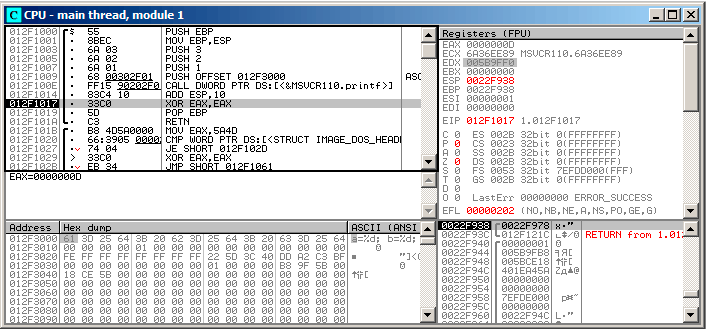
\includegraphics[scale=\FigScale]{patterns/03_printf/x86/olly3_4.png}
\caption{\olly: \RU{после исполнения инструкции}\EN{after} \TT{ADD ESP, 10}\EN{ instruction execution}}
\label{fig:printf3_olly_4}
\end{figure}

\ESP \RU{изменился, но значения всё ещё в стеке}\EN{has changed, but the values are still in the stack}!
\RU{Конечно, никому не нужно заполнять эти значения нулями или что-то в этом роде.}\EN{Yes, 
of course; no one needs to set these values to zeroes or something like that.}
\RU{Всё что выше указателя стека}\EN{Everything above the stack pointer} (\ac{SP}) 
\RU{это}\EN{is} \IT{\RU{шум}\EN{noise}} \OrENRU \IT{\garbage{}} \RU{и не имеет
особой ценности}\EN{and has no meaning at all}.
\RU{Было бы очень затратно по времени очищать ненужные элементы стека, к тому же, никому это и не 
нужно}\EN{It would be time consuming to clear the unused stack entries anyway, and no one really needs to}.

\fi

\ifdefined\IncludeGCC
\subsubsection{GCC}

\RU{Скомпилируем то же самое в Linux при помощи GCC 4.4.1 и посмотрим на результат в \IDA:}
\EN{Now let's compile the same program in Linux using GCC 4.4.1 and take a look at what we have got in \IDA:}

\begin{lstlisting}
main            proc near

var_10          = dword ptr -10h
var_C           = dword ptr -0Ch
var_8           = dword ptr -8
var_4           = dword ptr -4

                push    ebp
                mov     ebp, esp
                and     esp, 0FFFFFFF0h
                sub     esp, 10h
                mov     eax, offset aADBDCD ; "a=%d; b=%d; c=%d"
                mov     [esp+10h+var_4], 3
                mov     [esp+10h+var_8], 2
                mov     [esp+10h+var_C], 1
                mov     [esp+10h+var_10], eax
                call    _printf
                mov     eax, 0
                leave
                retn
main            endp
\end{lstlisting}

\RU{Можно сказать что этот короткий код, созданный GCC, отличается от кода MSVC только способом помещения 
значений в стек.
Здесь GCC снова работает со стеком напрямую без \PUSH/\POP.}
\EN{Its noticeable that the difference between the MSVC code and the GCC code is only in the way the arguments are stored on the stack.
Here the GCC is working directly with the stack without the use of \PUSH/\POP.}

\ifdefined\IncludeGDB
\subsubsection{GCC \AndENRU GDB}
\index{GDB}

\RU{Попробуем также этот пример и в \ac{GDB} в Linux}\EN{Let's try this example also in \ac{GDB} in Linux}.

\TT{-g} \RU{означает генерировать отладочную информацию в выходном исполняемом файле}\EN{option instructs the compiler to include debug information in the executable file}.

\begin{lstlisting}
$ gcc 1.c -g -o 1
\end{lstlisting}

\begin{lstlisting}
$ gdb 1
GNU gdb (GDB) 7.6.1-ubuntu
Copyright (C) 2013 Free Software Foundation, Inc.
License GPLv3+: GNU GPL version 3 or later <http://gnu.org/licenses/gpl.html>
This is free software: you are free to change and redistribute it.
There is NO WARRANTY, to the extent permitted by law.  Type "show copying"
and "show warranty" for details.
This GDB was configured as "i686-linux-gnu".
For bug reporting instructions, please see:
<http://www.gnu.org/software/gdb/bugs/>...
Reading symbols from /home/dennis/polygon/1...done.
\end{lstlisting}

\begin{lstlisting}[caption=\RU{установим точку останова на}\EN{let's set breakpoint on} \printf]
(gdb) b printf
Breakpoint 1 at 0x80482f0
\end{lstlisting}

\RU{Запукаем}\EN{Run}.
\RU{У нас нет исходного кода функции}\EN{We don't have the} \printf%
\RU{, поэтому \ac{GDB} не может его показать}\EN{function source code here, 
so \ac{GDB} can't show it, but may do so}.

\begin{lstlisting}
(gdb) run
Starting program: /home/dennis/polygon/1 

Breakpoint 1, __printf (format=0x80484f0 "a=%d; b=%d; c=%d") at printf.c:29
29	printf.c: No such file or directory.
\end{lstlisting}

\RU{Выдать 10 элементов стека. Левый столбец~--- это адрес в стеке.}
\EN{Print 10 stack elements. The most left column contains addresses on the stack.}

\begin{lstlisting}
(gdb) x/10w $esp
0xbffff11c:	0x0804844a	0x080484f0	0x00000001	0x00000002
0xbffff12c:	0x00000003	0x08048460	0x00000000	0x00000000
0xbffff13c:	0xb7e29905	0x00000001
\end{lstlisting}

\RU{Самый первый элемент это}\EN{The very first element is the} \ac{RA} (\TT{0x0804844a}).
\RU{Мы можем удостовериться в этом, дизассемблируя память по этому адресу}\EN{We can verify this by disassembling the memory at this address}:

\begin{lstlisting}[label=NOP_as_XCHG_example]
(gdb) x/5i 0x0804844a
   0x804844a <main+45>:	mov    $0x0,%eax
   0x804844f <main+50>:	leave  
   0x8048450 <main+51>:	ret    
   0x8048451:	xchg   %ax,%ax
   0x8048453:	xchg   %ax,%ax
\end{lstlisting}

\RU{Две инструкции \TT{XCHG} это холостые инструкции, аналогичные \ac{NOP}.}%
\EN{The two \TT{XCHG} instructions are idle instructions, analogous to \ac{NOP}s.}

\RU{Второй элемент (\TT{0x080484f0}) это адрес строки формата:}%
\EN{The second element (\TT{0x080484f0}) is the format string address:}

\begin{lstlisting}
(gdb) x/s 0x080484f0
0x80484f0:	"a=%d; b=%d; c=%d"
\end{lstlisting}

\RU{Остальные 3 элемента}\EN{Next 3 elements} (1, 2, 3) \RU{это аргументы функции}\EN{are the} 
\printf\EN{ arguments}.
\RU{Остальные элементы это может быть и мусор в стеке, но могут быть и значения
от других функций, их локальные переменные, \etc{}.}
\EN{The rest of the elements could be just \q{garbage} on the stack,
but could also be values from other functions, their local variables, \etc{}.}
\RU{Пока что мы можем игнорировать их}\EN{We can ignore them for now}.

\RU{Исполняем}\EN{Run} \q{finish}. 
\RU{Это значит исполнять все инструкции до самого конца функции}\EN{The command instructs GDB to \q{execute all instructions until the end of the function}}. 
\RU{В данном случае это означает исполнять до завершения}\EN{In this case: execute till the end of} \printf.

\begin{lstlisting}
(gdb) finish
Run till exit from #0  __printf (format=0x80484f0 "a=%d; b=%d; c=%d") at printf.c:29
main () at 1.c:6
6		return 0;
Value returned is $2 = 13
\end{lstlisting}

\ac{GDB} \RU{показывает, что вернула}\EN{shows what} \printf \RU{в}\EN{returned in} \EAX (13).
\RU{Это, так же как и в примере с \olly, количество напечатанных символов}%
\EN{This is the number of characters printed out, just like in the \olly example}.

\RU{А ещё мы видим}\EN{We also see} \q{return 0;} \RU{и что это выражение находится в файле 
\TT{1.c} в строке 6}\EN{and the information that this expression is in the \TT{1.c} file at the line 6}.
\RU{Действительно, файл \TT{1.c} лежит в текущем директории и \ac{GDB} находит там эту строку}
\EN{Indeed, the \TT{1.c} file is located in the current directory, and \ac{GDB} finds the string there}.
\RU{Как \ac{GDB} знает, какая строка Си-кода сейчас исполняется}\EN{How does \ac{GDB} know which C-code line
is being currently executed}?
\RU{Компилятор, генерируя отладочную информацию,
также сохраняет информацию о 
соответствии строк в исходном коде и адресов инструкций}\EN{This is due to the fact that the compiler,
while generating debugging information, also saves a table of relations between source code line
numbers and instruction addresses}.
GDB \RU{это всё-таки отладчик уровня исходных текстов}\EN{is a source-level debugger, after all}.

\RU{Посмотрим регистры}\EN{Let's examine the registers}.
13 \InENRU \EAX:

\begin{lstlisting}
(gdb) info registers
eax            0xd	13
ecx            0x0	0
edx            0x0	0
ebx            0xb7fc0000	-1208221696
esp            0xbffff120	0xbffff120
ebp            0xbffff138	0xbffff138
esi            0x0	0
edi            0x0	0
eip            0x804844a	0x804844a <main+45>
...
\end{lstlisting}

\RU{Попробуем дизассемблировать текущие инструкции}\EN{Let's disassemble the current instructions}.
\RU{Стрелка указывает на инструкцию, которая будет исполнена следующей}\EN{The arrow points to the 
instruction to be executed next}.

\begin{lstlisting}
(gdb) disas
Dump of assembler code for function main:
   0x0804841d <+0>:	push   %ebp
   0x0804841e <+1>:	mov    %esp,%ebp
   0x08048420 <+3>:	and    $0xfffffff0,%esp
   0x08048423 <+6>:	sub    $0x10,%esp
   0x08048426 <+9>:	movl   $0x3,0xc(%esp)
   0x0804842e <+17>:	movl   $0x2,0x8(%esp)
   0x08048436 <+25>:	movl   $0x1,0x4(%esp)
   0x0804843e <+33>:	movl   $0x80484f0,(%esp)
   0x08048445 <+40>:	call   0x80482f0 <printf@plt>
=> 0x0804844a <+45>:	mov    $0x0,%eax
   0x0804844f <+50>:	leave  
   0x08048450 <+51>:	ret    
End of assembler dump.
\end{lstlisting}

\RU{По умолчанию} \ac{GDB} \RU{показывает дизассемблированный листинг в формате}\EN{uses} AT\&T%
\EN{syntax by default}.
\RU{Но можно также переключиться в формат Intel}\EN{It is possible to switch to Intel syntax}:

\begin{lstlisting}
(gdb) set disassembly-flavor intel
(gdb) disas
Dump of assembler code for function main:
   0x0804841d <+0>:	push   ebp
   0x0804841e <+1>:	mov    ebp,esp
   0x08048420 <+3>:	and    esp,0xfffffff0
   0x08048423 <+6>:	sub    esp,0x10
   0x08048426 <+9>:	mov    DWORD PTR [esp+0xc],0x3
   0x0804842e <+17>:	mov    DWORD PTR [esp+0x8],0x2
   0x08048436 <+25>:	mov    DWORD PTR [esp+0x4],0x1
   0x0804843e <+33>:	mov    DWORD PTR [esp],0x80484f0
   0x08048445 <+40>:	call   0x80482f0 <printf@plt>
=> 0x0804844a <+45>:	mov    eax,0x0
   0x0804844f <+50>:	leave  
   0x08048450 <+51>:	ret    
End of assembler dump.
\end{lstlisting}

\RU{Исполняем следующую инструкцию}\EN{Execute next instruction}.
\ac{GDB} \RU{покажет закрывающуюся скобку, означая, что это конец блока в функции.}
\EN{shows ending bracket, meaning, it ends the block.}

\begin{lstlisting}
(gdb) step
7	};
\end{lstlisting}

\RU{Посмотрим регистры после исполнения инструкции}\EN{Let's examine the registers after the} 
\TT{MOV EAX, 0}\EN{ instruction execution}. \EN{Indeed}
\EAX \RU{здесь уже действительно ноль}\EN{is zero at that point}.

\begin{lstlisting}
(gdb) info registers
eax            0x0	0
ecx            0x0	0
edx            0x0	0
ebx            0xb7fc0000	-1208221696
esp            0xbffff120	0xbffff120
ebp            0xbffff138	0xbffff138
esi            0x0	0
edi            0x0	0
eip            0x804844f	0x804844f <main+50>
...
\end{lstlisting}
\fi
\fi

\subsection{x64: \RU{8 аргументов}\EN{8 arguments}}

\index{x86-64}
\label{example_printf8_x64}
\RU{Для того чтобы посмотреть, как остальные аргументы будут передаваться через стек, 
изменим пример ещё раз, 
увеличив количество передаваемых аргументов до 9 
(строка формата \printf и 8 переменных типа \Tint)}%
\EN{To see how other arguments are passed via the stack, let's change our example again 
by increasing the number of arguments to 9 (\printf format string + 8 \Tint variables)}:

\lstinputlisting{patterns/03_printf/2.c}

\subsubsection{MSVC}

\RU{Как уже было сказано ранее, первые 4 аргумента в Win64 передаются в регистрах}
\EN{As it was mentioned earlier, the first 4 arguments has to be passed through the} \RCX, \RDX, \Reg{8}, \Reg{9}
\RU{, а остальные~--- через стек}\EN{ registers in Win64, while all the rest---via the stack}.
\RU{Здесь мы это и видим}\EN{That is exactly what we see here}.
\RU{Впрочем, инструкция \PUSH не используется, вместо неё при помощи \MOV значения сразу записываются в стек}%
\EN{However, the \MOV instruction, instead of \PUSH, is used for preparing the stack, so the values are stored
to the stack in a straightforward manner}.

\lstinputlisting[caption=MSVC 2012 x64]{patterns/03_printf/x86/2_MSVC_x64.asm.\LANG}

\RU{Наблюдательный читатель может спросить, почему для значений типа \Tint отводится 8 байт,
ведь нужно только 4?}
\EN{The observant reader may ask why are 8 bytes allocated for \Tint values, when 4 is enough?}
\RU{Да, это нужно запомнить: для значений всех типов более коротких чем 64-бита, отводится 8 байт.}
\EN{Yes, one has to remember: 8 bytes are allocated for any data type shorter than 64 bits.}
\RU{Это сделано для удобства: так всегда легко рассчитать адрес того или иного аргумента.}
\EN{This is established for the convenience's sake: it makes it easy to calculate the address of arbitrary argument.}
\RU{К тому же, все они расположены по выровненным адресам в памяти.}
\EN{Besides, they are all located at aligned memory addresses.}
% also for local variables?
\RU{В 32-битных средах точно также: для всех типов резервируется 4 байта в стеке.}
\EN{It is the same in the 32-bit environments: 4 bytes are reserved for all data types.}

\ifdefined\IncludeGCC
\subsubsection{GCC}

\RU{В *NIX-системах для x86-64 ситуация похожая, вот только первые 6 аргументов передаются через}
\EN{The picture is similar for x86-64 *NIX OS-es, except that the first 6 arguments are passed through the} \RDI, \RSI,
\RDX, \RCX, \Reg{8}, \Reg{9}\EN{ registers}.
\RU{Остальные~--- через стек}\EN{All the rest---via the stack}.
\RU{GCC генерирует код, записывающий указатель на строку в \EDI вместо \RDI~--- 
это мы уже рассмотрели чуть раньше}\EN{GCC generates the code storing the string pointer into \EDI instead of \RDI{}---we noted that previously}: \myref{hw_EDI_instead_of_RDI}.

\RU{Почему перед вызовом \printf очищается регистр \EAX мы уже рассмотрели ранее}%
\EN{We also noted earlier that the \EAX register has been cleared before a \printf call}: \myref{SysVABI_input_EAX}.

\lstinputlisting[caption=\Optimizing GCC 4.4.6 x64]{patterns/03_printf/x86/2_GCC_x64.s.\LANG}

\ifdefined\IncludeGDB
\subsubsection{GCC + GDB}
\index{GDB}

\RU{Попробуем этот пример в}\EN{Let's try this example in} \ac{GDB}.

\begin{lstlisting}
$ gcc -g 2.c -o 2
\end{lstlisting}

\begin{lstlisting}
$ gdb 2
GNU gdb (GDB) 7.6.1-ubuntu
Copyright (C) 2013 Free Software Foundation, Inc.
License GPLv3+: GNU GPL version 3 or later <http://gnu.org/licenses/gpl.html>
This is free software: you are free to change and redistribute it.
There is NO WARRANTY, to the extent permitted by law.  Type "show copying"
and "show warranty" for details.
This GDB was configured as "x86_64-linux-gnu".
For bug reporting instructions, please see:
<http://www.gnu.org/software/gdb/bugs/>...
Reading symbols from /home/dennis/polygon/2...done.
\end{lstlisting}

\begin{lstlisting}[caption=\RU{ставим точку останова на \printf{,} запускаем}\EN{let's set the breakpoint to \printf{,} and run}]
(gdb) b printf
Breakpoint 1 at 0x400410
(gdb) run
Starting program: /home/dennis/polygon/2 

Breakpoint 1, __printf (format=0x400628 "a=%d; b=%d; c=%d; d=%d; e=%d; f=%d; g=%d; h=%d\n") at printf.c:29
29	printf.c: No such file or directory.
\end{lstlisting}

\RU{В регистрах}\EN{Registers} \RSI/\RDX/\RCX/\Reg{8}/\Reg{9} 
\RU{всё предсказуемо}\EN{have the expected values}.
\RU{А }\RIP \RU{содержит адрес самой первой инструкции функции}\EN{has the address of the very first instruction
of the} \printf\EN{ function}.

\begin{lstlisting}
(gdb) info registers
rax            0x0	0
rbx            0x0	0
rcx            0x3	3
rdx            0x2	2
rsi            0x1	1
rdi            0x400628	4195880
rbp            0x7fffffffdf60	0x7fffffffdf60
rsp            0x7fffffffdf38	0x7fffffffdf38
r8             0x4	4
r9             0x5	5
r10            0x7fffffffdce0	140737488346336
r11            0x7ffff7a65f60	140737348263776
r12            0x400440	4195392
r13            0x7fffffffe040	140737488347200
r14            0x0	0
r15            0x0	0
rip            0x7ffff7a65f60	0x7ffff7a65f60 <__printf>
...
\end{lstlisting}

\begin{lstlisting}[caption=\RU{смотрим на строку формата}\EN{let's inspect the format string}]
(gdb) x/s $rdi
0x400628:	"a=%d; b=%d; c=%d; d=%d; e=%d; f=%d; g=%d; h=%d\n"
\end{lstlisting}

\RU{Дампим стек на этот раз с командой x/g}\EN{Let's dump the stack with the x/g command this time}\EMDASH{}g 
\RU{означает}\EN{stands for} \IT{giant words}, \RU{т.е. 64-битные слова}\EN{i.e., 64-bit words}.

\begin{lstlisting}
(gdb) x/10g $rsp
0x7fffffffdf38:	0x0000000000400576	0x0000000000000006
0x7fffffffdf48:	0x0000000000000007	0x00007fff00000008
0x7fffffffdf58:	0x0000000000000000	0x0000000000000000
0x7fffffffdf68:	0x00007ffff7a33de5	0x0000000000000000
0x7fffffffdf78:	0x00007fffffffe048	0x0000000100000000
\end{lstlisting}

\RU{Самый первый элемент стека, как и в прошлый раз, это}\EN{The very first stack element, 
just like in the previous case, is the} \ac{RA}.
\RU{Через стек также передаются 3 значения}\EN{3 values are also passed through the stack}: 6, 7, 8.
\RU{Видно, что 8 передается с неочищенной старшей 32-битной частью}\EN{We also see that 8 is passed
with the high 32-bits not cleared}: \TT{0x00007fff00000008}.
\RU{Это нормально, ведь передаются числа типа \Tint, а они 32-битные}\EN{That's OK, because the values have
\Tint type, which is 32-bit}.
\RU{Так что в старшей части регистра или памяти стека остался \q{случайный мусор}}\EN{So, the high register
or stack element part may contain \q{random garbage}}.

\RU{\ac{GDB} показывает всю функцию \main, если попытаться посмотреть, куда вернется управление после исполнения \printf}%
\EN{If you take a look at where the control will return after the \printf execution,
\ac{GDB} will show the entire \main function}:

\begin{lstlisting}
(gdb) set disassembly-flavor intel
(gdb) disas 0x0000000000400576
Dump of assembler code for function main:
   0x000000000040052d <+0>:	push   rbp
   0x000000000040052e <+1>:	mov    rbp,rsp
   0x0000000000400531 <+4>:	sub    rsp,0x20
   0x0000000000400535 <+8>:	mov    DWORD PTR [rsp+0x10],0x8
   0x000000000040053d <+16>:	mov    DWORD PTR [rsp+0x8],0x7
   0x0000000000400545 <+24>:	mov    DWORD PTR [rsp],0x6
   0x000000000040054c <+31>:	mov    r9d,0x5
   0x0000000000400552 <+37>:	mov    r8d,0x4
   0x0000000000400558 <+43>:	mov    ecx,0x3
   0x000000000040055d <+48>:	mov    edx,0x2
   0x0000000000400562 <+53>:	mov    esi,0x1
   0x0000000000400567 <+58>:	mov    edi,0x400628
   0x000000000040056c <+63>:	mov    eax,0x0
   0x0000000000400571 <+68>:	call   0x400410 <printf@plt>
   0x0000000000400576 <+73>:	mov    eax,0x0
   0x000000000040057b <+78>:	leave  
   0x000000000040057c <+79>:	ret    
End of assembler dump.
\end{lstlisting}

\RU{Заканчиваем исполнение \printf, исполняем инструкцию обнуляющую \EAX, 
удостоверяемся что в регистре \EAX именно ноль}\EN{Let's finish executing \printf, execute the instruction
zeroing \EAX, and note that the \EAX register has a value of exactly zero}.
\RIP \RU{указывает сейчас на инструкцию}\EN{now points to the} \TT{LEAVE}\RU{, т.е. предпоследнюю в функции \main}
\EN{ instruction, i.e., the penultimate one in the \main function}.

\begin{lstlisting}
(gdb) finish
Run till exit from #0  __printf (format=0x400628 "a=%d; b=%d; c=%d; d=%d; e=%d; f=%d; g=%d; h=%d\n") at printf.c:29
a=1; b=2; c=3; d=4; e=5; f=6; g=7; h=8
main () at 2.c:6
6		return 0;
Value returned is $1 = 39
(gdb) next
7	};
(gdb) info registers
rax            0x0	0
rbx            0x0	0
rcx            0x26	38
rdx            0x7ffff7dd59f0	140737351866864
rsi            0x7fffffd9	2147483609
rdi            0x0	0
rbp            0x7fffffffdf60	0x7fffffffdf60
rsp            0x7fffffffdf40	0x7fffffffdf40
r8             0x7ffff7dd26a0	140737351853728
r9             0x7ffff7a60134	140737348239668
r10            0x7fffffffd5b0	140737488344496
r11            0x7ffff7a95900	140737348458752
r12            0x400440	4195392
r13            0x7fffffffe040	140737488347200
r14            0x0	0
r15            0x0	0
rip            0x40057b	0x40057b <main+78>
...
\end{lstlisting}
\fi
\fi


\ifdefined\IncludeARM
\section{ARM}

\subsection{ARM: \RU{3 аргумента}\EN{3 arguments}}

\RU{В ARM традиционно принята такая схема передачи аргументов в функцию: 
4 первых аргумента через регистры \Reg{0}-\Reg{3}; а остальные~--- через стек}
\EN{ARM's traditional scheme for passing arguments (calling convention) behaves as follows:
the first 4 arguments are passed through the \Reg{0}-\Reg{3} registers; the remaining arguments via the stack}.
\RU{Это немного похоже на то, как аргументы передаются в}\EN{This resembles the arguments passing scheme in} 
fastcall~(\myref{fastcall}) \OrENRU win64~(\myref{sec:callingconventions_win64}).

\subsubsection{32-\RU{битный}\EN{bit} ARM}

\myparagraph{\NonOptimizingKeilVI (\ARMMode)}

\begin{lstlisting}[caption=\NonOptimizingKeilVI (\ARMMode)]
.text:00000000 main
.text:00000000 10 40 2D E9   STMFD   SP!, {R4,LR}
.text:00000004 03 30 A0 E3   MOV     R3, #3
.text:00000008 02 20 A0 E3   MOV     R2, #2
.text:0000000C 01 10 A0 E3   MOV     R1, #1
.text:00000010 08 00 8F E2   ADR     R0, aADBDCD     ; "a=%d; b=%d; c=%d"
.text:00000014 06 00 00 EB   BL      __2printf
.text:00000018 00 00 A0 E3   MOV     R0, #0          ; return 0
.text:0000001C 10 80 BD E8   LDMFD   SP!, {R4,PC}
\end{lstlisting}

\RU{Итак, первые 4 аргумента передаются через регистры \Reg{0}-\Reg{3}, по порядку: 
указатель на формат-строку для \printf
в \Reg{0}, затем 1 в \Reg{1}, 2 в \Reg{2} и 3 в \Reg{3}.}
\EN{So, the first 4 arguments are passed via the \Reg{0}-\Reg{3} registers in this order:
a pointer to the \printf format string in 
\Reg{0}, then 1 in \Reg{1}, 2 in \Reg{2} and 3 in \Reg{3}.}

\RU{Инструкция на}\EN{The instruction at} \TT{0x18} \RU{записывает}\EN{writes} 0 \RU{в}\EN{to} \Reg{0}%
\EMDASH{}\RU{это выражение в Си}\EN{this is} \IT{return 0}\EN{ C-statement}.

\RU{Пока что здесь нет ничего необычного}\EN{There is nothing unusual so far}.

\OptimizingKeilVI \RU{генерирует точно такой же код}\EN{generates the same code}.

\myparagraph{\OptimizingKeilVI (\ThumbMode)}

\begin{lstlisting}[caption=\OptimizingKeilVI (\ThumbMode)]
.text:00000000 main
.text:00000000 10 B5        PUSH    {R4,LR}
.text:00000002 03 23        MOVS    R3, #3
.text:00000004 02 22        MOVS    R2, #2
.text:00000006 01 21        MOVS    R1, #1
.text:00000008 02 A0        ADR     R0, aADBDCD     ; "a=%d; b=%d; c=%d"
.text:0000000A 00 F0 0D F8  BL      __2printf
.text:0000000E 00 20        MOVS    R0, #0
.text:00000010 10 BD        POP     {R4,PC}
\end{lstlisting}

\RU{Здесь нет особых отличий от неоптимизированного варианта для режима ARM.}
\EN{There is no significant difference from the non-optimized code for ARM mode.}

\myparagraph{\OptimizingKeilVI (\ARMMode) + \RU{убираем}\EN{let's remove} return}
\label{ARM_B_to_printf}

\RU{Немного переделаем пример, убрав}\EN{Let's rework example slightly by removing} \IT{return 0}:

\begin{lstlisting}
#include <stdio.h>

void main()
{
	printf("a=%d; b=%d; c=%d", 1, 2, 3);
};
\end{lstlisting}

\RU{Результат получится необычным:}
\EN{The result is somewhat unusual:}

\begin{lstlisting}[caption=\OptimizingKeilVI (\ARMMode)]
.text:00000014 main
.text:00000014 03 30 A0 E3   MOV     R3, #3
.text:00000018 02 20 A0 E3   MOV     R2, #2
.text:0000001C 01 10 A0 E3   MOV     R1, #1
.text:00000020 1E 0E 8F E2   ADR     R0, aADBDCD     ; "a=%d; b=%d; c=%d\n"
.text:00000024 CB 18 00 EA   B       __2printf
\end{lstlisting}

\index{ARM!\Registers!Link Register}
\index{ARM!\Instructions!B}
\index{Function epilogue}
\RU{Это оптимизированная версия (\Othree) для режима ARM, и здесь мы видим последнюю инструкцию 
\TT{B} вместо привычной нам \TT{BL}}\EN{This is the optimized (\Othree) version for ARM mode and this time we see \TT{B} as the last instruction instead of the familiar \TT{BL}}.
\RU{Отличия между этой оптимизированной версией и предыдущей, скомпилированной без оптимизации, 
ещё и в том, 
что здесь нет пролога и эпилога функции (инструкций, сохраняющих состояние регистров \TT{\Reg{0}} и \ac{LR})}%
\EN{Another difference between this optimized version and the previous one (compiled without optimization)
is the lack of function prologue and epilogue (instructions preserving the \TT{\Reg{0}} and \ac{LR} registers values)}.
\index{x86!\Instructions!JMP}
\RU{Инструкция \TT{B} просто переходит на другой адрес, без манипуляций с регистром \ac{LR}, то есть
это аналог \JMP в x86}%
\EN{The \TT{B} instruction just jumps to another address, without any manipulation of the \ac{LR} register,
similar to \JMP in x86}.
\RU{Почему это работает нормально? Потому что этот код эквивалентен предыдущему.}
\EN{Why does it work? Because this code is, in fact, effectively equivalent to the previous.}
\RU{Основных причин две: 1) стек не модифицируется, как и \glslink{stack pointer}{указатель стека} \ac{SP}; 2) вызов функции \printf последний, 
после него ничего не происходит}\EN{There are two main reasons: 1) neither the stack nor \ac{SP} (the \gls{stack pointer}) is modified;
2) the call to \printf is the last instruction, so there is nothing going on afterwards}.
\RU{Функция \printf, отработав, просто возвращает управление по адресу, записанному в \ac{LR}.}
\EN{On completion, the \printf function simply returns the control to the address 
stored in \ac{LR}.}
\RU{Но в \ac{LR} находится адрес места, откуда была вызвана наша функция!
А следовательно, управление из \printf вернется сразу туда.}
\EN{Since the \ac{LR} currently stores the address of the point from where our function
was called then the control from \printf will be returned to that point.}
\RU{Значит нет нужды сохранять \ac{LR}, потому что нет нужны модифицировать \ac{LR}}%
\EN{Therefore we do not need to save \ac{LR} because we do not need to modify \ac{LR}}.
\RU{А нет нужды модифицировать \ac{LR}, потому что нет иных вызовов функций, кроме \printf, к тому же, после этого вызова не нужно ничего здесь больше делать}%
\EN{And we do not need to modify \ac{LR} because there are no other function calls except \printf. Furthermore,
after this call we do not to do anything else}!
\RU{Поэтому такая оптимизация возможна}\EN{That is the reason such optimization is possible}.

\RU{Эта оптимизация часто используется в функциях, где последнее выражение~--- это вызов другой функции.}
\EN{This optimization is often used in functions where the last statement is a call to another function.}

\RU{Ещё один похожий пример описан здесь}\EN{A similar example is presented here}:
\myref{jump_to_last_printf}.

\subsubsection{ARM64}

\myparagraph{\NonOptimizing GCC (Linaro) 4.9}

\lstinputlisting[caption=\NonOptimizing GCC (Linaro) 4.9]{patterns/03_printf/ARM/ARM3_O0.lst.\LANG}

\index{ARM!\Instructions!STP}
\RU{Итак, первая инструкция STP (Store Pair) сохраняет \ac{FP} (X29) и \ac{LR} (X30) в стеке.}
\EN{The first instruction STP (Store Pair) saves \ac{FP} (X29) and \ac{LR} (X30) in the stack.}
\RU{Вторая инструкция \TT{ADD X29, SP, 0} формирует стековый фрейм.}
\EN{The second \TT{ADD X29, SP, 0} instruction forms the stack frame.}
\RU{Это просто запись значения \ac{SP} в X29.}
\EN{It is just writing the value of \ac{SP} into X29.}

\index{ARM!\Instructions!ADRP/ADD pair}
\RU{Далее уже знакомая пара инструкций \TT{ADRP}/\ADD формирует указатель на строку.}%
\EN{Next, we see the familiar \TT{ADRP}/\ADD instruction pair, which forms a pointer to the string.}
\index{ARM64!lo12}
\RU{\IT{lo12} означает младшие 12 бит, т.е., линкер запишет младшие 12 бит адреса метки LC1 в опкод инструкции \ADD.}%
\EN{\IT{lo12} meaning low 12 bits, i.e., linker will write low 12 bits of LC1 address into the opcode of \ADD instruction.}

\RU{\TT{\%d} в формате \printf это 32-битный \Tint, так что 1, 2 и 3 заносятся в 32-битные части регистров.}
\EN{\TT{\%d} in \printf string format is a 32-bit \Tint, so the 1, 2 and 3 are loaded into 32-bit register parts.}

\Optimizing GCC (Linaro) 4.9 \RU{генерирует почти такой же код}\EN{generates the same code}.

\subsection{ARM: \RU{8 аргументов}\EN{8 arguments}}

\RU{Снова воспользуемся примером с 9-ю аргументами из предыдущей секции}\EN{Let's use again the example
with 9 arguments from the previous section}: \myref{example_printf8_x64}.

\lstinputlisting{patterns/03_printf/2.c}

\subsubsection{\OptimizingKeilVI: \ARMMode}

\begin{lstlisting}
.text:00000028             main
.text:00000028
.text:00000028             var_18 = -0x18
.text:00000028             var_14 = -0x14
.text:00000028             var_4  = -4
.text:00000028
.text:00000028 04 E0 2D E5  STR    LR, [SP,#var_4]!
.text:0000002C 14 D0 4D E2  SUB    SP, SP, #0x14
.text:00000030 08 30 A0 E3  MOV    R3, #8
.text:00000034 07 20 A0 E3  MOV    R2, #7
.text:00000038 06 10 A0 E3  MOV    R1, #6
.text:0000003C 05 00 A0 E3  MOV    R0, #5
.text:00000040 04 C0 8D E2  ADD    R12, SP, #0x18+var_14
.text:00000044 0F 00 8C E8  STMIA  R12, {R0-R3}
.text:00000048 04 00 A0 E3  MOV    R0, #4
.text:0000004C 00 00 8D E5  STR    R0, [SP,#0x18+var_18]
.text:00000050 03 30 A0 E3  MOV    R3, #3
.text:00000054 02 20 A0 E3  MOV    R2, #2
.text:00000058 01 10 A0 E3  MOV    R1, #1
.text:0000005C 6E 0F 8F E2  ADR    R0, aADBDCDDDEDFDGD ; "a=%d; b=%d; c=%d; d=%d; e=%d; f=%d; g=%"...
.text:00000060 BC 18 00 EB  BL     __2printf
.text:00000064 14 D0 8D E2  ADD    SP, SP, #0x14
.text:00000068 04 F0 9D E4  LDR    PC, [SP+4+var_4],#4
\end{lstlisting}

\RU{Этот код можно условно разделить на несколько частей}\EN{This code can be divided into several parts}:

\begin{itemize}
\index{Function prologue}
\item \RU{Пролог функции}\EN{Function prologue}:

\index{ARM!\Instructions!STR}
\RU{Самая первая инструкция}\EN{The very first} \TT{STR LR, [SP,\#var\_4]!} 
\RU{сохраняет в стеке \ac{LR}, ведь нам придется использовать этот регистр для вызова \printf}%
\EN{instruction saves \ac{LR} on the stack, because we are going to use this register for the \printf call}.
\RU{Восклицательный знак в конце означает}\EN{Exclamation mark at the end indicates} \IT{pre-index}.
\RU{Это значит, что в начале \ac{SP} должно быть
уменьшено на 4, затем по адресу в \ac{SP} должно быть записано значение \ac{LR}.}
\EN{This implies that \ac{SP} is to be decreased by 4 first, and then \ac{LR} will be saved at the address stored in \ac{SP}.}
\RU{Это аналог знакомой в x86 инструкции \PUSH}\EN{This is similar to \PUSH in x86}.
\RU{Читайте больше об этом}\EN{Read more about it at}: \myref{ARM_postindex_vs_preindex}.

\index{ARM!\Instructions!SUB}
\RU{Вторая инструкция}\EN{The second} \TT{SUB SP, SP, \#0x14}
\RU{уменьшает \glslink{stack pointer}{указатель стека} \ac{SP}, но, на самом деле, эта процедура нужна для выделения в локальном стеке места размером \TT{0x14} (20) байт.}
\EN{instruction decreases
\ac{SP} (the \gls{stack pointer}) in order to 
allocate \TT{0x14} (20) bytes on the stack.}
\RU{Действительно, нам нужно передать 5 32-битных значений через стек в \printf. Каждое значение занимает 4 байта, все вместе~--- $5*4=20$.}
\EN{Indeed, we need to pass 5 32-bit values via the stack to the \printf function, and each one occupies 4 bytes, which is exactly $5*4=20$.}
\RU{Остальные 4 32-битных значения будут переданы через регистры.}
\EN{The other 4 32-bit values are to be passed through registers.}

\item \RU{Передача 5, 6, 7 и 8 через стек}\EN{Passing 5, 6, 7 and 8 via the stack}:
\RU{они записываются в регистры \Reg{0}, \Reg{1}, \Reg{2} и \Reg{3} соответственно}%
\EN{they are stored in the \Reg{0}, \Reg{1}, \Reg{2} and \Reg{3} registers respectively}.
\RU{Затем инструкция}\EN{Then, the} \TT{ADD R12, SP, \#0x18+var\_14} 
\RU{записывает в регистр \TT{R12} адрес места в стеке, куда будут помещены эти 4 значения}%
\EN{instruction writes the stack address where these 4 variables are to be stored, into the \TT{R12} register}.
\index{IDA!var\_?}
\IT{var\_14}\RU{~--- это макрос ассемблера}\EN{ is an assembly macro}, \RU{равный}\EN{equal to} -0x14\RU{.}
\RU{Такие макросы создает \IDA, чтобы удобнее было показывать, как код обращается к стеку.}
\EN{, created by \IDA to conveniently display the code accessing the stack.}
\RU{Макросы \IT{var\_?}, создаваемые \IDA, отражают локальные переменные в стеке}\EN{The \IT{var\_?} macros generated
by \IDA reflect local variables in the stack.}
\RU{Так что в \TT{R12} будет записано \TT{SP+4}.}
\EN{So, \TT{SP+4} is to be stored into the \TT{R12} register.}
\index{ARM!\Instructions!STMIA}
\RU{Следующая инструкция}\EN{The next} \TT{STMIA R12, {R0-R3}} 
\RU{записывает содержимое регистров \Reg{0}-\Reg{3} по адресу в памяти, на который указывает \TT{R12}.}
\EN{instruction
writes registers \Reg{0}-\Reg{3} contents to the memory pointed by \TT{R12}.}
\RU{Инструкция }\TT{STMIA} \RU{означает}\EN{abbreviates} \IT{Store Multiple Increment After}. 
\IT{\q{Increment After}} 
\RU{означает, что \TT{R12} будет увеличиваться на 4 после записи каждого значения регистра.}
\EN{implies that \TT{R12} is to be increased by 4 after each register value is written.}

\item \RU{Передача 4 через стек}\EN{Passing 4 via the stack}:
\RU{4 записывается в \Reg{0}, затем инструкция}\EN{4 is stored in \Reg{0} and then
this value, with the help of the} \TT{STR R0, [SP,\#0x18+var\_18]} \RU{записывает его в стек}\EN{instruction is saved
on the stack}.
\IT{var\_18} \RU{равен}\EN{is} -0x18, \RU{смещение будет 0}\EN{so the offset is to be 0}, 
\RU{так что значение из регистра \Reg{0} (4) запишется туда, куда указывает \ac{SP}}%
\EN{thus the value from the \Reg{0} register (4) is to be written to the address written in \ac{SP}}.

\item \RU{Передача 1, 2 и 3 через регистры}\EN{Passing 1, 2 and 3 via registers}:

\RU{Значения для первых трех чисел (a, b, c) (1, 2, 3 соответственно) передаются в регистрах 
\Reg{1}, \Reg{2} и \Reg{3} перед самим вызовом \printf}%
\EN{The values of the first 3 numbers (a, b, c) (1, 2, 3 respectively) are passed through the 
\Reg{1}, \Reg{2} and \Reg{3}
registers right before the \printf call}, \RU{а остальные 5 значений передаются через стек, и вот как}\EN{and the other
5 values are passed via the stack}:

\item \RU{Вызов \printf}\EN{\printf call}.

\index{Function epilogue}
\item \RU{Эпилог функции}\EN{Function epilogue}:

\RU{Инструкция}\EN{The} \TT{ADD SP, SP, \#0x14} \RU{возвращает \ac{SP} на прежнее место, 
аннулируя таким образом всё, что было записано в стеке}%
\EN{instruction restores the \ac{SP} pointer back to its former value,
thus cleaning the stack}.
\RU{Конечно, то что было записано в стек, там пока и останется, но всё это будет многократно 
перезаписано во время исполнения последующих функций.}
\EN{Of course, what was stored on the stack will stay there, but it will all be
rewritten during the execution of subsequent functions.}

\index{ARM!\Instructions!LDR}
\RU{Инструкция}\EN{The} \TT{LDR PC, [SP+4+var\_4],\#4} \RU{загружает в \ac{PC} 
сохраненное значение \ac{LR} из стека, обеспечивая таким образом выход из функции.}
\EN{instruction loads the saved \ac{LR} value from the stack into the \ac{PC} register, 
thus causing the function to exit.}
\EN{There is no exclamation mark---indeed, \ac{PC} is loaded first from the address stored in \ac{SP} }
\RU{Здесь нет восклицательного знака~--- действительно, сначала \ac{PC} загружается из места,
куда указывает \ac{SP}}
($4+var\_4=4+(-4)=0$, \RU{так что эта инструкция аналогична}\EN{so this instruction is 
analogous to} \TT{LDR PC, [SP],\#4}), \RU{затем}\EN{and then} \ac{SP} \RU{увеличивается 
на}\EN{is increased by} 4.
\RU{Это называется}\EN{This is referred as} \IT{post-index}\footnote{\RU{Читайте больше об 
этом}\EN{Read more about it}: \myref{ARM_postindex_vs_preindex}.}.
\RU{Почему}\EN{Why does} \IDA \RU{показывает инструкцию именно так}\EN{display the instruction like that}?
\RU{Потому что она хочет показать разметку стека и тот факт, что}\EN{Because it wants to illustrate the stack layout and the fact that} \TT{var\_4} \RU{выделена в локальном стеке именно для сохраненного
значения}\EN{is allocated for saving the} \ac{LR}\EN{ value in the local stack}.
\RU{Эта инструкция в каком-то смысле аналогична}\EN{This instruction is somewhat 
similar to} \TT{POP PC} \InENRU x86\footnote{\EN{It is impossible to
set \TT{IP/EIP/RIP} value using \POP in x86, but anyway, you got the analogy right}\RU{В x86 
невозможно установить значение \TT{IP/EIP/RIP} используя \POP, но будем надеятся, вы поняли аналогию}.}.

\end{itemize}

\subsubsection{\OptimizingKeilVI: \ThumbMode}

\begin{lstlisting}
.text:0000001C             printf_main2
.text:0000001C
.text:0000001C             var_18 = -0x18
.text:0000001C             var_14 = -0x14
.text:0000001C             var_8  = -8
.text:0000001C
.text:0000001C 00 B5        PUSH    {LR}
.text:0000001E 08 23        MOVS    R3, #8
.text:00000020 85 B0        SUB     SP, SP, #0x14
.text:00000022 04 93        STR     R3, [SP,#0x18+var_8]
.text:00000024 07 22        MOVS    R2, #7
.text:00000026 06 21        MOVS    R1, #6
.text:00000028 05 20        MOVS    R0, #5
.text:0000002A 01 AB        ADD     R3, SP, #0x18+var_14
.text:0000002C 07 C3        STMIA   R3!, {R0-R2}
.text:0000002E 04 20        MOVS    R0, #4
.text:00000030 00 90        STR     R0, [SP,#0x18+var_18]
.text:00000032 03 23        MOVS    R3, #3
.text:00000034 02 22        MOVS    R2, #2
.text:00000036 01 21        MOVS    R1, #1
.text:00000038 A0 A0        ADR     R0, aADBDCDDDEDFDGD ; "a=%d; b=%d; c=%d; d=%d; e=%d; f=%d; g=%"...
.text:0000003A 06 F0 D9 F8  BL      __2printf
.text:0000003E
.text:0000003E             loc_3E   ; CODE XREF: example13_f+16
.text:0000003E 05 B0        ADD     SP, SP, #0x14
.text:00000040 00 BD        POP     {PC}
\end{lstlisting}

\RU{Это почти то же самое что и в предыдущем примере, только код для Thumb и значения помещаются в 
стек немного иначе: сначала 8 за первый раз, затем 5, 6, 7 за второй раз и 4 за третий раз}\EN{The output is almost 
like in
the previous example. However, this is Thumb code and the values are packed into stack differently: 
8 goes first, then 5, 6, 7, and 4 goes third}.

\subsubsection{\OptimizingXcodeIV: \ARMMode}

\begin{lstlisting}
__text:0000290C             _printf_main2
__text:0000290C
__text:0000290C             var_1C = -0x1C
__text:0000290C             var_C  = -0xC
__text:0000290C
__text:0000290C 80 40 2D E9   STMFD  SP!, {R7,LR}
__text:00002910 0D 70 A0 E1   MOV    R7, SP
__text:00002914 14 D0 4D E2   SUB    SP, SP, #0x14
__text:00002918 70 05 01 E3   MOV    R0, #0x1570
__text:0000291C 07 C0 A0 E3   MOV    R12, #7
__text:00002920 00 00 40 E3   MOVT   R0, #0
__text:00002924 04 20 A0 E3   MOV    R2, #4
__text:00002928 00 00 8F E0   ADD    R0, PC, R0
__text:0000292C 06 30 A0 E3   MOV    R3, #6
__text:00002930 05 10 A0 E3   MOV    R1, #5
__text:00002934 00 20 8D E5   STR    R2, [SP,#0x1C+var_1C]
__text:00002938 0A 10 8D E9   STMFA  SP, {R1,R3,R12}
__text:0000293C 08 90 A0 E3   MOV    R9, #8
__text:00002940 01 10 A0 E3   MOV    R1, #1
__text:00002944 02 20 A0 E3   MOV    R2, #2
__text:00002948 03 30 A0 E3   MOV    R3, #3
__text:0000294C 10 90 8D E5   STR    R9, [SP,#0x1C+var_C]
__text:00002950 A4 05 00 EB   BL     _printf
__text:00002954 07 D0 A0 E1   MOV    SP, R7
__text:00002958 80 80 BD E8   LDMFD  SP!, {R7,PC}
\end{lstlisting}

\index{ARM!\Instructions!STMFA}
\index{ARM!\Instructions!STMIB}
\RU{Почти то же самое, что мы уже видели, за исключением того, что}%
\EN{Almost the same as what we have already seen, with the
exception of} \TT{STMFA} (Store Multiple Full Ascending)%
\RU{~--- это синоним инструкции }\EN{ instruction, which is a synonym of}%
\TT{STMIB} (Store Multiple Increment Before)\EN{ instruction}. 
\RU{Эта инструкция увеличивает \ac{SP} и только затем записывает в память значение очередного регистра, 
но не наоборот}\EN{This
instruction increases the value in the \ac{SP} register and only then writes the next register value into the memory, rather than performing those two actions in the opposite order}.

\RU{Далее бросается в глаза то, что инструкции как будто бы расположены случайно}\EN{Another thing
that catches the eye is that the instructions are arranged seemingly random}.
\RU{Например, значение в регистре \Reg{0} подготавливается в трех местах, по адресам \TT{0x2918}, \TT{0x2920} 
и \TT{0x2928}, 
когда это можно было бы сделать в одном месте}\EN{For example, the value in the \Reg{0} register is manipulated in three
places, at addresses \TT{0x2918}, \TT{0x2920} and \TT{0x2928}, when it would be possible to do it in one point}.
\RU{Однако, у оптимизирующего компилятора могут быть свои доводы о том, как лучше составлять инструкции 
друг с другом для лучшей эффективности исполнения}%
\EN{However, the optimizing compiler may have its own reasons on how to order the instructions so to achieve higher efficiency during the execution}.
\RU{Процессор обычно пытается исполнять одновременно идущие друг за другом инструкции}%
\EN{Usually, the processor attempts to simultaneously execute instructions located side-by-side}.
\RU{К примеру, инструкции}\EN{For example, instructions like} \TT{MOVT R0, \#0} \AndENRU 
\TT{ADD R0, PC, R0} \RU{не могут быть исполнены одновременно, потому что обе инструкции модифицируют 
регистр \Reg{0}}\EN{cannot be executed simultaneously since they both modify the \Reg{0} register}. 
\RU{А вот инструкции}\EN{On the other hand,} \TT{MOVT R0, \#0} \AndENRU \TT{MOV R2, \#4} 
\RU{легко можно исполнить одновременно, 
потому что эффекты от их исполнения никак не конфликтуют друг с другом}\EN{instructions can be executed
simultaneously since the effects of their execution are not conflicting with each other}.
\RU{Вероятно, компилятор старается генерировать код именно таким образом там, где это возможно}%
\EN{Presumably, the compiler tries to generate code in such a manner (wherever it is possible)}.
 
\subsubsection{\OptimizingXcodeIV: \ThumbTwoMode}

\begin{lstlisting}
__text:00002BA0               _printf_main2
__text:00002BA0
__text:00002BA0               var_1C = -0x1C
__text:00002BA0               var_18 = -0x18
__text:00002BA0               var_C  = -0xC
__text:00002BA0
__text:00002BA0 80 B5          PUSH     {R7,LR}
__text:00002BA2 6F 46          MOV      R7, SP
__text:00002BA4 85 B0          SUB      SP, SP, #0x14
__text:00002BA6 41 F2 D8 20    MOVW     R0, #0x12D8
__text:00002BAA 4F F0 07 0C    MOV.W    R12, #7
__text:00002BAE C0 F2 00 00    MOVT.W   R0, #0
__text:00002BB2 04 22          MOVS     R2, #4
__text:00002BB4 78 44          ADD      R0, PC  ; char *
__text:00002BB6 06 23          MOVS     R3, #6
__text:00002BB8 05 21          MOVS     R1, #5
__text:00002BBA 0D F1 04 0E    ADD.W    LR, SP, #0x1C+var_18
__text:00002BBE 00 92          STR      R2, [SP,#0x1C+var_1C]
__text:00002BC0 4F F0 08 09    MOV.W    R9, #8
__text:00002BC4 8E E8 0A 10    STMIA.W  LR, {R1,R3,R12}
__text:00002BC8 01 21          MOVS     R1, #1
__text:00002BCA 02 22          MOVS     R2, #2
__text:00002BCC 03 23          MOVS     R3, #3
__text:00002BCE CD F8 10 90    STR.W    R9, [SP,#0x1C+var_C]
__text:00002BD2 01 F0 0A EA    BLX      _printf
__text:00002BD6 05 B0          ADD      SP, SP, #0x14
__text:00002BD8 80 BD          POP      {R7,PC}
\end{lstlisting}

\RU{Почти то же самое, что и в предыдущем примере,
лишь за тем исключением, что здесь используются Thumb-инструкции}%
\EN{The output is almost the same as in the previous example,
with the exception that Thumb-instructions are used instead}.
% FIXME: also STMIA is used instead of STMIB,
% which is why it uses LR, which is 4 bytes ahead of SP

\subsubsection{ARM64}

\myparagraph{\NonOptimizing GCC (Linaro) 4.9}

\lstinputlisting[caption=\NonOptimizing GCC (Linaro) 4.9]{patterns/03_printf/ARM/ARM8_O0.lst.\LANG}

\RU{Первые 8 аргументов передаются в X- или W-регистрах}\EN{The first 8 arguments are passed 
in X- or W-registers}: \cite{ARM64_PCS}.
\RU{Указатель на строку требует 64-битного регистра, так что он передается в}\EN{A string pointer 
requires a 64-bit register, so it's passed in} \RegX{0}.
\RU{Все остальные значения имеют 32-битный тип \Tint, так что они записываются в 32-битные
части регистров (W-).}
\EN{All other values have a \Tint 32-bit type, so they are stored in the 32-bit part of 
the registers (W-).}
\RU{Девятый аргумент (8) передается через стек.}
\EN{The 9th argument (8) is passed via the stack.}
\RU{Действительно, невозможно передать большое количество аргументов в регистрах, потому
что количество регистров ограничено.}
\EN{Indeed: it's not possible to pass large number of arguments through registers, 
because the number of registers is limited.}

\Optimizing GCC (Linaro) 4.9 \RU{генерирует почти такой же код}\EN{generates the same code}.


\fi
\ifdefined\IncludeMIPS
\section{MIPS}

\subsection{3 \RU{аргумента}\EN{arguments}}

\subsubsection{\Optimizing GCC 4.4.5}

\RU{Главное отличие от примера \q{\HelloWorldSectionName} в том, что здесь на самом деле
вызывается \printf вместо \puts и ещё три аргумента передаются в регистрах}%
\EN{The main difference with the \q{\HelloWorldSectionName} example is that in this case \printf is called
instead of \puts and 3 more arguments are passed through the registers} \$5\dots \$7 (\OrENRU \$A0\dots \$A2).

\RU{Вот почему эти регистры имеют префикс A-. Это значит, что они используются для передачи аргументов.}
\EN{That is why these registers are prefixed with A-, which implies they are used for function arguments passing.}

\lstinputlisting[caption=\Optimizing GCC 4.4.5 (\assemblyOutput)]{patterns/03_printf/MIPS/printf3.O3.s.\LANG}

\lstinputlisting[caption=\Optimizing GCC 4.4.5 (IDA)]{patterns/03_printf/MIPS/printf3.O3.IDA.lst.\LANG}

\EN{\IDA has coalesced pair of \INS{LUI} and \INS{ADDIU} instructions into one \INS{LA} pseudoinstruction.
That's why there are no instruction at address 0x1C: because \INS{LA} \IT{occupies} 8 bytes.}%
\RU{\IDA объединила пару инструкций \INS{LUI} и \INS{ADDIU} в одну пседовинструкцию \INS{LA}.
Вот почему здесь нет инструкции по адресу 0x1C: потому что \INS{LA} \IT{занимает} 8 байт.}

\subsubsection{\NonOptimizing GCC 4.4.5}

\NonOptimizing GCC \RU{более многословен}\EN{is more verbose}:

\lstinputlisting[caption=\NonOptimizing GCC 4.4.5 (\assemblyOutput)]{patterns/03_printf/MIPS/printf3.O0.s.\LANG}

\lstinputlisting[caption=\NonOptimizing GCC 4.4.5 (IDA)]{patterns/03_printf/MIPS/printf3.O0.IDA.lst.\LANG}

\subsection{8 \RU{аргументов}\EN{arguments}}

\RU{Снова воспользуемся примером с 9-ю аргументами из предыдущей секции}\EN{Let's use again the example
with 9 arguments from the previous section}: \myref{example_printf8_x64}.

\lstinputlisting{patterns/03_printf/2.c}

\subsubsection{\Optimizing GCC 4.4.5}

\RU{Только 4 первых аргумента передаются в регистрах \$A0 \dots \$A3, так что остальные передаются 
через стек.}
\EN{Only the first 4 arguments are passed in the \$A0 \dots \$A3 registers, the rest are passed via the stack.}
\index{MIPS!O32}
\RU{Это соглашение о вызовах O32 (самое популярное в мире MIPS).
Другие соглашения о вызовах (например N32) могут наделять регистры другими функциями.}
\EN{This is the O32 calling convention (which is the most common one in the MIPS world).
Other calling conventions (like N32) may use the registers for different purposes.}

\index{MIPS!\Instructions!SW}
\RU{SW означает \q{Store Word} (записать слово из регистра в память).}
\EN{SW abbreviates \q{Store Word} (from register to memory).}
\RU{В MIPS нет инструкции для записи значения в память, так что для этого используется пара инструкций (LI/SW).}
\EN{MIPS lacks instructions for storing a value into memory, so an instruction pair has to be used instead (LI/SW).}

\lstinputlisting[caption=\Optimizing GCC 4.4.5 (\assemblyOutput)]{patterns/03_printf/MIPS/printf8.O3.s.\LANG}

\lstinputlisting[caption=\Optimizing GCC 4.4.5 (IDA)]{patterns/03_printf/MIPS/printf8.O3.IDA.lst.\LANG}

\subsubsection{\NonOptimizing GCC 4.4.5}

\NonOptimizing GCC \RU{более многословен}\EN{is more verbose}:

\lstinputlisting[caption=\NonOptimizing GCC 4.4.5 (\assemblyOutput)]{patterns/03_printf/MIPS/printf8.O0.s.\LANG}

\lstinputlisting[caption=\NonOptimizing GCC 4.4.5 (IDA)]{patterns/03_printf/MIPS/printf8.O0.IDA.lst.\LANG}

\fi

\section{\Conclusion{}}

\RU{Вот примерный скелет вызова функции}\EN{Here is a rough skeleton of the function call}:

\lstinputlisting[caption=x86]{patterns/03_printf/skel1.lst.\LANG}

\lstinputlisting[caption=x64 (MSVC)]{patterns/03_printf/skel2.lst.\LANG}

\ifdefined\IncludeGCC
\lstinputlisting[caption=x64 (GCC)]{patterns/03_printf/skel3.lst.\LANG}
\fi

\ifdefined\IncludeARM
\lstinputlisting[caption=ARM]{patterns/03_printf/skel4.lst.\LANG}

\lstinputlisting[caption=ARM64]{patterns/03_printf/skel5.lst.\LANG}
\fi

\ifdefined\IncludeMIPS
\index{MIPS!O32}
\lstinputlisting[caption=MIPS (\RU{соглашение о вызовах O32}\EN{O32 calling convention})]{patterns/03_printf/skel_MIPS.lst.\LANG}
\fi

\section{\RU{Кстати}\EN{By the way}}

\index{fastcall}
\RU{Кстати, разница между способом передачи параметров принятая в x86, x64, fastcall, ARM и MIPS неплохо иллюстрирует тот важный момент, что процессору, в общем, всё равно, как будут 
передаваться параметры функций. Можно создать гипотетический компилятор, который будет передавать их при 
помощи указателя на структуру с параметрами, не пользуясь стеком вообще.}
\EN{By the way, this difference between the arguments passing in x86, x64, 
fastcall, ARM and MIPS is a good illustration of the fact that the CPU is oblivious to how the arguments are passed to functions. 
It is also possible to create a hypothetical compiler able to pass arguments 
via a special structure without using stack at all.}

\ifdefined\IncludeMIPS
\index{MIPS!O32}
\RU{Регистры \$A0\dots \$A3 в MIPS так названы только для удобства (это соглашение о вызовах O32).}
\EN{MIPS \$A0 \dots \$A3 registers are labelled this way only for convenience (that is in the O32 calling convention).}
\RU{Программисты могут использовать любые другие регистры (может быть, только кроме \$ZERO) для
передачи данных или любое другое соглашение о вызовах.}
\EN{Programmers may use any other register (well, maybe except \$ZERO) 
to pass data or use any other calling convention.}
\fi

\EN{The }\ac{CPU} \RU{не знает о соглашениях о вызовах вообще}\EN{is not aware of calling conventions whatsoever}.

\RU{Можно также вспомнить, что начинающие программисты на ассемблере передают параметры 
в другие функции обычно через регистры, без всякого явного порядка, или даже через глобальные переменные.
И всё это нормально работает.}
\EN{We may also recall how newcoming assembly language programmers passing arguments into
other functions:
usually via registers, without any explicit order, or even via global variables.
Of course, it works fine.}

\chapter{scanf()}
\index{\CStandardLibrary!scanf()}
\label{label_scanf}

\RU{Теперь попробуем использовать scanf().}\EN{Now let's use scanf().}

% sections
\section{\RU{Простой пример}\EN{Simple example}}

\lstinputlisting{patterns/04_scanf/1_simple/ex1.c}

\RU{Использовать \scanf в наши времена для того, чтобы спросить у пользователя что-то\EMDASH{} 
не самая хорошая идея.
Но так мы проиллюстрируем передачу указателя на переменную типа \Tint.}
\EN{It's not clever to use \scanf for user interactions nowadays. 
But we can, however, illustrate passing a pointer to a variable of type \Tint.}

\subsection{\RU{Об указателях}\EN{About pointers}}
\index{\CLanguageElements!\Pointers}

\RU{Это одна из фундаментальных вещей в информатике.}\EN{Pointers are one of the fundamental concepts in computer science.}
\RU{Часто большой массив, структуру или объект передавать в другую функцию путем копирования данных невыгодно, 
а передать адрес массива, структуры или объекта куда проще.}
\EN{Often, passing a large array, structure or object as an argument to another function is too expensive, 
while passing their address is much cheaper.}
\RU{К тому же, если вызываемая функция (\gls{callee}) должна изменить что-то в этом большом массиве или структуре,
то возвращать её полностью так же абсурдно.}
\EN{In addition if the \gls{callee} function needs to modify something in the large array or structure received as a parameter and return back the entire structure then the situation is close to absurd.}
\RU{Так что самое простое, что можно сделать, это передать в функцию-\gls{callee} адрес массива или структуры,
и пусть \gls{callee} что-то там изменит.}
\EN{So the simplest thing to do is to pass the address of the array or structure to the \gls{callee} function,
and let it change what needs to be changed.}

\RU{Указатель в}\EN{A pointer in} \CCpp\RU{\EMDASH{}это просто адрес какого-либо места в памяти.}
\EN{ is simply an address of some memory location.}

\index{x86-64}
\RU{В x86 адрес представляется в виде 32-битного числа (т.е. занимает 4 байта), а в x86-64 как 64-битное число 
(занимает 8 байт).}
\EN{In x86, the address is represented as a 32-bit number (i.e., it occupies 4 bytes), while in x86-64 it is a 64-bit number (occupying 8 bytes).}
\RU{Кстати, отсюда негодование некоторых людей, связанное с переходом на x86-64\EMDASH{}на этой архитектуре все указатели
занимают в 2 раза больше места, в том числе и в ``дорогой'' кэш-памяти.}
\EN{By the way, that is the reason behind some people's indignation related to switching to x86-64\EMDASH{}all pointers
in the x64-architecture require twice as much space, including cache memory, which is ``expensive'' place.}

\index{\CStandardLibrary!memcpy()}
\RU{При некотором упорстве можно работать только с безтиповыми указателями (\TT{void*})}\EN{
It is possible to work with untyped pointers only, given some effort}; \RU{например,}\EN{e.g.} 
\RU{стандартная функция Си}\EN{the standard C function} \TT{memcpy()},
\RU{копирующая блок из одного места памяти в другое}\EN{that copies a block from one memory location to another}, 
\RU{принимает на вход 2 указателя типа}\EN{takes 2 pointers of type } \TT{void*}\EN{ as arguments}, 
\RU{потому что нельзя
заранее предугадать, какого типа блок вы собираетесь копировать. 
Для копирования тип данных не важен, важен только размер блока.}
\EN{since it is impossible to predict the type of the data you would like to copy. 
Data types are not important, only the block size matters.}

\RU{Также указатели широко используются, когда функции нужно вернуть более одного значения}
\EN{Pointers are also widely used when a function needs to return more than one value}
(\RU{мы ещё вернемся к этому в будущем}\EN{we are going to get back to this later}
\ifx\LITE\undefined
~(\myref{label_pointers})
\fi
).
\RU{Функция }\IT{scanf()}\RU{\EMDASH{}это как раз такой случай}\EN{ is such a case}. 
\RU{Помимо того, что этой функции нужно показать, сколько значений
было прочитано успешно, ей ещё и нужно вернуть сами значения.}
\EN{Besides the fact that the function needs to indicate how many values were successfully read, 
it also needs to return all these values.}

\RU{Тип указателя в}\EN{In} \CCpp \RU{нужен для проверки типов на стадии компиляции.}
\EN{the pointer type is only needed for compile-time type checking.}
\RU{Внутри, в скомпилированном коде, никакой информации о типах указателей нет вообще.}
\EN{Internally, in the compiled code there is no information about pointer types at all.}

\subsection{x86}

\subsubsection{MSVC}

\RU{Что получаем на ассемблере, компилируя в MSVC 2010:}
\EN{Here is what we get after compiling with MSVC 2010:}

\lstinputlisting{patterns/04_scanf/1_simple/ex1_MSVC.asm.\LANG}

\RU{Переменная \TT{x} является локальной.}\EN{\TT{x} is a local variable.} 

\RU{По стандарту \CCpp она доступна только из этой же функции и нигде более. 
Так получилось, что локальные переменные располагаются в стеке. 
Может быть, можно было бы использовать и другие варианты, но в x86 это традиционно так.}
\EN{According to the \CCpp standard it must be visible only in this function and not from any other external scope. 
Traditionally, local variables are stored on the stack. 
There are probably other ways to allocate them, but in x86 that is the way it is.}

\index{x86!\Instructions!PUSH}
\RU{Следующая после пролога инструкция \TT{PUSH ECX} не ставит своей целью сохранить 
значение регистра \ECX. 
(Заметьте отсутствие соответствующей инструкции \TT{POP ECX} в конце функции).}
\EN{The goal of the instruction following the function prologue, \TT{PUSH ECX}, is not to save the \ECX state 
(notice the absence of corresponding \TT{POP ECX} at the function's end).}

\RU{Она на самом деле выделяет в стеке 4 байта для хранения \TT{x} в будущем.} 
\EN{In fact it allocates 4 bytes on the stack for storing the \TT{x} variable.} 

\label{stack_frame}
\index{\Stack!\RU{Стековый фрейм}\EN{Stack frame}}
\index{x86!\Registers!EBP}
\RU{Доступ к \TT{x} будет осуществляться при помощи объявленного макроса \TT{\_x\$} 
(он равен -4) и регистра \EBP указывающего на текущий фрейм.}
\EN{\TT{x} is to be accessed with the assistance of the \TT{\_x\$} macro 
(it equals to -4) and the \EBP register pointing to the current frame.}

\RU{Во всё время исполнения функции \EBP указывает на текущий \glslink{stack frame}{фрейм} и через \TT{EBP+смещение}
можно получить доступ как к локальным переменным функции, так и аргументам функции.} 
\EN{Over the span of the function's execution, \EBP is pointing to the current \gls{stack frame} 
making it possible to access local variables and function arguments via \TT{EBP+offset}.}

\index{x86!\Registers!ESP}
\RU{Можно было бы использовать \ESP, но он во время исполнения функции часто меняется, а это не удобно. 
Так что можно сказать, что \EBP это \IT{замороженное состояние} \ESP на момент начала исполнения функции.}
\EN{It is also possible to use \ESP for the same purpose, although that is not very convenient since it changes frequently.
The value of the \EBP could be perceived as a \IT{frozen state} of the value in \ESP at the start of the function's execution.}

% FIXME1 это уже было в 02_stack?
\RU{Разметка типичного стекового \glslink{stack frame}{фрейма} в 32-битной среде}%
\EN{Here is a typical \gls{stack frame} layout in 32-bit environment}:

\begin{center}
\begin{tabular}{ | l | l | }
\hline
\dots & \dots \\
\hline
EBP-8 & \RU{локальная переменная}\EN{local variable} \#2, \MarkedInIDAAs{} \TT{var\_8} \\
\hline
EBP-4 & \RU{локальная переменная}\EN{local variable} \#1, \MarkedInIDAAs{} \TT{var\_4} \\
\hline
EBP & \RU{сохраненное значение}\EN{saved value of} \EBP \\
\hline
EBP+4 & \RU{адрес возврата}\EN{return address} \\
\hline
EBP+8 & \argument \#1, \MarkedInIDAAs{} \TT{arg\_0} \\
\hline
EBP+0xC & \argument \#2, \MarkedInIDAAs{} \TT{arg\_4} \\
\hline
EBP+0x10 & \argument \#3, \MarkedInIDAAs{} \TT{arg\_8} \\
\hline
\dots & \dots \\
\hline
\end{tabular}
\end{center}

\RU{У функции \scanf в нашем примере два аргумента.}\EN{The \scanf function in our example has two arguments.}

\RU{Первый~--- указатель на строку, содержащую \TT{\%d} и второй~--- адрес переменной \TT{x}.} 
\EN{The first one is a pointer to the string containing \TT{\%d} and the second is the address of the \TT{x} variable.} 

\index{x86!\Instructions!LEA}
\RU{Вначале адрес \TT{x} помещается в регистр \EAX при помощи инструкции \TT{lea eax, DWORD PTR \_x\$[ebp]}.}
\EN{First, the \TT{x} variable's address is loaded into the \EAX register by the \TT{lea eax, DWORD PTR \_x\$[ebp]} instruction}

\ifx\LITE\undefined
\RU{Инструкция \LEA означает \IT{load effective address}, и часто используется для формирования адреса чего-либо}
\EN{\LEA stands for \IT{load effective address}, and is often used for forming an address}
~(\myref{sec:LEA}).
\fi

\RU{Можно сказать, что в данном случае \LEA просто помещает в \EAX результат суммы значения в регистре 
\EBP и макроса \TT{\_x\$}.}
\EN{We could say that in this case \LEA simply stores the sum of the \EBP register value and the \TT{\_x\$} macro in the \EAX register.}

\RU{Это тоже что и}\EN{This is the same as} \TT{lea eax, [ebp-4]}.

\RU{Итак, от значения \EBP отнимается 4 и помещается в \EAX.
Далее значение \EAX заталкивается в стек и вызывается \scanf.}
\EN{So, 4 is being subtracted from the \EBP register value and the result is loaded in the \EAX register.
Next the \EAX register value is pushed into the stack and \scanf is being called.}

\RU{После этого вызывается \printf. Первый аргумент вызова строка:} 
\EN{\printf is being called after that with its first argument --- a pointer to the string:} \TT{You entered \%d...\textbackslash{}n}.

\RU{Второй аргумент: \TT{mov ecx, [ebp-4]}. Эта инструкция помещает в \ECX не адрес переменной \TT{x}, 
а её значение.}
\EN{The second argument is prepared with: \TT{mov ecx, [ebp-4]}.
The instruction stores the \TT{x} variable value and not its address, in the \ECX register.}

\RU{Далее значение \ECX заталкивается в стек и вызывается \printf.}
\EN{Next the value in the \ECX is stored on the stack and the last \printf is being called.}

\ifdefined\IncludeOlly
\input{patterns/04_scanf/1_simple/olly.tex}
\fi

\ifdefined\IncludeGCC
\subsubsection{GCC}

\RU{Попробуем тоже самое скомпилировать в Linux при помощи GCC 4.4.1:}
\EN{Let's try to compile this code in GCC 4.4.1 under Linux:}

\lstinputlisting{patterns/04_scanf/1_simple/ex1_GCC.asm}

\index{puts() \RU{вместо}\EN{instead of} printf()}
\RU{GCC заменил первый вызов \printf на \puts. Почему это было сделано, 
уже было описано ранее~(\myref{puts}).}
\EN{GCC replaced the \printf call with call to \puts. The reason for this was explained in ~(\myref{puts}).}

% TODO: rewrite
%\RU{Почему \scanf переименовали в \TT{\_\_\_isoc99\_scanf}, я честно говоря, пока не знаю.}
%\EN{Why \scanf is renamed to \TT{\_\_\_isoc99\_scanf}, I do not know yet.}
% 
% Apparently it has to do with the ISO c99 standard compliance. By default GCC allows specifying a standard to adhere to.
% For example if you compile with -std=c89 the outputted assmebly file will contain scanf and not __isoc99__scanf. I guess current GCC version adhares to c99 by default.
% According to my understanding the two implementations differ in the set of suported modifyers (See printf man page)


\RU{Далее всё как и прежде~--- параметры заталкиваются через стек при помощи \MOV.}
\EN{As in the MSVC example---the arguments are placed on the stack using the \MOV instruction.}
\fi

\subsubsection{\RU{Кстати}\EN{By the way}}

\RU{Кстати, этот простой пример иллюстрирует то обстоятельство, что компилятор преобразует
список выражений в \CCpp-блоке просто в последовательный набор инструкций.}
\EN{By the way, this simple example is a demonstration of the fact that compiler translates
list of expressions in \CCpp-block into sequential list of instructions.}
\RU{Между выражениями в \CCpp ничего нет, и в итоговом машинном коде между ними тоже ничего нет, 
управление переходит от одной инструкции к следующей за ней.}
\EN{There are nothing between expressions in \CCpp, and so in resulting machine code, 
there are nothing between, control flow slips from one expression to the next one.}

\subsection{x64}

\index{x86-64}
\RU{Всё то же самое, только используются регистры вместо стека для передачи аргументов функций}%
\EN{The picture here is similar with the difference that the registers, rather than the stack, are used for arguments passing}.

\subsubsection{MSVC}

\lstinputlisting[caption=MSVC 2012 x64]{patterns/04_scanf/1_simple/ex1_MSVC_x64.asm.\LANG}

\ifdefined\IncludeGCC
\subsubsection{GCC}

\lstinputlisting[caption=\Optimizing GCC 4.4.6 x64]{patterns/04_scanf/1_simple/ex1_GCC_x64.s.\LANG}
\fi


\ifdefined\IncludeARM
\subsection{ARM}

\subsubsection{\OptimizingKeilVI (\ThumbMode)}

\begin{lstlisting}
.text:00000042             scanf_main
.text:00000042
.text:00000042             var_8           = -8
.text:00000042
.text:00000042 08 B5                       PUSH    {R3,LR}
.text:00000044 A9 A0                       ADR     R0, aEnterX     ; "Enter X:\n"
.text:00000046 06 F0 D3 F8                 BL      __2printf
.text:0000004A 69 46                       MOV     R1, SP
.text:0000004C AA A0                       ADR     R0, aD          ; "%d"
.text:0000004E 06 F0 CD F8                 BL      __0scanf
.text:00000052 00 99                       LDR     R1, [SP,#8+var_8]
.text:00000054 A9 A0                       ADR     R0, aYouEnteredD___ ; "You entered %d...\n"
.text:00000056 06 F0 CB F8                 BL      __2printf
.text:0000005A 00 20                       MOVS    R0, #0
.text:0000005C 08 BD                       POP     {R3,PC}
\end{lstlisting}

\index{\CLanguageElements!\Pointers}
\RU{Чтобы \scanf мог вернуть значение, ему нужно передать указатель на переменную типа \Tint.}
\EN{In order for \scanf to be able to read item it needs a parameter---pointer to an \Tint.}
\Tint\RU{~--- 32-битное значение, для его хранения нужно только 4 байта, и оно помещается в 
32-битный регистр.}
\EN{is 32-bit, so we need 4 bytes to store it somewhere in memory, and it fits exactly 
in a 32-bit register.}
\index{IDA!var\_?}
\RU{Место для локальной переменной \TT{x} выделяется в стеке, \IDA наименовала её \IT{var\_8}. 
Впрочем, место для неё выделять не обязательно, т.к. \glslink{stack pointer}{указатель стека} \ac{SP} уже указывает на место, 
свободное для использования.}\EN{A place for the local variable \TT{x} is allocated in the stack and \IDA
has named it \IT{var\_8}. It is not necessary, however, to allocate a such since \ac{SP} (\gls{stack pointer}) is already pointing to that space and it can be used directly.}
\RU{Так что значение указателя \ac{SP} копируется в регистр \Reg{1}, и вместе с format-строкой, 
передается в \scanf.}
\EN{So, \ac{SP}'s value is copied to the \Reg{1} register and, together with the format-string, passed
to \scanf.}
\index{ARM!\Instructions!LDR}
\RU{Позже, при помощи инструкции \TT{LDR}, это значение перемещается из стека в регистр \Reg{1}, 
чтобы быть переданным в \printf.}\EN{Later, with the help of the \TT{LDR} instruction, this value is moved
from the stack to the \Reg{1} register in order to be passed to \printf.}

\subsubsection{ARM64}

\lstinputlisting[caption=\NonOptimizing GCC 4.9.1 ARM64,numbers=left]{patterns/04_scanf/1_simple/ARM64_GCC491_O0.s.\LANG}

\RU{Под стековый фрейм выделяется 32 байта, что больше чем нужно. Вероятно, это связано с выравниваем по границе памяти?}%
\EN{There is 32 bytes are allocated for stack frame, which is bigger than it needed. Perhaps, some memory aligning issue?}
\RU{Самая интересная часть~--- это поиск места под переменную $x$ в стековом фрейме (строка 22).}
\EN{The most interesting part is finding space for the $x$ variable in the stack frame (line 22).}
\RU{Почему 28? Почему-то, компилятор решил расположить эту переменную в конце стекового фрейма, а не в начале.}%
\EN{Why 28? Somehow, compiler decided to place this variable at the end of stack frame instead of beginning.}
\RU{Адрес потом передается в \scanf, которая просто сохраняет значение, введенное пользователем, в памяти
по этому адресу.}
\EN{The address is passed to \scanf, which just stores the user input value in the memory at that address.}
\RU{Это 32-битное значение типа \Tint}\EN{This is 32-bit value of type \Tint}.
\RU{Значение загружается в строке 27 и затем передается в \printf.}
\EN{The value is fetched at line 27 and then passed to \printf.}


\fi
\ifdefined\IncludeMIPS
\subsection{MIPS}

\RU{Для переменной $x$ выделено место в стеке, и к нему будут производиться обращения как $\$sp+24$.}
\EN{A place in the local stack is allocated for the $x$ variable, and it is to be referred as $\$sp+24$.}
\index{MIPS!\Instructions!LW}
\RU{Её адрес передается в \scanf, а значение прочитанное от пользователя загружается используя 
инструкцию LW (\q{Load Word}~--- загрузить слово) и затем оно передается в \printf.}
\EN{Its address is passed to \scanf, and the user input values is loaded using the LW (\q{Load Word}) instruction
and then passed to \printf.}

\lstinputlisting[caption=\Optimizing GCC 4.4.5 (\assemblyOutput)]{patterns/04_scanf/1_simple/MIPS/ex1.O3.s.\LANG}

\RU{IDA показывает разметку стека следующим образом:}
\EN{IDA displays the stack layout as follows:}

\lstinputlisting[caption=\Optimizing GCC 4.4.5 (IDA)]{patterns/04_scanf/1_simple/MIPS/ex1.O3.IDA.lst.\LANG}

% TODO non-optimized version?

\fi

\section{\RU{Глобальные переменные}\EN{Global variables}}
\index{\RU{Глобальные переменные}\EN{Global variables}}
\label{scanf_global_variable}

\RU{А что если переменная \TT{x} из предыдущего примера будет глобальной переменной, а не локальной? 
Тогда к ней смогут обращаться из любого другого места, а не только из тела функции. 
Глобальные переменные считаются \glslink{anti-pattern}{анти-паттерном},
но ради примера мы можем себе это позволить.}
\EN{What if the \TT{x} variable from the previous example was not local but a global one? 
Then it would have been accessible from any point, not only from the function body. 
Global variables are considered \gls{anti-pattern}, but for the sake of the experiment, we could do this.}

\lstinputlisting{patterns/04_scanf/2_global/ex2.c.\LANG}

\subsection{MSVC: x86}

\lstinputlisting{patterns/04_scanf/2_global/ex2_MSVC.asm}

\RU{В целом ничего особенного. Теперь \TT{x} объявлена в сегменте \TT{\_DATA}. 
Память для неё в стеке более не выделяется.
Все обращения к ней происходит не через стек, а уже напрямую. 
Неинициализированные глобальные переменные не занимают места в исполняемом файле
(и действительно, зачем в исполняемом файле
нужно выделять место под изначально нулевые переменные?), но тогда, когда к этому месту в памяти
кто-то обратится, \ac{OS} подставит туда блок, состоящий из нулей\footnote{Так работает \ac{VM}}.}
\EN{In this case the \TT{x} variable is defined in the \TT{\_DATA} segment and no memory is allocated in the local stack. It is accessed directly, not through the stack. 
Uninitialized global variables take no space in the executable file
(indeed, why one needs to allocate space for variables initially set to zero?), 
but when someone accesses their address, 
the \ac{OS} will allocate a block of zeroes there\footnote{That is how a \ac{VM} behaves}.}

\RU{Попробуем изменить объявление этой переменной:}
\EN{Now let's explicitly assign a value to the variable:}

\lstinputlisting{patterns/04_scanf/2_global/default_value.c.\LANG}

\RU{Выйдет в итоге:}\EN{We got:}

\begin{lstlisting}
_DATA	SEGMENT
_x	DD	0aH

...
\end{lstlisting}

\RU{Здесь уже по месту этой переменной записано \TT{0xA} с типом DD (dword = 32 бита).}
\EN{Here we see a value \TT{0xA} of DWORD type (DD stands for DWORD = 32 bit) for this variable.}

\RU{Если вы откроете скомпилированный .exe-файл в \IDA, то увидите, что \IT{x} 
находится в начале сегмента \TT{\_DATA}, после этой переменной будут текстовые строки.}
\EN{If you open the compiled .exe in \IDA, you can see the \IT{x} variable placed at the beginning of 
the \TT{\_DATA} segment, and after it you can see text strings.}

\RU{А вот если вы откроете в \IDA .exe скомпилированный в прошлом примере, 
где значение \IT{x} не определено, то вы увидите:}
\EN{If you open the compiled .exe from the previous example in \IDA, where the value of \IT{x} was not
set, you would see something like this:}

\begin{lstlisting}
.data:0040FA80 _x              dd ?                    ; DATA XREF: _main+10
.data:0040FA80                                         ; _main+22
.data:0040FA84 dword_40FA84    dd ?                    ; DATA XREF: _memset+1E
.data:0040FA84                                         ; unknown_libname_1+28
.data:0040FA88 dword_40FA88    dd ?                    ; DATA XREF: ___sbh_find_block+5
.data:0040FA88                                         ; ___sbh_free_block+2BC
.data:0040FA8C ; LPVOID lpMem
.data:0040FA8C lpMem           dd ?                    ; DATA XREF: ___sbh_find_block+B
.data:0040FA8C                                         ; ___sbh_free_block+2CA
.data:0040FA90 dword_40FA90    dd ?                    ; DATA XREF: _V6_HeapAlloc+13
.data:0040FA90                                         ; __calloc_impl+72
.data:0040FA94 dword_40FA94    dd ?                    ; DATA XREF: ___sbh_free_block+2FE
\end{lstlisting}

\RU{\TT{\_x} обозначен как \TT{?}, наряду с другими переменными не требующими инициализации. 
Это означает, что при загрузке .exe в память, место под всё это выделено будет и будет заполнено
нулевыми байтами \cite[6.7.8p10]{C99TC3}. 
Но в самом .exe ничего этого нет. Неинициализированные переменные не занимают места в исполняемых файлах. 
Это удобно для больших массивов, например.}
\EN{\TT{\_x} is marked with \TT{?} with the rest of the variables that do not need to be initialized. 
This implies that after loading the .exe to the memory, a space for all these variables is to be 
allocated and filled with zeroes \cite[6.7.8p10]{C99TC3}. 
But in the .exe file these uninitialized variables do not occupy anything.
This is convenient for large arrays, for example.}

\ifdefined\IncludeOlly
\input{patterns/04_scanf/2_global/olly.tex}
\fi

\ifdefined\IncludeGCC
\subsection{GCC: x86}

\index{ELF}
\RU{В Linux всё почти также. За исключением того, что если значение \TT{x} не определено, 
то эта переменная будет находится в сегменте \TT{\_bss}.
В \ac{ELF} этот сегмент имеет такие атрибуты:}
\EN{The picture in Linux is near the same, with the difference that the uninitialized variables are located in the \TT{\_bss} segment. 
In \ac{ELF} file this segment has the following attributes:}

\begin{lstlisting}
; Segment type: Uninitialized
; Segment permissions: Read/Write
\end{lstlisting}

\RU{Ну а если сделать статическое присвоение этой переменной какого-либо
значения, например, 10, то она будет находится 
в сегменте \TT{\_data},
это сегмент с такими атрибутами:}
\EN{If you, however, initialise the variable with some value e.g. 10, 
it is to be placed in the \TT{\_data} segment, which has the following attributes:}

\begin{lstlisting}
; Segment type: Pure data
; Segment permissions: Read/Write
\end{lstlisting}
\fi

\subsection{MSVC: x64}

\lstinputlisting[caption=MSVC 2012 x64]{patterns/04_scanf/2_global/ex2_MSVC_x64.asm.\LANG}

\RU{Почти такой же код как и в}\EN{The code is almost the same as in} x86.
\RU{Обратите внимание что для \TT{scanf()} адрес переменной $x$ передается
при помощи инструкции \LEA, а во второй \printf передается само значение переменной при помощи \MOV}
\EN{Please note that the address of the $x$ variable is passed to \TT{scanf()} using a \LEA instruction,
while the variable's value is passed to the second \printf using a \MOV instruction}.
\TT{DWORD PTR}\RU{\EMDASH{}это часть языка ассемблера (не имеющая отношения к машинным кодам) 
показывающая, что тип переменной в памяти именно 32-битный, 
и инструкция \MOV должна быть здесь закодирована соответственно}\EN{ is a part of the assembly language (no relation to the machine code), indicating that the variable data size is 32-bit and the \MOV instruction
has to be encoded accordingly}.

\ifdefined\IncludeARM
\subsection{ARM: \OptimizingKeilVI (\ThumbMode)}

\begin{lstlisting}
.text:00000000 ; Segment type: Pure code
.text:00000000                 AREA .text, CODE
...
.text:00000000 main
.text:00000000                 PUSH    {R4,LR}
.text:00000002                 ADR     R0, aEnterX     ; "Enter X:\n"
.text:00000004                 BL      __2printf
.text:00000008                 LDR     R1, =x
.text:0000000A                 ADR     R0, aD          ; "%d"
.text:0000000C                 BL      __0scanf
.text:00000010                 LDR     R0, =x
.text:00000012                 LDR     R1, [R0]
.text:00000014                 ADR     R0, aYouEnteredD___ ; "You entered %d...\n"
.text:00000016                 BL      __2printf
.text:0000001A                 MOVS    R0, #0
.text:0000001C                 POP     {R4,PC}
...
.text:00000020 aEnterX         DCB "Enter X:",0xA,0    ; DATA XREF: main+2
.text:0000002A                 DCB    0
.text:0000002B                 DCB    0
.text:0000002C off_2C          DCD x                   ; DATA XREF: main+8
.text:0000002C                                         ; main+10
.text:00000030 aD              DCB "%d",0              ; DATA XREF: main+A
.text:00000033                 DCB    0
.text:00000034 aYouEnteredD___ DCB "You entered %d...",0xA,0 ; DATA XREF: main+14
.text:00000047                 DCB 0
.text:00000047 ; .text         ends
.text:00000047
...
.data:00000048 ; Segment type: Pure data
.data:00000048                 AREA .data, DATA
.data:00000048                 ; ORG 0x48
.data:00000048                 EXPORT x
.data:00000048 x               DCD 0xA                 ; DATA XREF: main+8
.data:00000048                                         ; main+10
.data:00000048 ; .data         ends
\end{lstlisting}

\RU{Итак, переменная \TT{x} теперь глобальная, и она расположена, почему-то, в другом сегменте, а именно сегменте данных}
\EN{So, the \TT{x} variable is now global and for this reason located in another segment, namely the data segment} (\IT{.data}).
\RU{Можно спросить, почему текстовые строки расположены в сегменте кода (\IT{.text}), а \TT{x} нельзя было разместить тут же?}
\EN{One could ask, why are the text strings located in the code segment (\IT{.text}) and \TT{x} is located right here?}
\RU{Потому что эта переменная, и как следует из определения, она может меняться. И может быть, меняться часто.}
\EN{Because it is a variable and by definition its value could change. Moreover it could possibly change often.}
\RU{Ну а текстовые строки имеют тип констант, они не будут меняться, поэтому они располагаются в сегменте \IT{.text}.}
\EN{While text strings has constant type, they will not be changed, so they are located in the \IT{.text} segment.}
\index{\RAM}
\index{\ROM}
\RU{Сегмент кода иногда может быть расположен в ПЗУ микроконтроллера (не забывайте, 
мы сейчас имеем дело с embedded-микроэлектроникой, где дефицит памяти~--- обычное дело),
а изменяемые переменные~--- в ОЗУ.}
\EN{The code segment might sometimes be located in a \ac{ROM} chip (remember, we now deal
with embedded microelectronics, and memory scarcity is common here), and changeable 
variables~---in \ac{RAM}.}
\RU{Хранить в ОЗУ неизменяемые данные, когда в наличии есть ПЗУ, не экономно.}
\EN{It is not very economical to store constant variables in RAM when you have ROM.}
\RU{К тому же, сегмент данных в ОЗУ с константами нужно инициализировать перед работой,
ведь, после включения ОЗУ, очевидно, она содержит в себе случайную информацию.}
\EN{Furthermore, constant variables in RAM must be initialized, because after powering on, the RAM, obviously, contains random information.}

\index{\RU{Компоновщик}\EN{Linker}}
\RU{Далее мы видим в сегменте кода хранится указатель на переменную \TT{x} (\TT{off\_2C}) и 
все операции с переменной происходят через этот указатель.}
\EN{Moving forward, we see a pointer to the \TT{x} (\TT{off\_2C}) variable in the code segment, and that all
operations with the variable occur via this pointer.}
\RU{Это связано с тем, что переменная \TT{x} может быть расположена где-то довольно далеко от 
данного участка кода, так что её адрес нужно сохранить в непосредственной близости к этому коду.}
\EN{That is because the \TT{x} variable could be located somewhere far from this particular code fragment, so its address
must be saved somewhere in close proximity to the code.}
\index{ARM!\Instructions!LDR}
\RU{Инструкция \TT{LDR} в Thumb-режиме может адресовать только переменные в пределах вплоть 
до 1020 байт от своего местоположения.}
\EN{The \TT{LDR} instruction in Thumb mode can only address variables in a range of 1020 bytes from its location, }
\RU{Эта же инструкция в ARM-режиме~--- переменные в пределах $\pm{}4095$ байт.}
\EN{and in in ARM-mode~---variables in range of $\pm{}4095$ bytes.}
\RU{Таким образом,
адрес глобальной переменной \TT{x} нужно расположить в непосредственной близости, ведь нет никакой гарантии, 
что компоновщик\footnote{linker в англоязычной литературе} сможет разместить саму переменную где-то рядом, 
она может быть даже в другом чипе памяти!}
\EN{And so the address of the \TT{x} variable
must be located somewhere in close proximity, because there is no guarantee that the linker would be able to accommodate the variable somewhere nearby the code, it may well be even in an external memory chip!}

\index{\CLanguageElements!const}
\index{\ROM}
\RU{Ещё одна вещь: если переменную объявить как \IT{const}, то компилятор Keil разместит её в 
сегменте \TT{.constdata}.}
\EN{One more thing: if a variable is declared as \IT{const}, the Keil compiler allocates it in 
the \TT{.constdata} segment.}
\RU{Должно быть, впоследствии компоновщик и этот сегмент сможет разместить в ПЗУ вместе
с сегментом кода.}
\EN{Perhaps, thereafter, the linker could place this segment in ROM too, along with the code segment.}

\subsection{ARM64}

\lstinputlisting[caption=\NonOptimizing GCC 4.9.1 ARM64,numbers=left]{patterns/04_scanf/2_global/ARM64_GCC491_O0.s.\LANG}

\index{ARM!\Instructions!ADRP/ADD pair}
\RU{Теперь $x$ это глобальная переменная, и её адрес вычисляется при помощи пары инструкций ADRP/ADD 
(строки 21 и 25).}
\EN{In this case the $x$ variable is declared as global and its address is calculated using 
the ADRP/ADD instruction pair (lines 21 and 25).}

\fi
\ifdefined\IncludeMIPS
\subsection{MIPS}

\subsubsection{\EN{Uninitialized global variable}\RU{Неинициализированная глобальная переменная}}

\RU{Так что теперь переменная $x$ глобальная.}
\EN{So now the $x$ variable is global.}
\RU{Сделаем исполняемый файл вместо объектного и загрузим его в \IDA.}
\EN{Let's compile to executable file rather than object file and load it into \IDA.}
\RU{IDA показывает присутствие переменной $x$ в ELF-секции .sbss (помните о \q{Global Pointer}? \myref{MIPS_GP}),
так как переменная не инициализируется в самом начале.}
\EN{IDA displays the $x$ variable in the .sbss ELF section (remember the \q{Global Pointer}? \myref{MIPS_GP}),
since the variable is not initialized at the start.}

\lstinputlisting[caption=\Optimizing GCC 4.4.5 (IDA)]{patterns/04_scanf/2_global/MIPS/O3_IDA.lst.\LANG}

\RU{IDA уменьшает количество информации, так что сделаем также листинг используя objdump и добавим туда свои комментарии:}%
\EN{IDA reduces the amount of information, so we'll also do a listing using objdump and comment it:}

\lstinputlisting[caption=\Optimizing GCC 4.4.5 (objdump),numbers=left]{patterns/04_scanf/2_global/MIPS/O3_objdump.txt.\LANG}

\RU{Теперь мы видим, как адрес переменной $x$ берется из буфера 64KiB, используя GP и прибавление
к нему отрицательного смещения (строка 18).}
\EN{Now we see the $x$ variable address is read from a 64KiB data buffer using GP and adding
negative offset to it (line 18).}
\RU{И даже более того: адреса трех внешних функций, используемых в нашем примере (\puts, \scanf, \printf)
также берутся из буфера 64KiB используя GP (строки 9, 16 и 26).}
\EN{More than that, the addresses of the three external functions  which are used in our example (\puts, \scanf, \printf), are also read from the 64KiB global data buffer using GP (lines 9, 16 and 26).}
\RU{GP указывает на середину буфера, так что такие смещения могут нам подсказать, что адреса всех трех функций,
а также адрес переменной $x$ расположены где-то в самом начале буфера.}
\EN{GP points to the middle of the buffer, and such offset suggests that all three function's addresses,
and also the address of the $x$ variable, are all stored somewhere at the beginning of that buffer.}
\RU{Действительно, ведь наш пример крохотный}\EN{That make sense, because our example is tiny}.

\index{MIPS!\Pseudoinstructions!MOVE}
\index{MIPS!\Pseudoinstructions!NOP}
\RU{Ещё нужно отметить что функция заканчивается двумя \ac{NOP}-ами (\TT{MOVE \$AT,\$AT}~--- 
это холостая инструкция), чтобы выровнять начало следующей функции по 16-байтной границе.}
\EN{Another thing worth mentioning is that the function ends with two \ac{NOP}s (\TT{MOVE \$AT,\$AT} --- 
an idle instruction), in order to align next function's start on 16-byte boundary.}

\subsubsection{\RU{Инициализированная глобальная переменная}\EN{Initialized global variable}}

\RU{Немного изменим наш пример и сделаем, чтобы у $x$ было значение по умолчанию:}
\EN{Let's alter our example by giving the $x$ variable a default value:}

\lstinputlisting{patterns/04_scanf/2_global/default_value.c.\LANG}

\RU{Теперь IDA показывает что переменная $x$ располагается в секции .data:}
\EN{Now IDA shows that the $x$ variable is residing in the .data section:}

\lstinputlisting[caption=\Optimizing GCC 4.4.5 (IDA)]{patterns/04_scanf/2_global/MIPS/O3_IDA_init.lst.\LANG}

\RU{Почему не .sdata? Может быть, нужно было указать какую-то опцию в GCC?}
\EN{Why not .sdata? Perhaps that this depends on some GCC option?}
\RU{Тем не менее, $x$ теперь в .data, а это уже общая память и мы можем посмотреть как происходит
работа с переменными там.}
\EN{Nevertheless, now $x$ is in .data, which is a general memory area, and we can take a look
how to work with variables there.}

\index{MIPS!\Instructions!LUI}
\index{MIPS!\Instructions!ADDIU}
\RU{Адрес переменной должен быть сформирован парой инструкций.}
\EN{The variable's address must be formed using a pair of instructions.}
\RU{В нашем случае это LUI (\q{Load Upper Immediate}~--- загрузить старшие 16 бит) и 
ADDIU (\q{Add Immediate Unsigned Word}~--- прибавить значение).}
\EN{In our case those are LUI (\q{Load Upper Immediate}) and ADDIU (\q{Add Immediate Unsigned Word}).}

\RU{Вот так же листинг сгенерированный objdump-ом для лучшего рассмотрения:}
\EN{Here is also the objdump listing for close inspection:}

\lstinputlisting[caption=\Optimizing GCC 4.4.5 (objdump)]{patterns/04_scanf/2_global/MIPS/O3_objdump_init.txt.\LANG}

\index{MIPS!\Instructions!LUI}
\index{MIPS!\Instructions!ADDIU}
\index{MIPS!\Instructions!LW}
\RU{Адрес формируется используя LUI и ADDIU, но старшая часть адреса
всё ещё в регистре \$S0, и можно закодировать смещение в инструкции LW (\q{Load Word}), так что одной
LW достаточно для загрузки значения из переменной и передачи его в \printf.}
\EN{We see that the address is formed using LUI and ADDIU, but the high part of address is still in
the \$S0 register, and it is possible to encode the offset in a LW (\q{Load Word}) instruction, so one single LW is enough 
to load a value from the variable and pass it to \printf.}

\RU{Регистры хранящие временные данные имеют префикс T-, но здесь есть также регистры с префиксом S-,
содержимое которых должно быть сохранено в других функциях (т.е. \q{saved}).}
\EN{Registers holding temporary data are prefixed with T-, but here we also see some prefixed with S-, 
the contents of which is need to be preserved before use in other functions (i.e., \q{saved}).}
% FIXME:
% This needs to be clarified a bit, e.g. "the registers need to be preserved if a function is called and it wants to use them
\RU{Вот почему \$S0 был установлен по адресу 0x4006cc и затем был использован по адресу 0x4006e8
после вызова \scanf.}
\EN{That is why the value of \$S0 was set at address 0x4006cc and was used again
at address 0x4006e8, after the \scanf call. }
\RU{Функция \scanf не изменяет это значение.}\EN{The \scanf function does not change its value.}

% TODO non-optimized example?

\fi

\section{\RU{Проверка результата scanf()}\EN{scanf() result checking}}

\RU {Как уже было упомянуто, использовать \scanf в наше время слегка старомодно. 
Но если уж жизнь заставила этим заниматься, нужно хотя бы проверять, сработал ли \scanf 
правильно или пользователь ввел вместо числа что-то другое, что \scanf не смог трактовать как число.}%
\EN{As was noted before, it is slightly old-fashioned to use \scanf today. 
But if we have to, we need to at least check if \scanf finishes correctly without an error.}

\lstinputlisting{patterns/04_scanf/3_checking_retval/ex3.c}

\RU{По стандарту,}\EN{By standard, the} 
\scanf\footnote{scanf, wscanf: \href{http://go.yurichev.com/17255}{MSDN}} 
\RU{возвращает количество успешно полученных значений.}
\EN{function returns the number of fields it has successfully read.}

\RU{В нашем случае, если всё успешно и пользователь ввел таки некое число, \scanf вернет 1. 
А если нет, то 0 (или \ac{EOF}).} 
\EN{In our case, if everything goes fine and the user enters a number 
\scanf returns 1, or in case of error (or \ac{EOF}) --- 0.}

\RU{Добавим код, проверяющий результат \scanf и в случае ошибки он сообщает пользователю что-то другое.}%
\EN{Let's add some C code to check the \scanf return value and print error message in case of an error.}

\RU{Это работает предсказуемо}\EN{This works as expected}:

\begin{lstlisting}
C:\...>ex3.exe
Enter X:
123
You entered 123...

C:\...>ex3.exe
Enter X:
ouch
What you entered? Huh?
\end{lstlisting}

% subsections
\subsection{MSVC: x86}

\RU{Вот что выходит на ассемблере}\EN{Here is what we get in the assembly output} (MSVC 2010):

\lstinputlisting{patterns/04_scanf/3_checking_retval/ex3_MSVC_x86.asm}

\index{x86!\Registers!EAX}
\RU{Для того чтобы вызывающая функция имела доступ к результату вызываемой функции, 
вызываемая функция (в нашем случае \scanf) оставляет это значение в регистре \EAX.}
\EN{The \gls{caller} function (\main) needs the \gls{callee} function (\scanf) result, 
so the \gls{callee} returns it in the \EAX register.}

\index{x86!\Instructions!CMP}
\RU{Мы проверяем его инструкцией \TT{CMP EAX, 1} (\IT{CoMPare}), то есть 
сравниваем значение в \EAX с 1.}
\EN{We check it with the help of the instruction \TT{CMP EAX, 1} (\IT{CoMPare}).
In other words, we compare the value in the \EAX register with 1.} 

\index{x86!\Instructions!JNE}
\RU{Следующий за инструкцией \CMP: условный переход \JNE. 
Это означает \IT{Jump if Not Equal}, то есть условный переход \IT{если не равно}.}
\EN{A \JNE conditional jump follows the \CMP instruction. \JNE stands for \IT{Jump if Not Equal}.}

\RU{Итак, если \EAX не равен 1, то \JNE заставит \ac{CPU} перейти 
по адресу указанном в операнде \JNE, у нас это \TT{\$LN2@main}.}
\EN{So, if the value in the \EAX register is not equal to 1, 
the \ac{CPU} will pass the execution to the 
address mentioned in the \JNE operand, in our case \TT{\$LN2@main}.}
\RU{Передав управление по этому адресу, \ac{CPU} начнет исполнять вызов \printf с 
аргументом \TT{What you entered? Huh?}.}
\EN{Passing the control to this address results in the \ac{CPU} executing \printf 
with the argument \TT{What you entered? Huh?}.}
\RU{Но если всё нормально, перехода не случится и исполнится другой \printf с двумя аргументами: 
\TT{'You entered \%d...'} и значением переменной \TT{x}.}
\EN{But if everything is fine, the conditional jump is not be be taken, and another \printf call 
is to be executed, with two arguments: \TT{'You entered \%d...'} and the value of \TT{x}. }

\index{x86!\Instructions!XOR}
\index{\CLanguageElements!return}
\RU{Для того чтобы после этого вызова не исполнился сразу второй вызов \printf, 
после него есть инструкция \JMP, безусловный переход, который отправит процессор на место 
после второго \printf и перед инструкцией \TT{XOR EAX, EAX}, которая реализует \TT{return 0}.}
\EN{Since in this case the second \printf has not to be executed, there is a \JMP preceding it (unconditional jump). 
It passes the control to the point after the second \printf and just before the \TT{XOR EAX, EAX} instruction, which implements \TT{return 0}.}

\index{x86!\Registers!\Flags}
\RU{Итак, можно сказать что в подавляющих случаях сравнение какой-либо переменной с чем-то другим 
происходит при помощи пары инструкций \CMP и \Jcc, где \IT{cc} это \IT{condition code}.}
\EN{So, it could be said that comparing a value with another is \IT{usually} implemented
by \CMP/\Jcc instruction pair, where \IT{cc} is \IT{condition code}.}
\RU{\CMP сравнивает два значения и выставляет 
флаги процессора\footnote{См. также о флагах x86-процессора: \href{http://go.yurichev.com/17120}{wikipedia}.}.}
\EN{\CMP compares two values and sets 
processor flags\footnote{x86 flags, see also: \href{http://go.yurichev.com/17120}{wikipedia}.}.}
\RU{\Jcc проверяет нужные ему флаги и выполняет переход по указанному адресу (или не выполняет).}
\EN{\Jcc checks those flags and decides to either pass the control to the specified address or not.}

\index{x86!\Instructions!CMP}
\index{x86!\Instructions!SUB}
\label{CMPandSUB}
\RU{Но на самом деле, как это не парадоксально поначалу звучит, \CMP это почти то же самое что и 
инструкция \SUB, которая отнимает числа одно от другого.}
\EN{This could sound paradoxical, but the \CMP instruction is in fact \SUB (subtract).}
\RU{Все арифметические инструкции также выставляют флаги в соответствии с результатом, не только \CMP.}
\EN{All arithmetic instructions set processor flags, not just \CMP.}
\RU{Если мы сравним 1 и 1, от единицы отнимется единица, получится 0, и выставится флаг 
\ZF (\IT{zero flag}), означающий, что последний полученный результат был 0.}
\EN{If we compare 1 and 1, $1-1$ is 0 so the \ZF flag would be set (meaning that the last result was 0).}
\RU{Ни при каких других значениях \EAX, флаг \ZF не может быть выставлен, кроме тех, когда операнды равны друг другу.}
\EN{In no other circumstances \ZF can be set, except when the operands are equal.}
\index{x86!\Instructions!JNE}
\index{x86!\Registers!ZF}
\RU{Инструкция \JNE проверяет только флаг \ZF, и совершает переход только если флаг не поднят. 
Фактически, \JNE это синоним инструкции \JNZ (\IT{Jump if Not Zero}).}
\EN{\JNE checks only the \ZF flag and jumps only if it is not set. 
\JNE is in fact a synonym for \JNZ (\IT{Jump if Not Zero}).}
\RU{Ассемблер транслирует обе инструкции в один и тот же опкод.}
\EN{Assembler translates both \JNE and \JNZ instructions into the same opcode.}
\RU{Таким образом, можно \CMP заменить на \SUB и всё будет работать также, но разница в том, что \SUB 
всё-таки испортит значение в первом операнде. \CMP это \IT{SUB без сохранения результата, но изменяющая флаги}.}
\EN{So, the \CMP instruction can be replaced with a \SUB instruction 
and almost everything will be fine,
with the difference that \SUB alters the value of the first operand.
\CMP is \IT{SUB without saving the result, but affecting flags}.}

\ifx\LITE\undefined
\subsection{MSVC: x86: IDA}

\index{IDA}
\RU{Наверное, уже пора делать первые попытки анализа кода в \IDA}%
\EN{It is time to run \IDA and try to do something in it}.
\RU{Кстати, начинающим полезно компилировать в MSVC с ключом \TT{/MD}, что означает что все эти стандартные
функции не будут скомпонованы с исполняемым файлом, а будут импортироваться из файла \TT{MSVCR*.DLL}.}
\EN{By the way, for beginners it is good idea to use \TT{/MD} option in MSVC, which means that all these
standard functions are not be linked with the executable file, 
but are to be imported from the \TT{MSVCR*.DLL} file instead.}
\RU{Так будет легче увидеть, где какая стандартная функция используется.}
\EN{Thus it will be easier to see which standard function are used and where.}

\RU{Анализируя код в \IDA, очень полезно делать пометки для себя (и других).}
\EN{While analysing code in \IDA, it is very helpful to leave notes for oneself (and others)}.
\RU{Например, разбирая этот пример, мы сразу видим, что \TT{JNZ} срабатывает в случае ошибки.}
\EN{In instance, analysing this example, 
we see that \TT{JNZ} is to be triggered in case of an error.}
\RU{Можно навести курсор на эту метку, нажать \q{n} и переименовать метку в \q{error}.}
\EN{So it is possible to move the cursor to the label, press \q{n} and rename it to \q{error}.}
\RU{Ещё одну метку}\EN{Create another label}\EMDASH{}\RU{в}\EN{into} \q{exit}.
\RU{Вот как у меня получилось в итоге}\EN{Here is my result}:

\lstinputlisting{patterns/04_scanf/3_checking_retval/ex3.lst}

\RU{Так понимать код становится чуть легче}\EN{Now it is slightly easier to understand the code}.
\RU{Впрочем, меру нужно знать во всем и комментировать каждую инструкцию не стоит.}
\EN{However, it is not a good idea to comment on every instruction.}

% FIXME draw button?
\RU{В \IDA также можно скрывать части функций: нужно выделить скрываемую часть, нажать \q{--} на цифровой клавиатуре и ввести текст}
\EN{You could also hide(collapse) parts of a function in \IDA.
To do that mark the block, then press \q{--} on the numerical pad and enter the text to be displayed instead}.

\RU{Скроем две части и придумаем им названия}\EN{Let's hide two blocks and give them names}:

\lstinputlisting{patterns/04_scanf/3_checking_retval/ex3_2.lst}

% FIXME draw button?
\RU{Раскрывать скрытые части функций можно при помощи \q{+} на цифровой клавиатуре}
\EN{To expand previously collapsed parts of the code, use \q{+} on the numerical pad}.

\clearpage
\RU{Нажав \q{пробел}, мы увидим, как \IDA может представить функцию в виде графа}\EN{By pressing \q{space},
we can see how \IDA represents a function as a graph}:

\begin{figure}[H]
\centering
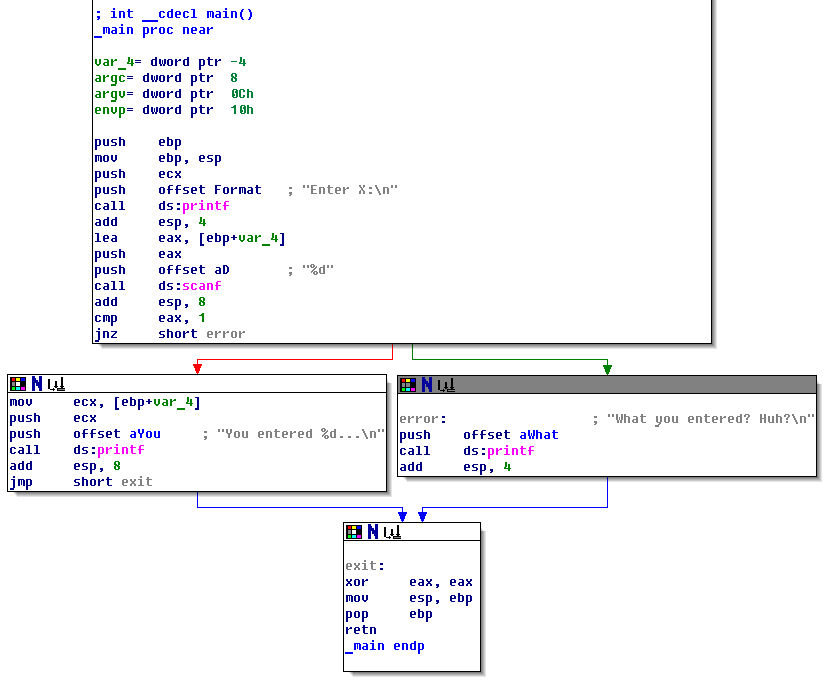
\includegraphics[scale=\FigScale]{patterns/04_scanf/3_checking_retval/IDA.png}
\caption{\RU{Отображение функции в IDA в виде графа}\EN{Graph mode in IDA}}
\label{fig:ex3_IDA_1}
\end{figure}

\RU{После каждого условного перехода видны две стрелки: зеленая и красная}\EN{There are two arrows
after each conditional jump: green and red}.
\RU{Зеленая ведет к тому блоку, который исполнится если переход сработает, 
а красная~--- если не сработает.}
\EN{The green arrow points to the block which executes if the jump is triggered, 
and red if otherwise.}

\clearpage
\RU{В этом режиме также можно сворачивать узлы и давать им названия}
\EN{It is possible to fold nodes in this mode and give them names as well} (\q{group nodes}).
\RU{Сделаем это для трех блоков}\EN{Let's do it for 3 blocks}:

\begin{figure}[H]
\centering
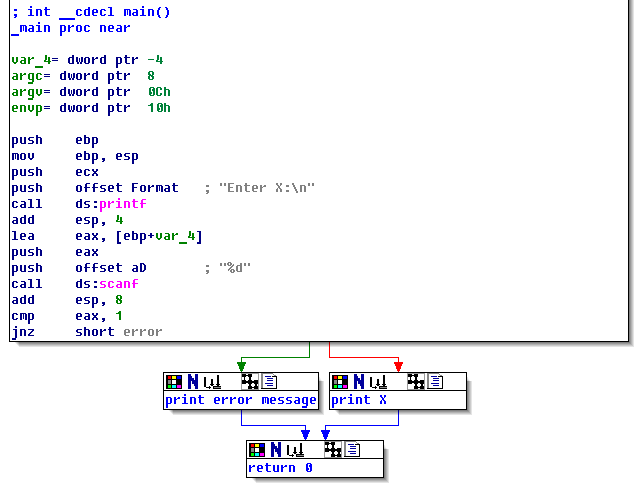
\includegraphics[scale=\FigScale]{patterns/04_scanf/3_checking_retval/IDA2.png}
\caption{\RU{Отображение в IDA в виде графа с тремя свернутыми блоками}\EN{Graph mode in IDA with 3 nodes folded}}
\label{fig:ex3_IDA_2}
\end{figure}

\RU{Всё это очень полезно делать}\EN{That is very useful}.
\RU{Вообще, очень важная часть работы реверсера (да и любого исследователя) состоит в том, чтобы уменьшать количество имеющейся информации.}
\EN{It could be said that a very important part of the reverse engineers' job (and any other researcher as well) is to reduce the amount of information they deal with.}
\fi

\ifdefined\IncludeOlly
\input{patterns/04_scanf/3_checking_retval/olly.tex}
\fi

\clearpage
\subsection{MSVC: x86 + Hiew}
\index{Hiew}

\RU{Это ещё может быть и простым примером исправления исполняемого файла}\EN{This can also be used as 
a simple example of executable file patching}.
\RU{Мы можем попробовать исправить его таким образом, что программа всегда будет выводить числа,
вне зависимости от ввода}\EN{We may try to patch the executable so the program would always 
print the input, no matter what we enter}.

\RU{Исполняемый файл скомпилирован с импортированием функций из}\EN{Assuming that the 
executable is compiled against external} \TT{MSVCR*.DLL} (\RU{т.е. с опцией}\EN{i.e., with} 
\TT{/MD}\EN{ option})\footnote{\RU{то, что ещё называют}\EN{that's what also called} \q{dynamic linking}}, 
\RU{поэтому мы можем отыскать функцию}\EN{we see the} \main \RU{в самом начале секции}\EN{function at the 
beginning of the} \TT{.text}\EN{ section}.
\RU{Откроем исполняемый файл в Hiew, найдем самое начало секции}\EN{Let's open the executable in Hiew and 
find the beginning of the} \TT{.text}\EN{ section} (Enter, F8, F6, Enter, Enter).

\RU{Мы увидим следующее}\EN{We can see this}:

\begin{figure}[H]
\centering
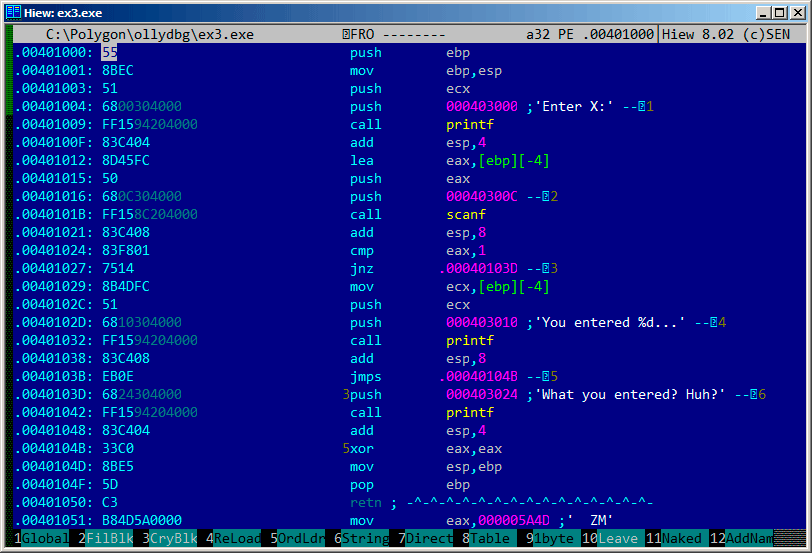
\includegraphics[scale=\FigScale]{patterns/04_scanf/3_checking_retval/hiew_1.png}
\caption{Hiew: \RU{функция }\main\EN{ function}}
\label{fig:scanf_ex3_hiew_1}
\end{figure}

Hiew \RU{находит}\EN{finds} \ac{ASCIIZ}\RU{-строки и показывает их, также как и имена импортируемых 
функций}\EN{ strings and displays them, as it does with the imported functions' names}.

\clearpage
\RU{Переведите курсор на адрес}\EN{Move the cursor to address} \TT{.00401027} 
(\RU{с инструкцией}\EN{where the} \TT{JNZ}\RU{, которую мы хотим заблокировать}\EN{ instruction, we 
have to bypass, is located}), \RU{нажмите}\EN{press} F3,
\RU{затем наберите}\EN{and then type} \q{9090}(\RU{ что означает два}\EN{, meaning two} \ac{NOP}\RU{-а}\EN{s}): 

\begin{figure}[H]
\centering
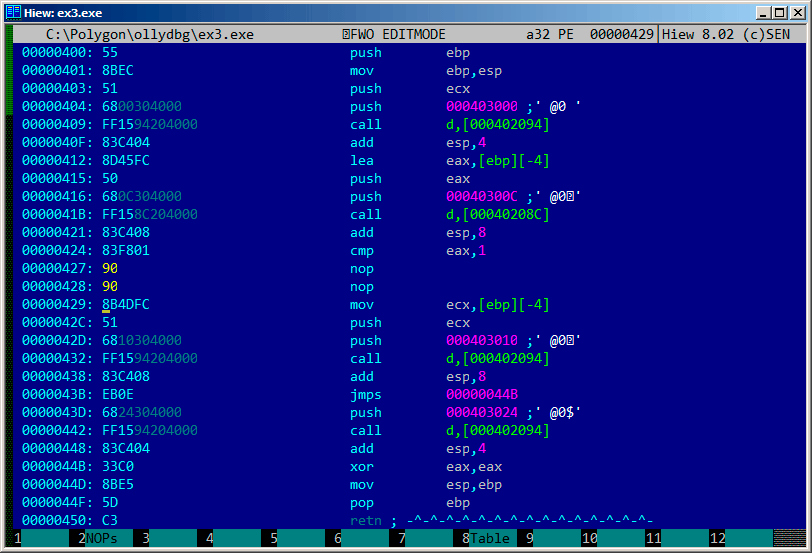
\includegraphics[scale=\FigScale]{patterns/04_scanf/3_checking_retval/hiew_2.png}
\caption{Hiew: \RU{замена}\EN{replacing} \TT{JNZ} \RU{на два}\EN{with two} \ac{NOP}\RU{-а}\EN{s}}
\label{fig:scanf_ex3_hiew_2}
\end{figure}

\RU{Затем}\EN{Then press} F9 (update). \RU{Теперь исполняемый файл записан на диск. Он будет вести себя
так, как нам надо.}\EN{Now the executable is saved to the disk. It will behave as we wanted.}

\RU{Два}\EN{Two} \ac{NOP}\RU{-а}\EN{s} \RU{возможно, не так эстетично, как могло бы быть}\EN{are probably 
not the most \ae{}sthetic approach}.
\RU{Другой способ изменить инструкцию это записать 0 во второй байт опкода (смещение перехода),
так что}\EN{Another way to patch this instruction is to write just 0 to the second opcode byte (\gls{jump offset}), 
so that} \TT{JNZ} \RU{всегда будет переходить на следующую инструкцию}\EN{will always jump to 
the next instruction}.

\RU{Можно изменить и наоборот: первый байт заменить на \TT{EB}, второй байт (смещение перехода) не трогать.}
\EN{We could also do the opposite: replace first byte with \TT{EB} while not touching the second byte (\gls{jump offset}).}
\RU{Получится всегда срабатывающий безусловный переход}\EN{We would get an unconditional jump that is always triggered}.
\RU{Теперь сообщение об ошибке будет выдаваться всегда, даже если мы ввели число.}
\EN{In this case the error message would be printed every time, no matter the input.}

\subsection{MSVC: x64}

\index{x86-64}
\RU{Так как здесь мы работаем с переменными типа \Tint, а они в x86-64 остались 32-битными, то мы здесь видим,
как продолжают использоваться регистры с префиксом \TT{E-}.}\EN{Since we work here with \Tint{}-typed variables,
which are still 32-bit in x86-64, we see how the 32-bit part of the registers (prefixed with \TT{E-}) 
are used here as well.}
\RU{Но для работы с указателями, конечно, используются 64-битные части регистров с префиксом \TT{R-}.}
\EN{While working with pointers, however, 64-bit register parts are used, prefixed with \TT{R-}.}

\lstinputlisting[caption=MSVC 2012 x64]{patterns/04_scanf/3_checking_retval/ex3_MSVC_x64.asm.\LANG}


\ifdefined\IncludeARM
\subsection{ARM}

\subsubsection{ARM: \OptimizingKeilVI (\ThumbMode)}

\lstinputlisting[caption=\OptimizingKeilVI (\ThumbMode)]{patterns/04_scanf/3_checking_retval/ex3_ARM_Keil_thumb_O3.asm}

\index{ARM!\Instructions!CMP}
\index{ARM!\Instructions!BEQ}
\RU{Здесь для нас есть новые инструкции: \CMP и \ac{BEQ}.}
\EN{The new instructions here are \CMP and \ac{BEQ}.}

\CMP \RU{аналогична той что в x86: она отнимает один аргумент от второго и сохраняет флаги.}
\EN{is analogous to the x86 instruction with the same name, it subtracts one of the arguments from the other and updates the conditional flags if needed.}
% TODO: в мануале ARM $op1 + NOT(op2) + 1$ вместо вычитания

\index{ARM!\Registers!Z}
\index{x86!\Instructions!JZ}
\ac{BEQ} \RU{совершает переход по другому адресу, 
если операнды при сравнении были равны, 
либо если результат последнего вычисления был 0, либо если флаг Z равен 1.}
\EN{jumps to another address if the operands were equal to each other, or,
if the result of the last computation was 0, or if the Z flag is 1.}
\RU{То же что и \JZ в}\EN{It behaves as \JZ in} x86.

\RU{Всё остальное просто: исполнение разветвляется на две ветки, затем они сходятся там, 
где в \Reg{0} записывается 0 как возвращаемое из функции значение и происходит выход из функции.}
\EN{Everything else is simple: the execution flow forks in two branches, then the branches
converge at the point
where 0 is written into the \Reg{0} as a function return value, and then the function ends.}

\subsubsection{ARM64}

\lstinputlisting[caption=\NonOptimizing GCC 4.9.1 ARM64,numbers=left]{patterns/04_scanf/3_checking_retval/ARM64_GCC491_O0.s.\LANG}

\index{ARM!\Instructions!CMP}
\index{ARM!\Instructions!Bcc}
\EN{Code flow in this case forks with the use of CMP/BNE (Branch if Not Equal) instructions pair.}
\RU{Исполнение здесь разветвляется, используя пару инструкций CMP/BNE (Branch if Not Equal: переход если не равно).}

\fi
\ifdefined\IncludeMIPS
\subsection{MIPS}

\lstinputlisting[caption=\Optimizing GCC 4.4.5 (IDA)]{patterns/04_scanf/3_checking_retval/MIPS_O3_IDA.lst}

\index{MIPS!\Instructions!BEQ}
\RU{\scanf возвращает результат своей работы в регистре \$V0 и он проверяется по адресу 0x004006E4
сравнивая значения в \$V0 и \$V1 (1 записан в \$V1 ранее, на 0x004006DC).}
\EN{\scanf returns the result of its work in register \$V0. It is checked at address 0x004006E4
by comparing the values in \$V0 with \$V1 (1 was stored in \$V1 earlier, at 0x004006DC).}
BEQ \EN{stands for}\RU{означает} \q{Branch Equal}\RU{ (переход если равно)}.
\RU{Если значения равны (т.е. в случае успеха), произойдет переход по адресу 0x0040070C.}
\EN{If the two values are equal (i.e., success), the execution jumps to address 0x0040070C.}

\fi

\ifdefined\IncludeExercises
\subsection{\Exercise}

\index{x86!\Instructions!Jcc}
\index{ARM!\Instructions!Bcc}
\EN{As we can see, the JNE/JNZ instruction can be easily replaced by the JE/JZ and vice versa 
(or BNE by BEQ and vice versa).}
\RU{Как мы можем увидеть, инструкцию JNE/JNZ можно вполне заменить на JE/JZ или наоборот 
(или BNE на BEQ и наоборот).}
\EN{But then the basic blocks must also be swapped.}\RU{Но при этом ещё нужно переставить базовые блоки местами.}
\EN{Try to do this in some of the examples.}\RU{Попробуйте сделать это в каком-нибудь примере.}
\fi


\section{\Exercises}

\subsection{\Exercise \#1}
\label{exercise_scanf_1}

\EN{This code, compiled in Linux x86-64 using GCC is crashing while execution (segmentation fault).
However, it works in Windows environment compiled by MSVC 2010 x86.
Why?}
\RU{Этот код, когда компилируется при помощи GCC в Linux x86-64, падает во время исполнения (segmentation fault).
Но он работает в среде Windows, когда скомпилирован при помощи MSVC 2010 x86.
Почему?}

\begin{lstlisting}
#include <string.h>
#include <stdio.h>

void alter_string(char *s)
{
        strcpy (s, "Goodbye!");
        printf ("Result: %s\n", s);
};

int main()
{
        alter_string ("Hello, world!\n");
};
\end{lstlisting}


\Answer{}: \myref{exercise_solutions_scanf_1}.


\chapter{\RU{Доступ к переданным аргументам}\EN{Accessing passed arguments}}
\index{\Stack}

\RU{Как мы уже успели заметить, вызывающая функция передает аргументы для вызываемой через стек. 
А как вызываемая функция получает к ним доступ?}
\EN{Now we figured out that the \gls{caller} function is passing arguments to the \gls{callee} via the stack. 
But how does the \gls{callee} access them?}

\lstinputlisting[label=src:passing_arguments_ex,caption=\RU{простой пример}\EN{simple example}]{patterns/05_passing_arguments/ex.c}

% sections
\section{x86}

\subsection{MSVC}

\RU{Рассмотрим пример, скомпилированный в}\EN{Here is what we get after compilation} (MSVC 2010 Express):

\lstinputlisting[label=src:passing_arguments_ex_MSVC_cdecl,caption=MSVC 2010 Express]{patterns/05_passing_arguments/msvc.asm.\LANG}

\index{x86!\Registers!EBP}
\RU{Итак, здесь видно: в функции \main заталкиваются три числа в стек и вызывается 
функция \TT{f(int,int,int)}.}
\EN{What we see is that the \main function pushes 3 numbers onto the stack and calls \TT{f(int,int,int).}} 
\RU{Внутри \ttf доступ к аргументам, также как и к локальным переменным, происходит через макросы: 
\TT{\_a\$ = 8}, но разница в том, что эти смещения со знаком \IT{плюс}, 
таким образом если прибавить макрос \TT{\_a\$} к указателю на \EBP, то адресуется \IT{внешняя} 
часть \glslink{stack frame}{фрейма} стека относительно \EBP.}
\EN{Argument access inside \ttf is organized with the help of macros like: \TT{\_a\$ = 8}, 
in the same way as local variables,
but with positive offsets
(addressed with \IT{plus}).
So, we are addressing the \IT{outer} side of the \gls{stack frame} by adding the \TT{\_a\$} macro to the value in the \EBP register.}

\index{x86!\Instructions!IMUL}
\index{x86!\Instructions!ADD}
\RU{Далее всё более-менее просто: значение $a$ помещается в \EAX. 
Далее \EAX умножается при помощи инструкции \IMUL на то, что лежит в \TT{\_b}, 
и в \EAX остается \glslink{product}{произведение} этих двух значений.}
\EN{Then the value of $a$ is stored into \EAX. After \IMUL instruction execution, the value in \EAX is 
a \gls{product} of the value in \EAX and the content of \TT{\_b}.}
\RU{Далее к регистру \EAX прибавляется то, что лежит в \TT{\_c}.}
\EN{After that, \ADD adds the value in \TT{\_c} to \EAX.}
\RU{Значение из \EAX никуда не нужно перекладывать, оно уже лежит где надо. 
Возвращаем управление вызываемой функции~--- она возьмет значение из \EAX и отправит его в \printf.}
\EN{The value in \EAX does not need to be moved: it is already where it must be.
On returning to \gls{caller}, it takes the \EAX value and use it as an argument to \printf.}

\ifdefined\IncludeOlly
\subsection{MSVC + \olly}
\index{\olly}
\RU{Проиллюстрируем всё это в}\EN{Let's illustrate this in} \olly.
\RU{Когда мы протрассируем до первой инструкции в \ttf, которая использует какой-то из аргументов
(первый), мы увидим, что \EBP указывает на \glslink{stack frame}{фрейм стека}. Он выделен красным прямоугольником.}%
\EN{When we trace to the first instruction in \ttf that uses one of the arguments 
(first one), we see that \EBP is pointing to the \gls{stack frame}, 
which is marked with a red rectangle.}
\RU{Самый первый элемент \glslink{stack frame}{фрейма стека}~--- это сохраненное значение \EBP, 
затем \ac{RA}. Третий элемент это первый аргумент функции, затем второй аргумент и третий.}
\EN{The first element of the \gls{stack frame} is the saved value of \EBP, 
the second one is \ac{RA}, the third is the first function argument, then the second and third ones.}
\RU{Для доступа к первому аргументу функции нужно прибавить к \EBP 8 (2 32-битных слова).}
\EN{To access the first function argument, one needs to add exactly 8 (2 32-bit words) to \EBP.}

\olly \EN{is aware about this, so it has added comments to the stack elements like}
\RU{в курсе этого, так что он добавил комментарии к элементам стека вроде}
\q{RETURN from} \AndENRU \q{Arg1 = \dots}, \etc{}.

N.B.: \EN{Function arguments are not members of the function's stack frame, they are rather
members of the stack frame of the \gls{caller} function.}
\RU{аргументы функции являются членами фрейма стека вызывающей функции, а не текущей.}
\EN{Hence, \olly marked \q{Arg} elements as members of another stack frame.}
\RU{Поэтому \olly отметил элементы \q{Arg} как члены другого фрейма стека.}

\begin{figure}[H]
\centering
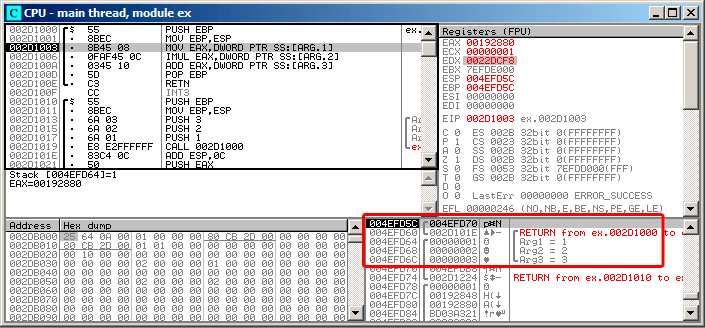
\includegraphics[scale=\FigScale]{patterns/05_passing_arguments/olly.png}
\caption{\olly: \RU{внутри функции}\EN{inside of} \ttf{}\EN{ function}}
\label{fig:passing_arguments_olly}
\end{figure}

\fi

\ifdefined\IncludeGCC
\subsection{GCC}

\RU{Скомпилируем то же в GCC 4.4.1 и посмотрим результат в \IDA:}
\EN{Let's compile the same in GCC 4.4.1 and see the results in \IDA:}

\lstinputlisting[caption=GCC 4.4.1]{patterns/05_passing_arguments/gcc.asm.\LANG}

\RU{Практически то же самое, если не считать мелких отличий описанных ранее.}
\EN{The result is almost the same with some minor differences discussed earlier.}

\RU{После вызова обоих функций \glslink{stack pointer}{указатель стека} не возвращается назад, 
потому что предпоследняя инструкция}
\EN{The \gls{stack pointer} is not set back after the two function calls(f and printf), 
because the penultimate} \TT{LEAVE} (\myref{x86_ins:LEAVE}) 
\RU{делает это за один раз, в конце исполнения.}
\EN{instruction takes care of this at the end.}
\fi

\section{x64}

\index{x86-64}
\RU{В x86-64 всё немного иначе, здесь аргументы функции (4 или 6) передаются через регистры, 
а \gls{callee} из читает их из регистров, а не из стека.}
\EN{The story is a bit different in x86-64. Function arguments (first 4 or first 6 of them) 
are passed in registers i.e. the \gls{callee} reads them from registers instead of reading them from the stack.}

\subsection{MSVC}

\Optimizing MSVC:

\lstinputlisting[caption=\Optimizing MSVC 2012 x64]{patterns/05_passing_arguments/x64_MSVC_Ox.asm.\LANG}

\RU{Как видно, очень компактная функция \ttf берет аргументы прямо из регистров.}
\EN{As we can see, the compact function \ttf takes all its arguments from the registers.}
\RU{Инструкция \LEA используется здесь для сложения чисел. 
Должно быть компилятор посчитал, что это будет эффективнее использования \TT{ADD}.}
\EN{The \LEA instruction here is used for addition,
apparently the compiler considered it faster than \TT{ADD}.}
\index{x86!\Instructions!LEA}
\RU{В самой \main{} \LEA{} также используется для подготовки первого и третьего аргумента: должно быть,
компилятор решил, что \LEA{} будет работать здесь быстрее, чем загрузка значения в регистр при помощи \MOV.}
\EN{\LEA is also used in the \main function to prepare the first and third \ttf arguments. The compiler
must have decided that this would work faster than the usual way of loading values into a register using \MOV instruction.}

\RU{Попробуем посмотреть вывод неоптимизирующего MSVC}\EN{Let's take a look at the non-optimizing MSVC output}:

\lstinputlisting[caption=MSVC 2012 x64]{patterns/05_passing_arguments/x64_MSVC_IDA.asm.\LANG}

\RU{Немного путаннее: все 3 аргумента из регистров зачем-то сохраняются в стеке.}
\EN{It looks somewhat puzzling because all 3 arguments from the registers are saved to the stack for some reason.}
\index{Shadow space}
\label{shadow_space}
\RU{Это называется}\EN{This is called} \q{shadow space}
\footnote{\href{http://go.yurichev.com/17256}{MSDN}}: 
\RU{каждая функция в Win64 может (хотя и не обязана) сохранять значения 4-х регистров там.}
\EN{every Win64 may (but is not required to) save all 4 register values there.}
\RU{Это делается по крайней мере из-за двух причин}\EN{This is done for two reasons}: 
1) \RU{в большой функции отвести целый регистр (а тем более 4 регистра) для входного аргумента 
слишком расточительно, так что к нему будет обращение через стек;}
\EN{it is too lavish to allocate a whole register (or even 4 registers) for an input argument,
so it will be accessed via stack;}
2) \RU{отладчик всегда знает, где найти аргументы функции в момент останова}\EN{the debugger is always
aware where to find the function arguments at a break}%
\footnote{\href{http://go.yurichev.com/17257}{MSDN}}.

\RU{Так что, какие-то большие функции могут сохранять входные аргументы в \q{shadows space} 
для использования в будущем, а небольшие функции, как наша, могут этого и не делать.}
\EN{So, some large functions can save their input arguments in the \q{shadows space} if they need to use them
during execution, but some small functions (like ours) may not do this.}

\RU{Место в стеке для \q{shadow space} выделяет именно \gls{caller}.}
\EN{It is a \gls{caller} responsibility to allocate \q{shadow space} in the stack.}

\ifdefined\IncludeGCC
\subsection{GCC}

\Optimizing GCC \RU{также делает понятный код}\EN{generates more or less understandable code}:

\lstinputlisting[caption=\Optimizing GCC 4.4.6 x64]{patterns/05_passing_arguments/x64_GCC_O3.s.\LANG}

\NonOptimizing GCC:

\lstinputlisting[caption=GCC 4.4.6 x64]{patterns/05_passing_arguments/x64_GCC.s.\LANG}

\index{Shadow space}
\RU{В соглашении о вызовах System V *NIX\cite{SysVABI} нет \q{shadow space}, но \gls{callee} тоже иногда
должен сохранять где-то аргументы, потому что, опять же, регистров может и не хватить на все действия.
Что мы здесь и видим.}
\EN{There are no \q{shadow space} requirements in System V *NIX\cite{SysVABI}, but the \gls{callee} may need to save
its arguments somewhere in case of registers shortage.}

\subsection{GCC: uint64\_t \RU{вместо}\EN{instead of} int}

\RU{Наш пример работал с 32-битным \Tint, поэтому использовались 32-битные части регистров с префиксом \TT{E-}.}
\EN{Our example works with 32-bit \Tint, that is why 32-bit register parts are used (prefixed by \TT{E-}).}

\RU{Его можно немного переделать, чтобы он заработал с 64-битными значениями}\EN{It can be altered slightly
in order to use 64-bit values}:

\lstinputlisting{patterns/05_passing_arguments/ex64.c}

\lstinputlisting[caption=\Optimizing GCC 4.4.6 x64]{patterns/05_passing_arguments/ex64_GCC_O3_IDA.asm.\LANG}

\RU{Собствено, всё то же самое, только используются регистры \IT{целиком}, с префиксом \TT{R-}.}
\EN{The code is the same, but this time the \IT{full size} registers (prefixed by \TT{R-}) are used.}
\fi

\ifdefined\IncludeARM
\section{ARM}

% subsections
\subsection{\NonOptimizingKeilVI (\ARMMode)}

\begin{lstlisting}
.text:000000A4 00 30 A0 E1                 MOV     R3, R0
.text:000000A8 93 21 20 E0                 MLA     R0, R3, R1, R2
.text:000000AC 1E FF 2F E1                 BX      LR
...
.text:000000B0             main
.text:000000B0 10 40 2D E9                 STMFD   SP!, {R4,LR}
.text:000000B4 03 20 A0 E3                 MOV     R2, #3
.text:000000B8 02 10 A0 E3                 MOV     R1, #2
.text:000000BC 01 00 A0 E3                 MOV     R0, #1
.text:000000C0 F7 FF FF EB                 BL      f
.text:000000C4 00 40 A0 E1                 MOV     R4, R0
.text:000000C8 04 10 A0 E1                 MOV     R1, R4
.text:000000CC 5A 0F 8F E2                 ADR     R0, aD_0        ; "%d\n"
.text:000000D0 E3 18 00 EB                 BL      __2printf
.text:000000D4 00 00 A0 E3                 MOV     R0, #0
.text:000000D8 10 80 BD E8                 LDMFD   SP!, {R4,PC}
\end{lstlisting}

\RU{В функции \main просто вызываются две функции, в первую (\ttf) передается три значения.}
\EN{The \main function simply calls two other functions, with three values passed to the 
first one~---(\ttf).}

\RU{Как уже было упомянуто, первые 4 значения в ARM обычно передаются в первых 4-х регистрах (\Reg{0}-\Reg{3}).}
\EN{As was noted before, in ARM the first 4 values are usually passed in the first 4 registers (\Reg{0}-\Reg{3}).}

\EN{The }\RU{Функция }\ttf\RU{, как видно, использует три первых регистра (\Reg{0}-\Reg{2}) как аргументы.}
\EN{function, as it seems, uses the first 3 registers (\Reg{0}-\Reg{2}) as arguments.}

\index{ARM!\Instructions!MLA}
\EN{The }\RU{Инструкция }\TT{MLA} (\IT{Multiply Accumulate}) \RU{перемножает два первых операнда (\Reg{3} и \Reg{1}), 
прибавляет к произведению
третий операнд (\Reg{2}) и помещает результат в нулевой регистр (\Reg{0}), через который, по стандарту, 
возвращаются значения функций.}
\EN{instruction multiplies its first two operands (\Reg{3} and \Reg{1}), adds the third operand (\Reg{2}) to the product and stores
the result into the zeroth register (\Reg{0}), via which, by standard, functions return values.}

\index{Fused multiply–add}
\RU{Умножение и сложение одновременно}\EN{Multiplication and addition at once}\footnote{\WPMAO} 
(\IT{Fused multiply–add}) \RU{это часто применяемая операция. Кстати, аналогичной
инструкции в x86 не было до появления FMA-инструкций в SIMD}%
\EN{is a very useful operation. By the way, there was no such instruction in x86 
before FMA-instructions appeared in SIMD}%
\footnote{\href{http://go.yurichev.com/17103}{wikipedia}}.

\RU{Самая первая инструкция}\EN{The very first} \TT{MOV R3, R0}, \RU{по-видимому, избыточна (можно было бы обойтись только одной инструкцией \TT{MLA}).}
\EN{instruction is, apparently, redundant (a single \TT{MLA} instruction could be used here instead).} 
\RU{Компилятор не оптимизировал её, ведь, это компиляция без оптимизации.}
\EN{The compiler has not optimized it, since this is non-optimizing compilation.}

\index{ARM!\RU{Переключение режимов}\EN{Mode switching}}
\index{ARM!\Instructions!BX}
\RU{Инструкция \TT{BX} возвращает управление по адресу, записанному в \ac{LR} и, если нужно, 
переключает режимы процессора с Thumb на ARM или наоборот.}
\EN{The \TT{BX} instruction returns the control to the address stored in the \ac{LR} register and, if necessary, 
switches the processor mode from Thumb to ARM or vice versa.}
\RU{Это может быть необходимым потому, что, как мы видим, 
функции \ttf неизвестно, из какого кода она будет вызываться, из ARM или Thumb.}
\EN{This can be necessary since, as we can see, function \ttf is not aware from what kind of code it may be
called, ARM or Thumb.}
\RU{Поэтому, если она будет вызываться из кода Thumb, \TT{BX} не только возвращает
управление в вызывающую функцию, но также переключает процессор в режим Thumb.}
\EN{Thus, if it gets called from Thumb code, 
\TT{BX} is not only returns control to the calling function,
but also switches the processor mode to Thumb.}
\RU{Либо не переключит, если функция вызывалась из кода для режима ARM: \cite[A2.3.2]{ARMref}.}
\EN{Or not switch, if the function was called from ARM code \cite[A2.3.2]{ARMref}.}
% look for "BXWritePC()" in manual

\subsection{\OptimizingKeilVI (\ARMMode)}

\begin{lstlisting}[label=ARM_leaf_example1]
.text:00000098             f
.text:00000098 91 20 20 E0                 MLA     R0, R1, R0, R2
.text:0000009C 1E FF 2F E1                 BX      LR
\end{lstlisting}

\index{ARM!\Instructions!MLA}
\RU{А вот и функция \ttf, скомпилированная компилятором Keil в режиме полной оптимизации}
\EN{And here is the \ttf function compiled by the Keil compiler in full optimization mode} (\Othree).
\RU{Инструкция \MOV была оптимизирована: теперь \TT{MLA} использует все входящие регистры 
и помещает результат в \Reg{0}, где вызываемая функция будет его читать и использовать.}
\EN{The \MOV instruction was optimized out (or reduced) and now \TT{MLA} uses all 
input registers and also places the result right into \Reg{0},
exactly where the calling function will read and use it.}

\subsection{\OptimizingKeilVI (\ThumbMode)}

\begin{lstlisting}[label=ARM_leaf_example2]
.text:0000005E 48 43                       MULS    R0, R1
.text:00000060 80 18                       ADDS    R0, R0, R2
.text:00000062 70 47                       BX      LR
\end{lstlisting}

\RU{В режиме Thumb инструкция \TT{MLA} недоступна, так что компилятору пришлось сгенерировать код, 
делающий обе операции по отдельности.}
\EN{The \TT{MLA} instruction is not available in Thumb mode, so the compiler generates the code doing these two 
operations (multiplication and addition) separately.}
\index{ARM!\Instructions!MULS}
\index{ARM!\Instructions!ADDS}
\RU{Первая инструкция \TT{MULS} умножает \Reg{0} на \Reg{1}, оставляя результат в \Reg{1}.}
\EN{First the \TT{MULS} instruction multiplies \Reg{0} by \Reg{1}, leaving the result in register \Reg{1}.}
\RU{Вторая (\TT{ADDS}) складывает результат и \Reg{2}, оставляя результат в \Reg{0}.}
\EN{The second instruction (\TT{ADDS}) adds the result and \Reg{2} leaving the result in register \Reg{0}.}

\subsection{ARM64}

\subsubsection{\Optimizing GCC (Linaro) 4.9}

\index{Fused multiply–add}
\index{ARM!\Instructions!MADD}
\RU{Тут всё просто}\EN{Everything here is simple}.
\EN{\TT{MADD} is just an instruction doing fused multiply/add (similar to the \TT{MLA} we already saw).}
\RU{\TT{MADD} это просто инструкция, производящая умножение и сложение одновременно (как \TT{MLA}, 
которую мы уже видели).}
\EN{All 3 arguments are passed in the 32-bit parts of X-registers.}
\RU{Все 3 аргумента передаются в 32-битных частях X-регистров.}
\EN{Indeed, the argument types are 32-bit \IT{int}'s.}
\RU{Действительно, типы аргументов это 32-битные \IT{int}'ы.}
\EN{The result is returned in \TT{W0}.}
\RU{Результат возвращается в \TT{W0}.}

\lstinputlisting[caption=\Optimizing GCC (Linaro) 4.9]{patterns/05_passing_arguments/ARM/ARM64_O3.s.\LANG}

\EN{Let's also extend all data types to 64-bit \TT{uint64\_t} and test:}%
\RU{Также расширим все типы данных до 64-битных \TT{uint64\_t} и попробуем:}

\lstinputlisting{patterns/05_passing_arguments/ex64.c}

\begin{lstlisting}
f:
	madd	x0, x0, x1, x2
	ret
main:
	mov	x1, 13396
	adrp	x0, .LC8
	stp	x29, x30, [sp, -16]!
	movk	x1, 0x27d0, lsl 16
	add	x0, x0, :lo12:.LC8
	movk	x1, 0x122, lsl 32
	add	x29, sp, 0
	movk	x1, 0x58be, lsl 48
	bl	printf
	mov	w0, 0
	ldp	x29, x30, [sp], 16
	ret

.LC8:
	.string	"%lld\n"
\end{lstlisting}

\EN{The \ttf{} function is the same, only the whole 64-bit X-registers are now used.}%
\RU{Функция \ttf{} точно такая же, только теперь используются полные части 64-битных X-регистров.}
\RU{Длинные 64-битные значения загружаются в регистры по частям, это описано здесь}%
\EN{Long 64-bit values are loaded into the registers by parts, this is also described here}: \myref{ARM_big_constants_loading}.

\subsubsection{\NonOptimizing GCC (Linaro) 4.9}

\EN{The non-optimizing compiler is more redundant:}
\RU{Неоптимизирующий компилятор выдает немного лишнего кода:}

\begin{lstlisting}
f:
	sub	sp, sp, #16
	str	w0, [sp,12]
	str	w1, [sp,8]
	str	w2, [sp,4]
	ldr	w1, [sp,12]
	ldr	w0, [sp,8]
	mul	w1, w1, w0
	ldr	w0, [sp,4]
	add	w0, w1, w0
	add	sp, sp, 16
	ret
\end{lstlisting}

\EN{The code saves its input arguments in the local stack, 
in case someone (or something) in this function needs using the \TT{W0...W2} 
registers. This prevents overwriting the original
function arguments, which may be needed again in the future.}
\RU{Код сохраняет входные аргументы в локальном стеке на случай если кому-то (или чему-то) в этой функции
понадобится использовать регистры \TT{W0...W2}, перезаписывая оригинальные аргументы функции, которые
могут понадобится в будущем.}
\RU{Это называется}\EN{This is called} \IT{Register Save Area.} \cite{ARM64_PCS}
\RU{Вызываемая функция не обязана сохранять их.}\EN{ The callee, however, is not obliged to save them.}
\RU{Это то же что и}\EN{This is somewhat similar to} \q{Shadow Space}: \myref{shadow_space}.

\RU{Почему оптимизирующий GCC 4.9 убрал этот, сохраняющий аргументы, код?}
\EN{Why did the optimizing GCC 4.9 drop this argument saving code?}
\EN{Because it did some additional optimizing work and concluded
that the function arguments will not be needed in the future 
and also that the registers \TT{W0...W2} will not be used.}
\RU{Потому что он провел дополнительную работу по оптимизации и сделал вывод, 
что аргументы функции не понадобятся в будущем и регистры \TT{W0...W2} также не будут использоваться.}

\index{ARM!\Instructions!MUL}
\index{ARM!\Instructions!ADD}
\RU{Также мы видим пару инструкций \TT{MUL}/\TT{ADD} вместо одной \TT{MADD}.}
\EN{We also see a \TT{MUL}/\TT{ADD} instruction pair instead of single a \TT{MADD}.}


\fi
\ifdefined\IncludeMIPS
\section{MIPS}

\lstinputlisting[caption=\Optimizing GCC 4.4.5]{patterns/05_passing_arguments/MIPS_O3_IDA.lst.\LANG}

\RU{Первые 4 аргумента функции передаются в четырех регистрах с префиксами A-.}
\EN{The first four function arguments are passed in four registers prefixed by A-.}

\index{MIPS!\Instructions!MULT}
\RU{В MIPS есть два специальных регистра: HI и LO, которые выставляются в 64-битный результат умножения
во время исполнения инструкции \TT{MULT}.}
\EN{There are two special registers in MIPS: HI and LO which are filled with the 64-bit result of the multiplication during the execution of the \TT{MULT} instruction.}
\index{MIPS!\Instructions!MFLO}
\index{MIPS!\Instructions!MFHI}
\RU{К регистрам можно обращаться только используя инструкции \TT{MFLO} и \TT{MFHI}.}
\EN{These registers are accessible only by using the \TT{MFLO} and \TT{MFHI} instructions.}
\RU{Здесь \TT{MFLO} берет младшую часть результата умножения и записывает в \$V0.}
\EN{\TT{MFLO} here takes the low-part of the multiplication result and stores it into \$V0.}
\RU{Так что старшая 32-битная часть результата игнорируется (содержимое регистра HI не используется).}
\EN{So the high 32-bit part of the multiplication result is dropped (the HI register content is not used).}
\RU{Действительно, мы ведь работаем с 32-битным типом \Tint.}
\EN{Indeed: we work with 32-bit \Tint data types here.}

\index{MIPS!\Instructions!ADDU}
\RU{И наконец, \TT{ADDU} (\q{Add Unsigned}~--- добавить беззнаковое) прибавляет значение третьего аргумента к результату.}
\EN{Finally, \TT{ADDU} (\q{Add Unsigned}) adds the value of the third argument to the result.}

\index{MIPS!\Instructions!ADD}
\index{MIPS!\Instructions!ADDU}
\index{Ada}
\index{Integer overflow}
\RU{В MIPS есть две разных инструкции сложения:}
\EN{There are two different addition instructions in MIPS:} \TT{ADD} \AndENRU \TT{ADDU}.
\RU{На самом деле, дело не в знаковых числах, а в исключениях: \TT{ADD} может вызвать исключение
во время переполнения. Это иногда полезно\footnote{\url{http://go.yurichev.com/17326}} и поддерживается,
например, в \ac{PL} Ada.}
\EN{The difference between them is not related to signedness, but to exceptions. \TT{ADD} can raise an exception on overflow, which is sometimes useful\footnote{\url{http://go.yurichev.com/17326}} and supported in Ada \ac{PL}, for instance.}
\TT{ADDU} \RU{не вызывает исключения во время переполнения}\EN{does not raise exceptions on overflow}.
\RU{А так как \CCpp не поддерживает всё это, мы видим здесь \TT{ADDU} вместо \TT{ADD}.}
\EN{Since \CCpp does not support this, in our example we see \TT{ADDU} instead of \TT{ADD}.}

\RU{32-битный результат оставляется в}\EN{The 32-bit result is left in} \$V0.

\index{MIPS!\Instructions!JAL}
\index{MIPS!\Instructions!JALR}
\RU{В \main есть новая для нас инструкция:}
\EN{There is a new instruction for us in \main:} \TT{JAL} (\q{Jump and Link}). 
\RU{Разница между JAL и JALR в том, что относительное смещение кодируется в первой инструкции,
а JALR переходит по абсолютному адресу, записанному в регистр (\q{Jump and Link Register}).}
\EN{The difference between JAL and JALR is that a relative offset is encoded in the first instruction, 
while JALR jumps to the absolute address stored in a register (\q{Jump and Link Register}).}
\RU{Обе функции \ttf и \main расположены в одном объектном файле, так что относительный адрес
\ttf известен и фиксирован.}
\EN{Both \ttf and \main functions are located in the same object file, so the relative address of \ttf 
is known and fixed.}

\fi

\chapter{\RU{Ещё о возвращаемых результатах}\EN{More about results returning}}

\index{x86!\Registers!EAX}
\RU{Результат выполнения функции в x86 обычно возвращается}%
\EN{In x86, the result of function execution is usually returned}%
\footnote{\Seealso: 
MSDN: Return Values (C++): \href{http://go.yurichev.com/17258}{MSDN}}
\RU{через регистр \EAX, 
а если результат имеет тип байт или символ (\Tchar), 
то в самой младшей части \EAX~--- \AL. Если функция возвращает число с плавающей запятой, 
то будет использован регистр FPU \ST{0}.
\ifdefined\IncludeARM
\index{ARM!\Registers!R0}
В ARM обычно результат возвращается в регистре \Reg{0}.
\fi
}
\EN{in the \EAX register. 
If it is byte type or a character (\Tchar), then the lowest part of register \EAX (\AL) is used. 
If a function returns a \Tfloat number, the FPU register \ST{0} is used instead.
\ifdefined\IncludeARM
\index{ARM!\Registers!R0}
In ARM, the result is usually returned in the \Reg{0} register.
\fi
}

\section{\RU{Попытка использовать результат функции возвращающей \Tvoid}
\EN{Attempt to use the result of a function returning \Tvoid}}

\RU{Кстати, что будет, если возвращаемое значение в функции \main объявлять не как \Tint, а как \Tvoid?}
\EN{So, what if the \main function return value was declared of type \Tvoid and not \Tint?}

\RU{Т.н. startup-код вызывает \main примерно так:}
\EN{The so-called startup-code is calling \main roughly as follows:}

\begin{lstlisting}
push envp
push argv
push argc
call main
push eax
call exit
\end{lstlisting}

\RU{Иными словами:}\EN{In other words:}

\begin{lstlisting}
exit(main(argc,argv,envp));
\end{lstlisting}

\RU{Если вы объявите \main как \Tvoid, и ничего не будете возвращать явно (при помощи выражения \IT{return}), 
то в единственный аргумент exit() попадет
то, что лежало в регистре \EAX на момент выхода из \main.}
\EN{If you declare \main as \Tvoid, nothing is to be returned explicitly 
(using the \IT{return} statement),
then something random, that was stored in the \EAX register at the end of \main becomes 
the sole argument of the exit() function.}
\RU{Там, скорее всего, будет какие-то случайное число, оставшееся от работы вашей функции.
Так что код завершения программы будет псевдослучайным.}
\EN{Most likely, there will be a random value, left from your function execution,
so the exit code of program is pseudorandom.}\PTBRph{}\ESph{}\PLph{} \\

\RU{Мы можем это проиллюстрировать}\EN{We can illustrate this fact}. 
\RU{Заметьте, что у функции}\EN{Please note that here the} \main
\RU{тип возвращаемого значения именно}\EN{function has a} \Tvoid\EN{ return type}:

\begin{lstlisting}
#include <stdio.h>

void main()
{
	printf ("Hello, world!\n");
};
\end{lstlisting}

\RU{Скомпилируем в}\EN{Let's compile it in} Linux.

\index{puts() \RU{вместо}\EN{instead of} printf()}
GCC 4.8.1 \RU{заменила}\EN{replaced} \printf \RU{на}\EN{with} \puts 
\ifx\LITE\undefined
(\RU{мы видели это прежде}\EN{we have seen this before}: \myref{puts})
\fi
, \RU{но это нормально, потому что}\EN{but that's OK, since} \puts \RU{возвращает количество
выведенных символов, так же как и}\EN{returns the number of characters printed out, just like} \printf.
\RU{Обратите внимание на то, что}\EN{Please notice that} \EAX \RU{не обнуляется перед выходом их}\EN{is not 
zeroed before} \main\EN{'s end}.
\RU{Это значит что \EAX перед выходом из \main содержит то, что \puts оставляет там.}
\EN{This implies that the value of \EAX at the end of \main contains what \puts has left there.}

\begin{lstlisting}[caption=GCC 4.8.1]
.LC0:
	.string	"Hello, world!"
main:
	push	ebp
	mov	ebp, esp
	and	esp, -16
	sub	esp, 16
	mov	DWORD PTR [esp], OFFSET FLAT:.LC0
	call	puts
	leave
	ret
\end{lstlisting}

\index{bash}
\RU{Напишем небольшой скрипт на bash, показывающий статус возврата (\q{exit status} или \q{exit code})}
\EN{Let' s write a bash script that shows the exit status}:

\begin{lstlisting}[caption=tst.sh]
#!/bin/sh
./hello_world
echo $?
\end{lstlisting}

\RU{И запустим}\EN{And run it}:

\begin{lstlisting}
$ tst.sh 
Hello, world!
14
\end{lstlisting}

14 \RU{это как раз количество выведенных символов}\EN{is the number of characters printed}.

\section{\RU{Что если не использовать результат функции?}\EN{What if we do not use the function result?}}

\RU{\printf возвращает количество успешно выведенных символов, но результат работы этой функции 
редко используется на практике.}
\EN{\printf returns the count of characters successfully output, but the result of this function 
is rarely used in practice.}
\RU{Можно даже явно вызывать функции, чей смысл именно в возвращаемых значениях, но явно не использовать их:}
\EN{It is also possible to call a function whose essence is in returning a value, and not use it:}

\begin{lstlisting}
int f()
{
    // skip first 3 random values
    rand();
    rand();
    rand();
    // and use 4th
    return rand();
};
\end{lstlisting}

\EN{The result of the rand() function is left in \EAX, in all four cases.}
\RU{Результат работы rand() остается в \EAX во всех четырех случаях.}
\EN{But in the first 3 cases, the value in \EAX is just thrown away.}
\RU{Но в первых трех случаях значение, лежащее в \EAX, просто выбрасывается.}

\ifx\LITE\undefined
\section{\RU{Возврат структуры}\EN{Returning a structure}}

\index{\CLanguageElements!return}
\RU{Вернемся к тому факту, что возвращаемое значение остается в регистре \EAX.}
\EN{Let's go back to the fact that the return value is left in the \EAX register.}
\RU{Вот почему старые компиляторы Си не способны создавать функции, возвращающие нечто большее, нежели 
помещается 
в один регистр (обычно тип \Tint), а когда нужно, приходится возвращать через указатели, указываемые 
в аргументах.}
\EN{That is why old C compilers cannot create functions capable of returning something that does not fit in one 
register (usually \Tint), but if one needs it, one have to return information via pointers passed 
as function's arguments.}
\RU{Так что как правило, если функция должна вернуть несколько значений, она возвращает только одно, 
а остальные~--- через указатели.}
\EN{So, usually, if a function needs to return several values, it returns only one, and 
all the rest---via pointers.}
\RU{Хотя позже и стало возможным, вернуть, скажем, целую структуру, но этот метод до сих пор не 
очень популярен. 
Если функция должна вернуть структуру, вызывающая функция должна сама, скрыто и прозрачно для программиста, 
выделить место и передать указатель на него в качестве первого аргумента. Это почти то же самое 
что и сделать это вручную, но компилятор прячет это.}
\EN{Now it has become possible to return, let's say, an entire structure, but that is still not very popular. 
If a function has to return a large structure, the \gls{caller} must allocate it and pass a pointer to it via the first argument, transparently for the programmer. 
That is almost the same as to pass a pointer in the first argument manually, but the compiler hides it.}

\RU{Небольшой пример:}\EN{Small example:}

\lstinputlisting{patterns/06_return_results/6_1.c}

\dots \RU{получим}\EN{what we got} (MSVC 2010 \Ox):

\lstinputlisting{patterns/06_return_results/6_1.asm}

\RU{\TT{\$T3853} это имя внутреннего макроса для передачи указателя на структуру.}
\EN{The macro name for internal passing of pointer to a structure here is \TT{\$T3853}.}

\index{\CLanguageElements!C99}
\RU{Этот пример можно даже переписать, используя расширения C99}\EN{This example can be rewritten using
the C99 language extensions}:

\lstinputlisting{patterns/06_return_results/6_1_C99.c}

\lstinputlisting[caption=GCC 4.8.1]{patterns/06_return_results/6_1_C99.asm}

\RU{Как видно, функция просто заполняет поля в структуре, выделенной вызывающей функцией. 
Как если бы передавался просто указатель на структуру.
Так что никаких проблем с эффективностью нет.}
\EN{As we see, the function is just filling the structure's fields allocated by
the caller function,
as if a pointer to the structure was passed.
So there are no performance drawbacks.}
\fi

\ifx\LITE\undefined
\chapter{\RU{Указатели}\EN{Pointers}}
\index{\CLanguageElements!\Pointers}
\label{label_pointers}

\RU{Указатели также часто используются для возврата значений из функции (вспомните случай
со \scanf{}~(\myref{label_scanf})).}
\EN{Pointers are often used to return values from functions (recall \scanf case~(\myref{label_scanf})).}
\RU{Например, когда функции нужно вернуть сразу два значения.}
\EN{For example, when a function needs to return two values.}

\section{\RU{Пример с глобальными переменными}\EN{Global variables example}}

\lstinputlisting{patterns/061_pointers/global.c}

\RU{Это компилируется в}\EN{This compiles to}:

\lstinputlisting[caption=\Optimizing MSVC 2010 (/Ob0)]{patterns/061_pointers/global.asm}

\index{\olly}
\clearpage
\RU{Посмотрим это в}\EN{Let's see this in} \olly:

\begin{figure}[H]
\centering
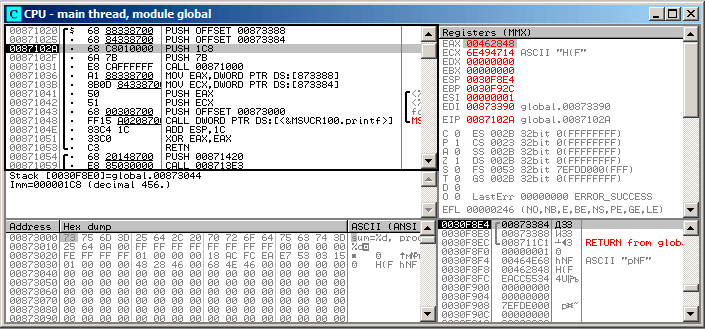
\includegraphics[scale=\FigScale]{patterns/061_pointers/olly_global1.png}
\caption{\olly: \RU{передаются адреса двух глобальных переменных в}
\EN{global variables addresses are passed to} \ttfone}
\label{fig:pointers_olly_global_1}
\end{figure}

\RU{В начале адреса обоих глобальных переменных передаются в}\EN{First, global
variables' addresses are passed to} \ttfone.
\RU{Можно нажать}\EN{We can click} \q{Follow in dump} 
\RU{на элементе стека и в окне слева 
увидим место в сегменте данных, выделенное для двух переменных.}
\EN{on the stack element, and we can see the place in the data segment allocated 
for the two variables.}
\RU{Эти переменные обнулены, потому что по стандарту неинициализированные данные (\ac{BSS}) 
обнуляются перед началом исполнения: \cite[6.7.8p10]{C99TC3}.}

\clearpage
\EN{These variables are zeroed, because non-initialized data (from \ac{BSS}) is cleared before
the execution begins: \cite[6.7.8p10]{C99TC3}.}
\RU{И они находятся в сегменте данных, о чем можно удостовериться, нажав}
\EN{They reside in the data segment, we can verify this by pressing} Alt-M \RU{и увидев карту
памяти}\EN{and reviewing the memory map}:

\begin{figure}[H]
\centering
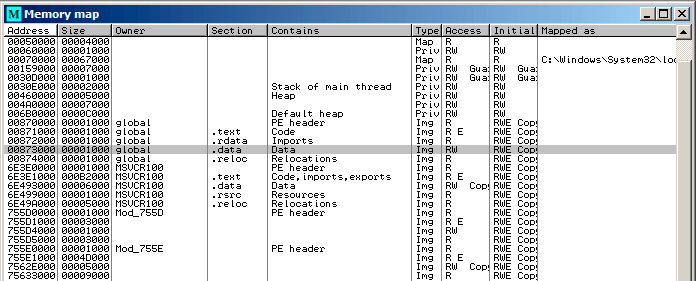
\includegraphics[scale=\FigScale]{patterns/061_pointers/olly_global5.png}
\caption{\olly: \RU{карта памяти}\EN{memory map}}
\label{fig:pointers_olly_global_5}
\end{figure}

\clearpage
\RU{Трассируем}\EN{Let's trace} (F7) \RU{до начала исполнения}\EN{to the start of} \ttfone: 

\begin{figure}[H]
\centering
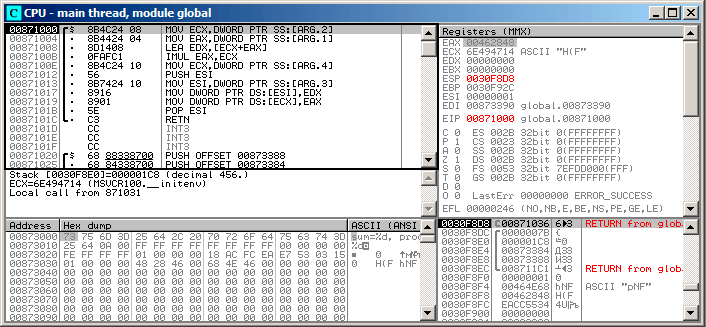
\includegraphics[scale=\FigScale]{patterns/061_pointers/olly_global2.png}
\caption{\olly: \RU{начало работы \ttfone}\EN{\ttfone starts}}
\label{fig:pointers_olly_global_2}
\end{figure}

\RU{В стеке видны значения}\EN{Two values are visible in the stack} 456 (\TT{0x1C8}) \AndENRU 
123 (\TT{0x7B}), \RU{а также адреса двух глобальных переменных}\EN{and also the addresses of the two global variables}.

\clearpage
\RU{Трассируем до конца}\EN{Let's trace until the end of} \ttfone.
\RU{Мы видим в окне слева, как результаты вычисления появились в глобальных переменных}%
\EN{In the left bottom window we see how the results of the calculation appear in the global variables}: 

\begin{figure}[H]
\centering
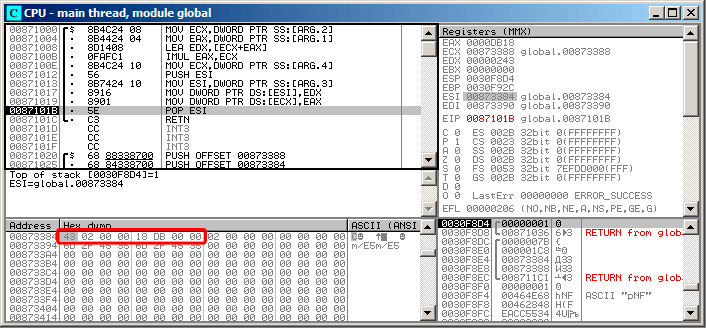
\includegraphics[scale=\FigScale]{patterns/061_pointers/olly_global3.png}
\caption{\olly: \ttfone \RU{заканчивает работу}\EN{execution completed}}
\label{fig:pointers_olly_global_3}
\end{figure}

\clearpage
\RU{Теперь из глобальных переменных значения загружаются в регистры для передачи в}
\EN{Now the global variables' values are loaded into registers ready for passing to} \printf \EN{(via the stack)}:

\begin{figure}[H]
\centering
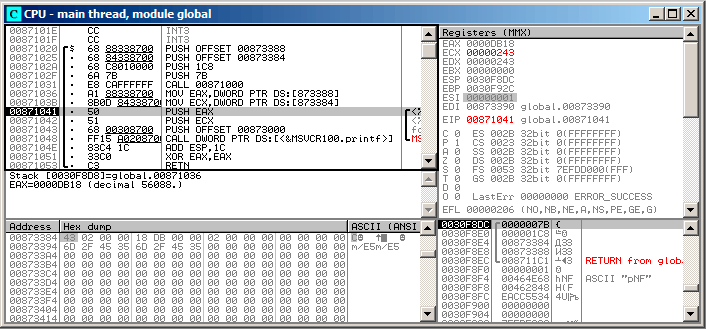
\includegraphics[scale=\FigScale]{patterns/061_pointers/olly_global4.png}
\caption{\olly: \RU{адреса глобальных переменных передаются в}
\EN{global variables' addresses are passed into} \printf}
\label{fig:pointers_olly_global_4}
\end{figure}

\section{\RU{Пример с локальными переменными}\EN{Local variables example}}

\RU{Немного переделаем пример}\EN{Let's rework our example slightly}:

\lstinputlisting[caption=\RU{теперь переменные локальные}
\EN{now the \TT{sum} and \TT{product} variables are local}]{patterns/061_pointers/local.c.\LANG}

\RU{Код функции }\ttfone \RU{не изменится}\EN{code will not change}.
\RU{Изменится только \main}\EN{Only the code of \main will do}:

\lstinputlisting[caption=\Optimizing MSVC 2010 (/Ob0)]{patterns/061_pointers/local.asm}

\newcommand{\PtrsAddresses}{\TT{0x2EF854} \AndENRU \TT{0x2EF858}\xspace}

\clearpage
\RU{Снова посмотрим в}\EN{Let's look again with} \olly.
\RU{Адреса локальных переменных в стеке это}\EN{The addresses of the local variables in the stack are} \PtrsAddresses.
\RU{Видно, как они заталкиваются в стек}\EN{We see how these are pushed into the stack}: 

\begin{figure}[H]
\centering
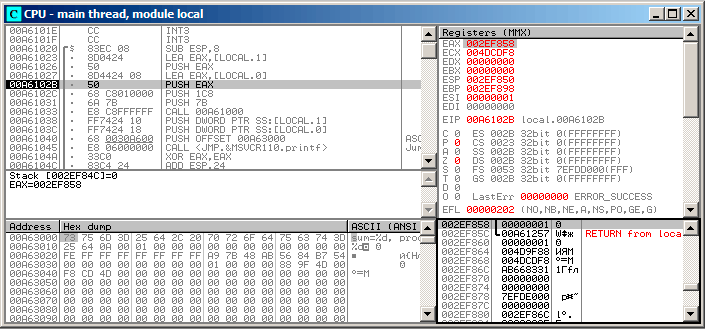
\includegraphics[scale=\FigScale]{patterns/061_pointers/olly_stk1.png}
\caption{\olly: \RU{адреса локальных переменных заталкиваются в стек}\EN{local variables' addresses are
pushed into the stack}}
\label{fig:pointers_olly_stk_1}
\end{figure}

\clearpage
\RU{Начало работы \ttfone}\EN{\ttfone starts}.
\RU{В стеке по адресам}\EN{So far there is only random garbage in the stack at} \PtrsAddresses \RU{пока находится случайный мусор}:

\begin{figure}[H]
\centering
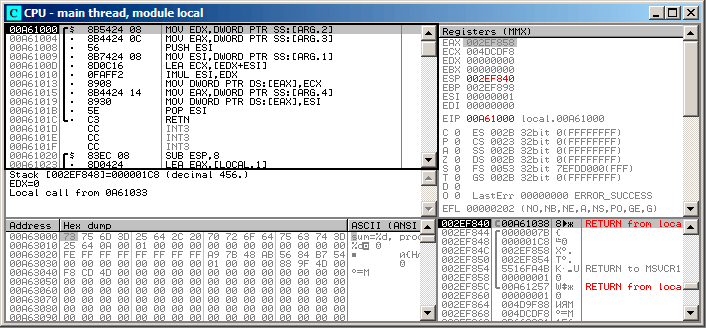
\includegraphics[scale=\FigScale]{patterns/061_pointers/olly_stk2.png}
\caption{\olly: \ttfone \RU{начинает работу}\EN{starting}}
\label{fig:pointers_olly_stk_2}
\end{figure}

\clearpage
\RU{Конец работы \ttfone}\EN{\ttfone completes}:

\begin{figure}[H]
\centering
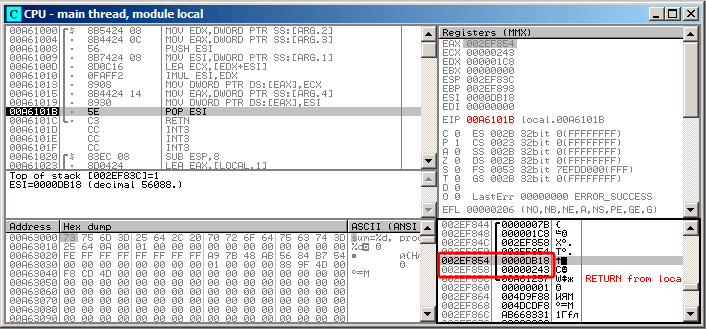
\includegraphics[scale=\FigScale]{patterns/061_pointers/olly_stk3.png}
\caption{\olly: \ttfone \RU{заканчивает работу}\EN{completes execution}}
\label{fig:pointers_olly_stk_3}
\end{figure}

\RU{В стеке по адресам \PtrsAddresses теперь находятся значения \TT{0xDB18} \AndENRU \TT{0x243}, 
это результаты работы \ttfone.}
\EN{We now find \TT{0xDB18} \AndENRU \TT{0x243} at addresses \PtrsAddresses. These values are
the \ttfone results.}

\section{\Conclusion{}}

\RU{\ttfone может одинаково хорошо возвращать результаты работы в любые места памяти.} 
\EN{\ttfone could return pointers to any place in memory, located anywhere.}
\RU{В этом суть и удобство указателей.}
\EN{This is in essence the usefulness of the pointers.}

\RU{Кстати,}\EN{By the way, \Cpp} \IT{references} \RU{в \Cpp работают точно так же}\EN{work exactly the
same way}. \RU{Читайте больше об этом}\EN{Read more about them}: (\myref{cpp_references}).

\fi
\chapter{\RU{Оператор GOTO}\EN{GOTO operator}}

\RU{Оператор GOTO считается анти-паттерном}\EN{The GOTO operator is generally considered as anti-pattern.} 
\cite{Dijkstra:1968:LEG:362929.362947}, 
\RU{но тем не менее, его можно использовать в разумных пределах}
\EN{Nevertheless, it can be used reasonably} \cite{Knuth:1974:SPG:356635.356640}, \cite[1.3.2]{CBook}.

\RU{Вот простейший пример}\EN{Here is a very simple example}:

\lstinputlisting{patterns/065_GOTO/goto.c}

\RU{Вот что мы получаем в}\EN{Here is what we have got in} MSVC 2012:

\lstinputlisting[caption=MSVC 2012]{patterns/065_GOTO/MSVC_goto.asm}

\RU{Выражение \IT{goto} заменяется инструкцией \JMP, которая работает точно также:
безусловный переход в другое место.}
\EN{The \IT{goto} statement has been simply replaced by a \JMP instruction, which has the same
effect: unconditional jump to another place.}

\RU{Вызов второго \printf может исполнится только при помощи человеческого вмешательства,
используя отладчик или модифицирование кода.}
\EN{The second \printf could be executed only with human intervention, 
by using a debugger or by patching the code.}
\PTBRph{}\ESph{}\PLph{}\\
\\
\ifdefined\IncludeHiew
\clearpage
\RU{Это также может быть простым упражнением на модификацию кода.}
\EN{This could also be useful as a simple patching exercise.}
\RU{Откроем исполняемый файл в}\EN{Let's open the resulting executable in} Hiew:

\begin{figure}[H]
\centering
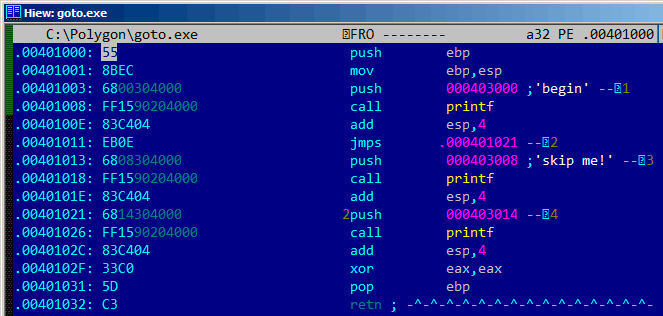
\includegraphics[scale=\FigScale]{patterns/065_GOTO/hiew1.png}
\caption{Hiew}
\label{fig:goto_hiew1}
\end{figure}

\clearpage
\RU{Поместите курсор по адресу}\EN{Place the cursor to address} \JMP (\TT{0x410}), 
\RU{нажмите}\EN{press} F3 (\RU{редактирование}\EN{edit}), \RU{нажмите два нуля, так что
опкод становится}\EN{press zero twice, so the opcode becomes} \TT{EB 00}:

\begin{figure}[H]
\centering
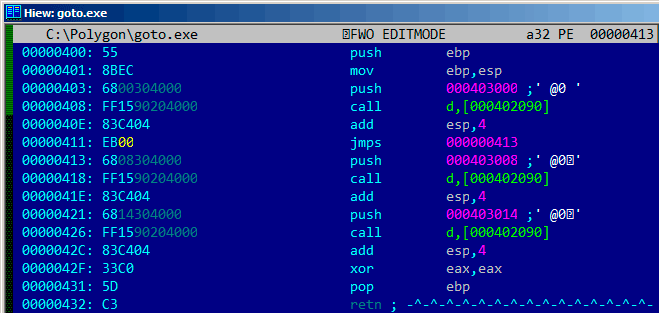
\includegraphics[scale=\FigScale]{patterns/065_GOTO/hiew2.png}
\caption{Hiew}
\label{fig:goto_hiew2}
\end{figure}

\RU{Второй байт опкода \JMP это относительное смещение от перехода. 0 означает место
прямо после текущей инструкции.}
\EN{The second byte of the \JMP opcode denotes the relative offset for the jump, 0 means the point
right after the current instruction.}
\RU{Теперь \JMP не будет пропускать следующий вызов \printf.}
\EN{So now \JMP not skipping the second \printf call.}

\RU{Нажмите F9 (запись) и выйдите.}
\EN{Press F9 (save) and exit.}
\RU{Теперь мы запускаем исполняемый файл и видим это}\EN{Now if we run the executable we should see 
this}:

\begin{figure}[H]
\centering
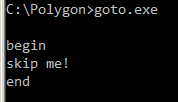
\includegraphics[scale=\NormalScale]{patterns/065_GOTO/result.png}
\caption{\RU{Результат}\EN{Patched executable output}}
\label{fig:goto_result}
\end{figure}

\RU{Подобного же эффекта можно достичь, если заменить инструкцию \JMP на две инструкции \NOP.}
\EN{The same result could be achieved by replacing the \JMP instruction with 2 \NOP instructions.}
\RU{\NOP имеет опкод \TT{0x90} и длину в 1 байт, так что нужно 2 инструкции для замены.}
\EN{\NOP has an opcode of \TT{0x90} and length of 1 byte, so we need 2 instructions as \JMP replacement (which is 2 bytes in size).}
\fi

\section{\RU{Мертвый код}\EN{Dead code}}

\RU{Вызов второго \printf также называется \q{мертвым кодом} (\q{dead code}) 
в терминах компиляторов.}
\EN{The second \printf call is also called \q{dead code} in compiler terms.}
\RU{Это значит, что он никогда не будет исполнен.}
\EN{This means that the code will never be executed.}
\EN{So when you compile this example with optimizations, the compiler removes \q{dead code}, leaving
no trace of it:}
\RU{Так что если вы компилируете этот пример с оптимизацией, компилятор удаляет \q{мертвый
код} не оставляя следа:}

\lstinputlisting[caption=\Optimizing MSVC 2012]{patterns/065_GOTO/MSVC_goto_Ox.asm}

\RU{Впрочем, строку}\EN{However, the compiler forgot to remove the} \q{skip me!} \RU{компилятор 
убрать забыл}\EN{string}.

%Note: cl "/Ox" option for maximum optimisation does get rid of "skip me" string as well

\ifdefined\IncludeExercises
\section{\Exercise}

% TODO debugger example can fit here
\RU{Попробуйте добиться того же самого в вашем любимом компиляторе и отладчике.}
\EN{Try to achieve the same result using your favorite compiler and debugger.}
\fi

\chapter{\RU{Условные переходы}\EN{Conditional jumps}}
\label{sec:Jcc}
\index{\CLanguageElements!if}

% sections
\section{\RU{Простой пример}\EN{Simple example}}

\lstinputlisting{patterns/07_jcc/simple/ex.c}

% subsections
\subsection{x86}

\subsubsection{x86 + MSVC}

\RU{Имеем в итоге функцию \TT{f\_signed()}:}\EN{Here is how the \TT{f\_signed()} function looks like:}

\lstinputlisting[caption=\NonOptimizing MSVC 2010]{patterns/07_jcc/simple/signed_MSVC.asm}

\index{x86!\Instructions!JLE}
\RU{Первая инструкция \JLE значит}
\EN{The first instruction, \JLE, stands for} \IT{Jump if Less or Equal}. 
\RU{Если второй операнд больше первого или 
равен ему, произойдет переход туда, где будет следующая проверка.}
\EN{In other words, if the second operand is 
larger or equal to the first one, the control flow will be passed to the specified in the instruction address or label.}
\RU{А если это условие не срабатывает (то есть второй операнд меньше первого), то перехода не будет, 
и сработает первый \printf.}
\EN{If this condition does not trigger because the second operand is smaller than the first one, the control flow would not be altered and the first \printf would be executed.}
\index{x86!\Instructions!JNE}
\RU{Вторая проверка это}\EN{The second check is} \JNE: \IT{Jump if Not Equal}.
\RU{Переход не произойдет, если операнды равны}\EN{The control flow will not change if the operands are 
equal}.

\index{x86!\Instructions!JGE}
\RU{Третья проверка}\EN{The third check is} \JGE: \IT{Jump if Greater or Equal}\EMDASH{}\RU{переход 
если первый операнд больше второго или равен ему}\EN{jump if the first operand is larger than 
the second or if they are equal}.
\RU{Кстати, если все три условных перехода сработают, ни один \printf не вызовется. 
Но без внешнего вмешательства это невозможно.}
\EN{So, if all three conditional jumps are triggered, none of the \printf calls would be executed whatsoever. 
This is impossible without special intervention.}

\EN{Now let's take a look at the \TT{f\_unsigned()} function.}
\EN{The}\RU{Функция} \TT{f\_unsigned()} \RU{точно такая же, за тем исключением, что используются инструкции 
\JBE и \JAE вместо \JLE и \JGE:}
\EN{function is the same as \TT{f\_signed()}, with the exception that the \JBE and \JAE instructions
are used instead of \JLE and \JGE, as follows:}

\lstinputlisting[caption=GCC]{patterns/07_jcc/simple/unsigned_MSVC.asm}

\index{x86!\Instructions!JBE}
\index{x86!\Instructions!JAE}
\RU{Здесь всё то же самое, только инструкции условных переходов немного другие:}
\EN{As already mentioned, the branch instructions are different:}
\JBE\EMDASH{}\IT{Jump if Below or Equal} \AndENRU \JAE\EMDASH{}\IT{Jump if Above or Equal}.
\RU{Эти инструкции}\EN{These instructions} (\JA/\JAE/\JB/\JBE) 
\RU{отличаются от}\EN{differ from} \JG/\JGE/\JL/\JLE \RU{тем, что работают с беззнаковыми переменными.}
\EN{in the fact that they work with unsigned numbers.}

\index{x86!\Instructions!JA}
\index{x86!\Instructions!JB}
\index{x86!\Instructions!JG}
\index{x86!\Instructions!JL}
\index{Signed numbers}
\RU{Отступление: смотрите также секцию о представлении знака в числах}
\EN{See also the section about signed number representations}~(\myref{sec:signednumbers}).
\RU{Таким образом, увидев где используется \JG/\JL вместо \JA/\JB и наоборот, 
можно сказать почти уверенно насчет того, 
является ли тип переменной знаковым (signed) или беззнаковым (unsigned).}
\EN{That is why if we see \JG/\JL in use instead of \JA/\JB or vice-versa, 
we can be almost sure that the variables are signed or unsigned, respectively.}

\RU{Далее функция \main, где ничего нового для нас нет:}
\EN{Here is also the \main function, where there is nothing much new to us:}

\lstinputlisting[caption=\main]{patterns/07_jcc/simple/main_MSVC.asm}

\ifdefined\IncludeOlly
\input{patterns/07_jcc/simple/olly.tex}
\fi

\clearpage
\subsubsection{x86 + MSVC + Hiew}
\index{Hiew}

\RU{Можем попробовать модифицировать исполняемый файл так,}\EN{We can try to patch the executable file in a way} 
\RU{чтобы функция}\EN{that the} \TT{f\_unsigned()} \RU{всегда показывала}\EN{function would always print} \q{a==b}, 
\RU{при любых входящих значениях}\EN{no matter the input values}.
\RU{Вот как она выглядит в}\EN{Here is how it looks in} Hiew:

\begin{figure}[H]
\centering
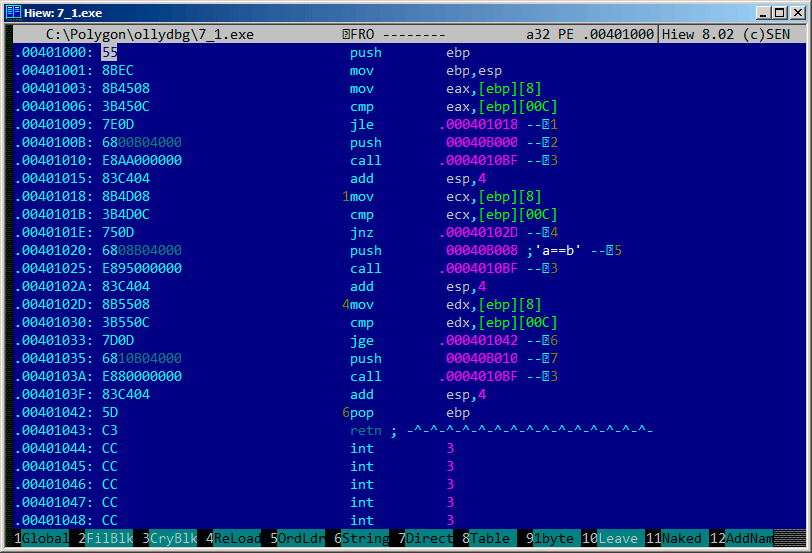
\includegraphics[scale=\FigScale]{patterns/07_jcc/simple/hiew_unsigned1.png}
\caption{Hiew: \RU{функция }\TT{f\_unsigned()}\EN{ function}}
\label{fig:jcc_hiew_1}
\end{figure}

\RU{Собственно, задач три}\EN{Essentially, we need to accomplish three tasks}:
\begin{itemize}
\item \RU{заставить первый переход срабатывать всегда}\EN{force the first jump to always trigger};
\item \RU{заставить второй переход не срабатывать никогда}\EN{force the second jump to never trigger};
\item \RU{заставить третий переход срабатывать всегда}\EN{force the third jump to always trigger}.
\end{itemize}

\RU{Так мы направим путь исполнения кода (code flow) во второй}\EN{Thus we can direct the code flow
to always pass through the second} \printf,
\RU{и он всегда будет срабатывать и выводить на консоль}\EN{and output} \q{a==b}.

\RU{Для этого нужно изменить три инструкции (или байта)}\EN{Three instructions (or bytes) has to be patched}:

\begin{itemize}
\item \RU{Первый переход теперь будет}\EN{The first jump becomes} \JMP, \RU{но смещение перехода 
(\gls{jump offset}) останется прежним}\EN{but the \gls{jump offset} would remain the same}.

\item \RU{Второй переход может быть и будет срабатывать иногда, но в любом случае он будет совершать переход
только на следующую инструкцию, потому что мы выставляем смещение перехода (\gls{jump offset}) в 0.}
\EN{The second jump might be triggered sometimes, but in any case it will jump to the next
instruction, because, we set the \gls{jump offset} to 0.}
\RU{В этих инструкциях смещение перехода просто прибавляется к адресу следующей инструкции.}
\EN{In these instructions the \gls{jump offset} is added to the address for the next instruction.}
\RU{Когда смещение 0, переход будет на следующую инструкцию.}\EN{So if the offset is 0,
the jump will transfer the control to the next instruction.}

\item \RU{Третий переход конвертируем в \JMP точно так же, как и первый, он будет срабатывать всегда.}
\EN{The third jump we replace with \JMP just as we do with the first one, so it will always trigger.}

\end{itemize}

\clearpage
\RU{Что и делаем}\EN{Here is the modified code}:

\begin{figure}[H]
\centering
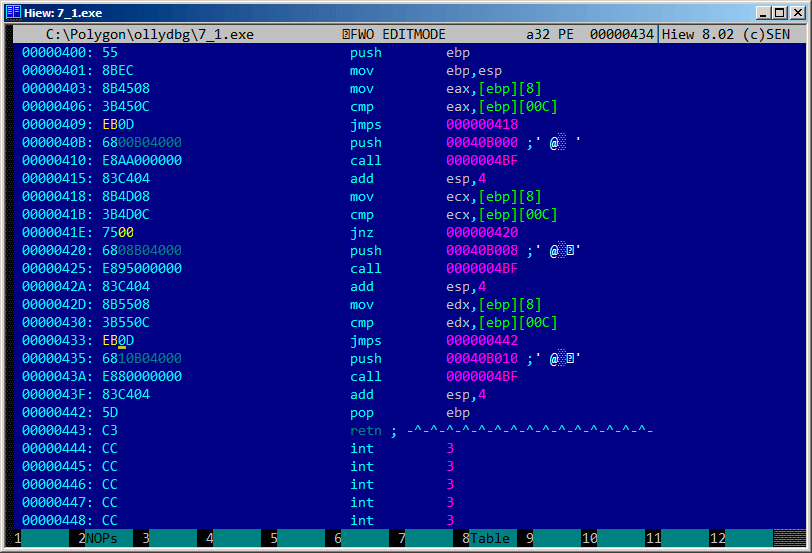
\includegraphics[scale=\FigScale]{patterns/07_jcc/simple/hiew_unsigned2.png}
\caption{Hiew: \RU{модифицируем функцию}\EN{let's modify the} \TT{f\_unsigned()}\EN{ function}}
\label{fig:jcc_hiew_2}
\end{figure}

\RU{Если забыть про какой-то из переходов, то тогда будет срабатывать несколько вызовов \printf, 
а нам ведь нужно чтобы исполнялся только один.}
\EN{If we miss to change any of these jumps, then several \printf calls may execute, while we want to execute only one.}

\ifdefined\IncludeGCC
\subsubsection{\NonOptimizing GCC}

\index{puts() \RU{вместо}\EN{instead of} printf()}
\NonOptimizing GCC 4.4.1 \RU{производит почти такой же код, за исключением}
\EN{produces almost the same code, but with} \puts~(\myref{puts}) \RU{вместо}\EN{instead of} \printf.

\subsubsection{\Optimizing GCC}

\RU{Наблюдательный читатель может спросить, зачем исполнять \CMP так много раз,
если флаги всегда одни и те же}\EN{An observant reader may ask, why execute \CMP several times, 
if the flags has the same values after each execution}?
\RU{По видимому, оптимизирующий MSVC не может этого делать, но GCC 4.8.1 делает больше оптимизаций:}
\EN{Perhaps optimizing MSVC can not do this, but optimizing GCC 4.8.1 can go deeper:}

\lstinputlisting[caption=GCC 4.8.1 f\_signed()]{patterns/07_jcc/simple/GCC_O3_signed.asm}

% should be here instead of 'switch' section?
\RU{Мы здесь также видим}\EN{We also see} \TT{JMP puts} \RU{вместо}\EN{here instead of} \TT{CALL puts / RETN}.
\RU{Этот прием описан немного позже}%
\EN{This kind of trick will have explained later}: \myref{JMP_instead_of_RET}.

\RU{Нужно сказать, что x86-код такого типа редок}\EN{This type of x86 code 
is somewhat rare}.
MSVC 2012\RU{, как видно, не может генерировать подобное}\EN{ as it seems, can't generate such code}.
\RU{С другой стороны, программисты на ассемблере прекрасно осведомлены о том, что инструкции}\EN{On the other hand, assembly language programmers are fully aware of the fact that} \TT{Jcc} \RU{можно располагать последовательно.}
\EN{instructions can be stacked.}
\RU{Так что если вы видите это где-то, имеется немалая вероятность, что этот фрагмент кода был написан вручную.}
\EN{So if you see such stacking somewhere, it is highly probable that the code was hand-written.}

\EN{The}\RU{Функция} \TT{f\_unsigned()} \RU{получилась не настолько эстетически короткой}\EN{function is not that 
\ae{}sthetically short}:

\lstinputlisting[caption=GCC 4.8.1 f\_unsigned()]{patterns/07_jcc/simple/GCC_O3_unsigned.asm.\LANG}

\RU{Тем не менее, здесь 2 инструкции \TT{CMP} вместо трех.}
\EN{Nevertheless, there are two \TT{CMP} instructions instead of three.}
\RU{Так что, алгоритмы оптимизации GCC 4.8.1, наверное, ещё пока не идеальны.}
\EN{So optimization algorithms of GCC 4.8.1 are probably not perfect yet.} 
\fi

\ifdefined\IncludeARM
\subsection{ARM}

% subsubsections here
\input{patterns/07_jcc/simple/ARM/ARM32}
\input{patterns/07_jcc/simple/ARM/ARM64}

\fi
\ifdefined\IncludeMIPS
\subsection{MIPS}

\RU{Одна отличительная особенность MIPS это отсутствие регистра флагов.}
\EN{One distinctive MIPS feature is the absence of flags.}
\RU{Очевидно, так было сделано для упрощения анализа зависимости данных (data dependency).}
\EN{Apparently, it was done to simplify the analysis of data dependencies.}

\index{x86!\Instructions!SETcc}
\index{MIPS!\Instructions!SLT}
\index{MIPS!\Instructions!SLTU}
\RU{Так что здесь есть инструкция, похожая на SETcc в x86: SLT (\q{Set on Less Than}~--- установить если
меньше чем, знаковая версия) и SLTU (беззнаковая версия).}
\EN{There are instructions similar to SETcc in x86: SLT (\q{Set on Less Than}: signed version) and 
SLTU (unsigned version).}
\RU{Эта инструкция устанавливает регистр-получатель в 1 если условие верно или в 0 в противном случае.}
\EN{These instructions sets destination register value to 1 if the condition is true or to 0 if otherwise.}

\index{MIPS!\Instructions!BEQ}
\index{MIPS!\Instructions!BNE}
\RU{Затем регистр-получатель проверяется, используя инструкцию 
BEQ (\q{Branch on Equal} --- переход если равно) или BNE (\q{Branch on Not Equal} --- переход если не равно) 
и может произойти переход.}
\EN{The destination register is then checked using BEQ (\q{Branch on Equal}) or BNE (\q{Branch on Not Equal}) 
and a jump may occur.}

\RU{Так что эта пара инструкций должна использоваться в MIPS для сравнения и перехода.}
\EN{So, this instruction pair has to be used in MIPS for comparison and branch.}

\RU{Начнем с знаковой версии нашей функции:}
\EN{Let's first start with the signed version of our function:}

\lstinputlisting[caption=\NonOptimizing GCC 4.4.5 (IDA)]{patterns/07_jcc/simple/O0_MIPS_signed_IDA.lst.\LANG}

\q{SLT REG0, REG0, REG1} \RU{сокращается в IDA до более короткой формы}\EN{is reduced by IDA to its 
shorter form} \q{SLT REG0, REG1}.
\index{MIPS!\Pseudoinstructions!BEQZ}
\RU{Мы также видим здесь псевдоинструкцию BEQZ (\q{Branch if Equal to Zero}~--- переход если равно нулю), 
которая, на самом деле, \q{BEQ REG, \$ZERO, LABEL}.}
\EN{We also see there BEQZ pseudoinstruction (\q{Branch if Equal to Zero}), 
which are in fact \q{BEQ REG, \$ZERO, LABEL}.}

\index{MIPS!\Instructions!SLTU}
\RU{Беззнаковая версия точно такая же, только здесь используется SLTU (беззнаковая версия, 
отсюда \q{U} в названии) вместо SLT:}
\EN{The unsigned version is just the same, but SLTU (unsigned version, hence \q{U} in name) is used instead of SLT:}

\lstinputlisting[caption=\NonOptimizing GCC 4.4.5 (IDA)]{patterns/07_jcc/simple/O0_MIPS_unsigned_IDA.lst}

\fi

\section{\RU{Вычисление абсолютной величины}\EN{Calculating absolute value}}
\label{sec:abs}

\RU{Это простая функция}\EN{A simple function}:

\lstinputlisting{abs.c}

\subsection{\Optimizing MSVC}

\RU{Обычный способ генерации кода:}
\EN{This is how the code is usually generated:}

\lstinputlisting[caption=\Optimizing MSVC 2012 x64]{patterns/07_jcc/abs/abs_MSVC2012_Ox_x64.asm.\LANG}

\ifdefined\IncludeGCC
\RU{GCC 4.9 делает почти то же самое.}
\EN{GCC 4.9 does mostly the same.}
\fi

\ifdefined\IncludeARM
\subsection{\OptimizingKeilVI: \ThumbMode}

\lstinputlisting[caption=\OptimizingKeilVI: \ThumbMode]{patterns/07_jcc/abs/abs_Keil_thumb_O3.s.\LANG}

\index{ARM!\Instructions!RSB}
\RU{В ARM нет инструкции для изменения знака, так что компилятор Keil использует инструкцию \q{Reverse Subtract},
которая просто вычитает, но с операндами, переставленными наоборот.}
\EN{ARM lacks a negate instruction, so the Keil compiler uses the \q{Reverse Subtract} instruction, which just subtracts with reversed operands.}

\subsection{\OptimizingKeilVI: \ARMMode}

\RU{В режиме ARM можно добавлять коды условий к некоторым инструкций, что компилятор Keil и сделал:}
\EN{It is possible to add condition codes to some instructions in ARM mode, so that is what the Keil compiler does:}

\lstinputlisting[caption=\OptimizingKeilVI: \ARMMode]{patterns/07_jcc/abs/abs_Keil_ARM_O3.s.\LANG}

\RU{Теперь здесь нет условных переходов и это хорошо:}
\EN{Now there are no conditional jumps and this is good:} 
\myref{branch_predictors}.

\subsection{\NonOptimizing GCC 4.9 (ARM64)}

\index{ARM!\Instructions!XOR}
\RU{В ARM64 есть инструкция NEG для смены знака:}
\EN{ARM64 has instruction NEG for negating:}

\lstinputlisting[caption=\Optimizing GCC 4.9 (ARM64)]{patterns/07_jcc/abs/abs_GCC49_ARM64_O0.s.\LANG}
\fi

\ifdefined\IncludeMIPS
\subsection{MIPS}

\lstinputlisting[caption=\Optimizing GCC 4.4.5 (IDA)]{patterns/07_jcc/abs/MIPS_O3_IDA.lst.\LANG}

\index{MIPS!\Instructions!BLTZ}
\RU{Видим здесь новую инструкцию}\EN{Here we see a new instruction}: BLTZ (\q{Branch if Less Than Zero}).
\index{MIPS!\Instructions!SUBU}
\index{MIPS!\Pseudoinstructions!NEGU}
\RU{Тут есть также псевдоинструкция NEGU, которая на самом деле вычитает из нуля.}
\EN{There is also the NEGU pseudoinstruction, which just does subtraction from zero.}
\RU{Суффикс \q{U} в обоих инструкциях SUBU и NEGU означает, что при целочисленном переполнении исключение не
сработает.}
\EN{The \q{U} suffix in both SUBU and NEGU implies that no exception to be raised in case of integer overflow.}

\fi

\ifx\LITE\undefined
\subsection{\RU{Версия без переходов}\EN{Branchless version}?}

\RU{Возможна также версия и без переходов, мы рассмотрим её позже:}
\EN{You could have also a branchless version of this code. This we will review later:} \myref{chap:branchless_abs}.
\fi

\section{\RU{Тернарный условный оператор}\EN{Ternary conditional operator}}
\label{chap:cond}

\RU{Тернарный условный оператор (ternary conditional operator) в}\EN{The ternary conditional operator in} \CCpp \RU{это}\EN{has the following syntax}:

\begin{lstlisting}
expression ? expression : expression
\end{lstlisting}

\RU{И вот пример}\EN{Here is an example}:

\lstinputlisting{patterns/07_jcc/cond_operator/cond.c}

\subsection{x86}

\RU{Старые и неоптимизирующие компиляторы генерируют код так, как если бы выражение \TT{if/else} было использовано
вместо него:}
\EN{Old and non-optimizing compilers generate assembly code just as if an \TT{if/else} statement was used:}

\lstinputlisting[caption=\NonOptimizing MSVC 2008]{patterns/07_jcc/cond_operator/MSVC2008.asm.\LANG}

\lstinputlisting[caption=\Optimizing MSVC 2008]{patterns/07_jcc/cond_operator/MSVC2008_Ox.asm.\LANG}

\RU{Новые компиляторы могут быть более краткими}\EN{Newer compilers are more concise}:

\lstinputlisting[caption=\Optimizing MSVC 2012 x64]{patterns/07_jcc/cond_operator/MSVC2012_Ox_x64.asm.\LANG}

\index{x86!\Instructions!CMOVcc}
\Optimizing GCC 4.8 \ForENRU x86 \RU{также использует инструкцию}\EN{also uses the} \TT{CMOVcc}\RU{, тогда как
неоптимизирующий GCC 4.8 использует условные переходы}\EN{ instruction, while the non-optimizing GCC 4.8 uses conditional jumps}.

\ifdefined\IncludeARM
\subsection{ARM}

\index{x86!\Instructions!ADRcc}
\Optimizing Keil \ForENRU \RU{режима ARM также использует инструкцию \TT{ADRcc}, срабатывающую при некотором
условии}\EN{ARM mode also uses the conditional instructions \TT{ADRcc}}:

\lstinputlisting[label=cond_Keil_ARM_O3,caption=\OptimizingKeilVI (\ARMMode)]{patterns/07_jcc/cond_operator/Keil_ARM_O3.s.\LANG}

\RU{Без внешнего вмешательства инструкции \TT{ADREQ} и \TT{ADRNE} никогда не исполнятся одновременно.}
\EN{Without manual intervention, the two instructions \TT{ADREQ} and \TT{ADRNE} cannot be executed in the same run.}

\Optimizing Keil \ForENRU \RU{режима Thumb вынужден использовать инструкции условного перехода, потому
что тут нет инструкции загрузки значения, поддерживающей флаги условия}\EN{Thumb mode needs to use 
conditional jump instructions, since there are no load instructions
that support conditional flags}:

\lstinputlisting[caption=\OptimizingKeilVI (\ThumbMode)]{patterns/07_jcc/cond_operator/Keil_thumb_O3.s.\LANG}

\subsection{ARM64}

\Optimizing GCC (Linaro) 4.9 \ForENRU ARM64 \RU{также использует условные переходы}\EN{also uses conditional jumps}:

\lstinputlisting[label=cond_ARM64,caption=\Optimizing GCC (Linaro) 4.9]{patterns/07_jcc/cond_operator/ARM64_GCC_O3.s.\LANG}

\RU{Это потому что в ARM64 нет простой инструкции загрузки с флагами условия, как \TT{ADRcc} в 32-битном 
режиме ARM или \TT{CMOVcc} в x86}
\EN{That is because ARM64 does not have a simple load instruction with conditional flags, like \TT{ADRcc} in 32-bit ARM mode or CMOVcc in x86}
\cite[p390, C5.5]{ARM64ref}.
\index{ARM!\Instructions!CSEL}
\RU{Но с другой стороны, там есть инструкция \TT{CSEL} (\q{Conditional SELect}), но GCC 4.9 наверное, пока не так
хорош, чтобы генерировать её в таком фрагменте кода.}
\EN{It has, however, \q{Conditional SELect} instruction (\TT{CSEL}), but GCC 4.9 does not seem to be smart enough to use it in such piece of code.}
\fi

\ifdefined\IncludeMIPS
\subsection{MIPS}

\RU{GCC 4.4.5 для MIPS тоже не так хорош, к сожалению}\EN{Unfortunately, GCC 4.4.5 for MIPS is not very smart, either}:

\lstinputlisting[caption=\Optimizing GCC 4.4.5 (\assemblyOutput)]{patterns/07_jcc/cond_operator/MIPS_O3.s.\LANG}

\fi

\subsection{\RU{Перепишем, используя обычный \TT{if/else}}\EN{Let's rewrite it in an \TT{if/else} way}}

\lstinputlisting{patterns/07_jcc/cond_operator/cond2.c}

\index{x86!\Instructions!CMOVcc}
\RU{Интересно, оптимизирующий GCC 4.8 для x86 также может генерировать \TT{CMOVcc} в этом случае:}
\EN{Interestingly, optimizing GCC 4.8 for x86 was also able to use \TT{CMOVcc} in this case:}

\lstinputlisting[caption=\Optimizing GCC 4.8]{patterns/07_jcc/cond_operator/cond2_GCC_O3.s.\LANG}

\ifdefined\IncludeARM
\Optimizing Keil \InENRU \RU{режиме ARM генерирует код идентичный этому:}\EN{ARM mode generates 
code identical to} \lstref{cond_Keil_ARM_O3}.
\fi

\RU{Но оптимизирующий}\EN{But the optimizing} MSVC 2012 \RU{пока не так хорош}\EN{is not that good (yet)}.

\ifx\LITE\undefined
\subsection{\Conclusion{}}

\RU{Почему оптимизирующие компиляторы стараются избавиться от условных переходов? Читайте больше об этом здесь:}
\EN{Why optimizing compilers try to get rid of conditional jumps? Read here about it:} \myref{branch_predictors}.
\fi

\section{\RU{Поиск минимального и максимального значения}\EN{Getting minimal and maximal values}}

\subsection{32-bit}

\lstinputlisting{patterns/07_jcc/minmax/minmax.c}

\lstinputlisting[caption=\NonOptimizing MSVC 2013]{patterns/07_jcc/minmax/minmax_MSVC_2013.asm.\LANG}

\index{x86!\Instructions!Jcc}
\RU{Эти две функции отличаются друг от друга только инструкцией условного перехода:
JGE (\q{Jump if Greater or Equal}~--- переход если больше или равно) используется в первой
и JLE (\q{Jump if Less or Equal}~--- переход если меньше или равно) во второй.}
\EN{These two functions differ only in the conditional jump instruction: 
JGE (\q{Jump if Greater or Equal}) is used in the first one
and JLE (\q{Jump if Less or Equal}) in the second.}

\index{\CompilerAnomaly}
\label{MSVC_double_JMP_anomaly}
\RU{Здесь есть ненужная инструкция \JMP в каждой функции, которую MSVC, наверное, оставил по ошибке.}
\EN{There is one unneeded \JMP instruction in each function, which MSVC probably left by mistake.}

\ifx\LITE\undefined
\subsubsection{\RU{Без переходов}\EN{Branchless}}

\RU{ARM в режиме Thumb напоминает нам x86-код:}
\EN{ARM for Thumb mode reminds us of x86 code:}

\lstinputlisting[caption=\OptimizingKeilVI (\ThumbMode)]{patterns/07_jcc/minmax/minmax_Keil_Thumb_O3.s.\LANG}

\index{ARM!\Instructions!Bcc}
\RU{Функции отличаются только инструкцией перехода: BGT и BLT.}
\EN{The functions differ in the branching instruction: BGT and BLT.}

\RU{А в режиме ARM можно использовать условные суффиксы, так что код более плотный.}
\EN{It's possible to use conditional suffixes in ARM mode, so the code is shorter.}
\RU{MOVcc будет исполнена только если условие верно:}
\EN{MOVcc is to be executed only if the condition is met:}
\index{ARM!\Instructions!MOVcc}

\lstinputlisting[caption=\OptimizingKeilVI (\ARMMode)]{patterns/07_jcc/minmax/minmax_Keil_ARM_O3.s.\LANG}

\index{x86!\Instructions!CMOVcc}
\Optimizing GCC 4.8.1 \RU{и оптимизирующий}\EN{and optimizing} MSVC 2013 
\RU{могут использовать инструкцию CMOVcc, которая аналогична MOVcc в ARM:}
\EN{can use CMOVcc instruction, which is analogous to MOVcc in ARM:}

\lstinputlisting[caption=\Optimizing MSVC 2013]{patterns/07_jcc/minmax/minmax_GCC481_O3.s.\LANG}

\subsection{64-bit}

\lstinputlisting{patterns/07_jcc/minmax/minmax64.c}

\RU{Тут есть ненужные перетасовки значений, но код в целом понятен:}
\EN{There is some unneeded value shuffling, but the code is comprehensible:}

\lstinputlisting[caption=\NonOptimizing GCC 4.9.1 ARM64]{patterns/07_jcc/minmax/minmax64_GCC_49_ARM64_O0.s}

\subsubsection{\RU{Без переходов}\EN{Branchless}}

\RU{Нет нужды загружать аргументы функции из стека, они уже в регистрах:}
\EN{No need to load function arguments from the stack, as they are already in the registers:}

\lstinputlisting[caption=\Optimizing GCC 4.9.1 x64]{patterns/07_jcc/minmax/minmax64_GCC_49_x64_O3.s.\LANG}

MSVC 2013 \RU{делает то же самое}\EN{does almost the same}.

\index{ARM!\Instructions!CSEL}
\RU{В ARM64 есть инструкция CSEL, которая работает точно также, как и MOVcc в ARM и CMOVcc в x86, но название
другое:}
\EN{ARM64 has the CSEL instruction, which works just as MOVcc in ARM or CMOVcc in x86, just the name is different:}
\q{Conditional SELect}.

\lstinputlisting[caption=\Optimizing GCC 4.9.1 ARM64]{patterns/07_jcc/minmax/minmax64_GCC_49_ARM64_O3.s.\LANG}

\ifdefined\IncludeMIPS
\subsection{MIPS}

\RU{А GCC 4.4.5 для MIPS не так хорош, к сожалению}\EN{Unfortunately, GCC 4.4.5 for MIPS is not that good}:

\lstinputlisting[caption=\Optimizing GCC 4.4.5 (IDA)]{patterns/07_jcc/minmax/minmax_MIPS_O3_IDA.lst.\LANG}

\RU{Не забывайте о \IT{branch delay slots}: первая MOVE исполняется \IT{перед} BEQZ,
вторая MOVE исполняется только если переход не произошел.}
\EN{Do not forget about the \IT{branch delay slots}: the first MOVE is executed \IT{before} BEQZ, 
the second MOVE is executed only if the branch wasn't taken.}

\fi
\fi


\section{\Conclusion{}}

\subsection{x86}

\RU{Примерный скелет условных переходов}\EN{Here's the rough skeleton of a conditional jump}:

\lstinputlisting[caption=x86]{patterns/07_jcc/skel1.lst.\LANG}

\ifdefined\IncludeARM

\subsection{ARM}

\lstinputlisting[caption=ARM]{patterns/07_jcc/skel2.lst.\LANG}
\fi

\ifdefined\IncludeMIPS

\subsection{MIPS}

\begin{lstlisting}[caption=\RU{Проверка на ноль}\EN{Check for zero}]
BEQZ REG, label
...
\end{lstlisting}

\begin{lstlisting}[caption=\RU{Меньше ли нуля?}\EN{Check for less than zero:}]
BLTZ REG, label
...
\end{lstlisting}

\begin{lstlisting}[caption=\RU{Проверка на равенство}\EN{Check for equal values}]
BEQ REG1, REG2, label
...
\end{lstlisting}

\begin{lstlisting}[caption=\RU{Проверка на неравенство}\EN{Check for non-equal values}]
BNE REG1, REG2, label
...
\end{lstlisting}

\begin{lstlisting}[caption=\RU{Проверка на меньше, больше (знаковое)}\EN{Check for less than, greater than (signed)}]
SLT REG1, REG2, REG3
BEQ REG1, label
...
\end{lstlisting}

\begin{lstlisting}[caption=\RU{Проверка на меньше, больше (беззнаковое)}\EN{Check for less than, greater than (unsigned)}]
SLTU REG1, REG2, REG3
BEQ REG1, label
...
\end{lstlisting}
\fi

\subsection{\RU{Без инструкций перехода}\EN{Branchless}}

\index{ARM!\Instructions!MOVcc}
\index{x86!\Instructions!CMOVcc}
\index{ARM!\Instructions!CSEL}
\EN{If the body of a condition statement is very short, the conditional move instruction can be used: 
MOVcc in ARM (in ARM mode), CSEL in ARM64, CMOVcc in x86.}
\RU{Если тело условного выражения очень короткое, может быть
использована инструкция условного копирования: MOVcc в ARM (в режиме ARM), CSEL в ARM64, CMOVcc в x86.}

\ifdefined\IncludeARM
\subsubsection{ARM}

\RU{В режиме ARM можно использовать условные суффиксы для некоторых инструкций:}
\EN{It's possible to use conditional suffixes in ARM mode for some instructions:}

\lstinputlisting[caption=ARM (\ARMMode)]{patterns/07_jcc/skel4.lst.\LANG}

\RU{Нет никаких ограничений на количество инструкций с условными суффиксами до тех пор,
пока флаги CPU не были модифицированы одной из таких инструкций.}
\EN{Of course, there is no limit for the number of instructions with conditional code suffixes, 
as long as the CPU flags are not modified by any of them.}
% FIXME: list of such instructions or \myref{} to it

\index{ARM!\Instructions!IT}
\RU{В режиме Thumb есть инструкция IT, позволяющая дополнить следующие 4 инструкции суффиксами, задающими
условие.}
\EN{Thumb mode has the IT instruction, allowing to add conditional suffixes to the next four instructions.}
\RU{Читайте больше об этом}\EN{Read more about it}: \myref{ARM_Thumb_IT}.

\lstinputlisting[caption=ARM (\ThumbMode)]{patterns/07_jcc/skel3.lst.\LANG}
\fi

\ifdefined\IncludeExercises
\section{\Exercise}

(ARM64) \RU{Попробуйте переписать код в}\EN{Try rewriting the code in} \lstref{cond_ARM64} 
\RU{убрав все инструкции условного перехода, и используйте инструкцию \TT{CSEL}}\EN{by removing all 
conditional jump instructions and using the \TT{CSEL} instruction}.
\fi


\chapter{\SwitchCaseDefaultSectionName}
\index{\CLanguageElements!switch}

% sections
\section{\RU{Если вариантов мало}\EN{Small number of cases}}

\lstinputlisting{patterns/08_switch/1_few/few.c}

\subsection{x86}

\subsubsection{\NonOptimizing MSVC}

\RU{Это дает в итоге}\EN{Result} (MSVC 2010):

\lstinputlisting[caption=MSVC 2010]{patterns/08_switch/1_few/few_msvc.asm}

\RU{Наша функция со оператором switch(), с небольшим количеством вариантов, 
это практически аналог подобной конструкции:}
\EN{Our function with a few cases in switch() is in fact analogous to this construction:}

\lstinputlisting[label=switch_few_ifelse]{patterns/08_switch/1_few/few_analogue.c}

\index{\CLanguageElements!switch}
\index{\CLanguageElements!if}
\RU{Когда вариантов немного и мы видим подобный код, невозможно сказать с уверенностью, был ли
в оригинальном исходном коде switch(), либо просто набор операторов if().}
\EN{If we work with switch() with a few cases it is impossible to be sure if it was
a real switch() in the source code, or just a pack of if() statements.}
\index{\SyntacticSugar}
\RU{То есть, switch() это синтаксический сахар для большого количества вложенных проверок 
при помощи if().}
\EN{This implies that switch() is like syntactic sugar for a large number of nested if()s.}

\RU{В самом выходном коде ничего особо нового, 
за исключением того, что компилятор зачем-то 
перекладывает входящую переменную ($a$) во временную в локальном стеке \TT{v64}%
\footnote{Локальные переменные в стеке с префиксом \TT{tv}~--- 
так MSVC называет внутренние переменные для своих нужд}.}
\EN{There is nothing especially new to us in the generated code,
with the exception of the compiler moving 
input variable 
$a$ to a temporary local variable \TT{tv64}
\footnote{Local variables in stack are prefixed with \TT{tv}---%
that's how MSVC names internal variables for its needs}.}

\RU{Если скомпилировать это при помощи GCC 4.4.1, то будет почти то же самое, даже с максимальной оптимизацией 
(ключ \Othree).}
\EN{If we compile this in GCC 4.4.1, we'll get almost the same result, even with maximal optimization
turned on (\Othree option).}

\subsubsection{\Optimizing MSVC}

\RU{Попробуем включить оптимизацию кодегенератора}%
% TODO separate various kinds of \TT
% idea: enclose command lines in a specific environment, like \cmdline{} 
% assembly instructions in \asm{} (now both \TT and \q{} are used),
% variables in,  like \var{}
% messages (string constants) in something else, like \strconst
% to separate them all. Now they all use \TT, which is not best
% \INS{} for all instructions including operands? --DY
\EN{Now let's turn on optimization in} MSVC (\Ox): \TT{cl 1.c /Fa1.asm /Ox}

\label{JMP_instead_of_RET}
\lstinputlisting[caption=MSVC]{patterns/08_switch/1_few/few_msvc_Ox.asm}

\RU{Вот здесь уже всё немного по-другому, причем не без грязных трюков.}
\EN{Here we can see some dirty hacks.}

\index{x86!\Instructions!JZ}
\index{x86!\Instructions!JE}
\index{x86!\Instructions!SUB}
\RU{Первое: \TT{а} помещается в \EAX и от него отнимается 0. Звучит абсурдно, но нужно это для того, чтобы проверить, 
0 ли в \EAX был до этого? Если да, то выставится флаг \ZF (что означает, что результат вычитания 0 от числа 
стал 0) и первый условный переход \JE (\IT{Jump if Equal} или его синоним \JZ~--- \IT{Jump if Zero}) 
сработает на метку \TT{\$LN4@f}, где выводится сообщение \TT{'zero'}.
Если первый переход не сработал, от значения отнимается по единице, 
и если на какой-то стадии в результате образуется 0, то сработает соответствующий переход.}
\EN{First: the value of $a$ is placed in \EAX and 0 is subtracted from it. Sounds absurd, but it is done to check if 
the value in \EAX was 0. If yes, the \ZF flag is to be set (e.g. subtracting from 0 is 0) 
and the first conditional jump \JE (\IT{Jump if Equal} or synonym \JZ~---\IT{Jump if Zero}) is to be triggered 
and control flow is to be passed to the \TT{\$LN4@f} label, where the \TT{'zero'} message is being printed. 
If the first jump doesn't get triggered, 1 is subtracted from the input value and if at some stage the result is 0, 
the corresponding jump is to be triggered.}

\RU{И в конце концов, если ни один из условных переходов не сработал, управление передается \printf
со строковым аргументом \TT{'something unknown'}.}
\EN{And if no jump gets triggered at all, the control flow passes to \printf with string argument \TT{'something unknown'}.}

\label{jump_to_last_printf}
\index{\Stack}
\RU{Второе: мы видим две, мягко говоря, необычные вещи: указатель на сообщение помещается в переменную $a$, 
и затем \printf вызывается не через \CALL, а через \JMP. Объяснение этому простое. 
Вызывающая функция заталкивает в стек некоторое значение и через \CALL вызывает нашу функцию. 
\CALL в свою очередь заталкивает в стек адрес возврата (\ac{RA}) и делает безусловный переход на адрес нашей функции. 
Наша функция в самом начале (да и в любом её месте, потому что в теле функции нет ни одной инструкции, 
которая меняет что-то в стеке или в \ESP) имеет следующую разметку стека:}
\EN{Second: we see something unusual for us: a string pointer is placed into the $a$ variable, and 
then \printf is called not via \CALL, but via \JMP. There is a simple explanation for that: 
the \gls{caller} pushes a value to the stack and calls our function via \CALL. 
\CALL itself pushes the return address (\ac{RA}) to the stack and does an unconditional jump to our function address. 
Our function at any point of execution (since it do not contain any instruction that moves the stack 
pointer) has the following stack layout:}

\begin{itemize}
\item\ESP\EMDASH\RU{хранится}\EN{points to} \ac{RA}
\item\TT{ESP+4}\EMDASH\RU{хранится значение $a$}\EN{points to the $a$ variable} 
\end{itemize}

\RU{С другой стороны, чтобы вызвать \printf, нам нужна почти такая же разметка стека, 
только в первом аргументе нужен указатель на строку. Что, собственно, этот код и делает.}
\EN{On the other side, when we need to call \printf here we need exactly the same stack 
layout, except for the first \printf argument, which needs to point to the string. 
And that is what our code does.}

\RU{Он заменяет свой первый аргумент на адрес строки, и затем передает управление \printf, как если бы вызвали не 
нашу функцию \ttf, а сразу \printf. 
\printf выводит некую строку на \gls{stdout}, затем исполняет инструкцию \RET, 
которая из стека достает \ac{RA} и управление передается в ту функцию, 
которая вызывала \ttf, минуя при этом конец функции \ttf.}
\EN{It replaces the function's first argument with the address of the string and 
jumps to \printf, as if we didn't call our function \ttf, but directly \printf.
\printf prints a string to \gls{stdout} and then executes the \RET instruction, which POPs 
\ac{RA} from the stack and control flow is returned not to \ttf but rather to \ttf's \gls{callee}, 
bypassing the end of the \ttf function.}

\index{\CStandardLibrary!longjmp()}
\newcommand{\URLSJ}{\href{http://go.yurichev.com/17121}{wikipedia}}
\RU{Всё это возможно, потому что \printf вызывается в \ttf в самом конце. 
Всё это чем-то даже похоже на \TT{longjmp()}\footnote{\URLSJ}.
И всё это, разумеется, сделано для экономии времени исполнения.}
\EN{All this is possible because \printf is called right at the end of the \ttf function in all cases. 
In some way, it is similar to the \TT{longjmp()}\footnote{\URLSJ} function.
And of course, it is all done for the sake of speed.}

\ifdefined\IncludeARM
\RU{Похожая ситуация с компилятором для ARM описана в секции}
\EN{A similar case with the ARM compiler is described in} \q{\PrintfSeveralArgumentsSectionName}%
\EN{section, here}~(\myref{ARM_B_to_printf}).
\fi

\ifdefined\IncludeOlly
\input{patterns/08_switch/1_few/olly.tex}
\fi

\ifdefined\IncludeARM
\subsection{ARM: \OptimizingKeilVI (\ARMMode)}
\index{\CLanguageElements!switch}

\lstinputlisting{patterns/08_switch/1_few/few_ARM_ARM_O3.asm}

\RU{Мы снова не сможем сказать, глядя на этот код, был ли в оригинальном исходном коде switch() 
либо же несколько операторов if().}
\EN{Again, by investigating this code we cannot say if it was a switch() in the original source code, 
or just a pack of if() statements.}

\index{ARM!\Instructions!ADRcc}
\RU{Так или иначе, мы снова видим здесь инструкции с предикатами, например, \ADREQ (\IT{(Equal)}), 
которая будет исполняться только
если $R0=0$, и тогда в \Reg{0} будет загружен адрес строки \IT{<<zero\textbackslash{}n>>}.}
\EN{Anyway, we see here predicated instructions again (like \ADREQ (\IT{Equal}))
which is triggered only in case $R0=0$, and then loads the address of the string \IT{<<zero\textbackslash{}n>>}
into \Reg{0}.}
\index{ARM!\Instructions!BEQ}
\RU{Следующая инструкция}\EN{The next instruction} \ac{BEQ}
\RU{перенаправит исполнение на}
\EN{redirects control flow to} \TT{loc\_170}, \RU{если}\EN{if} $R0=0$.

\RU{Кстати, наблюдательный читатель может спросить, сработает ли \ac{BEQ} нормально,
ведь \ADREQ перед ним уже заполнила регистр \Reg{0} чем-то другим?}
\EN{An astute reader may ask, will \ac{BEQ} trigger correctly since \ADREQ before it
has already filled the \Reg{0} register with another value?}
\RU{Сработает, потому что \ac{BEQ} проверяет флаги, установленные инструкцией \CMP, 
а \ADREQ флаги никак не модифицирует.}
\EN{Yes, it will since \ac{BEQ} checks the flags set by the \CMP instruction, 
and \ADREQ does not modify any flags at all.}

\RU{Далее всё просто и знакомо.}\EN{The rest of the instructions are already familiar to us.} 
\RU{Вызов}\EN{There is only one call to} \printf \RU{один, и в самом конце, 
мы уже рассматривали подобный трюк}\EN{, at the end, and we have already examined this trick here}%
~(\myref{ARM_B_to_printf}).
\RU{К вызову функции}\EN{In the end, there are three paths to} \printf{}\RU{ в конце ведут три пути}.

\index{ARM!\Instructions!ADRcc}
\index{ARM!\Instructions!CMP}
\RU{Последняя инструкция}\EN{The last instruction,} \TT{CMP R0, \#2} 
\RU{здесь нужна, чтобы узнать $a=2$ или нет.}
\EN{, is needed to check if $a=2$.}
\RU{Если это не так, то при помощи \ADRNE (\IT{Not Equal}) в \Reg{0} будет загружен указатель на 
строку \IT{<<something unknown \textbackslash{}n>>}, ведь $a$ уже было проверено на 0 и 1 до этого, 
и здесь $a$ точно не попадает под эти константы.}
\EN{If it is not true, then \ADRNE loads a pointer to the string \IT{<<something unknown \textbackslash{}n>>} 
into \Reg{0}, since $a$ was already checked to be equal to 0 or 1,
and we can sure that the $a$ variable is not equal to these numbers at this point.}
\RU{Ну а если}\EN{And if} $R0=2$, \RU{в \Reg{0} будет загружен указатель на строку}
\EN{a pointer to the string} \IT{<<two\textbackslash{}n>>} 
\RU{при помощи инструкции \ADREQ}\EN{will be loaded by \ADREQ into \Reg{0}}.

\subsection{ARM: \OptimizingKeilVI (\ThumbMode)}

\lstinputlisting{patterns/08_switch/1_few/few_ARM_thumb_O3.asm}

% FIXME а каким можно? к каким нельзя? \myref{} ->
\RU{Как уже было отмечено, в Thumb-режиме нет возможности добавлять условные предикаты к большинству инструкций,
так что Thumb-код вышел похожим на код x86 в стиле \ac{CISC}, вполне понятный.}
\EN{As was already mentioned, it is not possible to add conditional predicates to most instructions in Thumb
mode, so the Thumb-code here is somewhat similar to the easily understandable x86 \ac{CISC}-style code.}

\subsection{ARM64: \NonOptimizing GCC (Linaro) 4.9}

\lstinputlisting{patterns/08_switch/1_few/ARM64_GCC_O0.lst.\LANG}

\RU{Входное значение имеет тип \Tint, поэтому для него используется регистр \RegW{0},
а не целая часть регистра \RegX{0}.}
\EN{The type of the input value is \Tint, hence register \RegW{0} is used to hold it instead of the whole
\RegX{0} register.}
\RU{Указатели на строки передаются в \puts при помощи пары инструкций ADRP/ADD, как было показано в примере}%
\EN{The string pointers are passed to \puts using an ADRP/ADD instructions pair just like it was demonstrated in the} 
\q{\HelloWorldSectionName}\EN{ example}:~\myref{pointers_ADRP_and_ADD}.

\subsection{ARM64: \Optimizing GCC (Linaro) 4.9}

\lstinputlisting{patterns/08_switch/1_few/ARM64_GCC_O3.lst.\LANG}

\RU{Фрагмент кода более оптимизированный}\EN{Better optimized piece of code}.
\RU{Инструкция }\TT{CBZ} (\IT{Compare and Branch on Zero}\RU{~--- сравнить и перейти если ноль}) 
\RU{совершает переход если}\EN{instruction does jump if} \RegW{0} \RU{ноль}\EN{is zero}.
\RU{Здесь также прямой переход на}\EN{There is also a direct jump to} \puts 
\RU{вместо вызова, как уже было описано:~}%
\EN{instead of calling it, like it was explained before:~}%
\myref{JMP_instead_of_RET}.

\fi
\ifdefined\IncludeMIPS
\subsection{MIPS}

\lstinputlisting[caption=\Optimizing GCC 4.4.5 (IDA)]{patterns/08_switch/1_few/MIPS_O3_IDA.lst.\LANG}

\index{MIPS!\Instructions!JR}

\RU{Функция всегда заканчивается вызовом \puts, так что здесь мы видим переход на \puts (JR: \q{Jump Register})
вместо перехода с сохранением \ac{RA} (\q{jump and link}).}
\EN{The function always ends with calling \puts,
so here we see a jump to \puts (JR: \q{Jump Register}) instead of \q{jump and link}.}
\RU{Мы говорили об этом ранее}\EN{We talked about this earlier}: \myref{JMP_instead_of_RET}.

\index{MIPS!Load delay slot}
\RU{Мы также часто видим NOP-инструкции после LW.}\EN{We also often see NOP instructions after LW ones.}
\RU{Это}\EN{This is} \q{load delay slot}: \RU{ещё один \IT{delay slot} в MIPS}\EN{another \IT{delay slot} in MIPS}.
\index{MIPS!\Instructions!LW}
\RU{Инструкция после LW может исполняться в тот момент, когда LW загружает значение из памяти.}
\EN{An instruction next to LW may execute at the moment while LW loads value from memory. }
\RU{Впрочем, следующая инструкция не должна использовать результат LW.}
\EN{However, the next instruction must not use the result of LW.}
\RU{Современные MIPS-процессоры ждут, если следующая инструкция использует результат LW, так что всё это уже
устарело, но GCC всё еще добавляет NOP-ы для более старых процессоров.}
\EN{Modern MIPS CPUs have a feature to wait if the next instruction uses result of LW, so this is somewhat outdated,
but GCC still adds NOPs for older MIPS CPUs.}
\RU{Вообще, это можно игнорировать}\EN{In general, it can be ignored}.

\fi

\subsection{\Conclusion{}}

\EN{A \IT{switch()} with few cases is indistinguishable from an \IT{if/else} construction, 
for example:}
\RU{Оператор \IT{switch()} с малым количеством вариантов трудноотличим от применения конструкции 
\IT{if/else}:}
\lstref{switch_few_ifelse}.

\section{\RU{И если много}\EN{A lot of cases}}

\RU{Если ветвлений слишком много, то генерировать слишком длинный код с многочисленными \JE/\JNE 
уже не так удобно.}
\EN{If a \TT{switch()} statement contains a lot of cases, it is not very convenient for the compiler to emit too large code
with a lot \JE/\JNE instructions.}

\lstinputlisting[label=switch_lot_c]{patterns/08_switch/2_lot/lot.c}

\subsection{x86}

\subsubsection{\NonOptimizing MSVC}

\RU{Рассмотрим пример, скомпилированный в}\EN{We get} (MSVC 2010):

\lstinputlisting[caption=MSVC 2010]{patterns/08_switch/2_lot/lot_msvc.asm.\LANG}

\index{jumptable}
\RU{Здесь происходит следующее: в теле функции есть набор вызовов \printf с разными аргументами. 
Все они имеют, конечно же, адреса, а также внутренние символические метки, которые присвоил им компилятор.
Также все эти метки указываются во внутренней таблице \TT{\$LN11@f}.}
\EN{What we see here is a set of \printf calls with various arguments. 
All they have not only addresses in the memory of the process, but also internal symbolic labels assigned 
by the compiler. 
All these labels are also mentioned in the \TT{\$LN11@f} internal table.}

\RU{В начале функции, если $a$ больше 4, то сразу происходит переход на метку \TT{\$LN1@f}, 
где вызывается \printf с аргументом \TT{'something unknown'}.}
\EN{At the function start, if $a$ is greater than 4, control flow is passed to label 
\TT{\$LN1@f}, where \printf with argument \TT{'something unknown'} is called.}

\RU{А если $a$ меньше или равно 4, то это значение умножается на 4 и прибавляется адрес таблицы 
с переходами (\TT{\$LN11@f}). 
Таким образом, получается адрес внутри таблицы, где лежит нужный адрес внутри тела функции. 
Например, возьмем $a$ равным 2. $2*4 = 8$ (ведь все элементы таблицы~--- это адреса внутри 32-битного процесса, 
таким образом, каждый элемент занимает 4 байта). 8 прибавить к \TT{\$LN11@f}~--- это будет элемент таблицы,
где лежит \TT{\$LN4@f}. \JMP вытаскивает из таблицы адрес \TT{\$LN4@f} и делает безусловный переход туда.}
\EN{But if the value of $a$ is less or equals to 4, then it gets multiplied by 4 and added with the \TT{\$LN11@f} 
table address. That is how an address inside the table is constructed, pointing exactly to the 
element we need. For example, let's say $a$ is equal to 2. $2*4 = 8$ (all table elements 
are addresses in a 32-bit process and that is why all elements are 4 bytes wide). 
The address of the \TT{\$LN11@f} table + 8 is the table element where the \TT{\$LN4@f} label is stored.
\JMP fetches the \TT{\$LN4@f} address from the table and jumps to it.}

\RU{Эта таблица иногда называется}\EN{This table is sometimes called} \IT{jumptable} \OrENRU 
\IT{branch table}\footnote{\EN{The whole method was once called}\RU{Сам метод раньше назывался} 
\IT{computed GOTO} \EN{in early versions of FORTRAN}\RU{В ранних версиях FORTRAN}:
\href{http://go.yurichev.com/17122}{wikipedia}.
\EN{Not quite relevant these days, but what a term}\RU{Не очень-то и полезно в наше время, но
каков термин}!}.

\RU{А там вызывается \printf с аргументом \TT{'two'}. 
Дословно, инструкция \TT{jmp DWORD PTR \$LN11@f[ecx*4]} 
означает \IT{перейти по DWORD, который лежит по адресу} \TT{\$LN11@f + ecx * 4}.}
\EN{Then the corresponding \printf is called with argument \TT{'two'}. 
Literally, the \TT{jmp DWORD PTR \$LN11@f[ecx*4]} instruction implies
\IT{jump to the DWORD that is stored at address} \TT{\$LN11@f + ecx * 4}.}

\ifx\LITE\undefined
\TT{npad} 
(\myref{sec:npad})
\fi
\RU{это макрос ассемблера, выравнивающий начало таблицы, 
чтобы она располагалась по адресу кратному 4 (или 16).
Это нужно для того, чтобы процессор мог эффективнее загружать 32-битные 
значения из памяти через шину с памятью, кэш-память, \etc.}
\EN{is assembly language macro that aligning the next label so that it is to be stored at an address aligned on a 4 byte
(or 16 byte) boundary.
This is very suitable for the processor since it is able to fetch 32-bit values from memory through the memory bus,
cache memory, etc, in a more effective way if it is aligned.}

\ifdefined\IncludeOlly
\input{patterns/08_switch/2_lot/olly.tex}
\fi

\subsubsection{\NonOptimizing GCC}
\label{switch_lot_GCC}

\RU{Посмотрим, что сгенерирует GCC 4.4.1}\EN{Let's see what GCC 4.4.1 generates}:

\lstinputlisting[caption=GCC 4.4.1]{patterns/08_switch/2_lot/lot_gcc.asm}

\index{x86!\Registers!JMP}
\RU{Практически то же самое, за исключением мелкого нюанса: аргумент из \TT{arg\_0} умножается на 4 
при помощи сдвига влево на 2 бита (это почти то же самое что и умножение на 4)~(\myref{SHR}).
Затем адрес метки внутри функции берется из массива \TT{off\_804855C} и адресуется при помощи 
вычисленного индекса.}
\EN{It is almost the same, with a little nuance: argument \TT{arg\_0} is multiplied by 4 by
shifting it to left by 2 bits (it is almost the same as multiplication by 4)~(\myref{SHR}).
Then the address of the label is taken from the \TT{off\_804855C} array, stored in 
\EAX, and then \TT{JMP EAX} does the actual jump.}


\ifdefined\IncludeARM
\subsection{ARM: \OptimizingKeilVI (\ARMMode)}
\label{sec:SwitchARMLot}

\lstinputlisting[caption=\OptimizingKeilVI (\ARMMode)]{patterns/08_switch/2_lot/lot_ARM_ARM_O3.asm}

\RU{В этом коде используется та особенность режима ARM, 
что все инструкции в этом режиме имеют фиксированную длину 4 байта.}
\EN{This code makes use of the ARM mode feature in which all instructions have a fixed size of 4 bytes.}

\RU{Итак, не будем забывать, что максимальное значение для $a$ это 4: всё что выше, должно вызвать
вывод строки \IT{<<something unknown\textbackslash{}n>>}.}
\EN{Let's keep in mind that the maximum value for $a$ is 4 and any greater value will cause
\IT{<<something unknown\textbackslash{}n>>} string to be printed.}

\index{ARM!\Instructions!CMP}
\index{ARM!\Instructions!ADDCC}
\RU{Самая первая инструкция}\EN{The first} \TT{CMP R0, \#5} 
\RU{сравнивает входное значение в $a$ c 5.}
\EN{instruction compares the input value of $a$ with 5.}

\RU{Следующая инструкция}\EN{The next} \TT{ADDCC PC, PC, R0,LSL\#2}
\footnote{ADD\EMDASH\RU{складывание чисел}\EN{addition}}
\RU{сработает только в случае если}\EN{instruction is being executed only if} $R0 < 5$ (\IT{CC=Carry clear / Less than}). 
\RU{Следовательно, если}\EN{Consequently, if} \TT{ADDCC} \RU{не сработает}\EN{does not trigger} 
(\RU{это случай с}\EN{it is a} $R0 \geq 5$\EN{ case}), 
\RU{выполнится переход на метку}\EN{a jump to} 
\IT{default\_case}\EN{ label will occur}.

\RU{Но если}\EN{But if} $R0 < 5$ \AndENRU \TT{ADDCC} \RU{сработает, то произойдет следующее.}
\EN{triggers, the following is to be happen:}

\RU{Значение в \Reg{0} умножается на 4}\EN{The value in \Reg{0} is multiplied by 4}.
\RU{Фактически}\EN{In fact}, \TT{LSL\#2} \RU{в суффиксе инструкции означает \q{сдвиг влево на 2 бита}.}
\EN{at the instruction's suffix stands for \q{shift left by 2 bits}.}
\RU{Но как будет видно позже}\EN{But as we will see later}~(\myref{division_by_shifting}) \RU{в секции}\EN{in section} 
\q{\ShiftsSectionName}, 
\RU{сдвиг влево на 2 бита эквивалентeн его умножению на 4.}
\EN{shift left by 2 bits is equivalent to multiplying by 4.}

\RU{Затем полученное}\EN{Then we add} $R0*4$ \RU{прибавляется к текущему значению \ac{PC}}\EN{to
the current value in \ac{PC}}, 
\RU{совершая, таким образом, переход на одну из расположенных ниже инструкций \TT{B} (\IT{Branch}).}
\EN{thus jumping to one of the \TT{B} (\IT{Branch}) instructions located below.}

\RU{На момент исполнения}\EN{At the moment of the execution of} \TT{ADDCC},
\RU{содержимое \ac{PC} на 8 байт больше}\EN{the value in \ac{PC} is 8 bytes ahead} (\TT{0x180})%
\RU{, чем адрес по которому расположена сама инструкция} 
\EN{than the address at which the} \TT{ADDCC}\EN{ instruction is located} (\TT{0x178}), 
\RU{либо, говоря иным языком, на 2 инструкции больше.}
\EN{or, in other words, 2 instructions ahead.}

\index{ARM!\RU{Конвейер}\EN{Pipeline}}
\RU{Это связано с работой конвейера процессора ARM:
пока исполняется инструкция \TT{ADDCC}, процессор уже начинает обрабатывать инструкцию после следующей, 
поэтому \ac{PC} указывает туда. Этот факт нужно запомнить.}
\EN{This is how the pipeline in ARM processors works: when \TT{ADDCC} is executed,
the processor at the moment
is beginning to process the instruction after the next one,
so that is why \ac{PC} points there. This has to be memorized.}

\RU{Если $a=0$, тогда к \ac{PC} ничего не будет прибавлено и 
в \ac{PC} запишется актуальный на тот момент \ac{PC} (который больше на 8) 
и произойдет переход на метку \IT{loc\_180}. 
Это на 8 байт дальше места, где находится инструкция \TT{ADDCC}.}
\EN{If $a=0$, then is to be added to the value in \ac{PC},
and the actual value of the \ac{PC} will be written into \ac{PC} (which is 8 bytes ahead)
and a jump to the label \IT{loc\_180} will happen,
which is 8 bytes ahead of the point where the \TT{ADDCC} instruction is.}

\RU{Если}\EN{If} $a=1$, \RU{тогда в \ac{PC} запишется}\EN{then} 
$PC+8+a*4 = PC+8+1*4 = PC+12 = 0x184$\RU{. Это адрес метки \IT{loc\_184}}\EN{ will be written to \ac{PC},
which is the address of the \IT{loc\_184} label}.

\RU{При каждой добавленной к $a$ единице итоговый \ac{PC} увеличивается на 4.}
\EN{With every 1 added to $a$, the resulting \ac{PC} is increased by 4.}
\RU{4 это длина инструкции в режиме ARM и одновременно с этим, 
длина каждой инструкции \TT{B}, их здесь следует 5 в ряд.}
\EN{4 is the instruction length in ARM mode and also, the length of each \TT{B} instruction,
of which there are 5 in row.}

\RU{Каждая из этих пяти инструкций \TT{B} передает управление дальше, где собственно и происходит то, 
что запрограммировано в операторе}
\EN{Each of these five \TT{B} instructions passes control further, to 
what was programmed in the}
\IT{switch()}.
\RU{Там происходит загрузка указателя на свою строку,}
\EN{Pointer loading of the corresponding string occurs there,}\etc{}.

\subsection{ARM: \OptimizingKeilVI (\ThumbMode)}

\lstinputlisting[caption=\OptimizingKeilVI (\ThumbMode)]{patterns/08_switch/2_lot/lot_ARM_thumb_O3.asm}

\index{ARM!\ThumbMode}
\index{ARM!\ThumbTwoMode}
\RU{В режимах Thumb и Thumb-2 уже нельзя надеяться на то, что все инструкции имеют одну длину.}
\EN{One cannot be sure that all instructions in Thumb and Thumb-2 modes has the same size.}
\RU{Можно даже сказать, что в этих режимах инструкции переменной длины, как в x86.}
\EN{It can even be said that in these modes the instructions have variable lengths, just like in x86.}

\index{jumptable}
\RU{Так что здесь добавляется специальная таблица, содержащая информацию о том, как много вариантов здесь,
не включая варианта по умолчанию, и смещения, для каждого варианта. Каждое смещение кодирует метку, куда нужно передать
управление в соответствующем случае.}
\EN{So there is a special table added that contains information about how much cases are there (not including 
default-case), and an offset for each with a label to which control must be passed in 
the corresponding case.}

\index{ARM!\RU{Переключение режимов}\EN{Mode switching}}
\index{ARM!\Instructions!BX}
\RU{Для того чтобы работать с таблицей и совершить переход, вызывается служебная функция}
\EN{A special function is present here in order to deal with the table and pass control, named}
\IT{\_\_ARM\_common\_switch8\_thumb}. 
\RU{Она начинается с инструкции}\EN{It starts with} \TT{BX PC}
\RU{, чья функция~--- переключить процессор в ARM-режим.}
\EN{, whose function is to switch the processor to ARM-mode.}
\RU{Далее функция, работающая с таблицей.}\EN{Then you see the function for table processing.} 
\RU{Она слишком сложная для рассмотрения в данном месте, так что пропустим это.}
\EN{It is too complex to describe it here now, so let's omit it.}
% TODO explain it...

\index{ARM!\Registers!Link Register}
\RU{Но можно отметить, что эта функция использует регистр \ac{LR} как указатель на таблицу.}
\EN{It is interesting to note that the function uses the \ac{LR} register as a pointer to the table.}
\RU{Действительно, после вызова этой функции, 
в \ac{LR} был записан адрес после инструкции}
\EN{Indeed, after calling of this function, \ac{LR} contains the address after}
\TT{BL \_\_ARM\_common\_switch8\_thumb}
\RU{, а там как раз и начинается таблица.}
\EN{ instruction, where the table starts.}

\RU{Ещё можно отметить, что код для этого выделен в отдельную функцию для того, 
чтобы не нужно было каждый раз генерировать 
точно такой же фрагмент кода для каждого выражения switch().}
\EN{It is also worth noting that the code is generated as a separate function in order to reuse it, 
so the compiler not generates the same code for every switch() statement.}

\IDA 
\RU{распознала эту служебную функцию и таблицу автоматически дописала комментарии к меткам вроде}
\EN{successfully perceived it as a service function and a table, and added comments to the labels
like}\\
\TT{jumptable 000000FA case 0}.


\fi
\ifdefined\IncludeMIPS
\subsection{MIPS}

\lstinputlisting[caption=\Optimizing GCC 4.4.5 (IDA)]{patterns/08_switch/2_lot/MIPS_O3_IDA.lst.\LANG}

\index{MIPS!\Instructions!SLTIU}
\RU{Новая для нас инструкция здесь это SLTIU (\q{Set on Less Than Immediate Unsigned}~--- установить,
если меньше чем значение, беззнаковое сравнение).}
\EN{The new instruction for us is SLTIU (\q{Set on Less Than Immediate Unsigned}).}
\index{MIPS!\Instructions!SLTU}
\RU{На самом деле, это то же что и SLTU (\q{Set on Less Than Unsigned}), но \q{I} означает \q{immediate},
т.е. число может быть задано в самой инструкции.}
\EN{This is the same as SLTU (\q{Set on Less Than Unsigned}), but \q{I} stands for \q{immediate}, 
i.e., a number has to be specified in the instruction itself.}

\index{MIPS!\Instructions!BNEZ}
BNEZ \RU{это}\EN{is} \q{Branch if Not Equal to Zero}\RU{ (переход если не равно нулю)}.

\RU{Код очень похож на код для других \ac{ISA}.}\EN{Code is very close to the other \ac{ISA}s.}
\index{MIPS!\Instructions!SLL}
SLL (\q{Shift Word Left Logical}\RU{~--- логический сдвиг влево}) 
\RU{совершает умножение на 4}\EN{does multiplication by 4}.
\RU{MIPS всё-таки это 32-битный процессор, так что все адреса в таблице переходов 
(\IT{jumptable}) 32-битные.}
\EN{MIPS is a 32-bit CPU after all, so all addresses in the \IT{jumptable} are 32-bit ones.}

\fi

\subsection{\Conclusion{}}

\RU{Примерный скелет оператора}\EN{Rough skeleton of} \IT{switch()}:

% TODO: ARM, MIPS skeleton
\lstinputlisting[caption=x86]{patterns/08_switch/2_lot/skel1.lst.\LANG}

\RU{Переход по адресу из таблицы переходов может быть также реализован такой инструкцией:}
\EN{The jump to the address in the jump table may also be implemented using this instruction:}
\TT{JMP jump\_table[REG*4]}.
\RU{Или}\EN{Or} \TT{JMP jump\_table[REG*8]} \InENRU x64.

\RU{Таблица переходов (\IT{jumptable}) это просто массив указателей, как это будет вскоре описано:}
\EN{A \IT{jumptable} is just array of pointers, like the one described later:}
\myref{array_of_pointers_to_strings}.

% TODO What's the difference between 3 and 4? Seems to be the same...
% it is fallthrough from 3 to 4 :) --DY
\section{\RU{Когда много \IT{case} в одном блоке}
\EN{When there are several \IT{case} statements in one block}}

\RU{Вот очень часто используемая конструкция: несколько \IT{case} может быть использовано в одном блоке:}
\EN{Here is a very widespread construction: several \IT{case} statements for a single block:}

\lstinputlisting{patterns/08_switch/3_several_cases/several_cases.c}

\RU{Слишком расточительно генерировать каждый блок для каждого случая, поэтому обычно
генерируется каждый блок плюс некий диспетчер.}
\EN{It's too wasteful to generate a block for each possible case,
so what is usually done is to generate each block plus some kind of dispatcher.}

\subsection{MSVC}

\lstinputlisting[caption=\Optimizing MSVC 2010,numbers=left]{patterns/08_switch/3_several_cases/several_cases_MSVC_2010_Ox.asm.\LANG}

\RU{Здесь видим две таблицы}\EN{We see two tables here}: 
\RU{первая таблица}\EN{the first table} (\TT{\$LN10@f}) \RU{это таблица индексов}\EN{is an index table},
\RU{а вторая таблица}\EN{and the second one} (\TT{\$LN11@f}) \RU{это массив указателей на блоки}\EN{is 
an array of pointers to blocks}.

\RU{В начале, входное значение используется как индекс в таблице индексов}\EN{First, the input value 
is used as an index in the index table} (\LineENRU 13). 

\RU{Вот краткое описание значений в таблице}\EN{Here is a short legend for the values in the table}: 
0 \RU{это первый блок \IT{case}}\EN{is the first \IT{case} block} (\RU{для значений}\EN{for values} 1, 2, 7, 10),
1 \RU{это второй}\EN{is the second one} (\RU{для значений}\EN{for values} 3, 4, 5),
2 \RU{это третий}\EN{is the third one} (\RU{для значений}\EN{for values} 8, 9, 21),
3 \RU{это четвертый}\EN{is the fourth one} (\RU{для значений}\EN{for value} 22),
4 \RU{это для блока по умолчанию}\EN{is for the default block}.

\RU{Мы получаем индекс для второй таблицы указателей на блоки и переходим туда}\EN{There we get an index for 
the second table of code pointers and we jump to it} (\LineENRU 14).

\EN{What is also worth noting is that there is no case for input value 0.}
\RU{Ещё нужно отметить то, что здесь нет случая для нулевого входного значения.}
\EN{That's why we see the \DEC instruction at line 10, and the table starts at $a=1$, 
because there is no need to allocate a table element for $a=0$.}
\RU{Поэтому мы видим инструкцию \DEC на строке 10 и таблица начинается с $a=1$.
Потому что незачем выделять в таблице элемент для $a=0$.}

\RU{Это очень часто используемый шаблон}\EN{This is a very widespread pattern}.

\RU{В чем же экономия}\EN{So why is this economical}?
\RU{Почему нельзя сделать так, как уже обсуждалось}\EN{Why isn't it possible to make it as before}
(\myref{switch_lot_GCC}), \RU{используя только одну таблицу, содержащую указатели на 
блоки}\EN{just with one table consisting of block pointers}?
\RU{Причина в том, что элементы в таблице индексов занимают только по 8-битному байту, поэтому всё это более 
компактно}\EN{The reason is that the elements in index table are 8-bit, hence it's all more compact}.

\ifdefined\IncludeGCC
\subsection{GCC}

GCC \RU{делает так, как уже обсуждалось}\EN{does the job in the way we already discussed} 
(\myref{switch_lot_GCC}), \RU{используя просто таблицу указателей}\EN{using just one table of pointers}.

\subsection{ARM64: \Optimizing GCC 4.9.1}

\RU{Во-первых, здесь нет кода, срабатывающего в случае если входное значение~--- 0, так что GCC пытается
сделать таблицу переходов более компактной и начинает с случая, когда входное значение~--- 1.}
\EN{There is no code to be triggered if the input value is 0, so GCC tries to make the jump table more compact
and so it starts at 1 as an input value.}

GCC 4.9.1 \ForENRU ARM64 \RU{использует даже более интересный трюк}\EN{uses an even cleverer trick}.
\RU{Он может закодировать все смещения как 8-битные байты}\EN{It's able to encode all offsets as 8-bit bytes}.
\RU{Вспомним, что все инструкции в ARM64 имеют размер в 4 байта.}
\EN{Let's recall that all ARM64 instructions have a size of 4 bytes.}
\RU{GCC также использует тот факт, что все смещения в моем крохотном примере находятся достаточно близко 
друг от друга.}
\EN{GCC is uses the fact that all offsets in my tiny example are in close proximity to each other.}
\RU{Так что таблица переходов состоит из байт.}\EN{So the jump table consisting of single bytes.}

\lstinputlisting[caption=\Optimizing GCC 4.9.1 ARM64]{patterns/08_switch/3_several_cases/ARM64_GCC491_O3.s.\LANG}

\RU{Скомпилируем этот пример как объектный файл и откроем его в \IDA. Вот таблица переходов:}%
\EN{Let's compile this example to object file and open it in \IDA. Here is the jump table:}

\lstinputlisting[caption=jumptable in IDA]{patterns/08_switch/3_several_cases/ARM64_GCC491_O3_IDA.lst}

\RU{В случае 1, 9 будет умножено на 9 и прибавлено к адресу метки Lrtx4.}
\EN{So in case of 1, 9 is to be multiplied by 4 and added to the address of Lrtx4 label.}
\RU{В случае 22, 0 будет умножено на 4, в результате это 0.}
\EN{In case of 22, 0 is to be multiplied by 4, resulting in 0. }
\RU{Место сразу за меткой Lrtx4 это метка L7, где находится код, выводящий \q{22}.}
\EN{Right after the Lrtx4 label is the L7 label, where you can find the code that prints \q{22}.}
\RU{В сегменте кода нет таблицы переходов, место для нее выделено в отдельной секции .rodata
(нет особой нужды располагать её в сегменте кода).}
\EN{There is no jump table in the code segment, it's allocated in a separate .rodata section 
(there is no special need to place it in the code section).}

\RU{Там есть также отрицательные байты (0xF7). Они используются для перехода назад, на код, выводящий
строку \q{default} (на .L2).}
\EN{There are also negative bytes (0xF7), they are used for jumping back to the code that prints the \q{default} string 
(at .L2).}
\fi

\section{Fall-through}

\RU{Ещё одно популярное использование оператора}\EN{Another very popular usage of} \TT{switch()} 
\EN{is the fall-through}\RU{это т.н. \q{fallthrough} (\q{провал})}.
\RU{Вот простой пример}\EN{Here is a small example}:

\lstinputlisting[numbers=left]{patterns/08_switch/4_fallthrough/fallthrough.c}

\RU{Если}\EN{If} $type=1$ (R), $read$ \RU{будет выставлен в}\EN{is to be set to} 1, \RU{если}\EN{if} 
$type=2$ (W), $write$ \RU{будет выставлен в}\EN{is to be set to} 2.
\RU{В случае}\EN{In case of} $type=3$ (RW), \RU{обе}\EN{both} $read$ \AndENRU $write$ \RU{будут 
выставлены в}\EN{is to be set to} 1.

\RU{Фрагмент кода на строке 14 будет исполнен в двух случаях: если}\EN{The code at 
line 14 is executed in two cases: if} $type=RW$ \RU{или если}\EN{or if} $type=W$.
\RU{Там нет \q{break} для \q{case RW}, и это нормально}\EN{There is no \q{break} 
for \q{case RW}x and that's OK}.

\subsection{MSVC x86}

\lstinputlisting[caption=MSVC 2012]{patterns/08_switch/4_fallthrough/fallthrough_MSVC.asm}

\RU{Код почти полностью повторяет то, что в исходнике.}
\EN{The code mostly resembles what is in the source.}
\RU{Там нет переходов между метками}\EN{There are no jumps between labels} \TT{\$LN4@f} \AndENRU 
\TT{\$LN3@f}: \RU{так что когда управление (code flow) находится на}\EN{so when code flow is at} 
\TT{\$LN4@f}, $read$ \RU{в начале выставляется в 1, затем}\EN{is first set to 1, then} $write$.
\EN{This is why it's called fall-through: code flow falls through one piece of code
(setting $read$) to another (setting $write$).}
\RU{Наверное, поэтому всё это и называется \q{проваливаться}: управление проваливается через
один фрагмент кода (выставляющий $read$) в другой (выставляющий $write$).}
\RU{Если}\EN{If} $type=W$, \RU{мы оказываемся на}\EN{we land at} \TT{\$LN3@f}, 
\RU{так что код выставляющий $read$ в 1 не исполнится}\EN{so no code setting $read$ to 1 
is executed}.

\ifdefined\IncludeARM
\subsection{ARM64}

\lstinputlisting[caption=GCC (Linaro) 4.9]{patterns/08_switch/4_fallthrough/fallthrough_ARM64.s.\LANG}

\RU{Почти то же самое}\EN{Merely the same thing}.
\RU{Здесь нет переходов между метками}\EN{There are no jumps between labels} \TT{.L4} 
\AndENRU \TT{.L3}.
\fi


\ifdefined\IncludeExercises
\section{\Exercises}

\subsection{\Exercise \#1}
\label{exercise_switch_1}

\RU{Вполне возможно переделать пример на Си в листинге \myref{switch_lot_c} так, чтобы при компиляции
получалось даже ещё меньше кода, но работать всё будет точно так же.}
\EN{It's possible to rework the C example in \myref{switch_lot_c} in such way that the compiler
can produce even smaller code, but will work just the same.}
\RU{Попробуйте этого добиться}\EN{Try to achieve it}.

\RU{Подсказка}\EN{Hint}: \myref{exercise_solutions_switch_1}.
\fi

\chapter{\Loops}
\label{sec:loops}

% sections
\section{\RU{Простой пример}\EN{Simple example}}

% subsections
\subsection{x86}

\index{x86!\Instructions!LOOP}
\RU{Для организации циклов в архитектуре x86 есть старая инструкция \LOOP. 
Она проверяет значение регистра \ECX и если оно не 0, делает \glslink{decrement}{декремент} \ECX 
и переход по метке, указанной в операнде. 
Возможно, эта инструкция не слишком удобная, потому что уже почти не бывает современных компиляторов, 
которые использовали бы её. Так что если вы видите где-то \LOOP, то с большой вероятностью это 
вручную написанный код на ассемблере.}
\EN{There is a special \LOOP instruction in x86 instruction set for checking the value in register \ECX and 
if it is not 0, to \gls{decrement} \ECX
and pass control flow to the label in the \LOOP operand. 
Probably this instruction is not very convenient, and there are no any modern compilers which emit it automatically.
So, if you see this instruction somewhere in code, it is most likely that this is a manually written piece 
of assembly code.}\PTBRph{}\ESph{}\PLph{}\\
\\
\RU{Обычно, циклы на \CCpp создаются при помощи \TT{for()}, \TT{while()}, \TT{do/while()}.}
\EN{In \CCpp loops are usually constructed using \TT{for()}, \TT{while()} or \TT{do/while()} statements.}

\RU{Начнем с}\EN{Let's start with} \TT{for()}.
\index{\CLanguageElements!for}

\RU{Это выражение описывает инициализацию, условие, операцию после каждой итерации
(\glslink{increment}{инкремент}/\glslink{decrement}{декремент})
и тело цикла.}
\EN{This statement defines loop initialization (set loop counter to initial value), 
loop condition (is the counter bigger than a limit?), what is done at each iteration (\gls{increment}/\gls{decrement})
and of course loop body.}

\lstinputlisting{patterns/09_loops/simple/loops_1.c.\LANG}

\RU{Примерно так же, генерируемый код и будет состоять из этих четырех частей.}
\EN{The generated code is consisting of four parts as well.}

\RU{Возьмем пример}\EN{Let's start with a simple example}:

\lstinputlisting[label=loops_src]{patterns/09_loops/simple/loops_2.c}

\RU{Имеем в итоге}\EN{Result} (MSVC 2010):

\lstinputlisting[caption=MSVC 2010]{patterns/09_loops/simple/1_MSVC.asm.\LANG}

\RU{В принципе, ничего необычного.}\EN{As we see, nothing special.}

\ifdefined\IncludeGCC
\RU{GCC 4.4.1 выдает примерно такой же код, с небольшой разницей:}
\EN{GCC 4.4.1 emits almost the same code, with one subtle difference:}

\lstinputlisting[caption=GCC 4.4.1]{patterns/09_loops/simple/1_GCC.asm.\LANG}

\RU{Интересно становится, если скомпилируем этот же код при помощи MSVC 2010 с включенной оптимизацией}
\EN{Now let's see what we get with optimization turned on} (\Ox):
\fi

\lstinputlisting[caption=\Optimizing MSVC]{patterns/09_loops/simple/1_MSVC_Ox.asm}

\RU{Здесь происходит следующее: переменную $i$ компилятор не выделяет в локальном стеке, 
а выделяет целый регистр под нее: \ESI. 
Это возможно для маленьких функций, где мало локальных переменных.}
\EN{What happens here is that space for the $i$ variable is not allocated in the local stack anymore,
but uses an individual register for it, \ESI.
This is possible in such small functions where there aren't many local variables.}

\RU{В принципе, всё то же самое, только теперь одна важная особенность: 
\ttf не должна менять значение \ESI. 
Наш компилятор уверен в этом, а если бы и была необходимость использовать регистр \ESI в функции \ttf, 
то её значение сохранялось бы в стеке. Примерно так же как и в нашем листинге: 
обратите внимание на \TT{PUSH ESI/POP ESI} в начале и конце функции.}
\EN{One very important thing is that the \ttf function must not change the value in \ESI.
Our compiler is sure here. 
And if the compiler decides to use the \ESI register in \ttf too, its value would have to be saved 
at the function's prologue and restored at the function's epilogue,
almost like in our listing: please note \TT{PUSH ESI/POP ESI}
at the function start and end.}

\ifdefined\IncludeGCC
\RU{Попробуем GCC 4.4.1 с максимальной оптимизацией (\Othree):}
\EN{Let's try GCC 4.4.1 with maximal optimization turned on (\Othree option):}

\lstinputlisting[caption=\Optimizing GCC 4.4.1]{patterns/09_loops/simple/1_GCC_O3.asm}

\index{Loop unwinding}
\RU{Однако GCC просто \IT{развернул} цикл\footnote{\gls{loop unwinding} в англоязычной литературе}.}
\EN{Huh, GCC just unwound our loop.}

\RU{Делается это в тех случаях, когда итераций не слишком много (как в нашем примере)
и можно немного сэкономить время, убрав все инструкции, обеспечивающие цикл. 
В качестве обратной стороны медали, размер кода увеличился.}
\EN{\Gls{loop unwinding} has an advantage in the cases when there aren't much iterations and 
we could cut some execution time by removing all loop support instructions. 
On the other side, the resulting code is obviously larger.}

\EN{Big unrolled loops are not recommended in modern times, because bigger functions
may require bigger cache footprint}%
\RU{Использовать большие развернутые циклы в наше время не рекомендуется, потому что большие
функции требуют больше кэш-памяти}%
\footnote{
\EN{A very good article about it}\RU{Очень хорошая статья об этом}: \cite{DrepperMemory}.
\EN{Another recommendations about loop unrolling from Intel are here}
\RU{А также о рекомендациях о развернутых циклах от Intel можно прочитать здесь}: 
\cite[3.4.1.7]{IntelOptimization}.}.\\
\\
\RU{Увеличим максимальное значение $i$ в цикле до 100 и попробуем снова. GCC выдает:}
\EN{OK, let's increase the maximum value of the $i$ variable to 100 and try again. GCC does:}

\lstinputlisting[caption=GCC]{patterns/09_loops/simple/2_GCC.asm.\LANG}

\RU{Это уже похоже на то, что сделал MSVC 2010 в режиме оптимизации (\Ox). 
За исключением того, что под переменную $i$ будет выделен регистр \EBX.}
\EN{It is quite similar to what MSVC 2010 with optimization (\Ox) produce, 
with the exception that the \EBX register is allocated for the $i$ variable.}
\RU{GCC уверен, что этот регистр не будет 
модифицироваться внутри \ttf, а если вдруг это и придётся там сделать, то его значение будет сохранено 
в начале функции, прямо как в \main.}
\EN{GCC is sure this register will not be modified inside of the \ttf function, 
and if it will, it will be saved at the function prologue and restored at epilogue, 
just like here in the \main function.}
\fi

\ifdefined\IncludeOlly
\clearpage
\subsection{x86: \olly}
\index{\olly}

\RU{Скомпилируем наш пример в}\EN{Let's compile our example in} MSVC 2010 \RU{с}\EN{with} \Ox \AndENRU \Obzero 
\RU{и загрузим в}\EN{options and load it into} \olly.

\RU{Оказывается,}\EN{It seems that} \olly \RU{может обнаруживать простые циклы и показывать их в квадратных скобках, 
для удобства}\EN{is able to detect simple loops and show them in square brackets, for convenience}:

\begin{figure}[H]
\centering
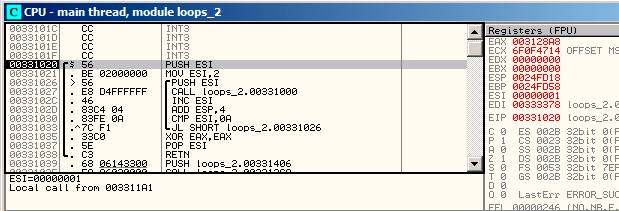
\includegraphics[scale=\FigScale]{patterns/09_loops/simple/olly1.png}
\caption{\olly: \RU{начало \main}\EN{\main begin}}
\label{fig:loops_olly_1}
\end{figure}

\RU{Трассируя}\EN{By tracing} (F8~--- \stepover) \RU{мы видим, как}\EN{we see} \ESI \RU{увеличивается на 1.}
\EN{\glslink{increment}{incrementing}.}
\RU{Например, здесь}\EN{Here, for instance,} $ESI=i=6$:

\begin{figure}[H]
\centering
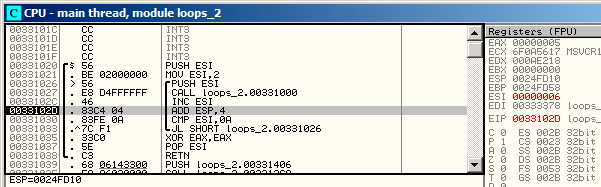
\includegraphics[scale=\FigScale]{patterns/09_loops/simple/olly2.png}
\caption{\olly: \RU{тело цикла только что отработало с}\EN{loop body just executed with} $i=6$}
\label{fig:loops_olly_2}
\end{figure}

9 \RU{это последнее значение цикла}\EN{is the last loop value}.
\RU{Поэтому}\EN{That's why} \JL 
\RU{после \glslink{increment}{инкремента} не срабатывает и функция заканчивается:}
\EN{is not triggering after the \gls{increment}, and the function will finish:}

\begin{figure}[H]
\centering
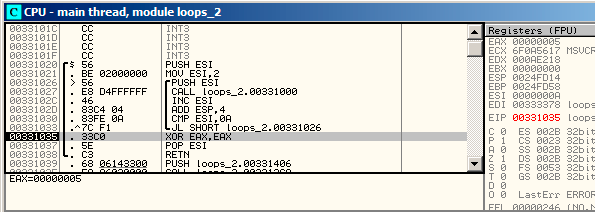
\includegraphics[scale=\FigScale]{patterns/09_loops/simple/olly3.png}
\caption{\olly: $ESI=10$, \RU{конец цикла}\EN{loop end}}
\label{fig:loops_olly_3}
\end{figure}

\subsection{x86: tracer}
\index{tracer}

\RU{Как видно, трассировать вручную цикл в отладчике\EMDASH{}это не очень удобно.}%
\EN{As we might see, it is not very convenient to trace manulally in the debugger.}
\RU{Поэтому попробуем \tracer.}%
\EN{That's a reason we will try \tracer.}

\RU{Открываем скомпилированный пример в \IDA, находим там адрес инструкции \INS{PUSH ESI}
(передающей единственный аргумент в \ttf,)
а это \TT{0x401026} в нашем случае и запускаем \tracer:}
\EN{We open compiled example in \IDA, find the address of the instruction \INS{PUSH ESI}
(passing the sole argument to \ttf,) which is \TT{0x401026} for this case and we run the \tracer:}

\begin{lstlisting}
tracer.exe -l:loops_2.exe bpx=loops_2.exe!0x00401026
\end{lstlisting}

\RU{Опция }\TT{BPX} 
\RU{просто ставит точку останова по адресу и затем tracer будет выдавать состояние регистров.}
\EN{just sets a breakpoint at the address and tracer will then print the state of the registers.}

\RU{В}\EN{In the} \TT{tracer.log} \RU{после запуска я вижу следующее}\EN{This is what we see}:

\lstinputlisting{patterns/09_loops/simple/tracer.log}

\RU{Видно, как значение}\EN{We see how the value of} \ESI \RU{последовательно изменяется от 2 до 9.}
\EN{register changes from 2 to 9.}

\RU{И даже более того, в \tracer можно собирать значения регистров по всем адресам внутри функции.}
\EN{Even more than that, the \tracer can collect register values for all addresses within the function.}
\RU{Там это называется}\EN{This is called} \IT{trace}\EN{ there}.
\RU{Каждая инструкция трассируется, значения самых интересных регистров запоминаются}\EN{Every instruction
gets traced, all interesting register values are recorded}.
\RU{Затем генерируется .idc-скрипт для \IDA, который добавляет комментарии.}
\EN{Then, an \IDA .idc-script is generated, that adds comments.}
\RU{Итак, в}\EN{So, in the} \IDA \RU{я узнал что адрес}\EN{we've learned that the} \main \RU{это}\EN{function address
is} \TT{0x00401020} \RU{и запускаю}\EN{and we run}:

\begin{lstlisting}
tracer.exe -l:loops_2.exe bpf=loops_2.exe!0x00401020,trace:cc
\end{lstlisting}

\TT{BPF} \RU{означает установить точку останова на функции}\EN{stands for set breakpoint on function}.

\RU{Получаю в итоге скрипты}\EN{As a result, we get the} \TT{loops\_2.exe.idc} \AndENRU 
\TT{loops\_2.exe\_clear.idc}\EN{ scripts}.

\clearpage
\RU{Загружаю}\EN{We load} \TT{loops\_2.exe.idc} \RU{в}\EN{into} \IDA \RU{и увижу следующее}\EN{and see}:

\begin{figure}[H]
\centering
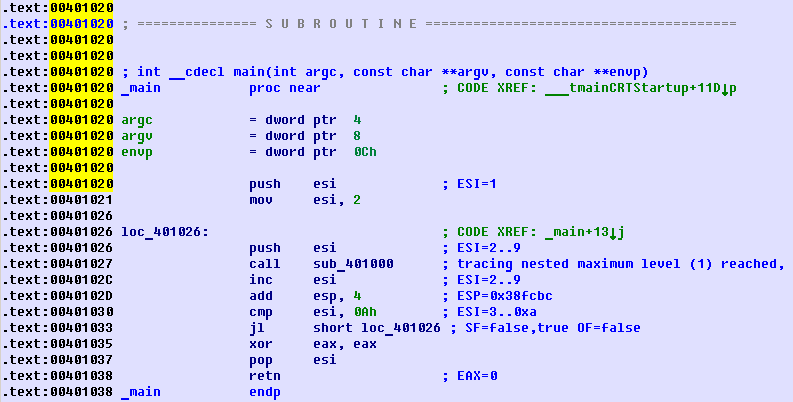
\includegraphics[scale=\FigScale]{patterns/09_loops/simple/IDA_tracer_cc.png}
\caption{\IDA \RU{с загруженным .idc-скриптом}\EN{with .idc-script loaded}}
\label{fig:loops_IDA_tracer}
\end{figure}

\RU{Видно, что}\EN{We see that} \ESI \RU{меняется от 2 до 9 в начале тела цикла, но после 
\glslink{increment}{инкремента} он в пределах [3..0xA]}\EN{can be from 2 to 9 at the start of the loop body,
but from 3 to 0xA (10) after the increment}.
\RU{Видно также, что функция}\EN{We can also see that} \main \RU{заканчивается с 0 в}\EN{is finishing with 0 in} \EAX.

\tracer \RU{также генерирует}\EN{also generates} \TT{loops\_2.exe.txt}, 
\RU{содержащий адреса инструкций, сколько раз была исполнена
каждая и значения регистров}\EN{that contains information about how many times each instruction was executed and
register values}:

\lstinputlisting[caption=loops\_2.exe.txt]{patterns/09_loops/simple/loops_2.exe.txt}
\index{\GrepUsage}
\RU{Так можно использовать grep}\EN{We can use grep here}.

\fi

\ifdefined\IncludeARM
\subsection{ARM}

\subsubsection{\NonOptimizingKeilVI (\ARMMode)}

\lstinputlisting[label=Keil_number_sign]{patterns/09_loops/simple/ARM/Keil_ARM_O0.asm}

\RU{Счетчик итераций $i$ будет храниться в регистре \Reg{4}.}
\EN{Iteration counter $i$ is to be stored in the \Reg{4} register.}

\EN{The}\RU{Инструкция} \TT{\q{MOV R4, \#2}} \RU{просто инициализирует}\EN{instruction just initializes} $i$.

\EN{The}\RU{Инструкции} \TT{\q{MOV R0, R4}} \AndENRU \TT{\q{BL printing\_function}} \RU{составляют тело цикла.}\EN{instructions
compose the body of the loop}, 
\RU{Первая инструкция готовит аргумент для функции, \ttf а вторая вызывает её.}
\EN{the first instruction preparing the argument for \ttf function and the second calling the function.}

\index{ARM!\Instructions!ADD}
\EN{The}\RU{Инструкция} \TT{\q{ADD R4, R4, \#1}} \RU{прибавляет единицу к $i$ при каждой итерации.}
\EN{instruction just adds 1 to the $i$ variable at each iteration.}

\index{ARM!\Instructions!CMP}
\index{ARM!\Instructions!BLT}
\TT{\q{CMP R4, \#0xA}} \RU{сравнивает}\EN{compares} $i$ \RU{с}\EN{with} \TT{0xA} (10). 
\RU{Следующая за ней инструкция \TT{BLT} (\IT{Branch Less Than}) совершит переход, 
если $i$ меньше чем 10.}
\EN{The next instruction \TT{BLT} (\IT{Branch Less Than}) 
jumps if $i$ is less than 10.}

\RU{В противном случае в \Reg{0} запишется 0 (потому что наша функция возвращает 0)
и произойдет выход из функции.}
\EN{Otherwise, 0 is to be written into \Reg{0} (since our function returns 0)
and function execution finishes.}

\subsubsection{\OptimizingKeilVI (\ThumbMode)}

\lstinputlisting{patterns/09_loops/simple/ARM/Keil_thumb_O3.asm}

\RU{Практически всё то же самое.}\EN{Practically the same.}

\subsubsection{\OptimizingXcodeIV (\ThumbTwoMode)}
\label{ARM_unrolled_loops}

\lstinputlisting{patterns/09_loops/simple/ARM/xcode_thumb_O3.asm}

\RU{На самом деле, в моей функции \ttf было такое:}\EN{In fact, this was in my \ttf function:}

\begin{lstlisting}
void printing_function(int i)
{
    printf ("%d\n", i);
};
\end{lstlisting}

\index{Unrolled loop}
\index{Inline code}
\RU{Так что}\EN{So,} LLVM \RU{не только \IT{развернул} цикл}\EN{not just \IT{unrolled} the loop}, 
\RU{но также и представил мою очень простую функцию \ttf как \IT{inline-функцию}}\EN{but also \IT{inlined} my 
very simple function \ttf},
\RU{и вставил её тело вместо цикла 8 раз}\EN{and inserted its body 8 times instead of calling it}. 
\RU{Это возможно, когда функция очень простая (как та что у меня) и когда
она вызывается не очень много раз, как здесь.}
\EN{This is possible when the function is so simple (like mine) and when it is not called too much (like here).}

\subsubsection{ARM64: \Optimizing GCC 4.9.1}

\lstinputlisting[caption=\Optimizing GCC 4.9.1]{patterns/09_loops/simple/ARM/ARM64_GCC491_O3.s.\LANG}

\subsubsection{ARM64: \NonOptimizing GCC 4.9.1}

\lstinputlisting[caption=\NonOptimizing GCC 4.9.1 -fno-inline]{patterns/09_loops/simple/ARM/ARM64_GCC491_O3.s.\LANG}

\fi
\ifdefined\IncludeMIPS
\subsection{MIPS}

\lstinputlisting[caption=\NonOptimizing GCC 4.4.5 (IDA)]{patterns/09_loops/simple/MIPS_O0_IDA.lst.\LANG}

\index{MIPS!\Pseudoinstructions!B}
\RU{Новая для нас инструкция это}\EN{The instruction that's new to us is} \q{B}. 
\RU{Вернее, это псевдоинструкция}\EN{It is actually the pseudoinstruction} (BEQ).

\fi

\subsection{\RU{Ещё кое-что}\EN{One more thing}}

\RU{По генерируемому коду мы видим следующее}\EN{In the generated code we can see}: 
\RU{после инициализации}\EN{after initializing} $i$%
\RU{, тело цикла не исполняется. Исполняется сразу 
проверка условия $i$, а лишь затем исполняется тело цикла.}%
\EN{, the body of the loop is not to be executed,
as the condition for $i$ is checked first, and only after that loop body can be executed.}
\RU{Это правильно.}\EN{And that is correct.} 
\RU{Потому что если условие в самом начале не выполняется, тело цикла исполнять нельзя.}
\EN{Because, if the loop condition is
not met at the beginning, the body of the loop must not be executed.}
\RU{Так может быть, например, в таком случае:}\EN{This is possible in the following case:}

\lstinputlisting{patterns/09_loops/simple/loops_3.c.\LANG}

\RU{Если}\EN{If} \IT{total\_entries\_to\_process} \RU{равно}\EN{is} 0,
\RU{тело цикла не должно исполниться ни разу}\EN{the body of the loo must not be executed at all}.
\RU{Поэтому проверка условия происходит перед тем как исполнить само тело.}
\EN{This is why the condition checked before
the execution.}

\RU{Впрочем, оптимизирующий компилятор может переставить проверку условия и тело цикла местами, если он уверен,
что описанная здесь ситуация невозможна, как в случае с нашим простейшим примером и компиляторами 
Keil, Xcode (LLVM), MSVC и GCC в режиме оптимизации.}
\EN{However, an optimizing compiler may swap the condition check and loop body,
if it sure that the situation described here is
not possible (like in the case of our very simple example and Keil, Xcode (LLVM), MSVC in optimization mode).}

\section{\RU{Функция копирования блоков памяти}\EN{Memory blocks copying routine}}
\label{loop_memcpy}

\RU{Настоящие функции копирования памяти могут копировать по 4 или 8 байт на каждой итерации, использовать \ac{SIMD},
векторизацию, \etc{}.}
\EN{Real-world memory copy routines may copy 4 or 8 bytes at each iteration, use \ac{SIMD}, 
vectorization, \etc{}.}
\RU{Но ради простоты, этот пример настолько прост, насколько это возможно.}
\EN{But for the sake of simplicity, this example is the simplest possible.}

\lstinputlisting{memcpy.c}

\subsection{\RU{Простейшая реализация}\EN{Straight-forward implementation}}

\lstinputlisting[caption=GCC 4.9 x64 \RU{оптимизация по размеру}\EN{optimized for size} (-Os)]{patterns/09_loops/memcpy/memcpy_GCC49_x64_Os.s.\LANG}

\ifdefined\IncludeARM

\lstinputlisting[caption=GCC 4.9 ARM64 \RU{оптимизация по размеру}\EN{optimized for size} (-Os)]{patterns/09_loops/memcpy/memcpy_GCC49_ARM64_Os.s.\LANG}

\lstinputlisting[caption=\OptimizingKeilVI (\ThumbMode)]{patterns/09_loops/memcpy/memcpy_Keil_Thumb_O3.s.\LANG}

\subsection{ARM \RU{в режиме ARM}\EN{in ARM mode}}

\RU{Keil в режиме ARM пользуется условными суффиксами:}
\EN{Keil in ARM mode takes full advantage of conditional suffixes:}

\lstinputlisting[caption=\OptimizingKeilVI (\ARMMode)]{patterns/09_loops/memcpy/memcpy_Keil_ARM_O3.s.\LANG}

\RU{Вот почему здесь только одна инструкция перехода вместо двух.}
\EN{That's why there is only one branch instruction instead of 2.}

\fi

\ifdefined\IncludeMIPS
\subsection{MIPS}

\lstinputlisting[caption=GCC 4.4.5 \RU{оптимизация по размеру}\EN{optimized for size} (-Os) (IDA)]{patterns/09_loops/memcpy/memcpy_MIPS_Os_IDA.lst.\LANG}

\index{MIPS!\Instructions!LBU}
\index{MIPS!\Instructions!SB}
\RU{Здесь две новых для нас инструкций:}
\EN{Here we have two new instructions:} LBU (\q{Load Byte Unsigned}) \AndENRU SB (\q{Store Byte}).
\RU{Так же как и в ARM, все регистры в MIPS имеют длину в 32 бита. Здесь нет частей регистров равных байту,
как в x86.}
\EN{Just like in ARM, all MIPS registers are 32-bit wide, there are no byte-wide parts like in x86.}
\RU{Так что когда нужно работать с байтами, приходится выделять целый 32-битный регистр для этого.}
\EN{So when dealing with single bytes, we have to allocate whole 32-bit registers for them.}
\RU{LBU загружает байт и сбрасывает все остальные биты (\q{Unsigned}).}
\EN{LBU loads a byte and clears all other bits (\q{Unsigned}).}
\index{MIPS!\Instructions!LB}
\RU{И напротив, инструкция LB (\q{Load Byte}) расширяет байт до 32-битного значения учитывая знак.}
\EN{On the other hand, LB (\q{Load Byte}) instruction sign-extends the loaded byte to a 32-bit value.}
\RU{SB просто записывает байт из младших 8 бит регистра в память.}
\EN{SB just writes a byte from lowest 8 bits of register to memory.}

\fi

\ifx\LITE\undefined
\subsection{\RU{Векторизация}\EN{Vectorization}}

\Optimizing GCC \RU{может из этого примера сделать намного больше}\EN{can do much more on this example}: 
\myref{vec_memcpy}.
\fi

\section{\Conclusion{}}

\RU{Примерный скелет цикла от 2 до 9 включительно}\EN{Rough skeleton of loop from 2 to 9 inclusive}:

\lstinputlisting[caption=x86]{patterns/09_loops/skeleton_x86_2_9_optimized.lst.\LANG}

\RU{Операция инкремента может быть представлена как 3 инструкции в неоптимизированном коде:}
\EN{The increment operation may be represented as 3 instructions in non-optimized code:}

\lstinputlisting[caption=x86]{patterns/09_loops/skeleton_x86_2_9.lst.\LANG}

\RU{Если тело цикла короткое, под переменную счетчика можно выделить целый регистр:}
\EN{If the body of the loop is short, a whole register can be dedicated to the counter variable:}

\lstinputlisting[caption=x86]{patterns/09_loops/skeleton_x86_2_9_reg.lst.\LANG}

\RU{Некоторые части цикла могут быть сгенерированы компилятором в другом порядке:}
\EN{Some parts of the loop may be generated by compiler in different order:}

\lstinputlisting[caption=x86]{patterns/09_loops/skeleton_x86_2_9_order.lst.\LANG}

\RU{Обычно условие проверяется \IT{перед} телом цикла, но компилятор может перестроить цикл так, 
что условие проверяется \IT{после} тела цикла.}
\EN{Usually the condition is checked \IT{before} loop body, but the compiler may rearrange it in a way that
the condition is checked \IT{after} loop body.}
\RU{Это происходит тогда, когда компилятор уверен, что условие всегда будет \IT{истинно} на первой итерации,
так что тело цикла исполнится как минимум один раз:}
\EN{This is done when the compiler is sure that the condition is always \IT{true} on the first iteration, 
so the body of the loop is to be executed at least once:}

\lstinputlisting[caption=x86]{patterns/09_loops/skeleton_x86_2_9_reorder.lst.\LANG}

\index{x86!\Instructions!LOOP}
\RU{Используя инструкцию \TT{LOOP}. Это редкость, компиляторы не используют её.
Так что если вы её видите, это верный знак, что этот фрагмент кода написан вручную:}
\EN{Using the \TT{LOOP} instruction. This is rare, compilers are not using it.
When you see it, it's a sign that this piece of code is hand-written:}

\lstinputlisting[caption=x86]{patterns/09_loops/skeleton_x86_loop.lst.\LANG}

\ifdefined\IncludeARM
ARM. 
\RU{В этом примере регистр \Reg{4} выделен для переменной счетчика:}
\EN{The \Reg{4} register is dedicated to counter variable in this example:}

\lstinputlisting[caption=ARM]{patterns/09_loops/skeleton_ARM.lst.\LANG}
\fi

% TODO MIPS

\ifdefined\IncludeExercises
\section{\Exercises}

\subsection{\Exercise \#1}

\index{x86!\Instructions!LOOP}
\RU{Почему инструкция}\EN{Why isn't the} \LOOP \RU{больше не используется современными 
компиляторами}\EN{instruction used by modern compilers anymore}?

\subsection{\Exercise \#2}

\RU{Возьмите пример, рассмотренный в этой секции}\EN{Take a loop example from this section} 
(\myref{loops_src}), 
\RU{скомпилируйте его в вашей любимой}\EN{compile it in your favorite} \ac{OS}
\RU{и компиляторе, и модифицируйте исполняемый файл так, чтобы цикл был в пределах}
\EN{and compiler and modify (patch) the executable file so the loop range will be} [6..20].

\subsection{\Exercise \#3}
\label{exercise_loops_3}

\WhatThisCodeDoes

\begin{lstlisting}[caption=\Optimizing MSVC 2010]
$SG2795	DB	'%d', 0aH, 00H

_main	PROC
	push	esi
	push	edi
	mov	edi, DWORD PTR __imp__printf
	mov	esi, 100
	npad	3 ; align next label
$LL3@main:
	push	esi
	push	OFFSET $SG2795 ; '%d'
	call	edi
	dec	esi
	add	esp, 8
	test	esi, esi
	jg	SHORT $LL3@main
	pop	edi
	xor	eax, eax
	pop	esi
	ret	0
_main	ENDP
\end{lstlisting}

\begin{lstlisting}[caption=\NonOptimizingKeilVI (\ARMMode)]
main PROC
        PUSH     {r4,lr}
        MOV      r4,#0x64
|L0.8|
        MOV      r1,r4
        ADR      r0,|L0.40|
        BL       __2printf
        SUB      r4,r4,#1
        CMP      r4,#0
        MOVLE    r0,#0
        BGT      |L0.8|
        POP      {r4,pc}
        ENDP

|L0.40|
        DCB      "%d\n",0
\end{lstlisting}

\begin{lstlisting}[caption=\NonOptimizingKeilVI (\ThumbMode)]
main PROC
        PUSH     {r4,lr}
        MOVS     r4,#0x64
|L0.4|
        MOVS     r1,r4
        ADR      r0,|L0.24|
        BL       __2printf
        SUBS     r4,r4,#1
        CMP      r4,#0
        BGT      |L0.4|
        MOVS     r0,#0
        POP      {r4,pc}
        ENDP

        DCW      0x0000
|L0.24|
        DCB      "%d\n",0
\end{lstlisting}

\begin{lstlisting}[caption=\Optimizing GCC 4.9 (ARM64)]
main:
	stp	x29, x30, [sp, -32]!
	add	x29, sp, 0
	stp	x19, x20, [sp,16]
	adrp	x20, .LC0
	mov	w19, 100
	add	x20, x20, :lo12:.LC0
.L2:
	mov	w1, w19
	mov	x0, x20
	bl	printf
	subs	w19, w19, #1
	bne	.L2
	ldp	x19, x20, [sp,16]
	ldp	x29, x30, [sp], 32
	ret
.LC0:
	.string	"%d\n"
\end{lstlisting}

\lstinputlisting[caption=\Optimizing GCC 4.4.5 (MIPS) (IDA)]{patterns/09_loops/ex3_MIPS_O3_IDA.lst}

\RU{Ответ}\EN{Answer}: \myref{exercise_solutions_loops_3}.

\subsection{\Exercise \#4}
\label{exercise_loops_4}

\WhatThisCodeDoes

\begin{lstlisting}[caption=\Optimizing MSVC 2010]
$SG2795	DB	'%d', 0aH, 00H

_main	PROC
	push	esi
	push	edi
	mov	edi, DWORD PTR __imp__printf
	mov	esi, 1
	npad	3 ; align next label
$LL3@main:
	push	esi
	push	OFFSET $SG2795 ; '%d'
	call	edi
	add	esi, 3
	add	esp, 8
	cmp	esi, 100
	jl	SHORT $LL3@main
	pop	edi
	xor	eax, eax
	pop	esi
	ret	0
_main	ENDP
\end{lstlisting}

\begin{lstlisting}[caption=\NonOptimizingKeilVI (\ARMMode)]
main PROC
        PUSH     {r4,lr}
        MOV      r4,#1
|L0.8|
        MOV      r1,r4
        ADR      r0,|L0.40|
        BL       __2printf
        ADD      r4,r4,#3
        CMP      r4,#0x64
        MOVGE    r0,#0
        BLT      |L0.8|
        POP      {r4,pc}
        ENDP

|L0.40|
        DCB      "%d\n",0
\end{lstlisting}

\begin{lstlisting}[caption=\NonOptimizingKeilVI (\ThumbMode)]
main PROC
        PUSH     {r4,lr}
        MOVS     r4,#1
|L0.4|
        MOVS     r1,r4
        ADR      r0,|L0.24|
        BL       __2printf
        ADDS     r4,r4,#3
        CMP      r4,#0x64
        BLT      |L0.4|
        MOVS     r0,#0
        POP      {r4,pc}
        ENDP

        DCW      0x0000
|L0.24|
        DCB      "%d\n",0
\end{lstlisting}

\begin{lstlisting}[caption=\Optimizing GCC 4.9 (ARM64)]
main:
	stp	x29, x30, [sp, -32]!
	add	x29, sp, 0
	stp	x19, x20, [sp,16]
	adrp	x20, .LC0
	mov	w19, 1
	add	x20, x20, :lo12:.LC0
.L2:
	mov	w1, w19
	mov	x0, x20
	add	w19, w19, 3
	bl	printf
	cmp	w19, 100
	bne	.L2
	ldp	x19, x20, [sp,16]
	ldp	x29, x30, [sp], 32
	ret
.LC0:
	.string	"%d\n"
\end{lstlisting}

\lstinputlisting[caption=\Optimizing GCC 4.4.5 (MIPS) (IDA)]{patterns/09_loops/ex4_MIPS_O3_IDA.lst}

\RU{Ответ}\EN{Answer}: \myref{exercise_solutions_loops_4}.

\fi

\chapter{\SimpleStringsProcessings}
\index{\CStandardLibrary!strlen()}
\index{\CLanguageElements!while}

% sections
\section{strlen()}
\index{\CStandardLibrary!strlen()}

\RU{Ещё немного о циклах. Часто функция \TT{strlen()}\footnote{подсчет длины строки в Си} 
реализуется при помощи \TT{while()}.}
\EN{Let's talk about loops one more time. Often, the \TT{strlen()} 
function\footnote{counting the characters in a string in the C language} is implemented using a \TT{while()} 
statement.}
\RU{Например, вот как это сделано в стандартных библиотеках MSVC:}
\EN{Here is how it is done in the MSVC standard libraries:}

\lstinputlisting{patterns/10_strings/1_strlen/ex1.c}

% subsections
\subsection{x86}

\subsubsection{\NonOptimizing MSVC}

\RU{Итак, компилируем:}\EN{Let's compile:}

\lstinputlisting{patterns/10_strings/1_strlen/10_1_msvc.asm.\LANG}

\index{x86!\Instructions!MOVSX}
\index{x86!\Instructions!TEST}
\RU{Здесь две новых инструкции: \MOVSX и \TEST.}
\EN{We get two new instructions here: \MOVSX and \TEST.}

\label{MOVSX}
\RU{О первой. \MOVSX предназначена для того, чтобы взять байт из какого-либо места в памяти и положить его, 
в нашем случае, в регистр \EDX. 
Но регистр \EDX~--- 32-битный. \MOVSX означает \IT{MOV with Sign-Extend}. 
Оставшиеся биты с 8-го по 31-й \MOVSX сделает единицей, если исходный байт в памяти имеет знак \IT{минус}, 
или заполнит нулями, если знак \IT{плюс}.}
\EN{The first one---\MOVSX---takes a byte from an address in memory and stores the value in a 32-bit register. 
\MOVSX stands for \IT{MOV with Sign-Extend}. 
\MOVSX sets the rest of the bits, from the 8th to the 31th, 
to 1 if the source byte is \IT{negative} or to 0 if is \IT{positive}.}

\RU{И вот зачем всё это.}\EN{And here is why.}

\RU{По умолчанию в MSVC и GCC тип \Tchar~--- знаковый. Если у нас есть две переменные, одна \Tchar, а другая \Tint 
(\Tint тоже знаковый), и если в первой переменной лежит -2 (что кодируется как \TT{0xFE}) и мы просто 
переложим это в \Tint, 
то там будет \TT{0x000000FE}, а это, с точки зрения \Tint, даже знакового, будет 254, но никак не -2. 
-2 в переменной \Tint кодируется как \TT{0xFFFFFFFE}. Для того чтобы значение \TT{0xFE} из переменной типа 
\Tchar переложить 
в знаковый \Tint с сохранением всего, нужно узнать его знак и затем заполнить остальные биты. 
Это делает \MOVSX.}
\EN{By default, the \Tchar type is signed in MSVC and GCC. If we have two values of which one is \Tchar 
and the other is \Tint, (\Tint is signed too), and if the first value contain -2 (coded as \TT{0xFE}) 
and we just copy this byte into the \Tint container, it makes \TT{0x000000FE}, and this 
from the point of signed \Tint view is 254, but not -2. In signed int, -2 is coded as \TT{0xFFFFFFFE}. 
So if we need to transfer \TT{0xFE} from a variable of \Tchar type to \Tint, 
we need to identify its sign and extend it. That is what \MOVSX does.}

\RU{См. также об этом раздел}
\EN{You can also read about it in} \q{\IT{\SignedNumbersSectionName}}\EN{ section}~(\myref{sec:signednumbers}).

\RU{Хотя конкретно здесь компилятору вряд ли была особая надобность хранить значение \Tchar в регистре \EDX, 
а не его восьмибитной части, скажем \DL. Но получилось, как получилось. Должно быть 
\gls{register allocator} компилятора сработал именно так.}
\EN{It's hard to say if the compiler needs to store a \Tchar variable in \EDX, it could just take a 8-bit register part 
(for example \DL). Apparently, the compiler's \gls{register allocator} works like that.}

\index{ARM!\Instructions!TEST}
\RU{Позже выполняется \TT{TEST EDX, EDX}. 
Об инструкции \TEST читайте в разделе о битовых полях~(\myref{sec:bitfields}).
Конкретно здесь эта инструкция просто проверяет состояние регистра \EDX на 0.}
\EN{Then we see \TT{TEST EDX, EDX}. 
You can read more about the \TEST instruction in the section about bit fields~(\myref{sec:bitfields}).
Here this instruction just checks if the value in \EDX equals to 0.}

\ifdefined\IncludeGCC
\subsubsection{\NonOptimizing GCC}

\RU{Попробуем}\EN{Let's try} GCC 4.4.1:

\lstinputlisting{patterns/10_strings/1_strlen/10_3_gcc.asm}

\label{movzx}
\index{x86!\Instructions!MOVZX}
\RU{Результат очень похож на MSVC, только здесь используется \MOVZX, а не \MOVSX. 
\MOVZX означает \IT{MOV with Zero-Extend}. Эта инструкция перекладывает какое-либо значение 
в регистр и остальные биты выставляет в 0.
Фактически, преимущество этой инструкции только в том, что она позволяет 
заменить две инструкции сразу: \TT{xor eax, eax / mov al, [...]}.}
\EN{The result is almost the same as in MSVC, but here we see \MOVZX instead of \MOVSX. 
\MOVZX stands for \IT{MOV with Zero-Extend}. 
This instruction copies a 8-bit or 16-bit value into a 32-bit register and sets the rest of the bits to 0. 
In fact, this instruction is convenient only because it enable us to replace this instruction pair: 
\TT{xor eax, eax / mov al, [...]}.}

\RU{С другой стороны, нам очевидно, что здесь можно было бы написать вот так: 
\TT{mov al, byte ptr [eax] / test al, al}~--- это тоже самое, хотя старшие биты \EAX будут \q{замусорены}. 
Но будем считать, что это погрешность компилятора~--- 
он не смог сделать код более экономным или более понятным. 
Строго говоря, компилятор вообще не нацелен на то, чтобы генерировать понятный (для человека) код.}
\EN{On the other hand, it is obvious that the compiler could produce this code: 
\TT{mov al, byte ptr [eax] / test al, al}---it is almost the same, however, 
the highest bits of the \EAX register will contain random noise. 
But let's think it is compiler's drawback---it cannot produce more understandable code. 
Strictly speaking, the compiler is not obliged to emit understandable (to humans) code at all.}

\index{x86!\Instructions!SETcc}
\RU{Следующая новая инструкция для нас~--- \SETNZ. В данном случае, если в \AL был не ноль, 
то \TT{test al, al} выставит флаг \ZF в 0, а \SETNZ, если \TT{ZF==0} 
(\IT{NZ} значит \IT{not zero}) выставит 1 в \AL. 
Смысл этой процедуры в том, что 
\IT{если AL не ноль, выполнить переход на} \TT{loc\_80483F0}.
Компилятор выдал немного избыточный код, но не будем забывать, что оптимизация выключена.}
\EN{The next new instruction for us is \SETNZ. 
Here, if \AL doesn't contain zero, \TT{test al, al} 
sets the \ZF flag to 0, but \SETNZ, if \TT{ZF==0} (\IT{NZ} stands for \IT{not zero}) sets \AL to 1.
Speaking in natural language, \IT{if \AL is not zero, let's jump to loc\_80483F0}. 
The compiler emits some redundant code, but let's not forget that the optimizations are turned off.}
\fi

\subsubsection{\Optimizing MSVC}
\label{strlen_MSVC_Ox}

\RU{Теперь скомпилируем всё то же самое в MSVC 2012, но с включенной оптимизацией (\Ox)}
\EN{Now let's compile all this in MSVC 2012, with optimizations turned on (\Ox)}:

\lstinputlisting[caption=\Optimizing MSVC 2012 /Ob0]{patterns/10_strings/1_strlen/10_2.asm.\LANG}

\RU{Здесь всё попроще стало. Но следует отметить, что компилятор обычно может так хорошо использовать регистры 
только на небольших функциях с небольшим количеством локальных переменных.}
\EN{Now it is all simpler.
Needless to say, the compiler could use registers with such efficiency
only in small functions with a few local variables.}

\index{x86!\Instructions!INC}
\index{x86!\Instructions!DEC}
\INC/\DEC\EMDASH\RU{это инструкции \glslink{increment}{инкремента}-\glslink{decrement}{декремента}. Попросту говоря~--- 
увеличить на единицу или уменьшить.}
\EN{are \gls{increment}/\gls{decrement} instructions, in other words: add or substract 1 to/from a variable.}

\ifdefined\IncludeOlly
\input{patterns/10_strings/1_strlen/olly.tex}
\fi

\ifdefined\IncludeGCC
\subsubsection{\Optimizing GCC}

\RU{Попробуем GCC 4.4.1 с включенной оптимизацией (ключ \Othree):}
\EN{Let's check GCC 4.4.1 with optimizations turned on (\Othree key):}

\lstinputlisting{patterns/10_strings/1_strlen/10_3_gcc_O3.asm}

\RU{Здесь GCC не очень отстает от MSVC за исключением наличия \MOVZX.} 
\EN{Here GCC is almost the same as MSVC, except for the presence of \MOVZX.}

\RU{Впрочем, \MOVZX здесь явно можно заменить на}
\EN{However, here \MOVZX could be replaced with} \TT{mov dl, byte ptr [eax]}.

\RU{Но возможно, компилятору GCC просто проще помнить, что у него под переменную типа \Tchar отведен целый 
32-битный регистр \EDX и быть уверенным в том, что старшие биты регистра не будут замусорены.}
\EN{Probably it is simpler for GCC's code generator to \IT{remember} 
the whole 32-bit \EDX register 
is allocated for a \Tchar variable and it then can be sure that the highest bits has no any noise 
at any point.}

\label{strlen_NOT_ADD}
\index{x86!\Instructions!NOT}
\index{x86!\Instructions!XOR}
\RU{Далее мы видим новую для нас инструкцию \NOT. Эта инструкция инвертирует все биты в операнде. 
Можно сказать, что здесь это синонимично инструкции \TT{XOR ECX, 0ffffffffh}. 
\NOT и следующая за ней инструкция \ADD вычисляют разницу указателей и отнимают от результата единицу. 
Только происходит это слегка по-другому. Сначала \ECX, где хранится указатель на \IT{str}, 
инвертируется и от него отнимается единица.}
\EN{After that we also see a new instruction---\NOT. This instruction inverts all bits in the operand. 
You can say that it is a synonym to the \TT{XOR ECX, 0ffffffffh} instruction. 
\NOT and the following \ADD calculate the pointer difference and subtract 1, just in a different way. 
At the start \ECX, where the pointer to \IT{str} is stored, gets inverted and 1 is subtracted from it.}

\RU{См. также раздел:}\EN{See also:} \q{\SignedNumbersSectionName}~(\myref{sec:signednumbers}).

\RU{Иными словами, в конце функции, после цикла, происходит примерно следующее:} 
\EN{In other words, at the end of the function just after loop body, these operations are executed:}

\begin{lstlisting}
ecx=str;
eax=eos;
ecx=(-ecx)-1; 
eax=eax+ecx
return eax
\end{lstlisting}

\dots~\RU{что эквивалентно}\EN{and this is effectively equivalent to}:

\begin{lstlisting}
ecx=str;
eax=eos;
eax=eax-ecx;
eax=eax-1;
return eax
\end{lstlisting}

\RU{Но почему GCC решил, что так будет лучше? Трудно угадать.
Но наверное, оба эти варианта работают примерно одинаково в плане эффективности и скорости.}
\EN{Why did GCC decide it would be better? Hard to guess. 
But perhaps the both variants are equivalent in efficiency.}
\fi

\ifdefined\IncludeARM
\subsection{ARM}

% subsubsections
\input{patterns/10_strings/1_strlen/ARM/ARM32}
\input{patterns/10_strings/1_strlen/ARM/ARM64}

\fi
\ifdefined\IncludeMIPS
\subsection{MIPS}

\lstinputlisting[caption=\Optimizing GCC 4.4.5 (IDA)]{patterns/10_strings/1_strlen/MIPS_O3_IDA.lst.\LANG}

\index{MIPS!\Instructions!NOR}
\index{MIPS!\Pseudoinstructions!NOT}
\RU{В MIPS нет инструкции \NOT, но есть \NOR~--- операция \TT{OR~+~NOT}.}
\EN{MIPS lacks a \NOT instruction, but has \NOR which is \TT{OR~+~NOT} operation.}
\RU{Эта операция широко применяется в цифровой электронике\footnote{\NOR называют \q{универсальным элементом}.
Например, космический компьютер Apollo Guidance Computer использовавшийся в программе \q{Аполлон} был
построен исключительно на 5600 элементах \NOR: \cite{Eickhoff}.}, но не очень популярна в программировании.}
\EN{This operation is widely used in digital electronics\footnote{NOR is called \q{universal gate}.
For example, the Apollo Guidance Computer used in the Apollo program, 
was built by only using 5600 NOR gates: \cite{Eickhoff}.}, but isn't very popular in computer programming.}
\RU{Так что операция \NOT реализована здесь как}\EN{So, the NOT operation is implemented here as} 
\TT{NOR~DST,~\$ZERO,~SRC}.

\RU{Из фундаментальных знаний \myref{sec:signednumbers}, мы можем знать, что побитовое инвертирование знакового
числа это то же что и смена его знака с вычитанием 1 из результата.}
\EN{From fundamentals \myref{sec:signednumbers} we know that bitwise inverting a signed number is the same 
as changing its sign and subtracting 1 from the result.}
\RU{Так что \NOT берет значение $str$ и трансформирует его в $-str-1$.}
\EN{So what \NOT does here is to take the value of $str$ and transform it into $-str-1$.}
\RU{Следующая операция сложения готовит результат}\EN{The addition operation that follows prepares result}.

\fi

\ifdefined\IncludeExercises
\section{\Exercises}

\subsection{\Exercise \#1}
\label{exercise_strlen_1}

\WhatThisCodeDoes\

\begin{lstlisting}[caption=\Optimizing MSVC 2010]
_s$ = 8			
_f	PROC
	mov	edx, DWORD PTR _s$[esp-4]
	mov	cl, BYTE PTR [edx]
	xor	eax, eax
	test	cl, cl
	je	SHORT $LN2@f
	npad	4 ; align next label
$LL4@f:
	cmp	cl, 32	
	jne	SHORT $LN3@f
	inc	eax
$LN3@f:
	mov	cl, BYTE PTR [edx+1]
	inc	edx
	test	cl, cl
	jne	SHORT $LL4@f
$LN2@f:
	ret	0
_f	ENDP
\end{lstlisting}

\begin{lstlisting}[caption=GCC 4.8.1 -O3]
f:
.LFB24:
	push	ebx
	mov	ecx, DWORD PTR [esp+8]
	xor	eax, eax
	movzx	edx, BYTE PTR [ecx]
	test	dl, dl
	je	.L2
.L3:
	cmp	dl, 32
	lea	ebx, [eax+1]
	cmove	eax, ebx
	add	ecx, 1
	movzx	edx, BYTE PTR [ecx]
	test	dl, dl
	jne	.L3
.L2:
	pop	ebx
	ret
\end{lstlisting}

\begin{lstlisting}[caption=\OptimizingKeilVI (\ARMMode)]
f PROC
        MOV      r1,#0
|L0.4|
        LDRB     r2,[r0,#0]
        CMP      r2,#0
        MOVEQ    r0,r1
        BXEQ     lr
        CMP      r2,#0x20
        ADDEQ    r1,r1,#1
        ADD      r0,r0,#1
        B        |L0.4|
        ENDP
\end{lstlisting}

\begin{lstlisting}[caption=\OptimizingKeilVI (\ThumbMode)]
f PROC
        MOVS     r1,#0
        B        |L0.12|
|L0.4|
        CMP      r2,#0x20
        BNE      |L0.10|
        ADDS     r1,r1,#1
|L0.10|
        ADDS     r0,r0,#1
|L0.12|
        LDRB     r2,[r0,#0]
        CMP      r2,#0
        BNE      |L0.4|
        MOVS     r0,r1
        BX       lr
        ENDP
\end{lstlisting}

\begin{lstlisting}[caption=\Optimizing GCC 4.9 (ARM64)]
f:
	ldrb	w1, [x0]
	cbz	w1, .L4
	mov	w2, 0
.L3:
	cmp	w1, 32
	ldrb	w1, [x0,1]!
	csinc	w2, w2, w2, ne
	cbnz	w1, .L3
.L2:
	mov	w0, w2
	ret
.L4:
	mov	w2, w1
	b	.L2
\end{lstlisting}

\lstinputlisting[caption=\Optimizing GCC 4.4.5 (MIPS) (IDA)]{patterns/10_strings/ex_MIPS_O3_IDA.lst}

\Answer\: \myref{exercise_solutions_strlen_1}.

\fi

\chapter{\ArithOptimizations}

\RU{В целях оптимизации одна инструкция может быть заменена другой, или даже группой инструкций.}
\EN{In the pursuit of optimization, one instruction may be replaced by another, 
or even with a group of instructions.} \RU{Например}\EN{For example}, \ADD \AndENRU \SUB \RU{могут заменять друг друга}\EN{can replace each other}:
\LineENRU 18 \InENRU \lstref{neg_array_c}.

\ifx\LITE\undefined
\RU{Более того, не всегда замена тривиальна. Инструкция \LEA, несмотря на оригинальное назначение, нередко применяется для простых арифметических действий:}
\EN{For example, the \LEA instruction is often used for simple arithmetic calculations:}  \myref{sec:LEA}.

\fi

% sections
\section{\RU{Умножение}\EN{Multiplication}}

\subsection{\RU{Умножение при помощи сложения}\EN{Multiplication using addition}}

\RU{Вот простой пример}\EN{Here is a simple example}:

\begin{lstlisting}[caption=\Optimizing MSVC 2010]
unsigned int f(unsigned int a)
{
	return a*8;
};
\end{lstlisting}

\RU{Умножение на 8 заменяется на три инструкции сложения, делающих то же самое.}
\EN{Multiplication by 8 is replaced by 3 addition instructions, which do the same.}
\RU{Должно быть, оптимизатор в MSVC решил, что этот код может быть быстрее.}
\EN{Apparently, MSVC's optimizer decided that this code can be faster.}

\begin{lstlisting}
_TEXT	SEGMENT
_a$ = 8							; size = 4
_f	PROC
; File c:\polygon\c\2.c
	mov	eax, DWORD PTR _a$[esp-4]
	add	eax, eax
	add	eax, eax
	add	eax, eax
	ret	0
_f	ENDP
_TEXT	ENDS
END
\end{lstlisting}

\subsection{\RU{Умножение при помощи сдвигов}\EN{Multiplication using shifting}}
\label{subsec:mult_using_shifts}

\RU{Ещё очень часто умножения и деления на числа вида $2^{n}$ заменяются на инструкции сдвигов.}
\EN{Multiplication and division instructions by a numbers that's a power of 2 are often replaced
by shift instructions.}

\begin{lstlisting}
unsigned int f(unsigned int a)
{
	return a*4;
};
\end{lstlisting}

\begin{lstlisting}[caption=\NonOptimizing MSVC 2010]
_a$ = 8		; size = 4
_f	PROC
	push	ebp
	mov	ebp, esp
	mov	eax, DWORD PTR _a$[ebp]
	shl	eax, 2
	pop	ebp
	ret	0
_f	ENDP
\end{lstlisting}

\RU{Умножить на 4 это просто сдвинуть число на 2 бита влево, 
вставив 2 нулевых бита справа (как два самых младших бита). 
Это как умножить 3 на 100~--- нужно просто дописать два нуля справа.}
\EN{Multiplication by 4 is just shifting the number to the left by 2 bits
and inserting 2 zero bits at the right (as the last two bits).
It is just like multiplying 3 by 100~---we need to just add two zeroes at the right.}

\RU{Вот как работает инструкция сдвига влево}\EN{That's how the shift left instruction works}:

\index{x86!\Instructions!SHL}
\begin{center}
	\begin{tikzpicture}[scale=0.7, every node/.style={scale=0.7}]
	\edef\bitsize{1cm}
	\tikzstyle{byte}=[draw,minimum size=\bitsize]	
	\tikzstyle{every path}=[thick]

	\node [draw,rectangle,minimum size=\bitsize] (a1) {7};
	\node [draw,rectangle,minimum size=\bitsize] (a2) [right of=a1] {6};
	\node [draw,rectangle,minimum size=\bitsize] (a3) [right of=a2] {5};
	\node [draw,rectangle,minimum size=\bitsize] (a4) [right of=a3] {4};
	\node [draw,rectangle,minimum size=\bitsize] (a5) [right of=a4] {3};
	\node [draw,rectangle,minimum size=\bitsize] (a6) [right of=a5] {2};
	\node [draw,rectangle,minimum size=\bitsize] (a7) [right of=a6] {1};
	\node [draw,rectangle,minimum size=\bitsize] (a8) [right of=a7] {0};

	\node (empty) [below of=a1] {};

	\node [draw,rectangle,minimum size=\bitsize] (b1) [below of=empty] {7};
	\node [draw,rectangle,minimum size=\bitsize] (b2) [right of=b1] {6};
	\node [draw,rectangle,minimum size=\bitsize] (b3) [right of=b2] {5};
	\node [draw,rectangle,minimum size=\bitsize] (b4) [right of=b3] {4};
	\node [draw,rectangle,minimum size=\bitsize] (b5) [right of=b4] {3};
	\node [draw,rectangle,minimum size=\bitsize] (b6) [right of=b5] {2};
	\node [draw,rectangle,minimum size=\bitsize] (b7) [right of=b6] {1};
	\node [draw,rectangle,minimum size=\bitsize] (b8) [right of=b7] {0};
	
	\node [shape=rectangle,draw,minimum size=\bitsize] (d) [left=of b1] {CF};
	\node [shape=rectangle,draw,minimum size=\bitsize] (c) [right=of b8] {0};
	
	\draw [->] (c.west) -- (b8.east);

	\draw [->] (a2.south) -- (b1.north);
	\draw [->] (a3.south) -- (b2.north);
	\draw [->] (a4.south) -- (b3.north);
	\draw [->] (a5.south) -- (b4.north);
	\draw [->] (a6.south) -- (b5.north);
	\draw [->] (a7.south) -- (b6.north);
	\draw [->] (a8.south) -- (b7.north);
	
	\draw [->] (a1.south) -- (d.north);

	\end{tikzpicture}
\end{center}


\RU{Добавленные биты справа~--- всегда нули}\EN{The added bits at right are always zeroes}.

\ifdefined\IncludeARM
\RU{Умножение на 4 в}\EN{Multiplication by 4 in} ARM:

\begin{lstlisting}[caption=\NonOptimizingKeilVI (\ARMMode)]
f PROC
        LSL      r0,r0,#2
        BX       lr
        ENDP
\end{lstlisting}
\fi

\ifdefined\IncludeMIPS
\RU{Умножение на 4 в}\EN{Multiplication by 4 in} MIPS:

\lstinputlisting[caption=\Optimizing GCC 4.4.5 (IDA)]{patterns/11_arith_optimizations/MIPS_SLL.lst}

\index{MIPS!\Instructions!SLL}
SLL \RU{это}\EN{is} \q{Shift Left Logical}.
\fi

\subsection{\RU{Умножение при помощи сдвигов, сложений и вычитаний}
\EN{Multiplication using shifting, subtracting, and adding}}
\label{multiplication_using_shifts_adds_subs}

\RU{Можно избавиться от операции умножения, если вы умножаете на числа вроде 7 или 17,
и использовать сдвиги.}
\EN{It's still possible to get rid of the multiplication operation when you multiply by numbers like
7 or 17 again by using shifting.}
\RU{Здесь используется относительно простая математика}\EN{The mathematics used here is relatively easy}.

\subsubsection{32-\EN{bit}\RU{бита}}

\lstinputlisting{patterns/11_arith_optimizations/mult_shifts.c}

\myparagraph{x86}

\lstinputlisting[caption=\Optimizing MSVC 2012]{patterns/11_arith_optimizations/mult_shifts_MSVC_2012_Ox.asm}

\ifdefined\IncludeARM
\myparagraph{ARM}

\RU{Keil, генерируя код для режима ARM, использует модификаторы инструкции, в которых можно задавать
сдвиг для второго операнда:}
\EN{Keil for ARM mode takes advantage of the second operand's shift modifiers:}

\lstinputlisting[caption=\OptimizingKeilVI (\ARMMode)]{patterns/11_arith_optimizations/mult_shifts_Keil_ARM_O3.s}

\RU{Но таких модификаторов в режиме Thumb нет.}
\EN{But there are no such modifiers in Thumb mode.}
\RU{И он также не смог оптимизировать функцию \TT{f2()}}\EN{It also can't optimize \TT{f2()}}:

\lstinputlisting[caption=\OptimizingKeilVI (\ThumbMode)]{patterns/11_arith_optimizations/mult_shifts_Keil_thumb_O3.s}
\fi

\ifdefined\IncludeMIPS
\myparagraph{MIPS}

\lstinputlisting[caption=\Optimizing GCC 4.4.5 (IDA)]{patterns/11_arith_optimizations/mult_shifts_MIPS_O3_IDA.lst}
\fi

\subsubsection{64-\EN{bit}\RU{бита}}

\lstinputlisting{patterns/11_arith_optimizations/mult_shifts_64.c}

\myparagraph{x64}

\lstinputlisting[caption=\Optimizing MSVC 2012]{patterns/11_arith_optimizations/mult_shifts_64_GCC49_x64_O3.s}

\ifdefined\IncludeARM
\myparagraph{ARM64}

\ifdefined\IncludeGCC
\RU{GCC 4.9 для ARM64 также очень лаконичен благодаря модификаторам сдвига:}
\EN{GCC 4.9 for ARM64 is also terse, thanks to the shift modifiers:}

\lstinputlisting[caption=\Optimizing GCC (Linaro) 4.9 ARM64]{patterns/11_arith_optimizations/mult_shifts_64_GCC49_ARM64.s}
\fi
\fi

\section{\RU{Деление}\EN{Division}}

\subsection{\RU{Деление используя сдвиги}\EN{Division using shifts}}
\label{division_by_shifting}

\RU{Например, возьмем деление на 4}\EN{Example of division by 4}:

\begin{lstlisting}
unsigned int f(unsigned int a)
{
	return a/4;
};
\end{lstlisting}

\RU{Имеем в итоге}\EN{We get} (MSVC 2010):

\begin{lstlisting}[caption=MSVC 2010]
_a$ = 8							; size = 4
_f	PROC
	mov	eax, DWORD PTR _a$[esp-4]
	shr	eax, 2
	ret	0
_f	ENDP
\end{lstlisting}

\label{SHR}
\index{x86!\Instructions!SHR}
\RU{Инструкция \SHR (\IT{SHift Right}) в данном примере сдвигает число на 2 бита вправо. 
При этом освободившиеся два бита слева (т.е. самые 
старшие разряды) выставляются в нули. А самые младшие 2 бита выкидываются. 
Фактически, эти два выкинутых бита~--- остаток от деления.}
\EN{The \SHR (\IT{SHift Right}) instruction in this example is shifting a number by 2 bits to the right.
The two freed bits at left (e.g., two most significant bits) are set to zero.
The two least significant bits are dropped.
In fact, these two dropped bits are the division operation remainder.}

\index{x86!\Instructions!SHR}
\RU{Инструкция \SHR работает так же как и \SHL, только в другую сторону.}
\EN{The \SHR instruction works just like \SHL, but in the other direction.}

\begin{center}
	\begin{tikzpicture}[scale=0.7, every node/.style={scale=0.7}]
	\edef\bitsize{1cm}
	\tikzstyle{byte}=[draw,minimum size=\bitsize]	
	\tikzstyle{every path}=[thick]

	\node [draw,rectangle,minimum size=\bitsize] (a1) {7};
	\node [draw,rectangle,minimum size=\bitsize] (a2) [right of=a1] {6};
	\node [draw,rectangle,minimum size=\bitsize] (a3) [right of=a2] {5};
	\node [draw,rectangle,minimum size=\bitsize] (a4) [right of=a3] {4};
	\node [draw,rectangle,minimum size=\bitsize] (a5) [right of=a4] {3};
	\node [draw,rectangle,minimum size=\bitsize] (a6) [right of=a5] {2};
	\node [draw,rectangle,minimum size=\bitsize] (a7) [right of=a6] {1};
	\node [draw,rectangle,minimum size=\bitsize] (a8) [right of=a7] {0};

	\node (empty) [below of=a1] {};

	\node [draw,rectangle,minimum size=\bitsize] (b1) [below of=empty] {7};
	\node [draw,rectangle,minimum size=\bitsize] (b2) [right of=b1] {6};
	\node [draw,rectangle,minimum size=\bitsize] (b3) [right of=b2] {5};
	\node [draw,rectangle,minimum size=\bitsize] (b4) [right of=b3] {4};
	\node [draw,rectangle,minimum size=\bitsize] (b5) [right of=b4] {3};
	\node [draw,rectangle,minimum size=\bitsize] (b6) [right of=b5] {2};
	\node [draw,rectangle,minimum size=\bitsize] (b7) [right of=b6] {1};
	\node [draw,rectangle,minimum size=\bitsize] (b8) [right of=b7] {0};
	
	\node [shape=rectangle,draw,minimum size=\bitsize] (c) [left=of b1] {0};
	\node [shape=rectangle,draw,minimum size=\bitsize] (d) [right=of b8] {CF};
	
	\draw [->] (c.east) -- (b1.west);

	\draw [->] (a1.south) -- (b2.north);
	\draw [->] (a2.south) -- (b3.north);
	\draw [->] (a3.south) -- (b4.north);
	\draw [->] (a4.south) -- (b5.north);
	\draw [->] (a5.south) -- (b6.north);
	\draw [->] (a6.south) -- (b7.north);
	\draw [->] (a7.south) -- (b8.north);
	
	\draw [->] (a8.south) -- (d.north);

	\end{tikzpicture}
\end{center}



\RU{Для того, чтобы это проще понять, представьте себе десятичную систему счисления и число 23. 
23 можно разделить на 10 просто откинув последний разряд (3~--- это остаток от деления). 
После этой операции останется 2 как \glslink{quotient}{частное}.}
\EN{It is easy to understand if you imagine the number 23 in the decimal numeral system.
23 can be easily divided by 10 just by dropping last digit (3---division remainder). 
2 is left after the operation as a \gls{quotient}.}
\PTBRph{}\ESph{}\PLph{}\\
\\
\RU{Так что остаток выбрасывается, но это нормально, мы все-таки работаем с целочисленными
значениями, а не с \glslink{real number}{вещественными}!}
\EN{So the remainder is dropped, but that's OK, we work on integer values anyway, 
these are not a \glslink{real number}{real numbers}!}\\
\\
\ifdefined\IncludeARM
\RU{Деление на 4 в}\EN{Division by 4 in} ARM:

\begin{lstlisting}[caption=\NonOptimizingKeilVI (\ARMMode)]
f PROC
        LSR      r0,r0,#2
        BX       lr
        ENDP
\end{lstlisting}
\fi

\ifdefined\IncludeMIPS
\RU{Деление на 4 в}\EN{Division by 4 in} MIPS:

\begin{lstlisting}[caption=\Optimizing GCC 4.4.5 (IDA)]
                 jr      $ra
                 srl     $v0, $a0, 2 ; branch delay slot
\end{lstlisting}

\index{MIPS!\Instructions!SRL}
\RU{Инструкция SRL это}\EN{The SRL instruction is} \q{Shift Right Logical}.
\fi

\ifdefined\IncludeExercises
\section{\Exercises}

% 1

\subsection{\Exercise \#2}
\label{exercise_arith_optimizations_2}

\WhatThisCodeDoes\

\begin{lstlisting}[caption=\Optimizing MSVC 2010]
_a$ = 8
_f	PROC
	mov	ecx, DWORD PTR _a$[esp-4]
	lea	eax, DWORD PTR [ecx*8]
	sub	eax, ecx
	ret	0
_f	ENDP
\end{lstlisting}

\begin{lstlisting}[caption=\NonOptimizingKeilVI (\ARMMode)]
f PROC
        RSB      r0,r0,r0,LSL #3
        BX       lr
        ENDP
\end{lstlisting}

\begin{lstlisting}[caption=\NonOptimizingKeilVI (\ThumbMode)]
f PROC
        LSLS     r1,r0,#3
        SUBS     r0,r1,r0
        BX       lr
        ENDP
\end{lstlisting}

\begin{lstlisting}[caption=\Optimizing GCC 4.9 (ARM64)]
f:
	lsl	w1, w0, 3
	sub	w0, w1, w0
	ret
\end{lstlisting}

\begin{lstlisting}[caption=\Optimizing GCC 4.4.5 (MIPS) (IDA)]
f:
                sll     $v0, $a0, 3
                jr      $ra
                subu    $v0, $a0
\end{lstlisting}

\Answer\: \myref{exercise_solutions_arith_optimizations_2}.

\fi

\ifx\LITE\undefined
\chapter{\FPUChapterName}
\label{sec:FPU}

\newcommand{\FNURLSTACK}{\footnote{\href{http://go.yurichev.com/17123}{wikipedia.org/wiki/Stack\_machine}}}
\newcommand{\FNURLFORTH}{\footnote{\href{http://go.yurichev.com/17124}{wikipedia.org/wiki/Forth\_(programming\_language)}}}
\newcommand{\FNURLIEEE}{\footnote{\href{http://go.yurichev.com/17125}{wikipedia.org/wiki/IEEE\_floating\_point}}}
\newcommand{\FNURLSP}{\footnote{\href{http://go.yurichev.com/17126}{wikipedia.org/wiki/Single-precision\_floating-point\_format}}}
\newcommand{\FNURLDP}{\footnote{\href{http://go.yurichev.com/17127}{wikipedia.org/wiki/Double-precision\_floating-point\_format}}}
\newcommand{\FNURLEP}{\footnote{\href{http://go.yurichev.com/17128}{wikipedia.org/wiki/Extended\_precision}}}

\RU{\ac{FPU}\EMDASH блок в процессоре работающий с числами с плавающей запятой.}
\EN{The \ac{FPU} is a device within the main \ac{CPU}, specially designed to deal with floating point numbers.}
\RU{Раньше он назывался \q{сопроцессором} и он стоит немного в стороне от \ac{CPU}.}
\EN{It was called \q{coprocessor} in the past and it stays somewhat aside of the main \ac{CPU}.}

\section{IEEE 754}

\RU{Число с плавающей точкой в формате IEEE 754 состоит из \IT{знака}, \IT{мантиссы}\footnote{\IT{significand} или \IT{fraction} 
в англоязычной литературе} и \IT{экспоненты}.}
\EN{A number in the IEEE 754 format consists of a \IT{sign}, a \IT{significand} (also called \IT{fraction}) and an \IT{exponent}.}

\section{x86}

\RU{Перед изучением \ac{FPU} в x86 полезно ознакомиться с тем как работают стековые машины\FNURLSTACK 
или ознакомиться с основами языка Forth\FNURLFORTH.}
\EN{It is worth looking into stack machines\FNURLSTACK or learning the basics of the Forth language\FNURLFORTH,
before studying the \ac{FPU} in x86.}

\index{Intel!80486}
\index{Intel!FPU}
\RU{Интересен факт, что в свое время (до 80486) сопроцессор был отдельным чипом на материнской плате, 
и вследствие его высокой цены, он не всегда присутствовал. Его можно было докупить и установить отдельно}%
\EN{It is interesting to know that in the past (before the 80486 CPU) the coprocessor was a separate chip 
and it was not always pre-installed on the motherboard. It was possible to buy it separately and install it}%
\footnote{\RU{Например, Джон Кармак использовал в своей игре Doom числа с фиксированной запятой 
(\href{http://go.yurichev.com/17357}{ru.wikipedia.org/wiki/Число\_с\_фиксированной\_запятой}), хранящиеся
в обычных 32-битных \ac{GPR} (16 бит на целую часть и 16 на дробную),
чтобы Doom работал на 32-битных компьютерах без FPU, т.е. 80386 и 80486 SX.}
\EN{For example, John Carmack used fixed-point arithmetic 
(\href{http://go.yurichev.com/17356}{wikipedia.org/wiki/Fixed-point\_arithmetic}) values in his Doom video game, stored in 
32-bit \ac{GPR} registers (16 bit for integral part and another 16 bit for fractional part), so Doom
could work on 32-bit computers without FPU, i.e., 80386 and 80486 SX.}}.
\RU{Начиная с 80486 DX в состав процессора всегда входит FPU.}
\EN{Starting with the 80486 DX CPU, the \ac{FPU} is integrated in the \ac{CPU}.}

\index{x86!\Instructions!FWAIT}
\RU{Этот факт может напоминать такой рудимент как наличие инструкции \TT{FWAIT}, 
которая заставляет
\ac{CPU} ожидать, пока \ac{FPU} закончит работу}\EN{The \TT{FWAIT} instruction reminds us of that fact---it
switches the \ac{CPU} to a waiting state, so it can wait until the \ac{FPU} is done with its work}.
\RU{Другой рудимент это тот факт, что опкоды \ac{FPU}-инструкций начинаются с т.н. \q{escape}-опкодов 
(\TT{D8..DF}) как опкоды, передающиеся в отдельный сопроцессор.}
\EN{Another rudiment is the fact that the \ac{FPU} instruction 
opcodes start with the so called \q{escape}-opcodes (\TT{D8..DF}), i.e., 
opcodes passed to a separate coprocessor.}

\index{IEEE 754}
\label{FPU_is_stack}
\RU{FPU имеет стек из восьми 80-битных регистров:}
\EN{The FPU has a stack capable to holding 8 80-bit registers, and each register can hold a number 
in the IEEE 754\FNURLIEEE format.}
\RU{\ST{0}..\ST{7}. Для краткости, IDA и \olly отображают \ST{0} как \TT{ST},
что в некоторых учебниках и документациях означает \q{Stack Top} (\q{вершина стека}).}
\RU{Каждый регистр может содержать число в формате IEEE 754\FNURLIEEE.}
\EN{They are \ST{0}..\ST{7}. For brevity, IDA and \olly show \ST{0} as \TT{ST}, 
which is represented in some textbooks and manuals as \q{Stack Top}.}

\section{ARM, MIPS, x86/x64 SIMD}

\RU{В ARM и MIPS FPU это не стек, а просто набор регистров.}
\EN{In ARM and MIPS the FPU is not a stack, but a set of registers.}
\RU{Такая же идеология применяется в расширениях SIMD в процессорах x86/x64.}
\EN{The same ideology is used in the SIMD extensions of x86/x64 CPUs.}

\section{\CCpp}

\index{float}
\index{double}
\RU{В стандартных \CCpp имеются два типа для работы с числами с плавающей запятой: 
\Tfloat (\IT{число одинарной точности}\FNURLSP, 32 бита)
\footnote{Формат представления чисел с плавающей точкой одинарной точности затрагивается в разделе 
\IT{\WorkingWithFloatAsWithStructSubSubSectionName}~(\myref{sec:floatasstruct}).}
и \Tdouble (\IT{число двойной точности}\FNURLDP, 64 бита).}
\EN{The standard \CCpp languages offer at least two floating number types, \Tfloat (\IT{single-precision}\FNURLSP, 32 bits)
\footnote{the single precision floating point number format is also addressed in 
the \IT{\WorkingWithFloatAsWithStructSubSubSectionName}~(\myref{sec:floatasstruct}) section}
and \Tdouble (\IT{double-precision}\FNURLDP, 64 bits).}

\index{long double}
\RU{GCC также поддерживает тип \IT{long double} (\IT{extended precision}\FNURLEP, 80 бит), но MSVC~--- нет.}
\EN{GCC also supports the \IT{long double} type (\IT{extended precision}\FNURLEP, 80 bit), which MSVC doesn't.}

\RU{Несмотря на то, что \Tfloat занимает столько же места, сколько и \Tint на 32-битной архитектуре, 
представление чисел, разумеется, совершенно другое.}
\EN{The \Tfloat type requires the same number of bits as the \Tint type in 32-bit environments, 
but the number representation is completely different.}

\section{\RU{Простой пример}\EN{Simple example}}

\RU{Рассмотрим простой пример}\EN{Let's consider this simple example}:

\lstinputlisting{patterns/12_FPU/1_simple/simple.c}

\subsection{x86}

% subsubsections
\input{patterns/12_FPU/1_simple/MSVC}
\input{patterns/12_FPU/1_simple/GCC}

\ifdefined\IncludeARM
\subsection{ARM: \OptimizingXcodeIV (\ARMMode)}

\RU{Пока в ARM не было стандартного набора инструкций для работы с числами с плавающей точкой}%
\EN{Until ARM got standardized floating point support}, \RU{разные производители процессоров
могли добавлять свои расширения для работы с ними}\EN{several processor manufacturers added their own 
instructions extensions}.
\RU{Позже был принят стандарт}\EN{Then, } VFP (\IT{Vector Floating Point})\EN{ was standardized}.

\RU{Важное отличие от x86 в том, что там вы работаете с FPU-стеком, а здесь стека нет, 
вы работаете просто с регистрами.}
\EN{One important difference from x86 is that in ARM, there
is no stack, you work just with registers.}

\lstinputlisting[label=ARM_leaf_example10,caption=\OptimizingXcodeIV (\ARMMode)]{patterns/12_FPU/1_simple/ARM/Xcode_ARM_O3.asm.\LANG}

\index{ARM!D-\registers{}}
\index{ARM!S-\registers{}}
\RU{Итак, здесь мы видим использование новых регистров с префиксом D.}
\EN{So, we see here new some registers used, with D prefix.}
\RU{Это 64-битные регистры. Их 32 и их можно
использовать для чисел с плавающей точкой двойной точности (double) и для 
SIMD (в ARM это называется NEON).}
\EN{These are 64-bit registers, there are 32 of them, and they can be used both for floating-point numbers 
(double) but also for SIMD (it is called NEON here in ARM).}
\RU{Имеются также 32 32-битных S-регистра. Они применяются для работы с числами 
с плавающей точкой одинарной точности (float).}
\EN{There are also 32 32-bit S-registers, intended to be used for single precision 
floating pointer numbers (float).}
\RU{Запомнить легко: D-регистры предназначены для чисел double-точности, 
а S-регистры~--- для чисел single-точности.}
\EN{It is easy to remember: D-registers are for double precision numbers, while
S-registers---for single precision numbers.}
\RU{Больше об этом}\EN{More about it}: \myref{ARM_VFP_registers}.

\RU{Обе константы (3,14 и 4,1)}\EN{Both constants (3.14 and 4.1)} \RU{хранятся в памяти в формате IEEE 754.}
\EN{are stored in memory in IEEE 754 format.}

\index{ARM!\Instructions!VLDR}
\index{ARM!\Instructions!VMOV}
\RU{Инструкции }\TT{VLDR} \AndENRU \TT{VMOV}%
\RU{, как можно догадаться, это аналоги обычных \TT{LDR} и \MOV, но они работают с D-регистрами.}
\EN{, as it can be easily deduced, are analogous to the \TT{LDR} and \MOV instructions,
but they work with D-registers.}
\RU{Важно отметить, что эти инструкции, как и D-регистры, предназначены не только для работы 
с числами с плавающей точкой, но пригодны также и для работы с SIMD (NEON), и позже это также будет видно.}
\EN{It has to be noted that these instructions, just like the D-registers, are intended not only for
floating point numbers, 
but can be also used for SIMD (NEON) operations and this will also be shown soon.}

\RU{Аргументы передаются в функцию обычным путем через R-регистры, однако 
каждое число, имеющее двойную точность, занимает 64 бита, так что для передачи каждого нужны два R-регистра.}
\EN{The arguments are passed to the function in a common way, via the R-registers, however
each number that has double precision has a size of 64 bits, so two R-registers are needed to pass each one.}

\TT{VMOV D17, R0, R1} \RU{в самом начале составляет два 32-битных значения из \Reg{0} и \Reg{1} 
в одно 64-битное и сохраняет в}
\EN{at the start, composes two 32-bit values from \Reg{0} and \Reg{1} into one 64-bit value
and saves it to} \TT{D17}.

\TT{VMOV R0, R1, D16} \RU{в конце это обратная процедура}\EN{is the inverse operation}: 
\RU{то что было в}\EN{what was in} \TT{D16} 
\RU{остается в двух регистрах}\EN{is split in two registers,} \Reg{0} \AndENRU \Reg{1},
\RU{потому что}\EN{because} \RU{число с двойной точностью,}\EN{a double-precision number} 
\RU{занимающее 64 бита}\EN{that needs 64 bits for storage}, \RU{возвращается в паре регистров \Reg{0} и \Reg{1}.}
\EN{is returned in \Reg{0} and \Reg{1}.}

\index{ARM!\Instructions!VDIV}
\index{ARM!\Instructions!VMUL}
\index{ARM!\Instructions!VADD}
\TT{VDIV}, \TT{VMUL} \AndENRU \TT{VADD}, \RU{это инструкции для работы с числами 
с плавающей точкой, вычисляющие, соответственно, \glslink{quotient}{частное}, \glslink{product}{произведение} и сумму.}
\EN{are instruction for processing floating point numbers that compute \gls{quotient}, 
\gls{product} and sum, respectively.}

\RU{Код для Thumb-2 такой же.}\EN{The code for Thumb-2 is same.}

\subsection{ARM: \OptimizingKeilVI (\ThumbMode)}

\lstinputlisting{patterns/12_FPU/1_simple/ARM/Keil_O3_thumb.asm.\LANG}

\RU{Keil компилировал для процессора, в котором может и не быть поддержки FPU или NEON.}
\EN{Keil generated code for a processor without FPU or NEON support.}
\RU{Так что числа с двойной точностью передаются в парах обычных R-регистров,}
\EN{The double-precision floating-point numbers are passed via generic R-registers,}
\RU{а вместо FPU-инструкций вызываются сервисные библиотечные функции}
\EN{and instead of FPU-instructions, service library functions are called (like}
\TT{\_\_aeabi\_dmul}, \TT{\_\_aeabi\_ddiv}, \TT{\_\_aeabi\_dadd}%
\RU{, эмулирующие умножение, деление и сложение чисел с плавающей точкой.}
\EN{) which emulate multiplication, division and addition for floating-point numbers.}
\RU{Конечно, это медленнее чем FPU-сопроцессор, но лучше, чем ничего.}
\EN{Of course, that is slower than FPU-coprocessor, but still better than nothing.}

\RU{Кстати, похожие библиотеки для эмуляции сопроцессорных инструкций были очень распространены в x86 
когда сопроцессор был редким и дорогим и присутствовал далеко не во всех компьютерах.}
\EN{By the way, similar FPU-emulating libraries were very popular in the x86 world when coprocessors were rare
and expensive, and were installed only on expensive computers.}

\index{ARM!soft float}
\index{ARM!armel}
\index{ARM!armhf}
\index{ARM!hard float}
\RU{Эмуляция FPU-сопроцессора в ARM называется \IT{soft float} или \IT{armel} (\IT{emulation}),
а использование FPU-инструкций сопроцессора~--- \IT{hard float} или \IT{armhf}.}
\EN{The FPU-coprocessor emulation is called \IT{soft float} or \IT{armel} (\IT{emulation}) in the ARM world, 
while using the coprocessor's FPU-instructions is called \IT{hard float} or \IT{armhf}.}

\iffalse
% TODO разобраться...
\index{Raspberry Pi}
\RU{Ядро Linux, например, для Raspberry Pi может поставляться в двух вариантах.}
\EN{For example, the Linux kernel for Raspberry Pi is compiled in two variants.}
\RU{В случае \IT{soft float}, аргументы будут передаваться через R-регистры, 
а в случае \IT{hard float}, через D-регистры.}
\EN{In the \IT{soft float} case, arguments are passed via R-registers, and in the \IT{hard float} 
case---via D-registers.}

\RU{И это то, что помешает использовать, например, armhf-библиотеки
из armel-кода или наоборот, поэтому, весь код в дистрибутиве Linux должен быть скомпилирован
в соответствии с выбранным соглашением о вызовах.}
\EN{And that is what stops you from using armhf-libraries from armel-code or vice versa,
and that is
why all the code in Linux distributions must be compiled according to a single convention.}
\fi

\subsection{ARM64: \Optimizing GCC (Linaro) 4.9}

\RU{Очень компактный код}\EN{Very compact code}:

\lstinputlisting[caption=\Optimizing GCC (Linaro) 4.9]{patterns/12_FPU/1_simple/ARM/ARM64_GCC_O3.s.\LANG}

\subsection{ARM64: \NonOptimizing GCC (Linaro) 4.9}

\lstinputlisting[caption=\NonOptimizing GCC (Linaro) 4.9]{patterns/12_FPU/1_simple/ARM/ARM64_GCC_O0.s.\LANG}

\NonOptimizing GCC \RU{более многословный}\EN{is more verbose}.
\RU{Здесь много ненужных перетасовок значений, включая явно избыточный код 
(последние две инструкции \TT{GMOV}).}
\EN{There is a lot of unnecessary value shuffling, including some clearly redundant code 
(the last two \TT{FMOV} instructions).}
\RU{Должно быть}\EN{Probably}, GCC 4.9 \RU{пока ещё не очень хорош для генерации кода под ARM64}\EN{is not 
yet good in generating ARM64 code}.
\RU{Интересно заметить что у ARM64 64-битные регистры и D-регистры так же 64-битные.}
\EN{What is worth noting is that ARM64 has 64-bit registers, and the D-registers are 64-bit ones as well.}
\RU{Так что компилятор может сохранять значения типа \Tdouble в \ac{GPR} вместо локального стека.}
\EN{So the compiler is free to save values of type \Tdouble in \ac{GPR}s instead of the local stack.}
\RU{Это было невозможно на 32-битных CPU}\EN{This isn't possible on 32-bit CPUs}.

\RU{И снова, как упражнение, вы можете попробовать соптимизировать эту функцию вручную, без добавления
новых инструкций вроде \TT{FMADD}.}
\EN{And again, as an exercise, you can try to optimize this function manually, without introducing
new instructions like \TT{FMADD}.}

\fi
\ifdefined\IncludeMIPS
\subsection{MIPS}

\RU{MIPS может поддерживать несколько сопроцессоров (вплоть до 4), нулевой из которых это специальный
управляющий сопроцессор, а первый~--- это FPU.}
\EN{MIPS can support several coprocessors (up to 4), 
the zeroth of which is a special control coprocessor,
and first coprocessor is the FPU.}

\RU{Как и в ARM, сопроцессор в MIPS это не стековая машина. Он имеет 32 32-битных регистра (\$F0-\$F31):}
\EN{As in ARM, the MIPS coprocessor is not a stack machine, it has 32 32-bit registers (\$F0-\$F31):}
\myref{MIPS_FPU_registers}.
\RU{Когда нужно работать с 64-битными значениями типа \Tdouble, используется пара 32-битных F-регистров.}
\EN{When one needs to work with 64-bit \Tdouble values, a pair of 32-bit F-registers is used.}

\lstinputlisting[caption=\Optimizing GCC 4.4.5 (IDA)]{patterns/12_FPU/1_simple/MIPS_O3_IDA.lst.\LANG}

\RU{Новые инструкции}\EN{The new instructions here are}:

\begin{itemize}

\index{MIPS!\Instructions!LWC1}
\item LWC1 \RU{загружает 32-битное слово в регистр первого сопроцессора (отсюда \q{1} в названии инструкции).}
\EN{loads a 32-bit word into a register of the first coprocessor (hence \q{1} in instruction name).}
\index{MIPS!\Pseudoinstructions!L.D}
\RU{Пара инструкций LWC1 может быть объединена в одну псевдоинструкцию L.D.}
\EN{A pair of LWC1 instructions may be combined into a L.D pseudoinstruction.}

\index{MIPS!\Instructions!DIV.D}
\index{MIPS!\Instructions!MUL.D}
\index{MIPS!\Instructions!ADD.D}
\item DIV.D, MUL.D, ADD.D \RU{производят деление, умножение и сложение соответственно}\EN{do division, multiplication, and addition respectively} 
(\q{.D} \RU{в суффиксе означает двойную точность}\EN{in the suffix stands for double precision}, 
\q{.S}\RU{~--- одинарную точность}\EN{ stands for single precision})

\end{itemize}

\index{MIPS!\Instructions!LUI}
\index{\CompilerAnomaly}
\label{MIPS_FPU_LUI}
\RU{Здесь также имеется странная аномалия компилятора: инструкция \INS{LUI} помеченная нами вопросительным знаком.}%
\EN{There is also a weird compiler anomaly: the \INS{LUI} instructions that we've marked with a question mark.}
\RU{Мне трудно понять, зачем загружать часть 64-битной константы типа \Tdouble в регистр \$V0.}%
\EN{It's hard for me to understand why load a part of a 64-bit constant of \Tdouble type into the \$V0 register.}
\RU{От этих инструкций нет толка}\EN{These instruction have no effect}.
% TODO did you try checking out compiler source code?
\RU{Если кто-то об этом что-то знает, пожалуйста, напишите автору емейл}%
\EN{If someone knows more about it, please drop an email to author}\footnote{\EMAIL}.

\fi

\section{\RU{Передача чисел с плавающей запятой в аргументах}\EN{Passing floating point numbers via arguments}}
\index{\CStandardLibrary!pow()}

\lstinputlisting{patterns/12_FPU/2_passing_floats/pow.c}

\subsection{x86}

\RU{Посмотрим, что у нас вышло}\EN{Let's see what we get in} (MSVC 2010):

\lstinputlisting[caption=MSVC 2010]{patterns/12_FPU/2_passing_floats/MSVC.asm.\LANG}

\index{x86!\Instructions!FLD}
\index{x86!\Instructions!FSTP}
\RU{\FLD и \FSTP перемещают переменные из сегмента данных в FPU-стек или обратно. 
\TT{pow()}\footnote{стандартная функция Си, возводящая число в степень} достает оба значения из FPU-стека и 
возвращает результат в \ST{0}. 
\printf берет 8 байт из стека и трактует их как переменную типа \Tdouble.}
\EN{\FLD and \FSTP move variables between the data segment and the FPU stack. 
\TT{pow()}\footnote{a standard C function, raises a number to the given power (exponentiation)}
takes both values from the stack of the FPU and 
returns its result in the \ST{0} register.
\printf takes 8 bytes from the local stack and interprets them as \Tdouble type variable.}

\ifdefined\IncludeARM
\RU{Кстати, с тем же успехом можно было бы перекладывать эти два числа из памяти в стек
при помощи пары \MOV:}
\EN{By the way, a pair of \MOV instructions could be used here for moving values from the memory
into the stack,} 
\RU{ведь в памяти числа в формате IEEE 754, pow() также принимает их в том же
формате, и никакая конверсия не требуется.}
\EN{because the values in memory are stored in IEEE 754 format, and pow() also takes them in this
format, so no conversion is necessary.}
\RU{Собственно, так и происходит в следующем примере с ARM}%
\EN{That's how it's done in the next example, for ARM}:
\myref{FPU_passing_floats_ARM}.
\fi

\ifdefined\IncludeARM
\subsection{ARM + \NonOptimizingXcodeIV (\ThumbTwoMode)}
\label{FPU_passing_floats_ARM}

\lstinputlisting{patterns/12_FPU/2_passing_floats/Xcode_thumb_O0.asm}

\RU{Как уже было указано, 64-битные числа с плавающей точкой передаются в парах R-регистров.}%
\EN{As it was mentioned before, 64-bit floating pointer numbers are passed in R-registers pairs.}
\RU{Этот код слегка избыточен (наверное, потому что не включена оптимизация), ведь можно было бы 
загружать значения напрямую в R-регистры минуя загрузку в D-регистры.}
\EN{This code is a bit redundant (certainly because optimization is turned off), 
since it is possible to load values into the R-registers directly without touching the D-registers.}

\RU{Итак, видно, что функция}\EN{So, as we see, the} \TT{\_pow} \RU{получает первый аргумент в}
\EN{function receives its first argument in} \Reg{0} \AndENRU \Reg{1}, \RU{а второй в}\EN{and its second one in} 
\Reg{2} \AndENRU \Reg{3}. 
\RU{Функция оставляет результат в}\EN{The function leaves its result in} \Reg{0} \AndENRU \Reg{1}.
\RU{Результат работы}\EN{The result of} \TT{\_pow} \RU{перекладывается в}\EN{is moved into} \TT{D16}, 
\RU{затем в пару}\EN{then in the} \Reg{1} \AndENRU \Reg{2}\EN{ pair}, \RU{откуда}\EN{from where} 
\printf \RU{берет это число-результат.}
\EN{takes the resulting number.}

\subsection{ARM + \NonOptimizingKeilVI (\ARMMode)}

\lstinputlisting{patterns/12_FPU/2_passing_floats/Keil_ARM_O0.asm}

\RU{Здесь не используются D-регистры, используются только пары R-регистров.}
\EN{D-registers are not used here, just R-register pairs.}

\subsection{ARM64 + \Optimizing GCC (Linaro) 4.9}

\lstinputlisting[caption=\Optimizing GCC (Linaro) 4.9]{patterns/12_FPU/2_passing_floats/ARM64.s.\LANG}

\RU{Константы загружаются в}\EN{The constants are loaded into} \RegD{0} \AndENRU \RegD{1}: 
\RU{функция }pow() \RU{берет их оттуда}\EN{takes them from there}.
\RU{Результат в}\EN{The result will be in} \RegD{0} \RU{после исполнения}\EN{after the execution of} pow().
\RU{Он пропускается в}\EN{It is to be passed to} \printf \RU{без всякой модификации и перемещений}\EN{without 
any modification and moving}, 
\RU{потому что}\EN{because} \printf \RU{берет аргументы \glslink{integral type}{интегральных типов} и указатели 
из X-регистров,
а аргументы типа плавающей точки из D-регистров}\EN{takes arguments of \glslink{integral type}{integral types} 
and pointers from X-registers, and floating point arguments from D-registers}.

\fi
\ifdefined\IncludeMIPS
\subsection{MIPS}

\lstinputlisting[caption=\Optimizing GCC 4.4.5 (IDA)]{patterns/12_FPU/2_passing_floats/MIPS_O3_IDA.lst.\LANG}

\RU{И снова мы здесь видим, как LUI загружает 32-битную часть числа типа \Tdouble в \$V0.}
\EN{And again, we see here LUI loading a 32-bit part of a \Tdouble number into \$V0.}
\RU{И снова трудно понять почему}\EN{And again, it's hard to comprehend why}.

\index{MIPS!\Instructions!MFC1}
\RU{Новая для нас инструкция это}
\EN{The new instruction for us here is} \INS{MFC1} (\q{Move From Coprocessor 1})\RU{ (копировать из первого сопроцессора)}.
\RU{FPU это сопроцессор под номером 1, вот откуда \q{1} в имени инструкции.}
\EN{The FPU is coprocessor number 1, hence \q{1} in the instruction name.}
\RU{Эта инструкция переносит значения из регистров сопроцессора в регистры основного CPU (\ac{GPR}).}
\EN{This instruction transfers values from the coprocessor's registers to the registers of the CPU (\ac{GPR}).}
\RU{Так что результат исполнения pow() в итоге копируется в регистры \$A3 и \$A2
и из этой пары регистров \printf берет его как 64-битное значение типа \Tdouble.}
\EN{So in the end the result from pow() is moved to registers \$A3 and \$A2, 
and \printf takes a 64-bit double value from this register pair.}

\fi

\section{\RU{Пример с сравнением}\EN{Comparison example}}

\RU{Попробуем теперь вот это:}\EN{Let's try this:}

\lstinputlisting{patterns/12_FPU/3_comparison/d_max.c}

\RU{Несмотря на кажущуюся простоту этой функции, понять, как она работает, будет чуть сложнее.}
\EN{Despite the simplicity of the function, it will be harder to understand how it works.}

% subsections
\subsection{x86}

% subsubsections
\input{patterns/12_FPU/3_comparison/x86/MSVC/main}
\input{patterns/12_FPU/3_comparison/x86/MSVC_Ox/main}
\input{patterns/12_FPU/3_comparison/x86/GCC}
\input{patterns/12_FPU/3_comparison/x86/GCC_O3}
\input{patterns/12_FPU/3_comparison/x86/GCC481_O3}

\ifdefined\IncludeARM
\subsection{ARM}

\subsubsection{\OptimizingXcodeIV (\ARMMode)}

\lstinputlisting[caption=\OptimizingXcodeIV (\ARMMode)]{patterns/12_FPU/3_comparison/ARM/Xcode_ARM.lst.\LANG}

\index{ARM!\Registers!APSR}
\index{ARM!\Registers!FPSCR}
\RU{Очень простой случай.}\EN{A very simple case.}
\RU{Входные величины помещаются в}\EN{The input values are placed into the} \TT{D17} \AndENRU \TT{D16} 
\RU{и сравниваются при помощи инструкции}\EN{registers and then compared using the} 
\TT{VCMPE}\EN{ instruction}.
\RU{Как и в сопроцессорах x86, сопроцессор в ARM имеет свой собственный регистр статуса и флагов}%
\EN{Just like in the x86 coprocessor, the ARM coprocessor has its own status and flags register} (\ac{FPSCR}),
\RU{потому что есть необходимость хранить специфичные для его работы флаги.}
\EN{since there is a need to store coprocessor-specific flags.}
% TODO -> расписать регистр по битам
\index{ARM!\Instructions!VMRS}
\RU{И так же, как и в x86}\EN{And just like in x86}, 
\RU{в ARM нет инструкций условного перехода}%
\EN{there are no conditional jump instruction in ARM}, 
\RU{проверяющих биты в регистре статуса сопроцессора}\EN{that can check bits in the status register of the coprocessor}. 
\RU{Поэтому имеется инструкция}\EN{So there is} \TT{VMRS}%
\RU{, копирующая 4 бита}\EN{, which copies 4 bits} (N, Z, C, V) 
\RU{из статуса сопроцессора в биты \IT{общего} статуса (регистр \ac{APSR}).}
\EN{from the coprocessor status word into bits of the \IT{general} status register (\ac{APSR}).}

\index{ARM!\Instructions!VMOVGT}
\TT{VMOVGT} \RU{это аналог}\EN{is the analog of the} \TT{MOVGT}, 
\RU{инструкция для D-регистров, срабатывающая, если при сравнении один операнд был больше чем второй}
\EN{instruction for D-registers, it executes if one operand is greater than the other while comparing} 
(\IT{GT\EMDASH{}Greater Than}). 

\RU{Если она сработает}\EN{If it gets executed}, 
\RU{в \TT{D16} запишется значение $b$}\EN{the value of $b$ is to be written into \TT{D16}}%
\RU{, лежащее в тот момент в}\EN{(that is currently stored in in} \TT{D17}\EN{)}.

\RU{В обратном случае}\EN{Otherwise} 
\RU{в \TT{D16} остается значение $a$.}
\EN{the value of $a$ stays in the \TT{D16} register.}

\index{ARM!\Instructions!VMOV}
\RU{Предпоследняя инструкция \TT{VMOV} готовит то, что было в \TT{D16}, для возврата через 
пару регистров \Reg{0} и \Reg{1}.}
\EN{The penultimate instruction \TT{VMOV} prepares the value in the \TT{D16} register for returning it via the \Reg{0} and \Reg{1}
register pair.}

\subsubsection{\OptimizingXcodeIV (\ThumbTwoMode)}

\begin{lstlisting}[caption=\OptimizingXcodeIV (\ThumbTwoMode)]
VMOV            D16, R2, R3 ; b
VMOV            D17, R0, R1 ; a
VCMPE.F64       D17, D16
VMRS            APSR_nzcv, FPSCR
IT GT 
VMOVGT.F64      D16, D17
VMOV            R0, R1, D16
BX              LR
\end{lstlisting}

\RU{Почти то же самое, что и в предыдущем примере, за парой отличий.}
\EN{Almost the same as in the previous example, however slightly different.}
\RU{Как мы уже знаем, многие инструкции в режиме ARM можно дополнять условием.}
\EN{As we already know, many instructions in ARM mode can be supplemented by condition predicate.}

\RU{Но в режиме Thumb такого нет.}
\EN{But there is no such thing in Thumb mode.} 
\RU{В 16-битных инструкций просто нет места для лишних 4 битов, при помощи
которых можно было бы закодировать условие выполнения.}
\EN{There is no space in the 16-bit instructions for 4 more bits in which conditions can be encoded.}

\index{ARM!\ThumbTwoMode}
\RU{Поэтому в Thumb-2 добавили возможность дополнять Thumb-инструкции условиями.}
\EN{However, Thumb-2 was extended to make it possible to specify predicates to old Thumb instructions.}

\RU{В листинге, сгенерированном при помощи \IDA, мы видим инструкцию \TT{VMOVGT}, 
такую же как и в предыдущем примере.}
\EN{Here, in the \IDA-generated listing, we see the \TT{VMOVGT} instruction, as in previous example.}

\RU{В реальности}\EN{In fact,} 
\RU{там закодирована обычная инструкция \TT{VMOV}}%
\EN{the usual \TT{VMOV} is encoded there}, 
\RU{просто \IDA добавила суффикс \TT{-GT} к ней}%
\EN{but \IDA adds the \TT{-GT} suffix to it}, 
\RU{потому что перед этой инструкцией стоит \TT{IT GT}.}
\EN{since there is a \TT{\q{IT GT}} instruction placed right before it.}

\label{ARM_Thumb_IT}
\index{ARM!\Instructions!IT}
\index{ARM!if-then block}
\EN{The}\RU{Инструкция} \TT{IT} \RU{определяет так называемый}\EN{instruction defines a so-called} \IT{if-then block}. 
\RU{После этой инструкции можно указывать до четырех инструкций, 
к каждой из которых будет добавлен суффикс условия.}
\EN{After the instruction it is possible to place up to 4 instructions, 
each of them has a predicate suffix.}
\RU{В нашем примере}\EN{In our example,} \TT{IT GT} \RU{означает,}\EN{implies}
\RU{что следующая за ней инструкция будет исполнена, если условие}
\EN{that the next instruction is to be executed, if the}
\IT{GT} (\IT{Greater Than}) \RU{справедливо}\EN{condition is true}.

\index{Angry Birds}
\RU{Теперь более сложный пример. Кстати, из}\EN{Here is a more complex code fragment, by the way, from} 
Angry Birds (\RU{для}\EN{for} iOS):

% FIXME russian listing:
\begin{lstlisting}[caption=Angry Birds Classic]
...
ITE NE
VMOVNE          R2, R3, D16
VMOVEQ          R2, R3, D17
BLX             _objc_msgSend ; not prefixed
...
\end{lstlisting}

\TT{ITE} \RU{означает}\EN{stands for} \IT{if-then-else} 
\RU{и кодирует суффиксы для двух следующих за ней инструкций.}
\EN{and it encodes suffixes for the next two instructions.}
\RU{Первая из них исполнится, если условие, закодированное в}
\EN{The first instruction executes if the condition encoded in} \TT{ITE} (\IT{NE, not equal}) 
\RU{будет в тот момент справедливо}\EN{is true at},
\RU{а вторая~--- если это условие не сработает}\EN{and the 
second---if the condition is not true}.
(\RU{Обратное условие от}\EN{The inverse condition of} \TT{NE} \RU{это}\EN{is} \TT{EQ} (\IT{equal})).

\EN{The instruction followed after the second VMOV (or VMOVEQ) is a normal one, not prefixed (BLX).}
\RU{Инструкция следующая за второй VMOV (или VMOEQ) нормальная, без префикса (BLX).}

\index{Angry Birds}
\RU{Ещё чуть сложнее}\EN{One more that's slightly harder}, 
\RU{и снова этот фрагмент из}\EN{which is also from} Angry Birds:

% FIXME russian listing:
\begin{lstlisting}[caption=Angry Birds Classic]
...
ITTTT EQ
MOVEQ           R0, R4
ADDEQ           SP, SP, #0x20
POPEQ.W         {R8,R10}
POPEQ           {R4-R7,PC}
BLX             ___stack_chk_fail ; not prefixed
...
\end{lstlisting}

\RU{Четыре символа \q{T} в инструкции означают, что четыре последующие инструкции будут исполнены если условие соблюдается.}
\EN{Four \q{T} symbols in the instruction mnemonic mean 
that the four subsequent instructions are to be executed if the condition is true.}
\RU{Поэтому \IDA добавила ко всем четырем инструкциям суффикс}
\EN{That's why \IDA adds the} \TT{-EQ}\EN{ suffix
to each one of them}. 

\RU{А если бы здесь было, например,}\EN{And if there was be, for example,}
\TT{ITEEE EQ} (\IT{if-then-else-else-else}), 
\RU{тогда суффиксы для следующих четырех инструкций были бы расставлены так:}
\EN{then the suffixes would have been set as follows:}

\begin{lstlisting}
-EQ
-NE
-NE
-NE
\end{lstlisting}

\index{Angry Birds}
\RU{Ещё фрагмент из}\EN{Another fragment from} Angry Birds:

% FIXME russian listing:
\begin{lstlisting}[caption=Angry Birds Classic]
...
CMP.W           R0, #0xFFFFFFFF
ITTE LE
SUBLE.W         R10, R0, #1
NEGLE           R0, R0
MOVGT           R10, R0
MOVS            R6, #0         ; not prefixed
CBZ             R0, loc_1E7E32 ; not prefixed
...
\end{lstlisting}

\TT{ITTE} (\IT{if-then-then-else}) 
\RU{означает, что первая и вторая инструкции исполнятся, если условие \TT{LE} (\IT{Less or Equal})
справедливо, а третья~--- если справедливо обратное условие (\TT{GT}\EMDASH\IT{Greater Than}).}
\EN{implies that the 1st and 2nd instructions are to be executed if the \TT{LE} (\IT{Less or Equal})
condition is true, and the 3rd---if the inverse condition (\TT{GT}\EMDASH\IT{Greater Than}) 
is true.}

\RU{Компиляторы способны генерировать далеко не все варианты.}
\EN{Compilers usually don't generate all possible combinations.}
\index{Angry Birds}
\RU{Например, в вышеупомянутой игре Angry Birds (версия \IT{classic} для iOS)}
\EN{For example, in the mentioned Angry Birds game (\IT{classic} version for iOS)}
\RU{встречаются только такие варианты инструкции \TT{IT}}\EN{only these variants of the \TT{IT} instruction are used}: 
\TT{IT}, \TT{ITE}, \TT{ITT}, \TT{ITTE}, \TT{ITTT}, \TT{ITTTT}.
\index{\GrepUsage}
\RU{Как это узнать?}\EN{How to learn this?}
\RU{В \IDA можно сгенерировать листинг (что и было сделано), только в опциях был установлен показ 4 байтов для каждого опкода.}
\EN{In \IDA It is possible to produce listing files, so it was created with an option to show 4 bytes for each opcode.}
\RU{Затем, зная что старшая часть 16-битного опкода (\TT{IT} это \TT{0xBF}), сделаем при помощи \TT{grep} это:}
\EN{Then, knowing the high part of the 16-bit opcode (\TT{IT} is \TT{0xBF}), we do the following using \TT{grep}:}

\begin{lstlisting}
cat AngryBirdsClassic.lst | grep " BF" | grep "IT" > results.lst
\end{lstlisting}

\index{ARM!\ThumbTwoMode}
\RU{Кстати, если писать на ассемблере для режима Thumb-2 вручную, и дополнять инструкции суффиксами
условия, то ассемблер автоматически будет добавлять инструкцию \TT{IT} с соответствующими флагами там,
где надо.}
\EN{By the way, if you program in ARM assembly language manually for Thumb-2 mode, 
and you add conditional suffixes,
the assembler will add the \TT{IT} instructions automatically with the required flags where it is necessary.}

\subsubsection{\NonOptimizingXcodeIV (\ARMMode)}

\begin{lstlisting}[caption=\NonOptimizingXcodeIV (\ARMMode)]
b               = -0x20
a               = -0x18
val_to_return   = -0x10
saved_R7        = -4

                STR             R7, [SP,#saved_R7]!
                MOV             R7, SP
                SUB             SP, SP, #0x1C
                BIC             SP, SP, #7
                VMOV            D16, R2, R3
                VMOV            D17, R0, R1
                VSTR            D17, [SP,#0x20+a]
                VSTR            D16, [SP,#0x20+b]
                VLDR            D16, [SP,#0x20+a]
                VLDR            D17, [SP,#0x20+b]
                VCMPE.F64       D16, D17
                VMRS            APSR_nzcv, FPSCR
                BLE             loc_2E08
                VLDR            D16, [SP,#0x20+a]
                VSTR            D16, [SP,#0x20+val_to_return]
                B               loc_2E10

loc_2E08
                VLDR            D16, [SP,#0x20+b]
                VSTR            D16, [SP,#0x20+val_to_return]

loc_2E10
                VLDR            D16, [SP,#0x20+val_to_return]
                VMOV            R0, R1, D16
                MOV             SP, R7
                LDR             R7, [SP+0x20+b],#4
                BX              LR
\end{lstlisting}

\RU{Почти то же самое, что мы уже видели}\EN{Almost the same as we already saw}, 
\RU{но много избыточного кода из-за хранения $a$ и $b$, 
а также выходного значения, в локальном стеке.}
\EN{but there is too much redundant code because the $a$ and $b$ variables are stored in the local stack, as well
as the return value.}

\subsubsection{\OptimizingKeilVI (\ThumbMode)}

\begin{lstlisting}[caption=\OptimizingKeilVI (\ThumbMode)]
                PUSH    {R3-R7,LR}
                MOVS    R4, R2
                MOVS    R5, R3
                MOVS    R6, R0
                MOVS    R7, R1
                BL      __aeabi_cdrcmple
                BCS     loc_1C0
                MOVS    R0, R6
                MOVS    R1, R7
                POP     {R3-R7,PC}

loc_1C0
                MOVS    R0, R4
                MOVS    R1, R5
                POP     {R3-R7,PC}
\end{lstlisting}

\RU{Keil не генерирует FPU-инструкции, потому что не 
рассчитывает на то, что они будет поддерживаться, а простым сравнением побитово здесь не обойтись.}
\EN{Keil doesn't generate FPU-instructions since it cannot rely on them being
supported on the target CPU, and it cannot be done by straightforward bitwise comparing.}
%TODO1: why?
\RU{Для сравнения вызывается библиотечная функция}\EN{So it calls an external library
function to do the comparison:} \TT{\_\_aeabi\_cdrcmple}. 
\index{ARM!\Instructions!BCS}\\
\\
N.B. \RU{Результат
сравнения эта функция оставляет в флагах, чтобы следующая за вызовом инструкция}
\EN{The result of the comparison is to be left in the flags by this function, so the following}
\TT{BCS} (\IT{Carry set\RU{~}---\RU{ }Greater than or equal})
\RU{могла работать без дополнительного кода.}\EN{instruction can work without any additional code.}

\subsection{ARM64}

\subsubsection{\Optimizing GCC (Linaro) 4.9}

\lstinputlisting{patterns/12_FPU/3_comparison/ARM/ARM64_GCC_O3.lst.\LANG}

\EN{The}\RU{В} ARM64 \ac{ISA} \RU{теперь есть FPU-инструкции, устанавливающие флаги CPU}\EN{has FPU-instructions 
which set} \ac{APSR} \RU{вместо}\EN{the CPU flags instead of} \ac{FPSCR} \EN{for convenience}\RU{для удобства}.
\EN{The}\ac{FPU} \RU{больше не отдельное устройство (по крайней мере логически)}\EN{is not a separate device here 
anymore (at least, logically)}.
\index{ARM!\Instructions!FCMPE}
\RU{Это}\EN{Here we see} \TT{FCMPE}. \RU{Она сравнивает два значения, переданных в}\EN{It compares the two values 
passed in} \RegD{0} \AndENRU \RegD{1} 
(\RU{а это первый и второй аргументы функции}\EN{which are the first and second arguments of the function})
\RU{и выставляет флаги в}\EN{and sets} \ac{APSR}\EN{ flags} (N, Z, C, V).

\index{ARM!\Instructions!FCSEL}
\TT{FCSEL} (\IT{Floating Conditional Select}) \RU{копирует значение}\EN{copies the value of} \RegD{0} \OrENRU 
\RegD{1} \RU{в}\EN{into} \RegD{0} \RU{в зависимости от условия}\EN{depending on the condition} 
(\TT{GT}\EMDASH{}Greater Than\RU{\EMDASH{}больше чем}),
\RU{и снова, она использует флаги в регистре}\EN{and again, it uses flags in} \ac{APSR} \RU{вместо}\EN{register
instead of} \ac{FPSCR}.
\RU{Это куда удобнее, если сравнивать с тем набором инструкций, что был в процессорах раньше.}
\EN{This is much more convenient, compared to the instruction set in older CPUs.}

\RU{Если условие верно}\EN{If the condition is true} (\TT{GT}), \RU{тогда значение из}\EN{then the value of} \RegD{0} 
\RU{копируется в}\EN{is copied into} \RegD{0} (\RU{т.е. ничего не происходит}\EN{i.e., nothing happens}).
\RU{Если условие не верно, то значение}\EN{If the condition is not true, the value of} \RegD{1} 
\RU{копируется в}\EN{is copied into} \RegD{0}.

\subsubsection{\NonOptimizing GCC (Linaro) 4.9}

\lstinputlisting{patterns/12_FPU/3_comparison/ARM/ARM64_GCC.lst.\LANG}

\RU{Неоптимизирующий GCC более многословен}\EN{Non-optimizing GCC is more verbose}.
\RU{В начале функция сохраняет значения входных аргументов в локальном стеке}
\EN{First, the function saves its input argument values in the local stack} (\IT{Register Save Area}).
\RU{Затем код перезагружает значения в регистры}\EN{Then the code reloads these values into registers}
\RegX{0}/\RegX{1} \RU{и наконец копирует их в}\EN{and finally copies them to} 
\RegD{0}/\RegD{1} \RU{для сравнения инструкцией}\EN{to be compared using} \TT{FCMPE}. 
\RU{Много избыточного кода, но так работают неоптимизирующие компиляторы}\EN{A lot of redundant code, 
but that is how non-optimizing compilers work}.
\TT{FCMPE} \RU{сравнивает значения и устанавливает флаги в}\EN{compares the values and sets the} \ac{APSR}\EN{ flags}.
\RU{В этот момент компилятор ещё не думает о более удобной инструкции}\EN{At this moment, 
the compiler is not thinking yet about the more convenient} \TT{FCSEL}\RU{, так что он работает старым 
методом}\EN{ instruction, so it proceed using old methods}: 
\RU{использует инструкцию}\EN{using the} \TT{BLE}\EN{ instruction} (\IT{Branch if Less than or Equal}\RU{ (переход
если меньше или равно)}).
\RU{В одном случае}\EN{In the first case} ($a>b$)\EN{, the value of}\RU{ значение} $a$ \RU{перезагружается в}\EN{gets loaded 
into} \RegX{0}.
\RU{В другом случае}\EN{In the other case} ($a<=b$)\EN{, the value of}\RU{ значение} $b$ \RU{загружается в}\EN{gets loaded into} 
\RegX{0}.
\RU{Наконец, значение из}\EN{Finally, the value from} \RegX{0} \RU{копируется в}\EN{gets copied into} \RegD{0}, 
\RU{потому что возвращаемое значение оставляется в этом регистре}\EN{because the return value needs to be in this 
register}.

\myparagraph{\Exercise}

\RU{Для упражнения вы можете попробовать оптимизировать этот фрагмент кода вручную, удалив избыточные инструкции,
но не добавляя новых (включая \TT{FCSEL})}\EN{As an exercise, you can try optimizing this piece of code 
manually by removing redundant instructions and not introducing new ones (including \TT{FCSEL})}.

\subsubsection{\Optimizing GCC (Linaro) 4.9\EMDASH{}float}

\RU{Перепишем пример. Теперь здесь \Tfloat вместо \Tdouble.}%
\EN{Let's also rewrite this example to use \Tfloat instead of \Tdouble.}

\begin{lstlisting}
float f_max (float a, float b)
{
	if (a>b)
		return a;

	return b;
};
\end{lstlisting}

\lstinputlisting{patterns/12_FPU/3_comparison/ARM/ARM64_GCC_O3_float.lst.\LANG}

\RU{Всё то же самое, только используются S-регистры вместо D-.}
\EN{It is the same code, but the S-registers are used instead of D- ones.}
\RU{Так что числа типа \Tfloat передаются в 32-битных S-регистрах (а это младшие части 64-битных D-регистров).}
\EN{It's because numbers of type \Tfloat are passed in 32-bit S-registers (which are in fact the lower parts of the 64-bit D-registers).}


\fi
\ifdefined\IncludeMIPS
\subsection{MIPS}

\index{MIPS!\Registers!FCCR}
\EN{The co-processor of the MIPS processor has a condition bit which can be set in the FPU and checked in the CPU.}
\RU{В сопроцессоре MIPS есть бит результата, который устанавливается в FPU и проверяется в CPU.}
\EN{Earlier MIPS-es have only one condition bit (called FCC0), later ones have 8 (called FCC7-FCC0).}
\RU{Ранние MIPS имели только один бит (с названием FCC0), а у поздних их 8 (с названием FCC7-FCC0).}
\RU{Этот бит (или биты) находятся в регистре с названием FCCR.}
\EN{This bit (or bits) are located in the register called FCCR.}

\lstinputlisting[caption=\Optimizing GCC 4.4.5 (IDA)]{patterns/12_FPU/3_comparison/MIPS_O3_IDA.lst.\LANG}

\index{MIPS!\Instructions!C.LT.D}
\TT{C.LT.D} \EN{compares two values}\RU{сравнивает два значения}. 
\TT{LT} \EN{is the condition}\RU{это условие} \q{Less Than}\RU{ (меньше чем)}.
\TT{D} \EN{implies values of type}\RU{означает переменные типа} \Tdouble.
\EN{Depending on the result of the comparison, the FCC0 condition bit is either set or cleared.}
\RU{В зависимости от результата сравнения, бит FCC0 устанавливается или очищается.}

\index{MIPS!\Instructions!BC1T}
\index{MIPS!\Instructions!BC1F}
\TT{BC1T} \EN{checks the FCC0 bit and jumps if the bit is set}\RU{проверяет бит FCC0 и делает переход, если бит выставлен}.
\TT{T} \EN{mean that the jump is to be taken if the bit is set}\RU{означает что переход произойдет если бит выставлен} (\q{True}).
\EN{There is also the instruction}\RU{Имеется также инструкция} \q{BC1F} \EN{which jumps if the bit is cleared}\RU{которая сработает, если бит сброшен} (\q{False}).

\RU{В зависимости от перехода один из аргументов функции помещается в регистр \$F0.}
\EN{Depending on the jump, one of function arguments is placed into \$F0.}

\fi


\section{\RU{Стек, калькуляторы и обратная польская запись}\EN{Stack, calculators and reverse Polish notation}}

\index{\RU{Обратная польская запись}\EN{Reverse Polish notation}}
\RU{Теперь понятно, почему некоторые старые калькуляторы использовали обратную польскую запись%
\footnote{\href{http://go.yurichev.com/17355}{ru.wikipedia.org/wiki/Обратная\_польская\_запись}}.}
\EN{Now we undestand why some old calculators used reverse Polish notation
\footnote{\href{http://go.yurichev.com/17354}{wikipedia.org/wiki/Reverse\_Polish\_notation}}.}
\RU{Например для сложения 12 и 34 нужно было набрать 12, потом 34, потом нажать знак \q{плюс}.}
\EN{For example, for addition of 12 and 34 one has to enter 12, then 34, then press \q{plus} sign.}
\RU{Это потому что старые калькуляторы просто реализовали стековую машину и это было куда проще, 
чем обрабатывать сложные выражения со скобками.}
\EN{It's because old calculators were just stack machine implementations, and this was much simpler
than to handle complex parenthesized expressions.}
\section{x64}

\RU{О том, как происходит работа с числами с плавающей запятой в x86-64, читайте здесь: \myref{floating_SIMD}.}
\EN{On how floating point numbers are processed in x86-64, read more here: \myref{floating_SIMD}.}

% sections
\ifdefined\IncludeExercises
\section{\Exercises}

\subsection{\Exercise \#1}

\RU{Избавьтесь от инструкции}\EN{Eliminate the} FXCH \RU{в примере}\EN{instruction in the example} 
\myref{gcc481_o3} \RU{и протестируйте его}\EN{and test it}.

\subsection{\Exercise \#2}
\label{exercise_FPU_2}

\WhatThisCodeDoes\

\begin{lstlisting}[caption=\Optimizing MSVC 2010]
__real@4014000000000000 DQ 04014000000000000r	; 5

_a1$ = 8	; size = 8
_a2$ = 16	; size = 8
_a3$ = 24	; size = 8
_a4$ = 32	; size = 8
_a5$ = 40	; size = 8
_f	PROC
	fld	QWORD PTR _a1$[esp-4]
	fadd	QWORD PTR _a2$[esp-4]
	fadd	QWORD PTR _a3$[esp-4]
	fadd	QWORD PTR _a4$[esp-4]
	fadd	QWORD PTR _a5$[esp-4]
	fdiv	QWORD PTR __real@4014000000000000
	ret	0
_f	ENDP
\end{lstlisting}

\begin{lstlisting}[caption=\NonOptimizingKeilVI (\ThumbMode{} / \RU{скомпилировано для}\EN{compiled for} Cortex-R4F CPU)]
f PROC
        VADD.F64 d0,d0,d1
        VMOV.F64 d1,#5.00000000
        VADD.F64 d0,d0,d2
        VADD.F64 d0,d0,d3
        VADD.F64 d2,d0,d4
        VDIV.F64 d0,d2,d1
        BX       lr
        ENDP
\end{lstlisting}

\begin{lstlisting}[caption=\Optimizing GCC 4.9 (ARM64)]
f:
	fadd	d0, d0, d1
	fmov	d1, 5.0e+0
	fadd	d2, d0, d2
	fadd	d3, d2, d3
	fadd	d0, d3, d4
	fdiv	d0, d0, d1
	ret
\end{lstlisting}

\lstinputlisting[caption=\Optimizing GCC 4.4.5 (MIPS) (IDA)]{patterns/12_FPU/ex_MIPS_O3_IDA.lst}

\Answer\: \myref{exercise_solutions_FPU_2}.

\fi

\fi
\chapter{\Arrays}
\label{arrays}

\RU{Массив это просто набор переменных в памяти, 
обязательно лежащих рядом и обязательно одного типа%
\footnote{\ac{AKA} \q{гомогенный контейнер}}.}
\EN{An array is just a set of variables in memory 
that lie next to each other and that have the same type%
\footnote{\ac{AKA} \q{homogeneous container}}.}

% sections
\section{\RU{Простой пример}\EN{Simple example}}

\label{arrays_simple}
\lstinputlisting{patterns/13_arrays/1_simple/simple.c}

\subsection{x86}

\subsubsection{MSVC}

\RU{Компилируем}\EN{Let's compile}:

\lstinputlisting[caption=MSVC 2008]{patterns/13_arrays/1_simple/simple_msvc.asm}

\index{x86!\Instructions!SHL}
\RU{Ничего особенного, просто два цикла. Один изменяет массив, второй печатает его содержимое. 
Команда \INS{shl ecx, 1} используется для умножения \ECX на 2, об этом ниже~(\myref{SHR}).}
\EN{Nothing very special, just two loops: the first is a filling loop and second is a printing loop.
The \TT{shl ecx, 1} instruction is used for value multiplication by 2 in \ECX, more about below~\myref{SHR}.}

\RU{Под массив выделено в стеке 80 байт, это 20 элементов по 4 байта.}
\EN{80 bytes are allocated on the stack for the array, 20 elements of 4 bytes.}

\ifdefined\IncludeOlly
\clearpage
\RU{Попробуем этот пример в}\EN{Let's try this example in} \olly.
\index{\olly}

\RU{Видно, как заполнился массив}\EN{We see how the array gets filled}: 
\RU{каждый элемент это 32-битное слово типа \Tint, с шагом 2:}
\EN{each element is 32-bit word of \Tint type and its value is the index multiplied by 2:}

\begin{figure}[H]
\centering
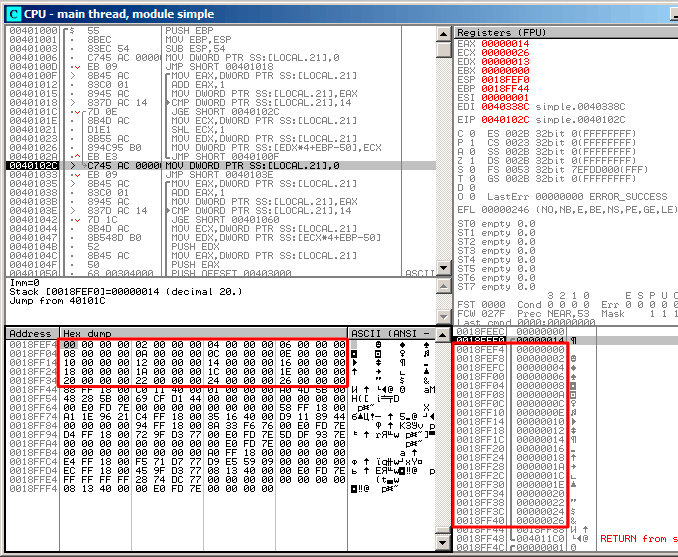
\includegraphics[scale=\FigScale]{patterns/13_arrays/1_simple/olly.png}
\caption{\olly: \RU{после заполнения массива}\EN{after array filling}}
\label{fig:array_simple_olly}
\end{figure}

\RU{А так как этот массив находится в стеке, то мы видим все его 20 элементов внутри стека.}
\EN{Since this array is located in the stack, we can see all its 20 elements there.}

\fi

\ifdefined\IncludeGCC
\subsubsection{GCC}

\RU{Рассмотрим результат работы GCC 4.4.1:}\EN{Here is what GCC 4.4.1 does:}

\lstinputlisting[caption=GCC 4.4.1]{patterns/13_arrays/1_simple/simple_gcc.asm}

\RU{Переменная $a$ в нашем примере имеет тип \IT{int*} (указатель на \Tint{}).
Вы можете попробовать передать в другую функцию указатель на массив,
но точнее было бы сказать, что передается указатель на первый элемент массива
(а адреса остальных элементов массива можно вычислить очевидным образом).}
\EN{By the way, variable $a$ is of type  \IT{int*} 
(the pointer to \Tint{})---you can pass a pointer to an array to another function,
but it's more correct to say that a pointer to the first element of the array is passed
(the addresses of rest of the elements are calculated in an obvious way).}
\RU{Если индексировать этот указатель как \IT{a[idx]}, \IT{idx} просто прибавляется к указателю 
и возвращается элемент, расположенный там, куда ссылается вычисленный указатель.}
\EN{If you index this pointer as \IT{a[idx]}, \IT{idx} is just to be added to the pointer 
and the element placed there (to which calculated pointer is pointing) is to be returned.}

\RU{Вот любопытный пример. Строка символов вроде \IT{\q{string}} это массив из символов. 
Она имеет тип \IT{const char[]}.}\EN{An interesting example: a string of characters like 
\IT{\q{string}} is an array of characters and it has a type of \IT{const char[]}.}
\RU{К этому указателю также можно применять индекс.}
\EN{An index can also be applied to this pointer.}
\RU{Поэтому можно написать даже так:  \TT{\q{string}[i]}~--- это совершенно легальное выражение в \CCpp!}
\EN{And that is why it is possible to write things like \TT{\q{string}[i]}---this is a correct \CCpp expression!}
\fi

\ifdefined\IncludeARM
\subsection{ARM}

\subsubsection{\NonOptimizingKeilVI (\ARMMode)}

\lstinputlisting{patterns/13_arrays/1_simple/simple_Keil_ARM_O0.asm.\LANG}

\RU{Тип \Tint требует 32 бита для хранения (или 4 байта),}
\EN{\Tint type requires 32 bits for storage (or 4 bytes),}
\RU{так что для хранения 20 переменных типа \Tint, нужно 80 (\TT{0x50}) байт.}
\EN{so to store 20 \Tint variables 80 (\TT{0x50}) bytes are needed.}
\RU{Поэтому инструкция}\EN{So that is why the} \INS{SUB SP, SP, \#0x50} 
\RU{в прологе функции выделяет в локальном стеке под массив именно столько места.}
\EN{instruction in the function's prologue allocates exactly this amount of space in the stack.}

\RU{И в первом и во втором цикле итератор цикла \var{i} будет постоянно находится в регистре \Reg{4}.}
\EN{In both the first and second loops, the loop iterator \var{i} is placed in the \Reg{4} register.}

\index{ARM!Optional operators!LSL}
\RU{Число, которое нужно записать в массив, вычисляется так: $i*2$, и это эквивалентно 
сдвигу на 1 бит влево, так что инструкция \INS{MOV R0, R4,LSL\#1} делает это.}
\EN{The number that is to be written into the array is calculated as $i*2$, which is effectively equivalent 
to shifting it left by one bit, so \INS{MOV R0, R4,LSL\#1} instruction does this.}

\index{ARM!\Instructions!STR}
\INS{STR R0, [SP,R4,LSL\#2]} \RU{записывает содержимое \Reg{0} в массив}\EN{writes the contents of \Reg{0} into the array}.
\RU{Указатель на элемент массива вычисляется так: \ac{SP} указывает на начало массива, \Reg{4} это $i$.}
\EN{Here is how a pointer to array element is calculated: \ac{SP} points to the start of the array, \Reg{4} is $i$.}
\RU{Так что сдвигаем $i$ на 2 бита влево, что эквивалентно умножению на 4 
(ведь каждый элемент массива занимает 4 байта) и прибавляем это к адресу начала массива.}
\EN{So shifting $i$ left by 2 bits is effectively equivalent to multiplication by 4
(since each array element has a size of 4 bytes) and then it's added to the address of the start of the array.}

\index{ARM!\Instructions!LDR}
\RU{Во втором цикле используется обратная инструкция \INS{LDR R2, [SP,R4,LSL\#2]}.
Она загружает из массива нужное значение и указатель на него вычисляется точно так же.}
\EN{The second loop has an inverse \INS{LDR R2, [SP,R4,LSL\#2]}
instruction. It loads the value we need from the array, and the pointer to it is calculated likewise.}

\subsubsection{\OptimizingKeilVI (\ThumbMode)}

\lstinputlisting{patterns/13_arrays/1_simple/simple_Keil_thumb_O3.asm.\LANG}

\RU{Код для Thumb очень похожий.}\EN{Thumb code is very similar.}
\index{ARM!\Instructions!LSLS}
\RU{В Thumb имеются отдельные инструкции для битовых сдвигов (как \TT{LSLS}), 
вычисляющие и число для записи в массив и адрес каждого элемента массива.}
\EN{Thumb mode has special instructions for bit shifting (like \TT{LSLS}),
which calculates the value to be written into the array and the address of each element in the array as well.}

\RU{Компилятор почему-то выделил в локальном стеке немного больше места, 
однако последние 4 байта не используются.}
\EN{The compiler allocates slightly more space in the local stack, however, the last 4 bytes are not used.}

\subsubsection{\NonOptimizing GCC 4.9.1 (ARM64)}

\lstinputlisting[caption=\NonOptimizing GCC 4.9.1 (ARM64)]{patterns/13_arrays/1_simple/ARM64_GCC491_O0.s.\LANG}

\fi
\ifdefined\IncludeMIPS
\subsection{MIPS}
% FIXME better start at non-optimizing version?
\RU{Функция использует много S-регистров, которые должны быть сохранены. Вот почему их значения сохраняются
в прологе функции и восстанавливаются в эпилоге.}
\EN{The function uses a lot of S- registers which must be preserved, so that's why its 
values are saved in the function prologue and restored in the epilogue.}

\lstinputlisting[caption=\Optimizing GCC 4.4.5 (IDA)]{patterns/13_arrays/1_simple/MIPS_O3_IDA.lst.\LANG}

\RU{Интересная вещь: здесь два цикла и в первом не нужна переменная $i$, а нужна только переменная
$i*2$ (скачущая через 2 на каждой итерации) и ещё адрес в памяти (скачущий через 4 на каждой итерации).}
\EN{Something interesting: there are two loops and the first one doesn't needs $i$, it needs only 
$i*2$ (increased by 2 at each iteration) and also the address in memory (increased by 4 at each iteration).}
\RU{Так что мы видим здесь две переменных: одна (в \$V0) увеличивается на 2 каждый раз, и вторая (в \$V1) --- 
на 4.}
\EN{So here we see two variables, one (in \$V0) increasing by 2 each time, and another (in \$V1) --- by 4.}

\RU{Второй цикл содержит вызов \printf. Он должен показывать значение $i$ пользователю,
поэтому здесь есть переменная, увеличивающаяся на 1 каждый раз (в \$S0), а также адрес в памяти (в \$S1) 
увеличивающийся на 4 каждый раз.}
\EN{The second loop is where \printf is called and it reports the value of $i$ to the user, 
so there is a variable
which is increased by 1 each time (in \$S0) and also a memory address (in \$S1) increased by 4 each time.}

\RU{Это напоминает нам оптимизацию циклов, которую мы рассматривали ранее:}
\EN{That reminds us of loop optimizations we considered earlier:} \myref{loop_iterators}.
\RU{Цель оптимизации в том, чтобы избавиться от операций умножения.}
\EN{Their goal is to get rid of of multiplications.}

\fi

\section{\RU{Переполнение буфера}\EN{Buffer overflow}}
\label{subsec:bufferoverflow}
\index{\BufferOverflow}

\subsection{\RU{Чтение за пределами массива}\EN{Reading outside array bounds}}

\RU{Итак, индексация массива\EMDASH{}это просто \IT{массив\lbrack{}индекс\rbrack}.  % TODO1 как-то плохо отображаются []
Если вы присмотритесь к коду, в цикле печати значений массива через \printf вы 
не увидите проверок индекса, \IT{меньше ли он двадцати?} 
А что будет если он будет 20 или больше? 
Эта одна из особенностей \CCpp, за которую их, собственно, и ругают.}
\EN{So, array indexing is just \IT{array\lbrack{}index\rbrack}.
If you study the generated code closely, you'll probably note the missing index bounds checking,
which could check \IT{if it is less than 20}.
What if the index is 20 or greater?
That's the one \CCpp feature it is often blamed for.}

\RU{Вот код, который и компилируется и работает:}
\EN{Here is a code that successfully compiles and works:}

\lstinputlisting{patterns/13_arrays/2_BO/r.c}

\RU{Вот результат компиляции в}\EN{Compilation results} (MSVC 2008):

\lstinputlisting[caption=\NonOptimizing MSVC 2008]{patterns/13_arrays/2_BO/r_msvc.asm}

\RU{Данный код при запуске выдал вот такой результат:}\EN{The code produced this result:}

\begin{figure}[h]
\centering
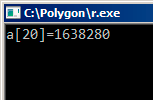
\includegraphics[scale=\NormalScale]{patterns/13_arrays/2_BO/olly_r3.png}
\caption{\olly: \RU{вывод в консоль}\EN{console output}}
\label{fig:array_BO_olly_r3}
\end{figure}

\RU{Это просто \IT{что-то}, что волею случая лежало в стеке рядом с массивом, 
через 80 байт от его первого элемента.}
\EN{It is just \IT{something} that was lying in the stack near to the array, 80 bytes away from its first element.}

\ifdefined\IncludeOlly
\clearpage
\index{\olly}
\RU{Попробуем узнать в \olly, что это за значение}\EN{Let's try to find out where did this value
come from, using \olly}.
\RU{Загружаем и находим это значение, находящееся точно после последнего элемента массива:}
\EN{Let's load and find the value located right after the last array element:}

\begin{figure}[H]
\centering
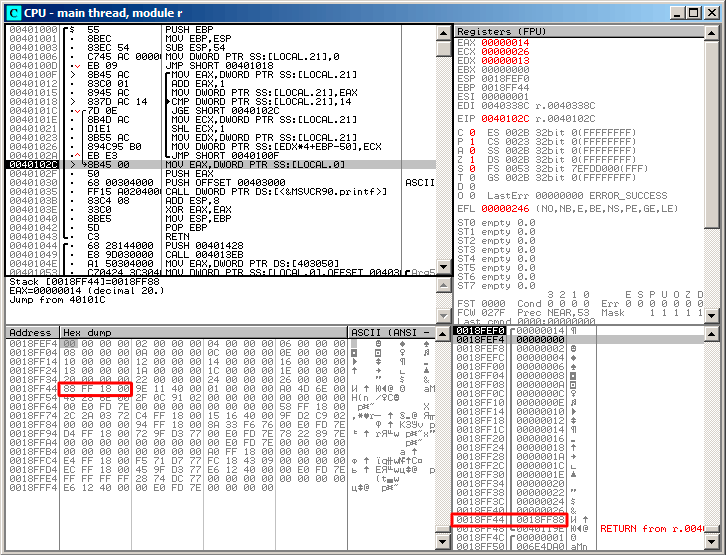
\includegraphics[scale=\FigScale]{patterns/13_arrays/2_BO/olly_r1.png}
\caption{\olly: \RU{чтение 20-го элемента и вызов \printf}\EN{reading of the 20th element and execution of \printf}}
\label{fig:array_BO_olly_r1}
\end{figure}

\RU{Что это за значение}\EN{What is this}? 
\RU{Судя по разметке стека, это сохраненное значение регистра EBP}\EN{Judging by the stack layout,
this is the saved value of the EBP register}.
\clearpage
\RU{Трассируем далее, и видим, как оно восстанавливается}\EN{Let's trace further and see how
it gets restored}:

\begin{figure}[H]
\centering
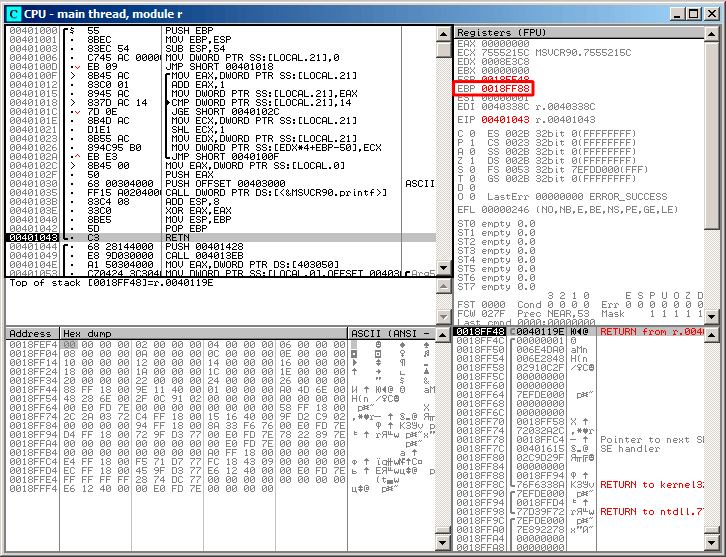
\includegraphics[scale=\FigScale]{patterns/13_arrays/2_BO/olly_r2.png}
\caption{\olly: \RU{восстановление EBP}\EN{restoring value of EBP}}
\label{fig:array_BO_olly_r2}
\end{figure}

\RU{Действительно, а как могло бы быть иначе? Компилятор мог бы встроить какой-то код, 
каждый раз проверяющий индекс на соответствие пределам массива, как в языках программирования 
более высокого уровня\footnote{Java, Python, \etc{}.}, что делало бы запускаемый код медленнее.}
\EN{Indeed, how it could be different?
The compiler may generate some additional code to check the index value to be always
in the array's bounds (like in higher-level programming languages\footnote{Java, Python, \etc{}})
but this makes the code slower.}

\fi

\subsection{\RU{Запись за пределы массива}\EN{Writing beyond array bounds}}

\RU{Итак, мы прочитали какое-то число из стека явно \IT{нелегально}, а что если мы запишем?}
\EN{OK, we read some values from the stack \IT{illegally}, but what if we could write something to it?}

\RU{Вот что мы пишем:}\EN{Here is what we have got:}

\lstinputlisting{patterns/13_arrays/2_BO/w.c}

\subsubsection{MSVC}

\RU{И вот что имеем на ассемблере:}\EN{And what we get:}

\lstinputlisting[caption=\NonOptimizing MSVC 2008]{patterns/13_arrays/2_BO/w.asm.\LANG}

\RU{Запускаете скомпилированную программу, и она падает. Немудрено. Но давайте теперь узнаем, где именно.}
\EN{The compiled program crashes after running. No wonder. Let's see where exactly does it is crash.}

\clearpage
\index{\olly}

\RU{Загружаем в}\EN{Let's load it into} \olly, \RU{трассируем пока запишутся все 30 элементов:}
\EN{and trace until all 30 elements are written:}

\begin{figure}[H]
\centering
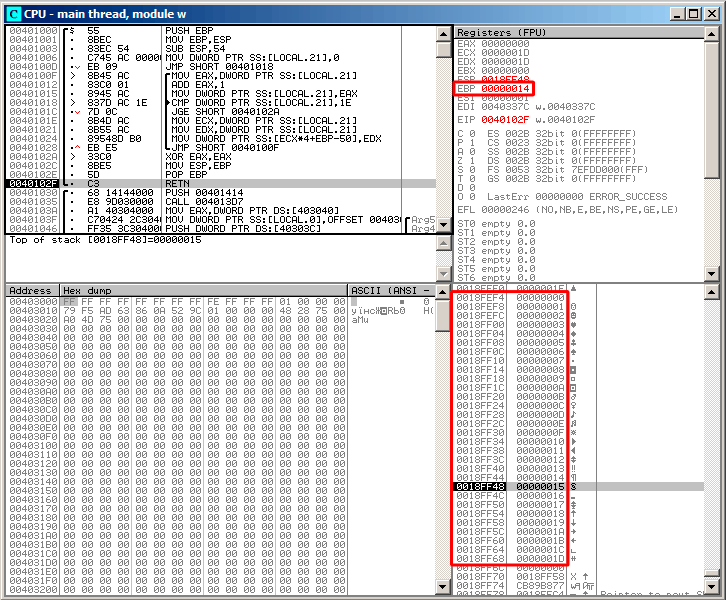
\includegraphics[scale=\FigScale]{patterns/13_arrays/2_BO/olly_w1.png}
\caption{\olly: \RU{после восстановления EBP}\EN{after restoring the value of EBP}}
\label{fig:array_BO_olly_w1}
\end{figure}

\clearpage
\RU{Доходим до конца функции}\EN{Trace until the function end}:

\begin{figure}[H]
\centering
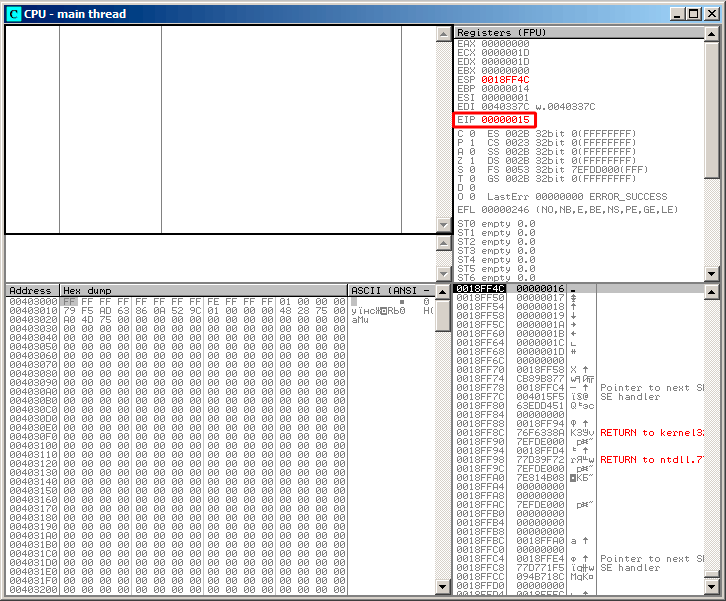
\includegraphics[scale=\FigScale]{patterns/13_arrays/2_BO/olly_w2.png}
\caption{\olly: \RU{EIP восстановлен, но \olly не может дизассемблировать по адресу 0x15}
\EN{EIP was restored, but \olly can't disassemble at 0x15}}
\label{fig:array_BO_olly_w2}
\end{figure}

\RU{Итак, следите внимательно за регистрами.}
\EN{Now please keep your eyes on the registers.}

\RU{\EIP теперь 0x15. Это явно нелегальный адрес для кода~--- по крайней мере, win32-кода! 
Мы там как-то очутились, причем, сами того не хотели. Интересен также тот факт, что в \EBP хранится 0x14, 
а в \ECX и \EDX~--- 0x1D.}
\EN{\EIP is 0x15 now. It is not a legal address for code---at least for win32 code!
We got there somehow against our will.
It is also interesting that the \EBP register contain 0x14,
\ECX and \EDX---0x1D.}

\RU{Ещё немного изучим разметку стека.}\EN{Let's study stack layout a bit more.}

\RU{После того как управление передалось в \main, в стек было сохранено значение \EBP. 
Затем для массива и переменной $i$ было выделено 84 байта. Это \TT{(20+1)*sizeof(int)}. 
\ESP сейчас указывает на переменную \TT{\_i} в локальном стеке и при исполнении следующего \INS{PUSH что-либо}, 
\IT{что-либо} появится рядом с \TT{\_i}.}
\EN{After the control flow was passed to \TT{\main}, the value in the \EBP register was saved on the stack.
Then, 84 bytes were allocated for the array and the $i$ variable.
That's \TT{(20+1)*sizeof(int)}.
\ESP now points to the \TT{\_i} variable in the local stack and after the execution of 
the next \TT{PUSH something}, \IT{something} is appearing next to \TT{\_i}.}

\RU{Вот так выглядит разметка стека пока управление находится внутри}
\EN{That's the stack layout while the control is in} \main:

\begin{center}
\begin{tabular}{ | l | l | }
\hline
  \TT{ESP}    & \RU{4 байта выделенных для переменной $i$}\EN{4 bytes allocated for $i$ variable} \\
\hline
  \TT{ESP+4}  & \RU{80 байт выделенных для массива \TT{a[20]}}\EN{80 bytes allocated for \TT{a[20]} array} \\
\hline
  \TT{ESP+84} & \RU{сохраненное значение \EBP}\EN{saved \EBP value} \\
\hline
  \TT{ESP+88} & \RU{адрес возврата}\EN{return address} \\
\hline
\end{tabular}
\end{center}

\RU{Выражение \TT{a[19]=что\_нибудь} записывает последний \Tint в пределах массива (пока что в пределах!)}
\EN{\TT{a[19]=something} statement writes the last \Tint in the bounds of the array (in bounds so far!)}

\RU{Выражение \TT{a[20]=что\_нибудь} записывает \IT{что\_нибудь} на место где сохранено значение \EBP.}
\EN{\TT{a[20]=something} statement writes \IT{something} to the place where the value of \EBP is saved.}

\RU{Обратите внимание на состояние регистров на момент падения процесса. В нашем случае 
в 20-й элемент записалось значение 20. 
И вот всё дело в том, что заканчиваясь, эпилог функции восстанавливал значение \EBP 
(20 в десятичной системе это как раз \TT{0x14} в шестнадцатеричной). 
Далее выполнилась инструкция \RET, которая на самом деле эквивалентна \TT{POP EIP}.}
\EN{Please take a look at the register state at the moment of the crash. In our case,
20 was written in the 20th element. 
At the function end, the function epilogue restores the original \EBP value.
(20 in decimal is \TT{0x14} in hexadecimal).
Then \RET gets executed, which is effectively equivalent to \TT{POP EIP} instruction.}

\RU{Инструкция \RET вытащила из стека адрес возврата (это адрес где-то внутри \ac{CRT}), 
которая вызвала \main), 
а там было записано 21 в десятичной системе, то есть 0x15 в шестнадцатеричной. 
И вот процессор оказался по адресу 0x15, но исполняемого кода там нет, так что случилось исключение.}
\EN{The \RET instruction takes the return address from the stack (that is the address in \ac{CRT}),
which was called \main),
and 21 iss stored there (\TT{0x15} in hexadecimal).
The CPU traps at address \TT{0x15},
but there is no executable code there, so exception gets raised.}

\index{\RU{Переполнение буфера}\EN{Buffer overflow}}
\RU{Добро пожаловать! Это называется}
\EN{Welcome! It is called a} \IT{buffer overflow}\footnote{\href{http://go.yurichev.com/17132}{wikipedia}}.

\RU{Замените массив \Tint на строку (массив \Tchar), нарочно создайте слишком длинную строку, 
передайте её в ту программу, 
в ту функцию, которая не проверяя длину строки скопирует её в слишком короткий буфер, 
и вы сможете указать программе, по какому именно адресу перейти. 
Не всё так просто в реальности, конечно, но началось всё с этого%
\footnote{Классическая статья об этом: \cite{Phrack4914}}.}
\EN{Replace the \Tint array with a string (\Tchar array), create a long string deliberately
and pass it to the program, to the function, which doesn't check the length of the string and copies it in a short buffer,
and you'll able to point the program to an address to which it must jump.
It's not that simple in reality, but that is how it emerged%
\footnote{Classic article about it: \cite{Phrack4914}.}}

\ifdefined\IncludeGCC
\subsubsection{GCC}

\RU{Попробуем то же самое в GCC 4.4.1. У нас выходит такое:}
\EN{Let's try the same code in GCC 4.4.1. We get:}

\lstinputlisting{patterns/13_arrays/2_BO/w_gcc.asm}

\RU{Запуск этого в Linux выдаст:}\EN{Running this in Linux will produce:} \TT{Segmentation fault}.

\index{GDB}
\RU{Если запустить полученное в отладчике GDB, получим:}
\EN{If we run this in the GDB debugger, we get this:}

\begin{lstlisting}
(gdb) r
Starting program: /home/dennis/RE/1 

Program received signal SIGSEGV, Segmentation fault.
0x00000016 in ?? ()
(gdb) info registers
eax            0x0	0
ecx            0xd2f96388	-755407992
edx            0x1d	29
ebx            0x26eff4	2551796
esp            0xbffff4b0	0xbffff4b0
ebp            0x15	0x15
esi            0x0	0
edi            0x0	0
eip            0x16	0x16
eflags         0x10202	[ IF RF ]
cs             0x73	115
ss             0x7b	123
ds             0x7b	123
es             0x7b	123
fs             0x0	0
gs             0x33	51
(gdb) 
\end{lstlisting}

\RU{Значения регистров немного другие, чем в примере win32, потому что разметка стека чуть другая.}
\EN{The register values are slightly different than in win32 example, 
since the stack layout is slightly different too.}
\fi


\ifx\LITE\undefined
\section{\RU{Защита от переполнения буфера}\EN{Buffer overflow protection methods}}
\label{subsec:BO_protection}

\RU{В наше время пытаются бороться с переполнением буфера невзирая на халатность программистов на \CCpp. 
В MSVC есть опции вроде}%
\EN{There are several methods to protect against this scourge, regardless of the \CCpp programmers' negligence.
MSVC has options like}\footnote{
\RU{описания защит, которые компилятор может вставлять в код}%
\EN{compiler-side buffer overflow protection methods}:
\href{http://go.yurichev.com/17133}{wikipedia.org/wiki/Buffer\_overflow\_protection}}:

\begin{lstlisting}
 /RTCs Stack Frame runtime checking
 /GZ Enable stack checks (/RTCs)
\end{lstlisting}

\index{x86!\Instructions!RET}
\index{Function prologue}
\index{Security cookie}
\RU{Одним из методов является вставка в прологе функции некоего случайного значения в область локальных переменных 
и проверка этого значения в эпилоге функции перед выходом. 
Если проверка не прошла, то не выполнять инструкцию \RET, а остановиться (или зависнуть). 
Процесс зависнет, но это лучше, чем удаленная атака на ваш компьютер.}
\EN{One of the methods is to write a random value between the local variables in stack at function prologue 
and to check it in function epilogue before the function exits.
If value is not the same, do not execute the last instruction \RET, but stop (or hang).
The process will halt, but that is much better than a remote attack to your host.}
    
\newcommand{\CANARYURL}{\RU{\href{http://go.yurichev.com/17135}{miningwiki.ru/wiki/Канарейка\_в\_шахте}}%
\EN{\href{http://go.yurichev.com/17134}{wikipedia.org/wiki/Domestic\_canary\#Miner.27s\_canary}}}

\index{Canary}
\RU{Это случайное значение иногда называют \q{канарейкой}%
\footnote{\q{canary} в англоязычной литературе}, 
по аналогии с шахтной канарейкой\footnote{\CANARYURL}.
Раньше использовали шахтеры, чтобы определять, есть ли в шахте опасный газ.
}
\EN{This random value is called a \q{canary} sometimes, it is related to the miners' canary\footnote{\CANARYURL},
they were used by miners in the past days in order to detect poisonous gases quickly.}
\RU{Канарейки очень к нему чувствительны и либо проявляли сильное беспокойство, либо гибли от газа.}
\EN{Canaries are very sensitive to mine gases, they become very agitated in case of danger, or even die.}

\RU{Если скомпилировать наш простейший пример работы с массивом}
\EN{If we compile our very simple array example}~(\myref{arrays_simple}) \InENRU \ac{MSVC}
\RU{с опцией RTC1 или RTCs}\EN{with RTC1 and RTCs option}, \RU{в конце нашей функции будет вызов 
функции}\EN{you can see a call to}
\TT{@\_RTC\_CheckStackVars@8}\RU{, проверяющей корректность \q{канарейки}.}
\EN{ a function at the end of the function that checks if the \q{canary} is correct.}

\RU{Посмотрим, как дела обстоят в GCC}\EN{Let's see how GCC handles this}. 
\RU{Возьмем пример из секции про}\EN{Let's take an} \TT{alloca()}~(\myref{alloca})\EN{ example}:

\lstinputlisting{patterns/02_stack/04_alloca/2_1.c}

\RU{По умолчанию, без дополнительных ключей, GCC 4.7.3 вставит в код проверку \q{канарейки}:}
\EN{By default, without any additional options, GCC 4.7.3 inserts a \q{canary} check into the code:}

\lstinputlisting[caption=GCC 4.7.3]{patterns/13_arrays/3_BO_protection/gcc_canary.asm.\LANG}

\index{x86!\Registers!GS}
\RU{Случайное значение находится в}\EN{The random value is located in} \TT{gs:20}. 
\RU{Оно записывается в стек, затем, в конце функции, значение в стеке
сравнивается с корректной \q{канарейкой} в}\EN{It gets written on the stack and then at the end of the function
the value in the stack is compared with the correct \q{canary} in} \TT{gs:20}. 
\RU{Если значения не равны, будет вызвана функция}\EN{If the values are not equal, the} 
\TT{\_\_stack\_chk\_fail} \RU{и в консоли мы увидим что-то вроде такого}
\EN{function is called and we can see in the console something like that} (Ubuntu 13.04 x86):

\begin{lstlisting}
*** buffer overflow detected ***: ./2_1 terminated
======= Backtrace: =========
/lib/i386-linux-gnu/libc.so.6(__fortify_fail+0x63)[0xb7699bc3]
/lib/i386-linux-gnu/libc.so.6(+0x10593a)[0xb769893a]
/lib/i386-linux-gnu/libc.so.6(+0x105008)[0xb7698008]
/lib/i386-linux-gnu/libc.so.6(_IO_default_xsputn+0x8c)[0xb7606e5c]
/lib/i386-linux-gnu/libc.so.6(_IO_vfprintf+0x165)[0xb75d7a45]
/lib/i386-linux-gnu/libc.so.6(__vsprintf_chk+0xc9)[0xb76980d9]
/lib/i386-linux-gnu/libc.so.6(__sprintf_chk+0x2f)[0xb7697fef]
./2_1[0x8048404]
/lib/i386-linux-gnu/libc.so.6(__libc_start_main+0xf5)[0xb75ac935]
======= Memory map: ========
08048000-08049000 r-xp 00000000 08:01 2097586    /home/dennis/2_1
08049000-0804a000 r--p 00000000 08:01 2097586    /home/dennis/2_1
0804a000-0804b000 rw-p 00001000 08:01 2097586    /home/dennis/2_1
094d1000-094f2000 rw-p 00000000 00:00 0          [heap]
b7560000-b757b000 r-xp 00000000 08:01 1048602    /lib/i386-linux-gnu/libgcc_s.so.1
b757b000-b757c000 r--p 0001a000 08:01 1048602    /lib/i386-linux-gnu/libgcc_s.so.1
b757c000-b757d000 rw-p 0001b000 08:01 1048602    /lib/i386-linux-gnu/libgcc_s.so.1
b7592000-b7593000 rw-p 00000000 00:00 0
b7593000-b7740000 r-xp 00000000 08:01 1050781    /lib/i386-linux-gnu/libc-2.17.so
b7740000-b7742000 r--p 001ad000 08:01 1050781    /lib/i386-linux-gnu/libc-2.17.so
b7742000-b7743000 rw-p 001af000 08:01 1050781    /lib/i386-linux-gnu/libc-2.17.so
b7743000-b7746000 rw-p 00000000 00:00 0
b775a000-b775d000 rw-p 00000000 00:00 0
b775d000-b775e000 r-xp 00000000 00:00 0          [vdso]
b775e000-b777e000 r-xp 00000000 08:01 1050794    /lib/i386-linux-gnu/ld-2.17.so
b777e000-b777f000 r--p 0001f000 08:01 1050794    /lib/i386-linux-gnu/ld-2.17.so
b777f000-b7780000 rw-p 00020000 08:01 1050794    /lib/i386-linux-gnu/ld-2.17.so
bff35000-bff56000 rw-p 00000000 00:00 0          [stack]
Aborted (core dumped)
\end{lstlisting}

\index{MS-DOS}
gs \RU{это так называемый сегментный регистр. Эти регистры широко использовались во времена MS-DOS 
и DOS-экстендеров.}\EN{is the so-called segment register. These registers were used widely in MS-DOS and DOS-extenders
times.}
\RU{Сейчас их функция немного изменилась.}\EN{Today, its function is different.}
\index{TLS}
\index{Windows!TIB}
\RU{Если говорить кратко, в Linux \TT{gs} всегда указывает на \ac{TLS}~(\myref{TLS})~--- там находится различная 
информация, специфичная для выполняющегося потока.}
\EN{To say it briefly, the \TT{gs} register in Linux always points to the
\ac{TLS}~(\myref{TLS})---some information specific to thread is stored there.}
\RU{Кстати, в win32 эту же роль играет сегментный регистр \TT{fs},
он всегда указывает на}\EN{By the way, in win32
the \TT{fs} register plays the same role, pointing to}
\ac{TIB} \footnote{\href{http://go.yurichev.com/17104}{wikipedia.org/wiki/Win32\_Thread\_Information\_Block}}. 

\RU{Больше информации можно почерпнуть из исходных кодов Linux (по крайней мере, в версии 3.11): 
в файле}\EN{More information can be found in the Linux kernel source code (at least in 3.11 version), in}
\IT{arch/x86/include/asm/stackprotector.h}\RU{ в комментариях описывается эта переменная.}
\EN{ this variable is described in the comments.}

\ifdefined\IncludeARM
\subsection{\OptimizingXcodeIV (\ThumbTwoMode)}

\RU{Возвращаясь к нашему простому примеру}
\EN{Let's get back to our simple array example} (\myref{arrays_simple}),
\RU{можно посмотреть, как LLVM добавит проверку \q{канарейки}:}
\EN{again, now we can see how LLVM checks the correctness of the \q{canary}:}

% TODO shorten the listing a bit? is full display of unrolled loop necessary?
\lstinputlisting{patterns/13_arrays/3_BO_protection/simple_Xcode_thumb_O3.asm.\LANG}

\index{Unrolled loop}
\RU{Во-первых, LLVM \q{развернул} цикл и все значения записываются в массив по одному, 
уже вычисленные, 
потому что LLVM посчитал что так будет быстрее.}
\EN{First of all, as we see, LLVM \q{unrolled} the loop and all values were written into an array one-by-one,
pre-calculated, as LLVM concluded it can work faster.}
\RU{Кстати, инструкции режима ARM позволяют сделать это ещё быстрее и это может быть вашим 
домашним заданием.}\EN{By the way, instructions in ARM mode may help to do this even faster, 
and finding this could be your homework.}

\RU{В конце функции мы видим сравнение \q{канареек}~--- той что лежит в локальном стеке и корректной, 
на которую ссылается регистр \Reg{8}.}
\EN{At the function end we see the comparison of the \q{canaries}---the one in the local stack and the correct one,
to which \Reg{8} points.}
\index{ARM!\Instructions!IT}
\RU{Если они равны, срабатывает блок из четырех инструкций при помощи \INS{ITTTT EQ}.
Это запись 0 в \Reg{0}, эпилог функции и выход из нее.}
\EN{If they are equal to each other, a 4-instruction block is triggered by \INS{ITTTT EQ},
which contains writing 0 in \Reg{0}, the function epilogue and exit.}
\RU{Если \q{канарейки} не равны, блок не срабатывает и происходит
переход на функцию}\EN{If the \q{canaries} are not equal, the block being skipped,
and the jump to} \TT{\_\_\_stack\_chk\_fail}\RU{, которая, вероятно, остановит работу программы.}
\EN{ function will occur, which, perhaps, will halt execution.}
% TODO1 illustrate this!

\fi

\fi
\section{\RU{Еще немного о массивах}\EN{One more word about arrays}}

\RU{Теперь понятно, почему нельзя написать в исходном коде на \CCpp что-то вроде:}
\EN{Now we understand why it is impossible to write something like this in \CCpp code:}

\begin{lstlisting}
void f(int size)
{
    int a[size];
...
};
\end{lstlisting}

\RU{Чтобы выделить место под массив в локальном стеке, 
компилятору нужно знать размер массива, чего он на стадии компиляции, 
разумеется, знать не может.}
\EN{That's just because the compiler must know the exact array size to allocate space for 
it in the local stack layout on at the compiling stage.}

\index{\CLanguageElements!C99!variable length arrays}
\index{\CStandardLibrary!alloca()}
\RU{Если вам нужен массив произвольной длины, то выделите столько, сколько нужно, через \TT{malloc()}, 
а затем обращайтесь к выделенному блоку байт как к массиву того типа, который вам нужен.}
\EN{If you need an array of arbitrary size, allocate it by using \TT{malloc()}, then access the allocated memory block
as an array of variables of the type you need.}

\RU{Либо используйте возможность стандарта C99~\cite[6.7.5/2]{C99TC3}, 
и внутри это очень похоже на alloca()~(\myref{alloca}).}
\EN{Or use the C99 standard feature\cite[6.7.5/2]{C99TC3}, 
and it works like alloca()~(\myref{alloca}) internally.}

\RU{Для работы в с памятью, можно также воспользоваться библиотекой сборщика мусора в Си.}
\EN{It's also possible to use garbage collecting libraries for C.}
\RU{А для языка Си++ есть библиотеки с поддержкой умных указателей.}
\EN{And there are also libraries supporting smart pointers for C++.}


\section{\RU{Массив указателей на строки}\EN{Array of pointers to strings}}
\label{array_of_pointers_to_strings}

\RU{Вот пример массива указателей.}\EN{Here is an example for an array of pointers.}

\lstinputlisting[caption=\RU{Получить имя месяца}\EN{Get month name},label=get_month1]{patterns/13_arrays/45_month_1D/month1.c.\LANG}

\subsection{x64}

\lstinputlisting[caption=\Optimizing MSVC 2013 x64]{patterns/13_arrays/45_month_1D/month1_MSVC_2013_x64_Ox.asm}

\RU{Код очень простой}\EN{The code is very simple}:

\begin{itemize}

\item
\index{x86!\Instructions!MOVSXD}
\RU{Первая инструкция \INS{MOVSXD} копирует 32-битное значение из \ECX (где передается аргумент :$month$)
в \RAX с знаковым расширением (потому что аргумент $month$ имеет тип \Tint).}
\EN{The first \INS{MOVSXD} instruction copies a 32-bit value from \ECX (where $month$ argument is passed) 
to \RAX with sign-extension (because the $month$ argument is of type \Tint).}
\RU{Причина расширения в том, что это значение будет использоваться в вычислениях наряду с другими 64-битными
значениями.}
\EN{The reason for the sign extension is that this 32-bit value is to be used in calculations
with other 64-bit values.}
\RU{Таким образом, оно должно быть расширено до 64-битного}%
\EN{Hence, it has to be promoted to 64-bit}%
\footnote{\RU{Это немного странная вещь, но отрицательный индекс массива может быть передан как $month$ 
\ifx\LITE\undefined
(отрицательные индексы массивов будут рассмотрены позже: \myref{negative_array_indices})
\fi
. И если так будет, отрицательное значение типа \Tint будет расширено со знаком корректно
и соответствующий элемент перед таблицей будет выбран.
Всё это не будет корректно работать без знакового расширения.}
\EN{It is somewhat weird, but negative array index could be passed here as $month$
\ifx\LITE\undefined
(negative array indices will have been explained later: \myref{negative_array_indices}) 
\fi
. And if this happens, the negative input value of \Tint type is sign-extended correctly 
and the corresponding element before table is picked. 
It is not going to work correctly without sign-extension.}}.

\item
\RU{Затем адрес таблицы указателей загружается в \RCX.}
\EN{Then the address of the pointer table is loaded into \RCX.}

\item
\RU{В конце концов, входное значение ($month$) умножается на 8 и прибавляется к адресу.}
\EN{Finally, the input value ($month$) is multiplied by 8 and added to the address.}
\RU{Действительно: мы в 64-битной среде и все адреса (или указатели) 
требуют для хранения именно 64 бита (или 8 байт).}
\EN{Indeed: we are in a 64-bit environment and all address (or pointers) require exactly 64 bits (or 8 bytes) 
for storage.}
\RU{Следовательно, каждый элемент таблицы имеет ширину в 8 байт.}
\EN{Hence, each table element is 8 bytes wide.}
\RU{Вот почему для выбора элемента под нужным номером нужно пропустить $month*8$ байт от начала.}
\EN{And that's why to pick a specific element, $month*8$ bytes has to be skipped from the start.}
\RU{Это то, что делает \MOV}\EN{That's what \MOV does}.
\RU{Эта инструкция также загружает элемент по этому адресу.}
\EN{In addition, this instruction also loads the element at this address.}
\RU{Для 1, элемент будет указателем на строку, содержащую \q{February}, \etc.}
\EN{For 1, an element would be a pointer to a string that contains \q{February}, \etc.}

\end{itemize}

\Optimizing GCC 4.9 \RU{может это сделать даже лучше}\EN{can do the job even better}%
\footnote{\RU{В листинге осталось \q{0+}, потому что вывод ассемблера GCC не так скрупулёзен, чтобы убрать это.}
\EN{\q{0+} was left in the listing because GCC assembler output is not tidy enough to eliminate it.}
\RU{Это \IT{displacement} и он здесь нулевой.}\EN{It's \IT{displacement}, and it's zero here.}}:

\begin{lstlisting}[caption=\Optimizing GCC 4.9 x64]
	movsx	rdi, edi
	mov	rax, QWORD PTR month1[0+rdi*8]
	ret
\end{lstlisting}

\subsubsection{32-bit MSVC}

\RU{Скомпилируем также в 32-битном компиляторе MSVC:}\EN{Let's also compile it in the 32-bit MSVC compiler:}

\lstinputlisting[caption=\Optimizing MSVC 2013 x86]{patterns/13_arrays/45_month_1D/month1_MSVC_2013_x86_Ox.asm}

\RU{Входное значение не нужно расширять до 64-битного значения, так что оно используется как есть.}
\EN{The input value does not need to be extended to 64-bit value, so it is used as is.}
\RU{И оно умножается на 4, потому что элементы таблицы имеют ширину 32 бита или 4 байта.}
\EN{And it's multiplied by 4, because the table elements are 32-bit (or 4 bytes) wide.}

\ifdefined\IncludeARM
% FIXME1 move to another file
\subsection{32-\RU{битный}\EN{bit} ARM}

\subsubsection{ARM \RU{в режиме ARM}\EN{in ARM mode}}

\lstinputlisting[caption=\OptimizingKeilVI (\ARMMode)]{patterns/13_arrays/45_month_1D/month1_Keil_ARM_O3.s}

% TODO Fix R1s
\RU{Адрес таблицы загружается в R1.}
\EN{The address of the table is loaded in R1.}
\index{ARM!\Instructions!LDR}
\RU{Всё остальное делается, используя только одну инструкцию \LDR.}
\EN{All the rest is done using just one \LDR instruction.}
\RU{Входное значение $month$ сдвигается влево на 2 (что тоже самое что и умножение на 4), это значение
прибавляется к R1 (где находится адрес таблицы) и затем элемент таблицы загружается по этому адресу.}
\EN{Then input value $month$ is shifted left by 2 (which is the same as multiplying by 4), then added
to R1 (where the address of the table is) and then a table element is loaded from this address.}
\RU{32-битный элемент таблицы загружается в R0 из таблицы.}
\EN{The 32-bit table element is loaded into R0 from the table.}

\subsubsection{ARM \RU{в режиме Thumb}\EN{in Thumb mode}}

\RU{Код почти такой же, только менее плотный, потому что здесь, в инструкции \LDR, нельзя задать суффикс \LSL:}
\EN{The code is mostly the same, but less dense, because the \LSL suffix cannot be specified in the \LDR instruction here:}

\begin{lstlisting}
get_month1 PROC
        LSLS     r0,r0,#2
        LDR      r1,|L0.64|
        LDR      r0,[r1,r0]
        BX       lr
        ENDP
\end{lstlisting}

\subsection{ARM64}

\lstinputlisting[caption=\Optimizing GCC 4.9 ARM64]{patterns/13_arrays/45_month_1D/month1_GCC49_ARM64_O3.s}

\index{ARM!\Instructions!ADRP/ADD pair}
\RU{Адрес таблицы загружается в X1 используя пару \ADRP/\ADD.}
\EN{The address of the table is loaded in X1 using \ADRP/\ADD pair.}
\RU{Соответствующий элемент выбирается используя одну инструкцию \LDR, которая берет W0
(регистр, где находится значение входного аргумента $month$), сдвигает его на 3 бита влево
(что то же самое что и умножение на 8),
расширяет его, учитывая знак (это то, что означает суффикс \q{sxtw}) и прибавляет к X0.}
\EN{Then corresponding element is picked using just one \LDR, which takes W0 
(the register where input argument $month$ is), shifts it 3 bits to the left (which is the same as multiplying by 8), 
sign-extends it (this is what \q{sxtw} suffix implies) and adds to X0.}
\RU{Затем 64-битное значение загружается из таблицы в X0.}\EN{Then the 64-bit value is loaded from the table into X0.}
\fi

\ifdefined\IncludeMIPS
\subsection{MIPS}

\lstinputlisting[caption=\Optimizing GCC 4.4.5 (IDA)]{patterns/13_arrays/45_month_1D/MIPS_O3_IDA.lst.\LANG}
\fi

\ifx\LITE\undefined
\subsection{\RU{Переполнение массива}\EN{Array overflow}}

\RU{Наша функция принимает значения в пределах 0..11, но что будет, если будет передано 12?}
\EN{Our function accepts values in the range of 0..11, but what if 12 is passed?}
\RU{В таблице в этом месте нет элемента.}\EN{There is no element in table at this place.}
\RU{Так что функция загрузит какое-то значение, которое волею случая находится там, и вернет его.}
\EN{So the function will load some value which happens to be there, and return it.}
\RU{Позже, какая-то другая функция попытается прочитать текстовую строку по этому адресу и, возможно, упадет.}
\EN{Soon after, some other function can try to get a text string from this address and may crash.}

\RU{Скомпилируем этот пример в MSVC для win64 и откроем его в \IDA чтобы посмотреть, что линкер расположил
после таблицы:}%
\EN{Let's compile the example in MSVC for win64 and open it in \IDA to see what the linker has placed after the table:}

\lstinputlisting[caption=\RU{Исполняемый файл в}\EN{Executable file in} IDA]{patterns/13_arrays/45_month_1D/MSVC2012_win64_1.lst}

\RU{Имена месяцев идут сразу после.}\EN{Month names are came right after.}
\RU{Наша программа все-таки крошечная,
так что здесь не так уж много данных (всего лишь названия месяцев) для расположения их в сегменте данных.}
\EN{Our program is tiny, so there isn't much data to pack in the data segment, 
so it just the month names.}
\RU{Но нужно заметить, что там может быть действительно \emph{что угодно}, что линкер решит там расположить, случайным образом.}%
\EN{But it should be noted that there might be really \emph{anything} that linker has decided to put by chance.}

\RU{Так что будет если 12 будет передано в функцию?}\EN{So what if 12 is passed to the function?}
\RU{Вернется 13-й элемент таблицы}\EN{The 13th element will be returned}.
\RU{Посмотрим, как CPU обходится с байтами как с 64-битным значением:}
\EN{Let's see how the CPU treats the bytes there as a 64-bit value:}

\lstinputlisting[caption=\RU{Исполняемый файл в}\EN{Executable file in} IDA]{patterns/13_arrays/45_month_1D/MSVC2012_win64_2.lst}

\RU{И это}\EN{And this is} 0x797261756E614A.
\RU{После этого, какая-то другая функция (вероятно, работающая со строками) попытается загружать байты
по этому адресу, ожидая найти там Си-строку.}
\EN{Soon after, some other function (presumably, one that processes strings) may try to read bytes at 
this address, expecting a C-string there.}
\RU{И скорее всего упадет, потому что это значение не выглядит как действительный адрес.}
\EN{Most likely it is about to crash, because this value does't look like a valid address.}

\subsubsection{\RU{Защита от переполнения массива}\EN{Array overflow protection}}
\epigraph{
	\RU{Если какая-нибудь неприятность может случиться, она случается}
	\EN{If something can go wrong, it will}
	\ESph{}\PTBRph{}\PLph{}
}
{
	\RU{Закон Мерфи}
	\EN{Murphy's Law}
	\ESph{}\PTBRph{}\PLph{}
}

\RU{Немного наивно ожидать что всякий программист, кто будет использовать вашу функцию или библиотеку,
никогда не передаст аргумент больше 11.}
\EN{It's a bit naïve to expect that every programmer who use your function or library will never pass
an argument larger than 11.}
\RU{Существует также хорошая философия \q{fail early and fail loudly} или \q{fail-fast},
которая учит сообщать об ошибках как можно раньше и останавливаться.}
\EN{There exists the philosophy that says \q{fail early and fail loudly} or \q{fail-fast}, 
which teaches to report problems as early as possible and stop.}
\index{\CStandardLibrary!assert()}
\RU{Один из таких методов в \CCpp это макрос assert().}
\EN{One such method in \CCpp is assertions.}
\RU{Мы можем немного изменить нашу программу, чтобы она падала при передаче неверного значения:}
\EN{We can modify our program to fail if an incorrect value is passed:}

\lstinputlisting[caption=assert() \RU{добавлен}\EN{added}]{patterns/13_arrays/45_month_1D/month1_assert.c}

\RU{Макрос будет проверять на верные значения во время каждого старта функции и падать если выражение возвращает false.}
\EN{The assertion macro checks for valid values at every function start and fails if the expression is false.}

\lstinputlisting[caption=\Optimizing MSVC 2013 x64]{patterns/13_arrays/45_month_1D/MSVC2013_x64_Ox_checked.asm}

\RU{На самом деле, assert() это не функция, а макрос. Он проверяет условие и передает также номер строки и название
файла в другую функцию, которая покажет эту информацию пользователю.}
\EN{In fact, assert() is not a function, but macro. It checks for a condition, then passes also the line number and file
name to another function which reports this information to the user.}
\RU{Мы видим, что здесь и имя файла и выражение закодировано в UTF-16.}
\EN{Here we see that both file name and condition are encoded in UTF-16.}
\RU{Номер строки также передается (это 29)}\EN{The line number is also passed (it's 29)}.

\RU{Этот механизм, пожалуй, одинаковый во всех компиляторах.}
\EN{This mechanism is probably the same in all compilers.}
\RU{Вот что делает GCC}\EN{Here is what GCC does}:

\lstinputlisting[caption=\Optimizing GCC 4.9 x64]{patterns/13_arrays/45_month_1D/GCC491_x64_O3_checked.s}

\RU{Так что макрос в GCC также передает и имя функции, для удобства.}
\EN{So the macro in GCC also passes the function name for convenience.}

\RU{Ничего не бывает бесплатным и проверки на корректность тоже.}
\EN{Nothing is really free, and this is true for the sanitizing checks as well.}
\RU{Это может замедлить работу вашей программы, особенно если макрос assert() используется в маленькой
критичной ко времени функции.}
\EN{They make your program slower, especially if the assert() macros used in small time-critical functions.}
\RU{Так что, например, MSVC оставляет проверки в отладочных сборках, но в окончательных сборках они исчезают.}
\EN{So MSVC, for example, leaves the checks in debug builds, but in release builds they all disappear.}
 
\RU{Ядра Microsoft \gls{Windows NT} также идут в виде сборок \q{checked} и \q{free}}%
\EN{Microsoft \gls{Windows NT} kernels come in \q{checked} and \q{free} builds}%
\footnote{\href{http://go.yurichev.com/17259}{msdn.microsoft.com/en-us/library/windows/hardware/ff543450(v=vs.85).aspx}}.
\RU{В первых есть проверки на корректность аргументов (отсюда \q{checked}), а во вторых~--- нет (отсюда \q{free},
т.е.~\q{свободные} от проверок).}
\EN{The first has validation checks (hence, \q{checked}), the second one doesn't (hence, \q{free} of checks).}

% FIXME: ARM? MIPS?
\fi

\section{\RU{Многомерные массивы}\EN{Multidimensional arrays}}

\RU{Внутри многомерный массив выглядит так же как и линейный.}
\EN{Internally, a multidimensional array is essentially the same thing as a linear array.}
\RU{Ведь память компьютера линейная, это одномерный массив.
Но для удобства этот одномерный массив легко представить как многомерный.}
\EN{Since the computer memory is linear, it is an one-dimensional array.
For convenience, this multi-dimensional array can be easily represented as one-dimensional.}

\RU{К примеру, вот как элементы массива 3x4 расположены в одномерном массиве из 12 ячеек:}
\EN{For example, this is how the elements of the 3x4 array are placed in one-dimensional array of 12 cells:}

% TODO FIXME not clear. First, horizontal would be better. Second, why two columns?
% I'd first show 3x4 with numbered elements (e.g. 32-bit ints) in colored lines,
% then linear with the same numbered elements (and colored blocks)
% then linear with addresses (offsets) - assuming let say 32-bit ints.
\begin{table}[H]
\centering
\begin{tabular}{ | l | l | }
\hline
\EN{Offset in memory}\RU{Смещение в памяти} & \EN{array element}\RU{элемент массива} \\
\hline
0 & [0][0] \\
\hline
1 & [0][1] \\
\hline
2 & [0][2] \\
\hline
3 & [0][3] \\
\hline
4 & [1][0] \\
\hline
5 & [1][1] \\
\hline
6 & [1][2] \\
\hline
7 & [1][3] \\
\hline
8 & [2][0] \\
\hline
9 & [2][1] \\
\hline
10 & [2][2] \\
\hline
11 & [2][3] \\
\hline
\end{tabular}
\caption{\RU{Двухмерный массив представляется в памяти как одномерный}
\EN{Two-dimensional array represented in memory as one-dimensional}}
\end{table}

\RU{Вот по каким адресам в памяти располагается каждая ячейка двухмерного массива 3*4:}
\EN{Here is how each cell of 3*4 array are placed in memory:}

\begin{table}[H]
\centering
\begin{tabular}{ | l | l | l | l | }
\hline                        
0 & 1 & 2 & 3 \\
\hline  
4 & 5 & 6 & 7 \\
\hline  
8 & 9 & 10 & 11 \\
\hline  
\end{tabular}
\caption{\RU{Адреса в памяти каждой ячейки двухмерного массива}
\EN{Memory addresses of each cell of two-dimensional array}}
\end{table}

\index{row-major order}
\RU{Чтобы вычислить адрес нужного элемента, сначала умножаем первый индекс (строку) на 4 (ширину массива), 
затем прибавляем второй индекс (столбец).}
\EN{So, in order to calculate the address of the element we need, we first multiply the first index by
4 (array width) and then add the second index.}
\RU{Это называется}\EN{That's called} \IT{row-major order}, 
\RU{и такой способ представления массивов и матриц используется по крайней мере в}
\EN{and this method of array and matrix representation is used in at least} \CCpp \AndENRU Python. 
\EN{The term}\RU{Термин} \IT{row-major order} \RU{означает по-русски
примерно следующее: \q{сначала записываем элементы первой строки, затем второй,~\dots~и~элементы последней 
строки в самом конце}.}
\EN{in plain English language means: \q{first, write the elements of the first row, then the second row \dots 
and finally the elements of the last row}.}

\index{column-major order}
\index{FORTRAN}
\RU{Другой способ представления называется}\EN{Another method for representation is called} 
\IT{column-major order} 
(\RU{индексы массива используются в обратном порядке}\EN{the array indices are used in reverse order}) 
\RU{и это используется по крайней мере в}\EN{and it is used at least in} FORTRAN, MATLAB \AndENRU R. 
\RU{Термин }\IT{column-major order} \RU{означает по-русски
следующее: \q{сначала записываем элементы первого столбца, затем второго,~\dots~и~элементы последнего столбца
в самом конце}.}
\EN{term in plain English language means: \q{first, write the elements of the first column, then the second column \dots
and finally the elements of the last column}.}

\RU{Какой из способов лучше}\EN{Which method is better}?
\RU{В терминах производительности и кэш-памяти, лучший метод организации данных это тот,
при котором к данным обращаются последовательно.}
\EN{In general, in terms of performance and cache memory, 
the best scheme for data organization is the one,
in which the elements are accessed sequentially.}
\RU{Так что если ваша функция обращается к данным построчно, то \IT{row-major order} лучше,
и наоборот.}
\EN{So if your function accesses data per row, \IT{row-major order} is better, and vice versa.}

% subsections
\subsection{\RU{Пример с двумерным массивов}\EN{Two-dimensional array example}}

\EN{We are going to work with an array of type \Tchar, which implies that each element requires only one 
byte in memory.}
\RU{Мы будем работать с массивом типа \Tchar. Это значит, что каждый элемент требует
только одного байта в памяти.}

\subsubsection{\RU{Пример с заполнением строки}\EN{Row filling example}}
\index{\olly}

\RU{Заполняем вторую строку значениями}\EN{Let's fill the second row with these values} 0..3:

\lstinputlisting[caption=\RU{Пример с заполнением строки}\EN{Row filling example}]{patterns/13_arrays/5_multidimensional/two1.c.\LANG}

\RU{Все три строки обведены красным}\EN{All three rows are marked with red}. 
\RU{Видно, что во второй теперь имеются байты}\EN{We see that second row now has values} 0, 1, 2 \AndENRU 3:

\begin{figure}[H]
\centering
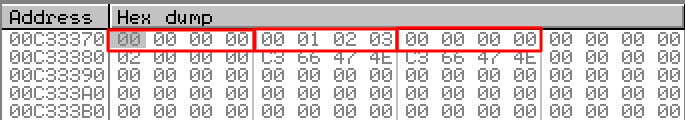
\includegraphics[scale=\NormalScale]{patterns/13_arrays/5_multidimensional/olly_2D_1.png}
\caption{\olly: \RU{массив заполнен}\EN{array is filled}}
\end{figure}

\subsubsection{\RU{Пример с заполнением столбца}\EN{Column filling example}}
\index{\olly}

\RU{Заполняем третий столбец значениями}\EN{Let's fill the third column with values:} 0..2:

\lstinputlisting[caption=\RU{Пример с заполнением столбца}\EN{Column filling example}]{patterns/13_arrays/5_multidimensional/two2.c.\LANG}

\RU{Здесь также обведены красным три строки}\EN{The three rows are also marked in red here}. 
\RU{Видно, что в каждой строке, на третьей позиции, теперь записаны}
\EN{We see that in each row, at third position these values are written:} 0, 1 \AndENRU 2.

\begin{figure}[H]
\centering
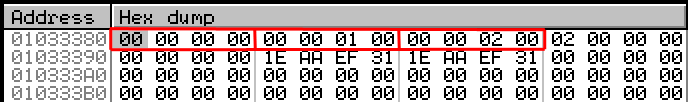
\includegraphics[scale=\NormalScale]{patterns/13_arrays/5_multidimensional/olly_2D_2.png}
\caption{\olly: \RU{массив заполнен}\EN{array is filled}}
\end{figure}

\subsection{\RU{Работа с двухмерным массивом как с одномерным}
\EN{Access two-dimensional array as one-dimensional}}

\RU{Мы можем легко убедиться, что можно работать с двухмерным массивом как с одномерным,
используя по крайней мере два метода:}
\EN{We can be easily assured that it's possible to access a two-dimensional array as one-dimensional array in at least two ways:}

\lstinputlisting{patterns/13_arrays/5_multidimensional/2D_as_1D.c.\LANG}

\RU{Компилируете и запускаете: мы увидим корректные значения.}
\EN{Compile and run it: it shows correct values.}

\RU{Очарователен результат работы MSVC 2013~--- все три процедуры одинаковые!}
\EN{What MSVC 2013 did is fascinating, all three routines are just the same!}

\lstinputlisting[caption=\Optimizing MSVC 2013 x64]{patterns/13_arrays/5_multidimensional/2D_as_1D_MSVC_2013_Ox_x64.asm.\LANG}

\ifdefined\IncludeGCC
\RU{GCC сгенерировал практически одинаковые процедуры:}
\EN{GCC also generates equivalent routines, but slightly different:}

\lstinputlisting[caption=\Optimizing GCC 4.9 x64]{patterns/13_arrays/5_multidimensional/2D_as_1D_GCC49_x64_O3.s.\LANG}
\fi

\subsection{\RU{Пример с трехмерным массивом}\EN{Three-dimensional array example}}

\RU{То же самое и для многомерных массивов.}\EN{It's thing in multidimensional arrays.}
\RU{На этот раз будем работать с массивом типа \Tint: каждый элемент требует 4 байта в памяти.}
\EN{Now we are going to work with an array of type \Tint: each element requires 4 bytes in memory.}

\RU{Попробуем}\EN{Let's see}:

\lstinputlisting[caption=\RU{простой пример}\EN{simple example}]{patterns/13_arrays/5_multidimensional/multi.c}

\subsubsection{x86}

\RU{В итоге}\EN{We get} (MSVC 2010):

\lstinputlisting[caption=MSVC 2010]{patterns/13_arrays/5_multidimensional/multi_msvc.asm.\LANG}

\RU{В принципе, ничего удивительного. В \TT{insert()} для вычисления адреса нужного элемента массива 
три входных аргумента перемножаются по формуле $address=600 \cdot 4 \cdot x + 30 \cdot 4 \cdot y + 4z$, 
чтобы представить массив трехмерным.
Не забывайте также, что тип \Tint 32-битный (4 байта), поэтому все коэффициенты нужно умножить на 4.}
\EN{Nothing special. For index calculation, three input arguments are used 
in the formula $address=600 \cdot 4 \cdot x + 30 \cdot 4 \cdot y + 4z$, to represent the array as multidimensional.
Do not forget that the \Tint type is 32-bit (4 bytes),
so all coefficients must be multiplied by 4.}

\lstinputlisting[caption=GCC 4.4.1]{patterns/13_arrays/5_multidimensional/multi_gcc.asm.\LANG}

\RU{Компилятор GCC решил всё сделать немного иначе}\EN{The GCC compiler does it differently}.
\RU{Для вычисления одной из операций ($30y$), GCC создал код, где нет самой операции умножения.}
\EN{For one of the operations in the calculation ($30y$), GCC produces code without multiplication instructions.}
\RU{Происходит это так}\EN{This is how it done}: 
$(y+y) \ll 4 - (y+y) = (2y) \ll 4 - 2y = 2 \cdot 16 \cdot y - 2y = 32y - 2y = 30y$. 
\RU{Таким образом, для вычисления $30y$ используется только операция сложения, 
операция битового сдвига и операция вычитания.}\EN{Thus, for the $30y$ calculation, only one addition operation,
one bitwise shift operation and one subtraction operation are used.}
\RU{Это работает быстрее}\EN{This works faster}.

\ifdefined\IncludeARM
\subsubsection{ARM + \NonOptimizingXcodeIV (\ThumbMode)}

\lstinputlisting[caption=\NonOptimizingXcodeIV (\ThumbMode)]{patterns/13_arrays/5_multidimensional/multi_Xcode_thumb_O0.asm.\LANG}

\NonOptimizing LLVM \RU{сохраняет все переменные в локальном стеке, хотя это и избыточно.}
\EN{saves all variables in local stack, which is redundant.}
\RU{Адрес элемента массива вычисляется по уже рассмотренной формуле.}
\EN{The address of the array element is calculated by the formula we already saw.}

\subsubsection{ARM + \OptimizingXcodeIV (\ThumbMode)}

\lstinputlisting[caption=\OptimizingXcodeIV (\ThumbMode)]{patterns/13_arrays/5_multidimensional/multi_Xcode_thumb_O3.asm.\LANG}

\RU{Тут используются уже описанные трюки для замены умножения на операции сдвига, сложения и вычитания.}
\EN{The tricks for replacing multiplication by shift, addition and subtraction which we already saw
are also present here.}

\index{ARM!\Instructions!RSB}
\index{ARM!\Instructions!SUB}
\RU{Также мы видим новую для себя инструкцию}\EN{Here we also see a new instruction for us:} 
\RSB (\IT{Reverse Subtract}).
\RU{Она работает так же, как и \SUB, только меняет операнды местами.}
\EN{It works just as \SUB, but it swaps its operands with each other before execution.}
\RU{Зачем?}\EN{Why?}
\index{ARM!Optional operators!LSL}
\SUB \AndENRU \RSB\RU{ это те инструкции, ко второму операнду которых 
можно применить коэффициент сдвига, как мы видим и здесь}%
\EN{ are instructions, to the second operand of which shift coefficient may be applied}: 
(\INS{LSL\#4}). 
\RU{Но этот коэффициент можно применить только ко второму операнду.}
\EN{But this coefficient can be applied only to second operand.}
\RU{Для коммутативных операций, таких как сложение или умножение, 
операнды можно менять местами и это не влияет на результат.}
\EN{That's fine for commutative operations like addition or multiplication 
(operands may be swapped there without changing the result).}
\RU{Но вычитание~--- операция некоммутативная, так что для этих случаев существует инструкция \RSB.}
\EN{But subtraction is a non-commutative operation, so \RSB exist for these cases.}

\index{ARM!\Instructions!LDR.W}
\EN{The}\RU{Инструкция} \INS{LDR.W R9, [R9]} \RU{работает как}\EN{instruction works like} \LEA~(\myref{sec:LEA})
\RU{в x86, и здесь она ничего не делает, она избыточна.}
\EN{in x86, but it does nothing here, it is redundant.}
\RU{Вероятно, компилятор не оптимизировал её.}\EN{Apparently, the compiler did not optimize it out.}
\fi

\ifdefined\IncludeMIPS
\subsubsection{MIPS}

\index{MIPS!Global Pointer}
\EN{My example is tiny, so the GCC compiler decided to put the $a$ array into the 64KiB area 
addressable by the Global Pointer.}
\RU{Мой пример такой крошечный, что компилятор GCC решил разместить массив $a$ в 64KiB-области,
адресуемой при помощи Global Pointer.}

\lstinputlisting[caption=\Optimizing GCC 4.4.5 (IDA)]{patterns/13_arrays/5_multidimensional/multi_MIPS_O3_IDA.lst.\LANG}

\fi


\ifx\LITE\undefined
\subsection{\RU{Ещё примеры}\EN{More examples}}

\RU{Компьютерный экран представляет собой двумерный массив, но видеобуфер это линейный
одномерный массив}\EN{The computer screen is represented as a 2D array, but the video-buffer is 
a linear 1D array}. 
\RU{Мы рассматриваем это здесь}\EN{We talk about it here}: \myref{Mandelbrot_demo}.
\fi

\ifx\LITE\undefined
\section{\RU{Набор строк как двухмерный массив}\EN{Pack of strings as a two-dimensional array}}

\RU{Снова вернемся к примеру, который возвращает название месяца:}%
\EN{Let's revisit the function that returns the name of a month:} \lstref{get_month1}.
\RU{Как видно, нужна как минимум одна операция загрузки из памяти для подготовки указателя на строку,
состоящую из имени месяца.}
\EN{As you see, at least one memory load operation is needed to prepare a pointer to the string
that's the month's name.}
\RU{Возможно ли избавиться от операции загрузки из памяти?}
\EN{Is it possible to get rid of this memory load operation?}
\RU{Да, если представить список строк как двумерный массив:}
\EN{In fact yes, if you represent the list of strings as a two-dimensional array:}

\lstinputlisting{patterns/13_arrays/55_month_2D/month2.c.\LANG}

\RU{Вот что получаем:}\EN{Here is what we've get:}

\lstinputlisting[caption=\Optimizing MSVC 2013 x64]{patterns/13_arrays/55_month_2D/MSVC2013_x64_Ox.asm.\LANG}

\RU{Здесь нет обращений к памяти вообще}\EN{There are no memory accesses at all}.
\RU{Эта функция только вычисляет место, где находится первый символ названия месяца:}
\EN{All this function does is to calculate a point at which the first character of the name of the month is:} 
$pointer\_to\_the\_table + month * 10$.
\RU{Там также две инструкции \LEA, которые работают как несколько инструкций \MUL и \MOV.}
\EN{There are also two \LEA instructions, which effectively work as several \MUL and \MOV instructions.}

\RU{Ширина массива~--- 10 байт}\EN{The width of the array is 10 bytes}. 
\RU{Действительно, самая длинная строка это \q{September} (9 байт) плюс оконечивающий ноль, получается 10 байт.}
\EN{Indeed, the longest string here---\q{September}---is 9 bytes, and plus the terminating zero is 10 bytes.}
\RU{Остальные названия месяцев дополнены нулевыми байтами, чтобы они занимали столько же места (10 байт).}
\EN{The rest of the month names are padded by zero bytes, so they all occupy the same space (10 bytes).}
\RU{Таким образом, наша функция и работает быстрее, потому что все строки начинаются с тех адресов, 
которые легко вычислить.}
\EN{Thus, our function works even faster, because all string start at an address which can be
calculated easily.}

\Optimizing GCC 4.9 \RU{может ещё короче}\EN{can do it even shorter}:

\begin{lstlisting}[caption=\Optimizing GCC 4.9 x64]
	movsx	rdi, edi
	lea	rax, [rdi+rdi*4]
	lea	rax, month2[rax+rax]
	ret
\end{lstlisting}

\RU{\LEA здесь также используется для умножения на 10.}
\EN{\LEA is also used here for multiplication by 10.}

\RU{Неоптимизирующие компиляторы делают умножение по-разному.}
\EN{Non-optimizing compilers do multiplication differently.}

\lstinputlisting[caption=\NonOptimizing GCC 4.9 x64]{patterns/13_arrays/55_month_2D/x64_GCC49_O0.asm.\LANG}

\NonOptimizing MSVC \RU{просто использует инструкцию \IMUL}\EN{just uses \IMUL instruction}:
\index{x86!\Instructions!IMUL}

\lstinputlisting[caption=\NonOptimizing MSVC 2013 x64]{patterns/13_arrays/55_month_2D/MSVC2013_x64.asm.\LANG}

\index{\CompilerAnomaly}
\label{MSVC2013_anomaly}
\RU{Но вот что странно: зачем добавлять умножение на ноль и добавлять ноль к конечному результату?}
\EN{But one thing is weird here: why add multiplication by zero and adding zero to the final result?}
\RU{Это выглядит как странность кодегенератора компилятора, который не был покрыт тестами
компилятора. Но так или иначе, итоговый код работает корректно.}%
\EN{This looks like a compiler code generator quirk, which wasn't caught by the compiler's tests
(the resulting code works correctly, after all).}
% класс!
\RU{Мы сознательно рассматриваем такие фрагменты кода, чтобы читатель понимал, что иногда не нужно
ломать себе голову над подобными артефактами компиляторов.}%
\EN{We intentionally consider such pieces of code so the reader would understand, 
that sometimes one shouldn't puzzle over such compiler artifacts.}

\ifdefined\IncludeARM
\subsection{32-bit ARM}

\Optimizing Keil \RU{для режима Thumb использует инструкцию умножения}
\EN{for Thumb mode uses the multiplication instruction} \INS{MULS}:

\lstinputlisting[caption=\OptimizingKeilVI (\ThumbMode)]{patterns/13_arrays/55_month_2D/Keil_O3_thumb.asm.\LANG}

\Optimizing Keil \RU{для режима ARM использует операции сложения и сдвига}\EN{for ARM mode uses add and 
shift operations}:

\lstinputlisting[caption=\OptimizingKeilVI (\ARMMode)]{patterns/13_arrays/55_month_2D/Keil_O3_ARM.asm.\LANG}

\subsection{ARM64}

\lstinputlisting[caption=\Optimizing GCC 4.9 ARM64]{patterns/13_arrays/55_month_2D/GCC49_ARM64.asm.\LANG}

\index{ARM!\Instructions!SXTW}
\index{ARM!\Instructions!ADRP/ADD pair}
\RU{\INS{SXTW} используется для знакового расширения и расширения
входного 32-битного значения в 64-битное и сохранения его в X0.}
\EN{\INS{SXTW} is used for sign-extension and promoting input 32-bit value into a 64-bit one and storing it in X0.}
\RU{Пара \ADRP/\ADD используется для загрузки адреса таблицы.}
\EN{\ADRP/\ADD pair is used for loading the address of the table.}
\RU{У инструкции \ADD также есть суффикс \LSL, что помогает с умножением.}
\EN{The \ADD instructions also has a \LSL suffix, which helps with multiplications.}
\fi

\ifdefined\IncludeMIPS
\subsection{MIPS}
\lstinputlisting[caption=\Optimizing GCC 4.4.5 (IDA)]{patterns/13_arrays/55_month_2D/MIPS_O3_IDA.lst.\LANG}
\fi

\subsection{\Conclusion{}}

\RU{Это немного старинная техника для хранения текстовых строк.}
\EN{This is a bit old-school technique to store text strings.}
\RU{Много такого можно найти в \oracle, например.}
\EN{You may find a lot of it in \oracle, for example.}
\RU{Трудно сказать, стоит ли оно того на современных компьютерах.}
\EN{It's hard to say if it's worth doing on modern computers.}
\RU{Так или иначе, это был хороший пример массивов, поэтому он был добавлен в эту книгу.}
\EN{Nevertheless, it was a good example of arrays, so it was added to this book.}

\fi
\section{\Conclusion{}}

\RU{Массив это просто набор значений в памяти, расположенных рядом друг с другом.}
\EN{An array is a pack of values in memory located adjacently.}
\RU{Это справедливо для любых типов элементов, включая структуры.}
\EN{It's true for any element type, including structures.}
\RU{Доступ к определенному элементу массива это просто вычисление его адреса.}
\EN{Access to a specific array element is just a calculation of its address.}

\ifdefined\IncludeExercises
\section{\Exercises}

\subsection{\Exercise \#1}
% matrix addition
\label{exercise_array_1}

\WhatThisCodeDoes\

\lstinputlisting[caption=MSVC 2010 + \TT{/O1}]{patterns/13_arrays/exercises/1_msvc.asm}

(/O1: \RU{оптимизация по размеру кода}\EN{minimize space}).

\lstinputlisting[caption=\OptimizingKeilVI (\ARMMode)]{patterns/13_arrays/exercises/1_ARM.s}

\lstinputlisting[caption=\OptimizingKeilVI (\ThumbMode)]{patterns/13_arrays/exercises/1_thumb.s}

\lstinputlisting[caption=\NonOptimizing GCC 4.9 (ARM64)]{patterns/13_arrays/exercises/1_GCC49_ARM64_O0.s}

\lstinputlisting[caption=\Optimizing GCC 4.4.5 (MIPS) (IDA)]{patterns/13_arrays/exercises/1_MIPS_O3_IDA.lst}

\Answer\: \myref{exercise_solutions_arrays_1}.

\subsection{\Exercise \#2}
% matrix multiplication
\label{exercise_array_2}

\WhatThisCodeDoes\

\lstinputlisting[caption=MSVC 2010 + \TT{/O1}]{patterns/13_arrays/exercises/2_msvc.asm}

(/O1: \RU{оптимизация по размеру кода}\EN{minimize space}).

\lstinputlisting[caption=\OptimizingKeilVI (\ARMMode)]{patterns/13_arrays/exercises/2_ARM.s}

\lstinputlisting[caption=\OptimizingKeilVI (\ThumbMode)]{patterns/13_arrays/exercises/2_thumb.s}

\lstinputlisting[caption=\NonOptimizing GCC 4.9 (ARM64)]{patterns/13_arrays/exercises/2_GCC49_ARM64_O0.s}

\lstinputlisting[caption=\Optimizing GCC 4.4.5 (MIPS) (IDA)]{patterns/13_arrays/exercises/2_MIPS_O3_IDA.lst}

\Answer\: \myref{exercise_solutions_arrays_2}.

\subsection{\Exercise \#3}
\label{exercise_array_3}

\WhatThisCodeDoes\

\EN{Try to determine the dimensions of the array, at least partially.}
\RU{Попробуйте определить размеры массива, хотя бы частично.}

\begin{lstlisting}[caption=\Optimizing MSVC 2010]
_array$ = 8
_x$ = 12
_y$ = 16
_f	PROC
	mov	eax, DWORD PTR _x$[esp-4]
	mov	edx, DWORD PTR _y$[esp-4]
	mov	ecx, eax
	shl	ecx, 4
	sub	ecx, eax
	lea	eax, DWORD PTR [edx+ecx*8]
	mov	ecx, DWORD PTR _array$[esp-4]
	fld	QWORD PTR [ecx+eax*8]
	ret	0
_f	ENDP
\end{lstlisting}

\begin{lstlisting}[caption=\NonOptimizingKeilVI (\ARMMode)]
f PROC
        RSB      r1,r1,r1,LSL #4
        ADD      r0,r0,r1,LSL #6
        ADD      r1,r0,r2,LSL #3
        LDM      r1,{r0,r1}
        BX       lr
        ENDP
\end{lstlisting}

\begin{lstlisting}[caption=\NonOptimizingKeilVI (\ThumbMode)]
f PROC
        MOVS     r3,#0xf
        LSLS     r3,r3,#6
        MULS     r1,r3,r1
        ADDS     r0,r1,r0
        LSLS     r1,r2,#3
        ADDS     r1,r0,r1
        LDM      r1,{r0,r1}
        BX       lr
        ENDP
\end{lstlisting}

\begin{lstlisting}[caption=\Optimizing GCC 4.9 (ARM64)]
f:
	sxtw	x1, w1
	add	x0, x0, x2, sxtw 3
	lsl	x2, x1, 10
	sub	x1, x2, x1, lsl 6
	ldr	d0, [x0,x1]
	ret
\end{lstlisting}

\lstinputlisting[caption=\Optimizing GCC 4.4.5 (MIPS) (IDA)]{patterns/13_arrays/exercises/3_MIPS_O3_IDA.lst}

\Answer\: \myref{exercise_solutions_arrays_3}

\subsection{\Exercise \#4}
\label{exercise_array_4}

\WhatThisCodeDoes\

\EN{Try to determine the dimensions of the array, at least partially.}
\RU{Попробуйте определить размеры массива, хотя бы частично.}

\begin{lstlisting}[caption=\Optimizing MSVC 2010]
_array$ = 8	
_x$ = 12	
_y$ = 16	
_z$ = 20	
_f	PROC
	mov	eax, DWORD PTR _x$[esp-4]
	mov	edx, DWORD PTR _y$[esp-4]
	mov	ecx, eax
	shl	ecx, 4
	sub	ecx, eax
	lea	eax, DWORD PTR [edx+ecx*4]
	mov	ecx, DWORD PTR _array$[esp-4]
	lea	eax, DWORD PTR [eax+eax*4]
	shl	eax, 4
	add	eax, DWORD PTR _z$[esp-4]
	mov	eax, DWORD PTR [ecx+eax*4]
	ret	0
_f	ENDP
\end{lstlisting}

\begin{lstlisting}[caption=\NonOptimizingKeilVI (\ARMMode)]
f PROC
        RSB      r1,r1,r1,LSL #4
        ADD      r1,r1,r1,LSL #2
        ADD      r0,r0,r1,LSL #8
        ADD      r1,r2,r2,LSL #2
        ADD      r0,r0,r1,LSL #6
        LDR      r0,[r0,r3,LSL #2]
        BX       lr
        ENDP
\end{lstlisting}

\begin{lstlisting}[caption=\NonOptimizingKeilVI (\ThumbMode)]
f PROC
        PUSH     {r4,lr}
        MOVS     r4,#0x4b
        LSLS     r4,r4,#8
        MULS     r1,r4,r1
        ADDS     r0,r1,r0
        MOVS     r1,#0xff
        ADDS     r1,r1,#0x41
        MULS     r2,r1,r2
        ADDS     r0,r0,r2
        LSLS     r1,r3,#2
        LDR      r0,[r0,r1]
        POP      {r4,pc}
        ENDP
\end{lstlisting}

\begin{lstlisting}[caption=\Optimizing GCC 4.9 (ARM64)]
f:
	sxtw	x2, w2
	mov	w4, 19200
	add	x2, x2, x2, lsl 2
	smull	x1, w1, w4
	lsl	x2, x2, 4
	add	x3, x2, x3, sxtw
	add	x0, x0, x3, lsl 2
	ldr	w0, [x0,x1]
	ret
\end{lstlisting}

\lstinputlisting[caption=\Optimizing GCC 4.4.5 (MIPS) (IDA)]{patterns/13_arrays/exercises/4_MIPS_O3_IDA.lst}

\Answer\: \myref{exercise_solutions_arrays_4}

\subsection{\Exercise \#5}
\label{exercise_array_5}

\WhatThisCodeDoes\

\begin{lstlisting}[caption=\Optimizing MSVC 2012 /GS-]
COMM	_tbl:DWORD:064H

tv759 = -4	; size = 4
_main	PROC
	push	ecx
	push	ebx
	push	ebp
	push	esi
	xor	edx, edx
	push	edi
	xor	esi, esi
	xor	edi, edi
	xor	ebx, ebx
	xor	ebp, ebp
	mov	DWORD PTR tv759[esp+20], edx
	mov	eax, OFFSET _tbl+4
	npad	8 ; align next label
$LL6@main:
	lea	ecx, DWORD PTR [edx+edx]
	mov	DWORD PTR [eax+4], ecx
	mov	ecx, DWORD PTR tv759[esp+20]
	add	DWORD PTR tv759[esp+20], 3
	mov	DWORD PTR [eax+8], ecx
	lea	ecx, DWORD PTR [edx*4]
	mov	DWORD PTR [eax+12], ecx
	lea	ecx, DWORD PTR [edx*8]
	mov	DWORD PTR [eax], edx
	mov	DWORD PTR [eax+16], ebp
	mov	DWORD PTR [eax+20], ebx
	mov	DWORD PTR [eax+24], edi
	mov	DWORD PTR [eax+32], esi
	mov	DWORD PTR [eax-4], 0
	mov	DWORD PTR [eax+28], ecx
	add	eax, 40
	inc	edx
	add	ebp, 5
	add	ebx, 6
	add	edi, 7
	add	esi, 9
	cmp	eax, OFFSET _tbl+404
	jl	SHORT $LL6@main
	pop	edi
	pop	esi
	pop	ebp
	xor	eax, eax
	pop	ebx
	pop	ecx
	ret	0
_main	ENDP
\end{lstlisting}

\begin{lstlisting}[caption=\NonOptimizingKeilVI (\ARMMode)]
main PROC
        LDR      r12,|L0.60|
        MOV      r1,#0
|L0.8|
        ADD      r2,r1,r1,LSL #2
        MOV      r0,#0
        ADD      r2,r12,r2,LSL #3
|L0.20|
        MUL      r3,r1,r0
        STR      r3,[r2,r0,LSL #2]
        ADD      r0,r0,#1
        CMP      r0,#0xa
        BLT      |L0.20|
        ADD      r1,r1,#1
        CMP      r1,#0xa
        MOVGE    r0,#0
        BLT      |L0.8|
        BX       lr
        ENDP

|L0.60|
        DCD      ||.bss||

        AREA ||.bss||, DATA, NOINIT, ALIGN=2

tbl
        %        400
\end{lstlisting}

\begin{lstlisting}[caption=\NonOptimizingKeilVI (\ThumbMode)]
main PROC
        PUSH     {r4,r5,lr}
        LDR      r4,|L0.40|
        MOVS     r1,#0
|L0.6|
        MOVS     r2,#0x28
        MULS     r2,r1,r2
        MOVS     r0,#0
        ADDS     r3,r2,r4
|L0.14|
        MOVS     r2,r1
        MULS     r2,r0,r2
        LSLS     r5,r0,#2
        ADDS     r0,r0,#1
        CMP      r0,#0xa
        STR      r2,[r3,r5]
        BLT      |L0.14|
        ADDS     r1,r1,#1
        CMP      r1,#0xa
        BLT      |L0.6|
        MOVS     r0,#0
        POP      {r4,r5,pc}
        ENDP

        DCW      0x0000
|L0.40|
        DCD      ||.bss||

        AREA ||.bss||, DATA, NOINIT, ALIGN=2

tbl
        %        400
\end{lstlisting}

\begin{lstlisting}[caption=\NonOptimizing GCC 4.9 (ARM64)]
	.comm	tbl,400,8
main:
	sub	sp, sp, #16
	str	wzr, [sp,12]
	b	.L2
.L5:
	str	wzr, [sp,8]
	b	.L3
.L4:
	ldr	w1, [sp,12]
	ldr	w0, [sp,8]
	mul	w3, w1, w0
	adrp	x0, tbl
	add	x2, x0, :lo12:tbl
	ldrsw	x4, [sp,8]
	ldrsw	x1, [sp,12]
	mov	x0, x1
	lsl	x0, x0, 2
	add	x0, x0, x1
	lsl	x0, x0, 1
	add	x0, x0, x4
	str	w3, [x2,x0,lsl 2]
	ldr	w0, [sp,8]
	add	w0, w0, 1
	str	w0, [sp,8]
.L3:
	ldr	w0, [sp,8]
	cmp	w0, 9
	ble	.L4
	ldr	w0, [sp,12]
	add	w0, w0, 1
	str	w0, [sp,12]
.L2:
	ldr	w0, [sp,12]
	cmp	w0, 9
	ble	.L5
	mov	w0, 0
	add	sp, sp, 16
	ret
\end{lstlisting}

\lstinputlisting[caption=\NonOptimizing GCC 4.4.5 (MIPS) (IDA)]{patterns/13_arrays/exercises/5_MIPS_O0_IDA.lst}

\Answer\: \myref{exercise_solutions_arrays_5}

\fi

\chapter{\BitfieldsChapter}
\label{sec:bitfields}

\RU{Немало функций задают различные флаги в аргументах при помощи битовых 
полей\footnote{bit fields в англоязычной литературе}.}
\EN{A lot of functions define their input arguments as flags in bit fields.}
\index{\CLanguageElements!C99!bool}
\RU{Наверное, вместо этого можно было бы использовать набор переменных типа \Tbool, но это было бы 
не очень экономно.}
\EN{Of course, they could be substituted by a set of \Tbool-typed variables, but it is not frugally.}

% sections
\section{\RU{Проверка какого-либо бита}\EN{Specific bit checking}}

\subsection{x86}
\index{Windows!Win32}

\RU{Например в Win32 API:}\EN{Win32 API example:}

\begin{lstlisting}
	HANDLE fh;

	fh=CreateFile ("file", GENERIC_WRITE | GENERIC_READ, FILE_SHARE_READ, NULL, OPEN_ALWAYS, FILE_ATTRIBUTE_NORMAL, NULL);
\end{lstlisting}

\RU{Получаем}\EN{We get} (MSVC 2010):

\begin{lstlisting}[caption=MSVC 2010]
	push	0
	push	128					; 00000080H
	push	4
	push	0
	push	1
	push	-1073741824				; c0000000H
	push	OFFSET $SG78813
	call	DWORD PTR __imp__CreateFileA@28
	mov	DWORD PTR _fh$[ebp], eax
\end{lstlisting}

\RU{Заглянем в файл}\EN{Let's take a look in} WinNT.h:

\begin{lstlisting}[caption=WinNT.h]
#define GENERIC_READ                     (0x80000000L)
#define GENERIC_WRITE                    (0x40000000L)
#define GENERIC_EXECUTE                  (0x20000000L)
#define GENERIC_ALL                      (0x10000000L)
\end{lstlisting}

\RU{Всё ясно}\EN{Everything is clear}, 
\TT{GENERIC\_READ | GENERIC\_WRITE = 0x80000000 | 0x40000000 = 0xC0000000}, 
\RU{и это значение используется как второй аргумент для функции}
\EN{and that value is used as the second argument for the} \TT{CreateFile()}\footnote{\href{http://go.yurichev.com/17065}{msdn.microsoft.com/en-us/library/aa363858(VS.85).aspx}}\EN{function}.

\RU{Как \TT{CreateFile()} будет проверять флаги?}\EN{How would \TT{CreateFile()} check these flags?}
\index{Windows!KERNEL32.DLL}
\RU{Заглянем в KERNEL32.DLL от Windows XP SP3 x86 и найдем в функции \TT{CreateFileW()} в том числе и 
такой фрагмент кода:}
\EN{If we look in KERNEL32.DLL in Windows XP SP3 x86, we'll find
this fragment of code in \TT{CreateFileW}:}

\begin{lstlisting}[caption=KERNEL32.DLL (Windows XP SP3 x86)]
.text:7C83D429                 test    byte ptr [ebp+dwDesiredAccess+3], 40h
.text:7C83D42D                 mov     [ebp+var_8], 1
.text:7C83D434                 jz      short loc_7C83D417
.text:7C83D436                 jmp     loc_7C810817
\end{lstlisting}

\index{x86!\Instructions!TEST}
\RU{Здесь мы видим инструкцию \TEST. Впрочем, она берет не весь второй аргумент функции, 
а только его самый старший байт (\TT{ebp+dwDesiredAccess+3}) и проверяет его на флаг \TT{0x40}
(имеется ввиду флаг \TT{GENERIC\_WRITE}).}
\EN{Here we see the \TEST instruction, however it doesn't take the whole second argument,
but only the most significant byte (\TT{ebp+dwDesiredAccess+3}) and checks it for flag \TT{0x40}
(which implies the \TT{GENERIC\_WRITE} flag here)}
\index{x86!\Instructions!AND}
\RU{\TEST это то же что и \AND, только без сохранения результата 
(вспомните что \CMP это то же что и \SUB, только без сохранения результатов}
\EN{\TEST is basically the same instruction as \AND, but without saving the result
(recall the fact \CMP is merely the same as \SUB, but without saving the result}~(\myref{CMPandSUB})).

\RU{Логика данного фрагмента кода примерно такая:}\EN{The logic of this code fragment is as follows:}

\begin{lstlisting}
if ((dwDesiredAccess&0x40000000) == 0) goto loc_7C83D417
\end{lstlisting}

\index{x86!\Instructions!AND}
\index{x86!\Registers!ZF}
\RU{Если после операции \AND останется этот бит, то флаг \ZF не будет поднят и условный переход 
\JZ не сработает. 
Переход возможен, только если в переменной \TT{dwDesiredAccess} отсутствует бит \TT{0x40000000}~--- 
тогда результат \AND будет 0, флаг \ZF будет поднят и переход сработает.}
\EN{If \AND instruction leaves this bit, the \ZF flag is to be cleared and the 
\JZ conditional jump is not to be triggered.
The conditional jump is triggered only if the \TT{0x40000000} bit is absent in \TT{dwDesiredAccess} variable
~---then the result of \AND is 0, \ZF is to be set and the conditional jump is to be triggered.}

\ifdefined\IncludeGCC
\RU{Попробуем GCC 4.4.1 и Linux:}\EN{Let's try GCC 4.4.1 and Linux:}

\begin{lstlisting}
#include <stdio.h>
#include <fcntl.h>

void main()
{
	int handle;

	handle=open ("file", O_RDWR | O_CREAT);
};
\end{lstlisting}

\RU{Получим}\EN{We get}:

\lstinputlisting[caption=GCC 4.4.1]{patterns/14_bitfields/1_check/check.asm}

\index{Linux!libc.so.6}
\index{syscall}
\RU{Заглянем в реализацию функции \TT{open()} в библиотеке \TT{libc.so.6}, но обнаружим что там 
только системный вызов:}
\EN{If we take a look in the \TT{open()} function in the \TT{libc.so.6} library, it is only a syscall:}

\begin{lstlisting}[caption=open() (libc.so.6)]
.text:000BE69B                 mov     edx, [esp+4+mode] ; mode
.text:000BE69F                 mov     ecx, [esp+4+flags] ; flags
.text:000BE6A3                 mov     ebx, [esp+4+filename] ; filename
.text:000BE6A7                 mov     eax, 5
.text:000BE6AC                 int     80h             ; LINUX - sys_open
\end{lstlisting}

\RU{Значит, битовые поля флагов \TT{open()} проверяются где-то в ядре Linux.}
\EN{So, the bit fields for \TT{open()} are apparently checked somewhere in the Linux kernel.}

\RU{Разумеется, и стандартные библиотеки Linux и ядро Linux можно получить в виде исходников, 
но нам интересно попробовать разобраться без них.}
\EN{Of course, it is easy to download both Glibc and the Linux kernel source code, 
but we are interested in understanding the matter without it.}

\RU{При системном вызове \TT{sys\_open} управление в конечном итоге передается в \TT{do\_sys\_open} в ядре Linux 2.6. 
Оттуда~--- в \TT{do\_filp\_open()} (эта функция находится в исходниках ядра в файле \TT{fs/namei.c}).}
\EN{So, as of Linux 2.6, when the \TT{sys\_open} syscall is called, control eventually passes to \TT{do\_sys\_open},
and from there---to the \TT{do\_filp\_open()} function (it's located in the kernel source tree in \TT{fs/namei.c}).}

\newcommand{\URLREGPARM}{\href{http://go.yurichev.com/17040}{ohse.de/uwe/articles/gcc-attributes.html\#func-regparm}}

\index{fastcall}
\label{regparm}
N.B. \RU{Помимо передачи параметров функции через стек, существует также возможность передавать 
некоторые из них через регистры. Такое соглашение о вызове называется fastcall~(\myref{fastcall}).
Оно работает немного быстрее, так как для чтения аргументов процессору не нужно обращаться к стеку, лежащему в памяти. 
В GCC есть опция \IT{regparm}\footnote{\URLREGPARM}, 
и с её помощью можно задать, сколько аргументов можно передать через регистры.}
\EN{Aside from passing arguments via the stack,
there is also a method of passing some of them
via registers. This is also called fastcall~(\myref{fastcall}).
This works faster since CPU does not need to access the stack in memory to read argument values.
GCC has the option \IT{regparm}\footnote{\URLREGPARM},
through which it's possible to set the number of arguments that can be passed via registers.}

\newcommand{\URLKERNELNEWB}{\href{http://go.yurichev.com/17066}{kernelnewbies.org/Linux\_2\_6\_20\#head-042c62f290834eb1fe0a1942bbf5bb9a4accbc8f}}
\newcommand{\CALLINGHFILE}{arch/x86/include/asm/calling.h}

\RU{Ядро Linux 2.6 собирается с опцией \TT{-mregparm=3}\footnote{\URLKERNELNEWB}
\footnote{См. также файл \TT{\CALLINGHFILE} в исходниках ядра}.}
\EN{The Linux 2.6 kernel is compiled with \TT{-mregparm=3} option~\footnote{\URLKERNELNEWB}
\footnote{See also \TT{\CALLINGHFILE} file in kernel tree}.}

\RU{Для нас это означает, что первые три аргумента функции будут передаваться через регистры \EAX, 
\EDX и \ECX, 
а остальные через стек. Разумеется, если аргументов у функции меньше трех, то будет задействована 
только часть этих регистров.}
\EN{What this means to us is that the first 3 arguments are to be passed via registers \EAX, \EDX and \ECX, 
and the rest via the stack. 
Of course, if the number of arguments is less than 3, only part of registers set is to be used.}

\RU{Итак, качаем ядро 2.6.31, собираем его в Ubuntu, открываем в \IDA, 
находим функцию \TT{do\_filp\_open()}. В начале мы увидим что-то такое (комментарии мои):}
\EN{So, let's download Linux Kernel 2.6.31, compile it in Ubuntu: \TT{make vmlinux}, open it in \IDA, 
and find the \TT{do\_filp\_open()} function. At the beginning, we see (the comments are mine):}

\lstinputlisting[caption=do\_filp\_open() (linux kernel 2.6.31)]{patterns/14_bitfields/1_check/check2.asm.\LANG}

\RU{GCC сохраняет значения первых трех аргументов в локальном стеке. Иначе, если эти три регистра 
не трогать вообще, то функции компилятора, распределяющей переменные по регистрам (так называемый 
\gls{register allocator}), 
будет очень тесно.}
\EN{GCC saves the values of the first 3 arguments in the local stack. 
If that wasn't done, the compiler would not touch these registers, 
and that would be too tight environment for the compiler's \gls{register allocator}.}

\RU{Далее находим примерно такой фрагмент кода}\EN{Let's find this fragment of code}:

\lstinputlisting[caption=do\_filp\_open() (linux kernel 2.6.31)]{patterns/14_bitfields/1_check/check3.asm}

\RU{\TT{0x40}~--- это значение макроса \TT{O\_CREAT}. 
\TT{open\_flag} проверяется на наличие бита \TT{0x40} и если бит равен 1, то выполняется следующие 
за \JNZ инструкции.}
\EN{\TT{0x40}---is what the \TT{O\_CREAT} macro equals to.
\TT{open\_flag} gets checked for the presence of the \TT{0x40} bit, and if this bit is 1, 
the next \JNZ instruction is triggered.}
\fi

\ifdefined\IncludeARM
\subsection{ARM}

\index{Linux}
\RU{В ядре Linux 3.8.0 бит \TT{O\_CREAT} проверяется немного иначе.}
\EN{The \TT{O\_CREAT} bit is checked differently in Linux kernel 3.8.0.}

\begin{lstlisting}[caption=linux kernel 3.8.0]
struct file *do_filp_open(int dfd, struct filename *pathname,
		const struct open_flags *op)
{
...
	filp = path_openat(dfd, pathname, &nd, op, flags | LOOKUP_RCU);
...
}

static struct file *path_openat(int dfd, struct filename *pathname,
		struct nameidata *nd, const struct open_flags *op, int flags)
{
...
	error = do_last(nd, &path, file, op, &opened, pathname);
...
}


static int do_last(struct nameidata *nd, struct path *path,
		   struct file *file, const struct open_flags *op,
		   int *opened, struct filename *name)
{
...
	if (!(open_flag & O_CREAT)) {
    ...
		error = lookup_fast(nd, path, &inode);
    ...
	} else {
    ...
		error = complete_walk(nd);
        }
...
}
\end{lstlisting}

\RU{Вот как это выглядит в \IDA, ядро скомпилированное для режима ARM:}
\EN{Here is how the kernel compiled for ARM mode looks in \IDA:}

\begin{lstlisting}[caption=do\_last() (vmlinux)]
...
.text:C0169EA8                 MOV             R9, R3  ; R3 - (4th argument) open_flag
...
.text:C0169ED4                 LDR             R6, [R9] ; R6 - open_flag
...
.text:C0169F68                 TST             R6, #0x40 ; jumptable C0169F00 default case
.text:C0169F6C                 BNE             loc_C016A128
.text:C0169F70                 LDR             R2, [R4,#0x10]
.text:C0169F74                 ADD             R12, R4, #8
.text:C0169F78                 LDR             R3, [R4,#0xC]
.text:C0169F7C                 MOV             R0, R4
.text:C0169F80                 STR             R12, [R11,#var_50]
.text:C0169F84                 LDRB            R3, [R2,R3]
.text:C0169F88                 MOV             R2, R8
.text:C0169F8C                 CMP             R3, #0
.text:C0169F90                 ORRNE           R1, R1, #3
.text:C0169F94                 STRNE           R1, [R4,#0x24]
.text:C0169F98                 ANDS            R3, R6, #0x200000
.text:C0169F9C                 MOV             R1, R12
.text:C0169FA0                 LDRNE           R3, [R4,#0x24]
.text:C0169FA4                 ANDNE           R3, R3, #1
.text:C0169FA8                 EORNE           R3, R3, #1
.text:C0169FAC                 STR             R3, [R11,#var_54]
.text:C0169FB0                 SUB             R3, R11, #-var_38
.text:C0169FB4                 BL              lookup_fast
...
.text:C016A128 loc_C016A128                            ; CODE XREF: do_last.isra.14+DC
.text:C016A128                 MOV             R0, R4
.text:C016A12C                 BL              complete_walk
...
\end{lstlisting}

\index{ARM!\Instructions!TST}
\index{x86!\Instructions!TEST}
\TT{TST} \RU{это аналог инструкции \TEST в x86.}\EN{is analogous to the \TEST instruction in x86.}

\RU{Мы можем \q{узнать} визуально этот фрагмент кода по тому что в одном случае исполнится 
функция \TT{lookup\_fast()}, а в другом \TT{complete\_walk()}.}
\EN{We can \q{spot} visually this code fragment by the fact the 
\TT{lookup\_fast()} is to be executed
in one case and \TT{complete\_walk()} in the other.}
\RU{Это соответствует исходному коду функции \TT{do\_last()}.}
\EN{This corresponds to the source code of the \TT{do\_last()} function.}

\EN{The}\RU{Макрос} \TT{O\_CREAT} \RU{здесь так же равен \TT{0x40}.}\EN{macro equals to \TT{0x40} here too.}


\fi


\section{\RU{Установка и сброс отдельного бита}\EN{Setting and clearing specific bits}}

\RU{Например}\EN{For example}:

\lstinputlisting{patterns/14_bitfields/2_set_reset/set_reset.c}
\subsection{x86}

\subsubsection{\NonOptimizing MSVC}

\RU{Имеем в итоге}\EN{We get} (MSVC 2010):

\lstinputlisting[caption=MSVC 2010]{patterns/14_bitfields/2_set_reset/set_reset_msvc.asm}

\index{x86!\Instructions!OR}
\RU{Инструкция \OR здесь устанавливает в переменной ещё один бит, игнорируя остальные.}
\EN{The \OR instruction sets one bit to value while ignoring the rest.}

\index{x86!\Instructions!AND}
\RU{А \AND сбрасывает некий бит. Можно также сказать, что \AND здесь копирует все биты, кроме одного. 
Действительно, во втором операнде \AND выставлены в единицу те биты, которые нужно сохранить, 
кроме одного, копировать который мы не хотим (и который 0 в битовой маске).
Так проще понять и запомнить.}
\EN{\AND resets one bit. It can be said that \AND just copies all bits except one.
Indeed, in the second \AND operand only the bits that need to be saved are set,
just the one do not want to copy is not (which is 0 in the bitmask).
It is the easier way to memorize the logic.}

\ifdefined\IncludeOlly
\clearpage
\myparagraph{\olly}

\RU{Попробуем этот пример в}\EN{Let's try this example in} \olly.
\RU{Сначала, посмотрим на двоичное представление используемых нами констант}
\EN{First, let's see the binary form of the constants we are going to use}:

\TT{0x200} (0000000000000000000{\color{red}1}000000000) 
(\RU{т.е. 10-й бит (считая с первого)}\EN{i.e., the 10th bit (counting from 1st)}).

\RU{Инвертированное}\EN{Inverted} \TT{0x200} \RU{это}\EN{is} \TT{0xFFFFFDFF} 
(1111111111111111111{\color{red}0}111111111).

\TT{0x4000} (00000000000000{\color{red}1}00000000000000) (\RU{т.е. 15-й бит}\EN{i.e., the 15th bit}).

\RU{Входное значение это}\EN{The input value is}: \TT{0x12340678} (10010001101000000011001111000).
\RU{Видим, как оно загрузилось}\EN{We see how it's loaded}:

\begin{figure}[H]
\centering
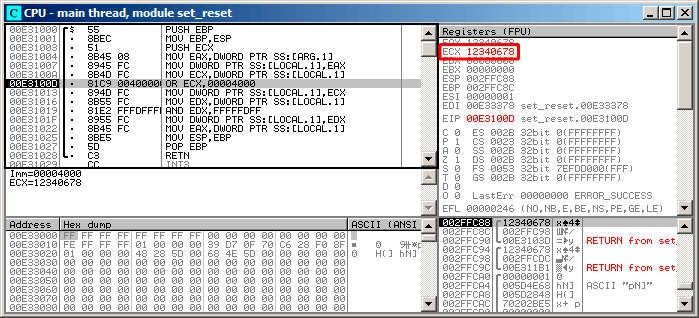
\includegraphics[scale=\FigScale]{patterns/14_bitfields/2_set_reset/olly1.png}
\caption{\olly: \EN{value is loaded into}\RU{значение загружено в} \ECX}
\label{fig:set_reset_olly1}
\end{figure}

\clearpage
\OR \RU{исполнилась}\EN{got executed}:

\begin{figure}[H]
\centering
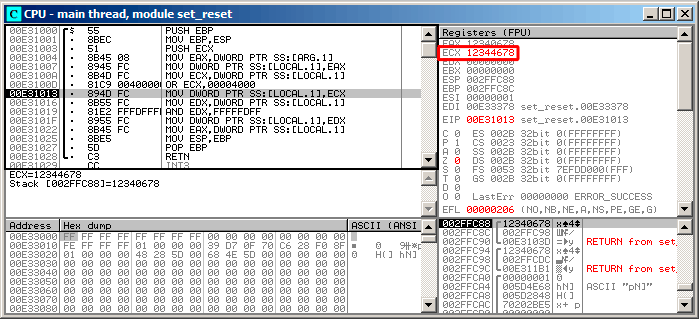
\includegraphics[scale=\FigScale]{patterns/14_bitfields/2_set_reset/olly2.png}
\caption{\olly: \OR \RU{сработал}\EN{executed}}
\label{fig:set_reset_olly2}
\end{figure}

\RU{15-й бит выставлен}\EN{15th bit is set}: \TT{0x1234{\color{red}4}678} 
(10010001101000{\color{red}1}00011001111000).

\clearpage
\RU{Значение перезагружается снова (потому что использовался режим компилятора без оптимизации)}\EN{The value is 
reloaded again (because the compiler is not in optimizing mode)}: 

\begin{figure}[H]
\centering
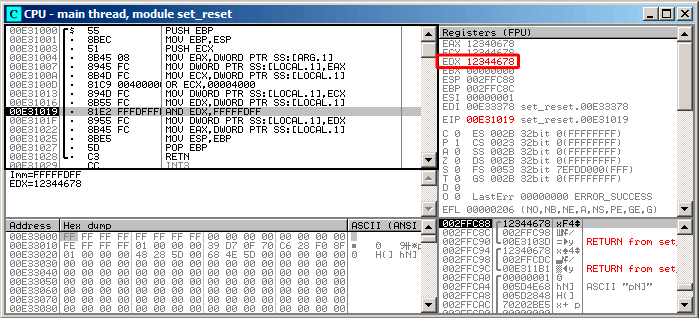
\includegraphics[scale=\FigScale]{patterns/14_bitfields/2_set_reset/olly3.png}
\caption{\olly: \EN{value was reloaded into}\RU{значение перезагрузилось в} \EDX}
\label{fig:set_reset_olly3}
\end{figure}

\clearpage
\AND \RU{исполнилась}\EN{got executed}:

\begin{figure}[H]
\centering
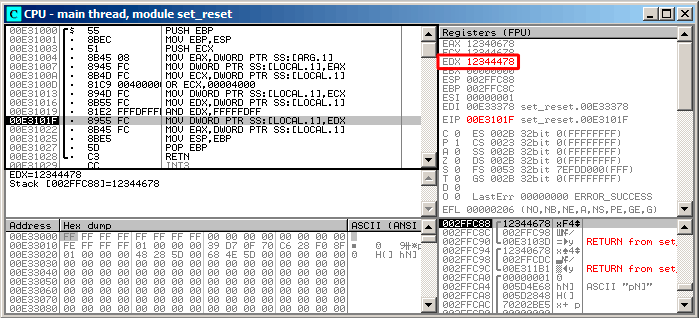
\includegraphics[scale=\FigScale]{patterns/14_bitfields/2_set_reset/olly4.png}
\caption{\olly: \AND \RU{сработал}\EN{executed}}
\label{fig:set_reset_olly4}
\end{figure}

\RU{10-й бит очищен (или, иным языком, оставлены все биты кроме 10-го) и итоговое значение это}
\EN{The 10th bit was cleared (or, in other words, all bits were left except the 10th) and the final value now is}\ESph{}\PTBRph{}\PLph{} \\
\TT{0x12344{\color{red}4}78} (1001000110100010001{\color{red}0}001111000).

\fi

\subsubsection{\Optimizing MSVC}

\RU{Если скомпилировать в MSVC с оптимизацией (\Ox), то код еще короче:}
\EN{If we compile it in MSVC with optimization turned on (\Ox), the code is even shorter:}

\lstinputlisting[caption=\Optimizing MSVC]{patterns/14_bitfields/2_set_reset/set_reset_msvc_Ox.asm}

\ifdefined\IncludeGCC
\subsubsection{\NonOptimizing GCC}

\RU{Попробуем GCC 4.4.1 без оптимизации:}\EN{Let's try GCC 4.4.1 without optimization:}

\lstinputlisting[caption=\NonOptimizing GCC]{patterns/14_bitfields/2_set_reset/set_reset_gcc.asm}

\RU{Также избыточный код, хотя короче, чем у MSVC без оптимизации.}
\EN{There is a redundant code present,
however, it is shorter than the MSVC version without optimization.}

\RU{Попробуем теперь GCC с оптимизацией}\EN{Now let's try GCC with optimization turned on} \Othree:

\subsubsection{\Optimizing GCC}

\lstinputlisting[caption=\Optimizing GCC]{patterns/14_bitfields/2_set_reset/set_reset_gcc_O3.asm}

\RU{Уже короче. Важно отметить, что через регистр \AH компилятор работает с частью регистра \EAX. 
Это его часть от 8-го до 15-го бита включительно.}
\EN{That's shorter.
It is worth noting the compiler works with the \EAX register part via the \AH 
register---that is the \EAX register part from the 8th to the 15th bits included.}

\RegTableOne{RAX}{EAX}{AX}{AH}{AL}

\index{Intel!8086}
\index{Intel!80386}
N.B. \RU{В 16-битном процессоре 8086 аккумулятор имел название \AX 
и состоял из двух 8-битных половин~--- \AL (младшая часть) и \AH (старшая). 
В 80386 регистры были расширены до 32-бит, 
аккумулятор стал называться \EAX, но в целях совместимости, к его \IT{более старым} частям всё ещё можно 
обращаться как к \AX/\AH/\AL.}
\EN{The 16-bit CPU 8086 accumulator was named \AX and consisted of two 8-bit 
halves---\AL (lower byte) and \AH (higher byte).
In 80386 almost all registers were extended to 32-bit, the accumulator was named \EAX, 
but for the sake of compatibility,
its \IT{older parts} may be still accessed as \AX/\AH/\AL.}

\RU{Из-за того, что все x86 процессоры~--- наследники 16-битного 8086, эти \IT{старые} 16-битные опкоды короче 
нежели более новые 32-битные. 
Поэтому инструкция \INS{or ah, 40h} занимает только 3 байта. 
Было бы логичнее сгенерировать здесь \INS{or eax, 04000h}, но это уже 5 байт, или даже 6 
(если регистр в первом операнде не \EAX).}
\EN{Since all x86 CPUs are successors of the 16-bit 8086 CPU, these \IT{older} 16-bit opcodes are shorter 
than the newer 32-bit ones.
That's why the \INS{or ah, 40h} instruction occupies only 3 bytes.
It would be more logical way to emit here \INS{or eax, 04000h}
but that is 5 bytes, or even 6
(in case the register in the first operand is not \EAX).}

\subsubsection{\Optimizing GCC \AndENRU regparm}

\RU{Если мы скомпилируем этот же пример не только с включенной оптимизацией \Othree, 
но ещё и с опцией \TT{regparm=3}, о которой я писал немного выше, то получится ещё короче:}
\EN{It would be even shorter if to turn on the \Othree optimization flag and also set \TT{regparm=3}.}

\lstinputlisting[caption=\Optimizing GCC]{patterns/14_bitfields/2_set_reset/set_reset_gcc_O3_regparm3.asm}

\index{Inline code}
\RU{Действительно~--- первый аргумент уже загружен в \EAX, и прямо здесь можно начинать с ним работать. 
Интересно, что и пролог функции (\INS{push ebp / mov ebp,esp}) и эпилог (\INS{pop ebp}) 
функции можно смело выкинуть за ненадобностью, 
но возможно GCC ещё не так хорош для подобных оптимизаций по размеру кода. 
Впрочем, в реальной жизни подобные короткие функции лучше всего автоматически делать в виде 
\IT{inline-функций} (\myref{inline_code}).}
\EN{Indeed, the first argument is already loaded in \EAX, so it is possible to work with it in-place.
It is worth noting that both the function prologue (\INS{push ebp / mov ebp,esp}) and epilogue (\INS{pop ebp})
can easily be omitted
here, but GCC probably is not good enough to do such code size optimizations.
However, such short functions are better to be \IT{inlined functions} (\myref{inline_code}).}
\fi

\ifdefined\IncludeARM
\subsection{ARM + \OptimizingKeilVI (\ARMMode)}

\begin{lstlisting}[caption=\OptimizingKeilVI (\ARMMode)]
02 0C C0 E3          BIC     R0, R0, #0x200
01 09 80 E3          ORR     R0, R0, #0x4000
1E FF 2F E1          BX      LR
\end{lstlisting}

\index{ARM!\Instructions!BIC}
\INS{BIC} (\IT{BItwise bit Clear}) \RU{это инструкция сбрасывающая заданные биты. 
Это как аналог \AND, но только с инвертированным операндом.}\EN{is an instruction for clearing 
specific bits. This is just like the \AND instruction, but with inverted operand.}
\EN{I.e., it's analogous to a \NOT+\AND instruction pair.}
\RU{Т.е. это аналог инструкций \NOT+\AND.}

\index{ARM!\Instructions!ORR}
\INS{ORR} \RU{это \q{логическое или}, аналог}\EN{is \q{logical or}, analogous to} \OR \InENRU x86.

\RU{Пока всё понятно}\EN{So far it's easy}.

\subsection{ARM + \OptimizingKeilVI (\ThumbMode)}

\begin{lstlisting}[caption=\OptimizingKeilVI (\ThumbMode)]
01 21 89 03          MOVS    R1, 0x4000
08 43                ORRS    R0, R1
49 11                ASRS    R1, R1, #5   ; generate 0x200 and place to R1
88 43                BICS    R0, R1
70 47                BX      LR
\end{lstlisting}

\RU{Вероятно, Keil решил, что код в режиме Thumb,}
\EN{Seems like Keil decided that the code in Thumb mode,}
\RU{получающий}\EN{making} \TT{0x200} \RU{из}\EN{from} \TT{0x4000}, 
\RU{более компактный, нежели код,}\EN{is more compact than the code} 
\RU{записывающий}\EN{for writing} \TT{0x200} \RU{в какой-нибудь регистр}\EN{to an arbitrary register}.
% TODO1 пример, как компилятор при помощи сдвигов оптизирует такое: a=0x1000; b=0x2000; c=0x4000, etc

\index{ARM!\Instructions!ASRS}
\RU{Поэтому при помощи инструкции}
\EN{So that is why, with the help of} \INS{ASRS} 
(\ASRdesc), \RU{это значение вычисляется как}\EN{this value is calculated as} $\TT{0x4000} \gg 5$.

\subsection{ARM + \OptimizingXcodeIV (\ARMMode)}
\label{anomaly:LLVM}
\index{\CompilerAnomaly}

\begin{lstlisting}[caption=\OptimizingXcodeIV (\ARMMode),label=ARM_leaf_example3]
42 0C C0 E3          BIC             R0, R0, #0x4200
01 09 80 E3          ORR             R0, R0, #0x4000
1E FF 2F E1          BX              LR
\end{lstlisting}

\RU{Код, который был сгенерирован LLVM, в исходном коде, на самом деле, выглядел бы так:}
\EN{The code that was generated by LLVM, in source code form could be something like this:}

\begin{lstlisting}
    REMOVE_BIT (rt, 0x4200);
    SET_BIT (rt, 0x4000);
\end{lstlisting}

\RU{И он делает в точности что нам нужно}\EN{And it does exactly what we need}. 
\RU{Но почему}\EN{But why} \TT{0x4200}? 
\RU{Возможно, это артефакт оптимизатора LLVM}%
\EN{Perhaps, that an artifact from LLVM's optimizer}%
\footnote{\RU{Это был}\EN{It was} LLVM build 2410.2.00 \RU{входящий в состав}\EN{bundled with} Apple Xcode 4.6.3}.
\RU{Возможно, ошибка оптимизатора компилятора, но создаваемый код всё же работает верно.}
\EN{Probably a compiler's optimizer error, but the generated code works correctly anyway.}

\RU{Об аномалиях компиляторов, подробнее читайте здесь}
\EN{You can read more about compiler anomalies here}~(\myref{anomaly:Intel}).

\OptimizingXcodeIV \RU{для режима Thumb генерирует точно такой же код.}
\EN{for Thumb mode generates the same code.}

\subsection{ARM: \RU{ещё об инструкции \INS{BIC}}\EN{more about the \INS{BIC} instruction}}
\index{ARM!\Instructions!BIC}

\RU{Если немного переделать пример}\EN{Let's rework the example slightly}:

\begin{lstlisting}
int f(int a)
{
    int rt=a;

    REMOVE_BIT (rt, 0x1234);

    return rt;
};
\end{lstlisting}

\EN{Then the optimizing}\RU{То оптимизирующий} Keil 5.03 
\RU{в режиме ARM сделает такое}\EN{in ARM mode does}:

\begin{lstlisting}
f PROC
        BIC      r0,r0,#0x1000
        BIC      r0,r0,#0x234
        BX       lr
        ENDP
\end{lstlisting}

\EN{There are two \INS{BIC} instructions, i.e., bits \TT{0x1234} are cleared in two passes.}
\RU{Здесь две инструкции \INS{BIC}, т.е. биты \TT{0x1234} сбрасываются в два прохода.}
\EN{This is because it's not possible to encode \TT{0x1234} in a \INS{BIC} instruction, 
but it's possible to encode \TT{0x1000} and \TT{0x234}.}
\RU{Это потому что в инструкции \INS{BIC} нельзя закодировать значение \TT{0x1234}, 
но можно закодировать \TT{0x1000} либо \TT{0x234}.}

\subsection{ARM64: \Optimizing GCC (Linaro) 4.9}

\Optimizing GCC\RU{, компилирующий для ARM64, может использовать \AND вместо}\EN{compiling for ARM64 can use 
the \AND instruction instead of} \INS{BIC}:

\begin{lstlisting}[caption=\Optimizing GCC (Linaro) 4.9]
f:
	and	w0, w0, -513	; 0xFFFFFFFFFFFFFDFF
	orr	w0, w0, 16384	; 0x4000
	ret
\end{lstlisting}

\subsection{ARM64: \NonOptimizing GCC (Linaro) 4.9}

\NonOptimizing GCC \RU{генерирует больше избыточного кода, но он работает также}\EN{generates more redundant 
code, but works just like optimized}:

\begin{lstlisting}[caption=\NonOptimizing GCC (Linaro) 4.9]
f:
	sub	sp, sp, #32
	str	w0, [sp,12]
	ldr	w0, [sp,12]
	str	w0, [sp,28]
	ldr	w0, [sp,28]
	orr	w0, w0, 16384	; 0x4000
	str	w0, [sp,28]
	ldr	w0, [sp,28]
	and	w0, w0, -513	; 0xFFFFFFFFFFFFFDFF
	str	w0, [sp,28]
	ldr	w0, [sp,28]
	add	sp, sp, 32
	ret
\end{lstlisting}

\fi
\ifdefined\IncludeMIPS
\subsection{MIPS}

\lstinputlisting[caption=\Optimizing GCC 4.4.5 (IDA)]{patterns/14_bitfields/2_set_reset/MIPS_O3_IDA.lst.\LANG}

\index{MIPS!\Instructions!ORI}
\RU{\INS{ORI} это, конечно, операция \q{ИЛИ}, \q{I} в имени инструкции означает что значение встроено в машинный код.}
\EN{\INS{ORI} is, of course, the OR operation. \q{I} in the instruction name mean that the value is embedded in the machine code.}

\index{MIPS!\Instructions!AND}
\RU{И напротив, есть \AND. Здесь нет возможности использовать \INS{ANDI}, потому что невозможно встроить число 
0xFFFFFDFF в одну инструкцию, так что компилятору приходится в начале загружать значение 0xFFFFFDFF в регистр \$V0,
а затем генерировать \AND, которая возьмет все значения из регистров.}
\EN{But after that we have \AND. There was no way to use \INS{ANDI} because it's not possible to embed the 0xFFFFFDFF number
in a single instruction, so the compiler has to load 0xFFFFFDFF into register \$V0 first and then generates
\AND which takes all its values from registers.}

\fi

\section{\ShiftsSectionName}

\RU{Битовые сдвиги в \CCpp реализованы при помощи операторов $\ll$ и $\gg$.}
\EN{Bit shifts in \CCpp are implemented using $\ll$ and $\gg$ operators.}

\RU{В x86 есть инструкции}\EN{The x86 \ac{ISA} has the} SHL (SHift Left) \AndENRU SHR (SHift Right) 
\RU{для этого}\EN{instructions for this}.

\RU{Инструкции сдвига также активно применяются при делении или умножении 
на числа-степени двойки: $2^{n}$ (т.е. 1, 2, 4, 8, \etc{}.):}
\EN{Shift instructions are often used in division and multiplications by powers of two:
$2^{n}$ (e.g., 1, 2, 4, 8, \etc{}):}
\myref{subsec:mult_using_shifts},
\myref{division_by_shifting}.

% FIXME: rework this

\RU{Операции сдвига ещё потому так важны, потому что они часто используются для изолирования
определенного бита или для конструирования значения из нескольких разрозненных бит.}
\EN{Shifting operations are also so important because they are often used for specific bit isolation
or for constructing a value of several scattered bits.}

\ifx\LITE\undefined
\section{\RU{Установка и сброс отдельного бита: пример с \ac{FPU}}\EN{Setting and clearing specific bits: \ac{FPU} example}}

\index{IEEE 754}
\RU{Как мы уже можем знать, вот как биты расположены в значении типа \Tfloat в формате IEEE 754:}
\EN{Here is how bits are located in the \Tfloat type in IEEE 754 form:}

\bigskip
% a hack used here! http://tex.stackexchange.com/questions/73524/bytefield-package
\begin{center}
\begin{bytefield}{32}
	\bitheader[endianness=big]{0,22,23,30,31} \\
	\bitbox{1}{S} & 
	\bitbox{8}{\RU{экспонента}\EN{exponent}\ESph{}\PTBRph{}\PLph{}} & 
	\bitbox{23}{\RU{мантисса}\EN{mantissa or fraction}\ESph{}\PTBRph{}\PLph{}}
\end{bytefield}
\end{center}

\begin{center}
( S\EMDASH{}\RU{знак}\EN{sign}\ESph{}\PTBRph{}\PLph{} )
\end{center}


\RU{Знак числа~--- это}\EN{The sign of number is in the} \ac{MSB}. 
\RU{Возможно ли работать со знаком числа с плавающей точкой, не используя FPU-инструкций?}
\EN{Will it be possible to change the sign of a floating point number without any FPU instructions?}

\lstinputlisting{patterns/14_bitfields/35_set_reset_FPU/abs.c}

\RU{Придется использовать эти трюки в \CCpp с типами данных чтобы копировать из значения типа \Tfloat и обратно
без конверсии.}
\EN{We need this trickery in \CCpp to copy to/from \Tfloat value without actual conversion.}
\RU{Так что здесь три функции: my\_abs() сбрасывает \ac{MSB}; set\_sign() устанавливает \ac{MSB} и 
negate() меняет его на противоположный.}
\EN{So there are three functions: my\_abs() resets \ac{MSB}; set\_sign() sets \ac{MSB} and negate() flips it.}

\subsection{\RU{Кое-что об операции \XOR}\EN{A word about the \XOR operation}}

% included twice... a bit of redundancy, but it's OK

\RU{\XOR (исключающее ИЛИ) часто используется для того чтобы поменять какой-то бит(ы) на противоположный.}
\EN{\XOR is widely used when one need just to flip specific bit(s).}
\RU{Действительно, операция \XOR с 1 на самом деле просто инвертирует бит:}
\EN{Indeed, the \XOR operation applied with 1 is effectively inverting a bit:}

\begin{center}
\begin{tabular}{ | l | l | l | }
\hline
\cellcolor{blue!25} \RU{вход А}\EN{input A} & 
\cellcolor{blue!25} \RU{вход Б}\EN{input B} & 
\cellcolor{blue!25} \RU{выход}\EN{output} \\
\hline
0 & 0 & 0 \\
\hline
{\color{red} 0} & {\color{red} 1} & {\color{red} 1} \\
\hline
{\color{red} 1} & {\color{red} 0} & {\color{red} 1} \\
\hline
1 & 1 & 0 \\
\hline
\end{tabular}
\end{center}

\RU{И наоборот, операция \XOR с 0 ничего не делает, т.е. это холостая операция.}
\EN{And on the contrary, the \XOR operation applied with 0 does nothing, i.e., it's an idle operation.}
\RU{Это очень важное свойство операции \XOR и очень важно помнить его.}
\EN{This is a very important property of the \XOR operation and it's highly recommended to memorize it.}


\subsection{x86}

\RU{Код прямолинеен}\EN{The code is pretty straightforward}:

\lstinputlisting[caption=\Optimizing MSVC 2012]{patterns/14_bitfields/35_set_reset_FPU/abs_MSVC2012_Ox.asm}

\RU{Входное значение типа \Tfloat берется из стека, но мы обходимся с ним как с целочисленным значением.}
\EN{An input value of type \Tfloat is taken from the stack, but treated as an integer value.}

\AND \AndENRU \OR \RU{сбрасывают и устанавливают нужный бит}\EN{reset and set the desired bit}.
\XOR \RU{переворачивает его}\EN{flips it}.

\RU{В конце измененное значение загружается в ST0, потому что числа с плавающей точкой возвращаются в этом 
регистре.}
\EN{Finally, the modified value is loaded into ST0, because floating-point numbers are returned in this register.}

\RU{Попробуем оптимизирующий MSVC 2012 для x64}\EN{Now let's try optimizing MSVC 2012 for x64}:

\lstinputlisting[caption=\Optimizing MSVC 2012 x64]{patterns/14_bitfields/35_set_reset_FPU/abs_MSVC2012_x64_Ox.asm}

\index{x86!\Instructions!BTR}
\index{x86!\Instructions!BTS}
\index{x86!\Instructions!BTC}
\RU{Во-первых, входное значение передается в XMM0, затем оно копируется в локальный стек и затем мы видим
новые для нас инструкции: \BTR, \BTS, \BTC.}
\EN{The input value is passed in XMM0, then it is copied into the local stack and then we see 
some instructions that are new to us: \BTR, \BTS, \BTC.}

\RU{Эти инструкции используются для сброса определенного бита (\BTR: \q{reset}), 
установки (\BTS: \q{set}) и инвертирования (\BTC: \q{complement}).}
\EN{These instructions are used for resetting (\BTR), setting (\BTS) and inverting (or complementing: \BTC) 
specific bits.}
\RU{31-й бит это \ac{MSB}, если считать с нуля}\EN{The 31st bit is \ac{MSB}, counting from 0}.

\RU{И наконец, результат копируется в регистр XMM0, потому что значения с плавающей точной возвращаются
в регистре XMM0 в среде Win64.}
\EN{Finally, the result is copied into XMM0, because floating point values are returned through XMM0 in Win64
environment.}

\ifdefined\IncludeMIPS
\subsection{MIPS}

GCC 4.4.5 \ForENRU MIPS \RU{делает почти то же самое}\EN{does mostly the same}:

\lstinputlisting[caption=\Optimizing GCC 4.4.5 (IDA)]{patterns/14_bitfields/35_set_reset_FPU/MIPS_O3_IDA.lst.\LANG}

\index{MIPS!\Instructions!LUI}
\RU{Для загрузки константы 0x80000000 в регистр используется только одна инструкция \LUI, потому что \LUI сбрасывает
младшие 16 бит и это нули в константе, так что одной \LUI без \ORI достаточно.}
\EN{One single \LUI instruction is used to load 0x80000000 into a register, because 
\LUI is clearing the low 16 bits and these are zeroes in the constant, so one \LUI without subsequent \ORI is enough.}

\fi

\ifdefined\IncludeARM
\subsection{ARM}

\subsubsection{\OptimizingKeilVI (\ARMMode)}

\lstinputlisting[caption=\OptimizingKeilVI (\ARMMode)]{patterns/14_bitfields/35_set_reset_FPU/abs_Keil_ARM_O3.s.\LANG}

\RU{Пока всё понятно}\EN{So far so good}.
\index{ARM!\Instructions!BIC}
\index{ARM!\Instructions!EOR}
\RU{В ARM есть инструкция \BIC для сброса заданных бит.}
\EN{ARM has the \BIC instruction, which explicitly clears specific bit(s).}
\RU{\EOR это инструкция в ARM которая делает то же что и \XOR}\EN{\EOR is the ARM instruction name for \XOR} 
(\q{Exclusive OR}).

\subsubsection{\OptimizingKeilVI (\ThumbMode)}

\lstinputlisting[caption=\OptimizingKeilVI (\ThumbMode)]{patterns/14_bitfields/35_set_reset_FPU/abs_Keil_thumb_O3.s}

\RU{В режиме Thumb 16-битные инструкции, в которых нельзя задать много данных, поэтому здесь
применяется пара инструкций \MOVS/\LSLS для формирования константы 0x80000000.}
\EN{Thumb mode in ARM offers 16-bit instructions and not much data can be encoded in them, so here a 
MOVS/LSLS instruction pair is used for forming the 0x80000000 constant.}
\RU{Это работает как выражение}\EN{It works like this}: $1<<31 = 0x80000000$.

\index{ARM!\Instructions!LSLS}
\index{ARM!\Instructions!LSRS}
\RU{Код my\_abs выглядит странно и работает как выражение}
\EN{The code of my\_abs is weird and it effectively works like this expression}: $(i<<1)>>1$.
\RU{Это выражение выглядит бессмысленным}\EN{This statement looks meaningless}.
\RU{Но тем не менее, когда исполняется $input<<1$, \ac{MSB} (бит знака) просто выбрасывается.}
\EN{But nevertheless, when $input<<1$ is executed, the \ac{MSB} (sign bit) is just dropped.}
\RU{Когда исполняется следующее выражение $result>>1$, все биты становятся на свои места,
а \ac{MSB} ноль, потому что все \q{новые} биты появляющиеся во время операций сдвига это всегда нули.}
\EN{When the subsequent $result>>1$ statement is executed, all bits are now in their own places,
but \ac{MSB} is zero, because all \q{new} bits appearing from the shift operations are always zeroes.}
\RU{Таким образом, пара инструкций \LSLS/\LSRS сбрасывают \ac{MSB}.}
\EN{That is how the \LSLS/\LSRS instruction pair clears \ac{MSB}.}

\subsubsection{\Optimizing GCC 4.6.3 (Raspberry Pi, \ARMMode)}

\lstinputlisting[caption=\Optimizing GCC 4.6.3 \ForENRU Raspberry Pi (\ARMMode)]{patterns/14_bitfields/35_set_reset_FPU/raspberry_GCC_O3_ARM_mode.lst.\LANG}

\RU{Запустим Raspberry Pi Linux в QEMU и он эмулирует FPU в ARM, так что здесь используются S-регистры
для передачи значений с плавающей точкой вместо R-регистров.}%
\EN{Let's run Raspberry Pi Linux in QEMU and it emulates an ARM FPU, so S-registers are used here for floating point
numbers instead of R-registers.}

\index{ARM!\Instructions!FMRS}
\RU{Инструкция \FMRS копирует данные из \ac{GPR} в FPU и назад.}
\EN{The \FMRS instruction copies data from \ac{GPR} to the FPU and back.}

my\_abs() \AndENRU set\_sign() \RU{выглядят предсказуемо, но}\EN{looks as expected, but} negate()?
\RU{Почему там \ADD вместо \XOR}\EN{Why is there \ADD instead of \XOR}?

\index{ARM!\Instructions!XOR}
\index{ARM!\Instructions!ADD}
\RU{Трудно поверить, но инструкция}\EN{It's hard to believe, but the instruction} 
\INS{ADD register, 0x80000000} \RU{работает так же как и}\EN{works just like} \INS{XOR register, 0x80000000}.
\RU{Прежде всего, какая наша цель}\EN{First of all, what's our goal}?
\RU{Цель в том, чтобы поменять \ac{MSB} на противоположный, и давайте забудем пока об операции \XOR.}
\EN{The goal is to flip the \ac{MSB}, so let's forget about the \XOR operation.}
\RU{Из школьной математики мы можем помнить, что прибавление числа вроде 1000 к другому никогда не затрагивает
последние 3 цифры.}
\EN{From school-level mathematics we may remember that adding values like 1000 to other values never affects
the last 3 digits.}
\RU{Например}\EN{For example}: $1234567 + 10000 = 1244567$ (\RU{последние 4 цифры никогда не меняются}
\EN{last 4 digits are never affected}).
\RU{Но мы работаем с двоичной системой исчисления, и 0x80000000 это 100000000000000000000000000000000
в двоичной системе, т.е. только старший бит установлен.}
\EN{But here we operate in binary base and 0x80000000 is 100000000000000000000000000000000, i.e.,
only the highest bit is set.}
\RU{Прибавление 0x80000000 к любому значению никогда не затронет младших 31 бит, а только \ac{MSB}.}
\EN{Adding 0x80000000 to any value never affects the lowest 31 bits, but affects only the \ac{MSB}.}
\RU{Прибавление 1 к 0 в итоге даст 1}\EN{Adding 1 to 0 is resulting in 1}.
\RU{Прибавление 1 к 1 даст 10 в двоичном виде, но 32-й бит (считая с нуля) выброшен, 
потому что наши регистры имеют ширину в 32 бита. Так что результат~--- 0.}
\EN{Adding 1 to 1 is resulting in 10 in binary form, but the 32th bit (counting from zero) gets dropped, 
because our registers are 32 bit wide, so the result is 0.}
\RU{Вот почему \XOR здесь можно заменить на \ADD}\EN{That's why \XOR can be replaced by \ADD here}.
\RU{Трудно сказать, почему GCC решил сделать так, но это работает корректно.}%
\EN{It's hard to say why GCC decided to do this, but it works correctly.}

\fi

\fi
\section{\RU{Подсчет выставленных бит}\EN{Counting bits set to 1}}

\RU{Вот этот несложный пример иллюстрирует функцию, считающую количество бит-единиц во входном значении.}
\EN{Here is a simple example of a function that calculates the number of bits set in the input value.}

\RU{Эта операция также называется}\EN{This operation is also called} \q{population count}%
\footnote{\RU{современные x86-процессоры (поддерживающие SSE4) даже имеют инструкцию POPCNT для этого}
\EN{modern x86 CPUs (supporting SSE4) even have a POPCNT instruction for it}}.

\lstinputlisting{patterns/14_bitfields/4_popcnt/shifts.c}

\RU{В этом цикле счетчик итераций $i$ считает от 0 до 31, а $1 \ll i$ будет от 1 до \TT{0x80000000}. 
Описывая это словами, можно сказать 
\IT{сдвинуть единицу на $n$ бит влево}.
Т.е. в некотором смысле, выражение $1 \ll i$ последовательно выдает все возможные позиции бит в 32-битном числе. 
Освободившийся бит справа всегда обнуляется.}
\EN{In this loop, the iteration count value $i$ is counting from 0 to 31, 
so the $1 \ll i$ statement is counting from 1 to \TT{0x80000000}.
Describing this operation in natural language, we would say \IT{shift 1 by n bits left}.
In other words, $1 \ll i$ statement consequently produces all possible bit positions in a 32-bit number.
The freed bit at right is always cleared.}

\RU{Вот таблица всех возможных значений}\EN{Here is a table of all possible} $1 \ll i$ 
\RU{для}\EN{for} $i=0 \ldots 31$:

\begin{center}
\begin{tabular}{ | l | l | l | l | }
\hline
\cellcolor{blue!25} \RU{Выражение в }\CCpp\EN{ expression} & 
\cellcolor{blue!25} \RU{Степень двойки}\EN{Power of two} & 
\cellcolor{blue!25} \RU{Десятичная форма}\EN{Decimal form} & 
\cellcolor{blue!25} \RU{Шестнадцатеричная форма}\EN{Hexadecimal form} \\
\hline
$1 \ll 0$ & 1 & 1 & 1 \\
\hline
$1 \ll 1$ & $2^{1}$ & 2 & 2 \\
\hline
$1 \ll 2$ & $2^{2}$ & 4 & 4 \\
\hline
$1 \ll 3$ & $2^{3}$ & 8 & 8 \\
\hline
$1 \ll 4$ & $2^{4}$ & 16 & 0x10 \\
\hline
$1 \ll 5$ & $2^{5}$ & 32 & 0x20 \\
\hline
$1 \ll 6$ & $2^{6}$ & 64 & 0x40 \\
\hline
$1 \ll 7$ & $2^{7}$ & 128 & 0x80 \\
\hline
$1 \ll 8$ & $2^{8}$ & 256 & 0x100 \\
\hline
$1 \ll 9$ & $2^{9}$ & 512 & 0x200 \\
\hline
$1 \ll 10$ & $2^{10}$ & 1024 & 0x400 \\
\hline
$1 \ll 11$ & $2^{11}$ & 2048 & 0x800 \\
\hline
$1 \ll 12$ & $2^{12}$ & 4096 & 0x1000 \\
\hline
$1 \ll 13$ & $2^{13}$ & 8192 & 0x2000 \\
\hline
$1 \ll 14$ & $2^{14}$ & 16384 & 0x4000 \\
\hline
$1 \ll 15$ & $2^{15}$ & 32768 & 0x8000 \\
\hline
$1 \ll 16$ & $2^{16}$ & 65536 & 0x10000 \\
\hline
$1 \ll 17$ & $2^{17}$ & 131072 & 0x20000 \\
\hline
$1 \ll 18$ & $2^{18}$ & 262144 & 0x40000 \\
\hline
$1 \ll 19$ & $2^{19}$ & 524288 & 0x80000 \\
\hline
$1 \ll 20$ & $2^{20}$ & 1048576 & 0x100000 \\
\hline
$1 \ll 21$ & $2^{21}$ & 2097152 & 0x200000 \\
\hline
$1 \ll 22$ & $2^{22}$ & 4194304 & 0x400000 \\
\hline
$1 \ll 23$ & $2^{23}$ & 8388608 & 0x800000 \\
\hline
$1 \ll 24$ & $2^{24}$ & 16777216 & 0x1000000 \\
\hline
$1 \ll 25$ & $2^{25}$ & 33554432 & 0x2000000 \\
\hline
$1 \ll 26$ & $2^{26}$ & 67108864 & 0x4000000 \\
\hline
$1 \ll 27$ & $2^{27}$ & 134217728 & 0x8000000 \\
\hline
$1 \ll 28$ & $2^{28}$ & 268435456 & 0x10000000 \\
\hline
$1 \ll 29$ & $2^{29}$ & 536870912 & 0x20000000 \\
\hline
$1 \ll 30$ & $2^{30}$ & 1073741824 & 0x40000000 \\
\hline
$1 \ll 31$ & $2^{31}$ & 2147483648 & 0x80000000 \\
\hline
\end{tabular}
\end{center}

\RU{Это числа-константы (битовые маски), которые крайне часто попадаются в практике reverse engineer-а, 
и их нужно уметь распознавать.}
\EN{These constant numbers (bit masks) very often appear in code and a practicing reverse engineer 
must be able to spot them quickly.}
\RU{Числа в десятичном виде заучивать, пожалуй, незачем, а числа в шестнадцатеричном
виде их легко запомнить.}
\EN{You probably haven't to memorize the decimal numbers, but the hexadecimal ones are very easy to remember.}

\RU{Эти константы очень часто используются для определения отдельных бит как флагов.}
\EN{These constants are very often used for mapping flags to specific bits.}
\RU{Например, это из файла}\EN{For example, here is excerpt from} \TT{ssl\_private.h} \RU{из исходников}
\EN{from} Apache 2.4.6\EN{ source code}:

\begin{lstlisting}
/**
 * Define the SSL options
 */
#define SSL_OPT_NONE           (0)
#define SSL_OPT_RELSET         (1<<0)
#define SSL_OPT_STDENVVARS     (1<<1)
#define SSL_OPT_EXPORTCERTDATA (1<<3)
#define SSL_OPT_FAKEBASICAUTH  (1<<4)
#define SSL_OPT_STRICTREQUIRE  (1<<5)
#define SSL_OPT_OPTRENEGOTIATE (1<<6)
#define SSL_OPT_LEGACYDNFORMAT (1<<7)
\end{lstlisting}

\RU{Вернемся назад к нашему примеру}\EN{Let's get back to our example}.

\RU{Макрос \TT{IS\_SET} проверяет наличие этого бита в $a$.}
\EN{The \TT{IS\_SET} macro checks bit presence in $a$.}
\index{x86!\Instructions!AND}
\RU{Макрос \TT{IS\_SET} на самом деле это операция логического И (\IT{AND}) 
и она возвращает 0 если бита там нет, 
либо эту же битовую маску, если бит там есть. 
В \CCpp, конструкция \TT{if()} срабатывает, если выражение внутри её не ноль, пусть хоть 123456, 
поэтому все будет работать.}
\EN{The \TT{IS\_SET} macro is in fact the logical AND operation (\IT{AND}) 
and it returns 0 if the specific bit is absent there,
or the bit mask, if the bit is present.
\IT{The if()} operator in \CCpp triggers if the expression in it is not zero, it might be even 123456, that is why
it always works correctly.}

% subsections
\subsection{x86}

\subsubsection{MSVC}

\RU{Компилируем}\EN{Let's compile} (MSVC 2010):

\lstinputlisting[caption=MSVC 2010]{patterns/14_bitfields/4_popcnt/shifts_MSVC.asm.\LANG}

\ifdefined\IncludeOlly
\input{patterns/14_bitfields/4_popcnt/olly.tex}
\fi

\ifdefined\IncludeGCC
\subsubsection{GCC}

\RU{Скомпилируем то же и в}\EN{Let's compile it in} GCC 4.4.1:

\lstinputlisting[caption=GCC 4.4.1]{patterns/14_bitfields/4_popcnt/shifts_gcc.asm}
\fi

\subsection{x64}
\label{subsec:popcnt}

\RU{Немного изменим пример, расширив его до 64-х бит}\EN{Let's modify the example slightly to extend it to 64-bit}:

\lstinputlisting[label=popcnt_x64_example]{patterns/14_bitfields/4_popcnt/shifts64.c}

\ifdefined\IncludeGCC
\subsubsection{\NonOptimizing GCC 4.8.2}

\RU{Пока всё просто}\EN{So far so easy}.

\lstinputlisting[caption=\NonOptimizing GCC 4.8.2]{patterns/14_bitfields/4_popcnt/shifts64_GCC_O0.s.\LANG}

\subsubsection{\Optimizing GCC 4.8.2}

\lstinputlisting[caption=\Optimizing GCC 4.8.2,numbers=left,label=shifts64_GCC_O3]{patterns/14_bitfields/4_popcnt/shifts64_GCC_O3.s.\LANG}

\RU{Код более лаконичный, но содержит одну необычную вещь}\EN{This code is terser, but has a quirk}.
\RU{Во всех примерах, что мы пока видели, инкремент значения переменной \q{rt} происходит после сравнения 
определенного бита с единицей, но здесь \q{rt} увеличивается на 1 до этого (строка 6), записывая новое значение
в регистр \EDX.}
\EN{In all examples that we see so far, we were incrementing the \q{rt} value after comparing a specific bit,
but the code here increments \q{rt} before (line 6), writing the new value into register \EDX .}
\RU{Затем, если последний бит был 1, инструкция}\EN{Thus, if the last bit is 1, the} \CMOVNE%
\footnote{Conditional MOVe if Not Equal\RU{ (\MOV если не равно)}}\EN{ instruction}
(\RU{которая синонимична}\EN{which is a synonym for} \CMOVNZ%
\footnote{Conditional MOVe if Not Zero\RU{ (\MOV если не ноль)}}) \IT{\RU{фиксирует}\EN{commits}} 
\RU{новое значение}\EN{the new value of} \q{rt}
\RU{копируя значение из}\EN{by moving} \EDX (\q{\RU{предполагаемое значение rt}\EN{proposed rt value}}) 
\RU{в}\EN{into} \EAX 
(\q{\RU{текущее}\EN{current} rt} \RU{которое будет возвращено в конце функции}\EN{to be returned at the end}).
\RU{Следовательно, инкремент происходит на каждом шаге цикла, т.е. 64 раза, вне всякой связи с входным
значением.}
\EN{Hence, the incrementing is done at each step of loop, i.e., 64 times, without any relation to the input value.}

\RU{Преимущество этого кода в том, что он содержит только один условный переход (в конце цикла) вместо
двух (пропускающий инкремент \q{rt} и ещё одного в конце цикла).}
\EN{The advantage of this code is that it contain only one conditional jump (at the end of the loop) instead of 
two jumps (skipping the \q{rt} value increment and at the end of loop).}
\RU{И это может работать быстрее на современных CPU с предсказателем переходов}%
\EN{And that might work faster on the modern CPUs with branch predictors}: \myref{branch_predictors}.

\label{FATRET}
\index{x86!\Instructions!FATRET}
\RU{Последняя инструкция это}\EN{The last instruction is} \INS{REP RET} (\EN{opcode}\RU{опкод} \TT{F3 C3}) 
\RU{которая также называется}\EN{which is also called} \INS{FATRET} \RU{в}\EN{by} MSVC.
\RU{Это оптимизированная версия \RET, рекомендуемая AMD для вставки в конце функции, если \RET идет
сразу после условного перехода}\EN{This is somewhat optimized version of \RET, 
which is recommended by AMD to be placed at the end of function, if \RET goes right after conditional jump}: 
\cite[p.15]{AMDOptimization}
\footnote{\RU{Больше об этом}\EN{More information on it}: \url{http://go.yurichev.com/17328}}.
\fi

\subsubsection{\Optimizing MSVC 2010}

\lstinputlisting[caption=MSVC 2010]{patterns/14_bitfields/4_popcnt/MSVC_2010_x64_Ox.asm.\LANG}

\index{x86!\Instructions!ROL}
\RU{Здесь используется инструкция}\EN{Here the} \ROL \RU{вместо}\EN{instruction is used instead of} 
\SHL, \RU{которая на самом деле}\EN{which is in fact} \q{rotate left}\RU{ (прокручивать влево)} 
\RU{вместо}\EN{instead of} \q{shift left}\RU{ (сдвиг влево)},
\RU{но здесь, в этом примере, она работает так же как и}
\EN{but in this example it works just as} \TT{SHL}.

\ifx\LITE\undefined
\RU{Об этих \q{прокручивающих} инструкциях больше читайте здесь}\EN{You can read more about the rotate instruction 
here}: \myref{ROL_ROR}.
\fi

\Reg{8} \RU{здесь считает от 64 до 0}\EN{here is counting from 64 to 0}. 
\RU{Это как бы инвертированная переменная $i$}\EN{It's just like an inverted $i$}.

\RU{Вот таблица некоторых регистров в процессе исполнения}\EN{Here is a table of some registers during the execution}:

\begin{center}
\begin{tabular}{ | l | l | }
\hline
\cellcolor{blue!25} RDX & \cellcolor{blue!25} R8 \\
\hline
0x0000000000000001 & 64 \\
\hline
0x0000000000000002 & 63 \\
\hline
0x0000000000000004 & 62 \\
\hline
0x0000000000000008 & 61 \\
\hline
... & ... \\
\hline
0x4000000000000000 & 2 \\
\hline
0x8000000000000000 & 1 \\
\hline
\end{tabular}
\end{center}

\ifx\LITE\undefined
\index{x86!\Instructions!FATRET}
\RU{В конце видим инструкцию}\EN{At the end we see the} \INS{FATRET}\RU{, которая была описана здесь}\EN{ instruction, 
which was explained here}: \myref{FATRET}.
\fi

\subsubsection{\Optimizing MSVC 2012}

\lstinputlisting[caption=MSVC 2012]{patterns/14_bitfields/4_popcnt/MSVC_2012_x64_Ox.asm.\LANG}

\index{\CompilerAnomaly}
\label{MSVC2012_anomaly}
\Optimizing MSVC 2012 \RU{делает почти то же самое что и оптимизирующий}\EN{does almost the same job as 
optimizing} MSVC 2010, \RU{но почему-то он генерирует 2 идентичных тела цикла и счетчик цикла теперь 32
вместо 64}\EN{but somehow, it generates two identical loop bodies and the loop count is now 32 instead of 64}.
\RU{Честно говоря, нельзя сказать, почему. Какой-то трюк с оптимизацией? Может быть, телу цикла лучше быть
немного длиннее?}
\EN{To be honest, it's not possible to say why. Some optimization trick? Maybe it's better for the loop body to be slightly 
longer?}
\RU{Так или иначе, такой код здесь уместен, чтобы показать, что результат компилятора
иногда может быть очень странный и нелогичный, но прекрасно работающий, конечно же.}
\EN{Anyway, such code is relevant here to show that sometimes the compiler output may be really weird and 
illogical, but perfectly working.}

\ifdefined\IncludeARM
\subsection{ARM + \OptimizingXcodeIV (\ARMMode)}

\lstinputlisting[caption=\OptimizingXcodeIV (\ARMMode),label=ARM_leaf_example4]{patterns/14_bitfields/4_popcnt/ARM_Xcode_O3.lst.\LANG}

\index{ARM!\Instructions!TST}
\TST \RU{это то же что и}\EN{is the same things as} \TEST \InENRU x86.

\index{ARM!Optional operators!LSL}
\index{ARM!Optional operators!LSR}
\index{ARM!Optional operators!ASR}
\index{ARM!Optional operators!ROR}
\index{ARM!Optional operators!RRX}
\index{ARM!\Instructions!MOV}
\index{ARM!\Instructions!TST}
\index{ARM!\Instructions!CMP}
\index{ARM!\Instructions!ADD}
\index{ARM!\Instructions!SUB}
\index{ARM!\Instructions!RSB}
\RU{Как уже было указано}\EN{As was noted before}~(\myref{shifts_in_ARM_mode}),
\RU{в режиме ARM нет отдельной инструкции для сдвигов.}
\EN{there are no separate shifting instructions in ARM mode.}
\RU{Однако, модификаторами}\EN{However, there are modifiers} 
LSL (\IT{Logical Shift Left}), 
LSR (\IT{Logical Shift Right}), 
ASR (\IT{Arithmetic Shift Right}), 
ROR (\IT{Rotate Right}) \AndENRU 
RRX (\IT{Rotate Right with Extend}) \RU{можно дополнять некоторые инструкции, такие как}
\EN{, which may be added to such instructions as} \MOV, \TST,
\CMP, \ADD, \SUB, \RSB\footnote{\DataProcessingInstructionsFootNote}.

\RU{Эти модификаторы указывают, как сдвигать второй операнд, и на сколько.}
\EN{These modificators define how to shift the second operand and by how many bits.}

\index{ARM!\Instructions!TST}
\index{ARM!Optional operators!LSL}
\RU{Таким образом, инструкция }\EN{Thus the} \TT{\q{TST R1, R2,LSL R3}} 
\RU{здесь работает как}\EN{instruction works here as} $R1 \land (R2 \ll R3)$.

\subsection{ARM + \OptimizingXcodeIV (\ThumbTwoMode)}

\index{ARM!\Instructions!LSL.W}
\index{ARM!\Instructions!LSL}
\RU{Почти такое же}\EN{Almost the same}, 
\RU{только здесь применяется пара инструкций}\EN{but here are two} 
\INS{LSL.W}/\TST 
\RU{вместо одной}\EN{instructions are used instead of a single} 
\TST,
\RU{ведь в режиме Thumb нельзя добавлять модификатор}\EN{because in Thumb mode it is not
possible to define} \LSL \RU{прямо в}\EN{modifier directly in} \TST.

\begin{lstlisting}[label=ARM_leaf_example5]
                MOV             R1, R0
                MOVS            R0, #0
                MOV.W           R9, #1
                MOVS            R3, #0
loc_2F7A
                LSL.W           R2, R9, R3
                TST             R2, R1
                ADD.W           R3, R3, #1
                IT NE
                ADDNE           R0, #1
                CMP             R3, #32
                BNE             loc_2F7A
                BX              LR
\end{lstlisting}

\subsection{ARM64 + \Optimizing GCC 4.9}

\RU{Возьмем 64-битный пример, который уже был здесь использован}\EN{Let's take the 64-bit example which has been already used}: 
\myref{popcnt_x64_example}.

\lstinputlisting[caption=\Optimizing GCC (Linaro) 4.8]{patterns/14_bitfields/4_popcnt/ARM64_GCC_O3.s.\LANG}

\RU{Результат очень похож на тот, что GCC сгенерировал для x64}\EN{The result is very similar to what GCC 
generates for x64}: \myref{shifts64_GCC_O3}.

\index{ARM!\Instructions!CSEL}
\EN{The}\RU{Инструкция} \CSEL \RU{это}\EN{instruction is} \q{Conditional SELect}\RU{ (выбор при условии)}. 
\RU{Она просто выбирает одну из переменных, в зависимости от флагов выставленных}\EN{It just chooses one 
variable of two depending on the flags set by} \TST \RU{и копирует значение в регистр}\EN{and copies the value 
into} \RegW{2}\RU{, содержащий переменную \q{rt}}\EN{, which holds the \q{rt} variable}.

\subsection{ARM64 + \NonOptimizing GCC 4.9}

\RU{И снова будем использовать 64-битный пример, который мы использовали ранее}
\EN{And again, we'll work on the 64-bit example which was already used}: \myref{popcnt_x64_example}.

\RU{Код более многословный, как обычно}\EN{The code is more verbose, as usual}.

\lstinputlisting[caption=\NonOptimizing GCC (Linaro) 4.8]{patterns/14_bitfields/4_popcnt/ARM64_GCC_O0.s.\LANG}

\fi
\ifdefined\IncludeMIPS
\subsection{MIPS}

\subsubsection{\NonOptimizing GCC}

\lstinputlisting[caption=\NonOptimizing GCC 4.4.5 (IDA)]{patterns/14_bitfields/4_popcnt/MIPS_O0_IDA.lst.\LANG}

\index{MIPS!\Instructions!SLL}
\index{MIPS!\Instructions!SLLV}
\RU{Это многословно: все локальные переменные расположены в локальном стеке и перезагружаются каждый раз,
когда нужны.}
\EN{That is verbose: all local variables are located in the local stack and reloaded each time they're needed.}
\RU{Инструкция \SLLV это \q{Shift Word Left Logical Variable}, она отличается от \SLL только тем что
количество бит для сдвига кодируется в \SLL (и, следовательно, фиксировано), а \SLL берет количество из регистра.}
\EN{The \SLLV instruction is \q{Shift Word Left Logical Variable}, it differs from \SLL only in that
the shift amount is encoded in the \SLL instruction (and is fixed, as a consequence), 
but \SLLV takes shift amount from a register.}

\subsubsection{\Optimizing GCC}

\RU{Это более сжато}\EN{That is terser}.
\RU{Здесь две инструкции сдвигов вместо одной.}\EN{There are two shift instructions instead of one.}
\RU{Почему}\EN{Why}?
\RU{Можно заменить первую инструкцию \SLLV на инструкцию безусловного перехода, передав управление прямо
на вторую \SLLV.}
\EN{It's possible to replace the first \SLLV instruction with an unconditional branch instruction that 
jumps right to the second \SLLV.}
\RU{Но это ещё одна инструкция перехода в функции, а от них избавляться всегда выгодно}%
\EN{But this is another branching instruction in the function, and it's always favorable to get rid of them}: 
\myref{branch_predictors}.

\lstinputlisting[caption=\Optimizing GCC 4.4.5 (IDA)]{patterns/14_bitfields/4_popcnt/MIPS_O3_IDA.lst.\LANG}

\fi

% TODO: add ROL/ROR
\section{\Conclusion{}}

\index{x86!\Instructions!SHR}
\index{x86!\Instructions!SHL}
\index{x86!\Instructions!SAR}
\RU{Инструкции сдвига, аналогичные операторам \CCpp $\ll$ и $\gg$, в x86 это \SHR/\SHL (для беззнаковых значений),
\SAR/\SHL (для знаковых значений).}
\EN{Analogous to the \CCpp shifting operators $\ll$ and $\gg$, 
the shift instructions in x86 are \SHR/\SHL (for unsigned values) and \SAR/\SHL (for signed values).}

\index{ARM!\Instructions!LSR}
\index{ARM!\Instructions!LSL}
\index{ARM!\Instructions!ASR}
\RU{Инструкции сдвига в ARM это \LSR/\LSL (для беззнаковых значений), \ASR/\LSL (для знаковых значений).}
\EN{The shift instructions in ARM are \LSR/\LSL (for unsigned values) and \ASR/\LSL (for signed values).}
\RU{Можно также добавлять суффикс сдвига для некоторых инструкций 
(которые называются \q{data processing instructions}).}
\EN{It's also possible to add shift suffix to some instructions 
(which are called \q{data processing instructions}).}
% FIXME: which instructions?

\subsection{\RU{Проверка определенного бита (известного на стадии компиляции)}
\EN{Check for specific bit (known at compile stage)}}

\RU{Проверить, присутствует ли бит 1000000 (0x40) в значении в регистре:}
\EN{Test if the 1000000 bit (0x40) is present in the register's value:}

\lstinputlisting[caption=\CCpp]{patterns/14_bitfields/c_snippet0.c}

\lstinputlisting[caption=x86]{patterns/14_bitfields/TEST_JNZ.lst.\LANG}

\lstinputlisting[caption=x86]{patterns/14_bitfields/TEST_JZ.lst.\LANG}

\ifdefined\IncludeARM
\lstinputlisting[caption=ARM (\ARMMode)]{patterns/14_bitfields/TST_BNE.lst.\LANG}
\fi

\index{x86!\Instructions!AND}
\index{x86!\Instructions!TEST}
\RU{Иногда \AND используется вместо \TEST, но флаги выставляются точно также.}
\EN{Sometimes, \AND is used instead of \TEST, but the flags that are set are the same.}

\subsection{\RU{Проверка определенного бита (заданного во время исполнения)}
\EN{Check for specific bit (specified at runtime)}}

\RU{Это обычно происходит при помощи вот такого фрагмента на \CCpp (сдвинуть значение на $n$ бит вправо,
затем отрезать самый младший бит):}
\EN{This is usually done by this \CCpp code snippet (shift value by $n$ bits right, then cut off lowest bit):}

\lstinputlisting[caption=\CCpp]{patterns/14_bitfields/c_snippet1.c}

\RU{Это обычно реализуется в x86-коде так:}
\EN{This is usually implemented in x86 code as:}

\begin{lstlisting}[caption=x86]
; REG=input_value
; CL=n
SHR REG, CL
AND REG, 1
\end{lstlisting}

\RU{Или (сдвинуть 1 $n$ раз влево, изолировать этот же бит во входном значении и проверить, не ноль ли он):}
\EN{Or (shift 1 bit $n$ times left, isolate this bit in input value and check if it's not zero):}

\lstinputlisting[caption=\CCpp]{patterns/14_bitfields/c_snippet2.c}

\RU{Это обычно так реализуется в x86-коде:}
\EN{This is usually implemented in x86 code as:}

\begin{lstlisting}[caption=x86]
; CL=n
MOV REG, 1
SHL REG, CL
AND input_value, REG
\end{lstlisting}

\subsection{\RU{Установка определенного бита (известного во время компиляции)}
\EN{Set specific bit (known at compile stage)}}

\begin{lstlisting}[caption=\CCpp]
value=value|0x40;
\end{lstlisting}

\begin{lstlisting}[caption=x86]
OR REG, 40h
\end{lstlisting}

\ifdefined\IncludeARM
\begin{lstlisting}[caption=ARM (\ARMMode) \AndENRU ARM64]
ORR R0, R0, #0x40
\end{lstlisting}
\fi

\subsection{\RU{Установка определенного бита (заданного во время исполнения)}
\EN{Set specific bit (specified at runtime)}}

\lstinputlisting[caption=\CCpp]{patterns/14_bitfields/c_snippet3.c}

\RU{Это обычно так реализуется в x86-коде:}
\EN{This is usually implemented in x86 code as:}

\begin{lstlisting}[caption=x86]
; CL=n
MOV REG, 1
SHL REG, CL
OR input_value, REG
\end{lstlisting}

\subsection{\RU{Сброс определенного бита (известного во время компиляции)}
\EN{Clear specific bit (known at compile stage)}}

\RU{Просто исполните операцию логического \q{И} (\AND) с инвертированным значением:}
\EN{Just apply \AND operation with the inverted value:}

\begin{lstlisting}[caption=\CCpp]
value=value&(~0x40);
\end{lstlisting}

\begin{lstlisting}[caption=x86]
AND REG, 0FFFFFFBFh
\end{lstlisting}

\begin{lstlisting}[caption=x64]
AND REG, 0FFFFFFFFFFFFFFBFh
\end{lstlisting}

\RU{Это на самом деле сохранение всех бит кроме одного.}
\EN{This is actually leaving all bits set except one.}

\ifdefined\IncludeARM
\index{ARM!\Instructions!BIC}
\RU{В ARM в режиме ARM есть инструкция \BIC, работающая как две инструкции \NOT+\AND:}
\EN{ARM in ARM mode has \BIC instruction, which works like the \NOT+\AND instruction pair:}

\begin{lstlisting}[caption=ARM (\ARMMode)]
BIC R0, R0, #0x40
\end{lstlisting}
\fi

\subsection{\RU{Сброс определенного бита (заданного во время исполнения)}
\EN{Clear specific bit (specified at runtime)}}

\lstinputlisting[caption=\CCpp]{patterns/14_bitfields/c_snippet4.c}

\begin{lstlisting}[caption=x86]
; CL=n
MOV REG, 1
SHL REG, CL
NOT REG
AND input_value, REG
\end{lstlisting}

\ifdefined\IncludeExercises
\section{\Exercises}

\subsection{\Exercise \#1}
\label{exercise_bitfields_1}

\WhatThisCodeDoes\

\begin{lstlisting}[caption=\Optimizing MSVC 2010]
_a$ = 8
_f	PROC
	mov	ecx, DWORD PTR _a$[esp-4]
	mov	eax, ecx
	mov	edx, ecx
	shl	edx, 16		; 00000010H
	and	eax, 65280	; 0000ff00H
	or	eax, edx
	mov	edx, ecx
	and	edx, 16711680	; 00ff0000H
	shr	ecx, 16		; 00000010H
	or	edx, ecx
	shl	eax, 8
	shr	edx, 8
	or	eax, edx
	ret	0
_f	ENDP
\end{lstlisting}

\begin{lstlisting}[caption=\OptimizingKeilVI (\ARMMode)]
f PROC
        MOV      r1,#0xff0000
        AND      r1,r1,r0,LSL #8
        MOV      r2,#0xff00
        ORR      r1,r1,r0,LSR #24
        AND      r2,r2,r0,LSR #8
        ORR      r1,r1,r2
        ORR      r0,r1,r0,LSL #24
        BX       lr
        ENDP
\end{lstlisting}

\begin{lstlisting}[caption=\OptimizingKeilVI (\ThumbMode)]
f PROC
        MOVS     r3,#0xff
        LSLS     r2,r0,#8
        LSLS     r3,r3,#16
        ANDS     r2,r2,r3
        LSRS     r1,r0,#24
        ORRS     r1,r1,r2
        LSRS     r2,r0,#8
        ASRS     r3,r3,#8
        ANDS     r2,r2,r3
        ORRS     r1,r1,r2
        LSLS     r0,r0,#24
        ORRS     r0,r0,r1
        BX       lr
        ENDP
\end{lstlisting}

\begin{lstlisting}[caption=\Optimizing GCC 4.9 (ARM64)]
f:
	rev	w0, w0
	ret
\end{lstlisting}

\lstinputlisting[caption=\Optimizing GCC 4.4.5 (MIPS) (IDA)]{patterns/14_bitfields/1_MIPS_O3_IDA.lst}

\Answer{}: \myref{exercise_solutions_bitfields_1}.

\subsection{\Exercise \#2}
\label{exercise_bitfields_2}

\WhatThisCodeDoes\

\begin{lstlisting}[caption=\Optimizing MSVC 2010]
_a$ = 8							; size = 4
_f	PROC
	push	esi
	mov	esi, DWORD PTR _a$[esp]
	xor	ecx, ecx
	push	edi
	lea	edx, DWORD PTR [ecx+1]
	xor	eax, eax
	npad	3 ; align next label
$LL3@f:
	mov	edi, esi
	shr	edi, cl
	add	ecx, 4
	and	edi, 15
	imul	edi, edx
	lea	edx, DWORD PTR [edx+edx*4]
	add	eax, edi
	add	edx, edx
	cmp	ecx, 28
	jle	SHORT $LL3@f
	pop	edi
	pop	esi
	ret	0
_f	ENDP
\end{lstlisting}

\begin{lstlisting}[caption=\OptimizingKeilVI (\ARMMode)]
f PROC
        MOV      r3,r0
        MOV      r1,#0
        MOV      r2,#1
        MOV      r0,r1
|L0.16|
        LSR      r12,r3,r1
        AND      r12,r12,#0xf
        MLA      r0,r12,r2,r0
        ADD      r1,r1,#4
        ADD      r2,r2,r2,LSL #2
        CMP      r1,#0x1c
        LSL      r2,r2,#1
        BLE      |L0.16|
        BX       lr
        ENDP
\end{lstlisting}

\begin{lstlisting}[caption=\OptimizingKeilVI (\ThumbMode)]
f PROC
        PUSH     {r4,lr}
        MOVS     r3,r0
        MOVS     r1,#0
        MOVS     r2,#1
        MOVS     r0,r1
|L0.10|
        MOVS     r4,r3
        LSRS     r4,r4,r1
        LSLS     r4,r4,#28
        LSRS     r4,r4,#28
        MULS     r4,r2,r4
        ADDS     r0,r4,r0
        MOVS     r4,#0xa
        MULS     r2,r4,r2
        ADDS     r1,r1,#4
        CMP      r1,#0x1c
        BLE      |L0.10|
        POP      {r4,pc}
        ENDP
\end{lstlisting}

\begin{lstlisting}[caption=\NonOptimizing GCC 4.9 (ARM64)]
f:
	sub	sp, sp, #32
	str	w0, [sp,12]
	str	wzr, [sp,28]
	mov	w0, 1
	str	w0, [sp,24]
	str	wzr, [sp,20]
	b	.L2
.L3:
	ldr	w0, [sp,28]
	ldr	w1, [sp,12]
	lsr	w0, w1, w0
	and	w1, w0, 15
	ldr	w0, [sp,24]
	mul	w0, w1, w0
	ldr	w1, [sp,20]
	add	w0, w1, w0
	str	w0, [sp,20]
	ldr	w0, [sp,28]
	add	w0, w0, 4
	str	w0, [sp,28]
	ldr	w1, [sp,24]
	mov	w0, w1
	lsl	w0, w0, 2
	add	w0, w0, w1
	lsl	w0, w0, 1
	str	w0, [sp,24]
.L2:
	ldr	w0, [sp,28]
	cmp	w0, 28
	ble	.L3
	ldr	w0, [sp,20]
	add	sp, sp, 32
	ret
\end{lstlisting}

\lstinputlisting[caption=\Optimizing GCC 4.4.5 (MIPS) (IDA)]{patterns/14_bitfields/2_MIPS_O3_IDA.lst}

\Answer{}: \myref{exercise_solutions_bitfields_2}.

\subsection{\Exercise \#3}
\label{exercise_bitfields_3}

\EN{Using the \ac{MSDN} documentation, find out which flags were used in the \TT{MessageBox()} win32 function call.}
\RU{Используя документацию \ac{MSDN}, найдите, какие флаги использовались в вызове win32-функции 
\TT{MessageBox()}.}

\begin{lstlisting}[caption=\Optimizing MSVC 2010]
_main	PROC
	push	278595		; 00044043H
	push	OFFSET $SG79792 ; 'caption'
	push	OFFSET $SG79793 ; 'hello, world!'
	push	0
	call	DWORD PTR __imp__MessageBoxA@16
	xor	eax, eax
	ret	0
_main	ENDP
\end{lstlisting}

\Answer{}: \myref{exercise_solutions_bitfields_3}.

\subsection{\Exercise \#4}
\label{exercise_bitfields_4}

\WhatThisCodeDoes\

\begin{lstlisting}[caption=\Optimizing MSVC 2010]
_m$ = 8		; size = 4
_n$ = 12	; size = 4
_f	PROC
	mov	ecx, DWORD PTR _n$[esp-4]
	xor	eax, eax
	xor	edx, edx
	test	ecx, ecx
	je	SHORT $LN2@f
	push	esi
	mov	esi, DWORD PTR _m$[esp]
$LL3@f:
	test	cl, 1
	je	SHORT $LN1@f
	add	eax, esi
	adc	edx, 0
$LN1@f:
	add	esi, esi
	shr	ecx, 1
	jne	SHORT $LL3@f
	pop	esi
$LN2@f:
	ret	0
_f	ENDP
\end{lstlisting}

\begin{lstlisting}[caption=\OptimizingKeilVI (\ARMMode)]
f PROC
        PUSH     {r4,lr}
        MOV      r3,r0
        MOV      r0,#0
        MOV      r2,r0
        MOV      r12,r0
        B        |L0.48|
|L0.24|
        TST      r1,#1
        BEQ      |L0.40|
        ADDS     r0,r0,r3
        ADC      r2,r2,r12
|L0.40|
        LSL      r3,r3,#1
        LSR      r1,r1,#1
|L0.48|
        CMP      r1,#0
        MOVEQ    r1,r2
        BNE      |L0.24|
        POP      {r4,pc}
        ENDP
\end{lstlisting}

\begin{lstlisting}[caption=\OptimizingKeilVI (\ThumbMode)]
f PROC
        PUSH     {r4,r5,lr}
        MOVS     r3,r0
        MOVS     r0,#0
        MOVS     r2,r0
        MOVS     r4,r0
        B        |L0.24|
|L0.12|
        LSLS     r5,r1,#31
        BEQ      |L0.20|
        ADDS     r0,r0,r3
        ADCS     r2,r2,r4
|L0.20|
        LSLS     r3,r3,#1
        LSRS     r1,r1,#1
|L0.24|
        CMP      r1,#0
        BNE      |L0.12|
        MOVS     r1,r2
        POP      {r4,r5,pc}
        ENDP
\end{lstlisting}

\begin{lstlisting}[caption=\Optimizing GCC 4.9 (ARM64)]
f:
	mov	w2, w0
	mov	x0, 0
	cbz	w1, .L2
.L3:
	and	w3, w1, 1
	lsr	w1, w1, 1
	cmp	w3, wzr
	add	x3, x0, x2, uxtw
	lsl	w2, w2, 1
	csel	x0, x3, x0, ne
	cbnz	w1, .L3
.L2:
	ret
\end{lstlisting}

\lstinputlisting[caption=\Optimizing GCC 4.4.5 (MIPS) (IDA)]{patterns/14_bitfields/4_MIPS_O3_IDA.lst}

\Answer{}: \myref{exercise_solutions_bitfields_4}.

\fi

\chapter[\RU{Линейный конгруэнтный генератор}\EN{Linear congruential generator}]
{\RU{Линейный конгруэнтный генератор как генератор псевдослучайных чисел}\EN{Linear congruential generator as pseudorandom number generator}}
\index{\CStandardLibrary!rand()}
\label{LCG_simple}

\RU{Линейный конгруэнтный генератор, пожалуй, самый простой способ генерировать псевдослучайные числа.}
\EN{The linear congruential generator is probably the simplest possible way to generate random numbers.}
\RU{Он не в почете в наше время\footnote{Вихрь Мерсенна куда лучше}, но он настолько прост
(только одно умножение, одно сложение и одна операция \q{И}),
что мы можем использовать его в качестве примера.}
\EN{It's not in favour in modern times\footnote{Mersenne twister is better}, but it's so simple 
(just one multiplication, one addition and one AND operation), 
we can use it as an example.}

\lstinputlisting{patterns/145_LCG/rand.c.\LANG}

\RU{Здесь две функции: одна используется для инициализации внутреннего состояния, а вторая
вызывается собственно для генерации псевдослучайных чисел.}
\EN{There are two functions: the first one is used to initialize the internal state, and the second one is called
to generate pseudorandom numbers.}

\RU{Мы видим что в алгоритме применяются две константы}\EN{We see that two constants are used in the algorithm}.
\RU{Они взяты из}\EN{They are taken from} \cite{Numerical}.
\RU{Определим их используя выражение \CCpp \TT{\#define}. Это макрос.}
\EN{Let's define them using a \TT{\#define} \CCpp statement. It's a macro.}
\RU{Разница между макросом в \CCpp и константой в том, что все макросы заменяются на значения препроцессором
\CCpp и они не занимают места в памяти как переменные.}
\EN{The difference between a \CCpp macro and a constant is that all macros are replaced 
with their value by \CCpp preprocessor,
and they don't take any memory, unlike variables.}
\RU{А константы, напротив, это переменные только для чтения.}
\EN{In contrast, a constant is a read-only variable.}
\RU{Можно взять указатель (или адрес) переменной-константы, но это невозможно сделать с макросом.}
\EN{It's possible to take a pointer (or address) of a constant variable, but impossible to do so with a macro.}

\RU{Последняя операция \q{И} нужна, потому что согласно стандарту Си \TT{my\_rand()} должна возвращать значение в пределах
0..32767.}
\EN{The last AND operation is needed because by C-standard \TT{my\_rand()} has to return a value in 
the 0..32767 range.}
\RU{Если вы хотите получать 32-битные псевдослучайные значения, просто уберите последнюю операцию \q{И}.}
\EN{If you want to get 32-bit pseudorandom values, just omit the last AND operation.}

\section{x86}

\lstinputlisting[caption=\Optimizing MSVC 2013]{patterns/145_LCG/rand_MSVC_2013_x86_Ox.asm}

\RU{Вот мы это и видим: обе константы встроены в код.}
\EN{Here we see it: both constants are embedded into the code.}
\RU{Память для них не выделяется.}\EN{There is no memory allocated for them.}
\RU{Функция \TT{my\_srand()} просто копирует входное значение во внутреннюю переменную \TT{rand\_state}.}
\EN{The \TT{my\_srand()} function just copies its input value into the internal \TT{rand\_state} variable.}

\RU{\TT{my\_rand()} берет её, вычисляет следующее состояние \TT{rand\_state}, 
обрезает его и оставляет в регистре EAX.}
\EN{\TT{my\_rand()} takes it, calculates the next \TT{rand\_state}, cuts it and leaves it in the EAX register.}

\RU{Неоптимизированная версия побольше}\EN{The non-optimized version is more verbose}:

\lstinputlisting[caption=\NonOptimizing MSVC 2013]{patterns/145_LCG/rand_MSVC_2013_x86.asm}

\section{x64}

\RU{Версия для x64 почти такая же, и использует 32-битные регистры вместо 64-битных
(потому что мы работаем здесь с переменными типа \Tint).}
\EN{The x64 version is mostly the same and uses 32-bit registers instead of 64-bit ones 
(because we are working with \Tint values here).}
\RU{Но функция \TT{my\_srand()} берет входной аргумент из регистра \ECX, а не из стека:}
\EN{But \TT{my\_srand()} takes its input argument from the \ECX register rather than from stack:}

\lstinputlisting[caption=\Optimizing MSVC 2013 x64]{patterns/145_LCG/rand_MSVC_2013_x64_Ox.asm.\LANG}

\ifdefined\IncludeGCC
\RU{GCC делает почти такой же код}\EN{GCC compiler generates mostly the same code}.
\fi

\ifdefined\IncludeARM
\section{32-bit ARM}

\lstinputlisting[caption=\OptimizingKeilVI (\ARMMode)]{patterns/145_LCG/rand.s_Keil_ARM_O3.s.\LANG}

\RU{В ARM инструкцию невозможно встроить 32-битную константу, так что Keil-у приходится размещать
их отдельно и дополнительно загружать.}
\EN{It's not possible to embed 32-bit constants into ARM instructions, so Keil has to place them externally
and load them additionally.}

\RU{Вот еще что интересно: константу 0x7FFF также нельзя встроить.}
\EN{One interesting thing is that it's not possible to embed the 0x7FFF constant as well.}
\RU{Поэтому Keil сдвигает \TT{rand\_state} влево на 17 бит и затем сдвигает вправо на 17 бит.}
\EN{So what Keil does is shifting \TT{rand\_state} left by 17 bits and then shifting it right by 17 bits.}
\RU{Это аналогично \CCpp{}-выражению $(rand\_state \ll 17) \gg 17$.}
\EN{This is analogous to the $(rand\_state \ll 17) \gg 17$ statement in \CCpp.}
\RU{Выглядит как бессмысленная операция, но тем не менее, что она делает это очищает старшие 17 бит, оставляя
младшие 15 бит нетронутыми, и это наша цель, в конце концов.}
\EN{It seems to be useless operation, but
what it does is clearing the high 17 bits, leaving the low 15 bits intact, and that's our goal after all.}
\ESph{}\PTBRph{}\PLph{}\\
\\
\Optimizing Keil \RU{для режима Thumb делает почти такой же код}\EN{for Thumb mode generates mostly the same code}.
\fi

\ifdefined\IncludeMIPS
\section{MIPS}

\lstinputlisting[caption=\Optimizing GCC 4.4.5 (IDA)]{patterns/145_LCG/MIPS_O3_IDA.lst.\LANG}

\RU{Ух, мы видим здесь только одну константу}
\EN{Wow, here we see only one constant} (0x3C6EF35F \OrENRU 1013904223).
\RU{Где же вторая}\EN{Where is the other one} (1664525)?

\RU{Похоже, умножение на 1664525 сделано только при помощи сдвигов и прибавлений!}
\EN{It seems that multiplication by 1664525 is done by just using shifts and additions!}
\RU{Проверим эту версию}\EN{Let's check this assumption}:

\lstinputlisting{patterns/145_LCG/test.c}

\lstinputlisting[caption=\Optimizing GCC 4.4.5 (IDA)]{patterns/145_LCG/test_O3_MIPS.lst}

\RU{Действительно}\EN{Indeed}!

\subsection{\RU{Перемещения в MIPS (\q{relocs})}\EN{MIPS relocations}}

\RU{Ещё поговорим о том, как на самом деле происходят операции загрузки из памяти и запись в память.}
\EN{We will also focus on how such operations as load from memory and store to memory actually work.}
\RU{Листинги здесь были сделаны в IDA, которая убирает немного деталей.}
\EN{The listings here are produced by IDA, which hides some details.}

\RU{Запустим objdump дважды: чтобы получить дизассемблированный листинг и список перемещений:}%
\EN{We'll run objdump twice: to get a disassembled listing and also relocations list:}

\lstinputlisting[caption=\Optimizing GCC 4.4.5 (objdump)]{patterns/145_LCG/MIPS_O3_objdump.txt}

\RU{Рассмотрим два перемещения для функции \TT{my\_srand()}.}
\EN{Let's consider the two relocations for the \TT{my\_srand()} function.}
\RU{Первое, для адреса 0, имеет тип \TT{R\_MIPS\_HI16}, и второе, для адреса 8, имеет тип \TT{R\_MIPS\_LO16}.}
\EN{The first one, for address 0 has a type of \TT{R\_MIPS\_HI16} and the second one for address 8 has a type of \TT{R\_MIPS\_LO16}.}
\RU{Это значит, что адрес начала сегмента .bss будет записан в инструкцию по адресу 0 (старшая часть адреса)
и по адресу 8 (младшая асть адреса).}
\EN{That implies that address of the beginning of the .bss segment is to be written into the instructions at
address of 0 (high part of address) and 8 (low part of address).}
\RU{Ведь переменная \TT{rand\_state} находится в самом начале сегмента .bss.}
\EN{The \TT{rand\_state} variable is at the very start of the .bss segment.}
\RU{Так что мы видим нули в операндах инструкций \LUI и \SW потому что там пока ничего нет~--- 
компилятор не знает, что туда записать.}
\EN{So we see zeroes in the operands of instructions \LUI and \SW, because nothing is there yet---%
the compiler don't know what to write there.}
\RU{Линкер это исправит и старшая часть адреса будет записана в операнд инструкции \LUI и младшая часть адреса~---
в операнд инструкции \SW.}
\EN{The linker will fix this, and the high part of the address will be written into the operand of \LUI and
the low part of the address---to the operand of \SW.}
\RU{\SW просуммирует младшую асть адреса и то что находится в регистре \$V0 (там старшая часть).}
\EN{\SW will sum up the low part of the address and what is in register \$V0 (the high part is there).}

\RU{Та же история и с функцией my\_rand(): перемещение R\_MIPS\_HI16 указывает линкеру записать старшую часть
адреса сегмента .bss в инструкцию \LUI.}
\EN{It's the same story with the my\_rand() function: R\_MIPS\_HI16 relocation instructs the linker to write the high part
of the .bss segment address into instruction \LUI.}
\RU{Так что старшая часть адреса переменной rand\_state находится в регистре \$V1.}
\EN{So the high part of the rand\_state variable address is residing in register \$V1.}
\RU{Инструкция \LW по адресу 0x10 просуммирует старшую и младшую часть и загрузит значение переменной 
rand\_state в \$V1.}
\EN{The \LW instruction at address 0x10 sums up the high and low parts and loads the value of the rand\_state 
variable into \$V1.}
\RU{Инструкция \SW по адресу 0x54 также просуммирует и затем запишет новое значение в глобальную переменную
rand\_state.}
\EN{The \SW instruction at address 0x54 do the summing again and then stores the new value 
to the rand\_state global variable.}

\RU{IDA обрабатывает перемещения при загрузке, и таким образом эти детали скрываются.}
\EN{IDA processes relocations while loading, thus hiding these details,}
\RU{Но мы должны о них помнить.}\EN{but we ought to remember them.}

% TODO add example of compiled binary, GDB example, etc...

\fi

\ifx\LITE\undefined
\section{\RU{Версия этого примера для многопоточной среды}\EN{Thread-safe version of the example}}

\RU{Версия примера для многопоточной среды будет рассмотрена позже}%
\EN{The thread-safe version of the example is to be demonstrated later}: \myref{LCG_TLS}.
\fi

\chapter{\StructuresChapterName}

\RU{В принципе, структура в \CCpp это, с некоторыми допущениями, просто всегда лежащий рядом, 
и в той же последовательности, набор переменных, не обязательно одного типа
\footnote{\ac{AKA} \q{гетерогенный контейнер}}.}
\EN{A \CCpp structure, with some assumptions, is just a set of variables, always stored
in memory together, not necessary of the same type
\footnote{\ac{AKA} \q{heterogeneous container}}.}

% sections
\section{MSVC: \RU{Пример SYSTEMTIME}\EN{SYSTEMTIME example}}
\label{sec:SYSTEMTIME}

\newcommand{\FNSYSTEMTIME}{\footnote{\href{http://go.yurichev.com/17260}{MSDN: SYSTEMTIME structure}}}

\RU{Возьмем, к примеру, структуру SYSTEMTIME\FNSYSTEMTIME{} из win32 описывающую время.}
\EN{Let's take the SYSTEMTIME\FNSYSTEMTIME{} win32 structure that describes time.}

\RU{Она объявлена так:}\EN{This is how it's defined:}

\begin{lstlisting}[caption=WinBase.h]
typedef struct _SYSTEMTIME {
  WORD wYear;
  WORD wMonth;
  WORD wDayOfWeek;
  WORD wDay;
  WORD wHour;
  WORD wMinute;
  WORD wSecond;
  WORD wMilliseconds;
} SYSTEMTIME, *PSYSTEMTIME;
\end{lstlisting}

\RU{Пишем на Си функцию для получения текущего системного времени:}
\EN{Let's write a C function to get the current time:}

\lstinputlisting{patterns/15_structs/1_systemtime/systemtime.c}

\RU{Что в итоге}\EN{We get} (MSVC 2010):

\lstinputlisting[caption=MSVC 2010 /GS-]{patterns/15_structs/1_systemtime/systemtime.asm}

\RU{Под структуру в стеке выделено 16 байт ~--- именно столько будет \TT{sizeof(WORD)*8}
(в структуре 8 переменных с типом WORD).}
\EN{16 bytes are allocated for this structure in the local stack~---that is exactly \TT{sizeof(WORD)*8}
(there are 8 WORD variables in the structure).}

\newcommand{\FNMSDNGST}{\footnote{\href{http://go.yurichev.com/17261}{MSDN: GetSystemTime function}}}

\RU{Обратите внимание на тот факт, что структура начинается с поля \TT{wYear}. 
Можно сказать, что в качестве аргумента для \TT{GetSystemTime()}\FNMSDNGST передается указатель на структуру 
SYSTEMTIME, но можно также сказать, что передается указатель на поле \TT{wYear}, 
что одно и тоже! 
\TT{GetSystemTime()} пишет текущий год в тот WORD на который указывает переданный указатель, 
затем сдвигается на 2 байта вправо, пишет текущий месяц, \etc{}., \etc{}.}
\EN{Pay attention to the fact that the structure begins with the \TT{wYear} field.
It can be said that a pointer to the SYSTEMTIME structure is passed to the \TT{GetSystemTime()}\FNSYSTEMTIME,
but it is also can be said that a pointer to the \TT{wYear} field is passed, and that is the same!
\TT{GetSystemTime()} writes the current year to the WORD pointer pointing to, then shifts 2 bytes
ahead, writes current month, \etc{}, \etc{}.}

\ifdefined\IncludeOlly
\clearpage
\subsection{\olly}
\index{\olly}

\RU{Компилируем этот пример в}\EN{Let's compile this example in} MSVC 2010 \RU{с ключами}\EN{with} 
\TT{/GS- /MD} \RU{и запускаем в}\EN{keys and run it in} \olly.
\RU{Открываем окна данных и стека по адресу, который передается в качестве первого аргумента в функцию}
\EN{Let's open windows for data and stack at the address which is passed as the first argument of the}
\TT{GetSystemTime()}\EN{ function}, 
\RU{ждем пока эта функция исполнится, и видим следующее}\EN{ and let's wait until it's executed. We see this}:

\begin{figure}[H]
\centering
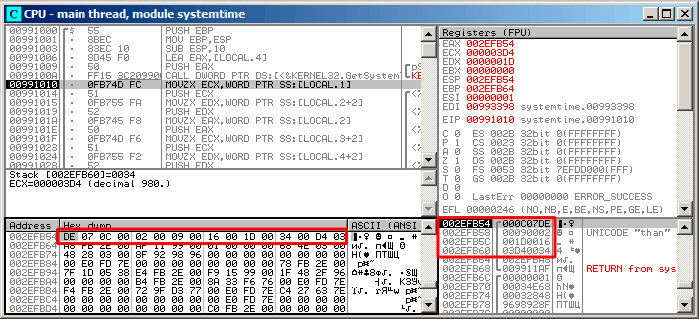
\includegraphics[scale=\FigScale]{patterns/15_structs/1_systemtime/olly_systemtime1.png}
\caption{\olly: \TT{GetSystemTime()} \RU{только что исполнилась}\EN{just executed}}
\label{fig:struct_olly_1}
\end{figure}

\RU{Точное системное время на моем компьютере, в которое исполнилась функция, это}
\EN{The system time of the function execution on my computer is} 9 \RU{декабря}\EN{december} 2014, 22:29:52:

\begin{figure}[H]
\centering
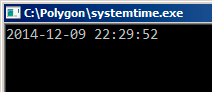
\includegraphics[scale=\NormalScale]{patterns/15_structs/1_systemtime/olly_systemtime2.png}
\caption{\olly: \RU{Вывод \printf}\EN{\printf output}}
\label{fig:struct_olly_2}
\end{figure}

\RU{Таким образом, в окне данных мы видим следующие 16 байт}\EN{So we see these 16 bytes in the
data window}: 
\begin{lstlisting}
DE 07 0C 00 02 00 09 00 16 00 1D 00 34 00 D4 03
\end{lstlisting}

\RU{Каждые два байта отражают одно поле структуры}\EN{Each two bytes represent one field of the structure}. 
\RU{А так как порядок байт (\gls{endianness}) \IT{little endian},
то в начале следует младший байт, затем старший}\EN{Since the \gls{endianness} is \IT{little endian}, 
we see the low byte first and then the high one}.
\RU{Следовательно, вот какие 16-битные числа сейчас записаны в памяти}
\EN{Hence, these are the values currently stored in memory}:

\begin{center}
\begin{tabular}{ | l | l | l | }
\hline
\headercolor{} \RU{Шестнадцатеричное число}\EN{Hexadecimal number} & 
\headercolor{} \RU{десятичное число}\EN{decimal number} & 
\headercolor{} \RU{имя поля}\EN{field name} \\
\hline
0x07DE & 2014	& wYear \\
\hline
0x000C & 12	& wMonth \\
\hline
0x0002 & 2	& wDayOfWeek \\
\hline
0x0009 & 9	& wDay \\
\hline
0x0016 & 22	& wHour \\
\hline
0x001D & 29	& wMinute \\
\hline
0x0034 & 52	& wSecond \\
\hline	
0x03D4 & 980	& wMilliseconds \\
\hline
\end{tabular}
\end{center}

\RU{В окне стека, видны те же значения, только они сгруппированы как 32-битные значения}
\EN{The same values are seen in the stack window, but they are grouped as 32-bit values}.

\RU{Затем}\EN{And then} \printf \RU{просто берет нужные значения и выводит их на консоль}
\EN{just takes the values it needs and outputs them to the console}.

\RU{Некоторые поля}\EN{Some values aren't output by} \printf \RU{не выводит} (\TT{wDayOfWeek} \AndENRU 
\TT{wMilliseconds}), \RU{но они находятся в памяти и доступны для использования.}
\EN{but they are in memory right now, available for use.}

\fi

\subsection{\RU{Замена структуры массивом}\EN{Replacing the structure with array}}

\RU{Тот факт, что поля структуры\EMDASH{}это просто переменные расположенные рядом, легко проиллюстрировать следующим образом.}%
\EN{The fact that the structure fields are just variables located side-by-side, can be easily demonstrated by doing the following.}
\RU{Глядя на описание структуры \TT{SYSTEMTIME}, можно переписать этот простой пример так:}%
\EN{Keeping in mind the \TT{SYSTEMTIME} structure description, it's possible to rewrite this simple example like this:}

\lstinputlisting{patterns/15_structs/1_systemtime/systemtime2.c}

\RU{Компилятор немного ворчит:}\EN{The compiler grumbles a bit:}

\begin{lstlisting}
systemtime2.c(7) : warning C4133: 'function' : incompatible types - from 'WORD [8]' to 'LPSYSTEMTIME'
\end{lstlisting}

\RU{Тем не менее, выдает такой код}\EN{But nevertheless, it produces this code}:

\lstinputlisting[caption=\NonOptimizing MSVC 2010]{patterns/15_structs/1_systemtime/systemtime2.asm}

\RU{И это работает так же}\EN{And it works just as the same}!

\RU{Любопытно что результат на ассемблере неотличим от предыдущего}
\EN{It is very interesting that the
result in assembly form cannot be distinguished from the result of the previous compilation}.
\RU{Таким образом, глядя на этот код, 
никогда нельзя сказать с уверенностью, была ли там объявлена структура, либо просто набор переменных.}
\EN{So by looking at this code, one cannot say for sure if there was a structure declared, or an array.} 

\RU{Тем не менее, никто в здравом уме делать так не будет.}
\EN{Nevertheless, no sane person would do it, }
\RU{Потому что это неудобно}\EN{as it is not convenient}. 
\RU{К тому же, иногда, поля в структуре могут меняться разработчиками, переставляться местами, \etc{}.}
\EN{Also the structure fields may be changed by developers, swapped, \etc{}.}

\ifdefined\IncludeOlly
\RU{С \olly этот пример изучать не будем, потому что он будет точно такой же, как и в случае со структурой.}%
\EN{We will not study this example in \olly, because it will be just the same as in the case with the structure.}
\fi

\section{\RU{Выделяем место для структуры через malloc()}\EN{Let's allocate space for a structure using malloc()}}
\label{struct_malloc_example}

\RU{Однако, бывает и так, что проще хранить структуры не в стеке, а в \glslink{heap}{куче}:}
\EN{Sometimes it is simpler to place structures not the in local stack, but in the \gls{heap}:}

\lstinputlisting{patterns/15_structs/2_using_malloc/systemtime_malloc.c}

\RU{Скомпилируем на этот раз с оптимизацией (\Ox) чтобы было проще увидеть то, что нам нужно.}
\EN{Let's compile it now with optimization (\Ox) so it would be easy see what we need.}

\lstinputlisting[caption=\Optimizing MSVC]{patterns/15_structs/2_using_malloc/systemtime_malloc.asm}

\index{\CStandardLibrary!malloc()}
\RU{Итак, \TT{sizeof(SYSTEMTIME) = 16}, именно столько байт выделяется при помощи \TT{malloc()}. 
Она возвращает указатель на только что выделенный блок памяти в \EAX, который копируется в \ESI. 
Win32 функция \TT{GetSystemTime()} обязуется сохранить состояние \ESI, 
поэтому здесь оно нигде не сохраняется и продолжает использоваться после вызова \TT{GetSystemTime()}.}
\EN{So, \TT{sizeof(SYSTEMTIME) = 16} and that is exact number of bytes to be allocated by \TT{malloc()}.
It returns a pointer to a freshly allocated memory block in the \EAX register,
which is then moved into the \ESI register.
\TT{GetSystemTime()} win32 function takes care of saving value in \ESI,
and that is why it is not saved here and continues to be used after the \TT{GetSystemTime()} call.}

\index{x86!\Instructions!MOVZX}
\RU{
Новая инструкция ~--- \MOVZX (\IT{Move with Zero eXtend}). 
Она нужна почти там же где и \MOVSX, 
только всегда очищает остальные биты в 0. Дело в том, что \printf требует 32-битный тип \Tint, 
а в структуре лежит WORD ~--- это 16-битный беззнаковый тип. Поэтому копируя значение из WORD в \Tint, 
нужно очистить биты от 16 до 31, иначе там будет просто случайный мусор, оставшийся от предыдущих действий 
с регистрами.}
\EN{New instruction~---\MOVZX (\IT{Move with Zero eXtend}).
It may be used in most cases as \MOVSX, but it sets the remaining bits to 0.
That's because \printf requires a 32-bit \Tint, but we got a WORD in the structure~---that
is 16-bit unsigned type.
That's why by copying the value from a WORD into \Tint{}, bits from 16 to 31 must be cleared, 
because a random noise may be there, which is left from the previous operations on the register(s).}

\RU{В этом примере можно также представить структуру как массив 8-и WORD-ов:}
\EN{In this example, it's possible to represent the structure as an array of 8 WORDs:}

\lstinputlisting{patterns/15_structs/2_using_malloc/systemtime_malloc2.c}

\RU{Получим такое}\EN{We get}:

\lstinputlisting[caption=\Optimizing MSVC]{patterns/15_structs/2_using_malloc/systemtime_malloc2.asm}

\RU{И снова мы получаем идентичный код, неотличимый от предыдущего.}
\EN{Again, we got the code cannot be distinguished from the previous one.}
\RU{Но и снова нужно отметить, что в реальности так лучше не делать, 
если только вы не знаете точно, что вы делаете.}
\EN{And again it should be noted, you haven't to do this in practice, unless you really know what you are doing.}


\ifx\LITE\undefined
\section{UNIX: struct tm}

% subsections here:
\subsection{Linux}

\RU{В Линуксе, для примера, возьмем структуру \TT{tm} из \TT{time.h}:}
\EN{Let's take the \TT{tm} structure from \TT{time.h} in Linux for example:}

\lstinputlisting{patterns/15_structs/3_tm_linux/GCC_tm.c}

\RU{Компилируем при помощи}\EN{Let's compile it in} GCC 4.4.1:

\lstinputlisting[caption=GCC 4.4.1]{patterns/15_structs/3_tm_linux/GCC_tm.asm.\LANG}

\RU{К сожалению, по какой-то причине, \IDA не сформировала названия локальных переменных в стеке. 
Но так как мы уже опытные реверсеры :-) то можем обойтись и без этого в таком простом примере.}
\EN{Somehow, \IDA did not write the local variables' names in the local stack.
But since we already are experienced reverse engineers :-) we may do it without this information in 
this simple example.}

\index{x86!\Instructions!LEA}
\RU{Обратите внимание на \TT{lea edx, [eax+76Ch]} ~--- эта инструкция прибавляет \TT{0x76C} (1900) к \EAX, 
но не модифицирует флаги. См. также соответствующий раздел об инструкции \LEA{}~(\myref{sec:LEA}).}
\EN{Please also pay attention to the \TT{lea edx, [eax+76Ch]}~---this instruction just adds \TT{0x76C} (1900) to value in \EAX,
but doesn't modify any flags. See also the relevant section about \LEA{}~(\myref{sec:LEA}).}

\ifdefined\IncludeGDB
\subsubsection{GDB}

\RU{Попробуем загрузить пример в GDB}\EN{Let's try to load the example into GDB}
\footnote{\RU{Результат работы \IT{date} немного подправлен в целях демонстрации.}%
\EN{The \IT{date} result is slightly corrected for demonstration purposes.}
\RU{Конечно же, в реальности, нельзя так быстро запустить GDB, чтобы значение секунд осталось бы таким же.}
\EN{Of course, it's not possible to run GDB that quickly, in the same second.}}:

\lstinputlisting[caption=GDB]{patterns/15_structs/3_tm_linux/GCC_tm_GDB.txt}

\RU{Мы легко находим нашу структуру в стеке}\EN{We can easily find our structure in the stack}.
\RU{Для начала, посмотрим, как она объявлена в}\EN{First, let's see how it's defined in} \IT{time.h}:

\begin{lstlisting}[caption=time.h, label=struct_tm]
struct tm
{
  int	tm_sec;
  int	tm_min;
  int	tm_hour;
  int	tm_mday;
  int	tm_mon;
  int	tm_year;
  int	tm_wday;
  int	tm_yday;
  int	tm_isdst;
};
\end{lstlisting}

\RU{Обратите внимание что здесь 32-битные \Tint вместо WORD в SYSTEMTIME}\EN{Pay attention that
32-bit \Tint is used here instead of WORD in SYSTEMTIME}.
\RU{Так что, каждое поле занимает 32-битное слово}\EN{So, each field occupies 32-bit}.

\RU{Вот поля нашей структуры в стеке}\EN{Here are the fields of our structure in the stack}:

\begin{lstlisting}
0xbffff0dc:	0x080484c3	0x080485c0	0x000007de	0x00000000
0xbffff0ec:	0x08048301	0x538c93ed	0x00000025 sec	0x0000000a min
0xbffff0fc:	0x00000012 hour	0x00000002 mday	0x00000005 mon 	0x00000072 year
0xbffff10c:	0x00000001 wday	0x00000098 yday	0x00000001 isdst0x00002a30
0xbffff11c:	0x0804b090	0x08048530	0x00000000	0x00000000
\end{lstlisting}

\RU{Либо же, в виде таблицы}\EN{Or as a table}:

\begin{center}
\begin{tabular}{ | l | l | l | }
\hline
\headercolor{} \RU{Шестнадцатеричное число}\EN{Hexadecimal number} & 
\headercolor{} \RU{десятичное число}\EN{decimal number} & 
\headercolor{} \RU{имя поля}\EN{field name} \\
\hline
0x00000025 & 37 	& tm\_sec \\
\hline
0x0000000a & 10 	& tm\_min \\
\hline
0x00000012 & 18 	& tm\_hour \\	
\hline
0x00000002 & 2 		& tm\_mday \\	
\hline
0x00000005 & 5 		& tm\_mon \\	
\hline
0x00000072 & 114 	& tm\_year \\
\hline
0x00000001 & 1 		& tm\_wday \\	
\hline
0x00000098 & 152 	& tm\_yday \\	
\hline
0x00000001 & 1 		& tm\_isdst \\
\hline
\end{tabular}
\end{center}

\RU{Как и в примере с}\EN{Just like} SYSTEMTIME (\myref{sec:SYSTEMTIME}), 
\RU{здесь есть и другие поля, готовые для использования, 
но в нашем примере они не используются, например,}
\EN{there are also other fields available that are not used, like} tm\_wday, tm\_yday, tm\_isdst.
\fi

\ifdefined\IncludeARM
\subsection{ARM}

\subsubsection{\OptimizingKeilVI (\ThumbMode)}

\RU{Этот же пример}\EN{Same example}:

\lstinputlisting[caption=\OptimizingKeilVI (\ThumbMode)]{patterns/15_structs/3_tm_linux/ARM/tm_ARM_keil_thumb.asm}

\subsubsection{\OptimizingXcodeIV (\ThumbTwoMode)}

\IDA \q{\RU{узнала}\EN{knows}} \RU{структуру}\EN{the} \TT{tm}\EN{ structure} 
(\RU{потому что}\EN{because} \IDA \q{\RU{знает}\EN{knows}} \RU{типы аргументов библиотечных функций, 
таких как}\EN{the types of the arguments of library functions like} \TT{localtime\_r()}), 
\RU{поэтому показала здесь обращения к отдельным элементам структуры и присвоила им имена}
\EN{so it shows here structure elements accesses and their names}.

\lstinputlisting[caption=\OptimizingXcodeIV (\ThumbTwoMode)]{patterns/15_structs/3_tm_linux/ARM/tm_ARM_xcode_thumb.asm}

\fi
\ifdefined\IncludeMIPS
\subsection{MIPS}

\lstinputlisting[caption=\Optimizing GCC 4.4.5 (IDA),numbers=left]{patterns/15_structs/3_tm_linux/MIPS/MIPS_O3_IDA.lst.\LANG}

\RU{Это тот пример, где branch delay slot-ы могут нас запутать.}
\EN{This is an example where the branch delay slots can confuse us.}
\RU{Например, в строке 35 есть инструкция \q{addiu \$a1, 1900}, добавляющая 1900 к числу года.}
\EN{For example, there is the instruction \q{addiu \$a1, 1900} at line 35 which adds 1900 to the year number.}
\RU{Но она исполняется перед исполнением соответствующей JALR в строке 34, не забыайте.}
\EN{It's executed before the corresponding JALR at line 34, do not forget about it.}

\fi
% subsection:
\ifdefined\IncludeGCC
\subsection{\RU{Структура как набор переменных}\EN{Structure as a set of values}}

\RU{Чтобы проиллюстрировать то что структура ~--- это просто набор переменных, лежащих в одном месте, 
переделаем немного пример, еще раз заглянув в описание структуры \IT{tm}}
\EN{In order to illustrate that the structure is just variables laying side-by-side in one place, 
let's rework our example while looking at the \IT{tm} structure definition again}: \lstref{struct_tm}.

\lstinputlisting{patterns/15_structs/3_tm_linux/as_array/GCC_tm2.c}

\index{\CStandardLibrary!localtime\_r()}
N.B. \RU{В \TT{localtime\_r} передается указатель именно на \TT{tm\_sec}, 
т.е. на первый элемент \q{структуры}.}
\EN{The pointer to the \TT{tm\_sec} field is passed into \TT{localtime\_r}, i.e., 
to the first element of the \q{structure}.}

\RU{В итоге, и этот компилятор поворчит}\EN{The compiler warns us}:

\begin{lstlisting}[caption=GCC 4.7.3]
GCC_tm2.c: In function 'main':
GCC_tm2.c:11:5: warning: passing argument 2 of 'localtime_r' from incompatible pointer type [enabled by default]
In file included from GCC_tm2.c:2:0:
/usr/include/time.h:59:12: note: expected 'struct tm *' but argument is of type 'int *'
\end{lstlisting}

\RU{Тем не менее, сгенерирует такое}\EN{But nevertheless, it generates this}:

\lstinputlisting[caption=GCC 4.7.3]{patterns/15_structs/3_tm_linux/as_array/GCC_tm2.asm}

\RU{Этот код почти идентичен уже рассмотренному, и нельзя сказать, была ли структура
в оригинальном исходном коде либо набор переменных.}\EN{This code is identical to what we saw previously and it is
not possible to say, was it a structure in original source code or just a pack of variables.}

\RU{И это работает}\EN{And this works}. 
\RU{Однако, в реальности так лучше не делать}\EN{However, it is not recommended to do this in practice}. 
\RU{Обычно, неоптимизируюий компилятор располагает переменные в локальном
стеке в том же порядке, в котором они объявляются в функции.}
\EN{Usually, non-optimizing compilers allocates variables in the local stack in the 
same order as they were declared in the function.}
\RU{Тем не менее, никакой гарантии нет.}
\EN{Nevertheless, there is no guarantee.}

\RU{Кстати, какой-нибудь другой компилятор может предупредить, что переменные}
\EN{By the way, some other compiler may warn about the} \TT{tm\_year}, \TT{tm\_mon}, \TT{tm\_mday},
\TT{tm\_hour}, \TT{tm\_min}\RU{, но не}\EN{ variables, but not} \TT{tm\_sec}\RU{, используются без инициализации}
\EN{ are used without being initialized}.
\RU{Действительно, ведь компилятор не знает что они будут заполнены при вызове функции}
\EN{Indeed, the compiler is not aware that these are to be filled by} 
\TT{localtime\_r()}\EN{ function}.

\EN{We chose this example, since all structure fields are of type \Tint.}%
\RU{Мы выбрали именно этот пример для иллюстрации, потому что все члены структуры имеют тип \Tint.}
\RU{Это не сработает, если поля структуры будут иметь размер 16 бит (\TT{WORD}), как в случае
со структурой \TT{SYSTEMTIME}}\EN{This would not work if structure fields are 16-bit (\TT{WORD}), 
like in the case of the \TT{SYSTEMTIME} structure}\EMDASH{}\TT{GetSystemTime()} 
\RU{заполнит их неверно}\EN{will fill them incorrectly} 
(\RU{потому что локальные переменные выровнены по 32-битной границе}
\EN{because the local variables are aligned on a 32-bit boundary}).
\RU{Читайте об этом в следующей секции}\EN{Read more about it in next section}: 
\q{\StructurePackingSectionName} (\myref{structure_packing}).

\RU{Так что, структура\EMDASH{}это просто набор переменных лежащих в одном месте, рядом.}%
\EN{So, a structure is just a pack of variables laying on one place, side-by-side.}
\RU{Можно было бы сказать, что структура\EMDASH{}это инструкция компилятору, заставляющая его удерживать переменные в одном месте.}%
\EN{We could say that the structure is the instruction to the compiler, directing it to hold variables in one place.}
\RU{Кстати, когда-то, в очень ранних версиях Си (перед 1972) структур не было вовсе}%
\EN{By the way, in some very early C versions (before 1972), there were no structures at all} \cite{Ritchie:1993:DCL:155360.155580}.

\RU{Здесь нет примера с отладчиком: потому что он будет полностью идентичным тому, что вы уже видели.}%
\EN{There is no debugger example here: it is just the same as you already saw.}

\subsection{\RU{Структура как массив 32-битных слов}\EN{Structure as an array of 32-bit words}}

\lstinputlisting{patterns/15_structs/3_tm_linux/as_array/GCC_tm3.c}

\RU{Мы просто приводим (\IT{cast}) указатель на структуру к массиву \Tint{}-ов}%
\EN{We just \IT{cast} a pointer to structure to an array of \Tint{}'s}.
\RU{И это работает}\EN{And that works}!
\RU{Запускаем пример}\EN{We run the example at} 23:51:45 26-July-2014.

\begin{lstlisting}[label=GCC_tm3_output]
0x0000002D (45)
0x00000033 (51)
0x00000017 (23)
0x0000001A (26)
0x00000006 (6)
0x00000072 (114)
0x00000006 (6)
0x000000CE (206)
0x00000001 (1)
\end{lstlisting}

\RU{Переменные здесь в том же порядке, в котором они перечислены в определении структуры}\EN{The variables here 
are in the same order as they are enumerated in the definition of the structure}: \myref{struct_tm}.

\RU{Вот как это компилируется}\EN{Here is how it gets compiled}:

\lstinputlisting[caption=\Optimizing GCC 4.8.1]{patterns/15_structs/3_tm_linux/as_array/GCC_tm3.lst.\LANG}

\RU{И действительно: место в локальном стеке в начале используется как структура, затем как массив.}
\EN{Indeed: the space in the local stack is first treated as a structure, and then it's treated as an array.}

\RU{Возможно даже модифицировать поля структуры через указатель.}
\EN{It's even possible to modify the fields of the structure through this pointer.}

\RU{И снова, это сомнительный хакерский способ, который не рекомендуется использовать в настоящем коде.}
\EN{And again, it's dubiously hackish way to do things, not recommended for use in production code.}

\ifdefined\IncludeExercises
\myparagraph{\Exercise}

\RU{В качестве упражнения, попробуйте модифицировать (увеличить на 1) 
текущий номер месяца обращаясь со структурой как с массивом.}
\EN{As an exercise, try to modify (increase by 1) the current month number, treating the structure as 
an array.}
\fi

\subsection{\RU{Структура как массив байт}\EN{Structure as an array of bytes}}

\RU{Можно пойти еще дальше. Можно привести (\IT{cast}) указатель к массиву байт и вывести его:}%
\EN{We can go even further. Let's \IT{cast} the pointer to an array of bytes and dump it:}

\lstinputlisting{patterns/15_structs/3_tm_linux/as_array/GCC_tm4.c}

\begin{lstlisting}
0x2D 0x00 0x00 0x00 
0x33 0x00 0x00 0x00 
0x17 0x00 0x00 0x00 
0x1A 0x00 0x00 0x00 
0x06 0x00 0x00 0x00 
0x72 0x00 0x00 0x00 
0x06 0x00 0x00 0x00 
0xCE 0x00 0x00 0x00 
0x01 0x00 0x00 0x00 
\end{lstlisting}

\RU{Мы также запускаем этот пример в}\EN{We also run this example also at} 23:51:45 26-July-2014
\footnote{\EN{The time and date are the same for demonstration purposes. Byte values are fixed up.}%
\RU{Время и дата такая же в целях демонстрации. Значения байт были подправлены.}}.
\RU{Переменные точно такие же, как и в предыдущем выводе}\EN{The values are just the same as in the previous dump} 
(\myref{GCC_tm3_output}), \RU{и конечно, младший байт идет в самом начале, потому что это архитектура 
little-endian}\EN{and of course, the lowest byte goes first, because this is a little-endian architecture} 
(\myref{sec:endianness}).

\lstinputlisting[caption=\Optimizing GCC 4.8.1]{patterns/15_structs/3_tm_linux/as_array/GCC_tm4.lst.\LANG}
\fi


\fi
\section{\StructurePackingSectionName}
\label{structure_packing}

\RU{Достаточно немаловажный момент, это упаковка полей в структурах\footnote{См. также: \URLWPDA}.}
\EN{One important thing is fields packing in structures\footnote{See also: \URLWPDA}.}

\RU{Возьмем простой пример:}\EN{Let's take a simple example:}

\lstinputlisting{patterns/15_structs/4_packing/packing.c}

\RU{Как видно, мы имеем два поля \Tchar (занимающий один байт) и еще два ~--- \Tint (по 4 байта).}
\EN{As we see, we have two \Tchar fields (each is exactly one byte) and two more~---\Tint (each --- 4 bytes).}

% subsections:

\subsection{x86}

\RU{Компилируется это все в:}\EN{This compiles to:}

\lstinputlisting[caption=MSVC 2012 /GS- /Ob0,label=src:struct_packing_4,numbers=left]{patterns/15_structs/4_packing/packing.asm.\LANG}

\RU{Кстати, мы передаем всю структуру, но в реальности, как видно, структура в начале копируется
во временную структуру (выделение места под нее в стеке происходит в строке 10,
а все 4 поля, по одному, копируются в строках 12 \ldots\ 19), 
затем передается только указатель на нее (или адрес).}
\EN{We pass the structure as a whole, but in fact, as we can see, the structure
is being copied to a temporary one (a place in stack is allocated in line 10 for it,
and then all 4 fields, one by one, are copied in lines 12 \ldots\ 19), 
and then its pointer (address) is to be passed.}
\RU{Структура копируется, потому что неизвестно, будет ли функция \ttf модифицировать структуру или нет.
И если да, то структура внутри \main должна остаться той же.}
\EN{The structure is copied because it's not known whether the \ttf{} 
function going to modify the structure or not.
If it gets changed, then the structure in \main has to remain as it was.}
\RU{Мы могли бы использовать указатели на \CCpp, и итоговый код был бы почти такой же,
только копирования не было бы.}
\EN{We could use \CCpp pointers, and the resulting code will be almost the same, but without
the copying.}

\RU{Мы видим здесь что адрес каждого поля в структуре выравнивается по 4-байтной границе. 
Так что каждый \Tchar здесь занимает те же 4 байта что и \Tint. Зачем? 
Затем что процессору удобнее обращаться по таким адресам и кэшировать данные из памяти.}
\EN{As we can see, each field's address is aligned on a 4-byte boundary.
That's why each \Tchar occupies 4 bytes here (like \Tint). Why?
Because it is easier for the CPU to access memory at aligned addresses and to cache data from it.}

\RU{Но это не экономично по размеру данных.}\EN{However, it is not very economical.}

\RU{Попробуем скомпилировать тот же исходник с опцией}\EN{Let's try to compile it with option} (\TT{/Zp1}) 
(\IT{/Zp[n] pack structures on n-byte boundary}).

\lstinputlisting[caption=MSVC 2012 /GS- /Zp1,label=src:struct_packing_1,numbers=left]
{patterns/15_structs/4_packing/packing_msvc_Zp1.asm.\LANG}

\RU{Теперь структура занимает 10 байт и все \Tchar занимают по байту. Что это дает? 
Экономию места. Недостаток ~--- процессор будет обращаться к этим полям не так эффективно 
по скорости, как мог бы.}
\EN{Now the structure takes only 10 bytes and each \Tchar value takes 1 byte. What does it give to us?
Size economy. And as drawback~---the CPU accessing these fields slower than it could.}

\label{short_struct_copying_using_MOV}
\RU{Структура так же копируется в \main. Но не по одному полю, а 10 байт, при помощи трех
пар \MOV.}
\EN{The structure is also copied in \main. Not field-by-field, but directly 10 bytes, using three pairs
of \MOV.}
\RU{Почему не 4?}\EN{Why not 4?}
\RU{Компилятор рассудил, что будет лучше скопировать 10 байт
при помощи 3 пар \MOV, чем копировать два 32-битных слова и два байта при помощи 4 пар \MOV.}
\EN{The compiler decided that it's better to copy 10 bytes using 3 \MOV pairs than to copy two 32-bit words
and two bytes using 4 \MOV pairs.}
\ifx\LITE\undefined
\RU{Кстати, подобная реализация копирования при помощи \MOV взамен вызова функции \TT{memcpy()}, например, это
очень распространенная практика, потому что это в любом случае работает быстрее чем вызов \TT{memcpy()} ---
если речь идет о коротких блоках, конечно: \myref{copying_short_blocks}.}
\EN{By the way, such copy implementation using \MOV instead of calling the \TT{memcpy()} function is widely
used, because it's faster than a call to \TT{memcpy()}---for short blocks, of course:
\myref{copying_short_blocks}.}
\fi

\RU{Как нетрудно догадаться, если структура используется много в каких исходниках и объектных файлах, 
все они должны быть откомпилированы с одним и тем же соглашением об упаковке структур.}
\EN{As it can be easily guessed, if the structure is used in many source and object files,
all these must be compiled with the same convention about structures packing.}

\newcommand{\FNURLMSDNZP}{\footnote{\href{http://go.yurichev.com/17067}
{MSDN: Working with Packing Structures}}}
\newcommand{\FNURLGCCPC}{\footnote{\href{http://go.yurichev.com/17068}
{Structure-Packing Pragmas}}}

\RU{Помимо ключа MSVC \TT{/Zp}, указывающего, по какой границе упаковывать поля структур, есть также 
опция компилятора \TT{\#pragma pack}, её можно указывать прямо в исходнике. 
Это справедливо и для MSVC\FNURLMSDNZP и GCC\FNURLGCCPC{}.}
\EN{Aside from MSVC \TT{/Zp} option which sets how to align each structure field, there is also
the \TT{\#pragma pack} compiler option, which can be defined right in the source code.
It is available in both MSVC\FNURLMSDNZP and GCC\FNURLGCCPC{}.}

\RU{Давайте теперь вернемся к \TT{SYSTEMTIME}, которая состоит из 16-битных полей. 
Откуда наш компилятор знает что их надо паковать по однобайтной границе?}
\EN{Let's get back to the \TT{SYSTEMTIME} structure that consists of 16-bit fields.
How does our compiler know to pack them on 1-byte alignment boundary?}

\RU{В файле \TT{WinNT.h} попадается такое:}\EN{\TT{WinNT.h} file has this:}

\begin{lstlisting}[caption=WinNT.h]
#include "pshpack1.h"
\end{lstlisting}

\RU{И такое:}\EN{And this:}

\begin{lstlisting}[caption=WinNT.h]
#include "pshpack4.h"                   // 4 byte packing is the default
\end{lstlisting}

\RU{Сам файл PshPack1.h выглядит так:}\EN{The file PshPack1.h looks like:}

\begin{lstlisting}[caption=PshPack1.h]
#if ! (defined(lint) || defined(RC_INVOKED))
#if ( _MSC_VER >= 800 && !defined(_M_I86)) || defined(_PUSHPOP_SUPPORTED)
#pragma warning(disable:4103)
#if !(defined( MIDL_PASS )) || defined( __midl )
#pragma pack(push,1)
#else
#pragma pack(1)
#endif
#else
#pragma pack(1)
#endif
#endif /* ! (defined(lint) || defined(RC_INVOKED)) */
\end{lstlisting}

\RU{Собственно, так и задается компилятору, как паковать объявленные после \TT{\#pragma pack} структуры.}
\EN{This tell the compiler how to pack the structures defined after \TT{\#pragma pack}.}

\ifdefined\IncludeOlly
\input{patterns/15_structs/4_packing/olly.tex}
\fi


\ifdefined\IncludeARM
\subsection{ARM}

\subsubsection{\OptimizingKeilVI (\ThumbMode)}

\lstinputlisting[caption=\OptimizingKeilVI (\ThumbMode)]{patterns/15_structs/4_packing/packing_Keil_thumb.asm}

\RU{Как мы помним, здесь передается не указатель на структуру, а сама структура, а так как в ARM первые 4 аргумента
функции передаются через регистры, то поля структуры передаются через}
\EN{As we may recall, here a structure is passed instead of pointer to one,
and since the first 4 function arguments in ARM are passed via registers,
the structure's fields are passed via} \TT{R0-R3}.

\index{ARM!\Instructions!LDRB}
\index{x86!\Instructions!MOVSX}
\RU{Инструкция }\TT{LDRB} \RU{загружает один байт из памяти и расширяет до 32-бит учитывая знак.}
\EN{loads one byte from memory and extends it to 32-bit, taking its sign into account.}
\RU{Это то же что и инструкция}\EN{This is similar to} \MOVSX \RU{в}\EN{in} x86.
\RU{Она здесь применяется для загрузки полей}\EN{Here it is used to load fields} $a$ \AndENRU $c$ 
\RU{из структуры}\EN{from the structure}.

\index{Function epilogue}
\RU{Еще что бросается в глаза, так это то что вместо эпилога функции, переход на эпилог другой функции!}
\EN{One more thing we spot easily is that instead of function epilogue, there is jump to another function's epilogue!}
\RU{Действительно, то была совсем другая, не относящаяся к этой, функция, однако, она имела точно такой же
эпилог}\EN{Indeed, that was quite different function, not related in any way to ours, however, it has exactly
the same epilogue} 
(\RU{видимо, тоже хранила в стеке 5 локальных переменных}\EN{probably because, it hold 5 local variables too} 
($5*4=0x14$)).
\RU{К тому же, она находится рядом (обратите внимание на адреса).}
\EN{Also it is located nearby (take a look at the addresses).}
\RU{Действительно, нет никакой разницы, какой эпилог исполнять, если он работает так же, как нам нужно.}
\EN{Indeed, it doesn't matter which epilogue gets executed,
if it works just as we need.}
\RU{Keil решил использовать часть другой функции, вероятно, из-за экономии.}
\EN{Apparently, Keil decides to reuse a part of another function to economize.}
\RU{Эпилог занимает 4 байта, а переход ~--- только 2.}
\EN{The epilogue takes 4 bytes while jump~---only 2.}

\subsubsection{ARM + \OptimizingXcodeIV (\ThumbTwoMode)}

\lstinputlisting[caption=\OptimizingXcodeIV (\ThumbTwoMode)]{patterns/15_structs/4_packing/packing_Xcode_thumb.asm}

\index{ARM!\Instructions!SXTB}
\index{x86!\Instructions!MOVSX}
\TT{SXTB} (\IT{Signed Extend Byte}) \RU{это также аналог}\EN{is analogous to} \MOVSX \InENRU x86.
\RU{Всё остальное ~--- так же.}\EN{All the rest~---just the same.}

\fi
\ifdefined\IncludeMIPS
\subsection{MIPS}
\label{MIPS_structure_big_endian}

\lstinputlisting[caption=\Optimizing GCC 4.4.5 (IDA),numbers=left]{patterns/15_structs/4_packing/MIPS_O3_IDA.lst}

\RU{Поля структуры приходят в регистрах \$A0..\$A3 и затем перетасовываются в регистры \$A1..\$A4 для \printf.}
\EN{Structure fields come in registers \$A0..\$A3 and then get reshuffled into \$A1..\$A4 for \printf.}
\RU{Но здесь есть две инструкции SRA (\q{Shift Word Right Arithmetic}), которые готовят поля типа \Tchar.}
\EN{But there are two SRA (\q{Shift Word Right Arithmetic}) instructions, which prepare \Tchar fields.}
\RU{Почему}\EN{Why}?
\RU{По умолчанию, MIPS это big-endian архитектура \myref{sec:endianness}, и Debian Linux в котором мы работаем, также big-endian.}
\EN{MIPS is a big-endian architecture by default \myref{sec:endianness}, and the Debian Linux we work in is big-endian as well.}
\RU{Так что когда один байт расположен в 32-битном элементе структуры, он занимает биты 31..24.}
\EN{So when byte variables are stored in 32-bit structure slots, they occupy the high 31..24 bits.}
\RU{И когда переменную типа \Tchar нужно расширить до 32-битного значения, она должна быть сдвинута вправо
на 24 бита.}
\EN{And when a \Tchar variable needs to be extended into a 32-bit value, it must be shifted right by 24 bits.}
\RU{\Tchar это знаковый тип, так что здесь нужно использовать арифметический сдвиг вместо логического.}
\EN{\Tchar is a signed type, so an arithmetical shift is used here instead of logical.}

\fi

\subsection{\RU{Еще кое-что}\EN{One more word}}

\EN{Passing a structure as a function argument (instead of a passing pointer to structure) is the same
as passing all structure fields one by one.}
\RU{Передача структуры как аргумент функции (вместо передачи указателя на структуру) это то же
что и передача всех полей структуры по одному.}
\EN{If the structure fields are packed by default, the f() function can be rewritten as:}
\RU{Если поля в структуре пакуются по умолчанию, то функцию f() можно переписать так:}

\begin{lstlisting}
void f(char a, int b, char c, int d)
{
    printf ("a=%d; b=%d; c=%d; d=%d\n", a, b, c, d);
};
\end{lstlisting}

\RU{И в итоге будет такой же код}\EN{And that leads to the same code}.

\section{\RU{Вложенные структуры}\EN{Nested structures}}

\RU{Теперь, как насчет ситуаций, когда одна структура определена внутри другой структуры?}
\EN{Now what about situations when one structure is defined inside of another?}

\lstinputlisting{patterns/15_structs/5_nested/nested.c}

\dots \RU{в этом случае, оба поля \TT{inner\_struct} просто будут располагаться между полями a,b и d,e в 
\TT{outer\_struct}.}
\EN{in this case, both \TT{inner\_struct} fields are to be placed between the a,b and d,e fields of
the \TT{outer\_struct}.}

\RU{Компилируем}\EN{Let's compile} (MSVC 2010):

\lstinputlisting[caption=\Optimizing MSVC 2010 /Ob0]{patterns/15_structs/5_nested/nested_msvc.asm}

\RU{Очень любопытный момент в том, что глядя на этот код на ассемблере, мы даже не видим, 
что была использована какая-то еще другая структура внутри этой!
Так что, пожалуй, можно сказать, что все вложенные структуры в итоге разворачиваются в одну, \IT{линейную} 
или \IT{одномерную} структуру.}
\EN{One curious thing here is that by looking onto this assembly code, we do not even see that
another structure was used inside of it!
Thus, we would say, nested structures are unfolded into \IT{linear} or \IT{one-dimensional} structure.}

\RU{Конечно, если заменить объявление \TT{struct inner\_struct c;} на \TT{struct inner\_struct *c;} 
(объявляя таким образом указатель), ситуация будет совсем иная.}
\EN{Of course, if we replace the \TT{struct inner\_struct c;} declaration with \TT{struct inner\_struct *c;} 
(thus making a pointer here) the situation will be quite different.}
% FIXME1: нарисовать вложенную структуру и развернутую

\ifdefined\IncludeOlly
\clearpage
\subsection{\olly}
\index{\olly}

\RU{Загружаем пример в}\EN{Let's load the example into} \olly \RU{и смотрим на}\EN{and take a look at} 
\TT{outer\_struct} \RU{в памяти}\EN{in memory}:

\begin{figure}[H]
\centering
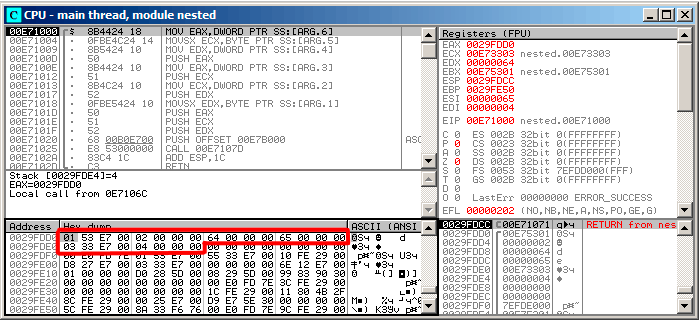
\includegraphics[scale=\FigScale]{patterns/15_structs/5_nested/olly.png}
\caption{\olly: \RU{Перед исполнением \printf}\EN{Before \printf execution}}
\label{fig:nested_olly}
\end{figure}

\RU{Вот как расположены значения в памяти}\EN{That's how the values are located in memory}:
\begin{itemize}
\item \IT{(outer\_struct.a)} \RU{(байт) 1 + 3 байта случайного мусора}\EN{(byte) 1 + 3 bytes of random garbage};
\item \IT{(outer\_struct.b)} (\RU{32-битное слово}\EN{32-bit word}) 2;
\item \IT{(inner\_struct.a)} (\RU{32-битное слово}\EN{32-bit word}) 0x64 (100);
\item \IT{(inner\_struct.b)} (\RU{32-битное слово}\EN{32-bit word}) 0x65 (101);
\item \IT{(outer\_struct.d)} \RU{(байт) 3 + 3 байта случайного мусора}\EN{(byte) 3 + 3 bytes of random garbage};
\item \IT{(outer\_struct.e)} (\RU{32-битное слово}\EN{32-bit word}) 4.
\end{itemize}

\fi


\section{\RU{Работа с битовыми полями в структуре}\EN{Bit fields in a structure}}

\subsection{\RU{Пример CPUID}\EN{CPUID example}}

\RU{Язык \CCpp позволяет указывать, сколько именно бит отвести для каждого поля структуры. 
Это удобно если нужно экономить место в памяти. К примеру, для переменной типа \Tbool достаточно одного бита.
Но, это не очень удобно, если нужна скорость.}
\EN{The \CCpp language allows to define the exact number of bits for each structure field.
It is very useful if one needs to save memory space. 
For example, one bit is enough for a \Tbool variable.
But of course, it is not rational if speed is important.}
% FIXME!
% another use of this is to parse binary protocols/packets, for example
% the definition of struct iphdr in include/linux/ip.h

\newcommand{\FNCPUID}{\footnote{\href{http://go.yurichev.com/17069}{wikipedia}}}

\index{x86!\Instructions!CPUID}
\label{cpuid}
\RU{Рассмотрим пример с инструкцией \CPUID\FNCPUID. 
Эта инструкция возвращает информацию о том, какой процессор имеется в наличии и какие возможности он имеет.}
\EN{Let's consider the \CPUID\FNCPUID instruction example.
This instruction returns information about the current CPU and its features.}

\RU{Если перед исполнением инструкции в \EAX будет 1, 
то \CPUID вернет упакованную в \EAX такую информацию о процессоре:}
\EN{If the \EAX is set to 1 before the instruction's execution, 
\CPUID returning this information packed into the \EAX register:}

\begin{center}
\begin{tabular}{ | l | l | }
\hline
3:0 (4 \bitsENRU)& Stepping \\
7:4 (4 \bitsENRU) & Model \\
11:8 (4 \bitsENRU) & Family \\
13:12 (2 \bitsENRU) & Processor Type \\
19:16 (4 \bitsENRU) & Extended Model \\
27:20 (8 \bitsENRU) & Extended Family \\
\hline
\end{tabular}
\end{center}

\newcommand{\FNGCCAS}{\footnote{\href{http://go.yurichev.com/17070}
{\RU{Подробнее о встроенном ассемблере GCC}\EN{More about internal GCC assembler}}}}

\RU{MSVC 2010 имеет макрос для \CPUID, а GCC 4.4.1 ~--- нет. 
Поэтому для GCC сделаем эту функцию сами, используя его встроенный ассемблер\FNGCCAS.}
\EN{MSVC 2010 has \CPUID macro, but GCC 4.4.1 does not.
So let's make this function by ourselves for GCC with the help of its built-in assembler\FNGCCAS.}

\lstinputlisting{patterns/15_structs/6_bitfields/cpuid/CPUID.c}

\RU{После того как \CPUID заполнит \EAX/\EBX/\ECX/\EDX, у нас они отразятся в массиве \TT{b[]}. 
Затем, мы имеем указатель на структуру \TT{CPUID\_1\_EAX}, и мы указываем его на значение 
\EAX из массива \TT{b[]}.}
\EN{After \CPUID fills \EAX/\EBX/\ECX/\EDX, these registers are to be written in the \TT{b[]} array.
Then, we have a pointer to the \TT{CPUID\_1\_EAX} structure and we point it to the value in \EAX from the \TT{b[]} array.}

\RU{Иными словами, мы трактуем 32-битный \Tint как структуру.}
\EN{In other words, we treat a 32-bit \Tint value as a structure.}
\RU{Затем мы читаем отдельные биты из структуры.}\EN{Then we read specific bits from the structure.}

\subsubsection{MSVC}

\RU{Компилируем в MSVC 2008 с опцией \Ox}\EN{Let's compile it in MSVC 2008 with \Ox option}:

\lstinputlisting[caption=\Optimizing MSVC 2008]{patterns/15_structs/6_bitfields/cpuid/CPUID_msvc_Ox.asm}

\index{x86!\Instructions!SHR}
\RU{Инструкция \TT{SHR} сдвигает значение из \EAX на то количество бит, 
которое нужно \IT{пропустить}, то есть, мы игнорируем некоторые биты \IT{справа}.}
\EN{The \TT{SHR} instruction shifting the value in \EAX by the number of bits that must be
\IT{skipped}, e.g., we ignore some bits \IT{at the right side}.}

\index{x86!\Instructions!AND}
\RU{А инструкция \AND очищает биты \IT{слева} которые нам не нужны, или же, говоря иначе, 
она оставляет по маске только те биты в \EAX, которые нам сейчас нужны.}
\EN{The \AND instruction clears the unneeded bits \IT{on the left}, or, in other words, 
leaves only those bits in the \EAX register we need.}

\ifdefined\IncludeOlly
\input{patterns/15_structs/6_bitfields/cpuid/olly.tex}
\fi

\ifdefined\IncludeGCC
\subsubsection{GCC}

\RU{Попробуем GCC 4.4.1 с опцией \Othree.}\EN{Let's try GCC 4.4.1 with \Othree option.}

\lstinputlisting[caption=\Optimizing GCC 4.4.1]{patterns/15_structs/6_bitfields/cpuid/CPUID_gcc_O3.asm}

\RU{Практически, то же самое. Единственное что стоит отметить это то, что GCC решил зачем-то объединить 
вычисление \TT{extended\_model\_id} и \TT{extended\_family\_id} в один блок, 
вместо того чтобы вычислять их перед соответствующим вызовом \printf.}
\EN{Almost the same.
The only thing worth noting is that GCC somehow combines the calculation of
\TT{extended\_model\_id} and \TT{extended\_family\_id} into one block,
instead of calculating them separately before each \printf call.}
\fi

\ifx\LITE\undefined
\subsection{\WorkingWithFloatAsWithStructSubSubSectionName}
\label{sec:floatasstruct}

\RU{Как уже ранее указывалось в секции о FPU~(\myref{sec:FPU}), 
и \Tfloat и \Tdouble содержат в себе \IT{знак}, \IT{мантиссу} и \IT{экспоненту}. 
Однако, можем ли мы работать с этими полями напрямую? Попробуем с \Tfloat.}
\EN{As we already noted in the section about FPU~(\myref{sec:FPU}), 
both \Tfloat and \Tdouble types consist of a \IT{sign}, 
a \IT{significand} (or \IT{fraction}) and an \IT{exponent}.
But will we be able to work with these fields directly? Let's try this with \Tfloat.}

\input{float_IEEE754.tex}

\lstinputlisting{patterns/15_structs/6_bitfields/float/float.c.\LANG}

\RU{Структура \TT{float\_as\_struct} занимает в памяти столько же места сколько и \Tfloat, 
то есть 4 байта или 32 бита.}
\EN{The \TT{float\_as\_struct} structure occupies the same amount of  memory as \Tfloat, i.e., 4 bytes or 32 bits.}

\RU{Далее мы выставляем во входящем значении отрицательный знак, 
а также прибавляя двойку к экспоненте, мы тем 
самым умножаем всё значение на \TT{$2^2$}, то есть на 4.}
\EN{Now we are setting the negative sign in the input value and also, by adding 2 to the exponent, 
we thereby multiply the whole number by \TT{$2^2$}, i.e., by 4.}

\RU{Компилируем в MSVC 2008 без включенной оптимизации:}
\EN{Let's compile in MSVC 2008 without optimization turned on:}

\lstinputlisting[caption=\NonOptimizing MSVC 2008]{patterns/15_structs/6_bitfields/float/float_msvc.asm.\LANG}

\RU{Слегка избыточно. В версии скомпилированной с флагом \Ox нет вызовов \TT{memcpy()}, 
там работа происходит сразу с переменной \TT{f}. Но по неоптимизированной версии будет проще понять.}
\EN{A bit redundant.
If it was compiled with \Ox flag there would be no \TT{memcpy()} call,
the \TT{f} variable is used directly.
But it is easier to understand by looking at the unoptimized version.}

\RU{А что сделает GCC 4.4.1 с опцией \Othree?}\EN{What would GCC 4.4.1 with \Othree do?}

\lstinputlisting[caption=\Optimizing GCC 4.4.1]{patterns/15_structs/6_bitfields/float/float_gcc_O3.asm.\LANG}

\RU{Да, функция \ttf в целом понятна. Однако, что интересно, еще при компиляции, 
не взирая на мешанину с полями структуры, GCC умудрился вычислить результат функции \TT{f(1.234)} еще
во время компиляции и сразу подставить его в аргумент для \printf{}!}
\EN{The \ttf function is almost understandable. However, what is interesting is that GCC was able to calculate
the result of \TT{f(1.234)} during compilation despite all this hodge-podge with the structure fields
and prepared this argument to \printf{} as precalculated at compile time!}

\fi

\ifdefined\IncludeExercises
\section{\Exercises}

\subsection{\Exercise \#1}
\label{exercise_struct_1}

\href{http://go.yurichev.com/17217}{Linux x86 (beginners.re)}\footnote{GCC 4.8.1 -O3}\\
\href{http://go.yurichev.com/17218}{Linux MIPS (beginners.re)}\footnote{GCC 4.4.5 -O3}\\
\EN{This program for Linux x86 and Linux MIPS opens a file and prints a number. What is this number?}
\RU{Эта программа для Linux x86 и Linux MIPS открывает файл и выводит какое-то число. Что это за число?}

\Answer{}: \myref{exercise_solutions_struct_1}.

\subsection{\Exercise \#2}
\label{exercise_struct_2}

\EN{This function takes some structure on input and does something. Try to reverse engineer structure field types.
Function contents may be ignored for the moment.}
\RU{Эта функция берет какую-то структуру на вход и делает что-то. Попробуйте разобраться, поля каких типов 
присутствуют в структуре. Самое содержимое функции можно пока игнорировать.}

\begin{lstlisting}[caption=\Optimizing MSVC 2010]
$SG2802	DB	'%f', 0aH, 00H
$SG2803	DB	'%c, %d', 0aH, 00H
$SG2805	DB	'error #2', 0aH, 00H
$SG2807	DB	'error #1', 0aH, 00H

__real@405ec00000000000 DQ 0405ec00000000000r	; 123
__real@407bc00000000000 DQ 0407bc00000000000r	; 444

_s$ = 8
_f	PROC
	push	esi
	mov	esi, DWORD PTR _s$[esp]
	cmp	DWORD PTR [esi], 1000
	jle	SHORT $LN4@f
	cmp	DWORD PTR [esi+4], 10
	jbe	SHORT $LN3@f
	fld	DWORD PTR [esi+8]
	sub	esp, 8
	fmul	QWORD PTR __real@407bc00000000000
	fld	QWORD PTR [esi+16]
	fmul	QWORD PTR __real@405ec00000000000
	faddp	ST(1), ST(0)
	fstp	QWORD PTR [esp]
	push	OFFSET $SG2802 ; '%f'
	call	_printf
	movzx	eax, BYTE PTR [esi+25]
	movsx	ecx, BYTE PTR [esi+24]
	push	eax
	push	ecx
	push	OFFSET $SG2803 ; '%c, %d'
	call	_printf
	add	esp, 24
	pop	esi
	ret	0
$LN3@f:
	pop	esi
	mov	DWORD PTR _s$[esp-4], OFFSET $SG2805 ; 'error #2'
	jmp	_printf
$LN4@f:
	pop	esi
	mov	DWORD PTR _s$[esp-4], OFFSET $SG2807 ; 'error #1'
	jmp	_printf
_f	ENDP
\end{lstlisting}

\begin{lstlisting}[caption=\NonOptimizingKeilVI (\ARMMode)]
f PROC
        PUSH     {r4-r6,lr}
        MOV      r4,r0
        LDR      r0,[r0,#0]
        CMP      r0,#0x3e8
        ADRLE    r0,|L0.140|
        BLE      |L0.132|
        LDR      r0,[r4,#4]
        CMP      r0,#0xa
        ADRLS    r0,|L0.152|
        BLS      |L0.132|
        ADD      r0,r4,#0x10
        LDM      r0,{r0,r1}
        LDR      r3,|L0.164|
        MOV      r2,#0
        BL       __aeabi_dmul
        MOV      r5,r0
        MOV      r6,r1
        LDR      r0,[r4,#8]
        LDR      r1,|L0.168|
        BL       __aeabi_fmul
        BL       __aeabi_f2d
        MOV      r2,r5
        MOV      r3,r6
        BL       __aeabi_dadd
        MOV      r2,r0
        MOV      r3,r1
        ADR      r0,|L0.172|
        BL       __2printf
        LDRB     r2,[r4,#0x19]
        LDRB     r1,[r4,#0x18]
        POP      {r4-r6,lr}
        ADR      r0,|L0.176|
        B        __2printf
|L0.132|
        POP      {r4-r6,lr}
        B        __2printf
        ENDP

|L0.140|
        DCB      "error #1\n",0
        DCB      0
        DCB      0
|L0.152|
        DCB      "error #2\n",0
        DCB      0
        DCB      0
|L0.164|
        DCD      0x405ec000
|L0.168|
        DCD      0x43de0000
|L0.172|
        DCB      "%f\n",0
|L0.176|
        DCB      "%c, %d\n",0
\end{lstlisting}

\begin{lstlisting}[caption=\NonOptimizingKeilVI (\ThumbMode)]
f PROC
        PUSH     {r4-r6,lr}
        MOV      r4,r0
        LDR      r0,[r0,#0]
        CMP      r0,#0x3e8
        ADRLE    r0,|L0.140|
        BLE      |L0.132|
        LDR      r0,[r4,#4]
        CMP      r0,#0xa
        ADRLS    r0,|L0.152|
        BLS      |L0.132|
        ADD      r0,r4,#0x10
        LDM      r0,{r0,r1}
        LDR      r3,|L0.164|
        MOV      r2,#0
        BL       __aeabi_dmul
        MOV      r5,r0
        MOV      r6,r1
        LDR      r0,[r4,#8]
        LDR      r1,|L0.168|
        BL       __aeabi_fmul
        BL       __aeabi_f2d
        MOV      r2,r5
        MOV      r3,r6
        BL       __aeabi_dadd
        MOV      r2,r0
        MOV      r3,r1
        ADR      r0,|L0.172|
        BL       __2printf
        LDRB     r2,[r4,#0x19]
        LDRB     r1,[r4,#0x18]
        POP      {r4-r6,lr}
        ADR      r0,|L0.176|
        B        __2printf
|L0.132|
        POP      {r4-r6,lr}
        B        __2printf
        ENDP

|L0.140|
        DCB      "error #1\n",0
        DCB      0
        DCB      0
|L0.152|
        DCB      "error #2\n",0
        DCB      0
        DCB      0
|L0.164|
        DCD      0x405ec000
|L0.168|
        DCD      0x43de0000
|L0.172|
        DCB      "%f\n",0
|L0.176|
        DCB      "%c, %d\n",0
\end{lstlisting}

\begin{lstlisting}[caption=\Optimizing GCC 4.9 (ARM64)]
f:
	stp	x29, x30, [sp, -32]!
	add	x29, sp, 0
	ldr	w1, [x0]
	str	x19, [sp,16]
	cmp	w1, 1000
	ble	.L2
	ldr	w1, [x0,4]
	cmp	w1, 10
	bls	.L3
	ldr	s1, [x0,8]
	mov	x19, x0
	ldr	s0, .LC1
	adrp	x0, .LC0
	ldr	d2, [x19,16]
	add	x0, x0, :lo12:.LC0
	fmul	s1, s1, s0
	ldr	d0, .LC2
	fmul	d0, d2, d0
	fcvt	d1, s1
	fadd	d0, d1, d0
	bl	printf
	ldrb	w1, [x19,24]
	adrp	x0, .LC3
	ldrb	w2, [x19,25]
	add	x0, x0, :lo12:.LC3
	ldr	x19, [sp,16]
	ldp	x29, x30, [sp], 32
	b	printf
.L3:
	ldr	x19, [sp,16]
	adrp	x0, .LC4
	ldp	x29, x30, [sp], 32
	add	x0, x0, :lo12:.LC4
	b	puts
.L2:
	ldr	x19, [sp,16]
	adrp	x0, .LC5
	ldp	x29, x30, [sp], 32
	add	x0, x0, :lo12:.LC5
	b	puts
	.size	f, .-f
.LC1:
	.word	1138622464
.LC2:
	.word	0
	.word	1079951360
.LC0:
	.string	"%f\n"
.LC3:
	.string	"%c, %d\n"
.LC4:
	.string	"error #2"
.LC5:
	.string	"error #1"
\end{lstlisting}

\lstinputlisting[caption=\Optimizing GCC 4.4.5 (MIPS) (IDA)]{patterns/15_structs/ex2_MIPS_O3_IDA.lst}

\Answer{}: \myref{exercise_solutions_struct_2}.

\fi

\ifx\LITE\undefined
\chapter{\RU{Объединения (union)}\EN{Unions}}

\EN{\CCpp \IT{union} is mostly used for interpreting a variable (or memory block) of one data type as a variable of another data type.}
\RU{\IT{union} в \CCpp используется в основном для интерпертации переменной (или блока памяти) одного типа как переменной другого типа.}

% sections
\section{\RU{Пример генератора случайных чисел}\EN{Pseudo-random number generator example}}
\label{FPU_PRNG}

\RU{Если нам нужны случайные значения с плавающей запятой в интервале от 0 до 1, самое простое это взять
\ac{PRNG} вроде Mersenne twister.
Он выдает случайные 32-битные числа в виде DWORD.
Затем мы можем преобразовать это число в \Tfloat и затем разделить на \TT{RAND\_MAX} (\TT{0xFFFFFFFF} в данном случае)\EMDASH{}
полученное число будет в интервале от 0 до 1.}
\EN{If we need float random numbers between 0 and 1, the simplest thing is to use a \ac{PRNG} like
the Mersenne twister. 
It produces random 32-bit values in DWORD form. 
Then we can transform this value to \Tfloat and then
divide it by \TT{RAND\_MAX} (\TT{0xFFFFFFFF} in our case)\EMDASH{}
we getting a value in the 0..1 interval.}

\RU{Но как известно, операция деления\EMDASH{}это медленная операция. 
Да и вообще хочется избежать лишних операций с FPU.
Сможем ли мы избежать деления?}
\EN{But as we know, division is slow.
Also, we would like to issue as few FPU operations as possible.
Can we get rid of the division?}

\index{IEEE 754}
\RU{Вспомним состав числа с плавающей запятой: это бит знака, биты мантиссы и биты экспоненты. 
Для получения случайного числа, нам нужно просто заполнить случайными битами все биты мантиссы!}
\EN{Let's recall what a floating point number consists of: sign bit, significand bits and exponent bits.
We just need to store random bits in all significand bits to get a random float number!}

\RU{Экспонента не может быть нулевой (иначе число с плавающей точкой будет денормализованным), 
так что в эти биты мы запишем \TT{01111111}\EMDASH{}
это будет означать что экспонента равна единице. Далее заполняем мантиссу случайными битами, 
знак оставляем в виде 0 (что значит наше число положительное), и вуаля. 
Генерируемые числа будут в интервале от 1 до 2, так что нам еще нужно будет отнять единицу.}
\EN{The exponent cannot be zero (the floating number is denormalized in this case), so we are storing \TT{01111111} 
to exponent\EMDASH{}this means that the exponent is 1. 
Then we filling the significand with random bits, set the sign bit to
0 (which means a positive number) and voilà.
The generated numbers is to be between 1 and 2, so we must also subtract 1.}

\newcommand{\URLXOR}{\url{http://go.yurichev.com/17308}}

\RU{В моем примере\footnote{идея взята здесь: \URLXOR} 
применяется очень простой линейный конгруэнтный генератор случайных чисел, выдающий 32-битные числа.
Генератор инициализируется текущим временем в стиле UNIX.}
\EN{A very simple linear congruential random numbers generator is used in my 
example\footnote{the idea was taken from: \URLXOR}, it produces 32-bit numbers. 
The \ac{PRNG} is initialized with the current time in UNIX timestamp format.}

\RU{Далее, тип \Tfloat представляется в виде \IT{union}\EMDASH{}это конструкция \CCpp позволяющая 
интерпретировать часть памяти по-разному. В нашем случае, мы можем создать переменную типа \TT{union} 
и затем обращаться к ней как к \Tfloat или как к \IT{uint32\_t}. Можно сказать, что это хак, причем грязный.}
\EN{Here we represent the \Tfloat type as an \IT{union}\EMDASH{}it is the \CCpp construction that enables us
to interpret a piece of memory as different types.
In our case, we are able to create a variable
of type \TT{union} and then access to it as it is \Tfloat or as it is \IT{uint32\_t}. 
It can be said, it is just a hack. A dirty one.}

% WTF?
\RU{Код целочисленного \ac{PRNG} точно такой же, как мы уже рассматривали ранее:}
\EN{The integer \ac{PRNG} code is the same as we already considered:} \myref{LCG_simple}.
\RU{Так что и в скомпилированном виде этот код будет опущен.}
\EN{So this code in compiled form is omitted.}

\lstinputlisting{patterns/17_unions/FPU_PRNG/FPU_PRNG.cpp.\LANG}

\subsection{x86}

\lstinputlisting[caption=\Optimizing MSVC 2010]{patterns/17_unions/FPU_PRNG/MSVC2010_Ox_Ob0.asm.\LANG}

\EN{Function names are so strange here because this example was compiled as C++ and this is name mangling in C++,
we will talk about it later:}%
\RU{Имена функций такие странные, потому что этот пример был скомпилирован как Си++, и это манглинг имен в Си++, 
мы будем рассматривать это позже:} \myref{namemangling}.

\RU{Если скомпилировать это в MSVC 2012, компилятор будет использовать SIMD-инструкции для FPU, читайте об этом
здесь:}
\EN{If we compile this in MSVC 2012, it uses the SIMD instructions for the FPU, read more about it here:}
\myref{FPU_PRNG_SIMD}.

\subsection{MIPS}

\lstinputlisting[caption=\Optimizing GCC 4.4.5]{patterns/17_unions/FPU_PRNG/MIPS_O3_IDA.lst.\LANG}

\EN{There is also an useless LUI instruction added for some weird reason.}
\RU{Здесь снова зачем-то добавлена инструкция LUI, которая ничего не делает.}
\EN{We considered this artifact earlier:}
\RU{Мы уже рассматривали этот артефакт ранее:} \myref{MIPS_FPU_LUI}.

\subsection{ARM (\ARMMode)}

\lstinputlisting[caption=\Optimizing GCC 4.6.3 (IDA)]{patterns/17_unions/FPU_PRNG/raspberry_GCC_O3_IDA.lst.\LANG}

\index{objdump}
\index{binutils}
\index{IDA}
\RU{Мы также сделаем дамп в objdump и увидим что FPU-инструкции имеют немного другие имена чем в \IDA.}%
\EN{We'll also make a dump in objdump and we'll see that the FPU instructions have different names than in \IDA.}
\EN{Apparently, IDA and binutils developers used different manuals?}
\RU{Наверное, разработчики IDA и binutils пользовались разной документацией?}
\EN{Perhaps, it would be good to know both instruction name variants.}
\RU{Должно быть, будет полезно знать оба варианта названий инструкций.}

\lstinputlisting[caption=\Optimizing GCC 4.6.3 (objdump)]{patterns/17_unions/FPU_PRNG/raspberry_GCC_O3_objdump.lst}

\EN{The instructions at 0x5c in float\_rand() and at 0x38 in main() are random noise.}
\RU{Инструкции по адресам 0x5c в float\_rand() и 0x38 в main() это случайный мусор.}

\section{\RU{Вычисление машинного эпсилона}\EN{Calculating machine epsilon}}

\RU{Машинный эпсилон --- это самая маленькая гранула, с которой может работать \ac{FPU} 
\footnote{В русскоязычной литературе встречается также термин \q{машинный ноль}.}.}
\EN{The machine epsilon is the smallest possible value the \ac{FPU} can work with.}
\RU{Чем больше бит выделено для числа с плавающей точкой, тем меньше машинный эпсилон.}
\EN{The more bits allocated for floating point number, the smaller the machine epsilon.}
\RU{Это}\EN{It is} $2^{-23} = 1.19e-07$ \ForENRU \Tfloat \AndENRU $2^{-52} = 2.22e-16$ \ForENRU \Tdouble.

\RU{Любопытно, что вычислить машинный эпсилон очень легко:}
\EN{It's interesting, how easy it's to calculate the machine epsilon:}

\lstinputlisting{patterns/17_unions/epsilon/float.c}

\RU{Что мы здесь делаем это обходимся с мантиссой числа в формате IEEE 754 как с целочисленным числом и прибавляем
единицу к нему.}
\EN{What we do here is just treat the fraction part of the IEEE 754 number as integer and add 1 to it.}
\RU{Итоговое число с плавающей точкой будет равно $starting\_value+machine\_epsilon$, так что нам
нужно просто вычесть изначальное значение (используя арифметику с плавающей точкой) чтобы измерить, 
какое число отражает один бит в одинарной точности (\Tfloat).}
\EN{The resulting floating number is equal to $starting\_value+machine\_epsilon$, so we just need to subtract
the starting value (using floating point arithmetic) to measure, what difference one bit reflects
in the single precision (\Tfloat).}

\RU{\IT{union} здесь нужен чтобы мы могли обращаться к числу в формате IEEE 754 как к обычному целочисленному.}
\EN{The \IT{union} serves here as a way to access IEEE 754 number as a regular integer.}
\RU{Прибавление 1 к нему на самом деле прибавляет 1 к \IT{мантиссе} числа, хотя, нужно сказать,
переполнение также возможно, что приведет к прибавлению единицы к экспоненте.}
\EN{Adding 1 to it in fact adds 1 to the \IT{fraction} part of the number, however, needless to say,
overflow is possible, which will add another 1 to the exponent part.}

\subsection{x86}

\lstinputlisting[caption=\Optimizing MSVC 2010]{patterns/17_unions/epsilon/float_MSVC_2010_Ox.asm.\LANG}

\RU{Вторая инструкция FST избыточная: нет необходимости сохранять входное значение в этом же месте
(компилятор решил выделить переменную $v$ в том же месте локального стека, где находится и 
входной аргумент).}
\EN{The second FST instruction is redundant: there is no need to store the input value in the same
place (the compiler decided to allocate the $v$ variable at the same point in the local stack as the input 
argument).}

\RU{Далее оно инкрементируется при помощи INC, как если это обычная целочисленная переменная.}
\EN{Then it is incremented with INC, as it is a normal integer variable.}
\RU{Затем оно загружается в FPU как если это 32-битное число в формате IEEE 754, FSUBR делает остальную
часть работы и результат в ST0.}
\EN{Then it is loaded into the FPU as a 32-bit IEEE 754 number, FSUBR does the rest of job and the resulting
value is stored in ST0.}

\RU{Последняя пара инструкций FSTP/FLD избыточна, но компилятор не соптимизировал её.}
\EN{The last FSTP/FLD instruction pair is redundant, but the compiler didn't optimize it out.}

\ifdefined\IncludeARM
\subsection{ARM64}

\RU{Расширим этот пример до 64-бит:}\EN{Let's extend our example to 64-bit:}

\lstinputlisting[label=machine_epsilon_double_c]{patterns/17_unions/epsilon/double.c}

\RU{В ARM64 нет инструкции для добавления числа к D-регистру в FPU, так что входное значение
(пришедшее в D0) в начале копируется в \ac{GPR},
инкрементируется, копируется в регистр FPU D1, затем происходит вычитание.}
\EN{ARM64 has no instruction that can add a number to a FPU D-register, 
so the input value (that came in D0) is first copied into \ac{GPR},
incremented, copied to FPU register D1, and then subtraction occurs.}

\lstinputlisting[caption=\Optimizing GCC 4.9 ARM64]{patterns/17_unions/epsilon/double_GCC49_ARM64_O3.s.\LANG}

\RU{Смотрите также этот пример скомпилированный под x64 с SIMD-инструкциями}
\EN{See also this example compiled for x64 with SIMD instructions}: \myref{machine_epsilon_x64_and_SIMD}.
\fi

\ifdefined\IncludeMIPS
\subsection{MIPS}

\index{MIPS!\Instructions!MTC1}
\RU{Новая для нас здесь инструкция это MTC1 (\q{Move To Coprocessor 1}), она просто переносит данные
из \ac{GPR} в регистры FPU.}
\EN{The new instruction here is MTC1 (\q{Move To Coprocessor 1}), it just transfers data from \ac{GPR}
to the FPU's registers.}

\lstinputlisting[caption=\Optimizing GCC 4.4.5 (IDA)]{patterns/17_unions/epsilon/MIPS_O3_IDA.lst}

\fi

\subsection{\Conclusion}

\RU{Трудно сказать, понадобится ли кому-то такая эквилибристика в реальном коде,
но как уже было упомянуто много раз в этой книге, этот пример хорошо подходит для объяснения формата
IEEE 754 и \IT{union} в \CCpp.}
\EN{It's hard to say whether someone may need this trickery in real-world code, 
but as was mentioned many times in this book, this example serves well 
for explaining the IEEE 754 format and \IT{union}s in \CCpp.}



\section{\RU{Быстрое вычисление квадратного корня}\EN{Fast square root calculation}}

\RU{Вот где еще можно на практике применить трактовку типа \Tfloat как целочисленного, это быстрое вычисление квадратного корня.}%
\EN{Another well-known algorithm where \Tfloat is interpreted as integer is fast calculation of square root.}

\begin{lstlisting}[caption=\EN{The source code is taken from Wikipedia}\RU{Исходный код взят из Wikipedia}: \url{http://go.yurichev.com/17364}]
/* Assumes that float is in the IEEE 754 single precision floating point format
 * and that int is 32 bits. */
float sqrt_approx(float z)
{
    int val_int = *(int*)&z; /* Same bits, but as an int */
    /*
     * To justify the following code, prove that
     *
     * ((((val_int / 2^m) - b) / 2) + b) * 2^m = ((val_int - 2^m) / 2) + ((b + 1) / 2) * 2^m)
     *
     * where
     *
     * b = exponent bias
     * m = number of mantissa bits
     *
     * .
     */
 
    val_int -= 1 << 23; /* Subtract 2^m. */
    val_int >>= 1; /* Divide by 2. */
    val_int += 1 << 29; /* Add ((b + 1) / 2) * 2^m. */
 
    return *(float*)&val_int; /* Interpret again as float */
}
\end{lstlisting}

\RU{В качестве упражнения, вы можете попробовать скомпилировать эту функцию и разобраться, как она работает.}
\EN{As an exercise, you can try to compile this function and to understand, how it works.}\ESph{}\PTBRph{}\PLph{}\\
\\
\RU{Имеется также известный алгоритм быстрого вычисления}\EN{There is also well-known algorithm of fast calculation of} $\frac{1}{\sqrt{x}}$.
\index{Quake III Arena}
\RU{Алгоритм стал известным, вероятно потому, что был применен в Quake III Arena.}%
\EN{Algorithm became popular, supposedly, because it was used in Quake III Arena.}

\RU{Описание алгоритма есть в}\EN{Algorithm description is present in} Wikipedia:
\EN{\url{http://go.yurichev.com/17360}}\RU{\url{http://go.yurichev.com/17361}}.


\newcommand{\comp}{\TT{comp()}\xspace}
\chapter{\RU{Указатели на функции}\EN{Pointers to functions}}
\label{sec:pointerstofunctions}

\index{\CLanguageElements!\Pointers}
\RU{Указатель на функцию, в целом, как и любой другой указатель, просто адрес, указывающий на начало функции 
в сегменте кода.}
\EN{A pointer to a function, as any other pointer, is just the address of the function's start in its code segment.}

\index{Callbacks}
\RU{Это часто применяется для вызовов т.н. callback-функций}\EN{They are often used for calling callback functions}
\footnote{\href{http://go.yurichev.com/17071}{wikipedia}}.

\RU{Известные примеры:}\EN{Well-known examples are:}

\begin{itemize}
\item
\qsort\footnote{\href{http://go.yurichev.com/17072}{wikipedia}},
{\TT{atexit()}}\footnote{\url{http://go.yurichev.com/17073}} \RU{из стандартной библиотеки Си}\EN{from the standard C library}; 

\item
\RU{сигналы в *NIX ОС}\EN{*NIX OS signals}\footnote{\href{http://go.yurichev.com/17074}{wikipedia}};

\item
\RU{запуск тредов}\EN{thread starting}: \TT{CreateThread()} (win32), \TT{pthread\_create()} (POSIX);

\item
\RU{множество функций win32, например}\EN{lots of win32 functions, like} \TT{EnumChildWindows()}\footnote{\href{http://go.yurichev.com/17075}{MSDN}}.

\item
\EN{lots of places in the Linux kernel, for example the filesystem driver functions are called via
callbacks}\RU{множество мест в ядре Linux, например, функции драйверов файловой системы вызываются
через callback-и}: 
\url{http://go.yurichev.com/17076}

\item
\EN{The GCC plugin functions are also called via callbacks}\RU{функции плагинов GCC также вызываются
через callback-и}: 
\url{http://go.yurichev.com/17077}

\item
\RU{Один из примеров указателей на функции это таблица в оконном менеджере \q{dwm} для Linux,
описывающая шорт-каты.}
\EN{Another example of function pointers is a table in the \q{dwm} Linux window manager that 
defines shortcuts.}
\RU{Каждый шорт-кат имеет соответствующую функцию, которую нужно вызвать, если эта клавиша нажата:}
\EN{Each shortcut has a corresponding function to call if a specific key is pressed:} \href{http://go.yurichev.com/17078}{GitHub}.
\RU{Как мы видим, с такой таблицей намного легче обходится чем с большим выражением switch().}
\EN{As we can see, such table is easier to handle than a large switch() statement.}
\end{itemize}

\index{\CStandardLibrary!qsort()}
\RU{Итак, функция \qsort это реализация алгоритма \q{быстрой сортировки}. 
Функция может сортировать что угодно, 
любые типы данных, но при условии, что вы имеете функцию сравнения этих двух элементов данных и 
\qsort может вызывать её.}
\EN{So, the \qsort function is an implementation of quicksort in the \CCpp standard library. 
The functions is able to sort anything, any type of data, 
as long as you have a function to compare these two elements 
and \qsort is able to call it.}

\RU{Эта функция сравнения может определяться так:}\EN{The comparison function can be defined as:}

\begin{lstlisting}
int (*compare)(const void *, const void *)
\end{lstlisting}

\RU{Воспользуемся немного модифицированным примером, который был найден}
\EN{Let's use a slightly modified example which was found} \href{http://go.yurichev.com/17079}
{\RU{здесь}\EN{here}}:

\lstinputlisting[numbers=left,label=qsort_c_src]{patterns/18_pointers_to_functions/17_1.c}

\section{MSVC}

\RU{Компилируем в MSVC 2010 (некоторые части убраны для краткости) с опцией \Ox}
\EN{Let's compile it in MSVC 2010 (some parts were omitted for the sake of brevity) with \Ox option}:

\lstinputlisting[caption=\Optimizing MSVC 2010: /GS- /MD]{patterns/18_pointers_to_functions/17_2_msvc_Ox.asm}

\RU{Ничего особо удивительного здесь мы не видим. В качестве четвертого аргумента, 
в \qsort просто передается адрес метки \TT{\_comp}, где собственно и располагается функция \comp,
или, можно сказать, самая первая инструкция этой функции.}
\EN{Nothing surprising so far.
As a fourth argument, the address of label \TT{\_comp} is passed, which is just a place
where \comp is located, or, in other words, the address of the very first instruction of 
that function.}

\RU{Как \qsort вызывает её?}\EN{How does \qsort call it?}

\index{Windows!MSVCR80.DLL}
\RU{Посмотрим в MSVCR80.DLL (эта DLL куда в MSVC вынесены функции из стандартных библиотек Си):}
\EN{Let's take a look at this function, located in MSVCR80.DLL (a MSVC DLL module with C standard library functions):}

\lstinputlisting[caption=MSVCR80.DLL]{patterns/18_pointers_to_functions/17_3_MSVCR.lst}

\TT{comp}\EMDASH{}\RU{это четвертый аргумент функции. 
Здесь просто передается управление по адресу, указанному в \TT{comp}. 
Перед этим подготавливается два аргумента для функции \comp. 
Далее, проверяется результат её выполнения.}
\EN{is the fourth function argument.
Here the control gets passed to the address in the \TT{comp} argument.
Before it, two arguments are prepared for \comp. Its result is checked after its execution.}

\RU{Вот почему использование указателей на функции ~--- это опасно. 
Во-первых, если вызвать \qsort с неправильным указателем на функцию, 
то \qsort, дойдя до этого вызова, может передать управление неизвестно куда, 
процесс упадет, и эту ошибку можно будет найти не сразу.}
\EN{That's why it is dangerous to use pointers to functions.
First of all, if you call \qsort with an incorrect function pointer, \qsort may pass control flow
to an incorrect point, the process may crash and this bug will be hard to find.}

\RU{Во-вторых, типизация callback-функции должна строго соблюдаться, 
вызов не той функции с не теми аргументами не того типа, 
может привести к плачевным результатам, 
хотя падение процесса это и не проблема, проблема ~--- это найти ошибку, ведь компилятор 
на стадии компиляции может вас и не предупредить о потенциальных неприятностях.}
\EN{The second reason is that the callback function types must comply strictly, calling the wrong function
with wrong arguments of wrong types may lead to serious problems, however, the crashing of the process is not a 
problem here~---the problem is how to determine the reason for the crash~---because the compiler may be 
silent about the potential problems while compiling.}

\ifdefined\IncludeOlly
\clearpage
\subsection{MSVC + \olly}
\index{\olly}

\RU{Загрузим наш пример в \olly и установим точку останова на функции \comp}
\EN{Let's load our example into \olly and set a breakpoint on \comp}.

\RU{Как значения сравниваются, мы можем увидеть во время самого первого вызова \comp}
\EN{We can see how the values are compared at the first \comp call}:

\begin{figure}[H]
\centering
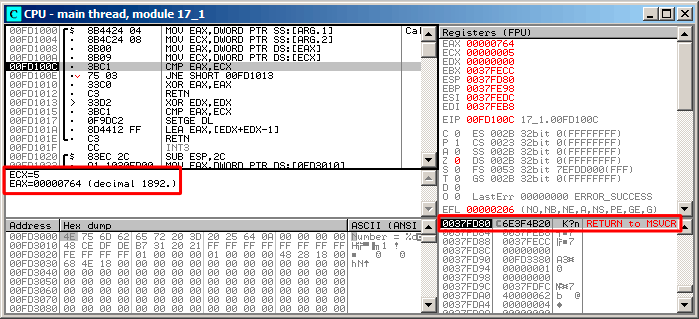
\includegraphics[scale=\FigScale]{patterns/18_pointers_to_functions/olly1.png}
\caption{\olly: \RU{первый вызов}\EN{first call of} \comp}
\label{fig:qsort_olly1}
\end{figure}

\RU{Для удобства, }\olly \RU{показывает сравниваемые значения в окне под окном кода}
\EN{shows the compared values in the window under the code window, for convenience}.
\RU{Мы можем так же увидеть, что}\EN{We can also see that the} \ac{SP} \RU{указывает на}\EN{points to} 
\ac{RA} \RU{где находится место в функции}\EN{, where the} 
\qsort \EN{function is }(\RU{на самом деле, находится в}\EN{located in} \TT{MSVCR100.DLL}).

\clearpage
\RU{Трассируя}\EN{By tracing} (F8) \RU{до инструкции}\EN{until the} \TT{RETN} 
\RU{и нажав F8 еще один раз, мы возвращаемся в функцию}\EN{instruction and pressing F8 one more time, 
we return to the} \qsort\EN{ function}:

\begin{figure}[H]
\centering
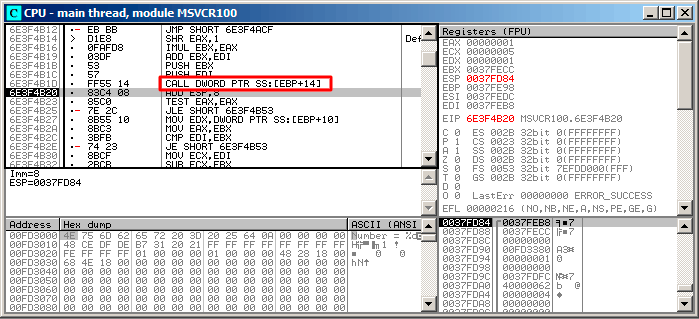
\includegraphics[scale=\FigScale]{patterns/18_pointers_to_functions/olly2.png}
\caption{\olly: \RU{код в}\EN{the code in} \qsort \RU{сразу после вызова}\EN{right after} \comp\EN{ call}}
\label{fig:qsort_olly2}
\end{figure}

\RU{Это был вызов функции сравнения}\EN{That was a call to the comparison function}.

\clearpage
\RU{Вот также скриншот момента второго вызова функции}\EN{Here is also a screenshot of the moment of the 
second call of} \comp\EMDASH{}\RU{теперь сравниваемые значения другие}
\EN{now values that have to be compared are different}:

\begin{figure}[H]
\centering
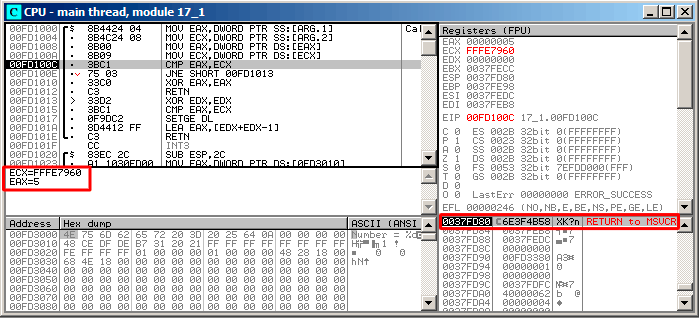
\includegraphics[scale=\FigScale]{patterns/18_pointers_to_functions/olly3.png}
\caption{\olly: \RU{второй вызов}\EN{second call of} \comp}
\label{fig:qsort_olly3}
\end{figure}

\fi

\subsection{MSVC + tracer}
\index{tracer}

\RU{Посмотрим, какие пары сравниваются}\EN{Let's also see which pairs are compared}.
\RU{Эти 10 чисел будут сортироваться}\EN{These 10 numbers are being sorted}: 
1892, 45, 200, -98, 4087, 5, -12345, 1087, 88, -100000.

\RU{Найдем адрес первой инструкции \CMP в \comp и это \TT{0x0040100C} и мы ставим точку останова на ней:}%
\EN{We got the address of the first \CMP instruction in \comp, it is \TT{0x0040100C} and we've set a breakpoint on it:}

\begin{lstlisting}
tracer.exe -l:17_1.exe bpx=17_1.exe!0x0040100C
\end{lstlisting}

\RU{Получаем информацию о регистрах на точке останова}%
\EN{Now we get some information about the registers at the breakpoint}:

\begin{lstlisting}
PID=4336|New process 17_1.exe
(0) 17_1.exe!0x40100c
EAX=0x00000764 EBX=0x0051f7c8 ECX=0x00000005 EDX=0x00000000
ESI=0x0051f7d8 EDI=0x0051f7b4 EBP=0x0051f794 ESP=0x0051f67c
EIP=0x0028100c
FLAGS=IF
(0) 17_1.exe!0x40100c
EAX=0x00000005 EBX=0x0051f7c8 ECX=0xfffe7960 EDX=0x00000000
ESI=0x0051f7d8 EDI=0x0051f7b4 EBP=0x0051f794 ESP=0x0051f67c
EIP=0x0028100c
FLAGS=PF ZF IF
(0) 17_1.exe!0x40100c
EAX=0x00000764 EBX=0x0051f7c8 ECX=0x00000005 EDX=0x00000000
ESI=0x0051f7d8 EDI=0x0051f7b4 EBP=0x0051f794 ESP=0x0051f67c
EIP=0x0028100c
FLAGS=CF PF ZF IF
...
\end{lstlisting}

\RU{Отфильтруем \TT{EAX} и \TT{ECX} и получим:}%
\EN{Let's filter out \TT{EAX} and \TT{ECX} and we got:}

\begin{lstlisting}
EAX=0x00000764 ECX=0x00000005
EAX=0x00000005 ECX=0xfffe7960
EAX=0x00000764 ECX=0x00000005
EAX=0x0000002d ECX=0x00000005
EAX=0x00000058 ECX=0x00000005
EAX=0x0000043f ECX=0x00000005
EAX=0xffffcfc7 ECX=0x00000005
EAX=0x000000c8 ECX=0x00000005
EAX=0xffffff9e ECX=0x00000005
EAX=0x00000ff7 ECX=0x00000005
EAX=0x00000ff7 ECX=0x00000005
EAX=0xffffff9e ECX=0x00000005
EAX=0xffffff9e ECX=0x00000005
EAX=0xffffcfc7 ECX=0xfffe7960
EAX=0x00000005 ECX=0xffffcfc7
EAX=0xffffff9e ECX=0x00000005
EAX=0xffffcfc7 ECX=0xfffe7960
EAX=0xffffff9e ECX=0xffffcfc7
EAX=0xffffcfc7 ECX=0xfffe7960
EAX=0x000000c8 ECX=0x00000ff7
EAX=0x0000002d ECX=0x00000ff7
EAX=0x0000043f ECX=0x00000ff7
EAX=0x00000058 ECX=0x00000ff7
EAX=0x00000764 ECX=0x00000ff7
EAX=0x000000c8 ECX=0x00000764
EAX=0x0000002d ECX=0x00000764
EAX=0x0000043f ECX=0x00000764
EAX=0x00000058 ECX=0x00000764
EAX=0x000000c8 ECX=0x00000058
EAX=0x0000002d ECX=0x000000c8
EAX=0x0000043f ECX=0x000000c8
EAX=0x000000c8 ECX=0x00000058
EAX=0x0000002d ECX=0x000000c8
EAX=0x0000002d ECX=0x00000058
\end{lstlisting}

\RU{Это}\EN{That's} 34 \RU{пары}\EN{pairs}.
\RU{Следовательно, алгоритму быстрой сортировки нужно 34 операции сравнения для сортировки этих
10-и чисел}\EN{Therefore, the quick sort algorithm needs 34 comparison operations to sort these 10 numbers}.

\clearpage
\subsection{MSVC + tracer (code coverage)}
\index{tracer}

\RU{Но можно также и воспользоваться возможностью tracer накапливать все возможные состояния регистров
и показать их в \IDA}\EN{We can also use the tracer's feature to collect all possible register values
and show them in \IDA}.

\RU{Трассируем все инструкции в функции \comp}\EN{Let's trace all instructions in \comp}:

\begin{lstlisting}
tracer.exe -l:17_1.exe bpf=17_1.exe!0x00401000,trace:cc
\end{lstlisting}

\RU{Получем .idc-скрипт для загрузки в \IDA и загружаем его}
\EN{We get an .idc-script for loading into \IDA and load it}:

\begin{figure}[H]
\centering
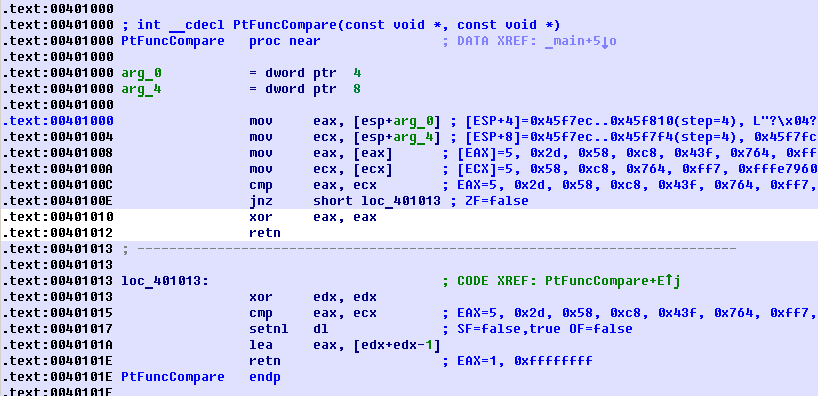
\includegraphics[scale=\FigScale]{patterns/18_pointers_to_functions/tracer_cc.png}
\caption{tracer \AndENRU IDA. N.B.: 
\RU{некоторые значения обрезаны справа}\EN{some values are cut at right}}
\label{fig:qsort_tracer_cc}
\end{figure}

\RU{Имя этой функции (PtFuncCompare) дала \IDA}\EN{\IDA gave the function a name (PtFuncCompare)}
\EMDASH{}\RU{видимо, потому что видит что указатель на эту функцию передается в \qsort}
\EN{because \IDA sees that the pointer to this function is passed to \qsort}.

\RU{Мы видим, что указатели $a$ и $b$ указывают на разные места внутри массива, 
но шаг между указателями --- 4, что логично, ведь в массиве хранятся 32-битные значения}
\EN{We see that the $a$ and $b$ pointers are pointing to various places in the array, but the step between
them is 4, as 32-bit values are stored in the array}.

\RU{Видно, что инструкции по адресам}\EN{We see that the instructions at} \TT{0x401010} \AndENRU 
\TT{0x401012} \RU{никогда не исполнялись}\EN{were never executed} 
(\RU{они и остались белыми}\EN{so they left as white}): 
\RU{действительно, функция}\EN{indeed,} \comp \RU{никогда не возвращала 0,
потому что в массиве нет одинаковых элементов}\EN{has never returned 0, because there no equal elements in the array}.

\ifdefined\IncludeGCC
\section{GCC}

\RU{Не слишком большая разница}\EN{Not a big difference}:

\begin{lstlisting}[caption=GCC]
                lea     eax, [esp+40h+var_28]
                mov     [esp+40h+var_40], eax
                mov     [esp+40h+var_28], 764h
                mov     [esp+40h+var_24], 2Dh
                mov     [esp+40h+var_20], 0C8h
                mov     [esp+40h+var_1C], 0FFFFFF9Eh
                mov     [esp+40h+var_18], 0FF7h
                mov     [esp+40h+var_14], 5
                mov     [esp+40h+var_10], 0FFFFCFC7h
                mov     [esp+40h+var_C], 43Fh
                mov     [esp+40h+var_8], 58h
                mov     [esp+40h+var_4], 0FFFE7960h
                mov     [esp+40h+var_34], offset comp
                mov     [esp+40h+var_38], 4
                mov     [esp+40h+var_3C], 0Ah
                call    _qsort
\end{lstlisting}

\RU{Функция \comp}\EN{\comp function}:

\begin{lstlisting}
                public comp
comp            proc near

arg_0           = dword ptr  8
arg_4           = dword ptr  0Ch

                push    ebp
                mov     ebp, esp
                mov     eax, [ebp+arg_4]
                mov     ecx, [ebp+arg_0]
                mov     edx, [eax]
                xor     eax, eax
                cmp     [ecx], edx
                jnz     short loc_8048458
                pop     ebp
                retn
loc_8048458:
                setnl   al
                movzx   eax, al
                lea     eax, [eax+eax-1]
                pop     ebp
                retn
comp            endp
\end{lstlisting}

\index{Linux!libc.so.6}
\RU{Реализация \qsort находится в \TT{libc.so.6}, и представляет собой просто wrapper
\footnote{понятие близкое к \gls{thunk function}} для \TT{qsort\_r()}.}
\EN{The implementation of \qsort is located in \TT{libc.so.6} and it is in fact just a wrapper
\footnote{a concept like \gls{thunk function}} for \TT{qsort\_r()}.}

\RU{Она, в свою очередь, вызывает \TT{quicksort()}, где есть вызовы определенной нами функции через 
переданный указатель:}
\EN{In turn, it is calling \TT{quicksort()}, where our defined function is called via a passed pointer:}

\begin{lstlisting}[caption=
(\RU{файл libc.so.6{,} версия glibc}\EN{file libc.so.6{,} glibc version}\EMDASH{}2.10.1)]

.text:0002DDF6                 mov     edx, [ebp+arg_10]
.text:0002DDF9                 mov     [esp+4], esi
.text:0002DDFD                 mov     [esp], edi
.text:0002DE00                 mov     [esp+8], edx
.text:0002DE04                 call    [ebp+arg_C]
...
\end{lstlisting}

\ifdefined\IncludeGDB
\subsection{GCC + GDB (\RU{с исходными кодами}\EN{with source code})}
\index{GDB}

\RU{Очевидно, у нас есть исходный код нашего примера на Си (\myref{qsort_c_src}), 
так что мы можем установить точку останова ($b$) на
номере строки}\EN{Obviously, we have the C-source code of our example (\myref{qsort_c_src}), 
so we can set a breakpoint ($b$) on line number}
(\RU{11-й --- это номер строки где происходит первое сравнение}\EN{11---the line where 
the first comparison occurs}).
\RU{Нам также нужно скомпилировать наш пример с ключом \TT{-g}, чтобы в исполняемом файле была
полная отладочная информация}\EN{We also need to compile the example with debugging information 
included (\TT{-g}), so the table
with addresses and corresponding line numbers is present}.
\RU{Мы можем так же выводить значения используя имена переменных}
\EN{We can also print values using variable names} (\TT{p}):
\RU{отладочная информация также содержит информацию о том, в каком регистре и/или элементе локального
стека находится какая переменная}\EN{the debugging information also has tells us which register and/or 
local stack element contains which variable}.

\index{Glibc}
\RU{Мы можем также увидеть стек}\EN{We can also see the stack} (\TT{bt}) 
\RU{и обнаружить что в Glibc используется какая-то вспомогательная функция с именем}
\EN{and find out that there is some intermediate function} 
\TT{msort\_with\_tmp()}\EN{ used in Glibc}.

\lstinputlisting[caption=GDB\RU{-сессия}\EN{ session}]{patterns/18_pointers_to_functions/GDB_source.txt}

\subsection{GCC + GDB (\RU{без исходных кодов}\EN{no source code})}
\index{GDB}

\RU{Но часто никаких исходных кодов нет вообще, так что мы можем дизассемблировать функцию \comp}
\EN{But often there is no source code at all, so we can disassemble the \comp function} (\TT{disas}), 
\RU{найти самую первую инструкцию \CMP и установить точку останова}\EN{find the very first
\CMP instruction and set a breakpoint} ($b$) \RU{по этому адресу}\EN{at that address}.
\RU{На каждой точке останова мы будем видеть содержимое регистров}
\EN{At each breakpoint, we are going to dump all register contents} (\TT{info registers}).
\RU{Информация из стека так же доступна}\EN{The stack information is also available} (\TT{bt}), 
\RU{но частичная: здесь нет номеров строк для функции \comp}
\EN{but partially: there is no line number information for \comp}.

\lstinputlisting[caption=GDB\RU{-сессия}\EN{ session}]{patterns/18_pointers_to_functions/GDB_no_source.txt}
\fi
\fi

\fi
\chapter{\RU{64-битные значения в 32-битной среде}\EN{64-bit values in 32-bit environment}}
\label{sec:64bit_in_32_env}

\ifx\LITE\undefined
\RU{В среде, где \ac{GPR}-ы 32-битные, 64-битные значения хранятся и передаются как пары 32-битных значений}
\EN{In a 32-bit environment, \ac{GPR}'s are 32-bit, so 64-bit values are stored and passed as 32-bit value pairs}
\footnote{\RU{Кстати, в 16-битной среде, 32-битные значения передаются 16-битными парами точно так же}
\EN{By the way, 32-bit values are passed as pairs in 16-bit environment in the same way}: 
\myref{win16_32bit_values}}.
\fi

\section{\RU{Возврат 64-битного значения}\EN{Returning of 64-bit value}}

\lstinputlisting{patterns/185_64bit_in_32_env/ret/0.c}

\subsection{x86}

\RU{64-битные значения в 32-битной среде возвращаются из функций в паре регистров \EDX{}:\EAX{}.}
\EN{In a 32-bit environment, 64-bit values are returned from functions in the \EDX{}:\EAX{} register pair.}

\lstinputlisting[caption=\Optimizing MSVC 2010]{patterns/185_64bit_in_32_env/ret/0_MSVC_2010_Ox.asm}

\ifdefined\IncludeARM
\subsection{ARM}

\RU{64-битное значение возвращается в паре регистров R0-R1 ---
(R1 это старшая часть и R0 --- младшая часть):}
\EN{A 64-bit value is returned in the R0-R1 register pair 
(R1 is for the high part and R0 for the low part):}

\lstinputlisting[caption=\OptimizingKeilVI (\ARMMode)]{patterns/185_64bit_in_32_env/ret/Keil_ARM_O3.s}

\fi

\ifdefined\IncludeMIPS
\subsection{MIPS}

\RU{64-битное значение возвращается в паре регистров V0-V1 (\$2-\$3) ---
(V0 (\$2) это старшая часть и V1 (\$3) --- младшая часть):}
\EN{A 64-bit value is returned in the V0-V1 (\$2-\$3) register pair 
(V0 (\$2) is for the high part and V1 (\$3) for the low part):}

\lstinputlisting[caption=\Optimizing GCC 4.4.5 (assembly listing)]{patterns/185_64bit_in_32_env/ret/0_MIPS.s}

\lstinputlisting[caption=\Optimizing GCC 4.4.5 (IDA)]{patterns/185_64bit_in_32_env/ret/0_MIPS_IDA.lst}
\fi

\section{\RU{Передача аргументов, сложение, вычитание}\EN{Arguments passing, addition, subtraction}}

\lstinputlisting{patterns/185_64bit_in_32_env/passing_add_sub/1.c}

\subsection{x86}

\lstinputlisting[caption=\Optimizing MSVC 2012 /Ob1]{patterns/185_64bit_in_32_env/passing_add_sub/1_MSVC.asm}

\RU{В}\EN{We can see in the} \TT{f\_add\_test()} \RU{видно, как каждое 64-битное число передается двумя 32-битными значениями,
сначала старшая часть, затем младшая}\EN{function that each 64-bit value is passed using two 32-bit values,
high part first, then low part}. \\
\\
\RU{Сложение и вычитание происходит также парами}\EN{Addition and subtraction occur in pairs as well}. \\
\\
\index{x86!\Instructions!ADC}
\RU{При сложении, в начале складываются младшие 32 бита}\EN{In addition, the low 32-bit part are added first}.
\RU{Если при сложении был перенос, выставляется флаг CF}\EN{If carry was occurred while adding, the CF flag is set}.
\RU{Следующая инструкция \TT{ADC} складывает старшие части чисел, но также прибавляет единицу если $CF=1$}
\EN{The following \TT{ADC} instruction adds the high parts of the values, and also adds 1 if $CF=1$}. \\
\\
\index{x86!\Instructions!SBB}
\RU{Вычитание также происходит парами}\EN{Subtraction also occurs in pairs}.
\RU{Первый}\EN{The first} \SUB \RU{может также включить флаг переноса CF, который затем будет проверяться в \TT{SBB}}
\EN{may also turn on the CF flag, which is to be checked in the subsequent \TT{SBB} instruction}:
\RU{если флаг переноса включен, то от результата отнимется единица}
\EN{if the carry flag is on, then 1 is also to be subtracted from the result}. \\
\\
\RU{Легко увидеть, как результат работы \TT{f\_add()} затем передается в \printf{}}\EN{It is easy to see how
the \TT{f\_add()} function result is then passed to \printf{}}.

\ifdefined\IncludeGCC
\lstinputlisting[caption=GCC 4.8.1 -O1 -fno-inline]{patterns/185_64bit_in_32_env/passing_add_sub/1_GCC.asm}

\RU{Код GCC почти такой же}\EN{GCC code is the same}.
\fi

\ifdefined\IncludeARM
\subsection{ARM}

\lstinputlisting[caption=\OptimizingKeilVI (\ARMMode)]{patterns/185_64bit_in_32_env/passing_add_sub/Keil_ARM_O3.s}

\index{ARM!\Instructions!ADDS}
\index{ARM!\Instructions!SUBS}
\index{ARM!\Instructions!ADC}
\index{ARM!\Instructions!SBC}
\RU{Первое 64-битное значение передается в паре регистров R0 и R1, второе --- в паре R2 и R3.}
\EN{The first 64-bit value is passed in R0 and R1 register pair, the second in R2 and R3 register pair.}
\RU{В ARM также есть инструкция ADC (учитывающая флаг переноса) и SBC (\q{subtract with carry} --- вычесть
с переносом).}
\EN{ARM has the ADC instruction as well (which counts carry flag) and SBC (\q{subtract with carry}).}

\RU{Важная вещь: когда младшие части слагаются/вычитаются, используются инструкции ADDS и SUBS с суффиксом
-S.}
\EN{Important thing: when the low parts are added/subtracted, ADDS and SUBS instructions with -S suffix are used.}
\RU{Суффикс -S означает \q{set flags} (установить флаги), а флаги (особенно флаг переноса) это то что однозначно
нужно последующим инструкциями ADC/SBC.}
\EN{The -S suffix stands for \q{set flags}, and flags (esp. carry flag) is what consequent ADC/SBC instructions
definitely need.}

\RU{А иначе инструкции без суффикса -S здесь вполне бы подошли (ADD и SUB).}
\EN{Otherwise, instructions without the -S suffix would do the job (ADD and SUB).}

\fi

\ifdefined\IncludeMIPS
\subsection{MIPS}

\lstinputlisting[caption=\Optimizing GCC 4.4.5 (IDA)]{patterns/185_64bit_in_32_env/passing_add_sub/MIPS_O3_IDA.lst.\LANG}

\RU{В MIPS нет регистра флагов, так что эта информация не присутствует после исполнения арифметических операций.}
\EN{MIPS has no flags register, so there is no such information present after the execution of arithmetic operations.}
\EN{So there are no instructions like x86's ADC and SBB.}
\RU{Так что здесь нет инструкций как ADC или SBB в x86.}
\RU{Чтобы получить информацию о том, был бы выставлен флаг переноса, происходит сравнение (используя инструкцию
\q{SLTU}), которая выставляет целевой регистр в 1 или 0.}
\EN{To know if the carry flag would be set, a comparison (using \q{SLTU} instruction) also occurs, 
which sets the destination register to 1 or 0.}
\RU{Эта 1 или 0 затем прибавляется к итоговому результату, или вычитается.}
\EN{This 1 or 0 is then added or subtracted to/from the final result.}

\fi

\section{\RU{Умножение, деление}\EN{Multiplication, division}}

\lstinputlisting{patterns/185_64bit_in_32_env/multdiv/2.c}

\subsection{x86}

\lstinputlisting[caption=\Optimizing MSVC 2013 /Ob1]{patterns/185_64bit_in_32_env/multdiv/2_MSVC.asm.\LANG}

\RU{Умножение и деление --- это более сложная операция, так что обычно, компилятор встраивает вызовы библиотечных функций,
делающих это}\EN{Multiplication and division are more complex operations, so usually the compiler embeds calls to
a library functions doing that}.

\ifx\LITE\undefined
\RU{Значение этих библиотечных функций, здесь}\EN{These functions are described here}: \myref{sec:MSVC_library_func}.
\fi

\ifdefined\IncludeGCC
\lstinputlisting[caption=\Optimizing GCC 4.8.1 -fno-inline]{patterns/185_64bit_in_32_env/multdiv/2_GCC.asm.\LANG}

\RU{GCC делает почти то же самое, тем не менее,
встраивает код умножения прямо в функцию, посчитав что так будет эффективнее}\EN{GCC does the expected, but the multiplication
code is inlined right in the function, thinking it could be more efficient}.
\RU{У GCC другие имена библиотечных функций}\EN{GCC has different library function names}: \myref{sec:GCC_library_func}.
\fi

\ifdefined\IncludeARM
\subsection{ARM}

\RU{Keil для режима Thumb вставляет вызовы библиотечных функций:}
\EN{Keil for Thumb mode inserts library subroutine calls:}

\lstinputlisting[caption=\OptimizingKeilVI (\ThumbMode)]{patterns/185_64bit_in_32_env/multdiv/Keil_thumb_O3.s}

\RU{Keil для режима ARM, тем не менее, может сгенерировать код для умножения 64-битных чисел:}
\EN{Keil for ARM mode, on the other hand, is able to produce 64-bit multiplication code:}

\lstinputlisting[caption=\OptimizingKeilVI (\ARMMode)]{patterns/185_64bit_in_32_env/multdiv/Keil_ARM_O3.s}
% TODO add explanation
\fi

\ifdefined\IncludeMIPS
\subsection{MIPS}

\Optimizing GCC \ForENRU MIPS 
\EN{can generate 64-bit multiplication code, but has to call a library routine for 64-bit division:}
\RU{может генерировать код для 64-битного умножения, но для 64-битного деления приходится вызывать библиотечную функцию:}

\lstinputlisting[caption=\Optimizing GCC 4.4.5 (IDA)]{patterns/185_64bit_in_32_env/multdiv/MIPS_O3_IDA.lst}

\RU{Тут также много \ac{NOP}-ов, это возможно заполнение delay slot-ов после инструкции умножения (она ведь работает
медленнее прочих инструкций).}
\EN{There are a lot of \ac{NOP}s, probably delay slots filled after the multiplication instruction (it's slower
than other instructions, after all).}

% TODO add explanation
\fi

\section{\RU{Сдвиг вправо}\EN{Shifting right}}

\lstinputlisting{patterns/185_64bit_in_32_env/shifting/3.c}

\subsection{x86}

\lstinputlisting[caption=\Optimizing MSVC 2012 /Ob1]{patterns/185_64bit_in_32_env/shifting/3_MSVC.asm}

\ifdefined\IncludeGCC
\lstinputlisting[caption=\Optimizing GCC 4.8.1 -fno-inline]{patterns/185_64bit_in_32_env/shifting/3_GCC.asm}
\fi

\index{x86!\Instructions!SHRD}
\RU{Сдвиг происходит также в две операции: в начале сдвигается младшая часть, затем старшая}
\EN{Shifting also occurs in two passes: first the lower part is shifted, then the higher part}.
\RU{Но младшая часть сдвигается
при помощи инструкции \TT{SHRD}, она сдвигает значение в \EDX{} на 7 бит, но подтягивает новые биты из \EAX{}, т.е. из старшей части.}
\EN{But the lower part is shifted with the help of the \TT{SHRD} instruction, it shifts the value of \EDX{} by 7 bits, but pulls new bits
from \EAX{}, i.e., from the higher part.}
\RU{Старшая часть сдвигается более известной инструкцией \SHR{}: действительно, ведь освободившиеся биты в старшей части нужно
просто заполнить нулями}\EN{The higher part is shifted using the more popular \SHR{} instruction: indeed, the freed bits in the higher part
must be filled with zeroes}.

\ifdefined\IncludeARM
\subsection{ARM}

\RU{В ARM нет такой инструкции как SHRD в x86, так что компилятору Keil приходится всё это делать,
используя простые сдвиги и операции \q{ИЛИ}:}
\EN{ARM doesn't have such instruction as SHRD in x86, so the Keil compiler ought to do this using simple shifts
and OR operations:}

\lstinputlisting[caption=\OptimizingKeilVI (\ARMMode)]{patterns/185_64bit_in_32_env/shifting/Keil_ARM_O3.s}

\lstinputlisting[caption=\OptimizingKeilVI (\ThumbMode)]{patterns/185_64bit_in_32_env/shifting/Keil_thumb_O3.s}
% TODO add explanation
\fi

\ifdefined\IncludeMIPS
\subsection{MIPS}

\ifdefined\IncludeGCC
\EN{GCC for MIPS follows the same algorithm as Keil does for Thumb mode:}
\RU{GCC для MIPS реализует тот же алгоритм, что сделал Keil для режима Thumb:}

\lstinputlisting[caption=\Optimizing GCC 4.4.5 (IDA)]{patterns/185_64bit_in_32_env/shifting/MIPS_O3_IDA.lst}
\fi

% TODO add explanation
\fi

\section{\RU{Конвертирование 32-битного значения в 64-битное}\EN{Converting 32-bit value into 64-bit one}}
\label{subsec:sign_extending_32_to_64}

\lstinputlisting{patterns/185_64bit_in_32_env/conversion/4.c}

\subsection{x86}

\lstinputlisting[caption=\Optimizing MSVC 2012]{patterns/185_64bit_in_32_env/conversion/MSVC2012_Ox.asm}

\RU{Здесь появляется необходимость расширить 32-битное знаковое значение в 64-битное знаковое.}
\EN{Here we also run into necessity to extend a 32-bit signed value into a 64-bit signed one.}
\RU{Конвертировать беззнаковые значения очень просто: нужно просто выставить в 0 все биты в старшей части}
\EN{Unsigned values are converted straightforwardly: all bits in the higher part must be set to 0}.
\RU{Но для знаковых типов это не подходит: знак числа должен быть скопирован в старшую часть числа-результата}
\EN{But this is not appropriate for signed data types: the sign has to be copied into the higher part of the resulting number}.
\index{x86!\Instructions!CDQ}
\RU{Здесь это делает инструкция \TT{CDQ}, она берет входное значение в \EAX{}, расширяет его до 64-битного,
и оставляет его в паре регистров \EDX{}:\EAX{}}
\EN{The \TT{CDQ} instruction does that here, it takes its input value in \EAX{}, extends it to 64-bit and leaves it
in the \EDX{}:\EAX{} register pair}.
\RU{Иными словами, инструкция \TT{CDQ} узнает знак числа в \EAX{} (просто берет самый старший бит в \EAX{}) и в зависимости от этого,
выставляет все 32 бита в \EDX{} в 0 или в 1}\EN{In other words, \TT{CDQ} gets the number sign from \EAX{} (by getting the
most significant bit in \EAX{}), and depending of it, sets all 32 bits in \EDX{} to 0 or 1}.
\RU{Её работа в каком-то смысле напоминает работу инструкции \MOVSX{}}\EN{Its operation is somewhat
similar to the \MOVSX{} instruction}.

\ifdefined\IncludeARM
\subsection{ARM}

\lstinputlisting[caption=\OptimizingKeilVI (\ARMMode)]{patterns/185_64bit_in_32_env/conversion/Keil_ARM_O3.s}

\RU{Keil для ARM работает иначе: он просто сдвигает (арифметически) входное значение на 31 бит вправо.}
\EN{Keil for ARM is different: it just arithmetically shifts right the input value by 31 bits.}
\RU{Как мы знаем, бит знака это \ac{MSB}, и арифметический сдвиг копирует бит знака в \q{появляющихся} битах.}
\EN{As we know, the sign bit is \ac{MSB}, and the arithmetical shift copies the sign bit into the \q{emerged} bits.}
\RU{Так что после инструкции \q{ASR r1,r0,\#31}, R1 будет содержать 0xFFFFFFFF если входное значение
было отрицательным, или 0 в противном случае.}
\EN{So after \q{ASR r1,r0,\#31}, R1 containing 0xFFFFFFFF if the input value was negative
and 0 otherwise.}
\RU{R1 содержит старшую часть возвращаемого 64-битного значения.}
\EN{R1 contains the high part of the resulting 64-bit value.}

\RU{Другими словами, этот код просто копирует \ac{MSB} (бит знака) из входного значения в R0 во все
биты старшей 32-битной части итогового 64-битного значения.}
\EN{In other words, this code just copies the \ac{MSB} (sign bit) from the input value in R0 to all bits
of the high 32-bit part of the resulting 64-bit value.}

\fi

\ifdefined\IncludeMIPS
\subsection{MIPS}

\ifdefined\IncludeGCC
\EN{GCC for MIPS does the same as Keil did for ARM mode:}
\RU{GCC для MIPS делает то же, что сделал Keil для режима ARM:}

\lstinputlisting[caption=\Optimizing GCC 4.4.5 (IDA)]{patterns/185_64bit_in_32_env/conversion/MIPS_O3_IDA.lst}
\fi

\fi


\ifx\LITE\undefined
\chapter{SIMD}

\label{SIMD_x86}
\ac{SIMD} \RU{это акроним}\EN{is an acronym}: \IT{Single Instruction, Multiple Data}.

\RU{Как можно судить по названию, это обработка множества данных исполняя только одну инструкцию.}
\EN{As its name implies, it processes multiple data using only one instruction.}

\RU{Как и \ac{FPU}, эта подсистема процессора выглядит так же отдельным процессором внутри x86.}
\EN{Like the \ac{FPU}, that \ac{CPU} subsystem looks like a separate processor inside x86.}

\index{x86!MMX}
\RU{SIMD в x86 начался с MMX. Появилось 8 64-битных регистров MM0-MM7.}
\EN{SIMD began as MMX in x86. 8 new 64-bit registers appeared: MM0-MM7.}

\RU{Каждый MMX-регистр может содержать 2 32-битных значения, 4 16-битных или же 8 байт. 
Например, складывая значения двух MMX-регистров, можно складывать одновременно 8 8-битных значений.}
\EN{Each MMX register can hold 2 32-bit values, 4 16-bit values or 8 bytes.
For example, it is possible to add 8 8-bit values (bytes) simultaneously by adding two values in MMX registers.}

\RU{Простой пример, это некий графический редактор, который хранит открытое изображение как двумерный массив. 
Когда пользователь меняет яркость изображения, редактору нужно, например, прибавить некий коэффициент 
ко всем пикселям, или отнять. 
Для простоты можно представить, что изображение у нас бело-серо-черное и каждый пиксель занимает один байт, 
то с помощью MMX можно менять яркость сразу у восьми пикселей.}
\EN{One simple example is a graphics editor that represents an image as a two dimensional array.
When the user changes the brightness of the image, the editor must add or subtract a coefficient to/from each pixel value.
For the sake of brevity if we say that the image is grayscale and each pixel is defined by one 8-bit byte, then it is possible
to change the brightness of 8 pixels simultaneously.}
\RU{Кстати, вот причина почему в SIMD присутствуют инструкции с \IT{насыщением} (\IT{saturation}).}
\EN{By the way, this is the reason why the \IT{saturation} instructions are present in SIMD.}
\RU{Когда пользователь в графическом редакторе изменяет яркость, переполнение и антипереполнение (\IT{underflow})
не нужны, так что в SIMD имеются, например, инструкции сложения, которые ничего не будут прибавлять
если максимальное значение уже достигнуто,\etc{}.}
\EN{When the user changes the brightness in the graphics editor, overflow and underflow are not desirable, 
so there are addition instructions in SIMD which are not adding anything if the maximum value is reached, \etc{}.}

\RU{Когда MMX только появилось, эти регистры на самом деле располагались в FPU-регистрах. 
Можно было использовать 
либо FPU либо MMX в одно и то же время. Можно подумать, что Intel решило немного сэкономить на транзисторах, 
но на самом деле причина такого симбиоза проще ~--- более старая \ac{OS} не знающая о дополнительных 
регистрах процессора не будет сохранять их во время переключения задач, а вот регистры FPU сохранять будет. 
Таким образом, процессор с MMX + старая \ac{OS} + задача, использующая возможности MMX = все 
это может работать вместе.}
\EN{When MMX appeared, these registers were actually located in the FPU's registers. 
It was possible to use either FPU or MMX at the same time. One might think that Intel saved on transistors,
but in fact the reason of such symbiosis was simpler~---older \ac{OS}es that are not aware 
of the additional CPU registers would not save them at the context switch, 
but saving the FPU registers.
Thus, MMX-enabled CPU + old \ac{OS} + process utilizing MMX features will still work.}

\index{x86!SSE}
\index{x86!SSE2}
SSE\EMDASH\RU{это расширение регистров до 128 бит, теперь уже отдельно от FPU.}\EN{is extension of the SIMD registers to 128 bits, now separate from the FPU.}

\index{x86!AVX}
AVX\EMDASH\RU{расширение регистров до 256 бит.}\EN{another extension, to 256 bits.}

\RU{Немного о практическом применении.}\EN{Now about practical usage.}

\RU{Конечно же, это копирование блоков в памяти (\TT{memcpy}), сравнение (\TT{memcmp}), и подобное.}
\EN{Of course, this is memory copy routines (\TT{memcpy}), memory comparing (\TT{memcmp}) and so on.}

\index{DES}
\RU{Еще пример: имеется алгоритм шифрования DES, который берет 64-битный блок, 56-битный ключ, 
шифрует блок с ключом и образуется 64-битный результат.
Алгоритм DES можно легко представить в виде очень большой электронной цифровой схемы, 
с проводами, элементами И, ИЛИ, НЕ.}
\EN{One more example: the DES encryption algorithm takes a 64-bit block and a 56-bit key, encrypt the block and produces a 64-bit result.
The DES algorithm may be considered as a very large electronic circuit, with wires and AND/OR/NOT gates.}

\label{bitslicedes}
\newcommand{\URLBS}{\url{http://go.yurichev.com/17329}}

\RU{Идея bitslice DES\footnote{\URLBS} ~--- это обработка сразу группы блоков и ключей одновременно. 
Скажем, на x86 переменная типа \IT{unsigned int} вмещает в себе 32 бита, так что там можно хранить 
промежуточные результаты сразу для 32-х блоков-ключей, используя 64+56 переменных типа \IT{unsigned int}.}
\EN{Bitslice DES\footnote{\URLBS}~---is the idea of processing groups of blocks and keys simultaneously.
Let's say, variable of type \IT{unsigned int} on x86 can hold up to 32 bits, so it is possible to store there
intermediate results for 32 block-key pairs simultaneously, using 64+56 variables of type \IT{unsigned int}.}

\index{\oracle}
\RU{Существует утилита для перебора паролей/хешей \oracle (которые основаны на алгоритме DES), 
реализующая алгоритм bitslice DES для SSE2 и AVX\EMDASH{}и теперь возможно шифровать одновременно 
128 или 256 блоков-ключей:}%
\EN{There is an utility to brute-force \oracle passwords/hashes (ones based on DES),
using slightly modified bitslice DES algorithm for SSE2 and AVX\EMDASH{}now it is possible to encrypt 128 
or 256 block-keys pairs simultaneously.}

\url{http://go.yurichev.com/17313}

% sections
\section{\RU{Векторизация}\EN{Vectorization}}

\newcommand{\URLVEC}{\href{http://go.yurichev.com/17080}{Wikipedia: vectorization}}

\RU{Векторизация\footnote{\URLVEC} это когда у вас есть цикл, который берет на вход несколько массивов и выдает, 
например, один массив данных. 
Тело цикла берет некоторые элементы из входных массивов, что-то делает с ними и помещает в выходной. 
%Важно, что операция, применяемая ко всем элементам одна и та же. 
Векторизация ~--- это обрабатывать несколько элементов одновременно.}
\EN{Vectorization\footnote{\URLVEC} is when, for example, you have a loop taking couple of arrays for input and producing one array.
The loop body takes values from the input arrays, does something and puts the result into the output array.
%It is important that there is only a single operation applied to each element.
Vectorization is to process several elements simultaneously.}

\RU{Векторизация ~--- это не самая новая технология: автор сих строк видел её по крайней мере на 
линейке суперкомпьютеров Cray Y-MP от 1988, когда работал на его версии-\q{лайт} Cray Y-MP EL
\footnote{Удаленно. Он находится в музее суперкомпьютеров: \url{http://go.yurichev.com/17081}}}
\EN{Vectorization is not very fresh technology: the author of this textbook saw it at least on the Cray Y-MP 
supercomputer line from 1988 when he played with its \q{lite} version Cray Y-MP EL
\footnote{Remotely. It is installed in the museum of supercomputers: \url{http://go.yurichev.com/17081}}}.

% FIXME! add assembly listing!
\RU{Например:}\EN{For example:}

\begin{lstlisting}
for (i = 0; i < 1024; i++)
{
    C[i] = A[i]*B[i];
}
\end{lstlisting}

\RU{Этот фрагмент кода берет элементы из A и B, перемножает и сохраняет результат в C.}
\EN{This fragment of code takes elements from A and B, multiplies them and saves the result into C.}

\index{x86!\Instructions!PLMULLD}
\index{x86!\Instructions!PLMULHW}
\newcommand{\PMULLD}{\IT{PMULLD} (\IT{\RU{Перемножить запакованные знаковые DWORD и сохранить младшую часть результата}
\EN{Multiply Packed Signed Dword Integers and Store Low Result}})}
\newcommand{\PMULHW}{\TT{PMULHW} (\IT{\RU{Перемножить запакованные знаковые DWORD и сохранить старшую часть результата}
\EN{Multiply Packed Signed Integers and Store High Result}})}

\RU{Если представить, что каждый элемент массива ~--- это 32-битный \Tint, то их можно загружать сразу 
по 4 из А в 128-битный XMM-регистр, 
из B в другой XMM-регистр и выполнив инструкцию \PMULLD{} и \PMULHW{}, можно получить 4 64-битных 
\glslink{product}{произведения} сразу.}
\EN{If each array element we have is 32-bit \Tint, then it is possible to load 4 elements from A into a 128-bit 
XMM-register, from B to another XMM-registers, and by executing \PMULLD{} and \PMULHW{}, 
it is possible to get 4 64-bit \glspl{product} at once.}

\RU{Таким образом, тело цикла исполняется $1024/4$ раза вместо 1024, что в 4 раза меньше, и, конечно, быстрее.}
\EN{Thus, loop body execution count is $1024/4$ instead of 1024, that is 4 times less and, of course, faster.}

\newcommand{\URLINTELVEC}{\href{http://go.yurichev.com/17082}{Excerpt: Effective Automatic Vectorization}}

\subsection{\RU{Пример сложения}\EN{Addition example}}

\index{Intel C++}
\RU{Некоторые компиляторы умеют делать автоматическую векторизацию в простых случаях, 
например, Intel C++\footnote{Еще о том, как Intel C++ умеет автоматически векторизовать циклы: \URLINTELVEC}.}
\EN{Some compilers can do vectorization automatically in simple cases, 
e.g., Intel C++\footnote{More about Intel C++ automatic vectorization: \URLINTELVEC}.}

\RU{Вот очень простая функция:}\EN{Here is tiny function:}

\begin{lstlisting}
int f (int sz, int *ar1, int *ar2, int *ar3)
{
	for (int i=0; i<sz; i++)
		ar3[i]=ar1[i]+ar2[i];

	return 0;
};
\end{lstlisting}

\subsubsection{Intel C++}

\RU{Компилируем её при помощи}\EN{Let's compile it with} Intel C++ 11.1.051 win32:

\begin{verbatim}
icl intel.cpp /QaxSSE2 /Faintel.asm /Ox
\end{verbatim}

\RU{Имеем такое (в \IDA):}\EN{We got (in \IDA):}

\lstinputlisting{patterns/19_SIMD/18_1.asm.\LANG}

\RU{Инструкции, имеющие отношение к SSE2 это:}\EN{The SSE2-related instructions are:}
\index{x86!\Instructions!MOVDQA}
\index{x86!\Instructions!MOVDQU}
\index{x86!\Instructions!PADDD}
\begin{itemize}
\item
\MOVDQU (\IT{Move Unaligned Double Quadword})\EMDASH\RU{она просто загружает 16 байт из памяти в XMM-регистр}
\EN{just loads 16 bytes from memory into a XMM-register}.

\item
\PADDD (\IT{Add Packed Integers})\EMDASH\RU{складывает сразу 4 пары 32-битных чисел и оставляет в первом операнде результат. 
Кстати, если произойдет переполнение, то исключения не произойдет и никакие флаги не установятся, 
запишутся просто младшие 32 бита результата. 
Если один из операндов \PADDD ~--- адрес значения в памяти, 
то требуется чтобы адрес был выровнен по 16-байтной границе. Если он не выровнен, произойдет исключение
\footnote{О выравнивании данных см. также: \URLWPDA}.}
\EN{adds 4 pairs of 32-bit numbers and leaves the result in the first operand.
By the way, no exception is raised in case of overflow and no flags are to be set, 
just the low 32 bits of the result are to be stored.
If one of \PADDD's operands is the address of a value in memory,
then the address must be aligned on a 16-byte boundary. 
If it is not aligned, an exception will be triggered
\footnote{More about data alignment: \URLWPDA}.}

\item
\MOVDQA (\IT{Move Aligned Double Quadword})\RU{\EMDASH тоже что и \MOVDQU, только подразумевает 
что адрес в памяти выровнен по 16-байтной границе. 
Если он не выровнен, произойдет исключение. 
\MOVDQA работает быстрее чем \MOVDQU, но требует вышеозначенного.}
\EN{is the same as \MOVDQU, but requires the address of the value in memory to be aligned on a 16-bit boundary.
If it is not aligned, exception will be raised.
\MOVDQA works faster than \MOVDQU, but requires aforesaid.}

\end{itemize}

\RU{Итак, эти SSE2-инструкции исполнятся только в том случае если еще осталось просуммировать 
4 пары переменных типа \Tint плюс если указатель \TT{ar3} выровнен по 16-байтной границе.}
\EN{So, these SSE2-instructions are to be executed only in case there are more than 4 pairs to work on
and the pointer \TT{ar3} is aligned on a 16-byte boundary.}

\RU{Более того, если еще и \TT{ar2} выровнен по 16-байтной границе, 
то будет выполняться этот фрагмент кода:}
\EN{Also, if \TT{ar2} is aligned on a 16-byte boundary as well, 
this fragment of code is to be executed:}

\begin{lstlisting}
movdqu  xmm0, xmmword ptr [ebx+edi*4] ; ar1+i*4
paddd   xmm0, xmmword ptr [esi+edi*4] ; ar2+i*4
movdqa  xmmword ptr [eax+edi*4], xmm0 ; ar3+i*4
\end{lstlisting}

\RU{А иначе, значение из \TT{ar2} загрузится в \XMM{0} используя инструкцию \MOVDQU, 
которая не требует выровненного указателя, зато может работать чуть медленнее:}
\EN{Otherwise, the value from \TT{ar2} is to be loaded into \XMM{0} using \MOVDQU,
which does not require aligned pointer, but may work slower:}

\lstinputlisting{patterns/19_SIMD/18_1_excerpt.asm.\LANG}

\RU{А во всех остальных случаях, будет исполняться код, который был бы, как если бы не была 
включена поддержка SSE2.}
\EN{In all other cases, non-SSE2 code is to be executed.}

\ifdefined\IncludeGCC
\subsubsection{GCC}

\newcommand{\URLGCCVEC}{\url{http://go.yurichev.com/17083}}

\RU{Но и GCC умеет кое-что векторизировать\footnote{Подробнее о векторизации в GCC: \URLGCCVEC}, 
если компилировать с опциями \Othree и включить поддержку SSE2: \TT{-msse2}.}
\EN{GCC may also vectorize in simple cases\footnote{More about GCC vectorization support: \URLGCCVEC},
if the \Othree option is used and SSE2 support is turned on: \TT{-msse2}.}

\RU{Вот что вышло}\EN{What we get} (GCC 4.4.1):

\lstinputlisting{patterns/19_SIMD/18_2_gcc_O3.asm}

\RU{Почти то же самое, хотя и не так дотошно, как Intel C++.}
\EN{Almost the same, however, not as meticulously as Intel C++.}

\subsection{\RU{Пример копирования блоков}\EN{Memory copy example}}
\label{vec_memcpy}

\RU{Вернемся к простому примеру memcpy()}\EN{Let's revisit the simple memcpy() example}
(\myref{loop_memcpy}):

\lstinputlisting{memcpy.c}

\RU{И вот что делает оптимизирующий GCC 4.9.1:}
\EN{And that's what optimizations GCC 4.9.1 did:}

\lstinputlisting[caption=\Optimizing GCC 4.9.1 x64]{patterns/19_SIMD/memcpy_GCC49_x64_O3.s.\LANG}
\fi

\section{\RU{Реализация \strlen при помощи SIMD}\EN{SIMD \strlen implementation}}
\label{SIMD_strlen}

\newcommand{\URLMSDNSSE}{\href{http://go.yurichev.com/17262}{MSDN: MMX, SSE, and SSE2 Intrinsics}}

\RU{Прежде всего, следует заметить, что SIMD-инструкции можно вставлять в \CCpp код при помощи специальных 
макросов\footnote{\URLMSDNSSE}. В MSVC, часть находится в файле \TT{intrin.h}.}
\EN{It has to be noted that the \ac{SIMD} instructions can be inserted in \CCpp code via 
special macros\footnote{\URLMSDNSSE}.
For MSVC, some of them are located in the \TT{intrin.h} file.}

\newcommand{\URLSTRLEN}{http://go.yurichev.com/17330}

\index{\CStandardLibrary!strlen()}
\RU{Имеется возможность реализовать функцию \strlen\footnote{strlen() ~--- стандартная функция Си 
для подсчета длины строки} при помощи SIMD-инструкций, работающий в 2-2.5 раза быстрее обычной реализации. 
Эта функция будет загружать в XMM-регистр сразу 16 байт и проверять каждый на ноль}
\EN{It is possible to implement the \strlen function\footnote{strlen()~---standard C library function for calculating
string length} using SIMD instructions that works 2-2.5 times faster than the common implementation.
This function loads 16 characters into a XMM-register and check each against zero}
\footnote{\RU{Пример базируется на исходнике отсюда: \url{\URLSTRLEN}.}
\EN{The example is based on source code from: \url{\URLSTRLEN}.}}.

\lstinputlisting{patterns/19_SIMD/18_3.c}

\RU{Компилируем в MSVC 2010 с опцией \Ox:}\EN{Let's compile it in MSVC 2010 with \Ox option:}

\lstinputlisting[caption=\Optimizing MSVC 2010]{patterns/19_SIMD/18_4_msvc_Ox.asm.\LANG}

\RU{Итак, прежде всего, мы проверяем указатель \TT{str}, выровнен ли он по 16-байтной границе. 
Если нет, то мы вызовем обычную реализацию \strlen.}
\EN{First, we check if the \TT{str} pointer is aligned on a 16-byte boundary.
If not, we call the generic \strlen implementation.}

\RU{Далее мы загружаем по 16 байт в регистр \XMM{1} при помощи команды \MOVDQA.}
\EN{Then, we load the next 16 bytes into the \XMM{1} register using \MOVDQA.}

\RU{Наблюдательный читатель может спросить, почему в этом месте мы не можем использовать \MOVDQU, 
которая может загружать откуда угодно не взирая на факт, выровнен ли указатель?}
\EN{An observant reader might ask, why can't \MOVDQU be used here since it can load data from the memory
regardless pointer alignment?}

\RU{Да, можно было бы сделать вот как: если указатель выровнен, загружаем используя \MOVDQA, 
иначе используем работающую чуть медленнее \MOVDQU.}
\EN{Yes, it might be done in this way: if the pointer is aligned, load data using \MOVDQA,
if not~---use the slower \MOVDQU.}

\RU{Однако здесь кроется не сразу заметная проблема, которая проявляется вот в чем:}
\EN{But here we are may hit another caveat:}

\index{Page (memory)}
\newcommand{\URLPAGE}{\href{http://go.yurichev.com/17136}{wikipedia}}

\RU{В \ac{OS} линии \gls{Windows NT} (и не только), память выделяется страницами по 4 KiB (4096 байт). 
Каждый win32-процесс якобы имеет в наличии 4 GiB, но на самом деле, 
только некоторые части этого адресного пространства присоединены к реальной физической памяти. 
Если процесс обратится к блоку памяти, которого не существует, сработает исключение. 
Так работает \ac{VM}\footnote{\URLPAGE}.}
\EN{In the \gls{Windows NT} line of \ac{OS} (but not limited to it), memory is allocated by pages of 4 KiB (4096 bytes).
Each win32-process has 4 GiB available, but in fact, only some parts
of the address space are connected to real physical memory.
If the process is accessing an absent memory block, an exception is to be raised.
That's how \ac{VM} works\footnote{\URLPAGE}.}

\RU{Так вот, функция, читающая сразу по 16 байт, имеет возможность нечаянно вылезти за границу 
выделенного блока памяти. 
Предположим, \ac{OS} выделила программе 8192 (0x2000) байт по адресу 0x008c0000. 
Таким образом, блок занимает байты с адреса 0x008c0000 по 0x008c1fff включительно.}
\EN{So, a function loading 16 bytes at once  may step over the border of an allocated memory block.
Let's say that the \ac{OS} has allocated 8192 (0x2000) bytes at address 0x008c0000.
Thus, the block is the bytes starting from address 0x008c0000 to 0x008c1fff inclusive.}

\RU{За этим блоком, то есть начиная с адреса 0x008c2000 нет вообще ничего, т.е. \ac{OS} не выделяла там память. 
Обращение к памяти начиная с этого адреса вызовет исключение.}
\EN{After the block, that is, starting from address 0x008c2000 there is nothing at all, e.g. the \ac{OS} not allocated
any memory there.
Any attempt to access memory starting from that address will raise an exception.}

\RU{И предположим, что программа хранит некую строку из, скажем, пяти символов почти в самом конце блока, 
что не является преступлением:}
\EN{And let's consider the example in which the program is holding a string that contains 5 characters almost at the end of a block,
and that is not a crime.}

\begin{center}
  \begin{tabular}{ | l | l | }
    \hline
        0x008c1ff8 & 'h' \\
        0x008c1ff9 & 'e' \\
        0x008c1ffa & 'l' \\
        0x008c1ffb & 'l' \\
        0x008c1ffc & 'o' \\
        0x008c1ffd & '\textbackslash{}x00' \\
        0x008c1ffe & \RU{здесь случайный мусор}\EN{random noise} \\
        0x008c1fff & \RU{здесь случайный мусор}\EN{random noise} \\
    \hline
  \end{tabular}
\end{center}

\RU{В обычных условиях, программа вызывает \strlen передав ей указатель на строку \TT{'hello'} 
лежащую по адресу 0x008c1ff8. 
\strlen будет читать по одному байту до 0x008c1ffd, где ноль, и здесь она закончит работу.}
\EN{So, in normal conditions the program calls \strlen, passing it a pointer to the string \TT{'hello'} 
placed in memory at address 0x008c1ff8.
\strlen reads one byte at a time until 0x008c1ffd, where there's a zero byte, and then it stops.}

\RU{Теперь, если мы напишем свою реализацию \strlen читающую сразу по 16 байт, с любого адреса, 
будь он выровнен по 16-байтной границе или нет, 
\MOVDQU попытается загрузить 16 байт с адреса 0x008c1ff8 по 0x008c2008, и произойдет исключение. 
Это ситуация которой, конечно, хочется избежать.}
\EN{Now if we implement our own \strlen reading 16 byte at once, starting at any address, aligned or not,
\MOVDQU may attempt to load 16 bytes at once at address 0x008c1ff8 up to 0x008c2008, 
and then an exception will be raised.
That situation is to be avoided, of course.}

\RU{Поэтому мы будем работать только с адресами, выровненными по 16 байт, что в сочетании со знанием 
что размер страницы \ac{OS} также, как правило, выровнен по 16 байт, 
даст некоторую гарантию что наша функция не будет пытаться читать из мест в невыделенной памяти.}
\EN{So then we'll work only with the addresses aligned on a 16 byte boundary, which in combination with the knowledge
that the \ac{OS}' page size is usually aligned on a 16-byte boundary gives us some warranty that our function will not
read from unallocated memory.}

\RU{Вернемся к нашей функции}\EN{Let's get back to our function}.

\index{x86!\Instructions!PXOR}
\verb|_mm_setzero_si128()|\EMDASH\RU{это макрос, генерирующий \TT{pxor xmm0, xmm0} ~--- инструкция просто обнуляет регистр \XMM{0}.}
\EN{is a macro generating \TT{pxor xmm0, xmm0}~---it just clears the \XMM{0} register}.

\verb|_mm_load_si128()|\EMDASH\RU{это макрос для \MOVDQA, он просто загружает 16 байт по адресу из указателя в \XMM{1}.}
\EN{is a macro for \MOVDQA, it just loads 16 bytes from the address into the \XMM{1} register.}

\index{x86!\Instructions!PCMPEQB}
\verb|_mm_cmpeq_epi8()|\EMDASH\RU{это макрос для \PCMPEQB, это инструкция, которая 
побайтово сравнивает значения из двух XMM регистров.} 
\EN{is a macro for \PCMPEQB, an instruction that compares two XMM-registers bytewise.}

\RU{И если какой-то из байт равен другому, 
то в результирующем значении будет выставлено на месте этого 
байта \TT{0xff}, либо 0, если байты не были равны.}
\EN{And if some byte was equals to the one in the other register, 
there will be \TT{0xff} at this point in the result or 0 if otherwise.}

\RU{Например.}\EN{For example.}

\begin{verbatim}
XMM1: 11223344556677880000000000000000
XMM0: 11ab3444007877881111111111111111
\end{verbatim}

\RU{После исполнения \TT{pcmpeqb xmm1, xmm0}, регистр \XMM{1} содержит:}
\EN{After the execution of \TT{pcmpeqb xmm1, xmm0}, the \XMM{1} register contains:}

\begin{verbatim}
XMM1: ff0000ff0000ffff0000000000000000
\end{verbatim}

\RU{Эта инструкция в нашем случае, сравнивает каждый 16-байтный блок с блоком состоящим из 16-и нулевых байт, 
выставленным в \XMM{0} при помощи \TT{pxor xmm0, xmm0}.}
\EN{In our case, this instruction compares each 16-byte block with a block of 16 zero-bytes,
which was set in the \XMM{0} register by \TT{pxor xmm0, xmm0}.}

\index{x86!\Instructions!PMOVMSKB}
\RU{Следующий макрос \TT{\_mm\_movemask\_epi8()} ~--- это инструкция \TT{PMOVMSKB}.}
\EN{The next macro is \TT{\_mm\_movemask\_epi8()}~---that is the \TT{PMOVMSKB} instruction.}

\RU{Она очень удобна как раз для использования в паре с \PCMPEQB.}
\EN{It is very useful with \PCMPEQB.}

\TT{pmovmskb eax, xmm1}

\RU{Эта инструкция выставит самый первый бит \EAX в единицу, если старший бит первого байта в 
регистре \XMM{1} является единицей. 
Иными словами, если первый байт в регистре \XMM{1} является \TT{0xff}, то первый бит в \EAX будет также единицей, 
иначе нулем.}
\EN{This instruction sets first \EAX bit to 1 if the most significant bit of the first byte in \XMM{1} is 1.
In other words, if the first byte of the \XMM{1} register is \TT{0xff}, then the first bit of \EAX is to be 1, too.}

\RU{Если второй байт в регистре \XMM{1} является \TT{0xff}, то второй бит в \EAX также будет единицей. 
Иными словами, инструкция отвечает на вопрос, \q{какие из байт в \XMM{1} являются \TT{0xff}?}
В результате приготовит 16 бит и запишет в \EAX. Остальные биты в \EAX обнулятся.}
\EN{If the second byte in the \XMM{1} register is \TT{0xff}, then the second bit in \EAX is to be set to 1.
In other words, the instruction is answering the question \q{which bytes in \XMM{1} are \TT{0xff}?}
and returns 16 bits in the \EAX register. 
The other bits in the \EAX register are to be cleared.}

\RU{Кстати, не забывайте также вот о какой особенности нашего алгоритма.}
\EN{By the way, do not forget about this quirk of our algorithm.}
\RU{На вход может прийти 16 байт вроде}\EN{There might be 16 bytes in the input like}:

\begin{center}
\begin{bytefield}[endianness=big,bitwidth=0.05\linewidth]{16}
\bitheader{15,14,13,12,11,10,9,3,2,1,0} \\
\bitbox{1}{\q{h}} & 
\bitbox{1}{\q{e}} & 
\bitbox{1}{\q{l}} & 
\bitbox{1}{\q{l}} & 
\bitbox{1}{\q{o}} & 
\bitbox{1}{0} & 
\bitbox{7}{\garbage{}} & 
\bitbox{1}{0} &
\bitbox{2}{\garbage{}} & 
\end{bytefield}
\end{center}

\RU{Это строка \TT{'hello'}, после нее терминирующий ноль, затем немного мусора в памяти.}
\EN{It is the \TT{'hello'} string, terminating zero, and some random noise in memory.}
\RU{Если мы загрузим эти 16 байт в \XMM{1} и сравним с нулевым \XMM{0}, то в итоге получим такое 
\footnote{Здесь используется порядок с \ac{MSB} до \ac{LSB}.}:}
\EN{If we load these 16 bytes into \XMM{1} and compare them with the zeroed \XMM{0}, 
we are getting something like
\footnote{An order from \ac{MSB} to \ac{LSB} is used here.}:}

\begin{verbatim}
XMM1: 0000ff00000000000000ff0000000000
\end{verbatim}

\RU{Это означает что инструкция сравнения обнаружила два нулевых байта, что и не удивительно.}
\EN{This means that the instruction found two zero bytes, and it is not surprising.}

\RU{\TT{PMOVMSKB} в нашем случае подготовит \EAX вот так (в двоичном представлении):} 
\EN{\TT{PMOVMSKB} in our case will set \EAX to (in binary representation):} \IT{0010000000100000b}.

\RU{Совершенно очевидно, что далее наша функция должна учитывать только первый встретившийся
нулевой бит и игнорировать все остальное.}
\EN{Obviously, our function must take only the first zero bit and ignore the rest.}

\index{x86!\Instructions!BSF}
\label{instruction_BSF}
\RU{Следующая инструкция \EMDASH}\EN{The next instruction is} \TT{BSF} (\IT{Bit Scan Forward}). 
\RU{Это инструкция находит самый младший бит во втором операнде и записывает его позицию в первый операнд.}
\EN{This instruction finds the first bit set to 1 and stores its position into the first operand.}

\begin{verbatim}
EAX=0010000000100000b
\end{verbatim}

\RU{После исполнения этой инструкции \TT{bsf eax, eax}, в \EAX будет 5, что означает, 
что единица найдена в пятой позиции (считая с нуля).}
\EN{After the execution of \TT{bsf eax, eax}, \EAX contains 5, meaning 
1 was found at the 5th bit position (starting from zero).}

\RU{Для использования этой инструкции, в MSVC также имеется макрос}
\EN{MSVC has a macro for this instruction:} \TT{\_BitScanForward}.

\RU{А дальше все просто. Если нулевой байт найден, его позиция прибавляется к тому что 
мы уже насчитали и возвращается результат.}
\EN{Now it is simple. If a zero byte was found, its position is added to what we have already counted and now we have 
the return result.}

\RU{Почти всё.}\EN{Almost all.}

\RU{Кстати, следует также отметить, что компилятор MSVC сгенерировал два тела цикла сразу, для оптимизации.}
\EN{By the way, it is also has to be noted that the MSVC compiler emitted two loop bodies side by side, for optimization.}

\RU{Кстати, в SSE 4.2 (который появился в Intel Core i7) все эти манипуляции со строками могут быть еще проще:}
\EN{By the way, SSE 4.2 (that appeared in Intel Core i7) offers more instructions where these string manipulations might be
even easier:} \url{http://go.yurichev.com/17331}


\fi
\chapter{\RU{64 бита}\EN{64 bits}}

\section{x86-64}
\index{x86-64}
\label{x86-64}

\RU{Это расширение x86-архитуктуры до 64 бит.}\EN{It is a 64-bit extension to the x86 architecture.}

\RU{С точки зрения начинающего reverse engineer-а, наиболее важные отличия от 32-битного x86 это:}
\EN{From the reverse engineer's perspective, the most important changes are:}

\index{\CLanguageElements!\Pointers}
\begin{itemize}

\item
\RU{Почти все регистры (кроме FPU и SIMD) расширены до 64-бит и получили префикс R-. 
И еще 8 регистров добавлено. 
В итоге имеются эти \ac{GPR}-ы:}
\EN{Almost all registers (except FPU and SIMD) were extended to 64 bits and got a R- prefix.
8 additional registers wer added.
Now \ac{GPR}'s are:} \RAX, \RBX, \RCX, \RDX, 
\RBP, \RSP, \RSI, \RDI, \Reg{8}, \Reg{9}, \Reg{10}, 
\Reg{11}, \Reg{12}, \Reg{13}, \Reg{14}, \Reg{15}. 

\RU{К ним также можно обращаться так же, как и прежде. Например, для доступа к младшим 32 битам \TT{RAX} 
можно использовать \EAX:}
\EN{It is still possible to access the \IT{older} register parts as usual. 
For example, it is possible to access the lower 32-bit part of the \TT{RAX} register using \EAX:}

\RegTableOne{RAX}{EAX}{AX}{AH}{AL}

\RU{У новых регистров \TT{R8-R15} также имеются их \IT{младшие части}: \TT{R8D-R15D} 
(младшие 32-битные части), 
\TT{R8W-R15W} (младшие 16-битные части), \TT{R8L-R15L} (младшие 8-битные части).}
\EN{The new \TT{R8-R15} registers also have their \IT{lower parts}: \TT{R8D-R15D} (lower 32-bit parts),
\TT{R8W-R15W} (lower 16-bit parts), \TT{R8L-R15L} (lower 8-bit parts).}

\RegTableFour{R8}{R8D}{R8W}{R8L}

\RU{Удвоено количество SIMD-регистров: с 8 до 16:}
\EN{The number of SIMD registers was doubled from 8 to 16:} \XMM{0}-\XMM{15}.

\item
\RU{В win64 передача всех параметров немного иная, это немного похоже на fastcall 
\ifx\LITE\undefined
(\myref{fastcall})
\fi
.
Первые 4 аргумента записываются в регистры \RCX, \RDX, \Reg{8}, \Reg{9}, а остальные ~--- в стек. 
Вызывающая функция также должна подготовить место из 32 байт чтобы вызываемая функция могла сохранить 
там первые 4 аргумента и использовать эти регистры по своему усмотрению. 
Короткие функции могут использовать аргументы прямо из регистров, но б\'{о}льшие функции могут сохранять 
их значения на будущее.}
\EN{In Win64, the function calling convention is slightly different, somewhat resembling fastcall
\ifx\LITE\undefined
(\myref{fastcall})
\fi
.
The first 4 arguments are stored in the \RCX, \RDX, \Reg{8}, \Reg{9} registers, the rest~---in the stack.
The \gls{caller} function must also allocate 32 bytes so the \gls{callee} may save there 4 first arguments and use these 
registers for its own needs.
Short functions may use arguments just from registers, but larger ones may save their values on the stack.}

\RU{Соглашение }System V AMD64 ABI (Linux, *BSD, \MacOSX)\cite{SysVABI} \RU{также напоминает}\EN{also somewhat resembles}
fastcall, \RU{использует 6 регистров}\EN{it uses 6 registers} 
\RDI, \RSI, \RDX, \RCX, \Reg{8}, \Reg{9} \RU{для первых шести аргументов}\EN{for the first 6 arguments}.
\RU{Остальные передаются через стек}\EN{All the rest are passed via the stack}.

\ifx\LITE\undefined
\RU{См. также в соответствующем разделе о способах передачи аргументов через стек}
\EN{See also the section on calling conventions}~(\myref{sec:callingconventions}).
\fi

\item
\RU{\Tint в \CCpp остается 32-битным для совместимости.}
\EN{The \CCpp \Tint type is still 32-bit for compatibility.}

\item
\RU{Все указатели теперь 64-битные}\EN{All pointers are 64-bit now}.

\RU{На это иногда сетуют: ведь теперь для хранения всех указателей нужно в 2 раза больше места 
в памяти, в т.ч. и в кэш-памяти, не смотря на то что x64-процессоры могут адресовать только 48 бит
внешней \ac{RAM}.}
\EN{This provokes irritation sometimes: now one needs twice as much memory for storing pointers,
including cache memory, despite the fact that x64 \ac{CPU}s can address only 48 bits of external 
\ac{RAM}.}

\end{itemize}

\index{Register allocation}
\RU{Из-за того, что регистров общего пользования теперь вдвое больше, у компиляторов теперь больше 
свободного места для маневра, называемого \glslink{register allocator}{register allocation}.
Для нас это означает, что в итоговом коде будет меньше локальных переменных.}
\EN{Since now the number of registers is doubled, the compilers have more space for maneuvering called 
\glslink{register allocator}{register allocation}.
For us this implies that the emitted code containing less number of local variables.}

\ifx\LITE\undefined
\index{DES}
\RU{Для примера, функция вычисляющая первый S-бокс алгоритма шифрования DES, 
она обрабатывает сразу 32/64/128/256 значений, в зависимости от типа \TT{DES\_type} (uint32, uint64, SSE2 или AVX), 
методом bitslice DES (больше об этом методе читайте здесь~(\myref{bitslicedes})):}
\EN{For example, the function that calculates the first S-box of the DES encryption algorithm processes
32/64/128/256 values at once (depending on \TT{DES\_type} type (uint32, uint64, SSE2 or AVX)) 
using the bitslice DES method
(read more about this technique here ~(\myref{bitslicedes})):}

\lstinputlisting{patterns/20_x64/19_1.c}

\RU{Здесь много локальных переменных. Конечно, далеко не все они будут в локальном стеке. 
Компилируем обычным MSVC 2008 с опцией \Ox:}
\EN{There are a lot of local variables. 
Of course, not all those going into the local stack.
Let's compile it with MSVC 2008 with \Ox option:}

\lstinputlisting[caption=\Optimizing MSVC 2008]{patterns/20_x64/19_2_msvc_Ox.asm}

\RU{5 переменных компилятору пришлось разместить в локальном стеке.}
\EN{5 variables were allocated in the local stack by the compiler.}

\RU{Теперь попробуем то же самое только в 64-битной версии MSVC 2008:}
\EN{Now let's try the same thing in the 64-bit version of MSVC 2008:}

\lstinputlisting[caption=\Optimizing MSVC 2008]{patterns/20_x64/19_3_msvc_x64.asm}

\RU{Компилятор ничего не выделил в локальном стеке, а \TT{x36} это синоним для \TT{a5}.}
\EN{Nothing was allocated in the local stack by the compiler, \TT{x36} is synonym for \TT{a5}.}
\fi

\iffalse
% FIXME1 невнятно
\RU{Кстати, видно, что функция сохраняет регистры \RCX, \RDX в отведенных для 
этого вызываемой функцией местах, 
а \Reg{8} и \Reg{9} не сохраняет, а начинает использовать их сразу.}
\EN{By the way, we can see here that the function saved the \RCX and \RDX registers in space allocated by the \gls{caller},
but \Reg{8} and \Reg{9} were not saved but used from the beginning.}
\fi

\RU{Кстати, существуют процессоры с еще большим количеством \ac{GPR}, например, 
Itanium ~--- 128 регистров.}
\EN{By the way, there are CPUs with much more \ac{GPR}'s, e.g. Itanium (128 registers).}

\ifdefined\IncludeARM
\section{ARM}

\RU{64-битные инструкции появились в}\EN{64-bit instructions appeared in} ARMv8.
\fi

\ifx\LITE\undefined
\section{\RU{Числа с плавающей запятой}\EN{Float point numbers}}

\RU{О том как происходит работа с числами с плавающей запятой в x86-64, читайте здесь: \myref{floating_SIMD}.}
\EN{How floating point numbers are processed in x86-64 is explained here: \myref{floating_SIMD}.}
\fi

\ifx\LITE\undefined
% FIXME1 divide this file into separate ones...
\chapter{\RU{Работа с числами с плавающей запятой используя SIMD}\EN{Working with floating point numbers using SIMD}}

\label{floating_SIMD}
\index{IEEE 754}
\index{SIMD}
\index{SSE}
\index{SSE2}
\RU{Разумеется, FPU остался в x86-совместимых процессорах в то время, когда ввели расширения \ac{SIMD}}
\EN{Of course, the \ac{FPU} has remained in x86-compatible processors when the \ac{SIMD} extensions were added}.

\EN{The }\ac{SIMD}\RU{-расширения}\EN{ extensions} (SSE2) \RU{позволяют удобнее работать с числами с плавающей 
запятой}\EN{offer an easier way to work with floating-point numbers}.

\RU{Формат чисел остается тот же}\EN{The number format remains the same} (IEEE 754).

\index{x86-64}
\RU{Так что современные компиляторы (включая те, что компилируют под x86-64) 
обычно используют \ac{SIMD}-инструкции вместо FPU-инструкций.}\EN{So, modern compilers (including those generating
for x86-64) usually use \ac{SIMD} instructions instead of FPU ones.}

\RU{Это, можно сказать, хорошая новость, потому что работать с ними легче}
\EN{It can be said that it's good news, because it's easier to work with them}.

\RU{Примеры будем использовать из секции о FPU}
\EN{We are going to reuse the examples from the FPU section here}: \myref{sec:FPU}.

\section{\RU{Простой пример}\EN{Simple example}}

\lstinputlisting{patterns/12_FPU/1_simple/simple.c}

\subsection{x64}

\lstinputlisting[caption=\Optimizing MSVC 2012 x64]{patterns/205_floating_SIMD/simple_MSVC_2012_x64_Ox.asm}

\RU{Собственно, входные значения с плавающей запятой передаются через регистры \XMM{0}-\XMM{3}, 
а остальные --- через стек}\EN{The input floating point values are passed in the \XMM{0}-\XMM{3} registers,
all the rest---via the stack}
\footnote{\href{http://go.yurichev.com/17263}{MSDN: Parameter Passing}}.

$a$ \RU{передается через}\EN{is passed in} \XMM{0}, $b$\EMDASH{}\RU{через}\EN{via} \XMM{1}.
\RU{Но XMM-регистры (как мы уже знаем из секции о \ac{SIMD}: \myref{SIMD_x86}) 128-битные, 
а значения типа \Tdouble --- 64-битные,
так что используется только младшая половина регистра}
\EN{The XMM-registers are 128-bit (as we know from the section about \ac{SIMD}: \myref{SIMD_x86}), 
but the \Tdouble values are 64 bit, so only lower register half is used}.

\index{x86!\Instructions!DIVSD}
\TT{DIVSD} \RU{это SSE-инструкция, означает}\EN{is an SSE-instruction that stands for} 
\q{Divide Scalar Double-Precision Floating-Point Values}, 
\RU{и просто делит значение типа \Tdouble на другое, лежащие в младших половинах операндов}\EN{it just divides
one value of type \Tdouble by another, stored in the lower halves of operands}.

\RU{Константы закодированы компилятором в формате IEEE 754}\EN{The constants are encoded by compiler in IEEE 754 format}.

\index{x86!\Instructions!MULSD}
\index{x86!\Instructions!ADDSD}
\TT{MULSD} \AndENRU \TT{ADDSD} \RU{работают так же, только производят умножение и сложение}
\EN{work just as the same, but do multiplication and addition}.

\RU{Результат работы функции типа \Tdouble функция оставляет в регистре \XMM{0}}
\EN{The result of the function's execution in type \Tdouble is left in the in \XMM{0} register}.\\
\\
\RU{Как работает неоптимизирующий MSVC}\EN{That is how non-optimizing MSVC works}:

\lstinputlisting[caption=MSVC 2012 x64]{patterns/205_floating_SIMD/simple_MSVC_2012_x64.asm}

\index{Shadow space}
\RU{Чуть более избыточно}\EN{Slightly redundant}. 
\RU{Входные аргументы сохраняются в}\EN{The input arguments are saved in the} \q{shadow space} (\myref{shadow_space}), 
\RU{причем, только младшие половины регистров, т.е. только 64-битные значения типа \Tdouble}
\EN{but only their lower register halves, i.e., only 64-bit values of type \Tdouble}.
\ifdefined\IncludeGCC
\RU{Результат работы компилятора GCC точно такой же}\EN{GCC produces the same code}.
\fi

\subsection{x86}

\RU{Скомпилируем этот пример также и под x86. MSVC 2012 даже генерируя под x86, использует SSE2-инструкции:}
\EN{Let's also compile this example for x86. Despite the fact it's generating for x86, MSVC 2012 uses SSE2 instructions:}

\lstinputlisting[caption=\NonOptimizing MSVC 2012 x86]{patterns/205_floating_SIMD/simple_MSVC_2012_x86.asm}

\lstinputlisting[caption=\Optimizing MSVC 2012 x86]{patterns/205_floating_SIMD/simple_MSVC_2012_x86_Ox.asm}

\RU{Код почти такой же, правда есть пара отличий связанных с соглашениями о вызовах:}
\EN{It's almost the same code, however, there are some differences related to calling conventions:}
1) \RU{аргументы передаются не в XMM-регистрах, а через стек, как и прежде, в примерах с FPU (\myref{sec:FPU});}
\EN{the arguments are passed not in XMM registers, but in the stack, like in the FPU examples (\myref{sec:FPU});}
2) \RU{результат работы функции возвращается через \ST{0} --- для этого он через стек
(через локальную переменную \TT{tv}) копируется из XMM-регистра в \ST{0}.}
\EN{the result of the function is returned in \ST{0} --- in order to do so, it's copied
(through local variable \TT{tv}) from one of the XMM registers to \ST{0}.}

\ifdefined\IncludeOlly
\clearpage
\RU{Попробуем соптимизированный пример в}\EN{Let's try the optimized example in} \olly:

\begin{figure}[H]
\centering
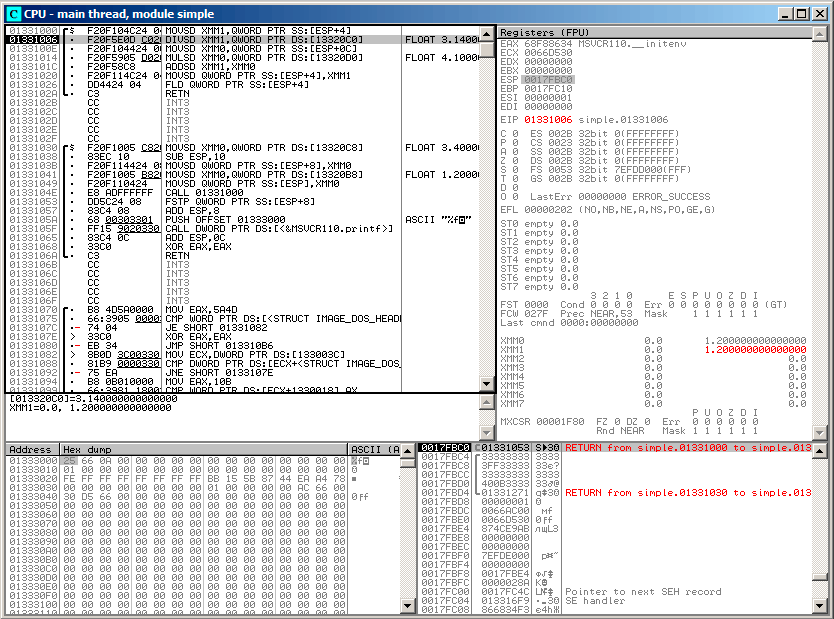
\includegraphics[scale=\FigScale]{patterns/205_floating_SIMD/simple_olly1.png}
\caption{\olly: \TT{MOVSD} \RU{загрузила значение}\EN{loads the value of} $a$ \RU{в}\EN{into} \XMM{1}}
\label{fig:FPU_SIMD_simple_olly1}
\end{figure}

\clearpage
\begin{figure}[H]
\centering
\includegraphics[scale=\FigScale]{patterns/205_floating_SIMD/simple_olly2.png}
\caption{\olly: \TT{DIVSD} \RU{вычислила}\EN{calculated} \gls{quotient} 
\RU{и оставила его в}\EN{and stored it in} \XMM{1}}
\label{fig:FPU_SIMD_simple_olly2}
\end{figure}

\clearpage
\begin{figure}[H]
\centering
\includegraphics[scale=\FigScale]{patterns/205_floating_SIMD/simple_olly3.png}
\caption{\olly: \TT{MULSD} \RU{вычислила}\EN{calculated} \gls{product} \RU{и оставила его в}\EN{and stored it
in} \XMM{0}}
\label{fig:FPU_SIMD_simple_olly3}
\end{figure}

\clearpage
\begin{figure}[H]
\centering
\includegraphics[scale=\FigScale]{patterns/205_floating_SIMD/simple_olly4.png}
\caption{\olly: \TT{ADDSD} \RU{прибавила значение в}\EN{adds value in} \XMM{0} \RU{к}\EN{to} \XMM{1}}
\label{fig:FPU_SIMD_simple_olly4}
\end{figure}

\clearpage
\begin{figure}[H]
\centering
\includegraphics[scale=\FigScale]{patterns/205_floating_SIMD/simple_olly5.png}
\caption{\olly: \FLD \RU{оставляет результат функции в}\EN{left function result in} \ST{0}}
\label{fig:FPU_SIMD_simple_olly5}
\end{figure}

\RU{Видно, что \olly показывает XMM-регистры как пары чисел в формате \Tdouble,
но используется только \IT{младшая} часть.}
\EN{We see that \olly shows the XMM registers as pairs of \Tdouble numbers,
but only the \IT{lower} part is used.}
\RU{Должно быть, \olly показывает их именно так, потому что сейчас исполняются SSE2-инструкции
с суффиксом \TT{-SD}.}
\EN{Apparently, \olly shows them in that format because the SSE2 instructions (suffixed with \TT{-SD}) 
are executed right now.}
\RU{Но конечно же, можно переключить отображение значений в регистрах и посмотреть содержимое
как 4 \Tfloat{}-числа или просто как 16 байт.}
\EN{But of course, it's possible to switch the register format and to see their contents as
4 \Tfloat{}-numbers or just as 16 bytes.}
\fi

\clearpage
\section{\RU{Передача чисел с плавающей запятой в аргументах}\EN{Passing floating point number via arguments}}

\lstinputlisting{patterns/12_FPU/2_passing_floats/pow.c}

\RU{Они передаются в младших половинах регистров}\EN{They are passed in the lower halves
of the} \XMM{0}-\XMM{3}\EN{ registers}.

\lstinputlisting[caption=\Optimizing MSVC 2012 x64]{patterns/205_floating_SIMD/pow_MSVC_2012_x64_Ox.asm}

\index{x86!\Instructions!MOVSD}
\index{x86!\Instructions!MOVSDX}
\RU{Инструкции}\EN{There is no} \TT{MOVSDX} \RU{нет в документации от}\EN{instruction in} 
Intel \cite{Intel} \AndENRU AMD \cite{AMD}\EN{ manuals}, 
\RU{там она называется просто}\EN{there it is called just} \TT{MOVSD}.
\RU{Таким образом, в процессорах x86 две инструкции с одинаковым именем}\EN{So there are two instructions
sharing the same name in x86} (\RU{о второй}\EN{about the other see}: \myref{REP_MOVSx}).
\RU{Возможно, в Microsoft решили избежать
путаницы и переименовали инструкцию в}\EN{Apparently, Microsoft developers wanted to get rid of the mess,
so they renamed it to} \TT{MOVSDX}.
\RU{Она просто загружает значение в младшую половину XMM-регистра}\EN{It just loads a value into
the lower half of a XMM register}.

\RU{Функция }\TT{pow()} \RU{берет аргументы из}\EN{takes arguments from} \XMM{0} \AndENRU \XMM{1}, 
\RU{и возвращает результат в}\EN{and returns result in} \XMM{0}.
\RU{Далее он перекладывается в}\EN{It is then moved to} \RDX \ForENRU \printf. 
\RU{Почему}\EN{Why}? 
\RU{Может быть, это потому что}\EN{Maybe because} 
\printf\EMDASH{}\RU{функция с переменным количеством аргументов}\EN{is a variable arguments function}?

\lstinputlisting[caption=\Optimizing GCC 4.4.6 x64]{patterns/205_floating_SIMD/pow_GCC446_x64_O3.s.\LANG}

GCC \RU{работает понятнее}\EN{generates clearer output}. 
\RU{Значение для}\EN{The value for} \printf \RU{передается в}\EN{is passed in} \XMM{0}. 
\RU{Кстати, вот тот случай, когда в}\EN{By the way, here is a case when 1 is written into} \EAX
\ForENRU \printf \RU{записывается 1 --- это значит, что будет передан один аргумент в векторных регистрах, 
так того требует стандарт}\EN{---this implies that one argument will be passed in vector registers,
just as the standard requires} \cite{SysVABI}.

\section{\RU{Пример с сравнением}\EN{Comparison example}}

\lstinputlisting{patterns/12_FPU/3_comparison/d_max.c}

\subsection{x64}

\lstinputlisting[caption=\Optimizing MSVC 2012 x64]{patterns/205_floating_SIMD/d_max_MSVC_2012_x64_Ox.asm}

\Optimizing MSVC \RU{генерирует очень понятный код}\EN{generates a code very easy to understand}.

\index{x86!\Instructions!COMISD}
\RU{Инструкция }\TT{COMISD} \RU{это}\EN{is} \q{Compare Scalar Ordered Double-Precision Floating-Point 
Values and Set EFLAGS}. \RU{Собственно, это она и делает}\EN{Essentially, that is what it does}.\\
\\
\NonOptimizing MSVC \RU{генерирует более избыточно, но тоже всё понятно}\EN{generates more redundant code,
but it is still not hard to understand}:

\lstinputlisting[caption=MSVC 2012 x64]{patterns/205_floating_SIMD/d_max_MSVC_2012_x64.asm}

\index{x86!\Instructions!MAXSD}
\RU{А вот}\EN{However,} GCC 4.4.6 \RU{дошел в оптимизации дальше и применил инструкцию}
\EN{did more optimizations and used the} \TT{MAXSD} (\q{Return Maximum Scalar 
Double-Precision Floating-Point Value})\RU{, которая просто выбирает максимальное значение}\EN{ instruction,
which just choose the maximum value}!

\lstinputlisting[caption=\Optimizing GCC 4.4.6 x64]{patterns/205_floating_SIMD/d_max_GCC446_x64_O3.s}

\clearpage
\subsection{x86}

\RU{Скомпилируем этот пример в MSVC 2012 с включенной оптимизацией:}
\EN{Let's compile this example in MSVC 2012 with optimization turned on:}

\lstinputlisting[caption=\Optimizing MSVC 2012 x86]{patterns/205_floating_SIMD/d_max_MSVC_2012_x86_Ox.asm}

\RU{Всё то же самое, только значения}\EN{Almost the same, but the values of} $a$ \AndENRU $b$ 
\RU{берутся из стека, а результат функции оставляется в}\EN{are taken from the stack and the function result 
is left in} \ST{0}.

\ifdefined\IncludeOlly
\RU{Если загрузить этот пример в}\EN{If we load this example in} \olly, 
\RU{увидим, как инструкция}\EN{we can see how the} \TT{COMISD} \RU{сравнивает значения и устанавливает/сбрасывает
флаги}\EN{instruction compares values and sets/clears the} \CF \AndENRU \PF\EN{ flags}:

\begin{figure}[H]
\centering
\includegraphics[scale=\FigScale]{patterns/205_floating_SIMD/d_max_olly.png}
\caption{\olly: \TT{COMISD} \RU{изменила флаги}\EN{changed} \CF \AndENRU \PF\EN{ flags}}
\label{fig:FPU_SIMD_d_max_olly}
\end{figure}
\fi

\section{\RU{Вычисление машинного эпсилона}\EN{Calculating machine epsilon}: x64 \AndENRU SIMD}
\label{machine_epsilon_x64_and_SIMD}

\RU{Вернемся к примеру \q{вычисление машинного эпсилона} для \Tdouble \lstref{machine_epsilon_double_c}.}
\EN{Let's revisit the \q{calculating machine epsilon} example for \Tdouble \lstref{machine_epsilon_double_c}.}

\RU{Теперь скомпилируем его для x64}\EN{Now we compile it for x64}:

\lstinputlisting[caption=\Optimizing MSVC 2012 x64]{patterns/205_floating_SIMD/epsilon_double_MSVC_2012_x64_Ox.asm}

\RU{Нет способа прибавить 1 к значению в 128-битном XMM-регистре, так что его нужно в начале поместить в память.}
\EN{There is no way to add 1 to a value in 128-bit XMM register, so it must be placed into memory.}

\RU{Впрочем, есть инструкция ADDSD (\IT{Add Scalar Double-Precision Floating-Point Values}),
которая может прибавить значение к младшей 64-битной части XMM-регистра игнорируя старшую половину,
но наверное MSVC 2012 пока недостаточно хорош для этого}
\EN{There is, however, the ADDSD instruction (\IT{Add Scalar Double-Precision Floating-Point Values}) 
which can add a value to the lowest 64-bit half of a XMM register while ignoring the higher one, 
but MSVC 2012 probably is not that good yet}
\footnote{\RU{В качестве упражнения, вы можете попробовать переработать этот код, чтобы избавиться 
от использования локального стека}\EN{As an exercise, you may try to rework this code to 
eliminate the usage of the local stack}.}.

\RU{Так или иначе, значение затем перезагружается в XMM-регистр и происходит вычитание.}
\EN{Nevertheless, the value is then reloaded to a XMM register and subtraction occurs.}
SUBSD \RU{это}\EN{is} \q{Subtract Scalar Double-Precision Floating-Point Values}, 
\RU{т.е. операция производится над младшей 64-битной частью 128-битного XMM-регистра}
\EN{i.e., it operates on the lower 64-bit part of 128-bit XMM register}.
\RU{Результат возвращается в регистре XMM0}\EN{The result is returned in the XMM0 register}.

\section{\RU{И снова пример генератора случайных чисел}\EN{Pseudo-random number generator example revisited}}
\label{FPU_PRNG_SIMD}

\RU{Вернемся к примеру \q{пример генератора случайных чисел} \lstref{FPU_PRNG}.}
\EN{Let's revisit \q{pseudo-random number generator example} example \lstref{FPU_PRNG}.}

\RU{Если скомпилировать это в MSVC 2012, компилятор будет использовать SIMD-инструкции для FPU.}
\EN{If we compile this in MSVC 2012, it will use the SIMD instructions for the FPU.}

\lstinputlisting[caption=\Optimizing MSVC 2012]{patterns/205_floating_SIMD/FPU_PRNG/MSVC2012_Ox_Ob0.asm.\LANG}

% FIXME1 rewrite!
\RU{У всех инструкций суффикс -SS, это означает \q{Scalar Single}.}
\EN{All instructions have the -SS suffix, which stands for \q{Scalar Single}.}
\RU{\q{Scalar} означает что только одно значение хранится в регистре.}
\EN{\q{Scalar} implies that only one value is stored in the register.}
\RU{\q{Single} означает что это тип \Tfloat.}
\EN{\q{Single} stands for \Tfloat data type.}


\section{\RU{Итог}\EN{Summary}}

\RU{Во всех приведенных примерах, в XMM-регистрах используется только младшая половина регистра, там
хранится значение в формате IEEE 754}\EN{Only the lower half of XMM registers is used in all examples here, 
to store number in IEEE 754 format}.

\RU{Собственно, все инструкции с суффиксом}\EN{Essentially, all instructions prefixed by} 
\TT{-SD} (\q{Scalar Double-Precision})\EMDASH{}\RU{это инструкции для работы с числами с плавающей 
запятой в формате IEEE 754, 
хранящиеся в младшей 64-битной половине XMM-регистра}\EN{are instructions working with floating point numbers
in IEEE 754 format, stored in the lower 64-bit half of a XMM register}.

\RU{Всё удобнее чем это было в FPU, видимо, сказывается тот факт, что расширения 
SIMD развивались не так хаотично как FPU в прошлом.}
\EN{And it is easier than in the FPU, probably because the SIMD extensions 
were evolved in a less chaotic way than the FPU ones in the past.}
\RU{Стековая модель регистров не используется}\EN{The stack register model is not used}.

\index{x86!\Instructions!ADDSS}
\index{x86!\Instructions!MOVSS}
\index{x86!\Instructions!COMISS}
% TODO1: do this!
\RU{Если вы попробуете заменить в этих примерах}\EN{If you would try to replace} \Tdouble \RU{на}\EN{with} \Tfloat
\RU{, то инструкции будут использоваться те же,
только с суффиксом}
% FIXME1 ... but their -SS versions
\EN{in these examples, the same instructions will be used, but prefixed with} \TT{-SS} 
(\q{Scalar Single-Precision}), \RU{например}\EN{for example}, \TT{MOVSS}, \TT{COMISS}, \TT{ADDSS}, \etc{}.

\q{Scalar} \RU{означает что SIMD-регистр будет хранить только одно значение, вместо нескольких.}
\EN{implies that the SIMD register containing only one value instead of several.}
\RU{Инструкции, работающие с несколькими значениями в регистре одновременно, имеют \q{Packed} в названии}
\EN{Instructions working with several values in a register simultaneously have \q{Packed} in their name}.

\RU{Нужно также обратить внимание, что SSE2-инструкции работают с 64-битными числами (\Tdouble) в формате IEEE 754,
в то время как внутреннее представление в FPU --- 80-битные числа.}
\EN{Needless to say, the SSE2 instructions work with 64-bit IEEE 754 numbers (\Tdouble),
while the internal representation of the floating-point numbers in FPU is 80-bit numbers.}
\RU{Поэтому ошибок округления (\IT{round-off error}) в FPU может быть меньше чем в SSE2,
как следствие, можно сказать, работа с FPU может давать более точные результаты вычислений.}
\EN{Hence, the FPU may produce less round-off errors and as a consequence, FPU may give more precise
calculation results.}

\fi
\ifdefined\IncludeARM
\chapter{\EN{ARM-specific details}\RU{Кое-что специфичное для ARM}}

\section{\RU{Знак номера}\EN{Number sign} (\#) \RU{перед числом}\EN{before number}}

\RU{Компилятор Keil, \IDA и objdump предваряет все числа знаком номера (\q{\#}), например:}
\EN{The Keil compiler, \IDA and objdump precede all numbers with the \q{\#} number sign, for example:}
\lstref{Keil_number_sign}.
\RU{Но когда GCC 4.9 выдает результат на языке ассемблера, он так не делает, например:}
\EN{But when GCC 4.9 generates assembly language output, it doesn't, for example: }
\lstref{GCC_no_number_sign}.

\RU{Так что листинги для ARM в этой книге в каком-то смысле перемешаны.}
\EN{The ARM listings in this book are somewhat mixed.}

\RU{Трудно сказать, как правильнее.}\EN{It's hard to say, which method is right.}
\RU{Должно быть, всякий должен придерживаться тех правил, которые приняты в той среде, в которой он работает.}%
\EN{Supposedly, one has to obey the rules accepted in environment he/she works in.}

% sections
\section{\RU{Режимы адресации}\EN{Addressing modes}}
\index{ARM!\RU{Режимы адресации}\EN{Addressing modes}}
\label{ARM_postindex_vs_preindex}
\index{\CLanguageElements!\PostIncrement}
\index{\CLanguageElements!\PostDecrement}
\index{\CLanguageElements!\PreIncrement}
\index{\CLanguageElements!\PreDecrement}

\EN{This instruction is possible in ARM64:}
\RU{В ARM64 возможна такая инструкция:}

\index{ARM!\Instructions!LDR}
\begin{lstlisting}
ldr	x0, [x29,24]
\end{lstlisting}

\EN{This means add 24 to the value in X29 and load the value from this address.}
\RU{И это означает прибавить 24 к значению в X29 и загрузить значение по этому адресу.}
\RU{Обратите внимание что 24 внутри скобок.}
\EN{Please note that 24 is inside the brackets.}
\EN{The meaning is different if the number is outside the brackets:}
\RU{А если снаружи скобок, то весь смысл меняется:}

\begin{lstlisting}
ldr	w4, [x1],28
\end{lstlisting}

\RU{Это означает, загрузить значение по адресу в X1, затем прибавить 28 к X1.}
\EN{This means load the value at the address in X1, then add 28 to X1.}

\index{PDP-11}
\RU{ARM позволяет прибавлять некоторую константу к адресу, с которого происходит загрузка, либо вычитать.}
\EN{ARM allows you to add or subtract a constant to/from the address used for loading.}
\RU{Причем, позволяет это делать до загрузки или после.}
\EN{And it's possible to do that both before and after loading.}

\RU{Такого режима адресации в x86 нет, но он есть в некоторых других процессорах, даже на PDP-11.}
\EN{There is no such addressing mode in x86, but it is present in some other processors, even on PDP-11.}
\RU{Существует байка, что режимы пре-инкремента, пост-инкремента, 
пре-декремента и пост-декремента адреса в PDP-11}
\EN{There is a legend that the pre-increment, post-increment, pre-decrement and post-decrement modes in PDP-11},
\RU{были \q{виновны} в появлении таких конструкций языка Си (который разрабатывался на PDP-11) как}
\EN{were \q{guilty} for the appearance of such C language (which developed on PDP-11) constructs as}
*ptr++, *++ptr, *ptr-{}-, *-{}-ptr. 
\RU{Кстати, это является трудно запоминаемой особенностью в Си.}
\EN{By the way, this is one of the hard to memorize C features.}
\RU{Дела обстоят так:}\EN{This is how it is:}

% FIXME: add ARM assembly...
\begin{center}
\begin{tabular}{ | l | l | l | l | }
\hline
\headercolor{} \RU{термин в Си}\EN{C term} & 
\headercolor{} \RU{термин в ARM}\EN{ARM term} & 
\headercolor{} \RU{выражение Си}\EN{C statement} & 
\headercolor{} \RU{как это работает}\EN{how it works} \\
\hline
\PostIncrement & 
post-indexed addressing & 
\TT{*ptr++} & 
\RU{использовать значение \TT{*ptr}}\EN{use \TT{*ptr} value}, \\
& & & \RU{затем инкремент указателя \TT{ptr}}\EN{then \gls{increment} \TT{ptr} pointer} \\
\hline
\PostDecrement & 
post-indexed addressing & 
\TT{*ptr-{}-} & 
\RU{использовать значение \TT{*ptr}}\EN{use \TT{*ptr} value}, \\
& & & \RU{затем \glslink{decrement}{декремент} указателя \TT{ptr}}\EN{then \gls{decrement} \TT{ptr} pointer} \\
\hline
\PreIncrement & 
pre-indexed addressing & 
\TT{*++ptr} & 
\RU{инкремент указателя \TT{ptr}}\EN{\gls{increment} \TT{ptr} pointer}, \\
& & & \RU{затем использовать значение \TT{*ptr}}\EN{then use \TT{*ptr} value} \\
\hline
\PreDecrement & 
pre-indexed addressing & 
\TT{*-{}-ptr} & 
\RU{\glslink{decrement}{декремент} указателя \TT{ptr}}\EN{\gls{decrement} \TT{ptr} pointer}, \\
& & & \RU{затем использовать значение \TT{*ptr}}\EN{then use \TT{*ptr} value} \\
\hline
\end{tabular}
\end{center}

Pre-indexing \EN{is marked with an exclamation mark in the ARM assembly language}\RU{маркируется как 
восклицательный знак в ассемблере ARM}.
\RU{Для примера, смотрите строку 2 в}\EN{For example, see line 2 in} \lstref{hw_ARM64_GCC}.

\RU{Деннис Ритчи (один из создателей ЯП Си) указывал, что, это, вероятно, придумал Кен Томпсон 
(еще один создатель Си),
потому что подобная возможность процессора имелась еще в PDP-7}
\EN{Dennis Ritchie (one of the creators of the C language) mentioned that it probably was invented by Ken Thompson
(another C creator) because this processor feature was present in PDP-7}
\cite{Ritchie:1986}\cite{Ritchie:1993:DCL:155360.155580}.
\RU{Таким образом, компиляторы с ЯП Си на тот процессор, где это есть, могут использовать это.}
\EN{Thus, C language compilers may use it, if it is present on the target processor.}

\RU{Всё это очень удобно для работы с массивами.}
\EN{That's very convenient for array processing.}

\section{\RU{Загрузка констант в регистр}\EN{Loading a constant into a register}}
\label{ARM_big_constants}

\subsection{\RU{32-битный}\EN{32-bit} ARM}
\label{ARM_big_constants_loading}

\RU{Как мы уже знаем, все инструкции имеют длину в 4 байта в режиме ARM и 2 байта в режиме Thumb.}
\EN{Aa we already know, all instructions have a length of 4 bytes in ARM mode and 2 bytes in Thumb mode.}
\RU{Как в таком случае записать в регистр 32-битное число, если его невозможно закодировать
внутри одной инструкции?}
\EN{Then how can we load a 32-bit value into a register, if it's not possible to encode it in one instruction?}

\RU{Попробуем}\EN{Let's try}:

\begin{lstlisting}
unsigned int f()
{
	return 0x12345678;
};
\end{lstlisting}

\begin{lstlisting}[caption=GCC 4.6.3 -O3 \ARMMode]
f:
        ldr     r0, .L2
        bx      lr
.L2:
        .word   305419896 ; 0x12345678
\end{lstlisting}

\RU{Т.е., значение \TT{0x12345678} просто записано в памяти отдельно и загружается, если нужно.}
\EN{So, the \TT{0x12345678} value is just stored aside in memory and loaded if needed.}
\RU{Но можно обойтись и без дополнительного обращения к памяти.}
\EN{But it's possible to get rid of the additional memory access.}

\begin{lstlisting}[caption=GCC 4.6.3 -O3 -march{=}armv7-a (\ARMMode)]
movw    r0, #22136      ; 0x5678
movt    r0, #4660       ; 0x1234
bx      lr
\end{lstlisting}

\RU{Видно, что число загружается в регистр по частям, в начале младшая часть 
(при помощи инструкции MOVW), затем старшая (при помощи MOVT).}
\EN{We see that the value is loaded into the register by parts, the lower part first (using MOVW), 
then the higher (using MOVT).}

\RU{Следовательно, нужно 2 инструкции в режиме ARM, чтобы записать 32-битное число в регистр.}
\EN{This implies that 2 instructions are necessary in ARM mode for loading a 32-bit value into a register.}
\RU{Это не так уж и страшно, потому что в реальном коде не так уж и много констант (кроме 0 и 1).}
\EN{It's not a real problem, because in fact there are not many constants in real code (except of 0 and 1).}
\RU{Значит ли это, что это исполняется медленнее чем одна инструкция, как две инструкции?}
\EN{Does it mean that the two-instruction version is slower than one-instruction version?}
\RU{Вряд ли, наверняка современные процессоры ARM наверняка умеют распознавать такие 
последовательности и исполнять их быстро.}
\EN{Doubtfully. Most likely, modern ARM processors are able to detect such sequences and execute
them fast.}

\RU{А \IDA легко распознает подобные паттерны в коде и дизассемблирует эту функцию как:}
\EN{On the other hand, \IDA is able to detect such patterns in the code and disassembles this function as:}

\begin{lstlisting}
MOV    R0, 0x12345678
BX     LR
\end{lstlisting}

\subsection{ARM64}

\begin{lstlisting}
uint64_t f()
{
	return 0x12345678ABCDEF01;
};
\end{lstlisting}

\begin{lstlisting}[caption=GCC 4.9.1 -O3]
mov	x0, 61185   ; 0xef01
movk	x0, 0xabcd, lsl 16
movk	x0, 0x5678, lsl 32
movk	x0, 0x1234, lsl 48
ret
\end{lstlisting}

\index{ARM!\Instructions!MOVK}
\TT{MOVK} \RU{означает}\EN{stands for} \q{MOV Keep}, \RU{т.е. она записывает 16-битное значение в регистр, не трогая
при этом остальные биты.}\EN{i.e., it writes a 16-bit value into the register, not touching the rest of the bits.}
\index{ARM!Optional operators!LSL}
\EN{The}\RU{Суффикс} \TT{LSL} \RU{сдвигает значение в каждом случае влево на 16, 32 и 48 бит. Сдвиг происходит
перед загрузкой.}\EN{suffix shifts left the value by 16, 32 and 48 bits at each step. The shifting is done before loading.}
\RU{Таким образом, нужно 4 инструкции, чтобы записать в регистр 64-битное значение.}
\EN{This implies that 4 instructions are necessary to load a 64-bit value into a register.}

\subsubsection{\RU{Записать числа с плавающей точкой в регистр}\EN{Storing floating-point number into register}}

\RU{Некоторые числа можно записывать в D-регистр при помощи только одной инструкции.}
\EN{It's possible to store a floating-point number into a D-register using only one instruction.}

\RU{Например}\EN{For example}:

\begin{lstlisting}
double a()
{
	return 1.5;
};
\end{lstlisting}

\begin{lstlisting}[caption=GCC 4.9.1 -O3 + objdump]
0000000000000000 <a>:
   0:   1e6f1000        fmov    d0, #1.500000000000000000e+000
   4:   d65f03c0        ret
\end{lstlisting}

\RU{Число $1.5$ действительно было закодировано в 32-битной инструкции.}
\EN{The number $1.5$ was indeed encoded in a 32-bit instruction.}
\RU{Но как}\EN{But how}?
\index{ARM!\Instructions!FMOV}
\RU{В ARM64, инструкцию \TT{FMOV} есть 8 бит для кодирования некоторых чисел с плавающей запятой.}
\EN{In ARM64, there are 8 bits in the \TT{FMOV} instruction for encoding some floating-point numbers.}
\RU{В \cite{ARM64ref} алгоритм называется \TT{VFPExpandImm()}.}
\EN{The algorithm is called \TT{VFPExpandImm()} in \cite{ARM64ref}.}
\index{minifloat}
\EN{This is also called}\RU{Это также называется} \IT{minifloat}\footnote{\href{http://go.yurichev.com/17139}{wikipedia}}.
\RU{Мы можем попробовать разные: $30.0$ и $31.0$ компилятору удается закодировать, а $32.0$ уже нет, для него
приходится выделять 8 байт в памяти и записать его там в формате IEEE 754:}
\EN{We can try different values: the compiler is able to encode $30.0$ and $31.0$, but it couldn't encode $32.0$,
as 8 bytes have to be allocated for this number in the IEEE 754 format:}

\begin{lstlisting}
double a()
{
	return 32;
};
\end{lstlisting}

\begin{lstlisting}[caption=GCC 4.9.1 -O3]
a:
	ldr	d0, .LC0
	ret
.LC0:
	.word	0
	.word	1077936128
\end{lstlisting}

\section{\RU{Релоки}\EN{Relocs} \InENRU ARM64}
\label{ARM64_relocs}

\RU{Как известно, в ARM64 инструкции 4-байтные, так что записать длинное число в регистр одной инструкцией нельзя.}
\EN{As we know, there are 4-byte instructions in ARM64, so it is impossible to write a large number into a register
using a single instruction.}
\RU{Тем не менее, файл может быть загружен по произвольному адресу в памяти, для этого релоки и нужны.}
\EN{Nevertheless, an executable image can be loaded at any random address in memory, so that's why relocs exists.}
\RU{Больше о них (в связи с Win32 PE)}\EN{Read more about them (in relation to Win32 PE)}: \myref{subsec:relocs}.

\index{ARM!\Instructions!ADRP/ADD pair}
\RU{В ARM64 принят следующий метод: адрес формируется при помощи пары инструкций: \TT{ADRP} и \ADD.}
\EN{The address is formed using the \TT{ADRP} and \ADD instruction pair in ARM64.}
\RU{Первая загружает в регистр адрес 4KiB-страницы, а вторая прибавляет остаток.}
\EN{The first loads a 4KiB-page address and the second one adds the remainder.}
\RU{Скомпилируем пример из}\EN{Let's compile the example from} \q{\HelloWorldSectionName} 
(\lstref{hw_c}) \InENRU GCC (Linaro) 4.9 \RU{под}\EN{under} win32:

\begin{lstlisting}[caption=GCC (Linaro) 4.9 \AndENRU objdump \EN{of object file}\RU{объектного файла}]
...>aarch64-linux-gnu-gcc.exe hw.c -c

...>aarch64-linux-gnu-objdump.exe -d hw.o

...

0000000000000000 <main>:
   0:   a9bf7bfd        stp     x29, x30, [sp,#-16]!
   4:   910003fd        mov     x29, sp
   8:   90000000        adrp    x0, 0 <main>
   c:   91000000        add     x0, x0, #0x0
  10:   94000000        bl      0 <printf>
  14:   52800000        mov     w0, #0x0                        // #0
  18:   a8c17bfd        ldp     x29, x30, [sp],#16
  1c:   d65f03c0        ret

...>aarch64-linux-gnu-objdump.exe -r hw.o

...

RELOCATION RECORDS FOR [.text]:
OFFSET           TYPE              VALUE
0000000000000008 R_AARCH64_ADR_PREL_PG_HI21  .rodata
000000000000000c R_AARCH64_ADD_ABS_LO12_NC  .rodata
0000000000000010 R_AARCH64_CALL26  printf
\end{lstlisting}

\RU{Итак, в этом объектом файле три релока.}
\EN{So there are 3 relocs in this object file.}

\begin{itemize}
\item 
\RU{Самый первый берет адрес страницы, отсекает младшие 12 бит и записывает оставшиеся старшие 21
в битовые поля инструкции \TT{ADRP}. Это потому что младшие 12 бит кодировать не нужно,
и в ADRP выделено место только для 21 бит.}
\EN{The first one takes the page address, cuts the lowest 12 bits and writes the remaining high 21 bits
to the \TT{ADRP} instruction's bit fields. This is because we don't need to encode the low 12 bits,
and the ADRP instruction has space only for 21 bits.}

\item \RU{Второй ---- 12 бит адреса, относительного от начала страницы, в поля инструкции \ADD.}
\EN{The second one puts the 12 bits of the address relative to the page start into the \ADD instruction's bit fields.}

\item \RU{Последний, 26-битный, накладывается на инструкцию по адресу \TT{0x10}, где переход на функцию \printf.}
\EN{The last, 26-bit one, is applied to the instruction at address \TT{0x10} where the 
jump to the \printf function is.}
\RU{Все адреса инструкций в ARM64 (да и в ARM в режиме ARM) имеют нули в двух младших битах
(потому что все инструкции имеют размер в 4 байта),
так что нужно кодировать только старшие 26 бит из 28-битного адресного пространства ($\pm 128$MB).}
\EN{All ARM64 (and in ARM in ARM mode) instruction addresses have zeroes in the two lowest bits
(because all instructions have a size of 4 bytes),
so one need to encode only the highest 26 bits of 28-bit address space ($\pm 128$MB).}

\end{itemize}

\RU{В слинкованном исполняемом файле релоков в этих местах нет: потому что там уже точно известно, 
где будет находится строка \q{Hello!}, и в какой странице, а также известен адрес функции \puts.}
\EN{There are no such relocs in the executable file: because it's known where the \q{Hello!} string
is located, in which page, and the address of \puts is also known.}
\RU{И поэтому там, в инструкциях \TT{ADRP}, \ADD и \TT{BL}, уже проставлены нужные значения 
(их проставил линкер во время компоновки):}
\EN{So there are values set already in the \TT{ADRP}, \ADD and \TT{BL} instructions
(the linker has written them while linking):}

\begin{lstlisting}[caption=objdump \EN{of executable file}\RU{исполняемого файла}]
0000000000400590 <main>:
  400590:       a9bf7bfd        stp     x29, x30, [sp,#-16]!
  400594:       910003fd        mov     x29, sp
  400598:       90000000        adrp    x0, 400000 <_init-0x3b8>
  40059c:       91192000        add     x0, x0, #0x648
  4005a0:       97ffffa0        bl      400420 <puts@plt>
  4005a4:       52800000        mov     w0, #0x0                        // #0
  4005a8:       a8c17bfd        ldp     x29, x30, [sp],#16
  4005ac:       d65f03c0        ret

...

Contents of section .rodata:
 400640 01000200 00000000 48656c6c 6f210000  ........Hello!..
\end{lstlisting}

\index{ARM!\Instructions!BL}

\ifdefined\ENGLISH{}
As an example, let's try to disassemble the BL instruction manually.\\
\TT{0x97ffffa0} is $10010111111111111111111110100000b$.
According to \cite[C5.6.26]{ARM64ref}, \IT{imm26} is the last 26 bits: $imm26 = 11111111111111111110100000$.
It is \TT{0x3FFFFA0}, but the \ac{MSB} is 1, 
so the number is negative, and we can convert it manually to convenient form for us.
By the rules of negation (\myref{sec:signednumbers:negation}), just invert all bits: (it is \TT{1011111=0x5F}), and add 1 (\TT{0x5F+1=0x60}).
So the number in signed form is \TT{-0x60}.
Let's multiplicate \TT{-0x60} by 4 (because address stored in opcode is divided by 4): it is \TT{-0x180}.
Now let's calculate destination address: \TT{0x4005a0} + (\TT{-0x180}) = \TT{0x400420} 
(please note: we consider the address of the BL instruction, not the current value of \ac{PC}, which may be different!).
So the destination address is \TT{0x400420}.\\
\\
More about ARM64-related relocs: \cite{ARM64_ELF}.
\fi

\ifdefined\RUSSIAN{}
В качестве примера, попробуем дизассемблировать инструкцию BL вручную.\\
\TT{0x97ffffa0} это $10010111111111111111111110100000b$.
В соответствии с \cite[C5.6.26]{ARM64ref}, \IT{imm26} это последние 26 бит: $imm26 = 11111111111111111110100000$.
Это \TT{0x3FFFFA0}, но \ac{MSB} это 1, 
так что число отрицательное, мы можем вручную его конвертировать в удобный для нас вид.
По правилам изменения знака (\myref{sec:signednumbers:negation}), просто инвертируем все биты: (\TT{1011111=0x5F}) и прибавляем 1 (\TT{0x5F+1=0x60}).
Так что число в знаковом виде: \TT{-0x60}.
Умножим \TT{-0x60} на 4 (потому что адрес записанный в опкоде разделен на 4): это \TT{-0x180}.
Теперь вычисляем адрес назначения: \TT{0x4005a0} + (\TT{-0x180}) = \TT{0x400420} 
(пожалуйста заметьте: мы берем адрес инструкции BL, а не текущее значение \ac{PC}, которое может быть другим!).
Так что адрес в итоге \TT{0x400420}.\\
\\
Больше о релоках связанных с ARM64: \cite{ARM64_ELF}.
\fi


\fi
\ifdefined\IncludeMIPS
\chapter{\EN{MIPS-specific details}\RU{Кое-что специфичное для MIPS}}

% sections
\section{\RU{Загрузка констант в регистр}\EN{Loading constants into register}}
\label{MIPS_big_constants}

\begin{lstlisting}
unsigned int f()
{
	return 0x12345678;
};
\end{lstlisting}

\RU{В MIPS, так же как и в ARM, все инструкции имеют размер 32 бита, так что невозможно
закодировать 32-битную константу в инструкцию.}
\EN{All instructions in MIPS, just like ARM, have a of 32-bit, so it's not possible to
embed a 32-bit constant into one instruction.}
\index{MIPS!\Instructions!LI}
\index{MIPS!\Instructions!ORI}
\RU{Так что это транслируется в две инструкции:
первая загружает старшую часть 32-битного числа и вторая применяет операцию \q{ИЛИ},
эффект от которой в том, что она просто выставляет младшие 16 бит целевого регистра:}
\EN{So this translates to at least two instructions: 
the first loads the high part of the 32-bit number and the second
one applies an OR operation, which effectively sets the low 16-bit part of the target register:}

\begin{lstlisting}[caption=GCC 4.4.5 -O3 (\assemblyOutput)]
        li      $2,305397760                    # 0x12340000
        j       $31
        ori     $2,$2,0x5678 ; branch delay slot
\end{lstlisting}

\IDA \RU{знает о таких часто встречающихся последовательностях, так что для удобства, 
она показывает последнюю инструкцию ORI как псевдоинструкцию LI, 
которая якобы загружает полное 32-битное значение в регистр \$V0.}
\EN{is fully aware of such frequently encountered code patterns, 
so, for convenience it shows the last ORI instruction as the LI pseudoinstruction,
which allegedly loads a full 32-bit number into the \$V0 register.}

\index{MIPS!\Instructions!LUI}

\begin{lstlisting}[caption=GCC 4.4.5 -O3 (IDA)]
         lui     $v0, 0x1234
         jr      $ra
         li      $v0, 0x12345678 ; branch delay slot
\end{lstlisting}

\RU{В выводе на ассемблере от GCC есть псевдоинструкция LUI, но на самом деле, 
там LUI (\q{Load Upper Immediate}), загружающая 16-битное значение в старшую часть регистра.}
\EN{The GCC assembly output has the LI pseudoinstruction, but in fact, LUI (\q{Load Upper Imeddiate}) is there,
which stores a 16-bit value into the high part of the register.}


\section{\RU{Книги и прочие материалы о MIPS}\EN{Further reading about MIPS}}

\cite{MIPSRun}.

\fi
